% This is a combination of pandoc's default latex template:
%DIF LATEXDIFF DIFFERENCE FILE
%DIF DEL dissertation_v2.tex   Sun Dec 12 11:42:55 2021
%DIF ADD dissertation_v3.tex   Mon Dec 13 00:35:38 2021
% https://github.com/jgm/pandoc/blob/master/data/templates/default.latex

% and Dylan Mikesell's BSU thesis template:
% https://github.com/dylanmikesell/BSU_LaTeX_Thesis_Template/blob/master/src/BSUmain.tex

% and Dylan Mikesell's BSU style file:
% https://github.com/dylanmikesell/BSU_LaTeX_Thesis_Template/blob/master/src/BSUthesis.sty

% For BSU style requirements see:
% https://github.com/dylanmikesell/BSU_LaTeX_Thesis_Template/blob/master/src/BSU_checklist.pdf

% Pass options to packages loaded elsewhere
  \PassOptionsToPackage{dvipsnames,svgnames,x11names}{xcolor}

% Document class options
% Note: everything defined between \documentclass{} and \begin{document}
% is the "preamble"
\documentclass[
      12pt,
          twoside]{report}

% Loading packages and options

% Page geometry settings
\usepackage[
  left=1.5in,
  right=1in,
  top=1in,
  bottom=1in,
  letterpaper,
  includehead,
  includefoot,
  headheight=14.5pt
]{geometry}

% For colors
\usepackage[table]{xcolor} % Handles colors

% For better hyphenations
\usepackage{soulutf8}

% For landscape pages
\usepackage{pdflscape}

% For making corrections to functions
\usepackage{etoolbox}

% For strikeout and underline text
\usepackage[normalem]{ulem}

% Linespacing using setspace package
\usepackage{setspace}
\setstretch{2} % double space

% Math packages
\usepackage{amsmath,amssymb}

% Textcase for handling upper/lower case
\usepackage{textcase}

% Changepage package for changing layout in the middle of a document
\usepackage{changepage}

% For month year format
\usepackage{datetime}

% For chapter (and other) headings required by BSU
\usepackage{fancyhdr}

% Set captions styling
\usepackage[labelfont=bf,textfont=bf]{caption}
\captionsetup[figure]{
  font={
    stretch=0.6,
          small
      }
}

% For better float environments
\usepackage{float}

% For making tables and final reading approval page
\usepackage{tabularx}

% For setting (sub)section heading formatting and first paragraph spacing
\usepackage[explicit]{titlesec}

% For TOC style
\usepackage{titletoc}

% Font encoding
% Defaults to 8-bit T1 encoding with 256 glyphs
% https://ctan.org/pkg/encguide
% http://www.micropress-inc.com/fonts/encoding/t1.htm
\usepackage[T1]{fontenc}
\usepackage[utf8]{inputenc}
% Font family setting
  \usepackage{kpfonts}

% Use upquote if available, for straight quotes in verbatim environments
\IfFileExists{upquote.sty}{\usepackage{upquote}}{}
\IfFileExists{microtype.sty}{% use microtype if available
  \usepackage[]{microtype}
  \UseMicrotypeSet[protrusion]{basicmath} % disable protrusion for tt fonts
}{}

% Allow pandoc to inject code highlighting environments

% Tables settings
\usepackage{booktabs,array,threeparttable}
\usepackage{multirow}
\usepackage{calc} % for calculating minipage widths

% Correct order of tables after \paragraph or \subparagraph
%\makeatletter
%\patchcmd\longtable{\par}{\if@noskipsec\mbox{}\fi\par}{}{}
%\makeatother

% Block quote shaded style
\usepackage{framed}
\AtBeginEnvironment{quote}{\par\singlespacing\small}
\let\oldquote=\quote
\let\endoldquote=\endquote
\colorlet{shadecolor}{gray!15}
\renewenvironment{quote}{\begin{shaded*}\begin{oldquote}}{\end{oldquote}\end{shaded*}}

% Allow footnotes in longtable head/foot
%\IfFileExists{footnotehyper.sty}{\usepackage{footnotehyper}}{\usepackage{footnote}}
%\makesavenoteenv{longtable}

% Graphics settings
\usepackage{graphicx}
\makeatletter
\def\maxwidth{\ifdim\Gin@nat@width>\linewidth\linewidth\else\Gin@nat@width\fi}
\def\maxheight{\ifdim\Gin@nat@height>\textheight\textheight\else\Gin@nat@height\fi}
\makeatother

% Scale images if necessary, so that they will not overflow the page
% margins by default, and it is still possible to overwrite the defaults
% using explicit options in \includegraphics[width, height, ...]{}
\setkeys{Gin}{width=\maxwidth,height=\maxheight,keepaspectratio}
% Set default figure placement to htbp
\makeatletter
\def\fps@figure{htbp}
\makeatother

% Prevent overfull lines
\setlength{\emergencystretch}{3em}
\providecommand{\tightlist}{\setlength{\itemsep}{0pt}\setlength{\parskip}{0pt}}

% Csl environment (required by pandoc)
  \newlength{\cslhangindent}
  \setlength{\cslhangindent}{1.5em}
  \newlength{\csllabelwidth}
  \setlength{\csllabelwidth}{3em}
  \newlength{\cslentryspacingunit} % times entry-spacing
  \setlength{\cslentryspacingunit}{\parskip}
  \newenvironment{CSLReferences}[2] % #1 hanging-ident, #2 entry spacing
   {% don't indent paragraphs
    \setlength{\parindent}{0pt}
    % turn on hanging indent if param 1 is 1
    \ifodd #1
    \let\oldpar\par
    \def\par{\hangindent=\cslhangindent\oldpar}
    \fi
    % set entry spacing
    \setlength{\parskip}{#2\cslentryspacingunit}
   }%
   {}
  \usepackage{calc}
  \newcommand{\CSLBlock}[1]{#1\hfill\break}
  \newcommand{\CSLLeftMargin}[1]{\parbox[t]{\csllabelwidth}{#1}}
  \newcommand{\CSLRightInline}[1]{\parbox[t]{\linewidth - \csllabelwidth}{#1}\break}
  \newcommand{\CSLIndent}[1]{\hspace{\cslhangindent}#1}

% Expand header includes
  \usepackage{booktabs}
  \usepackage{longtable}
  \usepackage{array}
  \usepackage{multirow}
  \usepackage{wrapfig}
  \usepackage{float}
  \usepackage{colortbl}
  \usepackage{pdflscape}
  \usepackage{tabu}
  \usepackage{threeparttable}
  \usepackage{threeparttablex}
  \usepackage[normalem]{ulem}
  \usepackage{makecell}
  \usepackage{xcolor}

% Bibliography settings
% Natbib settings

% Nocite

% Some options for hyperlinks
\usepackage[bookmarks=true,pageanchor=false]{hyperref}
\hypersetup{
      colorlinks=true,
    linkcolor={Brown},
    filecolor={Brown},
    citecolor={CornflowerBlue},
    urlcolor={Blue}
  }
\usepackage{xurl} % add URL line breaks if available
\usepackage{bookmark}
\urlstyle{same} % disable monospaced font for URLs

% Abbreviations and acronyms
\usepackage[nonumberlist,acronym,toc]{glossaries-extra}
% http://ctan.mirrors.hoobly.com/macros/latex/contrib/glossaries/glossariesbegin.pdf
\setabbreviationstyle[acronym]{long-short} % glossaries-extra.sty only
% For abbreviations
  \makeglossaries
  \loadglsentries{assets/tex/abbreviations}

% Nomenclature
\usepackage[noprefix,intoc]{nomencl}
% For symbols and nomenclature 
  \makenomenclature
  \nomenclature{$^{\circ}C$}{Celcius}
\nomenclature{$Ma$}{\textit{Mega annum} or million-years}
\nomenclature{$GPa$}{Gigapascal}
\nomenclature{$K$}{Kelvin}
\nomenclature{$wt.\%$}{weight percent}
\nomenclature{$km$}{kilometer}
\nomenclature{$\vec{q}$}{surface heat flow}
\nomenclature{$\Phi$}{Thermal parameter}
\nomenclature{$\vec{v}_{conv}$}{convergence velocity}
\nomenclature{$t_{OP}$}{oceanic plate age}
\nomenclature{$Z_{UP}$}{Upper plate thickness}
\nomenclature{$Z_{cpl}$}{Mechanical coupling depth}
\nomenclature{$\eta$}{viscosity}


%% End packages and options

% Frontmatter pages (title, approval, copyright)

% Make title page
  \title{Computational Approaches to Understanding Subduction Geodynamics, Surface Heat Flow, and the Metamorphic Rock Record}

% Change title of contents name
\renewcommand{\contentsname}{Table of contents}

\def\maketitle{
  \cleardoublepage
  \begin{titlepage}
    \pagenumbering{roman}
    \begin{center}
        % Title
        {\huge Computational Approaches to Understanding Subduction Geodynamics, Surface Heat Flow, and the Metamorphic Rock Record \par}
        \vspace*{0.5in}

        % Author
        {by\\}
        {Buchanan C. Kerswell}
        \vspace*{1in}

        % Description
        A dissertation\\
        submitted in partial fulfillment \\
        of the requirements for the degree of\\
        Doctor of Philosophy~in~Geosciences\\
        Boise State University
        \vspace*{0.5in}

        % Date
        November 2021
    \end{center}
  \end{titlepage}
  \let\maketitle\relax
}

% Make final reading approval page
\def\makesubmittalsheet{
  \cleardoublepage 
  \begin{center}
    BOISE STATE UNIVERSITY GRADUATE COLLEGE\\
    \vspace{\baselineskip}
    \textbf{DEFENSE COMMITTEE AND FINAL READING APPROVALS}\\
    \vspace{\baselineskip}
    of the dissertation submitted by\\
    \vspace{\baselineskip}
    {Buchanan C. Kerswell}\\
    \vspace{\baselineskip}
  \end{center}
  \begin{flushleft}
    \begin{singlespace}
      \begin{tabularx}{\textwidth}{@{}lX} 
        Dissertation Title: & {Computational Approaches to Understanding Subduction Geodynamics, Surface Heat Flow, and the Metamorphic Rock Record}
      \end{tabularx}
    \end{singlespace}
    \begin{tabularx}{\textwidth}{@{}lX} 
      Date of Final Oral Examination: & {27 August 2021}
    \end{tabularx}
  \end{flushleft}
  \begin{singlespace}
    \noindent The following individuals read and discussed the dissertation submitted by student {Buchanan C. Kerswell}, and they evaluated the student’s presentation and response to questions during the final oral examination. They found that the student passed the final oral examination.\\
  \end{singlespace}
  \begin{flushleft}
    \begin{tabular}{@{}ll} 
      {Matthew J. Kohn} {Ph.D.} \hspace{2cm} & {Chair, Supervisory Committee} \\ 
      {C.J. Northrup} {Ph.D.} \hspace{2cm} & {Member, Supervisory Committee} \\ 
      {H.P. Marshall} {Ph.D.} \hspace{2cm} & {Member, Supervisory Committee} \\
      {Philippe Agard} {Ph.D.} \hspace{2cm} & {External Member, Supervisory Committee}
    \end{tabular}
  \end{flushleft}
  \begin{singlespace}
    \noindent The final reading approval of the dissertation was granted by {Matthew J. Kohn} {Ph.D.}, Chair of the Supervisory Committee. The dissertation was approved by the Graduate College.
  \end{singlespace}
  \thispagestyle{empty}
  \par\vfil\null\newpage
  \let\makesubmittalsheet\relax
}

% Make copyright page
\def\makecopyright{
  \null
  \vfill
  \begin{center}
    {$\copyright$ \number\year \par Buchanan C. Kerswell}\\
    {\sc ALL RIGHTS RESERVED}
  \end{center}
  \thispagestyle{empty}
  \let\maketitle\relax\let\makecopyright\relax
}

% End frontmatter pages

% Styling headings and table of contents to meet BSU requirements

% Chapter headings
% \chapter{} headings
\makeatletter
\titlespacing*{\chapter}{0pt}{50pt}{12pt}
\titleformat{\chapter}[block]
  {\normalfont\bfseries\centering}
  {\huge\MakeUppercase\@chapapp\space\thechapter:}
  {0pt}
  {}
  [\LARGE\MakeUppercase{#1}]
\makeatother

% \chapter{}* headings (e.g. acknowledgment, abstract, etc.)
\makeatletter
\titlespacing*{\chapter}{0pt}{50pt}{12pt}
\titleformat{name=\chapter,numberless}[block]
  {\normalfont\bfseries\centering}
  {\huge\MakeUppercase{#1}}
  {0pt}
  {}
  []
\makeatother

% Section headings
\titlespacing*{\section}{0pt}{0pt}{0pt}
\titleformat{\section}[hang]
  {\normalfont\Large\bfseries\centering}
  {\thetitle}
  {1em}
  {#1}

% Subsection headings
\titlespacing*{\subsection}{0pt}{0pt}{0pt}
\titleformat{\subsection}[hang]
  {\normalfont\large\bfseries}
  {\thetitle}
  {1em}
  {\underline{#1}}

% Table of contents style
\dottedcontents{chapter}[0em]{}{1em}{1pc}
\dottedcontents{section}[2em]{}{2em}{1pc}
\dottedcontents{subsection}[5em]{}{3em}{1pc}

% End styling

% Define document layout

% Reset some settings before main body
\def\begintext{
  \cleardoublepage
  \setcounter{page}{1}
  \pagenumbering{arabic}
  \pagestyle{myheadings}
    % For the special first page of a chapter:
    \fancypagestyle{plain}{
    \fancyhf{}
    \fancyhead[RO]{\hfill \thepage}
    \renewcommand\headrulewidth{0pt}
    \renewcommand\footrulewidth{0pt}
    \renewcommand\headsep{0pt}
    \renewcommand\footskip{4.5pt}
    }
}
%DIF PREAMBLE EXTENSION ADDED BY LATEXDIFF
%DIF CFONT PREAMBLE %DIF PREAMBLE
\RequirePackage{color}\definecolor{RED}{rgb}{1,0,0}\definecolor{BLUE}{rgb}{0,0,1} %DIF PREAMBLE
\DeclareOldFontCommand{\sf}{\normalfont\sffamily}{\mathsf} %DIF PREAMBLE
\providecommand{\DIFaddtex}[1]{{\protect\color{blue} \sf #1}} %DIF PREAMBLE
\providecommand{\DIFdeltex}[1]{{\protect\color{red} \scriptsize #1}} %DIF PREAMBLE
%DIF SAFE PREAMBLE %DIF PREAMBLE
\providecommand{\DIFaddbegin}{} %DIF PREAMBLE
\providecommand{\DIFaddend}{} %DIF PREAMBLE
\providecommand{\DIFdelbegin}{} %DIF PREAMBLE
\providecommand{\DIFdelend}{} %DIF PREAMBLE
\providecommand{\DIFmodbegin}{} %DIF PREAMBLE
\providecommand{\DIFmodend}{} %DIF PREAMBLE
%DIF FLOATSAFE PREAMBLE %DIF PREAMBLE
\providecommand{\DIFaddFL}[1]{\DIFadd{#1}} %DIF PREAMBLE
\providecommand{\DIFdelFL}[1]{\DIFdel{#1}} %DIF PREAMBLE
\providecommand{\DIFaddbeginFL}{} %DIF PREAMBLE
\providecommand{\DIFaddendFL}{} %DIF PREAMBLE
\providecommand{\DIFdelbeginFL}{} %DIF PREAMBLE
\providecommand{\DIFdelendFL}{} %DIF PREAMBLE
%DIF HYPERREF PREAMBLE %DIF PREAMBLE
\providecommand{\DIFadd}[1]{\texorpdfstring{\DIFaddtex{#1}}{#1}} %DIF PREAMBLE
\providecommand{\DIFdel}[1]{\texorpdfstring{\DIFdeltex{#1}}{}} %DIF PREAMBLE
\newcommand{\DIFscaledelfig}{0.5}
%DIF HIGHLIGHTGRAPHICS PREAMBLE %DIF PREAMBLE
\RequirePackage{settobox} %DIF PREAMBLE
\RequirePackage{letltxmacro} %DIF PREAMBLE
\newsavebox{\DIFdelgraphicsbox} %DIF PREAMBLE
\newlength{\DIFdelgraphicswidth} %DIF PREAMBLE
\newlength{\DIFdelgraphicsheight} %DIF PREAMBLE
% store original definition of \includegraphics %DIF PREAMBLE
\LetLtxMacro{\DIFOincludegraphics}{\includegraphics} %DIF PREAMBLE
\newcommand{\DIFaddincludegraphics}[2][]{{\color{blue}\fbox{\DIFOincludegraphics[#1]{#2}}}} %DIF PREAMBLE
\newcommand{\DIFdelincludegraphics}[2][]{% %DIF PREAMBLE
\sbox{\DIFdelgraphicsbox}{\DIFOincludegraphics[#1]{#2}}% %DIF PREAMBLE
\settoboxwidth{\DIFdelgraphicswidth}{\DIFdelgraphicsbox} %DIF PREAMBLE
\settoboxtotalheight{\DIFdelgraphicsheight}{\DIFdelgraphicsbox} %DIF PREAMBLE
\scalebox{\DIFscaledelfig}{% %DIF PREAMBLE
\parbox[b]{\DIFdelgraphicswidth}{\usebox{\DIFdelgraphicsbox}\\[-\baselineskip] \rule{\DIFdelgraphicswidth}{0em}}\llap{\resizebox{\DIFdelgraphicswidth}{\DIFdelgraphicsheight}{% %DIF PREAMBLE
\setlength{\unitlength}{\DIFdelgraphicswidth}% %DIF PREAMBLE
\begin{picture}(1,1)% %DIF PREAMBLE
\thicklines\linethickness{2pt} %DIF PREAMBLE
{\color[rgb]{1,0,0}\put(0,0){\framebox(1,1){}}}% %DIF PREAMBLE
{\color[rgb]{1,0,0}\put(0,0){\line( 1,1){1}}}% %DIF PREAMBLE
{\color[rgb]{1,0,0}\put(0,1){\line(1,-1){1}}}% %DIF PREAMBLE
\end{picture}% %DIF PREAMBLE
}\hspace*{3pt}}} %DIF PREAMBLE
} %DIF PREAMBLE
\LetLtxMacro{\DIFOaddbegin}{\DIFaddbegin} %DIF PREAMBLE
\LetLtxMacro{\DIFOaddend}{\DIFaddend} %DIF PREAMBLE
\LetLtxMacro{\DIFOdelbegin}{\DIFdelbegin} %DIF PREAMBLE
\LetLtxMacro{\DIFOdelend}{\DIFdelend} %DIF PREAMBLE
\DeclareRobustCommand{\DIFaddbegin}{\DIFOaddbegin \let\includegraphics\DIFaddincludegraphics} %DIF PREAMBLE
\DeclareRobustCommand{\DIFaddend}{\DIFOaddend \let\includegraphics\DIFOincludegraphics} %DIF PREAMBLE
\DeclareRobustCommand{\DIFdelbegin}{\DIFOdelbegin \let\includegraphics\DIFdelincludegraphics} %DIF PREAMBLE
\DeclareRobustCommand{\DIFdelend}{\DIFOaddend \let\includegraphics\DIFOincludegraphics} %DIF PREAMBLE
\LetLtxMacro{\DIFOaddbeginFL}{\DIFaddbeginFL} %DIF PREAMBLE
\LetLtxMacro{\DIFOaddendFL}{\DIFaddendFL} %DIF PREAMBLE
\LetLtxMacro{\DIFOdelbeginFL}{\DIFdelbeginFL} %DIF PREAMBLE
\LetLtxMacro{\DIFOdelendFL}{\DIFdelendFL} %DIF PREAMBLE
\DeclareRobustCommand{\DIFaddbeginFL}{\DIFOaddbeginFL \let\includegraphics\DIFaddincludegraphics} %DIF PREAMBLE
\DeclareRobustCommand{\DIFaddendFL}{\DIFOaddendFL \let\includegraphics\DIFOincludegraphics} %DIF PREAMBLE
\DeclareRobustCommand{\DIFdelbeginFL}{\DIFOdelbeginFL \let\includegraphics\DIFdelincludegraphics} %DIF PREAMBLE
\DeclareRobustCommand{\DIFdelendFL}{\DIFOaddendFL \let\includegraphics\DIFOincludegraphics} %DIF PREAMBLE
%DIF LISTINGS PREAMBLE %DIF PREAMBLE
\RequirePackage{listings} %DIF PREAMBLE
\RequirePackage{color} %DIF PREAMBLE
\lstdefinelanguage{DIFcode}{ %DIF PREAMBLE
%DIF DIFCODE_CFONT %DIF PREAMBLE
  moredelim=[il][\color{red}\scriptsize]{\%DIF\ <\ }, %DIF PREAMBLE
  moredelim=[il][\color{blue}\sffamily]{\%DIF\ >\ } %DIF PREAMBLE
} %DIF PREAMBLE
\lstdefinestyle{DIFverbatimstyle}{ %DIF PREAMBLE
	language=DIFcode, %DIF PREAMBLE
	basicstyle=\ttfamily, %DIF PREAMBLE
	columns=fullflexible, %DIF PREAMBLE
	keepspaces=true %DIF PREAMBLE
} %DIF PREAMBLE
\lstnewenvironment{DIFverbatim}{\lstset{style=DIFverbatimstyle}}{} %DIF PREAMBLE
\lstnewenvironment{DIFverbatim*}{\lstset{style=DIFverbatimstyle,showspaces=true}}{} %DIF PREAMBLE
%DIF END PREAMBLE EXTENSION ADDED BY LATEXDIFF

\begin{document}

% Define a bunch of fields for makeing the title page,
% copyright page, and final approval page
  \author{Buchanan C. Kerswell}

% Title page
  \maketitle

% Copyright page
  \makecopyright

% Final approval page
\makesubmittalsheet

\setcounter{page}{4}

% Other front matter before body
% Dedication
  \chapter*{Dedication}
  \phantomsection
  \addcontentsline{toc}{chapter}{Dedication}
  \markboth{Dedication}{Dedication}
  To my mentors, colleagues, friends, and loved ones who take special interests in my life. This work is yours as much as it is mine.
  \clearpage

% Acknowledments
  \chapter*{Acknowledgment}
  \phantomsection
  \addcontentsline{toc}{chapter}{Acknowledgment}
  \markboth{Acknowledgment}{Acknowledgment}
  This work was only possible through the efforts of many individuals. My advisor, Dr. Matthew Kohn, deserves special recognition for his contributions, mentorship, and relentless support during the course of my studies. Special thanks to my committee members, Dr. H.P. Marshall, Dr. C.J. Northrup, Dr. Philippe Agard, and Dr. Steve Utych who served as the Graduate College Representative for Boise State University. Dr. Taras Gerya and the Geophysical Fluid Dynamics group at the Institut für Geophysik, ETH Zürich, generously offered their high-performance computing resources from the Euler cluster, invaluable instruction, discussion, and support on the numerical modelling methods, and many free meals in Zürich. Additional high-performance computing support from the Borah cluster was provided by the Research Computing Department at Boise State University. Thanks to Dr. D. Hasterok for providing references and guidance on citing the large dataset in chapter three. Special thanks to Dr. Philippe Agard, Dr. Laetitia Le Pourhiet, and graduate students at Sorbonne Université for their incredible expertise and showing me the best of summertime Paris. Thanks to many anonymous reviewers, graduate students, and colleagues for helpful comments on technical aspects of each chapter. My deep appreciation of metamorphic rocks and Alpine geology was formed thanks to outstanding field excursions expertly guided by EFIRE and ZiP graduate students, faculty, and affiliates. Funding for this work was provided by the National Science Foundation grant OIA1545903 awarded to Dr. Matthew Kohn, Dr. Sarah Penniston-Dorland, and Dr. Maureen Feineman. Datasets and code for reproducing this research are available at \url{https://github.com/buchanankerswell}.
  \clearpage

% Abstract
  \chapter*{Abstract}
  \phantomsection
  \addcontentsline{toc}{chapter}{Abstract}
  \markboth{Abstract}{Abstract}
  \Gls{ptt} estimates from \gls{hp} metamorphic rocks and global \gls{shf} rates evidently encode information about \gls{pts} fields deep in \glspl{sz}. Previous work demonstrates the possibility of decoding such geodynamic information by comparing physics-based numerical models with empirical observations of \gls{shf} and the metamorphic rock record. However, antithetical interpretations of (non)uniformity with respect to \gls{pts} fields are emerging from this line of inquiry. For example, while
mechanical coupling depths inverted from \gls{shf} are narrowly distributed among \glspl{sz}, maximum \gls{pt} conditions inverted from exhumed metamorphic rocks are relatively wide-ranging, and yet also uniformly distributed across pressures up to 2.4 GPa. This dissertation scrutinizes (dis)similarities among \glspl{sz} inferred from large numerical and empirical datasets by applying a variety of computational techniques. First, coupling depths for 13 modern \glspl{sz} are predicted after observing coupling in 64 numerical
geodynamic simulations. Second, spatial patterns of \gls{shf} are assessed in two-dimensions by interpolating thousands of \gls{shf} observations near several \gls{sz} segments. Third, \gls{ptt} distributions of over one million markers traced from the previous set of 64 \gls{sz} simulations are compared with hundreds of empirical \gls{ptt} estimates from the rock record to assess the effects of \gls{tkbc} on deep mechanical processing of rock in \glspl{sz}. These studies conclude the following. Mechanical
coupling between plates is primarily controlled by the upper plate lithospheric thickness, with marginal responses to other \gls{tkbc}. \Gls{shf} interpolations show high variance within and among \gls{sz} segments, suggesting local, rather than widespread, continuity of \gls{pts} fields deep within \glspl{sz}. Computed marker recovery rates correlate with \gls{tkbc}, and are therefore expected to vary among \glspl{sz}. Finally, computed \gls{ptt} distributions
of markers show patterns consistent with transient, localized recovery from a cooling, serpentinizing plate interface. Together, this work encourages more antireductionist and diversified views of subduction geodynamics until \gls{shf} and \gls{ptt} datasets can more precisely distinguish (dis)similarities in \gls{pts} fields within and among \glspl{sz}. Strategically scaling \gls{ptt} and \gls{shf} datasets in the future will improve computational precision and confidence, and thus will advance subduction zone research.
  \clearpage

% Table of contents
\tableofcontents
\clearpage

% List of figures
\phantomsection
\addcontentsline{toc}{chapter}{\listfigurename}
\markboth{\listfigurename}{\listfigurename}
\listoffigures
\clearpage

% List of tables
\phantomsection
\addcontentsline{toc}{chapter}{\listtablename}
\markboth{\listtablename}{\listtablename}
\listoftables
\clearpage

% List of abbreviations
  \phantomsection
  \printglossary[title={List of Abbreviations},type=\acronymtype]
  \markboth{List of Abbreviations}{List of Abbreviations}
  \clearpage

% List of symbols
  \phantomsection
  \renewcommand{\nomname}{List of Symbols}
  \printnomenclature
  \markboth{\nomname}{\nomname}
  \clearpage

% Reset settings before body
\begintext

% Body (everything in .Rmd beneath YAML)
\hypertarget{chpt1}{%
\chapter{Introduction}\label{chpt1}}

\markboth{Chapter 1: Introduction}{Chapter 1: Introduction}

As noted by Gerya (\protect\hyperlink{ref-gerya2014}{2014}), a scarcity of observational constraints through time and space makes the study of geodynamics on Earth extraordinarily challenging (Figure \ref{fig:sparse}). Luckily, application of various computational approaches---simulation, interpolation, and applied statistics---enable geodynamic inquiry despite sparse datasets. This dissertation leverages computational methods to investigate a fundamental component of Plate Tectonic theory, \emph{subduction}.



\begin{figure}[htbp]

{\centering 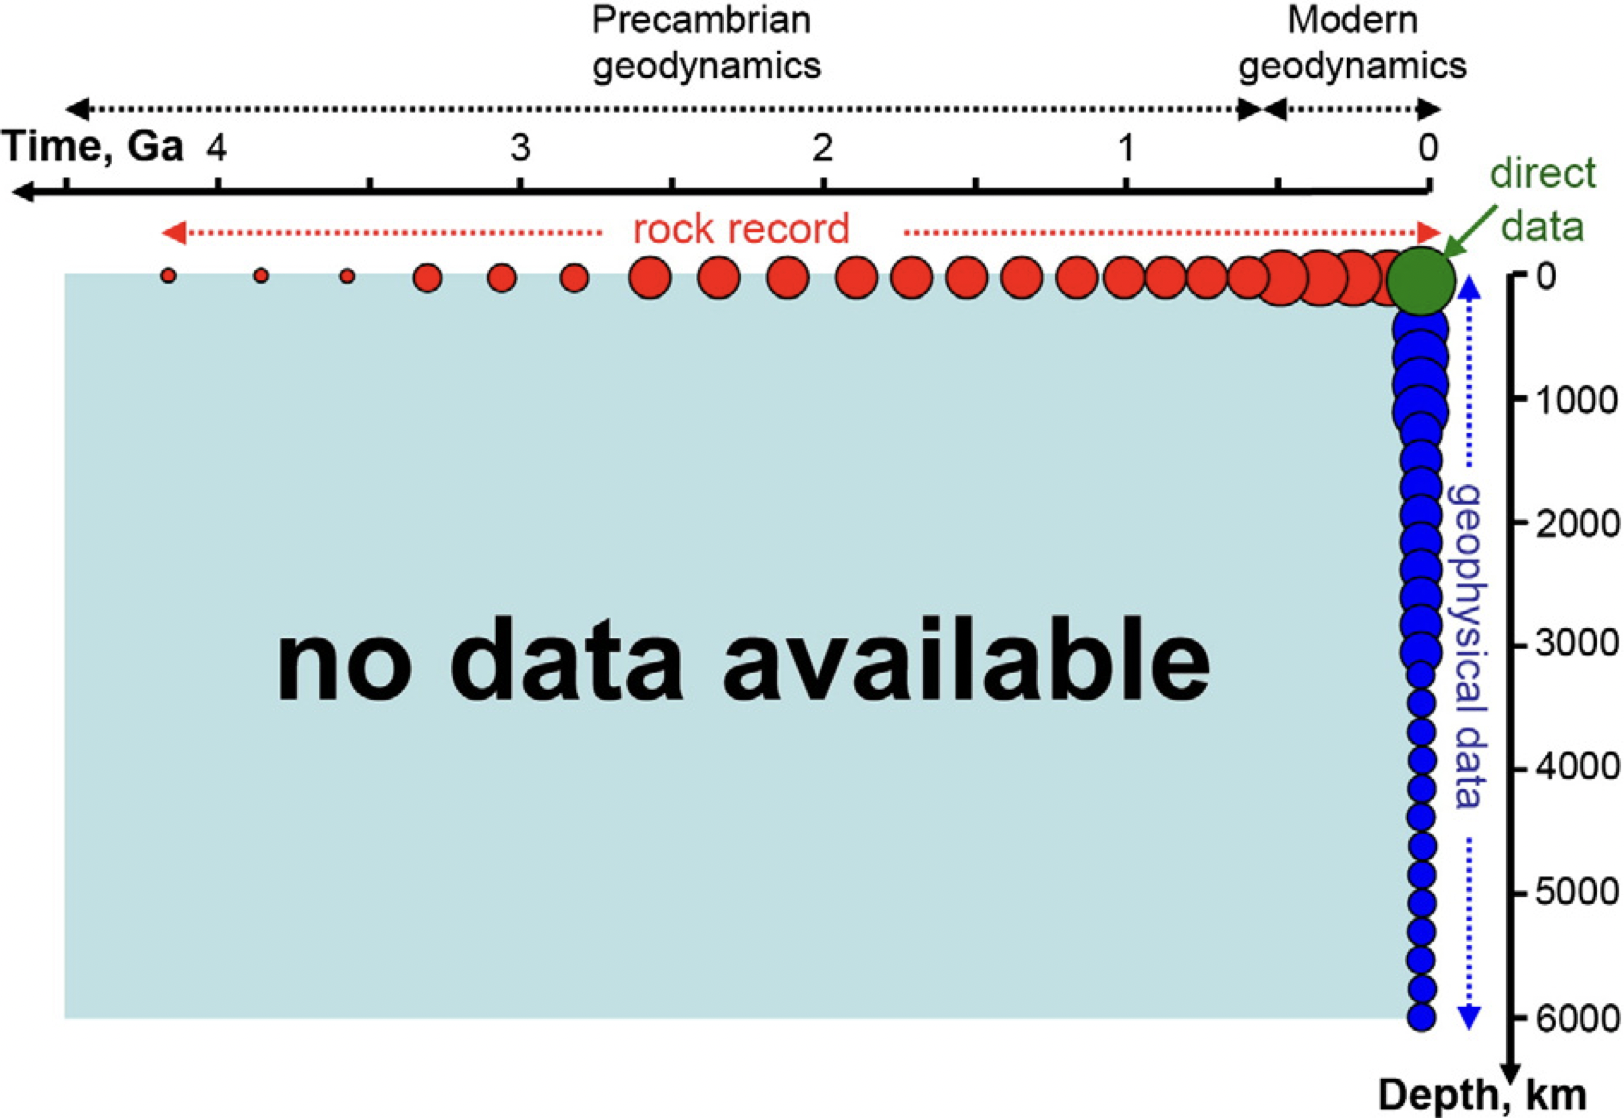
\includegraphics[width=1\linewidth,]{assets/figs/chpt1/gerya2014} 

}

\caption[The Geodynamicist's dilemma]{The Geodynamicist's dilemma. Time-depth diagram representing the data availability on Earth. The rock record (red circles) encodes information about geodynamic processes throughout Earth's history, but only within approximately 100 \(km\) of Earth's surface. Geophysical data (blue circles) provide images of Earth's deep interior, but only since the 20th century CE (or 10\(^{-7}\) \(Ga\)). Direct observations (green circle) are limited to the present-day surface. Size of the circles represents the abundance of available data. Reprinted from Gerya (\protect\hyperlink{ref-gerya2014}{2014}) with permission.}\label{fig:sparse}
\end{figure}

Subduction occurs when two lithospheric plates converge and the denser plate \emph{subducts} beneath the other at a \emph{subduction zone}. Subduction zones are implicated in myriad geodynamic phenomena, including seismicity, metamorphism, volatile flux, volcanism, dynamic plate motions, and crustal deformation (\protect\hyperlink{ref-cizkova2013}{Čížková \& Bina, 2013}; \protect\hyperlink{ref-gao2017}{Gao \& Wang, 2017}; \protect\hyperlink{ref-gonzalez2016}{Gonzalez et al., 2016}; \protect\hyperlink{ref-grove2012}{Grove et al., 2012}; \protect\hyperlink{ref-hacker2003}{Hacker et al., 2003}; \protect\hyperlink{ref-hirauchi2010}{Hirauchi et al., 2010}; \protect\hyperlink{ref-peacock1990}{Peacock, 1990}, \protect\hyperlink{ref-peacock1991}{1991}, \protect\hyperlink{ref-peacock1993}{1993}, \protect\hyperlink{ref-peacock1996}{1996}; \protect\hyperlink{ref-peacock1999a}{Peacock \& Hyndman, 1999}; \protect\hyperlink{ref-vankeken2011}{van Keken et al., 2011}). These phenomena are largely defined by plate motions and mechanical behavior along the plate interface (\protect\hyperlink{ref-furukawa1993}{Furukawa, 1993}; \protect\hyperlink{ref-peacock1994}{Peacock et al., 1994}; \protect\hyperlink{ref-peacock1996}{Peacock, 1996}). Important inputs and thermo-kinematic boundary conditions exerting first-order control on subduction zone structure and geodynamics (plate velocity, subduction angle, plate thickness, sediment thickness, crustal structure, subduction duration, and others) vary considerably among presently active subduction zones worldwide (e.g., \protect\hyperlink{ref-syracuse2010}{Syracuse et al., 2010}; \protect\hyperlink{ref-syracuse2006}{Syracuse \& Abers, 2006}).

Intuition suggests subduction zone inputs and thermo-kinematic boundary conditions should influence mechanical behavior along the plate interface. Yet previous work argues for rather uniform depths of plate (de)coupling among subduction zones with diverse thermo-kinematic boundary conditions (\protect\hyperlink{ref-furukawa1993}{Furukawa, 1993}; \protect\hyperlink{ref-wada2008}{Wada et al., 2008}; \protect\hyperlink{ref-wada2009}{Wada \& Wang, 2009}). Models based on such uniform mechanical behavior are widely adopted over alternative models (after \protect\hyperlink{ref-syracuse2010}{Syracuse et al., 2010}) and imply some aspects of subduction zone mechanics are minimally affected by thermo-kinematic boundary conditions. However, the spatial variability (with depth \emph{and} along strike in map view) of plate interface mechanics is difficult to quantify and currently characterized for transects across relatively few subduction zone segments compared to the global extent of actively converging margins.

This dissertation is motivated by the following question. How can one quantify the spatial variability of plate interface mechanical behavior across a range of subduction zones? Each chapter focuses on quantifying an aspect of subduction zone mechanics using different computational approaches and datasets.

Chapter \ref{chpt2} numerically simulates oceanic-continental subduction across a range of thermo-kinematic boundary conditions and plate coupling is observed after 10 \(Ma\). Multivariate linear regression is then used to formulate an expression for estimating coupling depth. The expression requires estimates for upper-plate thickness, which can be inverted from surface heat flow. Average upper-plate surface heat flow for 13 presently active subduction zones yield a narrow distribution of coupling depths---supporting the idea of broadly uniform mechanical coupling depths among subduction zones.

Chapter \ref{chpt3} takes a closer look surface heat flow by quantifying its spatial variability in 2D. Two interpolations methods, Kriging and Similarity, are compared to assess differences in their regional heat flow predictions near subduction zones. While Kriging and Similarity yield comparable regional interpolations on average, both approaches show lateral (along strike) surface heat flow variability in the upper plate. Discontinuous upper-plate surface heat flow implies non-uniform upper-plate thickness and contradicts broadly uniform coupling depths predicted in Chapter \ref{chpt2}.

Finally, Chapter \ref{chpt4} applies machine learning techniques to recognize detachment of subducting markers (representing recovered rock fragments) from the numerical simulations in Chapter \ref{chpt2}. A large (91,733) \glsfirst{ptt} dataset of recovered markers is compared across numerical experiments and with a global compilation of \gls{pt} estimates for rocks exhumed from subduction zones (the rock record). Marker \gls{ptt} distributions are distinct from the rock record for most numerical simulations, except for the most slowly-converging systems (40 \(km/Ma\)). Both marker \gls{ptt} distributions and marker recovery rates correlate with thermo-kinematic boundary conditions, implying non-uniform mechanical detachment of rock among subduction zones.

\cleardoublepage

\hypertarget{chpt2}{%
\chapter{Effects of Thermo-kinematic Boundary Conditions on Plate Coupling in Subduction Zones}\label{chpt2}}

\markboth{Chapter 2: Coupling Depths}{Chapter 2: Coupling Depths}

\DIFdelbegin %DIFDELCMD < \begin{quote}
%DIFDELCMD < %%%
\textbf{\DIFdel{Keypoints:}}
%DIFAUXCMD
%DIFDELCMD < 

%DIFDELCMD < \begin{itemize}
\begin{itemize}%DIFAUXCMD
%DIFDELCMD < \item
\item%DIFAUXCMD
%DIFDELCMD <   %%%
\DIFdel{Plate coupling responds strongly to upper-plate thickness
}%DIFDELCMD < \item
\item%DIFAUXCMD
%DIFDELCMD <   %%%
\DIFdel{Inverting surface heat flow allows coupling depth estimation
}%DIFDELCMD < \item
\item%DIFAUXCMD
%DIFDELCMD <   %%%
\DIFdel{Globally consistent surface heat flow implies consistent upper-plate thickness, and thus uniform coupling depths
}
\end{itemize}%DIFAUXCMD
%DIFDELCMD < \end{itemize}
%DIFDELCMD < \end{quote}
%DIFDELCMD < 

%DIFDELCMD < %%%
\DIFdelend \hypertarget{chpt2Abstract}{%
\section{Abstract}\label{chpt2Abstract}}

Deep mechanical coupling between converging plates is implicated in dynamic plate motions, crustal deformation, seismic cycles, arc magmatism, detachment (recovery) of subducting material, and is considered a key feature of subduction zone geodynamics. This study uses two-dimensional numerical simulations of oceanic-continental convergent margins to investigate effects of thermo-kinematic boundary conditions on coupling---specifically focusing on thermal parameter (\(\Phi\)) and upper-plate thickness. Numerical simulations implement coupling by including the metamorphic (de)hydration reaction \(antigorite \allowbreak \Leftrightarrow olivine + orthopyroxene + H_{2}O\) in the upper-plate mantle. Visualizing P-T-strain fields show thermal feedbacks regulating coupling depth dynamically with strong responses to upper-plate thickness and weak responses to \(\Phi\). The results imply estimation of coupling depth is possible by inverting upper-plate thickness from surface heat flow. Moreover, surface heat flow sampled from the backarc region near 17 presently active subduction zones imply uniform upper-plate thickness, and thus uniform coupling depths among subduction zones.

\hypertarget{chpt2Intro}{%
\section{Introduction}\label{chpt2Intro}}

Subduction geodynamics are largely defined by plate motions and mechanical behavior along the plate interface. For example, a transition from mechanically decoupled (plates moving differentially with respect to each other) to coupled plates (plates moving with the same local velocity) dramatically increases temperature by inducing mantle circulation in the upper-plate asthenospheric mantle (\protect\hyperlink{ref-peacock1994}{Peacock et al., 1994}; \protect\hyperlink{ref-peacock1996}{Peacock, 1996}). Observations from numerical simulations and forearc surface heat flow imply coupling transitions occur globally within a narrow range of depths in modern subduction zones (70-80 \(km\)). Further, coupling appears essentially unresponsive to diverse thermo-kinematic boundary conditions, including oceanic-plate age, convergence velocity, and subduction geometry (\protect\hyperlink{ref-furukawa1993}{Furukawa, 1993}; \protect\hyperlink{ref-wada2008}{Wada et al., 2008}; \protect\hyperlink{ref-wada2009}{Wada \& Wang, 2009}). While uniform coupling depths among subduction zones are inferred from numerical simulations and surface heat flow, this phenomenon remains curious and unconfirmed to a large extent. To understand subduction zone geodynamics, it is essential to understand why modern subduction zones appear to achieve similar coupling depths despite differences in their physical characteristics.

Notwithstanding, many numerical geodynamic models use coupling depths of 70-80 \(km\) as a boundary condition (\protect\hyperlink{ref-abers2017}{Abers et al., 2017}; \protect\hyperlink{ref-currie2004}{Currie et al., 2004}; \protect\hyperlink{ref-gao2014}{Gao \& Wang, 2014}; \protect\hyperlink{ref-syracuse2010}{Syracuse et al., 2010}; \protect\hyperlink{ref-vankeken2011}{van Keken et al., 2011}, \protect\hyperlink{ref-vankeken2018}{2018}; \protect\hyperlink{ref-wada2012}{Wada et al., 2012}; \protect\hyperlink{ref-wilson2014}{Wilson et al., 2014}), although not exclusively (e.g.~40-56 \(km\), \protect\hyperlink{ref-england2010}{England \& Katz, 2010}; \protect\hyperlink{ref-peacock1996}{Peacock, 1996}). Similar coupling depths among subduction zones is an attractive hypothesis for at least two reasons. First, it helps explain a relatively narrow range of depths to subducting oceanic-plates beneath volcanic arcs (\protect\hyperlink{ref-england2004}{England et al., 2004}; \protect\hyperlink{ref-syracuse2006}{Syracuse \& Abers, 2006}) as mechanical coupling is expected to be closely associated with the onset of flux melting. Second, mechanical coupling is required to detach crustal fragments from the subducting plate (\protect\hyperlink{ref-agard2016}{Agard et al., 2016}), so uniform coupling depths may also help explain why maximum pressures recorded by subducted oceanic material worldwide is \(\leq\) 2.3-2.5 \(GPa\) (roughly 80 \(km\), \protect\hyperlink{ref-agard2009}{Agard et al., 2009}, \protect\hyperlink{ref-agard2018}{2018}).

The location and extent of mechanical coupling along the plate interface is implicated in myriad geodynamic phenomena, including seismicity, metamorphism, volatile flux, volcanism, plate motions, and crustal deformation (\protect\hyperlink{ref-cizkova2013}{Čížková \& Bina, 2013}; \protect\hyperlink{ref-gao2017}{Gao \& Wang, 2017}; \protect\hyperlink{ref-gonzalez2016}{Gonzalez et al., 2016}; \protect\hyperlink{ref-grove2012}{Grove et al., 2012}; \protect\hyperlink{ref-hacker2003}{Hacker et al., 2003}; \protect\hyperlink{ref-hirauchi2010}{Hirauchi et al., 2010}; \protect\hyperlink{ref-peacock1990}{Peacock, 1990}, \protect\hyperlink{ref-peacock1991}{1991}, \protect\hyperlink{ref-peacock1993}{1993}, \protect\hyperlink{ref-peacock1996}{1996}; \protect\hyperlink{ref-peacock1999a}{Peacock \& Hyndman, 1999}; \protect\hyperlink{ref-vankeken2011}{van Keken et al., 2011}). Consequently, the mechanics of coupling have been extensively studied and discussed. Coupling fundamentally depends on the strength (viscosity) of materials above, within, and below the plate interface. Water flux from compaction and dehydration of hydrous minerals with increasing \glsfirst{pt} forms layers of low viscosity sheet silicates near the plate interface. Transmission of shear stress between plates is inhibited by formation of talc and serpentine in the shallow upper-plate mantle (\protect\hyperlink{ref-peacock1999a}{Peacock \& Hyndman, 1999}). Lack of traction along the interface, combined with cooling from the subducting plate surface, ensures a positive feedback between hydrous mineral formation and mechanical decoupling. Experimentally determined flow laws, petrologic observations, and geophysical observations all support the plausibility of this conceptual model of subduction interface behavior (e.g., \protect\hyperlink{ref-agard2016}{Agard et al., 2016}, \protect\hyperlink{ref-agard2018}{2018}; \protect\hyperlink{ref-gao2014}{Gao \& Wang, 2014}; \protect\hyperlink{ref-peacock1999a}{Peacock \& Hyndman, 1999}).

Experimental control over important thermo-kinematic boundary conditions make geodynamic numerical simulations essential for investigating such complex geodynamic environments. Wada \& Wang (\protect\hyperlink{ref-wada2009}{2009}) previously investigated the effects of \(\Phi\) on coupling depths by numerically simulating 17 presently active subduction zones. Among other thermo-kinematic boundary conditions, their models specify convergence rate, subduction geometry, thermal structure of oceanic- and overriding-plates, and degree of coupling along the subduction interface. Notably, their experiments control for interface rheology and discriminate best-fit coupling depths based on observed forearc surface heat flow.

This study similarly specifies thermo-kinematic boundary conditions to numerically simulate the range of modern subduction zone systems, but regulates interface rheology dynamically by implementing metamorphic reactions that respond to evolving P-T-strain fields. Subduction geometry and coupling depth are not fully determined features, in other words, but spontaneous model outcomes within the range of specified boundary conditions discussed in Section \ref{numMethods}. As in previous studies (e.g., \protect\hyperlink{ref-ruh2015}{Ruh et al., 2015}), rheological effects of the dehydration reaction \(antigorite \allowbreak \Leftrightarrow olivine + orthopyroxene + H_{2}O\) are implemented to drive mechanical coupling. An abrupt viscosity increase accompanies antigorite (serpentine) destabilization, thereby inducing mechanical coupling, as defined by empirically-determined flow laws used in the experiments (Table \ref{tab:materials}).

This chapter focuses on two fundamental questions. How does coupling depth respond to \(\Phi\) \emph{and} upper-plate thickness? And how stable is coupling depth through time? First, 64 convergent margins with variable upper-plate thickness and \(\Phi\) are numerically simulated and mechanical plate coupling is observed. Thermal feedbacks within the system are visualized in terms of mantle temperature, viscosity, and velocity fields and coupling depth responses to a range of \(\Phi\) and upper-plate thickness are quantified using multivariate linear regression. Three different regression models are then used to estimate coupling depths for 17 presently active subduction zones. Coupling depth estimates are narrowly distributed, regardless of regression model form. Finally, implications and questions regarding uniformity among subduction zones in terms of surface heat flow, upper-plate thickness, and coupling depth are discussed.

\hypertarget{numMethods}{%
\section{Numerical Modelling Methods}\label{numMethods}}

This study simulates converging oceanic-continental plates, where an ocean basin is being consumed by subduction at a continental margin (Figure \ref{fig:init}). Initial conditions are modified from previous numerical experiments of active margins (\protect\hyperlink{ref-gorczyk2007}{Gorczyk et al., 2007}; \protect\hyperlink{ref-sizova2010}{Sizova et al., 2010}) using the code \texttt{I2VIS} (\protect\hyperlink{ref-gerya2003}{Gerya \& Yuen, 2003}), although plate coupling was not the focus of their studies. An identical rheologic model with identical material properties (Table \ref{tab:materials}), and a identical hydration/melt model (Table \ref{tab:melts} \& Appendix \ref{deHydration}) to Sizova et al. (\protect\hyperlink{ref-sizova2010}{2010}) are implemented. However, the version of \texttt{I2VIS} in this study differs from Sizova et al. (\protect\hyperlink{ref-sizova2010}{2010}) in its initial setup, overall dimension, resolution, continental geotherm, dehydration model, and left boundary condition (origin of new oceanic lithosphere). Differences are outlined in this section and in Appendix \ref{deHydration}. Sixty-four \texttt{I2VIS} models constructed with varying convergence rates (\(\vec{v}\)), oceanic-plate ages, and upper-plate thickness (Figure \ref{fig:params}) were ran on the \href{https://scicomp.ethz.ch/wiki/Euler}{Euler cluster} at ETH, Zürich for at least 100 timesteps.

\begin{landscape}


\begin{figure}[htbp]

{\centering 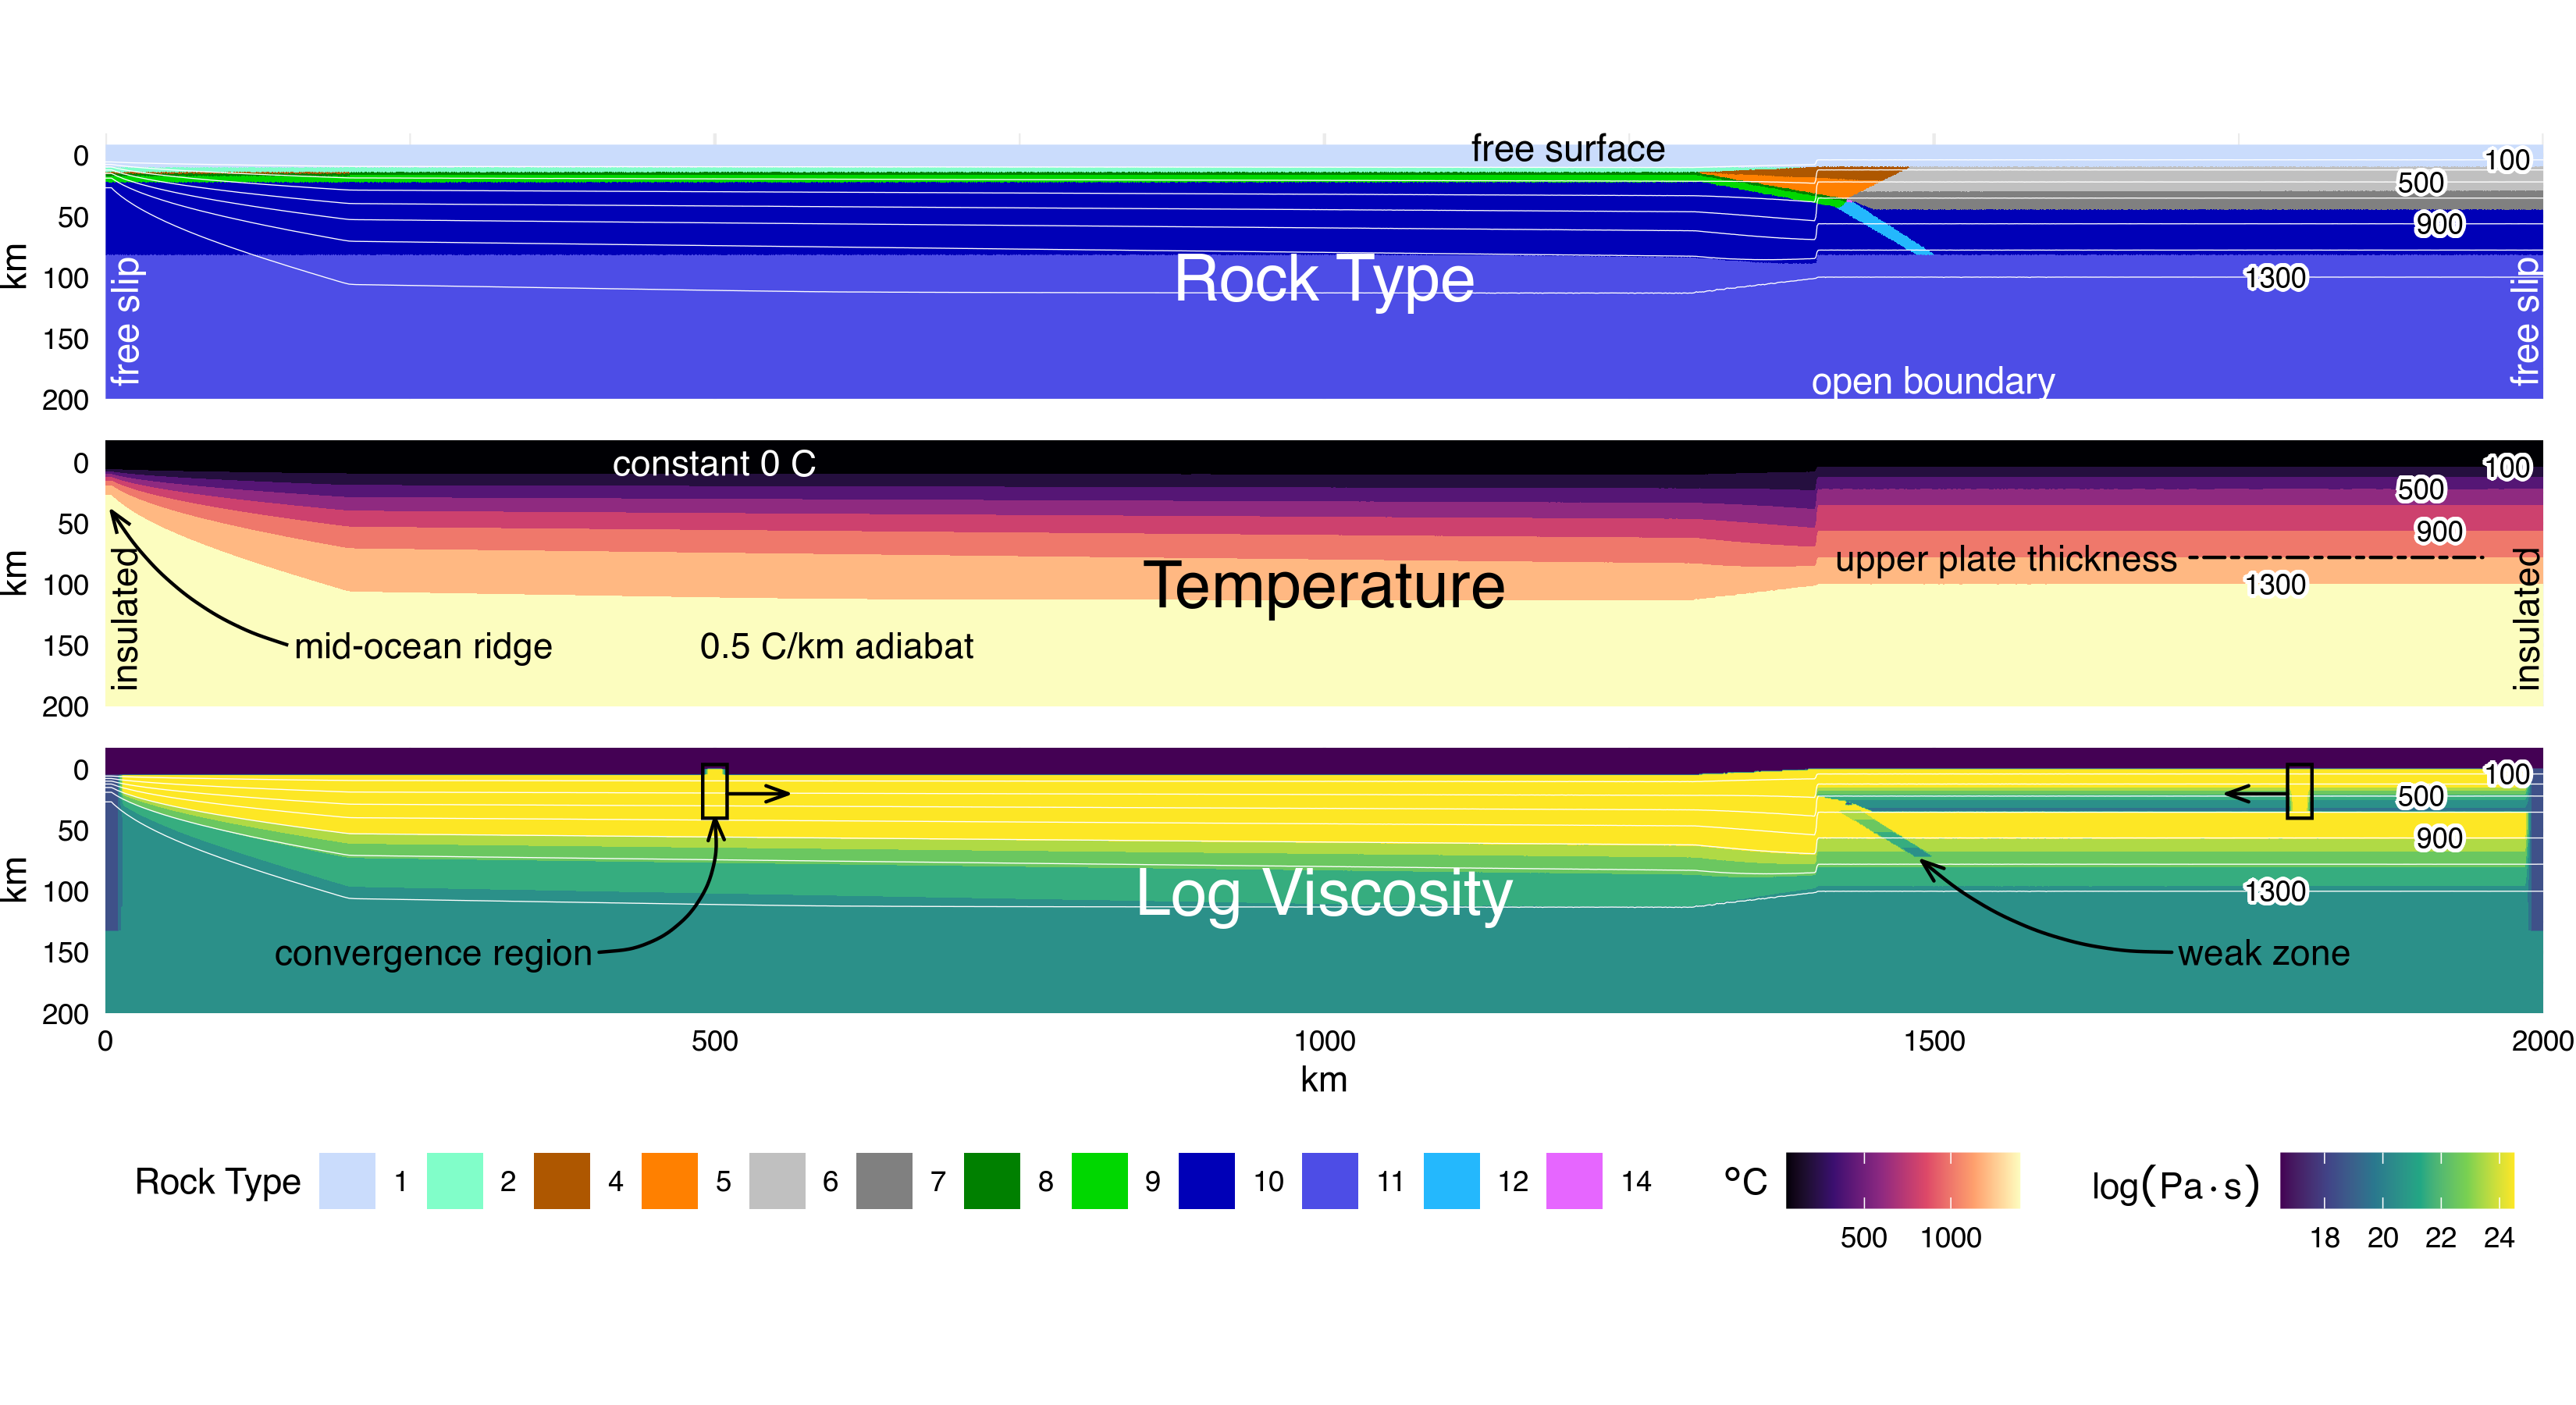
\includegraphics[width=1\linewidth,]{assets/figs/chpt2/fig1} 

}

\caption[Initial model configuration and boundary conditions]{Initial model configuration and boundary conditions. (a) A free sedimentation/erosion boundary at the surface is maintained by implementing a layer of "sticky" air and water, and an infinite-like open boundary at the bottom allows for spontaneous oceanic-plate descent and subduction angle. Left and right boundaries are free slip and thermally insulating. Initial material distribution includes 7 $km$ of oceanic crust (2 $km$ basalt, 5 $km$ gabbro), 1 $km$ of oceanic sediments, and 35 $km$ of continental crust, thinning ocean-ward. (b) Oceanic lithosphere is continually created at the left boundary. The oceanic geotherm is calculated using a half-space cooling model and the continental geotherm is calculated using a one-dimensional steady-state conductive cooling model to 1300 $^{\circ}C$. The base of the upper-plate lithosphere ($Z_{UP}$) is defined by visualizing viscosity and generally coincides with the 1100 $^{\circ}C$ isotherm. (c) Oceanic crust is bent under loading from passive margin sediments, and a weak zone extends through the lithosphere to help induce subduction. Convergence velocities are imposed at stationary, high-viscosity regions far from the trench. Rock type colors are: [1] air, [2] water, [4,5] sediments, [6,7] felsic crust, [8] basalt, [9] gabbro, [10,11] dry mantle, [12] hydrated mantle, [14] serpentinized mantle.}\label{fig:init}
\end{figure}


\end{landscape}

\hypertarget{numBCs}{%
\subsection{Initial Setup and Boundary Conditions}\label{numBCs}}

Simulations are 2000 \(km\) wide and 300 \(km\) deep (Figure \ref{fig:init}). In the model domain, three governing equations of heat transport, momentum, and continuity are discretized and solved with a conservative finite-difference marker-in-cell approach on a fully staggered grid as outlined in Gerya \& Yuen (\protect\hyperlink{ref-gerya2003}{2003}). Numerical resolution is non-uniform with higher resolution (1 \(km\) x 1 \(km\)) in a 600 \(km\) wide area surrounding the contact between the oceanic-plate and continental margin, then gradually changing to lower resolution towards the model boundaries (5 \(km\) x 1 \(km\), x- and z-directions, respectively). The left and right boundaries are free-slip and thermally insulating (Figure \ref{fig:init}a, b). Implementation of ``sticky'' air and water allows for a free topographical surface with a simple linear sedimentation and erosion model. The lower boundary is open to allow for oceanic-plate descent with a spontaneous subduction angle (\protect\hyperlink{ref-burg2005}{Burg \& Gerya, 2005}).

A horizontal convergence force is applied to both plates in a rectangular region far from the continental margin (Figure \ref{fig:init}c). An initial weak layer cutting the lithosphere permits subduction to initiate. The high-viscosity (\(\eta = 10^{25}~Pa\cdot s\)) rectangular convergence regions apply constant horizontal velocities without deforming the lithosphere. Subduction angle is governed by free-motion of the subducting plate. Similarly, subduction velocity varies with time in response to extension or shortening of the overriding plate. \(\Phi\) is thus calculated as the product of the horizontal convergence velocity and the oceanic-plate age (c.f. \protect\hyperlink{ref-kirby1991}{Kirby et al., 1991}; \protect\hyperlink{ref-mckenzie1969}{McKenzie, 1969}). For convenience and consistency with the literature, this study presents \(\Phi\) in units of \(km\)/100 (Figure \ref{fig:params}a).

\begin{figure}[htbp]

{\centering 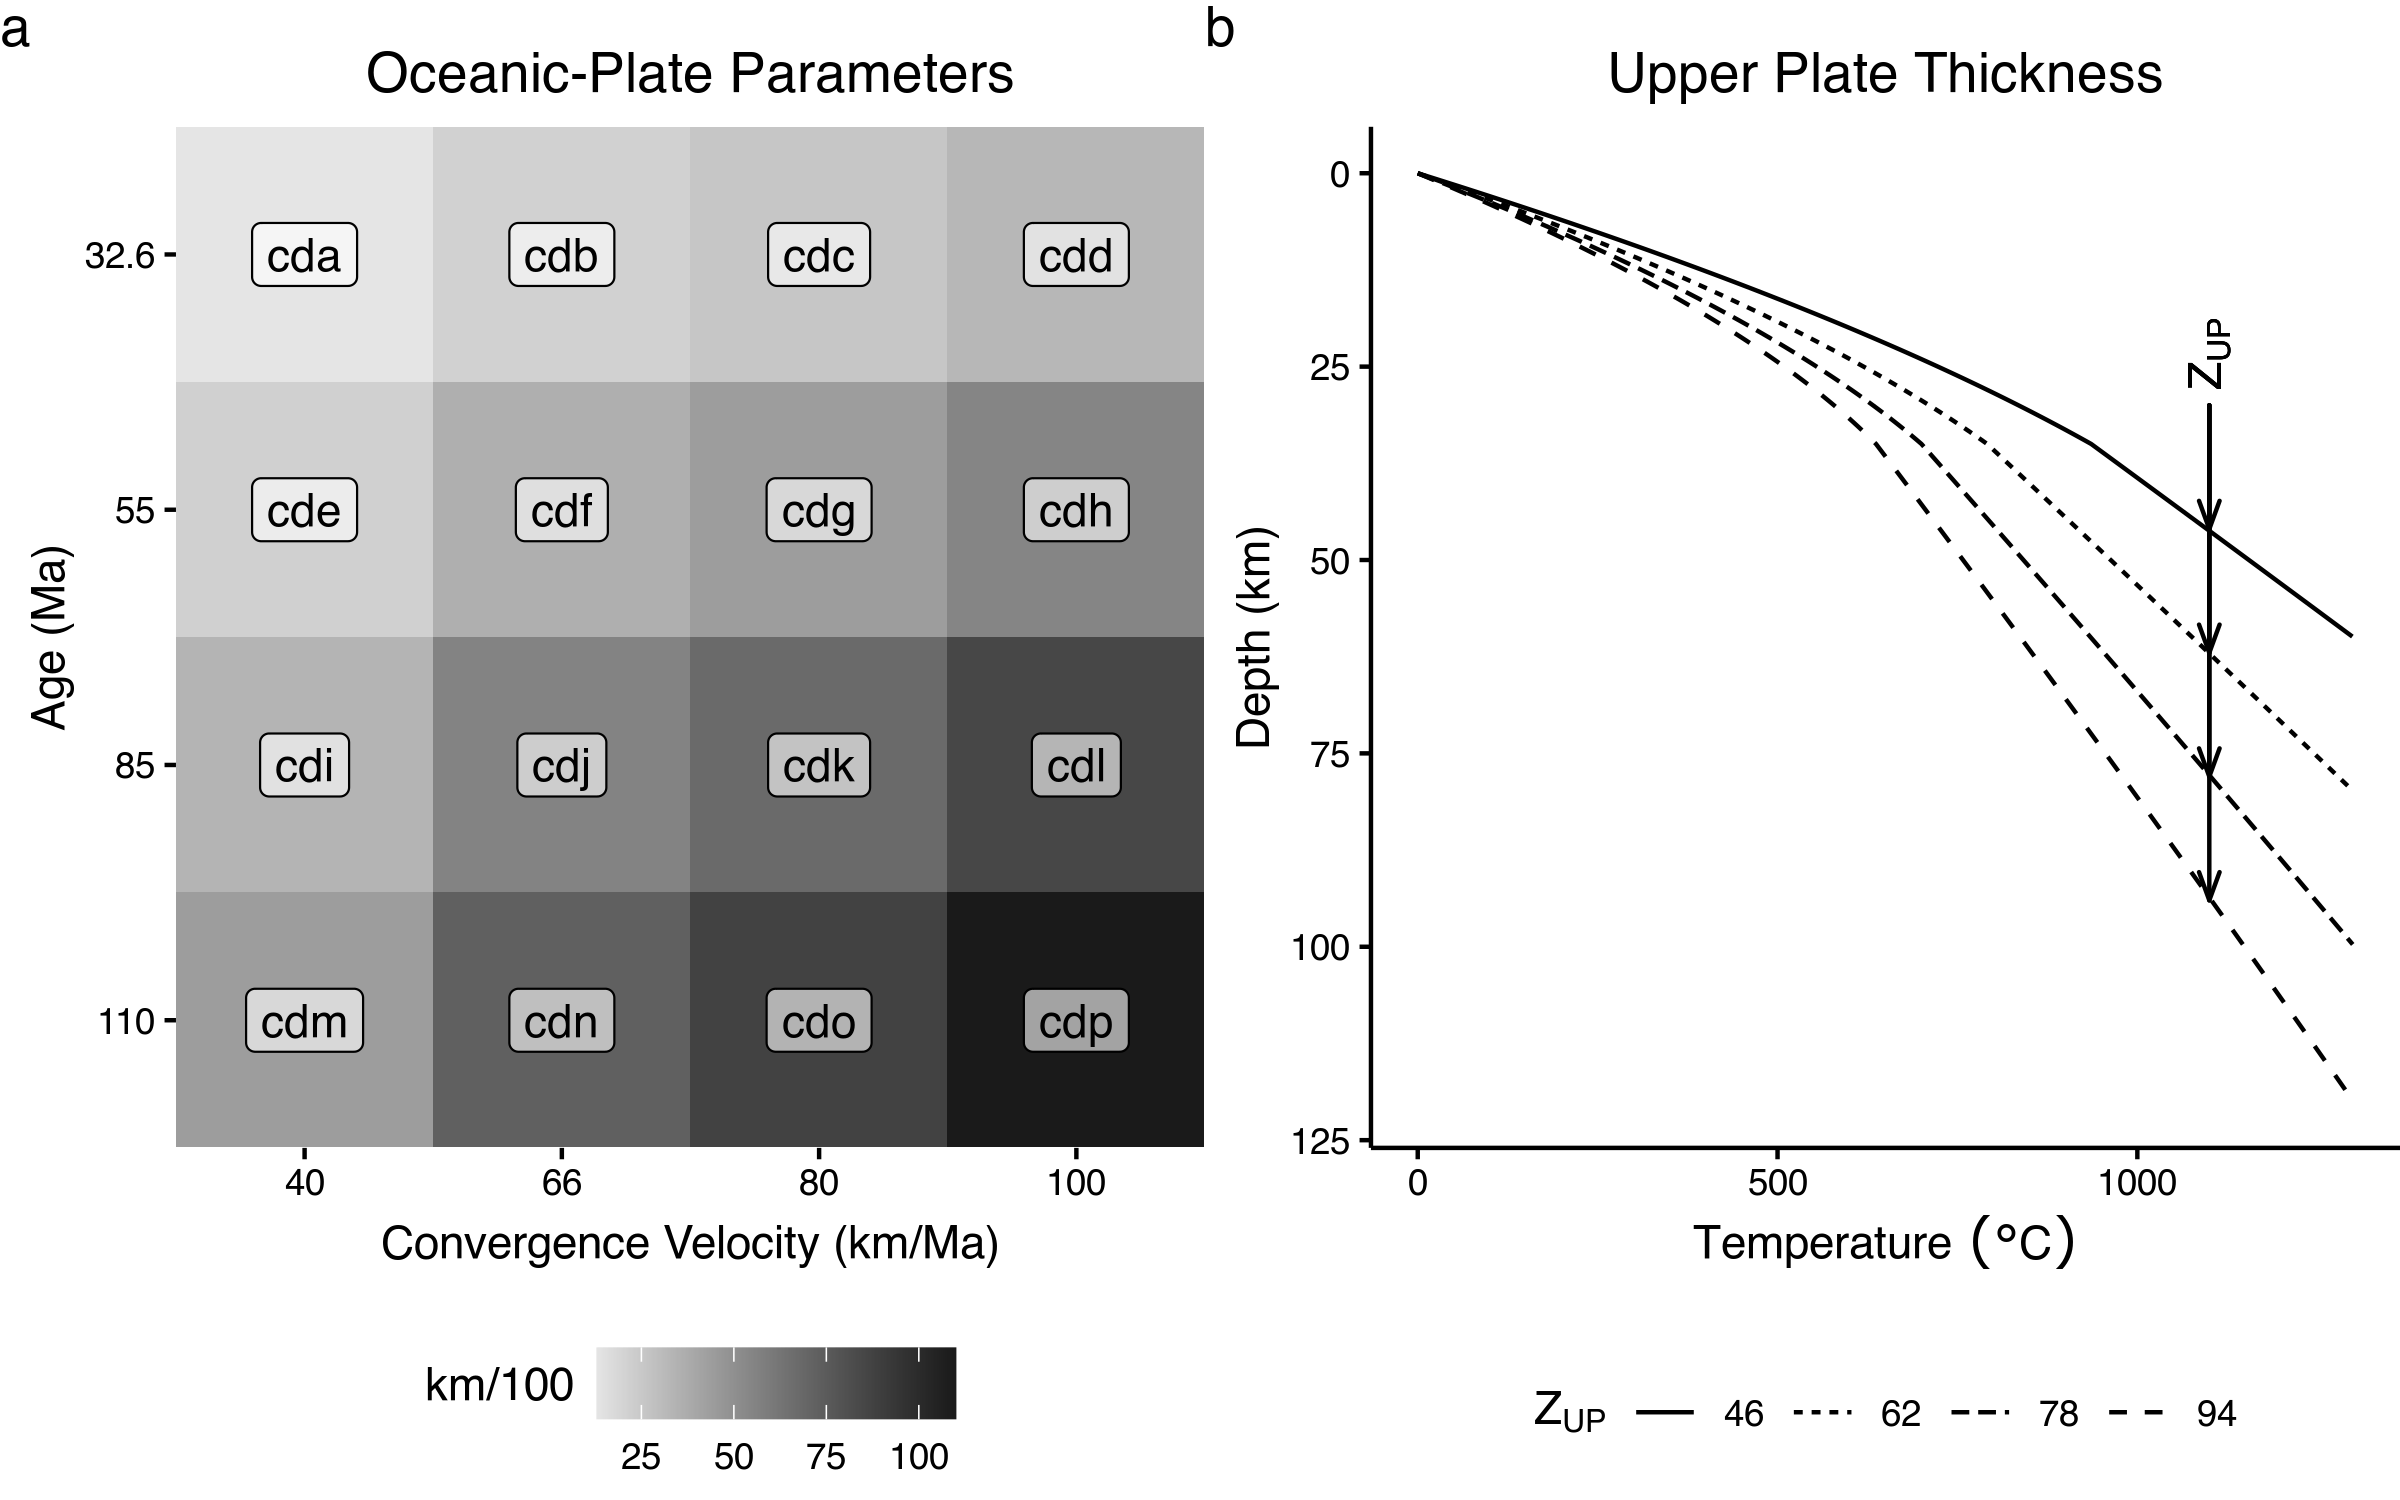
\includegraphics[width=1\linewidth,]{assets/figs/chpt2/fig2} 

}

\caption[Range of boundary conditions used in numerical experiments]{Range of thermo-kinematic boundary conditions used in numerical experiments. (a) Thermal parameters (grayscale) range from 13 to 110 $km/100$ and broadly reflect the distribution of oceanic-plate ages and convergence velocities in modern subduction zones. Model names include the prefix "cd" for "coupling depth" with increasing alphabetic suffixes. Note that neither axes are continuous. (b) Upper-plate thickness ($Z_{UP}$) is defined by a range of continental geotherms. Geotherms were constructed using a one-dimensional steady-state conductive cooling model with $T(z=0)$ = 0 $^{\circ}C$, $\vec{q}(z=0)$ = 59, 63, 69, 79 $mW/m^2$, and constant radiogenic heating of 1.0 $\mu W/m^3$ for a 35 $km$-thick crust and 0.022 $\mu W/m^3$ for the mantle. Continental geotherms are calculated up to 1300 $^{\circ}$C with a constant 0.5 $^{\circ}C/km$ gradient (the mantle adiabat) extending to the base of the model domain.}\label{fig:params}
\end{figure}

\hypertarget{numGeotherms}{%
\subsection{Defining Geotherms and Lithospheric Thickness}\label{numGeotherms}}

Oceanic crust is modeled as 1 \(km\) of sediment cover overlying 2 \(km\) of basalt and 5 \(km\) of gabbro (Figure \ref{fig:init}a). Oceanic lithosphere is continually made at a pseudo-mid-ocean ridge at the left boundary of the model (Figure \ref{fig:init}b). An enhanced vertical cooling condition applied at 200 \(km\) from left boundary adjusts for the proper oceanic-plate age, and therefore its lithospheric thickness as it enters the trench (\protect\hyperlink{ref-agrusta2013}{Agrusta et al., 2013}). Oceanic-plate ages range from 32.6 to 110 \(Ma\) and convergence velocities from 40 to 100 \(km/Ma\) (Figure \ref{fig:params}a). This range of parameters broadly reflects the middle-range of modern global subduction systems (\protect\hyperlink{ref-syracuse2006}{Syracuse \& Abers, 2006}).

Initial continental geotherms are determined by solving the heat flow equation in one-dimension to 1300 \(^{\circ}C\) (Figure \ref{fig:params}b). This study assumes a fixed temperature of 0 \(^{\circ}C\) at the surface, constant radiogenic heating of 1 \(\mu W/m^{3}\) in the 35 \(km\)-thick continental crust, 0.022 \(\mu W/m^{3}\) in the mantle, with thermal conductivities of 2.3 \(W/mK\) and 3.0 \(W/mK\) for the continental crust and mantle, respectively. Above, 1300 \(^{\circ}C\), temperature is assumed to constantly increase by 0.5 \(^{\circ}C/km\) (the mantle adiabat) to the base of the model domain.

Many studies define the base of the continental lithosphere at the 1300 \(^{\circ}C\) isotherm, but it can be determined directly by visualizing viscosity and strain rate as the model progresses. The mechanical base of the lithosphere (\(Z_{UP}\)) in the models generally occurs near the 1100 \(^{\circ}C\) isotherm---characterized by a rapid decrease in viscosity and increase in strain rate (Figures \ref{fig:cdfStep1}, \ref{fig:cdfStep2}, \ref{fig:cdfStep3}). As such, this study considers oceanic and continental lithospheres as mechanical layers defined by viscosity, rather than defined merely by temperature. \(Z_{UP}\) corresponding to backarc surface heat flow of 59, 63, 69, and 79 \(mW/m^{2}\) are used in this study (Figure \ref{fig:params}b).

\hypertarget{numHydration}{%
\subsection{Metamorphic (De)hydration Reactions}\label{numHydration}}

Using Lagrangian markers (\protect\hyperlink{ref-harlow1962}{Harlow, 1962}, \protect\hyperlink{ref-harlow1964}{1964}) to store and update material properties and P-T-strain fields allows for straight-forward numerical implementation of metamorphic reactions. This approach is key to regulating mechanical coupling dynamically in subduction zone simulations. For example, dehydration (eclogitization) of the oceanic-plate and (de)stabilization of serpentine in the upper-plate mantle may be effectively modelled by tracing marker \gls{ptt} paths while changing marker properties according to thermodynamically-stable mineral assemblages (e.g., \protect\hyperlink{ref-connolly2005}{Connolly, 2005}). For computational efficiency, however, water contents in this study are not computed by iteratively solving thermodynamic systems of equations. Instead, gradual eclogitization of oceanic crust is computed as a linear function of lithostatic pressure to a maximum depth of 150 \(km\), or temperature of 1427 \(^\circ C\), while including garnet-in and plagioclase-out reactions defined by Ito \& Kennedy (\protect\hyperlink{ref-ito1971}{1971}). Mantle (de)hydration is computed according reactions boundaries defined by Schmidt \& Poli (\protect\hyperlink{ref-schmidt1998}{1998}) with a maximum water content of 2 \(wt.\%\) (explained below). This approach effectively simulates continuous influx of water to the upper-plate mantle with relatively low computational cost, beginning with compaction and release of connate water at shallow depths, followed by a sequence of reactions consuming major hydrous phases (chlorite, lawsonite, zoisite, chloritoid, talc, amphibole, and phengite) in different parts of the hydrated basaltic crust (\protect\hyperlink{ref-schmidt1998}{Schmidt \& Poli, 1998}; \protect\hyperlink{ref-vankeken2011}{van Keken et al., 2011}).

The extent of metamorphic reaction effects on mechanical coupling, and the exact (de)hydration reaction(s) likely responsible, are unknown. However, formation of brucite and serpentine from dry olivine near the plate interface are inferred to strongly regulate mechanical behavior (\protect\hyperlink{ref-agard2016}{Agard et al., 2016}; \protect\hyperlink{ref-hyndman2003}{Hyndman \& Peacock, 2003}; \protect\hyperlink{ref-peacock1999a}{Peacock \& Hyndman, 1999}). Brucite notably breaks down at much lower temperatures than serpentine (\protect\hyperlink{ref-schmidt1998}{Schmidt \& Poli, 1998}), so serpentine (de)stabilization arguably represents the key transition from a weak-to-strong upper-plate mantle deep in subduction zones. This study elects an implementation of serpentine (de)hydration for this reason. The reaction is assumed to be abrupt and discontinuous, which is a fine approximation for near-endmember compositions like (Mg-rich) peridotites. The \gls{pt} conditions of the reaction \(antigorite \Leftrightarrow olivine + orthopyroxene + H_{2}O\) were numerically implemented by the following equation (after \protect\hyperlink{ref-schmidt1998}{Schmidt \& Poli, 1998}):
\DIFdelbegin %DIFDELCMD < 

%DIFDELCMD < %%%
\DIFdelend \begin{equation}
  T_{atg-out}(z)=
  \begin{cases}
    751.50+6.008\times10^{-3}z-3.469\times10^{-8}z^2,& \text{for } z < 63000m \\
    1013.2-6.039\times10^{-5}z-4.289\times10{-9}z^2,& \text{for } z>63000m
  \end{cases}
  \label{eq:antstab}
\end{equation}
\DIFdelbegin %DIFDELCMD < 

%DIFDELCMD < %%%
\DIFdelend where \(z\) is the depth of a marker from the surface in meters and \(T\) is temperature in Kelvins. This reaction boundary is consistent to within 25 \(^{\circ}C\) of more recent experiments by Shen et al. (\protect\hyperlink{ref-shen2015}{2015}). Markers with internal temperature exceeding \(T_{atg-out}(z)\) spontaneously form \(olivine + orthopyroxene + H_{2}O\) and release their crystal-bound water. This implementation tacitly assumes thermodynamic equilibrium and is common to many versions of \texttt{I2VIS}.

Oceanic-plates of different ages are also tacitly assumed to dehydrate similarly with the above implementation. However, older (colder) oceanic-plates are expected to carry water to greater depths than younger (warmer) plates because of relatively delayed water-releasing reactions (\protect\hyperlink{ref-peacock1996}{Peacock, 1996}). Abrupt water release with serpentine dehydration (Equation \eqref{eq:antstab}) was tested to model deep water retention in cold oceanic-plates. Mechanical coupling behavior was indistinguishable from gradual water release models. This implies rates of water release are less important than the depth of serpentine stability. Explicitly modelling other major dehydration reactions are thus unlikely to significantly affect mechanical coupling behavior, yet likely to introduce numerical artifacts at great computational cost. A simplified gradual water release model for all oceanic-plates is therefore preferred.

Water released by rock forms discrete fluid particles that migrate with relative velocities defined by local deviatoric (non-lithostatic) pressure gradients (see Appendix \ref{deHydration}, \protect\hyperlink{ref-faccenda2009}{Faccenda et al., 2009}). Fluid velocities are scaled by a 10 \(cm/yr\) vertical percolation velocity to account for purely lithostatic pressure gradients in the mantle (\protect\hyperlink{ref-gorczyk2007}{Gorczyk et al., 2007}). Fluid particles migrate until encountering rock that can consume additional water by equilibrium hydration or melting reactions, (Equation \ref{tab:melts}).

The shallow upper-plate mantle can theoretically store large amounts of water as serpentine may contain up to 13 \(wt.\%\) water (\protect\hyperlink{ref-reynard2013}{Reynard, 2013}) and is generally stable at shallow mantle conditions. Thermodynamic models predict 8 \(wt.\%\) water in the shallow upper-plate mantle (\protect\hyperlink{ref-connolly2005}{Connolly, 2005}). However, seismic studies suggest most shallow upper-plate mantles are only partially serpentinized (\textless{} 20-40\%), equating to water contents of approximately 3-6 \(wt.\%\) (\protect\hyperlink{ref-abers2017}{Abers et al., 2017}; \protect\hyperlink{ref-carlson2003}{Carlson \& Miller, 2003}). Many modes of mantle hydration are documented or inferred, including evidence for channelized fluid flow within ophiolites exhumed from subduction zones (\protect\hyperlink{ref-angiboust2012a}{Angiboust et al., 2012a}, \protect\hyperlink{ref-angiboust2014}{2014}; \protect\hyperlink{ref-plumper2017}{Plümper et al., 2017}; \protect\hyperlink{ref-zack2007}{Zack \& John, 2007}). This study limits mantle wedge hydration to \(\leq\) 2 \(wt.\%~H_{2}O\) and assumes any excess \(H_{2}O\) exits the system through channelized fluid flow during plastic or brittle deformation (\protect\hyperlink{ref-davies1999}{Davies, 1999}).

\DIFaddbegin \begin{landscape}\DIFaddend \begin{table}

\caption{\label{tab:materials}Material properties used in numerical experiments}
\centering
\resizebox{\linewidth}{!}{
\begin{threeparttable}
\begin{tabular}[t]{lrrlrrrrrrrrlr}
\toprule
Material & $\rho$ & $H_2O$ & Flow Law & $log_{10}A$ & $E$ & $V$ & $n$ & $\phi$ & $\sigma_{crit}$ & $k_1$ & $k_2$ & $k_3$ & $H$\\
\midrule
\cellcolor{gray!6}{sediments} & \cellcolor{gray!6}{2600} & \cellcolor{gray!6}{5.0} & \cellcolor{gray!6}{wet quartzite} & \cellcolor{gray!6}{-3.5} & \cellcolor{gray!6}{154.0} & \cellcolor{gray!6}{3.0} & \cellcolor{gray!6}{2.3} & \cellcolor{gray!6}{0.15} & \cellcolor{gray!6}{0.03} & \cellcolor{gray!6}{0.64} & \cellcolor{gray!6}{807} & \cellcolor{gray!6}{4e-06} & \cellcolor{gray!6}{2.000}\\
felsic crust & 2700 &  & wet quartzite & -3.5 & 154.0 & 3.0 & 2.3 & 0.45 & 0.03 & 0.64 & 807 & 4e-06 & 1.000\\
\cellcolor{gray!6}{basalt} & \cellcolor{gray!6}{3000} & \cellcolor{gray!6}{5.0} & \cellcolor{gray!6}{plag an75} & \cellcolor{gray!6}{-3.5} & \cellcolor{gray!6}{238.0} & \cellcolor{gray!6}{8.0} & \cellcolor{gray!6}{3.2} & \cellcolor{gray!6}{0.45} & \cellcolor{gray!6}{0.03} & \cellcolor{gray!6}{1.18} & \cellcolor{gray!6}{474} & \cellcolor{gray!6}{4e-06} & \cellcolor{gray!6}{0.250}\\
gabbro & 3000 &  & plag an75 & -3.5 & 238.0 & 8.0 & 3.2 & 0.45 & 0.03 & 1.18 & 474 & 4e-06 & 0.250\\
\cellcolor{gray!6}{mantle dry} & \cellcolor{gray!6}{3300} & \cellcolor{gray!6}{} & \cellcolor{gray!6}{dry olivine} & \cellcolor{gray!6}{4.4} & \cellcolor{gray!6}{540.0} & \cellcolor{gray!6}{20.0} & \cellcolor{gray!6}{3.5} & \cellcolor{gray!6}{0.45} & \cellcolor{gray!6}{0.30} & \cellcolor{gray!6}{0.73} & \cellcolor{gray!6}{1293} & \cellcolor{gray!6}{4e-06} & \cellcolor{gray!6}{0.022}\\
mantle hydrated & 3300 & 0.5 & wet olivine & 3.3 & 430.0 & 10.0 & 3.0 & 0.45 & 0.24 & 0.73 & 1293 & 4e-06 & 0.022\\
\cellcolor{gray!6}{serpentine} & \cellcolor{gray!6}{3200} & \cellcolor{gray!6}{2.0} & \cellcolor{gray!6}{serpentine} & \cellcolor{gray!6}{3.3} & \cellcolor{gray!6}{8.9} & \cellcolor{gray!6}{3.2} & \cellcolor{gray!6}{3.8} & \cellcolor{gray!6}{0.15} & \cellcolor{gray!6}{3.00} & \cellcolor{gray!6}{0.73} & \cellcolor{gray!6}{1293} & \cellcolor{gray!6}{4e-06} & \cellcolor{gray!6}{0.022}\\
\bottomrule
\end{tabular}
\begin{tablenotes}
\item \uline{\textit{key}}: $\rho$: density $[kg/m^3]$, $H_2O$: water content $[wt.\%]$, $A$: material constant, $E$: activation energy $[kJ/mol]$, $V$: activation volume $[J/MPa\cdot mol]$, $n$: power law exponent, $\phi$: internal friction angle, $\sigma_{crit}$: critical stress $[MPa]$, $H$: heat production $[\mu W/m^3]$
\item \uline{\textit{constants}}: $C_p$: heat capacity = $1~[kJ/kg]$, $\alpha$: expansivity = $2\times 10^{-5}~[1/K]$, $\beta$: compressibility = $0.045~[1/MPa]$
\item \uline{\textit{thermal conductivity}}: $k$ $[W/m \cdot K]=(k_1+\frac{k_2}{T+77})\times exp(k_3 \cdot P)$ with $P$ in $[MPa]$ and $T$ in $[K]$
\item \uline{\textit{references}}: Turcotte \& Schubert (2002), Ranalli (1995), Hilairet et al. (2007), Karato \& Wu (1993)
\end{tablenotes}
\end{threeparttable}}
\end{table}
\DIFaddbegin \end{landscape}
\DIFaddend 

\hypertarget{rheologicModel}{%
\subsection{Rheologic Model}\label{rheologicModel}}

Contributions from dislocation and diffusion creep are accounted for by computing a composite rheology for ductile rocks, \(\eta_{effective}\):
\DIFdelbegin %DIFDELCMD < 

%DIFDELCMD < %%%
\DIFdelend \begin{equation}
  \begin{aligned}
    \frac{1}{\eta_{effective}} = \frac{1}{\eta_{diff}} + \frac{1}{\eta_{disl}}
  \end{aligned} 
  \label{eq:ductile}
\end{equation}
\DIFdelbegin %DIFDELCMD < 

%DIFDELCMD < %%%
\DIFdelend where \(\eta_{diff}\) and \(\eta_{disl}\) are effective viscosities for diffusion and dislocation creep. \DIFdelbegin %DIFDELCMD < 

%DIFDELCMD < %%%
\DIFdelend For the crust and serpentinized mantle, \(\eta_{diff}\) and \(\eta_{disl}\) are computed as:
\DIFdelbegin %DIFDELCMD < 

%DIFDELCMD < %%%
\DIFdelend \begin{equation}
  \begin{aligned}
    \eta_{diff} &= \frac{1}{2} \ A \ \sigma_{crit}^{1-n} \ \exp\left[\frac{E+PV}{RT}\right] \\
    \eta_{disl} &= \frac{1}{2} \ A^{1/n} \ \dot{\varepsilon}_{II}^{(1-n)/n} \ \exp\left[\frac{E+PV}{nRT}\right]
  \label{eq:crust}
  \end{aligned}
\end{equation}
\DIFdelbegin %DIFDELCMD < 

%DIFDELCMD < %%%
\DIFdelend where \(R\) is the gas constant, \(P\) is pressure, \(T\) is temperature in \(K\), \({\dot{\varepsilon}}_{II} = \sqrt{\frac{1}{2}{{\dot{\varepsilon}}_{ij}}^{2}}\) is the square root of the second invariant of the strain rate tensor, \(\sigma_{crit}\) is an assumed diffusion-dislocation transition stress, and \(A\), \(E\), \(V\) and \(n\) are the material constant, activation energy, activation volume, and stress exponent, respectively (Table \ref{tab:materials}, \protect\hyperlink{ref-hilairet2007}{Hilairet et al., 2007}; \protect\hyperlink{ref-ranalli1995}{Ranalli, 1995}). \DIFdelbegin %DIFDELCMD < 

%DIFDELCMD < %%%
\DIFdelend For the mantle, \(\eta_{diff}\) and \(\eta_{disl}\) are computed as (\protect\hyperlink{ref-karato1993}{Karato \& Wu, 1993}):
\DIFdelbegin %DIFDELCMD < 

%DIFDELCMD < %%%
\DIFdelend \begin{equation}
  \begin{aligned}
    \eta_{diff} &= \frac{1}{2} \ A^{-1} \ G \ \left[\frac{h}{b}\right]^{m/n} \ \exp\left[\frac{E+PV}{RT}\right] \\
    \eta_{disl} &= \frac{1}{2} \ A^{-1/n} \ G \ \dot{\varepsilon}_{II}^{(1-n)/n} \ \exp\left[\frac{E+PV}{nRT}\right]
  \end{aligned}
  \label{eq:mantle}
\end{equation}
\DIFdelbegin %DIFDELCMD < 

%DIFDELCMD < %%%
\DIFdelend where \(b\)=\(5\times10^{-10}\) \(m\) is the Burgers vector, \(G\)=\(8\times10^{10}\) \(Pa\) is shear modulus, \(h\)=\(1\times10^{-3}\) \(m\) is the assumed grain size, \(m=2.5\) is the grain size exponent, and the other flow law parameters are given in Table \ref{tab:materials}. Viscosity is limited in all numerical experiments from \(\eta_{min} = 10^{17}\ Pa \cdot s\) to \(\eta_{max} = 10^{25}\ Pa \cdot s\). \DIFdelbegin %DIFDELCMD < 

%DIFDELCMD < %%%
\DIFdelend An effective visco-plastic rheology is achieved by limiting \(\eta_{effective}\) with a brittle (plastic) yield criterion:
\DIFdelbegin %DIFDELCMD < 

%DIFDELCMD < %%%
\DIFdelend \begin{equation}
  \eta_{effective} \leq \frac{C + \phi \ P}{2 \ \dot{\varepsilon}_{II}}
  \label{eq:plastic}
\end{equation}
\DIFdelbegin %DIFDELCMD < 

%DIFDELCMD < %%%
\DIFdelend where \(\phi\) is the internal friction coefficient, \(C\) cohesive strength at \(P\) = 0, and \({\dot{\varepsilon}}_{ij}\) is the strain rate tensor (Table \ref{tab:materials}).

\hypertarget{visualization-and-determination-of-coupling-depth}{%
\subsection{Visualization and Determination of Coupling Depth}\label{visualization-and-determination-of-coupling-depth}}

The rheologic model and thermo-kinematic boundary conditions described in the previous sections always results in plate motions towards the left boundary (slab-rollback). Relatively high dip angles and extreme subduction velocities in some high-\(\Phi\) experiments cause chaotic behavior by 10 \(Ma\) as the upper-plate is stretched thin and mechanical interference occurs between trench sediments and the high-viscosity convergence region 200 \(km\) from the left boundary. Numerical solutions are stable for most experiments, however, reaching quasi-steady state by 5 \(Ma\). An additional 5 \(Ma\) is allowed to ensure stable geodynamics before observing coupling depth. Surface heat flow, rock type, temperature, viscosity, strain rate, shear heating, and velocity fields are visualized at approximately 10 \(Ma\) (e.g.~Figure \ref{fig:comp}) for all 64 experiments to assess geodynamics and solution stability (Figure \ref{fig:antDepth}).

\begin{figure}[htbp]

{\centering 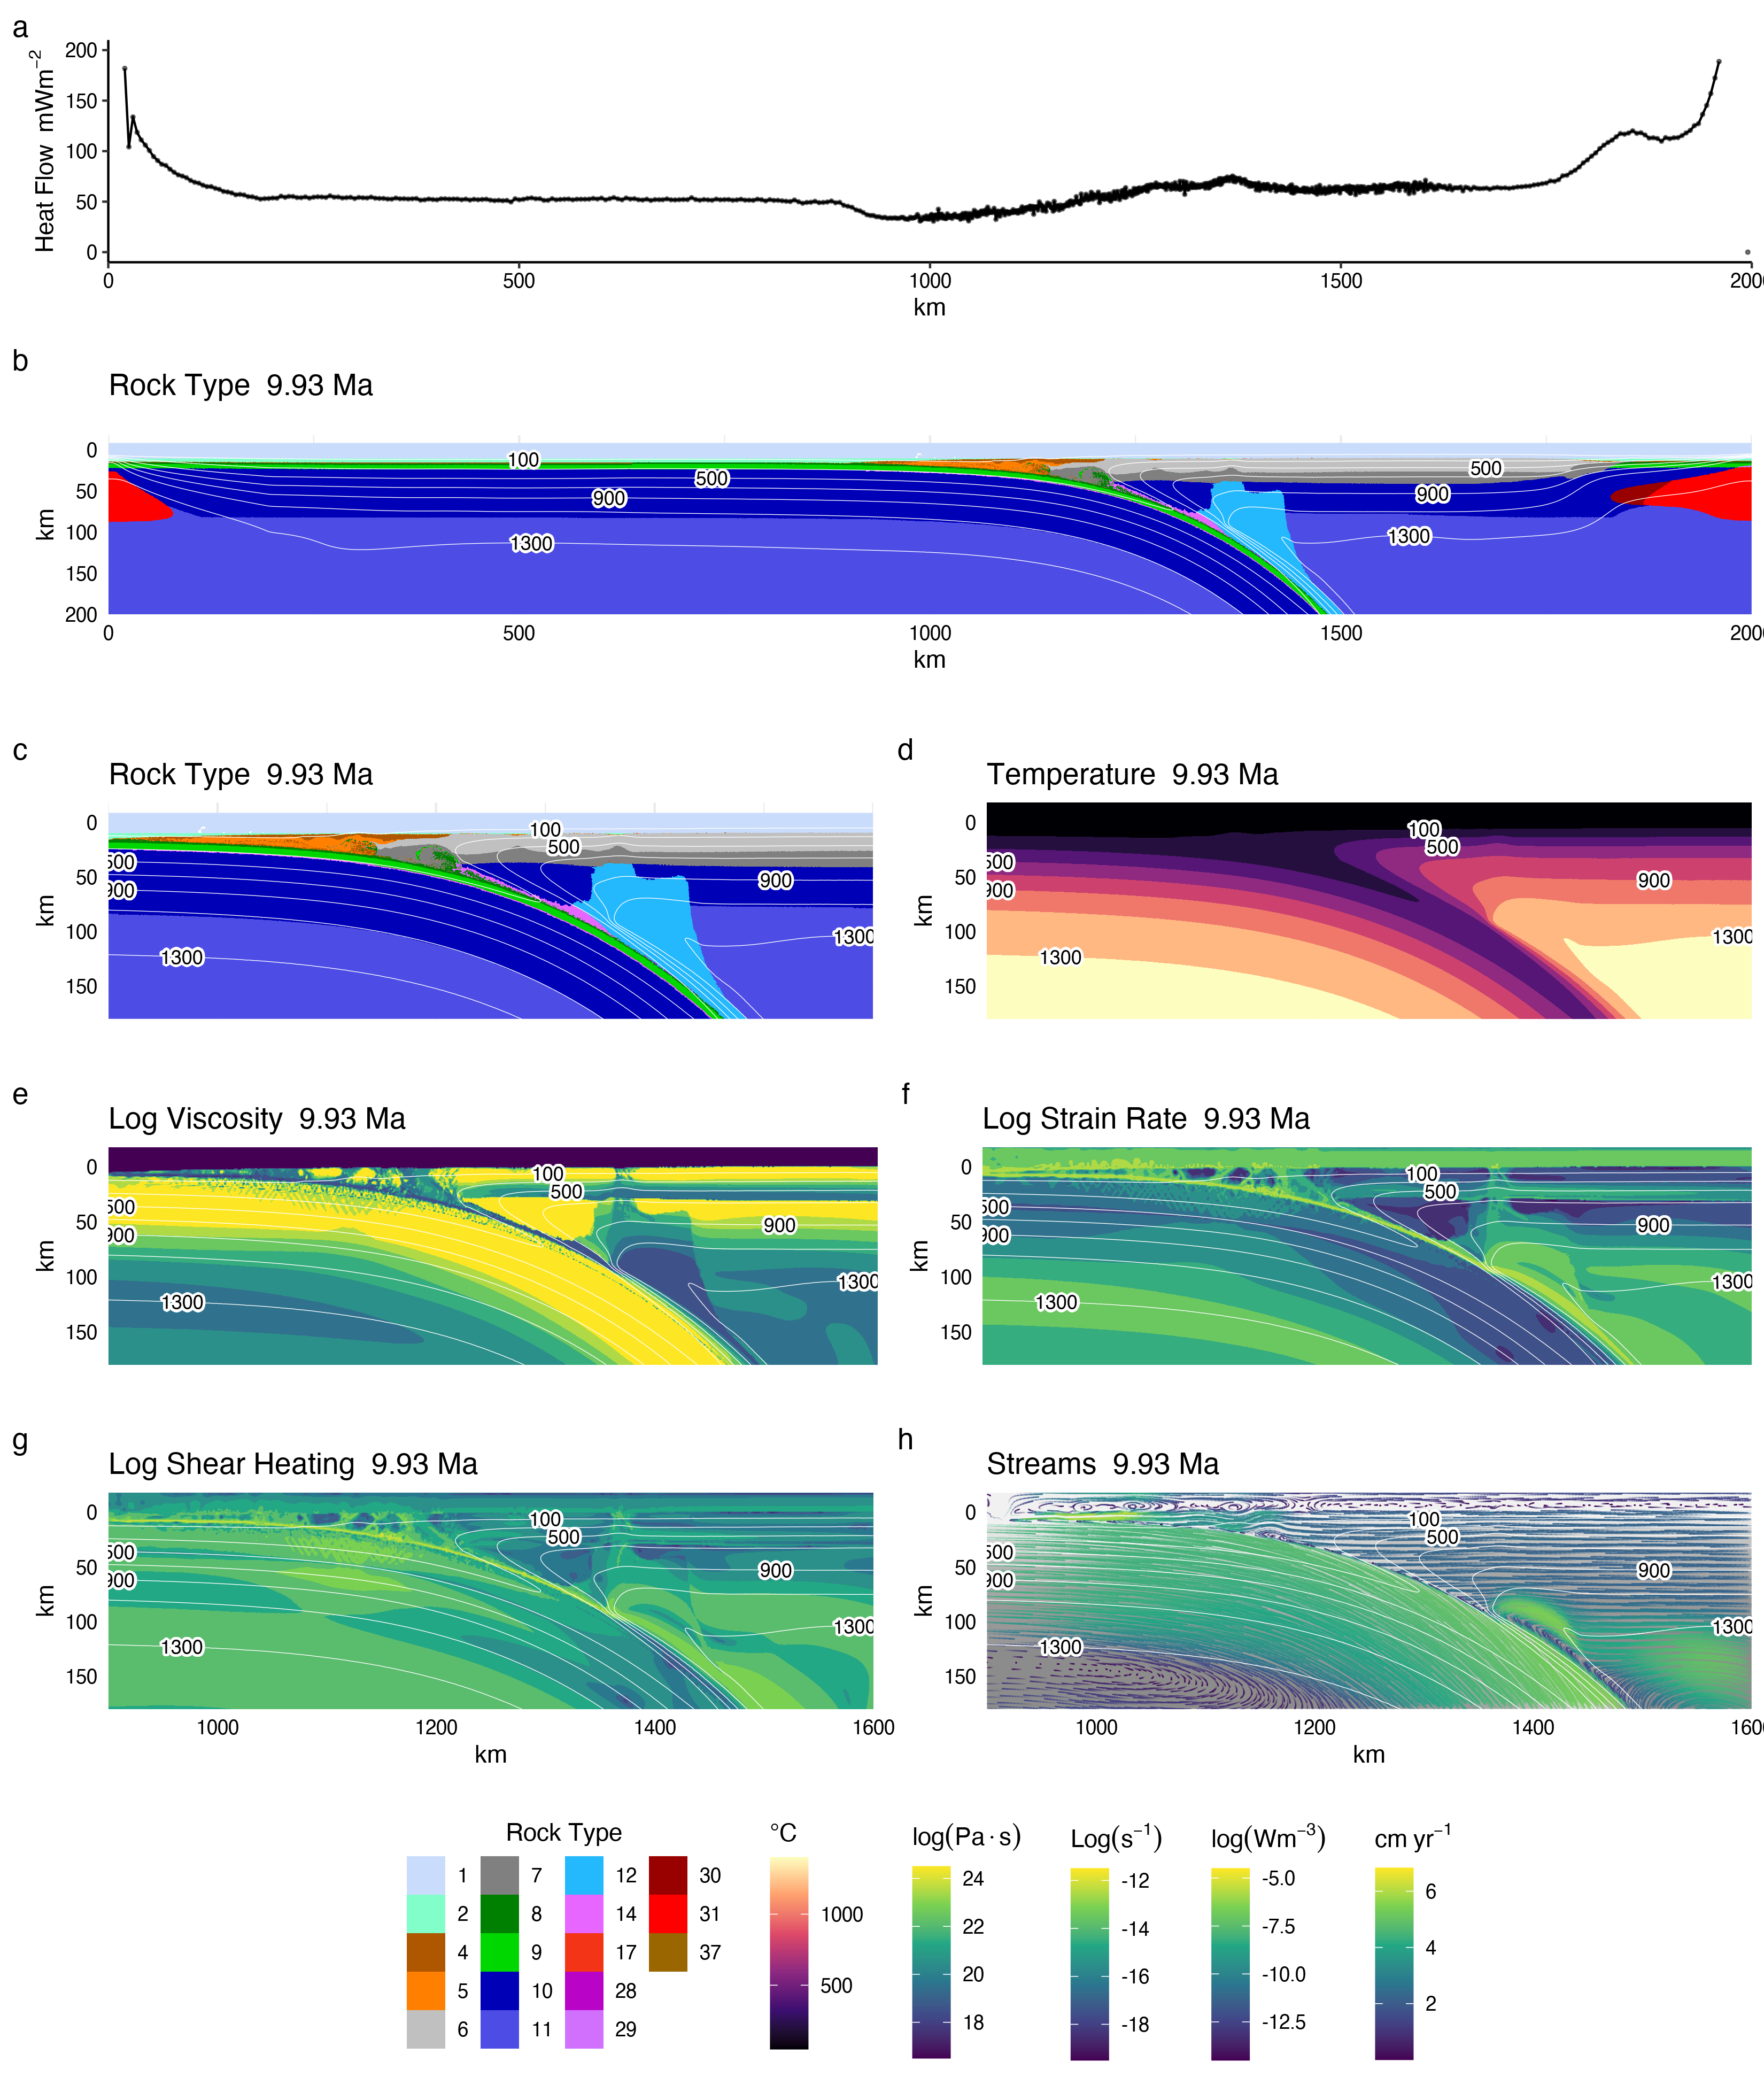
\includegraphics[width=1\linewidth,]{assets/figs/chpt2/fig3} 

}

\caption[Numerical experiment visualization]{Visualizing model cdf with a 78 $km$ upper-plate lithosphere at approximately 10 $Ma$. (a) Rock type shows a thin serpentine layer (pink) lubricating the plate interface. Note that low melt volumes are inconspicuous and quickly extracted. (b) Viscosity shows high contrast between the oceanic-plate and serpentinized upper-plate mantle at shallow levels. Viscosity contrast disappears where serpentine becomes unstable. (c) Streamlines show focused mantle flow towards the interface, coinciding with the lower limit of serpentine stability. Note the converging isotherms that imply a feedback between heat transfer, serpentine destabilization, and mechanical coupling. (d) Strain rate shows localized deformation in the serpentine layer along the plate interface. Note that deformation in the upper-plate mantle is restricted to viscous flow beneath the lithosphere and along narrow, subvertical melt conduits. Rock type colors are the same as Figure 1.}\label{fig:comp}
\end{figure}

After approximately 10 \(Ma\) of subduction coupling depth is determined directly from viscosity by finding the approximate area where strength contrasts between serpentinized- and non-serpentinized upper-plate mantle diminishes to \(<\) 10\(^2\) \(Pa \cdot s\). The node nearest to this region is assigned as the coupling depth. This study assumes mechanical coupling occurs instantaneously and at a single node. Mechanical coupling in reality must be dispersed across a finite length along the plate interface, however. At the numerical resolution the experiments, coupling-like viscosity contrasts are similar within a small area (approximately 5 \(\times\) 5 \(km\) or 5 \(\times\) 5 nodes), giving a qualitative uncertainty coupling depth on the order of 2.5 \(km\).

\hypertarget{chpt2Results}{%
\section{Results}\label{chpt2Results}}

\hypertarget{cdEstimators}{%
\subsection{Coupling Depth Estimators}\label{cdEstimators}}

Coupling depth (\(Z_{cpl}\)) correlates strongly with upper-plate thickness (\(Z_{UP}\)) and weakly with \(\Phi\) across all 64 numerical models (Table \ref{tab:zcResults}, Figures \ref{fig:results} \& \ref{fig:biv}). The responsiveness of coupling depth to \(Z_{UP}\) but not to \(\Phi\) is a key result of this study. The following equation minimizes standard least squares while optimizing the number of parameters, \emph{p value}, and \(R^2\) for all possible permutations of the variables \(Z_{UP}\) and \(\Phi\) in linear and quadratic forms:
\DIFdelbegin %DIFDELCMD < 

%DIFDELCMD < %%%
\DIFdelend \begin{equation}
  Z_{cpl} = 4.95\times 10^{-3}\ Z_{UP}^{2}\ -\ 9.27\times 10^{-2}\ \Phi\ +\ 63.6
  \label{eq:zCpl}
\end{equation}
\DIFdelbegin %DIFDELCMD < 

%DIFDELCMD < %%%
\DIFdelend where \(Z_{cpl}\) is coupling depth in \(km\) and \(\Phi\) is the thermal parameter in \(km/100\). Regression summaries show both linear and quadratic models of \(Z_{cpl}\) vs.~\(Z_{UP}\) and \(\Phi\) fit experimental results well (Tables \ref{tab:anova} \& \ref{tab:regSummary}). Equation \eqref{eq:zCpl} represents a statistical model formulated with observations from physics-based simulations of subduction. Equation \eqref{eq:zCpl} is useful for estimating coupling depths in active subduction zones where \(\Phi\) is known and \(Z_{UP}\) can be inverted from surface heat flow.

\begin{table}

\caption{\label{tab:segs}Estimated coupling depths for active subduction zones}
\centering
\begin{threeparttable}
\begin{tabular}[t]{lrrrrrr}
\toprule
Segment & $\vec{q}$ & $Z_{UP}$ & $\Phi$ & $Z_{cpl}^a$ & $Z_{cpl}^b$ & $Z_{cpl}^c$\\
\midrule
\cellcolor{gray!6}{N. Cascadia} & \cellcolor{gray!6}{75} & \cellcolor{gray!6}{74.2} & \cellcolor{gray!6}{3.4} & \cellcolor{gray!6}{92} & \cellcolor{gray!6}{91} & \cellcolor{gray!6}{90}\\
Nankai & 69 & 96.3 & 6.9 & 107 & 109 & 110\\
\cellcolor{gray!6}{Mexico} & \cellcolor{gray!6}{72} & \cellcolor{gray!6}{98.1} & \cellcolor{gray!6}{7.2} & \cellcolor{gray!6}{108} & \cellcolor{gray!6}{111} & \cellcolor{gray!6}{112}\\
Columbia-Ecuador & 80 & 66.4 & 10.4 & 86 & 84 & 84\\
\cellcolor{gray!6}{S.C. Chile} & \cellcolor{gray!6}{80} & \cellcolor{gray!6}{66.4} & \cellcolor{gray!6}{20.0} & \cellcolor{gray!6}{85} & \cellcolor{gray!6}{84} & \cellcolor{gray!6}{83}\\
\DIFdelbeginFL %DIFDELCMD < \addlinespace
%DIFDELCMD < %%%
\DIFdelendFL Kyushu & 69 & 83.2 & 13.5 & 97 & 97 & 96\\
\cellcolor{gray!6}{N. Sumatra} & \cellcolor{gray!6}{120} & \cellcolor{gray!6}{26.8} & \cellcolor{gray!6}{25.0} & \cellcolor{gray!6}{57} & \cellcolor{gray!6}{65} & \cellcolor{gray!6}{68}\\
Alaska & 80 & 66.4 & 25.3 & 85 & 83 & 82\\
\cellcolor{gray!6}{N. Chile} & \cellcolor{gray!6}{85} & \cellcolor{gray!6}{58.7} & \cellcolor{gray!6}{38.4} & \cellcolor{gray!6}{78} & \cellcolor{gray!6}{77} & \cellcolor{gray!6}{77}\\
N. Costa Rica & 80 & 58.5 & 20.4 & 80 & 79 & 78\\
\DIFdelbeginFL %DIFDELCMD < \addlinespace
%DIFDELCMD < %%%
\DIFdelendFL \cellcolor{gray!6}{Aleutians} & \cellcolor{gray!6}{75} & \cellcolor{gray!6}{51.6} & \cellcolor{gray!6}{39.6} & \cellcolor{gray!6}{73} & \cellcolor{gray!6}{73} & \cellcolor{gray!6}{73}\\
N. Hikurangi & 80 & 58.5 & 41.0 & 78 & 77 & 76\\
\cellcolor{gray!6}{Mariana} & \cellcolor{gray!6}{80} & \cellcolor{gray!6}{47.5} & \cellcolor{gray!6}{54.6} & \cellcolor{gray!6}{69} & \cellcolor{gray!6}{70} & \cellcolor{gray!6}{70}\\
Kermadec & 80 & 47.5 & 60.0 & 68 & 69 & 70\\
\cellcolor{gray!6}{Kamchatka} & \cellcolor{gray!6}{70} & \cellcolor{gray!6}{80.2} & \cellcolor{gray!6}{77.0} & \cellcolor{gray!6}{89} & \cellcolor{gray!6}{88} & \cellcolor{gray!6}{88}\\
\DIFdelbeginFL %DIFDELCMD < \addlinespace
%DIFDELCMD < %%%
\DIFdelendFL Izu & 80 & 47.5 & 77.0 & 67 & 68 & 68\\
\cellcolor{gray!6}{NE Japan} & \cellcolor{gray!6}{88} & \cellcolor{gray!6}{47.7} & \cellcolor{gray!6}{107.9} & \cellcolor{gray!6}{64} & \cellcolor{gray!6}{65} & \cellcolor{gray!6}{65}\\
\bottomrule
\end{tabular}
\begin{tablenotes}
\item \uline{\textit{key}}: $\vec{q}$: average backarc surface heat flow $[mWm^{-2}]$, $Z_{UP}$: upper-pate thickness $[km]$, $\Phi$: thermal parameter = $[km/100]$, $Z_{cpl}$: coupling depth $[km]$
\item \uline{\textit{estimators}}: a: $[Z_{cpl}=Z_{UP}+\Phi]$, b: $[Z_{cpl}=Z_{UP}^2+\Phi]$, c: $[Z_{cpl}=Z_{UP}+Z_{UP}^2+\Phi]$
\item \uline{\textit{references}}: Currie \& Hyndman (2006), Wada \& Wang (2009)
\end{tablenotes}
\end{threeparttable}
\end{table}

Sensitivity of coupling depth to upper-plate thickness and \(\Phi\) is apparent when visualizing Equation \eqref{eq:zCpl} and other regression models across \(Z_{UP}\) and \(\Phi\) space \ref{fig:multiv}. Applying Equation \eqref{eq:zCpl} to 17 active subduction zone segments (Table \ref{tab:segs}) gives a wide range of estimated coupling depths, similar to the numerical simulations in this study. The distribution of estimated coupling depths, however, is relatively narrow and quasi-normal, with a mean of \(\sim\) 82 \(km\) and standard deviation of 7 \(km\) (Figure \ref{fig:multiv}d).

\begin{figure}[htbp]

{\centering 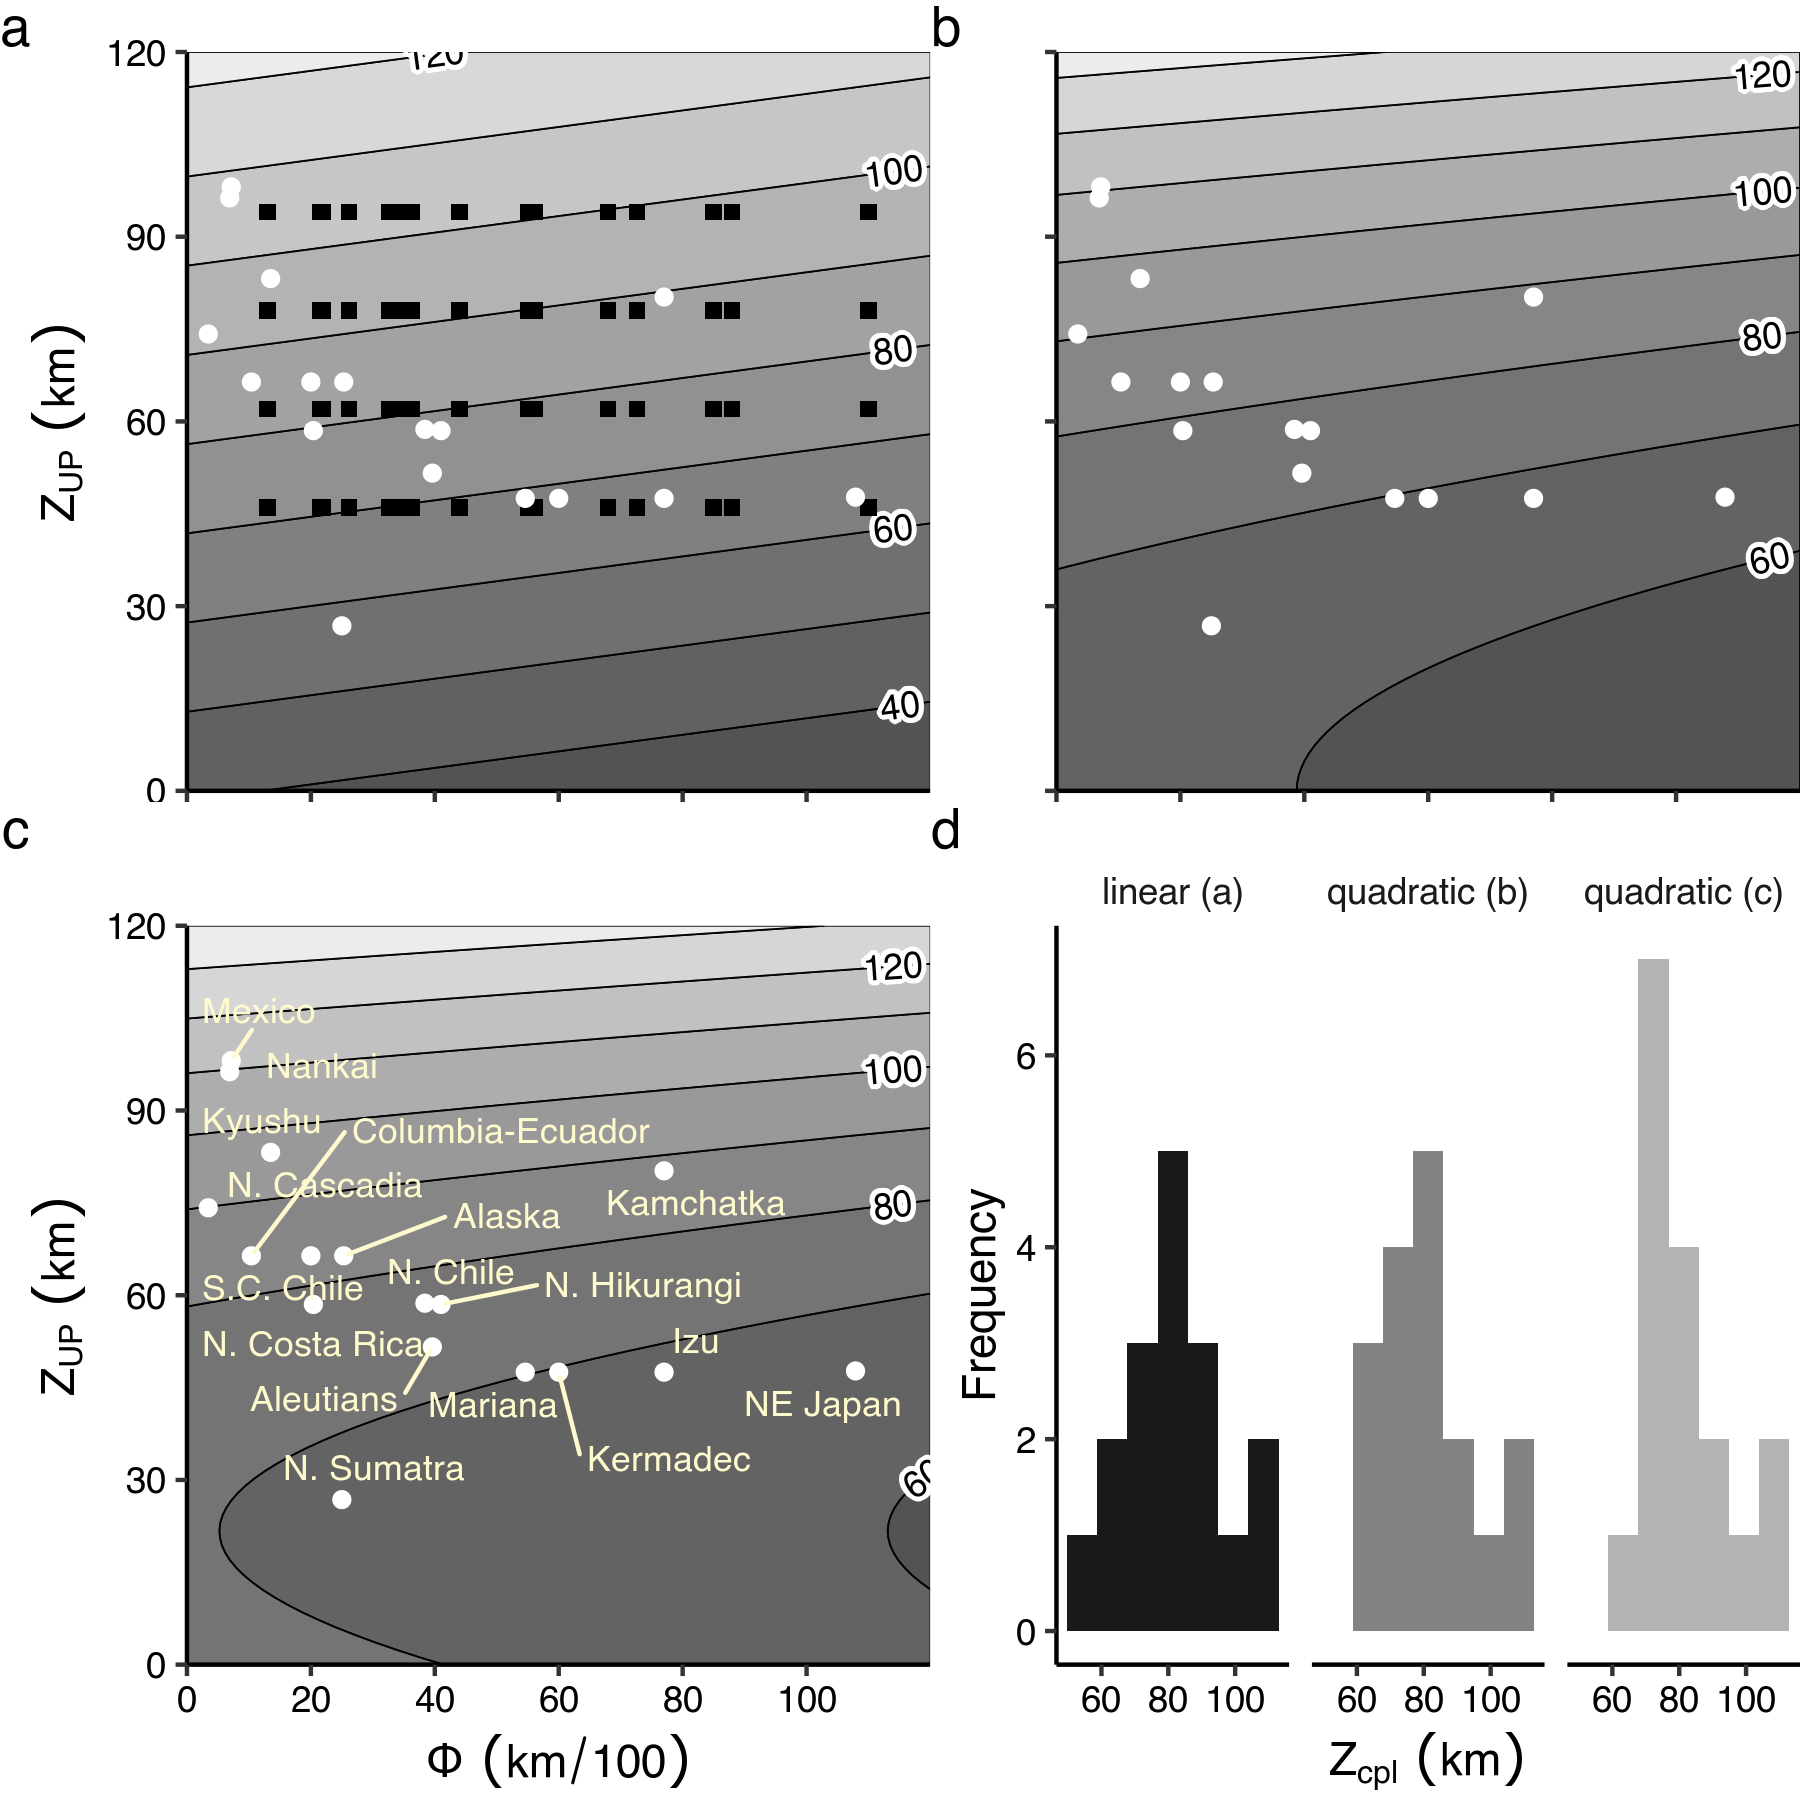
\includegraphics[width=1\linewidth,]{assets/figs/chpt2/fig4} 

}

\caption[Estimated coupling depths for 17 active subduction zone segments]{Multivariate regressions and estimated coupling depth ($Z_{cpl}$) for 17 active subduction zone segments. Contoured plots show estimated $Z_{cpl}$ (contours) as a function of thermal parameter ($\Phi$) and upper-plate thickness ($Z_{UP}$) for linear (a) and quadratic (b, c) regressions. The best fit regression is panel b (Equation \ref{eq:zCpl}, see Tables \ref{tab:anova} and \ref{tab:regSummary}). Black squares \DIFdelbeginFL \DIFdelFL{represent }\DIFdelendFL \DIFaddbeginFL \DIFaddFL{are }\DIFaddendFL numerical experiments used to fit the contours. White points represent active subduction zones (Table \ref{tab:segs}). Contours imply $Z_{cpl}$ depends strongly on $Z_{UP}$\DIFdelbeginFL \DIFdelFL{, regardless of the regression equation form}\DIFdelendFL . \DIFdelbeginFL \DIFdelFL{Estimated }\DIFdelendFL \DIFaddbeginFL \DIFaddFL{While some estimated }\DIFaddendFL $Z_{cpl}$ for subduction zones with similar $\Phi$ are quite different (e.g. Alaska vs. N. Sumatra)\DIFdelbeginFL \DIFdelFL{. Estimated }\DIFdelendFL \DIFaddbeginFL \DIFaddFL{, some estimated }\DIFaddendFL $Z_{cpl}$ are \DIFdelbeginFL \DIFdelFL{also }\DIFdelendFL quite similar for subduction zones with very different $\Phi$ (e.g. Kamchatka vs. N. Cascadia). (d) Distributions of estimated $Z_{cpl}$ for 17 active subduction zones shown in (a), (b), and (c). These 17 segments span a large range of $\Phi$ but are expected to have a relatively narrow distribution of $Z_{cpl}$ (82 $\pm$ 14 $km$) according to the regressions in (a), (b), and (c).}\label{fig:multiv}
\end{figure}

\hypertarget{surface-heat-flow}{%
\subsection{Surface Heat Flow}\label{surface-heat-flow}}

Upper-plate surface heat flow remains relatively stable and reflects initial upper-plate geotherms in the backarc region for experiments with low to moderate \(\Phi\) (Figure \ref{fig:hf}). However, high-amplitude and high-frequency positive surface heat flow deviations in the upper-plate are common in all experiments, especially for high-\(\Phi\) experiments. These deviations correspond to extensional deformation and heat transport via lithospheric thinning and melt migration. These features are apparent as subvertical low viscosity, high strain rate columns originating from the plate interface (Figure \ref{fig:comp}b, d) and point to potential sources of error when inverting surface heat flow in active subduction zones. Notably, the backarc is relatively unaffected by fluid and melt migration compared to the forearc. Estimating upper-plate thickness by inverting surface heat flow in the backarc is therefore preferable to forearc surface heat flow.

Surface heat flow across all numerical experiments is similar in the forearc region (normalized distance \(\leq\) 0.75, Figure \ref{fig:hf78}). In contrast, surface heat flow extending behind the arc region (normalized distance \(>\) 0.75, Figure \ref{fig:hf78}) increases systematically, then levels off at values reflecting initial continental geotherms (i.e.~reflecting initial upper-plate thickness). In reality, surface heat flow depend on fault slip rates and rates of volcanic outputs. However, heat flow in the behind the arc may remain in steady-state if rates of volcanism and crustal thinning by extension are low (\protect\hyperlink{ref-currie2004}{Currie et al., 2004}; \protect\hyperlink{ref-currie2006}{Currie \& Hyndman, 2006}).

\begin{figure}[htbp]

{\centering 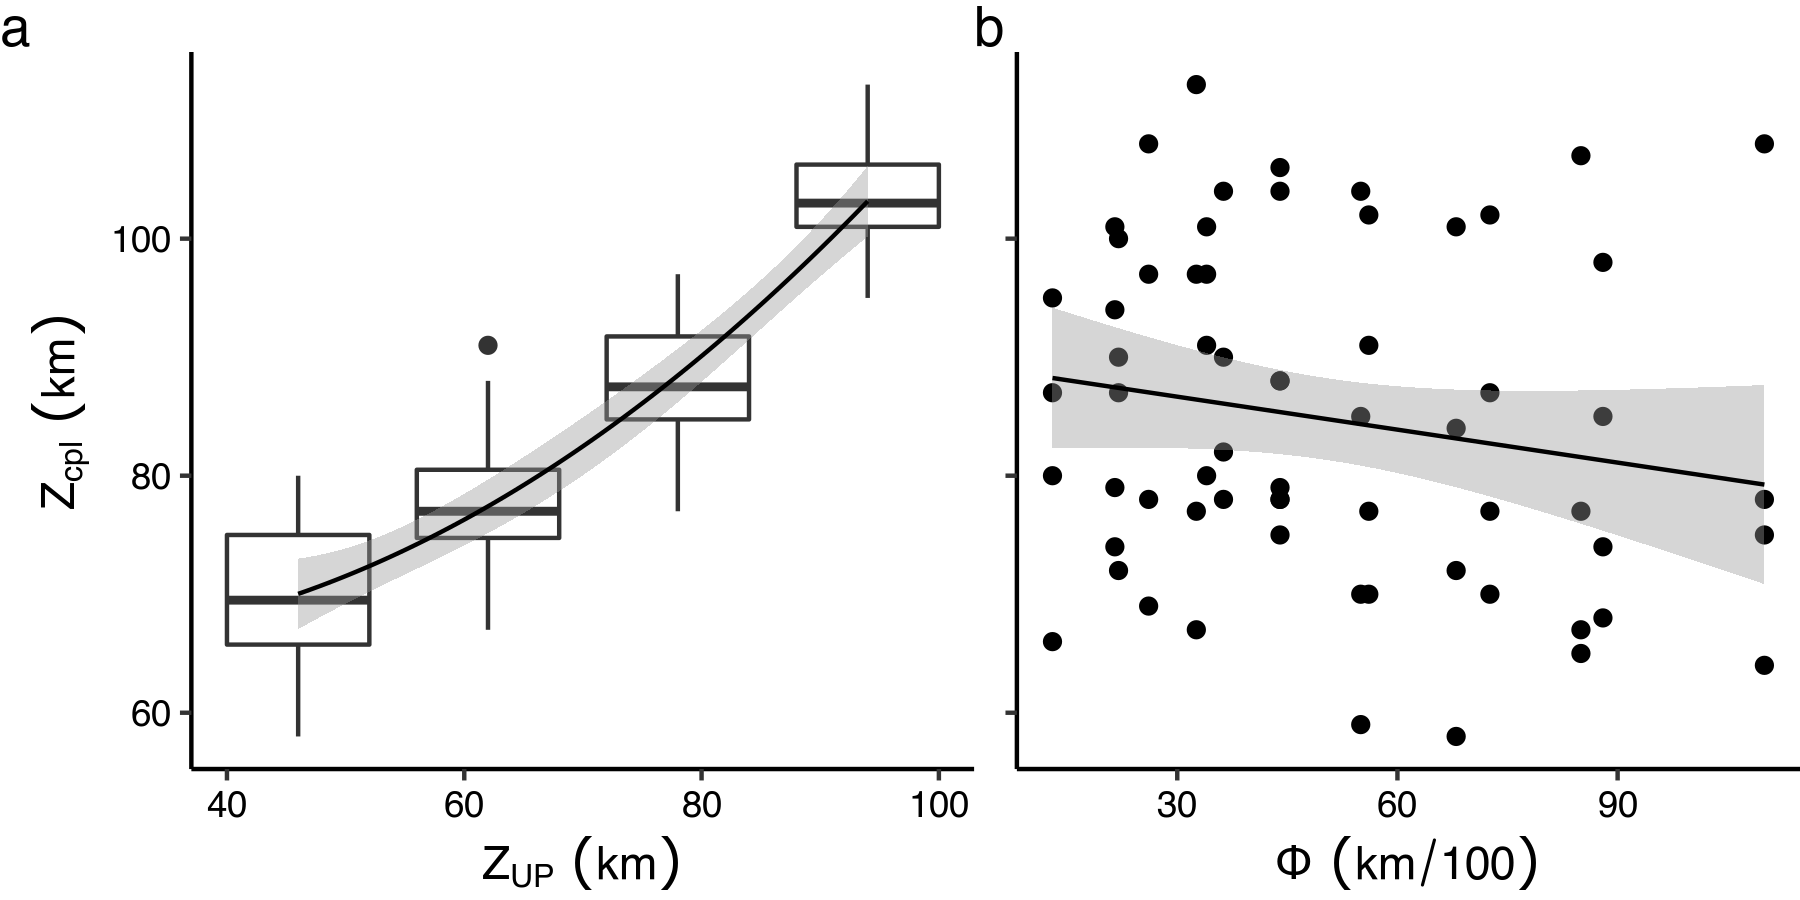
\includegraphics[width=1\linewidth,]{assets/figs/chpt2/fig5} 

}

\caption[Surface heat flow calculated from numerical experiments]{Surface heat flow ($\vec{q}$) vs. normalized distance for model cdf with upper-plate thickness ($Z_{UP}$) ranging from 46 to 94 $km$. The distribution of $\vec{q}$ in the forearc (normalized distance between 0.0 and 1.0) is narrow and shows little variance until near the arc (normalized distance between 0.75 and 1.0). The broad distribution of $\vec{q}$ behind the arc (normalized distance $>$ 1.0) reflects the broad distribution of initial continental geotherms ($Z_{UP}$). Any simple relationship between $\vec{q}$ and $Z_{UP}$ may be obscured by heating from extension or vertical migration of fluids, especially within the arc-region (high-amplitude fluctuations).}\label{fig:hf78}
\end{figure}

\hypertarget{chpt2Discussion}{%
\section{Discussion}\label{chpt2Discussion}}

\hypertarget{dynamic-feedbacks-regulating-plate-coupling}{%
\subsection{Dynamic Feedbacks Regulating Plate Coupling}\label{dynamic-feedbacks-regulating-plate-coupling}}

A clear association between plate coupling and the reaction \(antigorite \allowbreak \Leftrightarrow olivine + orthopyroxene + H_{2}O\) is observed in all experiments. A relatively narrow serpentine channel quickly forms above the dehydrating oceanic-plate, localizing strain, lubricating the plate interface, and inhibiting transfer of shear stress between plates (e.g., \protect\hyperlink{ref-agard2016}{Agard et al., 2016}; \protect\hyperlink{ref-ruh2015}{Ruh et al., 2015}). This mechanical behavior is a direct consequence of a sharp rheologic change dependent on the location of serpentine dehydration reaction described in Section \ref{numHydration} and its effect on the rheologic model described in Section \ref{rheologicModel}. Interactions among viscosity changes, serpentine dehydration, and heat transfer are regulated by competing dynamic feedbacks acting in the upper-plate. In summary, cooling and hydration of the shallow upper-plate mantle (serpentine stabilization) and heating from circulating asthenospheric mantle beneath the upper-plate lithosphere (driven by mechanical coupling) compete to stabilize coupling depth (Figure \ref{fig:flow}).

The entire process can be conceptualized with Figure \ref{fig:flow} as follows. The upper-plate mantle cools via diffusive heat loss to the oceanic-plate along the entire length of the plate interface (Figure \ref{fig:flow}a). At shallow depths, water released from the oceanic-plate stabilizes serpentine in the overriding upper-plate mantle, effectively decoupling the two plates (Figure \ref{fig:flow}b, point a). A positive feedback stabilizes serpentine to greater depths as decoupled plates stagnate the upper-plate mantle, promoting further cooling and formation of serpentine. Numerical experiments imply only a thin layer of serpentine is sufficient to trigger this feedback.

\DIFaddbegin \begin{figure}[htbp]

{\centering 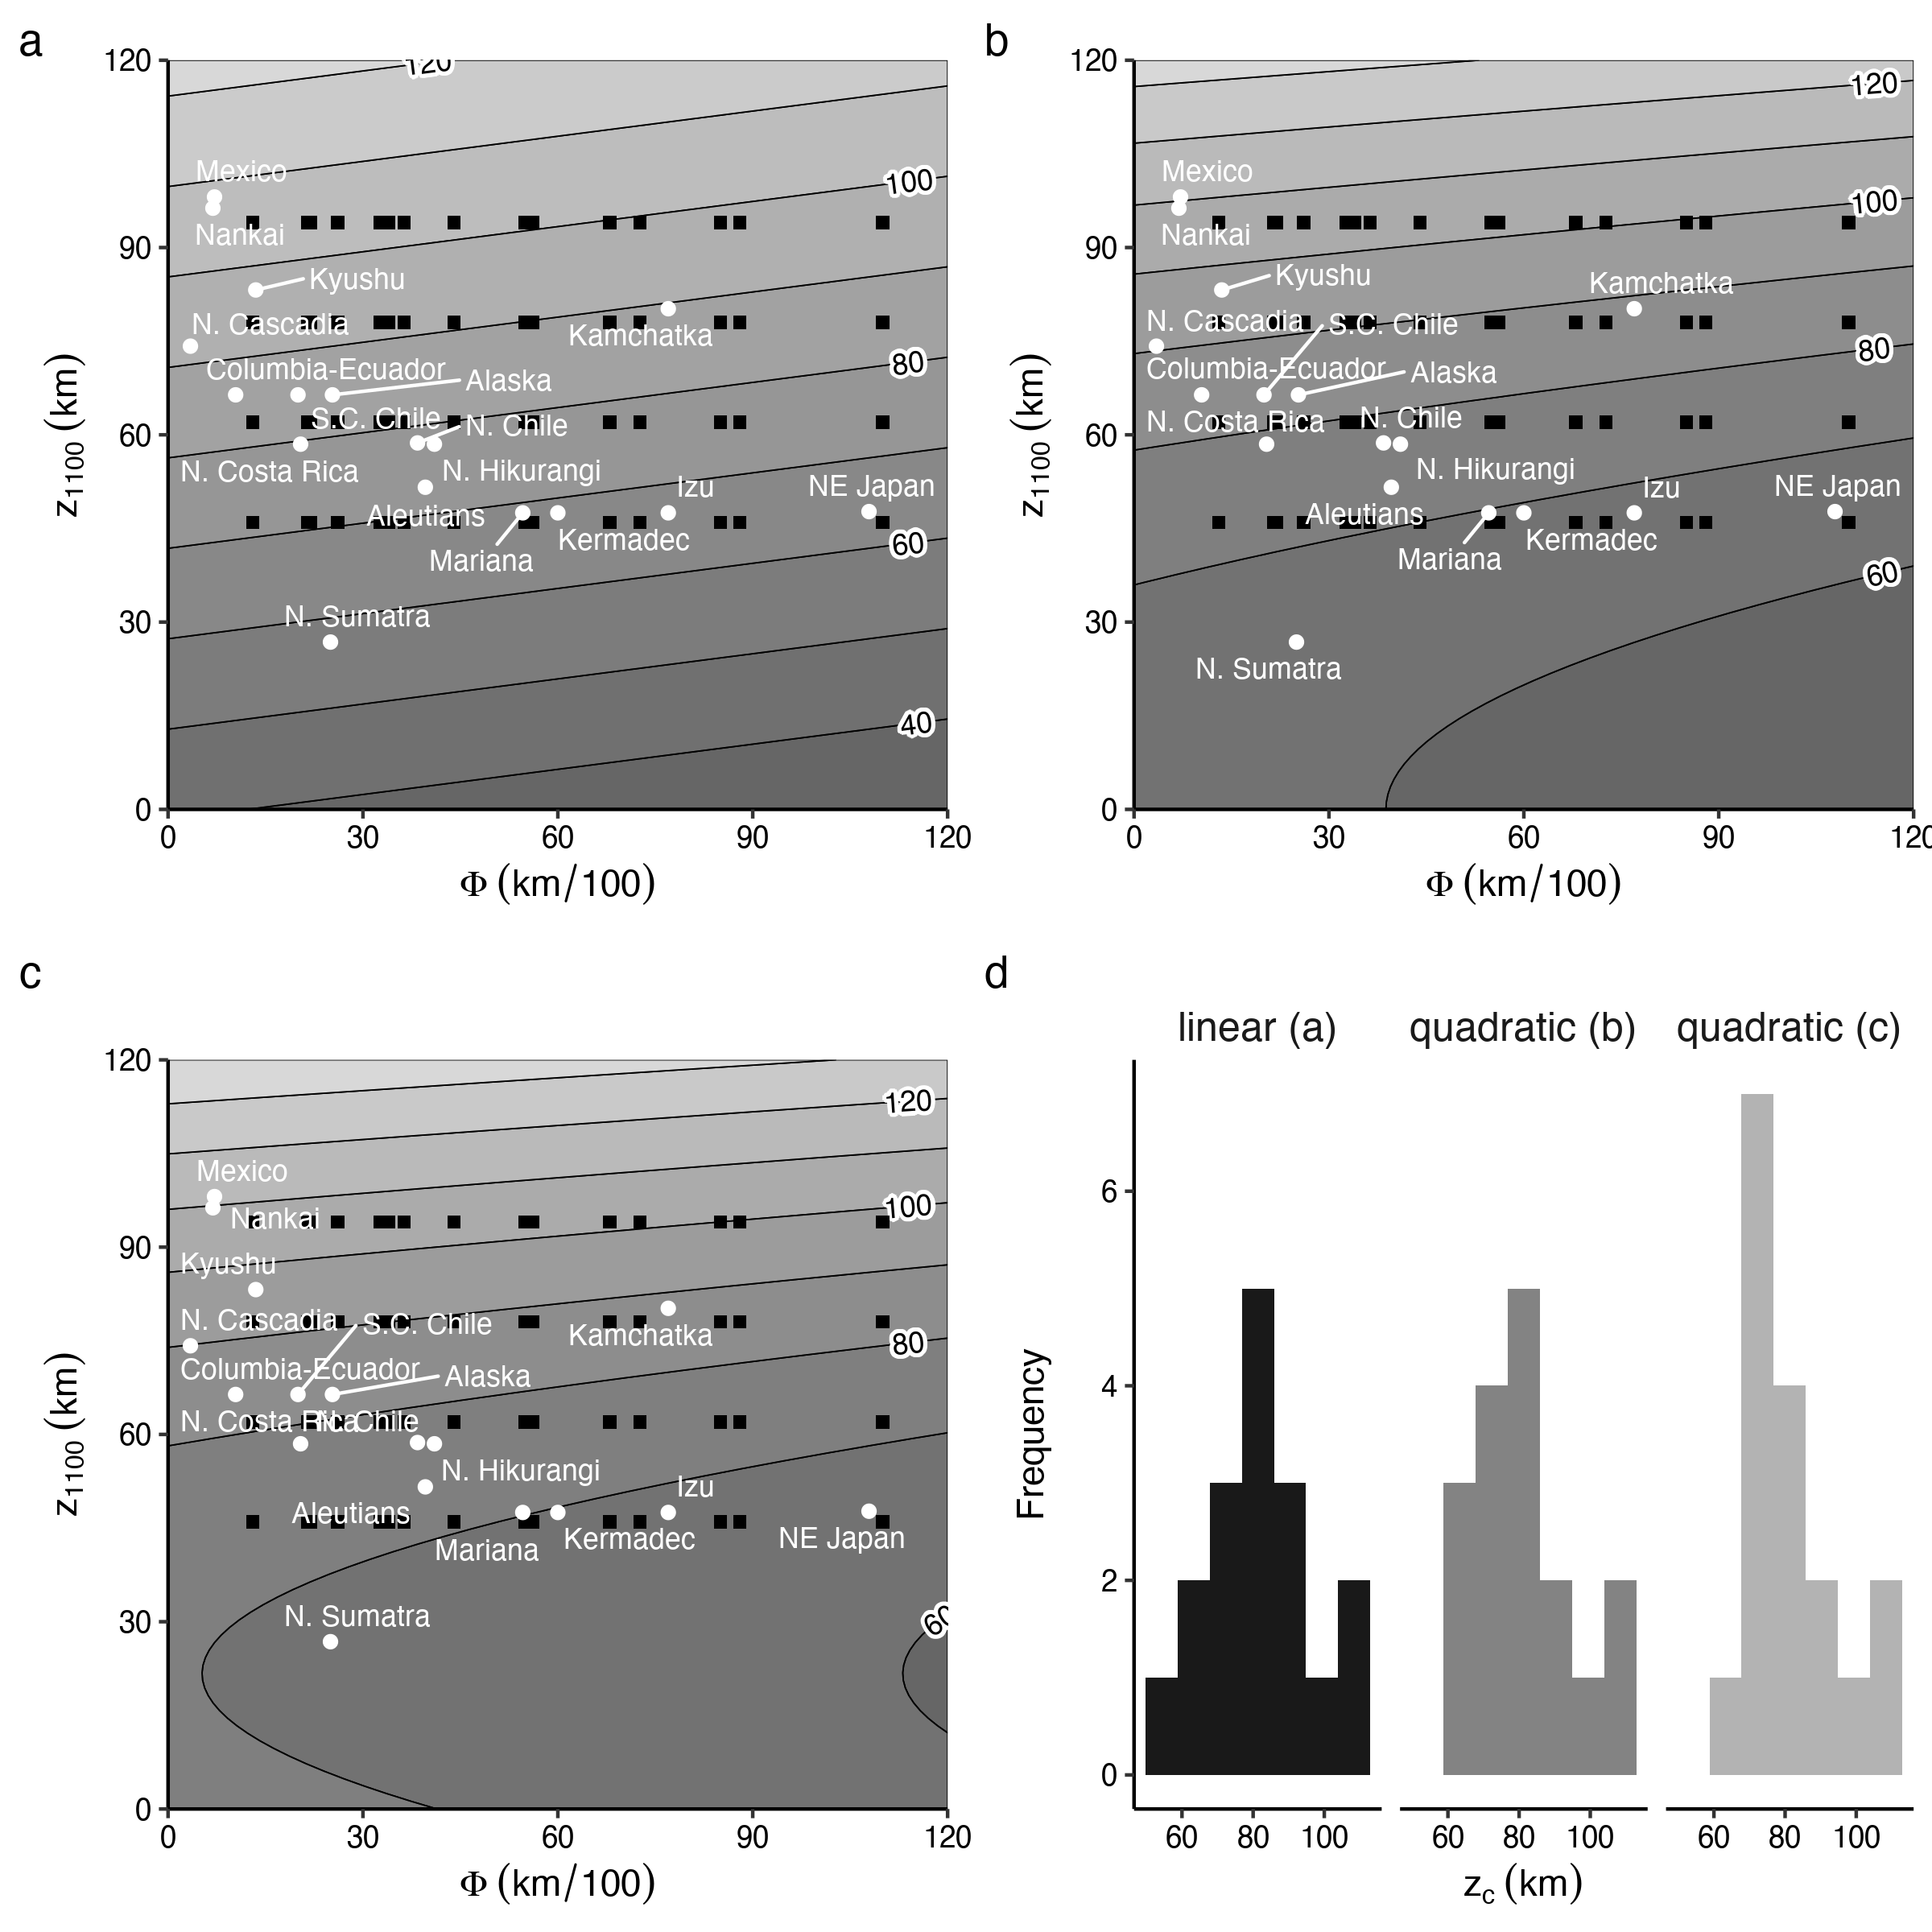
\includegraphics[width=1\linewidth,]{assets/figs/chpt2/fig6} 

}

\caption[Visualizing viscosity and mantle flow]{\DIFaddFL{Visualizing viscosity and mantle flow near the coupling region at approximately 10 $Ma$ for model cdf with upper-plate thickness of 78 $km$. Strong mantle flow beneath the lithospheric base (1100$^{\circ}C$) transfers heat towards the coupling region. Viscosity indicates coupling at the point where the viscosity contrast between the slab and mantle approaches zero (between points b \& d). Reference points a-e are used for discussing coupling dynamics and thermal feedbacks (see Section \ref{cplResponses}).}}\label{fig:flow}
\end{figure}

\DIFaddend Deeper along the plate interface, beyond the stability of serpentine, diffusive heat loss from the upper-plate mantle to the slab forms a thickening layer of high-viscosity mantle atop the oceanic-plate (Figure \ref{fig:flow}b, point b). Downward motion of the oceanic-plate, plus accreted high-viscosity mantle (Figure \ref{fig:flow}b, point b) relative to the deepest extent of the stiff upper-plate mantle (Figure \ref{fig:flow}b, point c) creates a pressure gradient that attracts flow of the weakest materials---serpentine from the up-dip direction (Figure \ref{fig:flow}b, point d)---and hot mantle from below (Figure \ref{fig:flow}b, point e). Flow of hot mantle into the necking region between points b and c in Figure \ref{fig:flow} is analogous to passive asthenospheric upwelling toward a mid-ocean ridge where two strong cooling lithospheric plates diverge. Highly efficient heat advection from the warm upper-plate asthenospheric mantle (Figure \ref{fig:flow}a) prevents formation of sperentine---thus regulating and stabilizing the coupling depth.

Coupling mechanics apparent from numerical experiments can be described in terms of competing positive and negative feedbacks. The positive feedback involves addition of water into a diffusively cooling, shallow mantle to produce serpentine. The negative feedback involves serpentine destabilization by advection of heat from the deeper upper-plate asthenospheric mantle. Such thermal-petrologic-mechanical feedbacks drive coupling depth towards steady-state. The numerical experiments in this study imply a finely-tuned balance of serpentine stability can maintain coupling depths in subduction zones for potentially 10's of Ma.

\hypertarget{cplResponses}{%
\subsection{\texorpdfstring{Coupling Responses to \(Z_{UP}\) and \(\Phi\)}{Coupling Responses to Z\_\{UP\} and \textbackslash Phi}}\label{cplResponses}}

How does upper-plate thickness influence coupling depth? Numerical experiments point to the upper-plate lithosphere-asthenosphere boundary as an important feature constraining coupling mechanics as it defines the permissible flow field in the upper-plate (Figure \ref{fig:streams}a-d). Thin upper-plate lithospheres (Figure \ref{fig:streams}a, b) permit shallow mantle flow and advection of heat farther up the plate interface. Thin upper-plate lithospheres thereby raise coupling depths by raising serpentine stability up the plate interface. Thick upper-plate lithospheres (Figure \ref{fig:streams}c, d) restrict mantle wedge flow to deeper levels, deepening serpentine stability and mechanical coupling.

The thermal state of the slab, as represented by \(\Phi\), has almost no effect on coupling depth by comparison. Relative insensitivity of coupling depth to \(\Phi\) is consistent with previous studies of active subduction zones (\protect\hyperlink{ref-furukawa1993}{Furukawa, 1993}; \protect\hyperlink{ref-wada2009}{Wada \& Wang, 2009}). The irresponsiveness of coupling depth to changes in \(\Phi\) is perhaps due to competing cooling and heating effects driven by the subducting oceanic-plate. For example, high-\(\Phi\) oceanic-plates (older plates with higher velocities) cool the upper-plate mantle more effectively, but also effectively heat the interface by driving stronger mantle circulation. In contrast, low-\(\Phi\) oceanic-plates (younger plates with lower velocities) are less effective in cooling the upper-plate mantle, but also ineffectively heat the interface by ineffectively driving mantle circulation. That is, the shallow vs.~deep dynamic effects of \(\Phi\) tend to cancel each other, explaining the lack of correlation between coupling depth and \(\Phi\).

\DIFdelbegin %DIFDELCMD < \begin{figure}[htbp]
%DIFDELCMD < 

%DIFDELCMD < {\centering 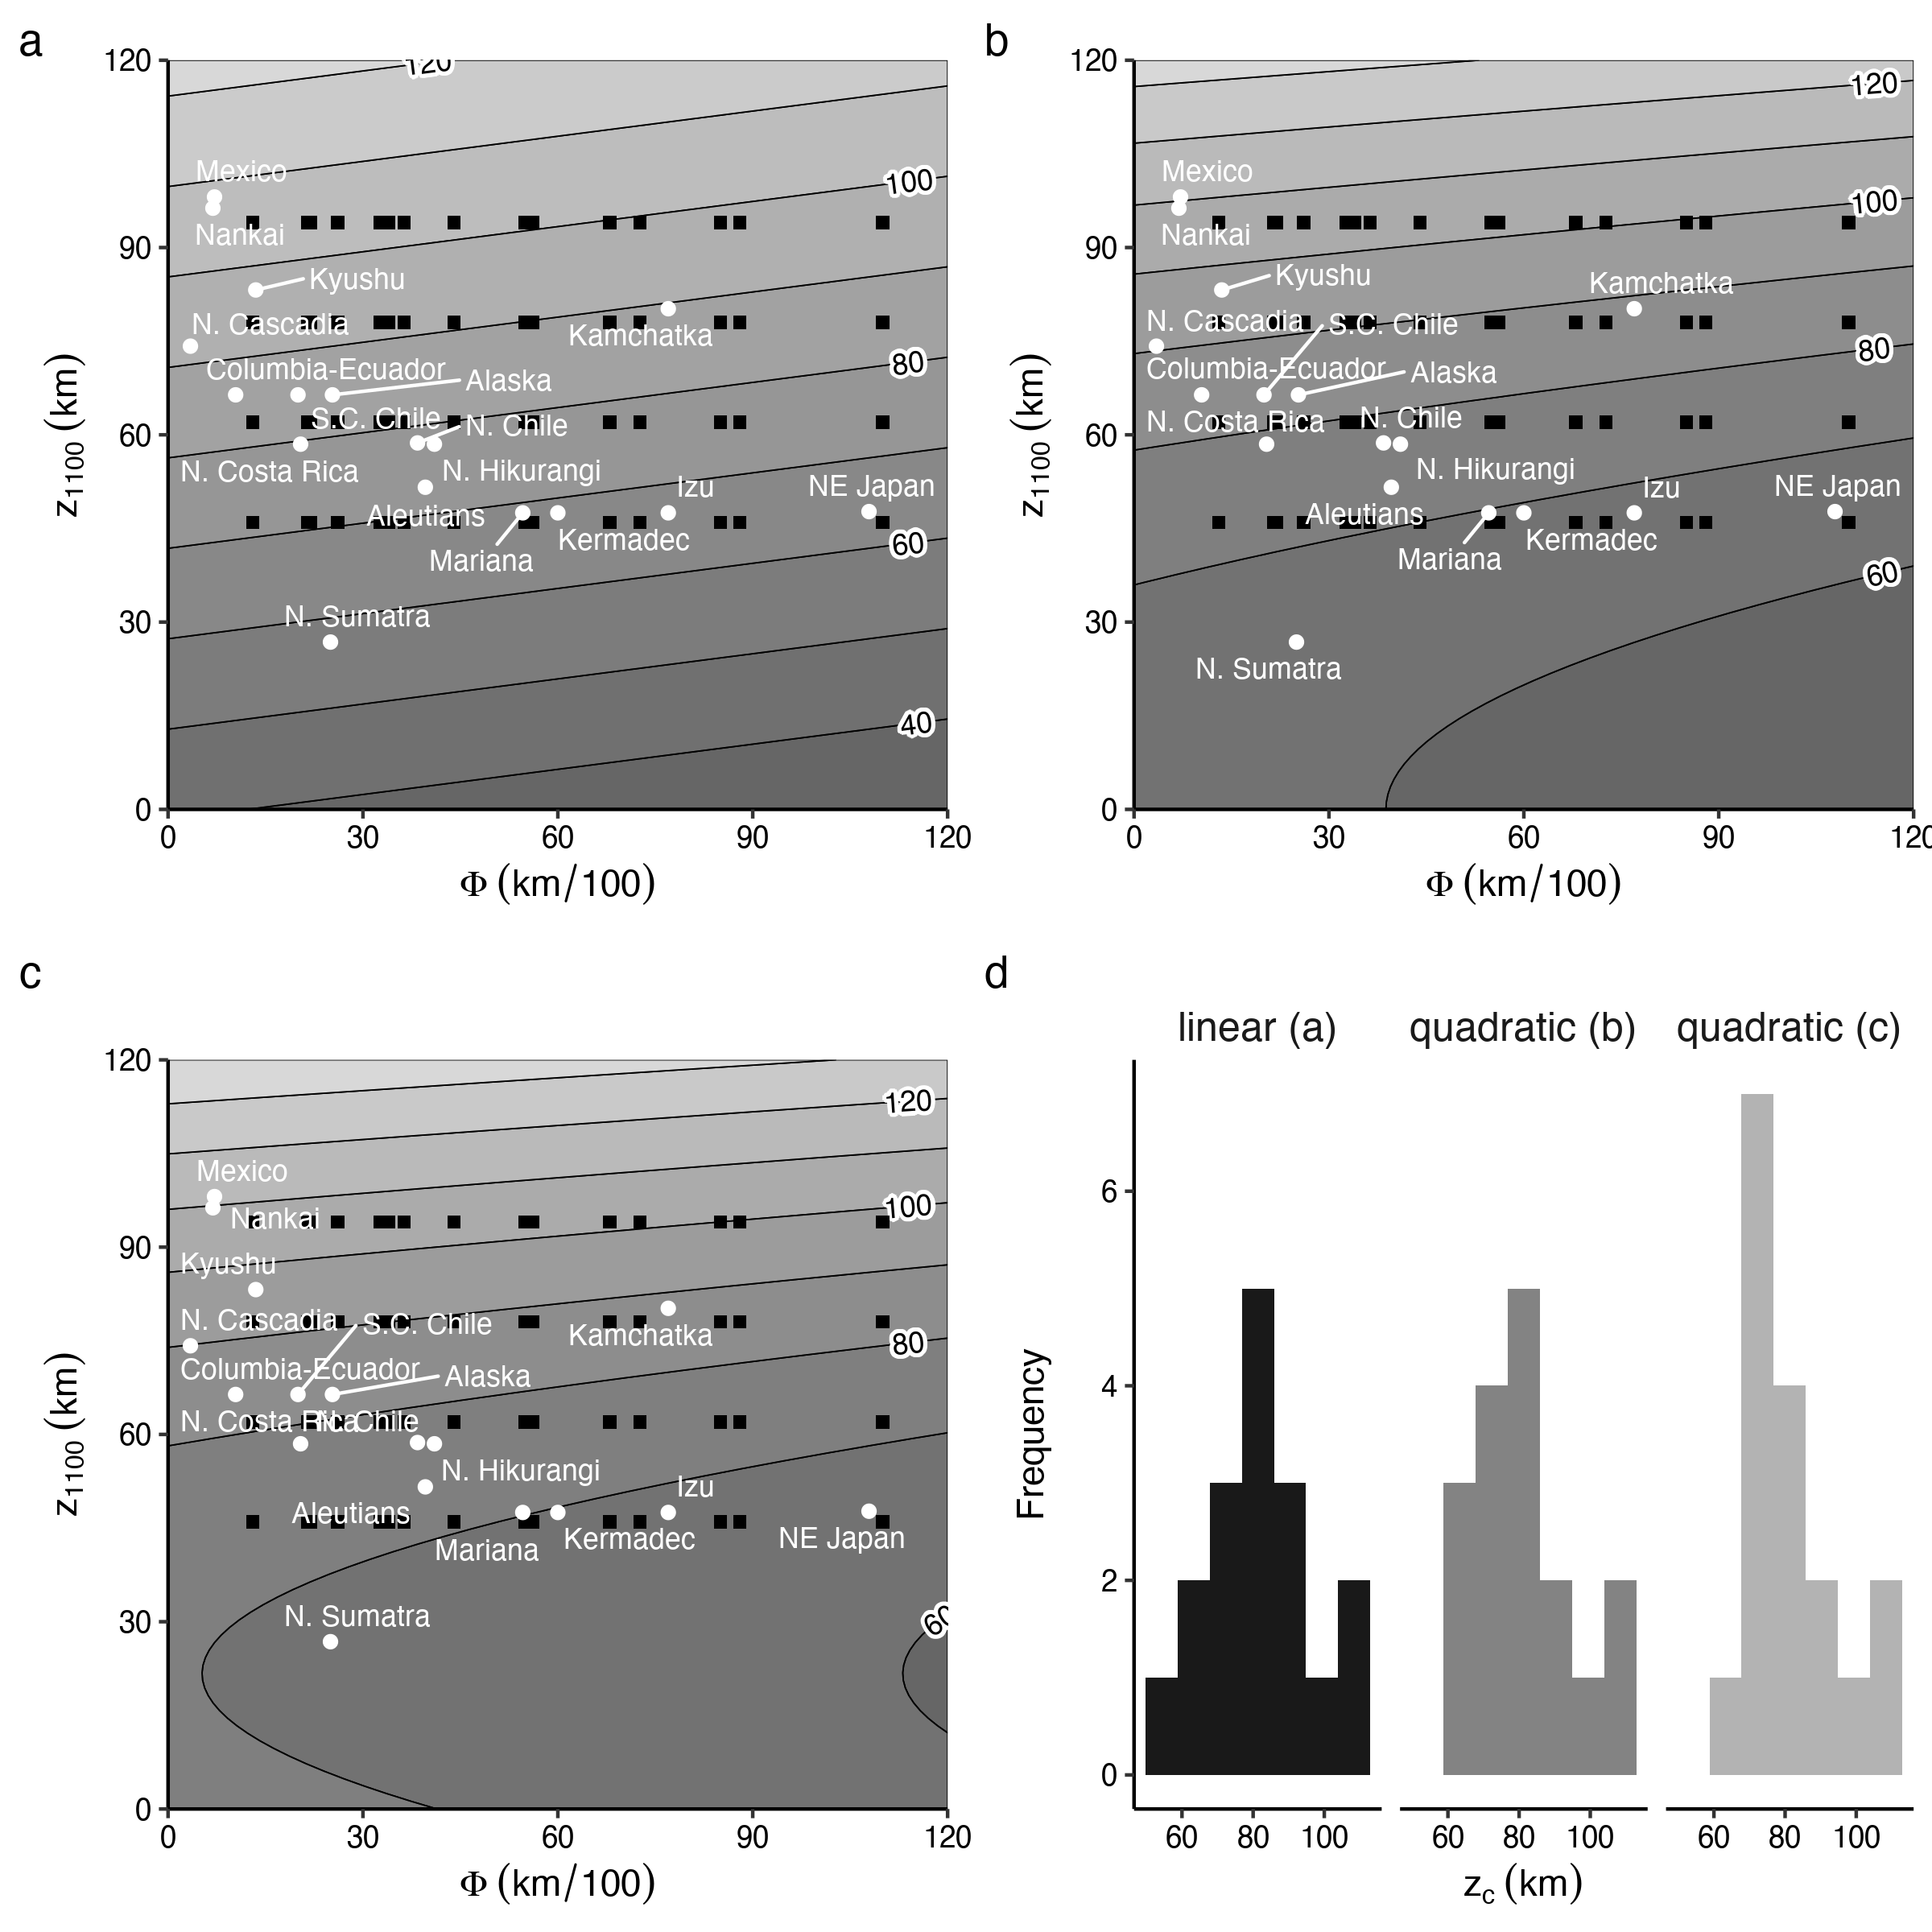
\includegraphics[width=1\linewidth,]{assets/figs/chpt2/fig6} 
%DIFDELCMD < 

%DIFDELCMD < }
%DIFDELCMD < 

%DIFDELCMD < %%%
%DIFDELCMD < \caption[Visualizing viscosity and mantle flow]{%
{%DIFAUXCMD
\DIFdelFL{Visualizing viscosity and mantle flow near the coupling region at approximately 10 $Ma$ for model cdf with upper-plate thickness of 78 $km$. Strong mantle flow beneath the lithospheric base (1100$^{\circ}C$) transfers heat towards the coupling region. Viscosity indicates coupling at the point where the viscosity contrast between the slab and mantle approaches zero (between points b \& d). Reference points a-e are used for discussing coupling dynamics and thermal feedbacks (see Section \ref{cplResponses}).}}%DIFAUXCMD
%DIFDELCMD < \label{fig:flow}
%DIFDELCMD < \end{figure}
%DIFDELCMD < 

%DIFDELCMD < %%%
\DIFdelend \hypertarget{estimating-coupling-depths-in-subduction-zones}{%
\subsection{Estimating Coupling Depths in Subduction Zones}\label{estimating-coupling-depths-in-subduction-zones}}

Theoretically, coupling depth can be estimated directly by fitting forearc surface heat flow data using forward modelling approaches (e.g., \protect\hyperlink{ref-wada2009}{Wada \& Wang, 2009}). However, forward approaches typically adjust coupling depth independently from upper-plate thickness, which is inconsistent with an inherent link between coupling depth and upper-plate thickness discussed in Section \ref{chpt2Discussion} (e.g.~Figures \ref{fig:hf78} \& \ref{fig:streams}). Moreover, many additional heat sources (e.g.~shear heating and crustal plutonism, \protect\hyperlink{ref-gao2014}{Gao \& Wang, 2014}; \protect\hyperlink{ref-reesjones2018}{Rees Jones et al., 2018}) may contribute to forearc surface heat flow---increasing uncertainty when inverting upper-plate thickness from surface heat flow.

Assuming low degrees of backarc extension, estimating coupling depth in active subduction zones using Equation \eqref{eq:zCpl} with \(Z_{UP}\) inverted from backarc surface heat flow is preferable to avoid additional uncertainties stemming from seismic and volcanic activity in the forearc. However, while \(\Phi\) is inventoried for most active subduction zones (\protect\hyperlink{ref-syracuse2006}{Syracuse \& Abers, 2006}), a corresponding dataset of \(Z_{UP}\) does not exist. Several geophysical and petrologic methods might be considered for independent estimates of \(Z_{UP}\) (e.g.~seismic velocities, flexure, heat flow, mantle xenoliths). Backarc surface heat flow is still a good choice, however, because of its direct correspondence with \(Z_{UP}\). For example, \(Z_{UP}\) may be estimated using simple one-dimensional heat transport models assuming values for radiogenic heat production in the crust (\protect\hyperlink{ref-rudnick1998}{Rudnick et al., 1998}). Special attention must be paid to crustal processes, including extension and magmatism, because additional heating will underestimate \(Z_{UP}\) and, consequently, underestimate coupling depth.

\begin{figure}[htbp]

{\centering 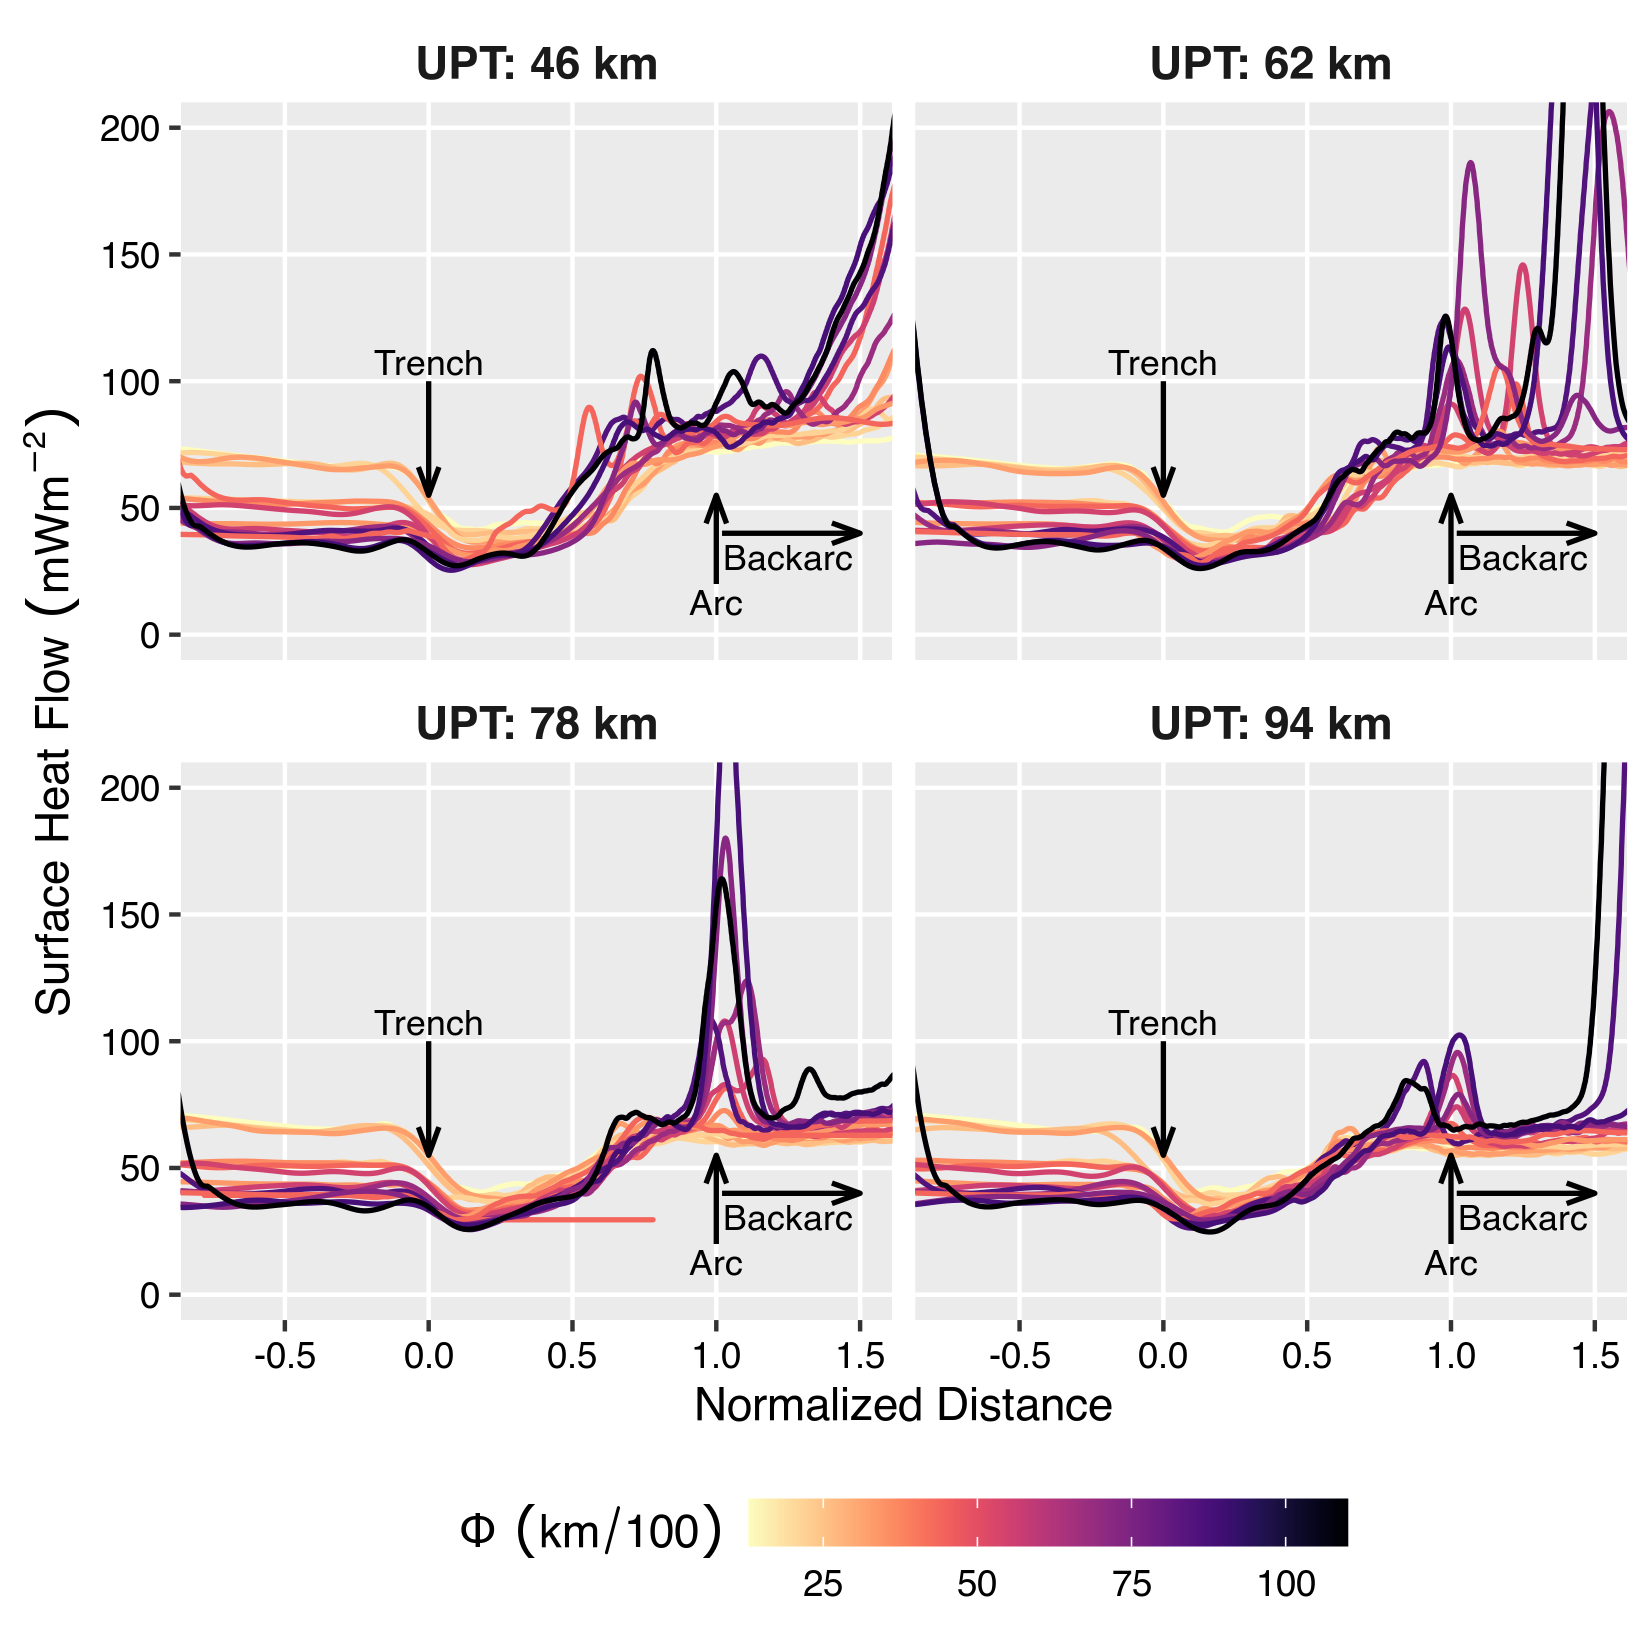
\includegraphics[width=1\linewidth,]{assets/figs/chpt2/fig7} 

}

\caption[Visualizing mantle flow and coupling by upper-plate thickness]{Visualizing mantle flow at approximately 10 $Ma$ for model cdf with upper-plate thickness of (a) 46, (b) 62, (c) 78, and (d) 94 $km$. All experiments are plotted on the same scale and location within the model domain. The flow of warm mantle is restricted to below the 1100$^{\circ}C$ isotherm, which corresponds to the base of the upper-plate lithosphere ($Z_{UP}$). A minimum coupling depth ($Z_{cpl}$) appears to exist as models with extremely thin lithospheres (a) exhibit coupling at $\sim$ 70-80 $km$ depth. $Z_{cpl}$ generally increases with increasing $Z_{UP}$ as mantle flow and advective heat transport are restricted to greater depths.}\label{fig:streams}
\end{figure}

\hypertarget{globally-similar-coupling-depths}{%
\subsection{Globally Similar Coupling Depths?}\label{globally-similar-coupling-depths}}

A \(Z_{cpl}\) distribution of 82 \(\pm\) 14 \(km\) (2\(\sigma\)) estimated for active subduction zones in this study (Figure \ref{fig:multiv}d) roughly match the preferred \(Z_{cpl}\) inferred from forearc surface heat flow for Cascadia and NE Japan (75-80 \(km\), \protect\hyperlink{ref-syracuse2010}{Syracuse et al., 2010}; \protect\hyperlink{ref-wada2009}{Wada \& Wang, 2009}) \(km\). The range of \(Z_{cpl}\) estimated for active subduction zones in this study (Figure \ref{fig:multiv}d) is relatively broad, however. For example, omitting Mexico and Nankai because their \(\Phi\) values fall outside the range of \(\Phi\) used for numerical experiments, estimated coupling depths range from almost 100 \(km\) (Kyushu) to approximately 65 \(km\) (Sumatra and NE Japan, Table \ref{tab:segs}).

Coupling depth in active subduction zones are commonly assumed to be narrowly distributed around 70-80 \(km\) (\protect\hyperlink{ref-syracuse2010}{Syracuse et al., 2010}; \protect\hyperlink{ref-wada2009}{Wada \& Wang, 2009}). The strong correlation between \(Z_{UP}\) and \(Z_{cpl}\) found from numerical experiments imply uniform coupling depths are possible if upper-plate thickness are globally uniform. The surface heat flow dataset compiled by Wada \& Wang (\protect\hyperlink{ref-wada2009}{2009}) (Table \ref{tab:segs}) shows average backarc surface heat flow are indeed similar among active subduction zones---implying a narrow distribution of coupling depths (Figure \ref{fig:multiv}d). Much of their dataset is based on Currie \& Hyndman (\protect\hyperlink{ref-currie2006}{2006}), who estimate upper-plate thickness for 10 circum-Pacific subduction zones of 50-60 \(km\) (defined by the 1200 \(^{\circ}C\) isotherm). Uniformly thin upper-plate thickness are corroborated by uniformly high heat flow (\(>\) 70 \(mW/m^{2}\)), thermobarometric constraints on mantle xenoliths, and P-wave velocities (\protect\hyperlink{ref-currie2006}{Currie \& Hyndman, 2006}). An attempt is made to further corroborate the uniformity of upper-plate thickness in Chapter \ref{chpt3} by interpolating surface heat flow near active subduction zones.

Although it still curious why upper-plates among subduction zones may have similar thicknesses, one can assume it is likely related to some processes of lithospheric erosion proposed for subarc lithosphere. These include: lithospheric delamination induced by lower crust eclogitization (\protect\hyperlink{ref-sobolev2005}{Sobolev \& Babeyko, 2005}), small-scale convection caused by hydration-induced mantle wedge weakening (\protect\hyperlink{ref-arcay2006}{Arcay et al., 2006}), thermal erosion (\protect\hyperlink{ref-england2010}{England \& Katz, 2010}), mechanical weakening by percolating melts (\protect\hyperlink{ref-gerya2011}{Gerya \& Meilick, 2011}), and subarc foundering of magmatic cumulates (\protect\hyperlink{ref-jull2001}{Jull \& Kelemen, 2001}). Most of these mechanisms are thus strongly related to mantle wedge hydration, melting, and melt transport toward volcanic arcs.

The metamorphic rock record may also imply consistency among coupling depths in subduction zones. For example, the demise of a serpentine channel and onset of coupling may provide a natural barrier such that rocks are more likely to be exhumed from within the channel than from below it. The relative abundance of blueschists and eclogites should then be greater for pressures below estimated coupling depths (approximately 2.4 \(GPa\) or 70-80 \(km\)) than above them. This hypothesis will be explicitly explored in Chapter \ref{chpt4}.

\hypertarget{conclusions}{%
\section{Conclusions}\label{conclusions}}

Three important results are highlighted in this study:

\begin{enumerate}
\def\labelenumi{\arabic{enumi}.}
\item
  Coupling depth is stabilized near the base of the upper-plate lithosphere by competing dynamic feedbacks regulating heat transport, serpentine dehydration, and mechanical coupling in the upper-plate mantle.
\item
  A simple expression fitted to coupling depths observed in numerical experiments allows the coupling depths to be estimated for active subduction zones by inverting upper-plate thickness from surface heat flow.
\item
  Uniform surface heat flow in circum-Pacific subduction zones (\protect\hyperlink{ref-currie2006}{Currie \& Hyndman, 2006}; \protect\hyperlink{ref-wada2009}{Wada \& Wang, 2009}) may indicate uniform coupling depths at approximately 80 \(km\).
\end{enumerate}

Questions remain, however, including: how do warm (thin) upper-plates persist over 100's of kilometers behind arcs and throughout the lifespan of subduction zones? How abruptly are dehydration reaction occurring along the subduction interface? How can expressions like Equation \eqref{eq:zCpl} be improved using natural datasets? Each of these questions may be considered for future research.

\cleardoublepage

\hypertarget{chpt3}{%
\chapter{A Comparison of Heat Flow Interpolations Near Subduction Zones}\label{chpt3}}

\markboth{Chapter 3: Heat Flow Interpolations}{Chapter 3: Heat Flow Interpolations}

\DIFdelbegin %DIFDELCMD < \begin{quote}
%DIFDELCMD < %%%
\textbf{\DIFdel{Keypoints:}}
%DIFAUXCMD
%DIFDELCMD < 

%DIFDELCMD < \begin{itemize}
\begin{itemize}%DIFAUXCMD
%DIFDELCMD < \item
\item%DIFAUXCMD
%DIFDELCMD <   %%%
\DIFdel{Spatial patterns of surface heat flow near subduction zones reflect regional geodynamic variability
}%DIFDELCMD < \item
\item%DIFAUXCMD
%DIFDELCMD <   %%%
\DIFdel{Fundamentally different interpolation methods, Kriging and Similarity, both show cases of along-strike variability in average upper-plate surface heat flow
}%DIFDELCMD < \item
\item%DIFAUXCMD
%DIFDELCMD <   %%%
\DIFdel{Variations in upper-plate surface heat flow imply non-uniform upper-plate thickness and discontinuous geodynamics
}
\end{itemize}%DIFAUXCMD
%DIFDELCMD < \end{itemize}
%DIFDELCMD < \end{quote}
%DIFDELCMD < 

%DIFDELCMD < %%%
\DIFdelend \hypertarget{chpt3Abstract}{%
\section{Abstract}\label{chpt3Abstract}}

The magnitude of heat fluxing through the Earth's surface is directly proportional to the magnitude of temperature gradients and strain rates within Earth's crust and upper mantle. Global heat flow databases are thus promising sources for generating and testing hypotheses about subduction geodynamics. However, evaluating surface heat flow across large tectonic features requires careful projection and interpolation of sparse observations. This study compares two interpolation methods based on fundamentally different principles, Kriging and Similarity, to investigate spatial variability of surface heat flow near 13 presently active subduction zones. Kriging and Similarity are grossly comparable at regional scales with median differences from -2 to 14 \(mWm^{-2}\). More importantly, Kriging and Similarity both show distinctive trench-perpendicular surface heat flow patterns along strike within the upper-plates of 7 out of 13 segments. Moreover, average upper-plate surface heat flow can differ up to 50 \(mWm^{-2}\) along a single subduction zone segment. Subduction zone segments with discontinuous upper-plate surface heat flow may reflect spatially heterogeneous lithospheric thickness (contrary to expectations from Chapter \ref{chpt2}), spatially heterogeneous dynamics, spatially heterogeneous near-surface perturbations, and/or undersampling relative to the scale and magnitude of spatial variability. Subduction zone segments with continuous upper-plate surface heat flow may imply the opposite. Potential explanations for a nearly 50\%-50\% split between segments with (dis)continuous upper-plate surface heat flow patterns is yet to be identified and warrants further investigation.

\hypertarget{chpt3Intro}{%
\section{Introduction}\label{chpt3Intro}}

Surface heat flow databases (\protect\hyperlink{ref-hasterok2008}{Hasterok \& Chapman, 2008}; \protect\hyperlink{ref-jennings2021}{Jennings \& Hasterok, 2021}; \protect\hyperlink{ref-lucazeau2019}{Lucazeau, 2019}; \protect\hyperlink{ref-pollack1993}{Pollack et al., 1993}) enable geodynamic investigations by relating the amount of heat escaping Earth's surface to heat-transferring and heat-generating subsurface processes like hydrothermal circulation, radioactive decay, fault motion, and mantle convection (\protect\hyperlink{ref-currie2004}{Currie et al., 2004}; \protect\hyperlink{ref-currie2006}{Currie \& Hyndman, 2006}; \protect\hyperlink{ref-fourier1827}{Fourier, 1827}; \protect\hyperlink{ref-furlong2013}{Furlong \& Chapman, 2013}; \protect\hyperlink{ref-furukawa1993}{Furukawa, 1993}; \protect\hyperlink{ref-gao2014}{Gao \& Wang, 2014}; \protect\hyperlink{ref-hasterok2013}{Hasterok, 2013}; \protect\hyperlink{ref-kelvin1863}{Kelvin, 1863}; \protect\hyperlink{ref-kerswell2020}{Kerswell et al., 2020}; \protect\hyperlink{ref-parsons1977}{Parsons \& Sclater, 1977}; \protect\hyperlink{ref-pollack1977}{Pollack \& Chapman, 1977}; \protect\hyperlink{ref-rudnick1998}{Rudnick et al., 1998}; \protect\hyperlink{ref-stein1992}{Stein \& Stein, 1992}, \protect\hyperlink{ref-stein1994}{1994}; \protect\hyperlink{ref-wada2009}{Wada \& Wang, 2009}). Surface heat flow observations have motivated research in many scientific and industrial fields as evident by more than 1,393 publications compiled in the largest and most recent surface heat flow database (ThermoGlobe, \protect\hyperlink{ref-jennings2021}{Jennings \& Hasterok, 2021}; \protect\hyperlink{ref-lucazeau2019}{Lucazeau, 2019}).

While ThermoGlobe currently contains 69,729 observations, the regional coverage near subduction zones is uneven and irregularly-spaced (\DIFdelbegin \DIFdel{Table \ref{tab:hfSummaryTable} \& Figure \ref{fig:globalhfComp} }\DIFdelend \DIFaddbegin \DIFadd{Figure \ref{fig:globalhfComp} \& Table \ref{tab:hfSummaryTable}}\DIFaddend ). Many methods may be considered to interpolate surface heat flow including inverse distance weighting, various splines and linear regressions, nearest-neighbor, general additive models, Kriging, and Similarity, to name a few. Generally speaking, these methods predict surface heat flow across a grid of arbitrarily defined locations with unknown surface heat flow (the targets) by fitting mathematical models to available surface heat flow observations (the examples). The two interpolation methods compared in this study, Kriging and Similarity, are chosen because they represent end-member methodological classes based on fundamentally different principles. Their comparative differences, therefore, may be important for advancing understanding of subduction zone processes, for targeting areas for future heat flow research, for improving either method in the context of subduction zone research, and for developing new layered interpolation methods that combine the strengths of Kriging and Similarity techniques.

\begin{figure}[htbp]

{\centering 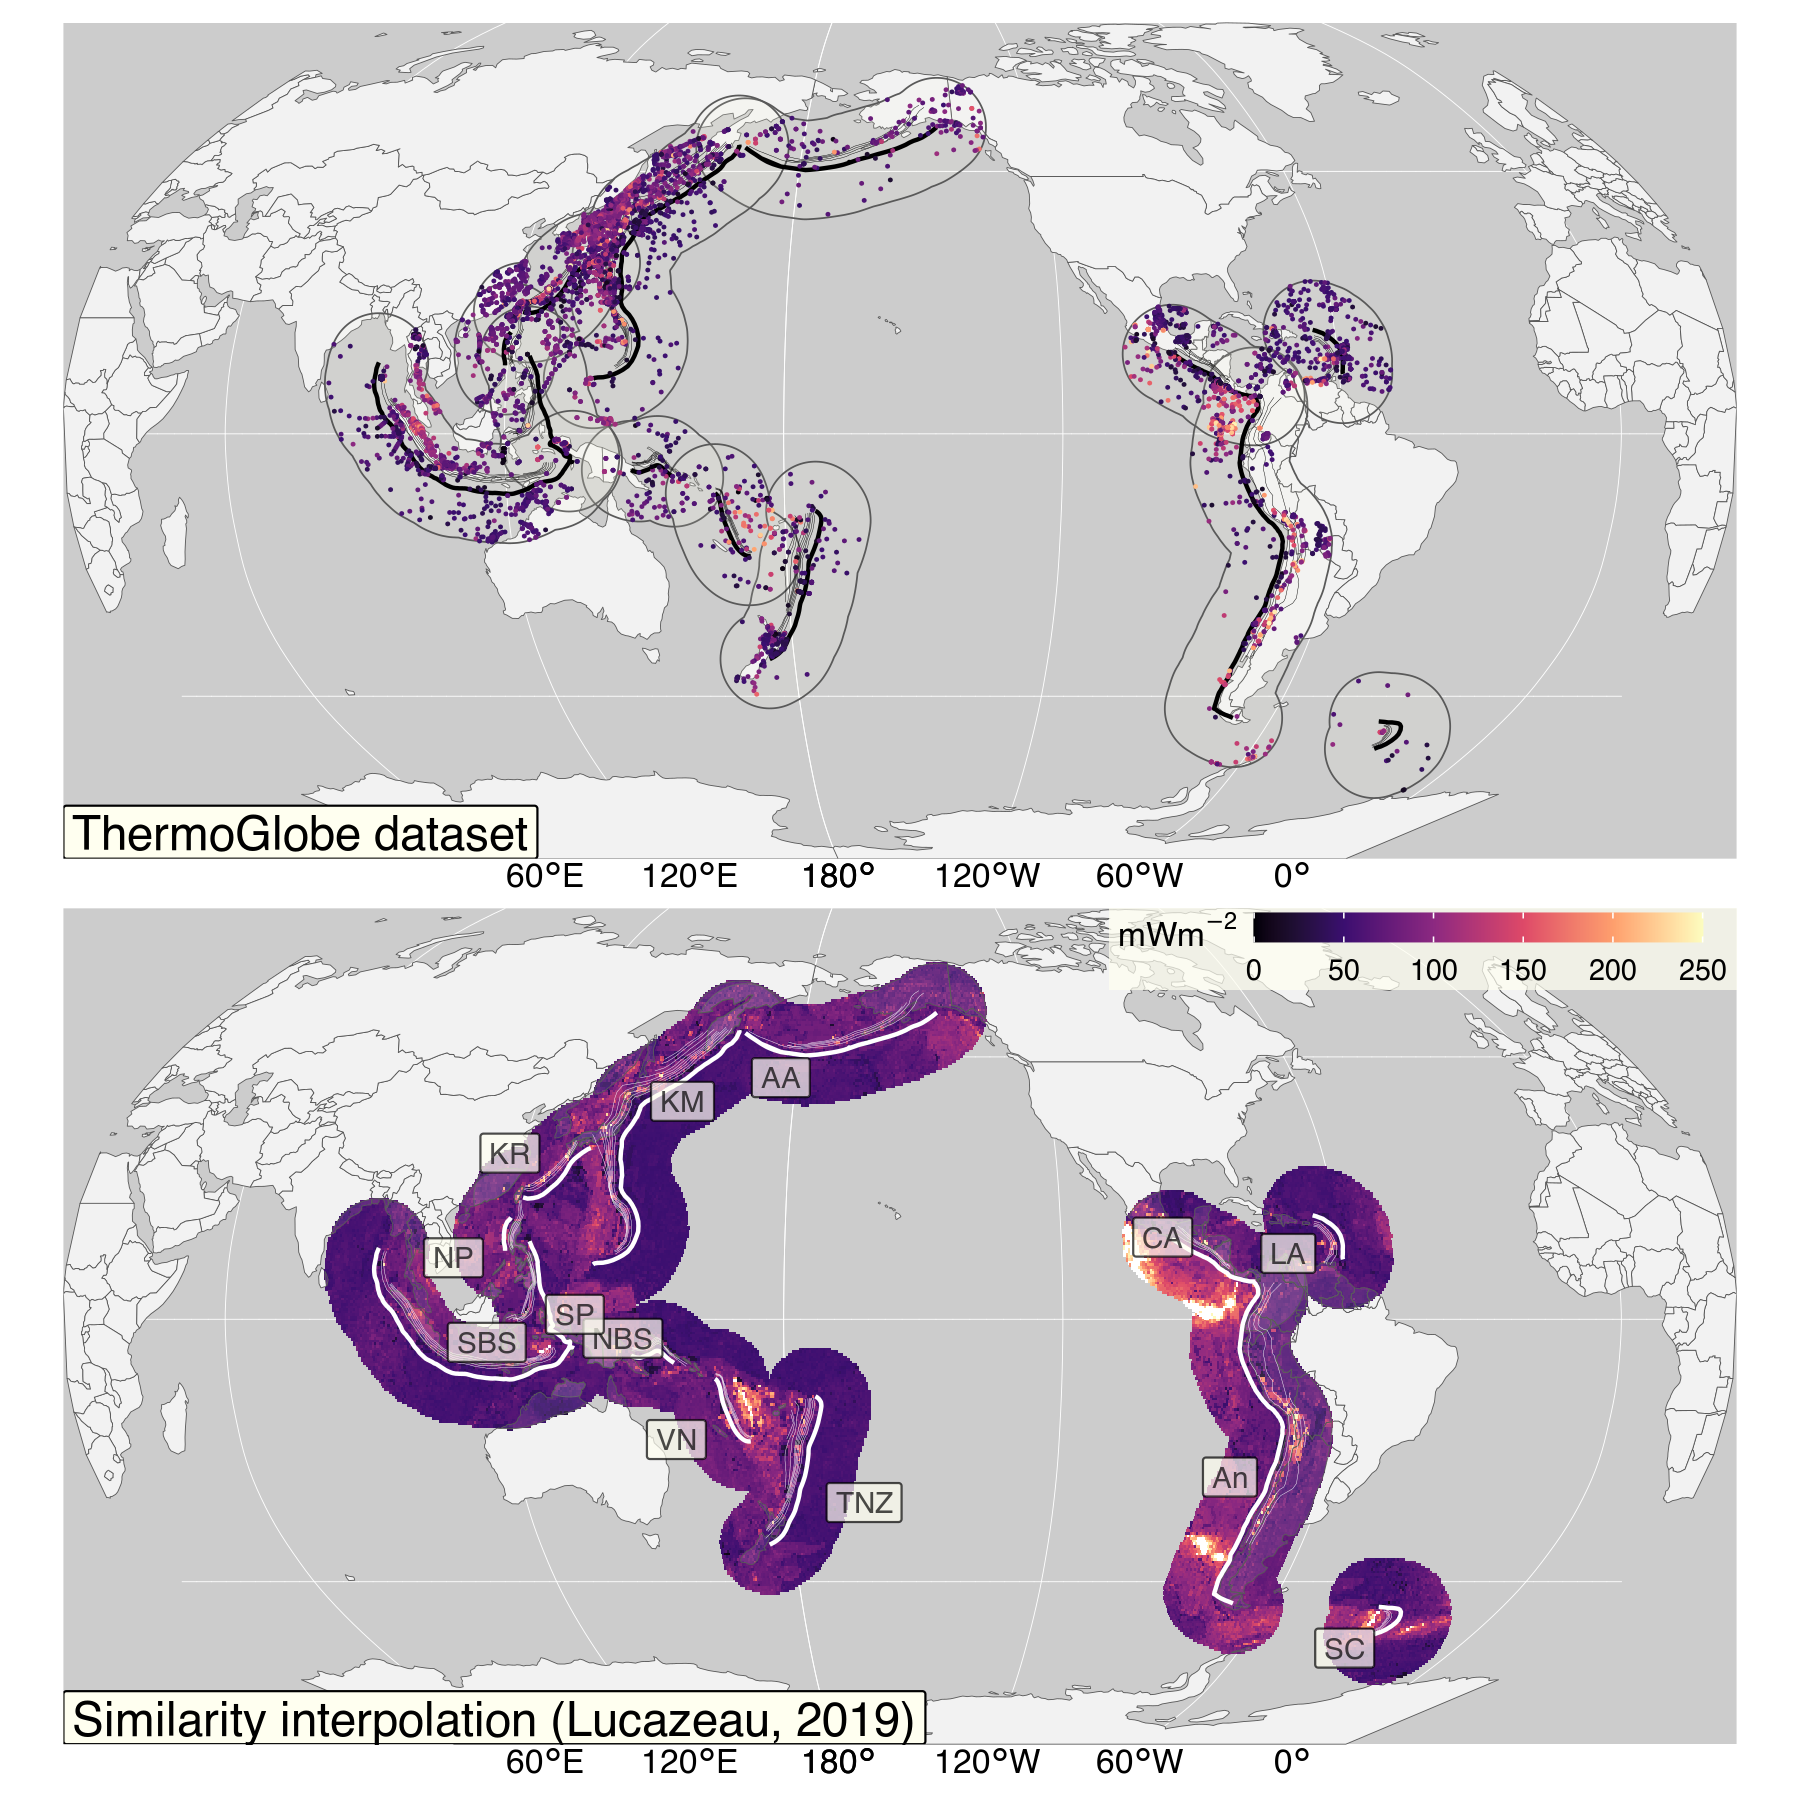
\includegraphics[width=1\linewidth,]{assets/figs/chpt3/ThermoGlobeBufferComp} 

}

\caption[Similarity interpolation of near 13 active subduction zone segments]{Surface heat flow near subduction zone segments. (a) ThermoGlobe data from Lucazeau (\protect\hyperlink{ref-lucazeau2019}{2019}) cropped within 1000 \(km\)-radius circular buffers around 13 active subduction zone segments show uneven regional coverage. For example, note the relatively high observational density in the NW Pacific compared to other regions. (b) In contrast, Similarity interpolation cropped within the same buffers presents an evenly-distributed approximation of regional surface heat flow. Similarity interpolation from Lucazeau (\protect\hyperlink{ref-lucazeau2019}{2019}). Subduction zone boundaries (bold white lines) \DIFaddbeginFL \DIFaddFL{and volcanoes (gold diamonds) }\DIFaddendFL defined by Syracuse \& Abers (\protect\hyperlink{ref-syracuse2006}{2006}). Plate boundaries (\DIFdelbeginFL \DIFdelFL{solid green }\DIFdelendFL \DIFaddbeginFL \DIFaddFL{bold black }\DIFaddendFL lines) defined by Lawver et al. (\protect\hyperlink{ref-lawver2018}{2018}). \DIFdelbeginFL \DIFdelFL{Segments: }\DIFdelendFL AA\DIFdelbeginFL %DIFDELCMD < {[}%%%
\DIFdelendFL \DIFaddbeginFL \DIFaddFL{: }\DIFaddendFL Alaska Aleutians\DIFdelbeginFL %DIFDELCMD < {]}%%%
\DIFdelendFL , AN\DIFdelbeginFL %DIFDELCMD < {[}%%%
\DIFdelendFL \DIFaddbeginFL \DIFaddFL{: }\DIFaddendFL Andes\DIFdelbeginFL %DIFDELCMD < {]}%%%
\DIFdelendFL , CA\DIFdelbeginFL %DIFDELCMD < \protect\hyperlink{central-america}{Central America}%%%
\DIFdelendFL \DIFaddbeginFL \DIFaddFL{: Central America}\DIFaddendFL , KM\DIFdelbeginFL %DIFDELCMD < {[}%%%
\DIFdelendFL \DIFaddbeginFL \DIFaddFL{: }\DIFaddendFL Kamchatka Marianas\DIFdelbeginFL %DIFDELCMD < {]}%%%
\DIFdelendFL , KR\DIFdelbeginFL %DIFDELCMD < \protect\hyperlink{kyushu-ryukyu}{Kyushu Ryukyu}%%%
\DIFdelendFL \DIFaddbeginFL \DIFaddFL{: Kyushu Ryukyu}\DIFaddendFL , LA\DIFdelbeginFL %DIFDELCMD < {[}%%%
\DIFdelendFL \DIFaddbeginFL \DIFaddFL{: }\DIFaddendFL Lesser Antilles\DIFdelbeginFL %DIFDELCMD < {]}%%%
\DIFdelendFL , NBS\DIFdelbeginFL %DIFDELCMD < {[}%%%
\DIFdelendFL \DIFaddbeginFL \DIFaddFL{: }\DIFaddendFL New Britain Solomon\DIFdelbeginFL %DIFDELCMD < {]}%%%
\DIFdelendFL , NP\DIFdelbeginFL %DIFDELCMD < {[}%%%
\DIFdelendFL \DIFaddbeginFL \DIFaddFL{: }\DIFaddendFL N Philippines\DIFdelbeginFL %DIFDELCMD < {]}%%%
\DIFdelendFL , SBS\DIFdelbeginFL %DIFDELCMD < {[}%%%
\DIFdelendFL \DIFaddbeginFL \DIFaddFL{: }\DIFaddendFL Sumatra Banda Sea\DIFdelbeginFL %DIFDELCMD < {]}%%%
\DIFdelendFL , SC\DIFdelbeginFL %DIFDELCMD < \protect\hyperlink{scotia}{Scotia}%%%
\DIFdelendFL \DIFaddbeginFL \DIFaddFL{: Scotia}\DIFaddendFL , SP\DIFdelbeginFL %DIFDELCMD < {[}%%%
\DIFdelendFL \DIFaddbeginFL \DIFaddFL{: }\DIFaddendFL S Philippines\DIFdelbeginFL %DIFDELCMD < {]}%%%
\DIFdelendFL , TNZ\DIFdelbeginFL %DIFDELCMD < {[}%%%
\DIFdelendFL \DIFaddbeginFL \DIFaddFL{: }\DIFaddendFL Tonga New Zealand\DIFdelbeginFL %DIFDELCMD < {]}%%%
\DIFdelendFL , VN\DIFdelbeginFL %DIFDELCMD < {[}%%%
\DIFdelendFL \DIFaddbeginFL \DIFaddFL{: }\DIFaddendFL Vanuatu\DIFdelbeginFL %DIFDELCMD < {]}%%%
\DIFdelendFL .}\label{fig:globalhfComp}
\end{figure}

In one class of methods (including Kriging), interpolation involves adjusting certain model parameters that depend on the relative positions of examples and targets. Because model parameters are spatially dependent, these methods inherently attempt to conserve the spatial continuity of observed surface heat flow. Kriging, therefore, predicts a more accurate (or truthful) \emph{on-the-ground} distribution of surface heat flow compared to Similarity methods (described below). The rationale for using Kriging is embodied in the First Law of Geography: \emph{everything is related, but nearer things are more related} (\protect\hyperlink{ref-krige1951}{Krige, 1951}; \protect\hyperlink{ref-matheron1963}{Matheron, 1963}).

However, ordinary Kriging must satisfy a condition known as \emph{second order weak stationarity}. That is, the relationship among surface heat flow observations is constant and only depends on the relative separation (lag) distance between pairs of observations. This assumption may be violated within tectonically-diverse regions where the underlying geodynamics may quickly transition from subduction to spreading centers, for example. However, stationarity need only apply over the local Kriging domain, so stationarity can be maintained by careful choice of Kriging parameters. Although not necessary in this study, stationarity assumptions can relax and other techniques that respect the Second Law of Geography (\emph{spatial phenomena are inherently heterogeneous}, \protect\hyperlink{ref-goodchild2004}{Goodchild, 2004}), such as directional Kriging or Markov-Bayes techniques (\protect\hyperlink{ref-bardossy1997}{Bárdossy, 1997}), can be applied.

In stark contrast to Kriging, Similarity methods are spatially independent and predict surface heat flow by integrating geographic, geologic, geochronologic, and geophysical information (see \protect\hyperlink{ref-goutorbe2011}{Goutorbe et al., 2011} for method details). The technique involves evaluating the number of similar observable geologic proxies between a target and \emph{every} example in the entire global dataset (e.g.~a target and an example are similar if they have similar bathymetry, elevation, proximity to active or ancient orogens, seafloor age, upper mantle shear wave velocities, etc., \protect\hyperlink{ref-chapman1975}{Chapman \& Pollack, 1975}; \protect\hyperlink{ref-davies2013}{Davies, 2013}; \protect\hyperlink{ref-lee1965}{Lee \& Uyeda, 1965}; \protect\hyperlink{ref-lucazeau2019}{Lucazeau, 2019}; \protect\DIFdelbegin %DIFDELCMD < \hyperlink{ref-sclater1970}{Sclater \& Francheteau, 1970}%%%
\DIFdelend \DIFaddbegin \hyperlink{ref-sclater1970}{Sclater et al., 1970a}\DIFaddend ; \protect\hyperlink{ref-shapiro2004}{Shapiro \& Ritzwoller, 2004}). Surface heat flow is then predicted at a target location as a function of the target's similarity with each example and the surface heat flow observed at each example, irrespective of their locations. Global-scale problems and regional domains with relatively few surface heat flow data are particularly suited for Similarity as the method is independent of observational density. The rationale for using Similarity is embodied in the Third Law of Geography: \emph{the more similar the geographic configuration of two points, the more similar their values} (\protect\hyperlink{ref-zhu2018}{Zhu et al., 2018}).

However, it is especially notable for regional geodynamic investigations that Kriging is explicitly spatially dependent, whereas Similarity is not. Generally speaking, spatial (dis)continuity of surface heat flow observations reflect the (dis)continuity of subsurface geodynamics (assuming insignificant near-surface perturbations). For example, broad regions of low surface heat flow on continents outline cratons and repeated surface heat flow patterns near subduction zones are interpreted to reflect uniform upper-plate lithospheric thickness (\protect\hyperlink{ref-currie2004}{Currie et al., 2004}; \protect\hyperlink{ref-currie2006}{Currie \& Hyndman, 2006}; \protect\hyperlink{ref-hyndman2005}{Hyndman et al., 2005}) and mechanical coupling depths (\protect\hyperlink{ref-furukawa1993}{Furukawa, 1993}; \protect\hyperlink{ref-kerswell2020}{Kerswell et al., 2020}; \protect\hyperlink{ref-wada2009}{Wada \& Wang, 2009}). While Similarity may be accurate in many cases, simply imposing surface heat flow by layering geologic proxies without explicitly considering the spatial continuity of surface heat flow observations is concerning for at least two reasons. It may 1) discount random unpredictable subsurface geodynamics, and/or 2) discount random unpredictable near-surface perterbations. Either case leads to erroneous surface heat flow inversions and interpretations of subsurface geodynamics. It is therefore crucial for regional geodynamic investigations to characterize the true spatial continuity of surface heat flow observations whenever possible.

This Chapter compares surface heat flow interpolations produced by Similarity and Kriging methods for 13 presently active subduction zones while considering the following questions. How does surface heat flow vary in 2D near subduction zones, especially along strike within upper-plates? Are Kriging and Similarity methods comparable when applied to surface heat flow near subduction zones? What do the differences (if any) imply about geodynamic variability among active subduction zones, especially with respect to uniform upper-plate thickness discussed in Chapter \ref{chpt2}?

First, ordinary Kriging is applied to the ThermoGlobe dataset (\protect\hyperlink{ref-jennings2021}{Jennings \& Hasterok, 2021}; \protect\hyperlink{ref-lucazeau2019}{Lucazeau, 2019}) cropped within 1000 \(km\)-radius circular buffers around 13 presently active subduction zones defined by Syracuse \& Abers (\protect\hyperlink{ref-syracuse2006}{2006}). Kriging predictions are then directly compared (point-by-point) to Similarity interpolations from a previous global-scale study by Lucazeau (\protect\hyperlink{ref-lucazeau2019}{2019}). The results show Kriging and Similarity methods are grossly comparable at regional scales (\(\geq\) 100's of \(km\)), but more importantly, show distinct differences in upper-plate surface heat flow for 7 out of 13 subduction zone segments. Average upper-plate surface heat flow can vary up to 50 \(mWm^{-2}\) across a single subduction zone segment---implying non-uniform upper-plate thickness in contradiction to expectations from Chapter \ref{chpt2}. More subtle differences between Kriging and Similarity results point to inherent methodological strengths that may be combined in layered interpolation methods.

\hypertarget{chpt3Methods}{%
\section{Methods}\label{chpt3Methods}}

\hypertarget{the-thermoglobe-database}{%
\subsection{The ThermoGlobe Database}\label{the-thermoglobe-database}}

The ThermoGlobe database is available from the supplementary material of Lucazeau (\protect\hyperlink{ref-lucazeau2019}{2019}) and is accessible online at \url{http://heatflow.org} (\protect\hyperlink{ref-jennings2021}{Jennings \& Hasterok, 2021}). It currently contains 69,729 data points, their locations in latitude/longitude, and important metadata---including a data quality rank (\texttt{Code\ 6}) from A (high-quality) to D (low-quality). The reader is referred to Lucazeau (\protect\hyperlink{ref-lucazeau2019}{2019}) and \url{http://heatflow.org} for details on compilation, references, historical perspective on ThermoGlobe, and previous compilations. ThermoGlobe is the most recent database available, has been carefully compiled, and is open-access.

Like Lucazeau (\protect\hyperlink{ref-lucazeau2019}{2019}), 4,661 poor quality observations (\texttt{Code\ 6} = D), 350 data points without heat flow observations, and 2 without geographic information are excluded from the analysis. Note that quality control of such a large dataset is an ongoing endeavor and 11,712 observations currently have an undetermined quality (\texttt{Code\ 6} = Z). Duplicate observations at the same location are parsed (to avoid singular covariance matrices during Kriging) by selecting only the best quality measurement. If duplicate measurements are of equal quality, one is randomly chosen. Finally, only surface heat flow observations in the range (0 - 250{]} \(mWm^{-2}\) are included in Kriging. Similarity interpolations from Lucazeau (\protect\hyperlink{ref-lucazeau2019}{2019}) is also limited to the range (0 - 250{]} \(mWm^{-2}\). Observations outside of the range (0 - 250{]} \(mWm^{-2}\) are considered anomalous (e.g.~collected near geothermal systems, \protect\hyperlink{ref-lucazeau2019}{Lucazeau, 2019}) and constitute a small fraction of measurements (4,883 out of 69,729) forming long tails on either side of the global surface heat flow distribution. The final dataset used for Kriging contains 13,368 observations after filtering for quality, missing values, and heat flow range, parsing duplicate pairs, and cropping within subduction zone buffers (\DIFdelbegin \DIFdel{Table \ref{tab:hfSummaryTable} \& Figure \ref{fig:hfSummaryPlot} }\DIFdelend \DIFaddbegin \DIFadd{Figure \ref{fig:hfSummaryPlot} \& Table \ref{tab:hfSummaryTable}}\DIFaddend ).

\hypertarget{map-projection-and-interpolation-grid}{%
\subsection{Map Projection and Interpolation Grid}\label{map-projection-and-interpolation-grid}}

All geographic operations, including transformation, cropping, Kriging, and comparing interpolations, are performed using general-purpose functions in the \texttt{R} package \texttt{sf} (\protect\hyperlink{ref-pebesma2018}{Pebesma, 2018}). ThermoGlobe data and Similarity interpolations from Lucazeau (\protect\hyperlink{ref-lucazeau2019}{2019}) are transformed into a Pacific-centered Robinson coordinate reference system using the open source geographic transformation software \texttt{PROJ} (\protect\hyperlink{ref-proj2021}{PROJ contributors, 2021}). The transformation is defined by the \texttt{proj4} string \texttt{"+proj=robin\ +lon\_0=-155\ +lon\_wrap=-155\ +x\_0=0\ +y\_0=0\ +ellps=WGS84\ +datum=WGS84\ +units=m\ +no\_defs"}. The Kriging domains \DIFdelbegin \DIFdel{(Figure \ref{fig:domainConstruct}) }\DIFdelend are defined by drawing 1000 \(km\)-radius circular buffers around each subduction zone segment defined by Syracuse \& Abers (\protect\hyperlink{ref-syracuse2006}{2006}). Target locations for Kriging \DIFaddbegin \DIFadd{(the interpolation grid) }\DIFaddend are defined across the same grid used by Lucazeau (\protect\hyperlink{ref-lucazeau2019}{2019}) to compute point-by-point differences with their Similarity interpolation \DIFdelbegin \DIFdel{.
}\DIFdelend \DIFaddbegin \DIFadd{(Figure \ref{fig:domainConstruct}). In this case, grid point locations represent the centroids of 0.5\(^\circ \times\) 0.5\(^\circ\) unequal-area grid cells encompassing the entire globe.
}\DIFaddend 



\begin{figure}[htbp]

{\centering \DIFdelbeginFL %DIFDELCMD < 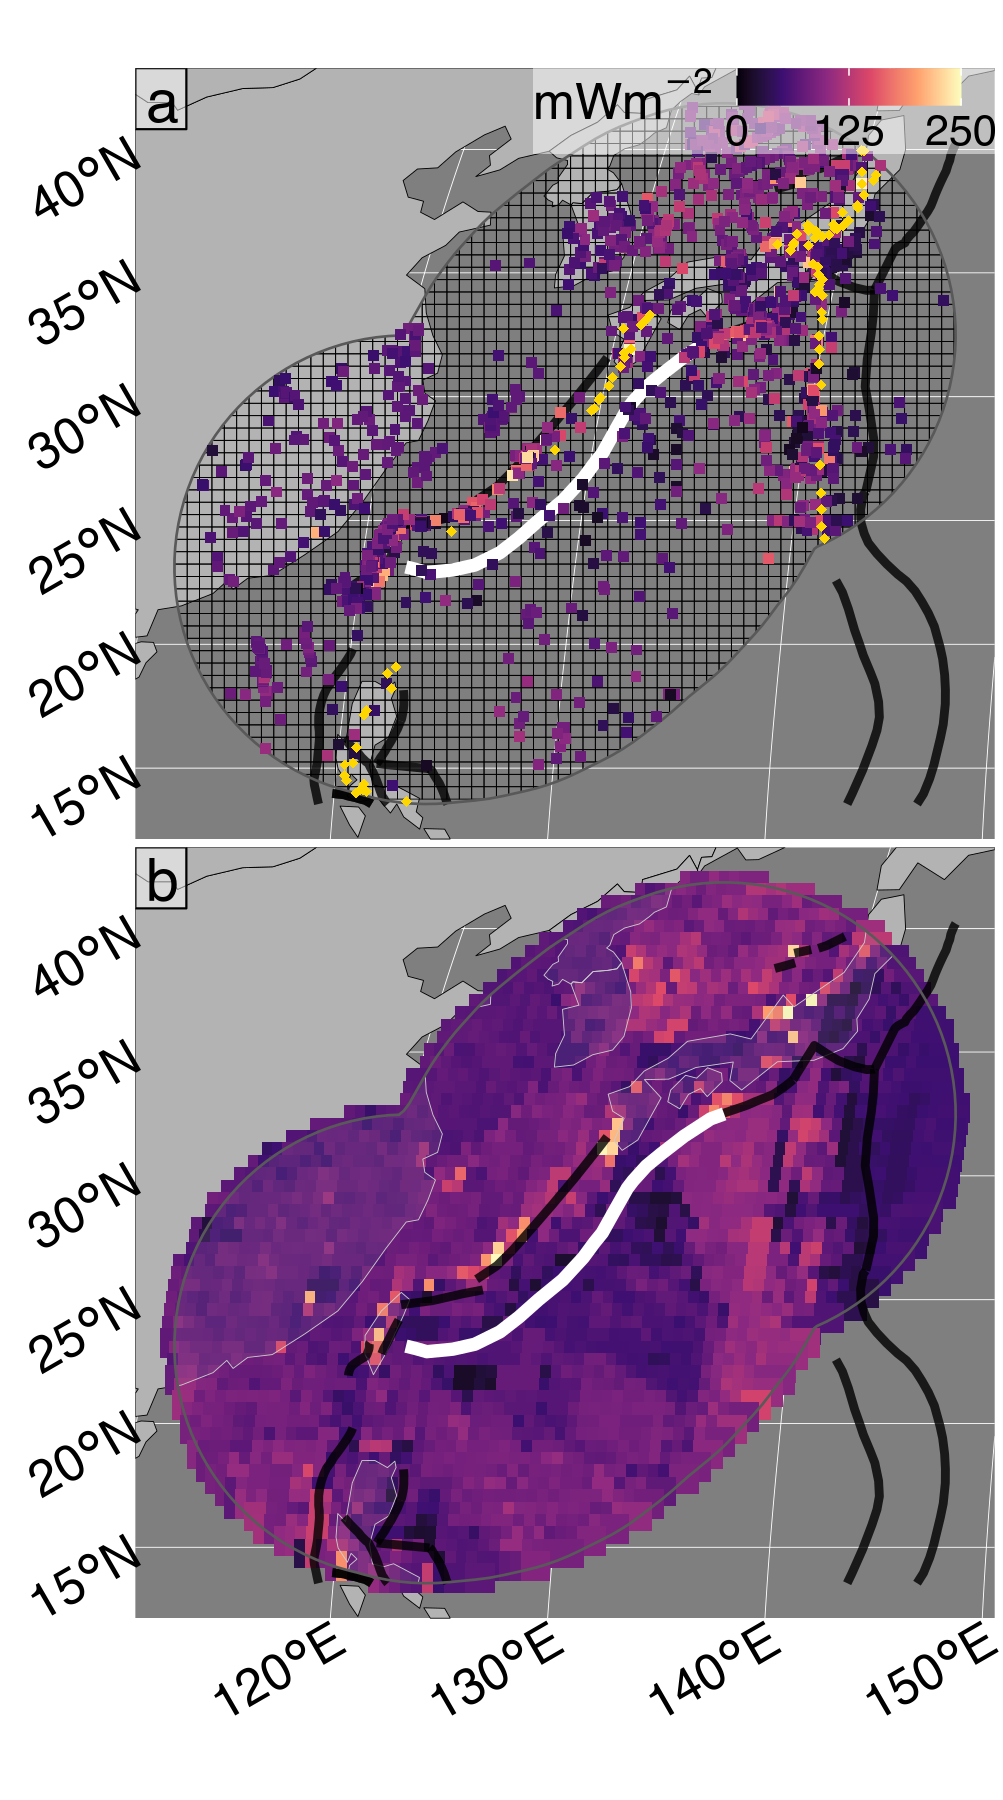
\includegraphics[width=0.6\linewidth,]{assets/figs/chpt3/KyushuRyukyuComp} 
%DIFDELCMD < %%%
\DIFdelendFL \DIFaddbeginFL 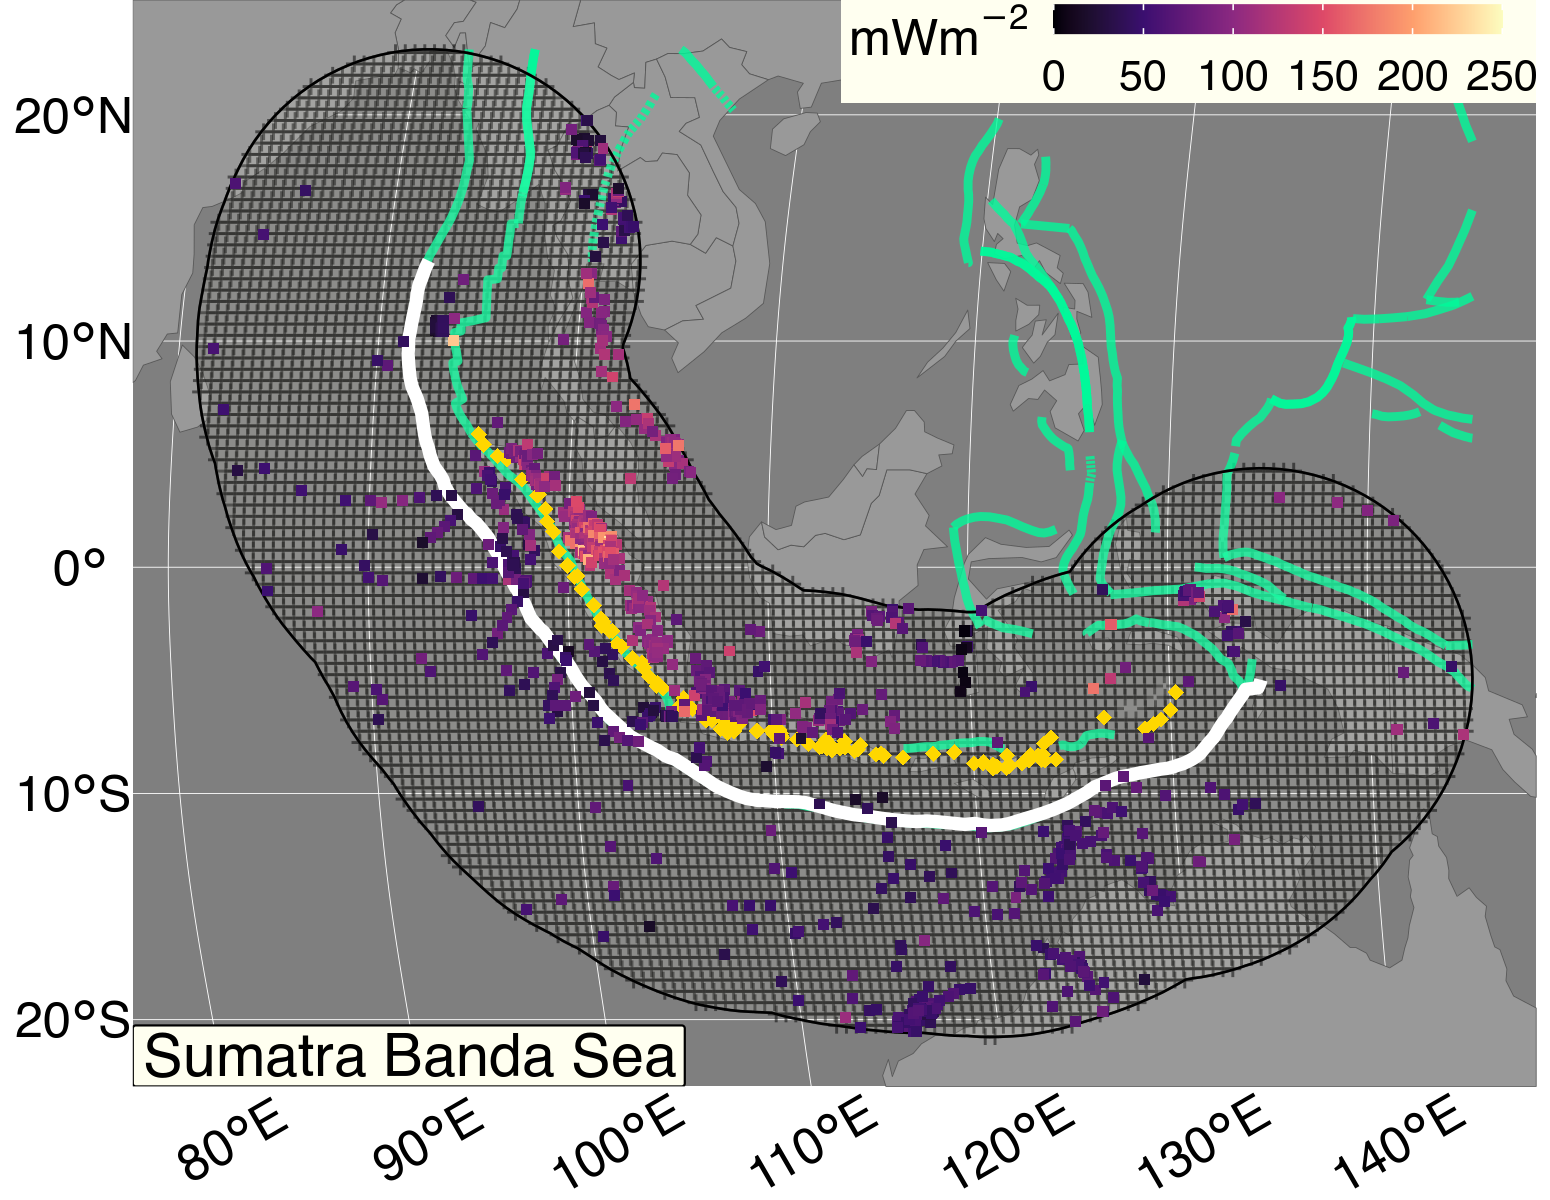
\includegraphics[width=1\linewidth,]{assets/figs/chpt3/SumatraBandaSeaInterp} 
\DIFaddendFL 

}

\DIFdelbeginFL %DIFDELCMD < \caption[Example of an interpolation domain constructed around Kyushu Ryukyu]{%%%
\DIFdelendFL \DIFaddbeginFL \caption[Example of an interpolation domain constructed around Sumatra Banda Sea]{\DIFaddendFL Example of an interpolation domain constructed around \DIFdelbeginFL \DIFdelFL{Kyushu Ryukyu}\DIFdelendFL \DIFaddbeginFL \DIFaddFL{Sumatra Banda Sea}\DIFaddendFL . \DIFdelbeginFL \DIFdelFL{(a) }\DIFdelendFL ThermoGlobe data \DIFaddbeginFL \DIFaddFL{(colored squares, }\protect\hyperlink{ref-lucazeau2019}{Lucazeau, 2019}\DIFaddFL{) }\DIFaddendFL are cropped within a \DIFdelbeginFL \DIFdelFL{domain defined by drawing a }\DIFdelendFL 1000 \(km\)-radius circular buffer (thin black line) \DIFdelbeginFL \DIFdelFL{around }\DIFdelendFL \DIFaddbeginFL \DIFaddFL{surrounding }\DIFaddendFL the segment boundary (bold white line). \DIFaddbeginFL \DIFaddFL{Target locations for interpolation are defined by the intersections of a 0.5\(^\circ \times\) 0.5\(^\circ\) grid (fine black mesh, defined by }\protect\hyperlink{ref-lucazeau2019}{Lucazeau, 2019}\DIFaddFL{) cropped to the same buffer. }\DIFaddendFL Note that \DIFdelbeginFL \DIFdelFL{Kyushu Ryukyu }\DIFdelendFL \DIFaddbeginFL \DIFaddFL{Sumatra Banda Sea }\DIFaddendFL is one of the most \DIFdelbeginFL \DIFdelFL{densely }\DIFdelendFL sampled regions, yet still has considerable observational gaps. \DIFdelbeginFL \DIFdelFL{(b) Similarity presents a textured interpolation by layering many geologic proxy datasets. Similarity interpolation from Lucazeau (}%DIFDELCMD < \protect\hyperlink{ref-lucazeau2019}{2019}%%%
\DIFdelFL{). }\DIFdelendFL Segment boundary \DIFaddbeginFL \DIFaddFL{and volcanoes (gold diamonds) }\DIFaddendFL defined by Syracuse \& Abers (\protect\hyperlink{ref-syracuse2006}{2006}). Plate boundaries (\DIFdelbeginFL \DIFdelFL{solid green }\DIFdelendFL \DIFaddbeginFL \DIFaddFL{bold black }\DIFaddendFL lines) defined by Lawver et al. (\protect\hyperlink{ref-lawver2018}{2018}).}\label{fig:domainConstruct}
\end{figure}

\hypertarget{kriging}{%
\subsection{Kriging}\label{kriging}}

Kriging is derived from the theory of \emph{regionalized variables} (\protect\hyperlink{ref-matheron1963}{Matheron, 1963}, \protect\hyperlink{ref-matheron2019}{2019}) and approximates an unknown quantity as a linear combination of all nearby known quantities. Kriging is a three-step process that involves: 1) estimating an experimental variogram \(\hat{\gamma}(h)\) that characterizes the spatial (dis)continuity of some quantity within the Kriging domain, 2) fitting one of many variogram models \(\gamma(h)\) to the experimental variogram, and 3) directly solving a linear system of Kriging equations to predict unknown quantities at arbitrary target locations (\protect\hyperlink{ref-cressie2015}{Cressie, 2015}; \protect\hyperlink{ref-krige1951}{Krige, 1951}). The general-purpose functions defined in the \texttt{R} package \texttt{gstat} (\protect\hyperlink{ref-graler2016}{Gräler et al., 2016}; \protect\hyperlink{ref-pebesma2004}{Pebesma, 2004}) are used to perform all three Kriging steps. The first step is computing an experimental variogram (after \protect\hyperlink{ref-bardossy1997}{Bárdossy, 1997}):
\DIFdelbegin %DIFDELCMD < 

%DIFDELCMD < %%%
\DIFdelend \begin{equation}
  \DIFdelbegin %DIFDELCMD < \begin{aligned}
%DIFDELCMD <     &\hat{\gamma}(h) = \frac{1}{2N(h)}\sum_{N(h)}^{}[Z(u_i) - Z(u_j)]^2 \\
%DIFDELCMD <     &h = |u_i - u_j| \\
%DIFDELCMD <     &\delta = \frac{\max(h)\ (n_{lag}+l)}{n_{lag}\ c} \\
%DIFDELCMD <     &N(h) = \#\{h \  \in \  [h - \delta,\  h + \delta)\}
%DIFDELCMD <   \end{aligned}%%%
\DIFdelend \DIFaddbegin \begin{aligned}
    &\hat{\gamma}(h) = \frac{1}{2N(h)}\sum_{N(h)}^{}[Z(u_i) - Z(u_j)]^2 \\
    &h = |u_i - u_j| \\
  \end{aligned}\DIFaddend 
  \label{eq:variogram}
\end{equation}
\DIFdelbegin %DIFDELCMD < 

%DIFDELCMD < %%%
\DIFdelend \DIFaddbegin \DIFadd{where \(Z(u_i)\) and \(Z(u_j)\) are observations located at \(u_i\) and \(u_j\) separated by a lag of \(h\) and \(N(h)\) is the number of observations separated by a given lag distance. }\DIFaddend The experimental variogram \(\hat{\gamma}(h)\) evaluates the spatial continuity \DIFdelbegin \DIFdel{(or variability) }\DIFdelend of the set of observations \(Z(u)\) by computing the average variance among pairs of observations separated by increasingly greater \DIFdelbegin \DIFdel{``lag distances'' \(h\), or simply ``lags''}\DIFdelend \DIFaddbegin \DIFadd{lag distances}\DIFaddend . By convention the average variance \DIFdelbegin \DIFdel{among pairs of observations separated by some lag distance }\DIFdelend is halved and called ``semivariance'' \DIFdelbegin \DIFdel{. \(Z(u_i)\) and \(Z(u_j)\) are observations located at points \(u_i\) and \(u_j\) with a lag of \(h = u_i - u_j\). }\DIFdelend \DIFaddbegin \DIFadd{\(\hat{\gamma}(h)\).
}

\DIFaddend For regularly-spaced data, lag distances are simply multiples of the grid-step distance, but irregularly-spaced data must be treated differently. In the case of irregularly-spaced surface heat flow in this study, a binwidth \(\delta\) is defined as\DIFdelbegin \DIFdel{a function of }\DIFdelend \DIFaddbegin \DIFadd{:
}\begin{equation}
  \DIFadd{\begin{aligned}
    &\delta = \frac{\max(h)\ (n_{lag}+l)}{n_{lag}\ c} \\
    &N(h) = \#\{h \  \in \  [h - \delta,\  h + \delta)\}
  \end{aligned}
  \label{eq:binwidth}
}\end{equation}
\DIFadd{where \(\max(h)\) is }\DIFaddend the maximum separation distance within the Kriging domain\DIFdelbegin \DIFdel{\(\max(h)\), }\DIFdelend \DIFaddbegin \DIFadd{, \(n_{lag}\) is }\DIFaddend the number of lags used to evaluate the variogram\DIFdelbegin \DIFdel{\(n_{lag}\), }\DIFdelend \DIFaddbegin \DIFadd{, \(l\) is }\DIFaddend a lag shift constant \DIFdelbegin \DIFdel{\(l\) }\DIFdelend that shifts the variogram by an integer number of binwidths, \DIFdelbegin \DIFdel{and }\DIFdelend \DIFaddbegin \DIFadd{\(c\) is }\DIFaddend a lag cutoff constant \DIFdelbegin \DIFdel{\(c\) which is simply a fraction between 0 and 1 }\DIFdelend (by convention \DIFdelbegin \DIFdel{\(c=1/3\)). }\DIFdelend \DIFaddbegin \DIFadd{\(c=3\)). Then }\DIFaddend \(N(h)\) is the number of observations that fall within \DIFdelbegin \DIFdel{a lag distance with bindwidth \([h - \delta,\  h + \delta)\)}\DIFdelend \DIFaddbegin \DIFadd{\(h = [h-\delta,\ h+\delta)\)}\DIFaddend .

This study applies ordinary Kriging with isotropic variogram models (assumes semivariance is spatially invariant) to surface heat flow data projected onto a smooth sphere (neglects elevation). Kriging is applied locally (to avoid violating stationarity assumptions) by evaluating only the nearest \(n_{max}\) observations at each target location, where ``nearest'' is defined by the distances between the target location and observations. Therefore, the domain of local Kriging expands or shrinks depending on the local observational density at each target location.

Several variogram parameters influence the Kriging result, including the choice of variogram model, the scope of local Kriging \(n_{max}\), and choice of experimental variogram parameters in Equation \eqref{eq:variogram}. Instead of choosing Kriging parameters by eye (a common practice for fitting variograms) this study uses a constrained non-linear optimization approach to find optimum values for the parameters \(\{model,\ n,\ c,\ n_{max},\ l\}\). A weighted sum of variogram \gls{rmse} and Kriging \gls{rmse} is used as a cost function to simultaneously optimize variogram and Kriging accuracy (after \protect\hyperlink{ref-li2018}{Li et al., 2018}). The \texttt{R} package \texttt{nloptr} is used to optimize Kriging parameters by finding a combination of \(\{model,\ n,\ c,\ n_{max},\ l\}\) that minimizes the cost function\DIFdelbegin \DIFdel{(Table \ref{tab:vgrmSummaryTable})}\DIFdelend . A full description of the Kriging system of equations, underlying assumptions, and optimization methods is presented in Appendix \ref{krigeOpt} with optimization results for all segments and variogram models. All experimental and fitted variograms are presented in Appendix \ref{interpDiffAppendix} with interpolations for each case.

\hypertarget{upper-plate-sectors}{%
\subsection{Upper-plate Sectors}\label{upper-plate-sectors}}

\DIFdelbegin \DIFdel{Along strike variability in }\DIFdelend \DIFaddbegin \DIFadd{Surface heat flow profiles and distributions are computed for several adjacent }\DIFaddend upper-plate \DIFaddbegin \DIFadd{regions to assess lateral (along-strike) }\DIFaddend surface heat flow \DIFdelbegin \DIFdel{is computed by splitting each }\DIFdelend \DIFaddbegin \DIFadd{variability. Profiles are defined by (1) splitting a }\DIFaddend subduction zone segment \DIFdelbegin \DIFdel{into 4-6 partsof equal length. Next, }\DIFdelend \DIFaddbegin \DIFadd{(defined by }\protect\hyperlink{ref-syracuse2006}{Syracuse \& Abers, 2006}\DIFadd{) into 2-8 equidistant parts, (2) defining }\DIFaddend 500 \(km\)-wide single-sided buffers (sectors) \DIFdelbegin \DIFdel{are defined for each segment part. Then, }\DIFdelend \DIFaddbegin \DIFadd{around the segment parts, and (3) calculating }\DIFaddend the orthogonal great circle distance between each surface heat flow prediction \DIFaddbegin \DIFadd{(Similarity and Kriging), or observation (ThermoGlobe data), contained }\DIFaddend within a sector and \DIFdelbegin \DIFdel{the subduction zone segment are computed. Plotting distance vs.~}\DIFdelend \DIFaddbegin \DIFadd{its part of the segment boundary (trench). Steps (1-3) above closely approximate the 2D distribution of }\DIFaddend surface heat flow \DIFdelbegin \DIFdel{is approximately equivalent to projecting surface heat flow predictions within a sector onto a line extending orthogonally from }\DIFdelend \DIFaddbegin \DIFadd{projected onto a 1D trench-orthogonal line at }\DIFaddend the center of \DIFdelbegin \DIFdel{each subduction zone segment part (c.f}\DIFdelend \DIFaddbegin \DIFadd{a sector (e.g}\DIFaddend ., \protect\hyperlink{ref-currie2004}{Currie et al., 2004}; \protect\hyperlink{ref-currie2006}{Currie \& Hyndman, 2006}; \protect\hyperlink{ref-hyndman2005}{Hyndman et al., 2005}; \protect\hyperlink{ref-wada2009}{Wada \& Wang, 2009}). \DIFdelbegin \DIFdel{Upper-plate surface heat flow oscillations orthogonal to the segment boundary }\DIFdelend \DIFaddbegin \DIFadd{Profiles }\DIFaddend are smoothed by \DIFdelbegin \DIFdel{computing a running average with }\DIFdelend a \DIFdelbegin \DIFdel{five-point binwidth, then fitting a curve to the running average using a local regression approach (LOESS, }\DIFdelend \DIFaddbegin \DIFadd{three-point running average and fit with a local non-parametric regression curve (LOESS, }\DIFaddend \protect\DIFdelbegin %DIFDELCMD < \hyperlink{ref-cleavland1988}{\textbf{cleavland1988?}}%%%
\DIFdel{).
}\DIFdelend \DIFaddbegin \hyperlink{ref-cleveland1988}{Cleveland \& Devlin, 1988}\DIFadd{).
}\DIFaddend 

\DIFaddbegin \hypertarget{similarity-accuracy}{%
\subsection{Similarity Accuracy}\label{similarity-accuracy}}

\DIFadd{Previous studies evaluate global Similarity prediction accuracy by applying leave-one-out cross-validation during the interpolation process (}\protect\hyperlink{ref-goutorbe2011}{Goutorbe et al., 2011}\DIFadd{) or directly computing }\gls{rmse} \DIFadd{after interpolation (}\protect\hyperlink{ref-lucazeau2019}{Lucazeau, 2019}\DIFadd{). This study evaluates Similarity accuracy with a direct approach (similar to }\protect\hyperlink{ref-lucazeau2019}{Lucazeau, 2019}\DIFadd{) because of its simplicity, robustness, and ease of implementation compared to cross-validation. The direct approach involves evaluating }\gls{rmse} \DIFadd{between Similarity predictions and surface heat flow observations at the same location. This requires either (1) interpolating nearby Similarity predictions onto locations with ThermoGlobe data, (2) interpolating nearby ThermoGlobe data onto the 0.5\(^\circ \times\) 0.5\(^\circ\) interpolation grid defined by Lucazeau (}\protect\hyperlink{ref-lucazeau2019}{2019}\DIFadd{), or (3) interpolate Similarity predictions and ThermoGlobe data onto any other arbitrary point. This study interpolates ThermoGlobe data onto grid points (option 2) as a weighted average of all surface heat flow observations found within a 55 \(km\) radius (approximately 0.5\(^\circ\) radius circle at the equator). However, instead of applying equal weights (arithmetic mean) as Lucazeau (}\protect\hyperlink{ref-lucazeau2019}{2019}\DIFadd{), this study applies an inverse weighted distance method defined as (after }\protect\hyperlink{ref-shepard1968}{Shepard, 1968}\DIFadd{):
}\begin{equation}
  \DIFadd{\begin{aligned}
    Z(u_c) &=
    \begin{cases}
      \ \frac{\sum_{i=1}^N \omega_i\ Z(u_i)}{\sum_{i=1}^N \omega_i} \quad \text{if } d(u_i,\ u_c) \neq 0 \text{ for all } i \\
      \ u_i \quad \quad \quad \quad \quad \text{if }  d(u_i,\ u_c) = 0 \text{ for some } i
    \end{cases} \\
    \omega_i &= \frac{1}{d(u_i,\ u_c)^p}
  \end{aligned}
  \label{eq:idw}
}\end{equation}
\DIFadd{where \(Z(u_c)\) is the expected surface heat flow at a grid point \(u_c\), \(Z(u_i)\) is the surface heat flow observed at location \(u_i\), \(N\) is the number of observations contained within 55 \(km\) (approximately 0.5\(^\circ\)) of the grid point, \(\omega_i\) is the weight applied to \(Z(u_i)\), \(d(u_i, u_c)\) is a function measuring the distance between observation location \(u_i\) and grid point \(u_c\), and \(p=2\) is a power constant affecting the smoothness of the interpolation. Finally, Similarity accuracy is evaluated by directly computing }\gls{rmse} \DIFadd{at the set of all grid points with interpolated ThermoGlobe data.
}

\DIFaddend \hypertarget{chpt3Results}{%
\section{Results}\label{chpt3Results}}

\hypertarget{optimum-kriging-parameters}{%
\subsection{Optimum Kriging Parameters}\label{optimum-kriging-parameters}}

Optimized Kriging parameters vary substantially from segment to segment (Table \ref{tab:vgrmSummaryTable}). However, despite a range of domain sizes, observational densities, and diverse \DIFdelbegin \DIFdel{tectonic }\DIFdelend \DIFaddbegin \DIFadd{plate }\DIFaddend configurations, Kriging parameters converge on solutions for all Kriging domains (Figure \ref{fig:optTrace}) and show no systematic correlation with cost (Figure \ref{fig:vgrmSummaryPlot}). Differences in cost are apparently explained by systematic regional differences in surface heat flow distributions (i.e.~differences in the constant terms \(\sigma_{vgrm}\) and \(\sigma_{interp}\) in Equation \eqref{eq:costExp}) rather than sensitivity to Kriging parameters.

\begin{table}

\caption{\label{tab:vgrmSummaryTable}Optimum variogram models \DIFaddbeginFL \DIFaddFL{and interpolation accuracy }\DIFaddendFL by segment}
\centering
\DIFdelbeginFL %DIFDELCMD < \resizebox{\linewidth}{!}{
%DIFDELCMD < \begin{threeparttable}
%DIFDELCMD < \begin{tabular}[t]{llrrrrrrr}
%DIFDELCMD < \toprule
%DIFDELCMD < Segment & Model & Cutoff & Lags & Shift & $n_{max}$ & Sill & Range & Cost\\
%DIFDELCMD < \midrule
%DIFDELCMD < \cellcolor{gray!6}{Alaska Aleutians} & \cellcolor{gray!6}{Lin} & \cellcolor{gray!6}{1.0} & \cellcolor{gray!6}{15.0} & \cellcolor{gray!6}{1.6} & \cellcolor{gray!6}{10.0} & \cellcolor{gray!6}{824} & \cellcolor{gray!6}{258} & \cellcolor{gray!6}{0.647}\\
%DIFDELCMD < Andes & Exp & 7.3 & 24.8 & 1.6 & 11.9 & 2575 & 12 & 0.306\\
%DIFDELCMD < \cellcolor{gray!6}{Central America} & \cellcolor{gray!6}{Cir} & \cellcolor{gray!6}{13.0} & \cellcolor{gray!6}{24.7} & \cellcolor{gray!6}{1.3} & \cellcolor{gray!6}{11.2} & \cellcolor{gray!6}{2038} & \cellcolor{gray!6}{10} & \cellcolor{gray!6}{0.262}\\
%DIFDELCMD < Kamchatka Marianas & Sph & 1.0 & 17.3 & 2.1 & 11.2 & 1799 & 814 & 0.426\\
%DIFDELCMD < \cellcolor{gray!6}{Kyushu Ryukyu} & \cellcolor{gray!6}{Lin} & \cellcolor{gray!6}{1.0} & \cellcolor{gray!6}{20.5} & \cellcolor{gray!6}{1.5} & \cellcolor{gray!6}{31.9} & \cellcolor{gray!6}{1873} & \cellcolor{gray!6}{119} & \cellcolor{gray!6}{0.484}\\
%DIFDELCMD < Lesser Antilles & Sph & 2.9 & 27.2 & 1.5 & 29.0 & 782 & 141 & 0.310\\
%DIFDELCMD < \cellcolor{gray!6}{N Philippines} & \cellcolor{gray!6}{Lin} & \cellcolor{gray!6}{1.3} & \cellcolor{gray!6}{15.4} & \cellcolor{gray!6}{1.6} & \cellcolor{gray!6}{14.2} & \cellcolor{gray!6}{1206} & \cellcolor{gray!6}{66} & \cellcolor{gray!6}{0.541}\\
%DIFDELCMD < New Britain Solomon & Lin & 13.1 & 22.6 & 1.6 & 10.0 & 806 & 65 & 0.790\\
%DIFDELCMD < \cellcolor{gray!6}{S Philippines} & \cellcolor{gray!6}{Bes} & \cellcolor{gray!6}{13.1} & \cellcolor{gray!6}{23.5} & \cellcolor{gray!6}{1.5} & \cellcolor{gray!6}{10.0} & \cellcolor{gray!6}{849} & \cellcolor{gray!6}{5} & \cellcolor{gray!6}{0.498}\\
%DIFDELCMD < Scotia & Sph & 1.0 & 33.0 & 1.3 & 49.6 & 1915 & 315 & 0.293\\
%DIFDELCMD < \cellcolor{gray!6}{Sumatra Banda Sea} & \cellcolor{gray!6}{Exp} & \cellcolor{gray!6}{1.0} & \cellcolor{gray!6}{23.9} & \cellcolor{gray!6}{1.6} & \cellcolor{gray!6}{33.0} & \cellcolor{gray!6}{2276} & \cellcolor{gray!6}{342} & \cellcolor{gray!6}{0.268}\\
%DIFDELCMD < Tonga New Zealand & Cir & 1.1 & 15.1 & 1.9 & 23.4 & 1318 & 343 & 0.529\\
%DIFDELCMD < \cellcolor{gray!6}{Vanuatu} & \cellcolor{gray!6}{Lin} & \cellcolor{gray!6}{1.4} & \cellcolor{gray!6}{15.3} & \cellcolor{gray!6}{1.6} & \cellcolor{gray!6}{10.1} & \cellcolor{gray!6}{3033} & \cellcolor{gray!6}{286} & \cellcolor{gray!6}{0.520}\\
%DIFDELCMD < \bottomrule
%DIFDELCMD < \end{tabular}
%DIFDELCMD < \begin{tablenotes}
%DIFDELCMD < \item \uline{\textit{key}}: $n_{max}$: max point-pairs, Sill $[(mWm^{-2})^2]$, Range $[km]$, Cost $[mWm^{-2}]$
%DIFDELCMD < \end{tablenotes}
%DIFDELCMD < \end{threeparttable}}
%DIFDELCMD < %%%
\DIFdelendFL \DIFaddbeginFL \resizebox{\linewidth}{!}{
\begin{threeparttable}
\begin{tabular}[t]{llrrrrrrrr}
\toprule
Segment & Model & Cutoff & Lags & Shift & $n_{max}$ & Sill & Range & $RMSE_S$ & $RMSE_K$\\
\midrule
\cellcolor{gray!6}{Alaska Aleutians} & \cellcolor{gray!6}{Lin} & \cellcolor{gray!6}{1.0} & \cellcolor{gray!6}{15.0} & \cellcolor{gray!6}{1.6} & \cellcolor{gray!6}{10.0} & \cellcolor{gray!6}{824} & \cellcolor{gray!6}{258} & \cellcolor{gray!6}{9.3} & \cellcolor{gray!6}{26.7}\\
Andes & Exp & 7.3 & 24.8 & 1.6 & 11.9 & 2575 & 12 & 15.0 & 34.8\\
\cellcolor{gray!6}{Central America} & \cellcolor{gray!6}{Cir} & \cellcolor{gray!6}{13.0} & \cellcolor{gray!6}{24.7} & \cellcolor{gray!6}{1.3} & \cellcolor{gray!6}{11.2} & \cellcolor{gray!6}{2038} & \cellcolor{gray!6}{10} & \cellcolor{gray!6}{25.8} & \cellcolor{gray!6}{30.9}\\
Kamchatka Marianas & Sph & 1.0 & 17.3 & 2.1 & 11.2 & 1799 & 814 & 15.2 & 32.0\\
\cellcolor{gray!6}{Kyushu Ryukyu} & \cellcolor{gray!6}{Lin} & \cellcolor{gray!6}{1.0} & \cellcolor{gray!6}{20.5} & \cellcolor{gray!6}{1.5} & \cellcolor{gray!6}{31.9} & \cellcolor{gray!6}{1873} & \cellcolor{gray!6}{119} & \cellcolor{gray!6}{17.8} & \cellcolor{gray!6}{35.8}\\
Lesser Antilles & Sph & 2.9 & 27.2 & 1.5 & 29.0 & 782 & 141 & 12.4 & 9.7\\
\cellcolor{gray!6}{N Philippines} & \cellcolor{gray!6}{Lin} & \cellcolor{gray!6}{1.3} & \cellcolor{gray!6}{15.4} & \cellcolor{gray!6}{1.6} & \cellcolor{gray!6}{14.2} & \cellcolor{gray!6}{1206} & \cellcolor{gray!6}{66} & \cellcolor{gray!6}{15.0} & \cellcolor{gray!6}{28.6}\\
New Britain Solomon & Lin & 13.1 & 22.6 & 1.6 & 10.0 & 806 & 65 & 7.6 & 23.2\\
\cellcolor{gray!6}{S Philippines} & \cellcolor{gray!6}{Bes} & \cellcolor{gray!6}{13.1} & \cellcolor{gray!6}{23.5} & \cellcolor{gray!6}{1.5} & \cellcolor{gray!6}{10.0} & \cellcolor{gray!6}{849} & \cellcolor{gray!6}{5} & \cellcolor{gray!6}{12.5} & \cellcolor{gray!6}{28.3}\\
Scotia & Sph & 1.0 & 33.0 & 1.3 & 49.6 & 1915 & 315 & 6.4 & 21.8\\
\cellcolor{gray!6}{Sumatra Banda Sea} & \cellcolor{gray!6}{Exp} & \cellcolor{gray!6}{1.0} & \cellcolor{gray!6}{23.9} & \cellcolor{gray!6}{1.6} & \cellcolor{gray!6}{33.0} & \cellcolor{gray!6}{2276} & \cellcolor{gray!6}{342} & \cellcolor{gray!6}{9.5} & \cellcolor{gray!6}{20.8}\\
Tonga New Zealand & Cir & 1.1 & 15.1 & 1.9 & 23.4 & 1318 & 343 & 11.4 & 32.8\\
\cellcolor{gray!6}{Vanuatu} & \cellcolor{gray!6}{Lin} & \cellcolor{gray!6}{1.4} & \cellcolor{gray!6}{15.3} & \cellcolor{gray!6}{1.6} & \cellcolor{gray!6}{10.1} & \cellcolor{gray!6}{3033} & \cellcolor{gray!6}{286} & \cellcolor{gray!6}{17.8} & \cellcolor{gray!6}{48.0}\\
\bottomrule
\end{tabular}
\begin{tablenotes}
\item \uline{\textit{note}}: showing lowest-cost models from Table \ref{tab:vgrmSummaryTableLong} (excluding Gaussian)
\item \uline{\textit{key}}: $n_{max}$: max point-pairs, Sill $[(mWm^{-2})^2]$, Range $[km]$, Cost $[mWm^{-2}]$, $RMSE_S$: Similarity accuracy $[mWm^{-2}]$, $RMSE_K$: Kriging accuracy $[mWm^{-2}]$
\end{tablenotes}
\end{threeparttable}}
\DIFaddendFL \end{table}

\hypertarget{interpolation-accuracy}{%
\subsection{Interpolation Accuracy}\label{interpolation-accuracy}}

Regional Kriging errors from 9.7 to 48 \(mWm^{-2}\) all exceed \DIFdelbegin \DIFdel{the maximum regional Similarity errors from 25.8 \(mWm^{-2}\) (Table \ref{tab:diffSummaryTable}}\DIFdelend \DIFaddbegin \DIFadd{Similarity error rates from the same regions, except for the Lesser Antilles (Table \ref{tab:vgrmSummaryTable}}\DIFaddend ). Kriging errors can be relatively small compared to Similarity for domains with high observational density (Lesser Antilles; n = 3,010, \(\Delta\)RMSE = -2.7) but relatively large where observational density is comparatively low (Vanuatu; n = 137, \(\Delta\)RMSE = 30.2). On average, Kriging error rates are \DIFdelbegin \DIFdel{1.1 }\DIFdelend \DIFaddbegin \DIFadd{2.3 }\DIFaddend times higher than Similarity. \DIFdelbegin \DIFdel{Moreover, regional Similarity errors in this study are consistent with, or smaller than , }\DIFdelend \DIFaddbegin \DIFadd{Regional Similarity error rates for most subduction zone segments are slightly higher than }\DIFaddend the 7 \(mWm^{-2}\) \DIFdelbegin \DIFdel{error }\DIFdelend \DIFaddbegin \DIFadd{Similarity error rate }\DIFaddend reported by Lucazeau (\protect\hyperlink{ref-lucazeau2019}{2019}) \DIFaddbegin \DIFadd{(}\DIFaddend for their preferred global model \DIFdelbegin \DIFdel{(}\DIFdelend with 7 proxy observables). \DIFaddbegin \DIFadd{However, Similarity error rates in Table \ref{tab:vgrmSummaryTable} are consistent with global Similarity error rates computed by cross-validation on a 1\(^\circ \times\) 1\(^\circ\) (from 11.6 to 29.0 \(mW/m^{-2}\)) reported previously by Goutorbe et al. (}\protect\hyperlink{ref-goutorbe2011}{2011}\DIFadd{).
}\DIFaddend 

\DIFdelbegin %DIFDELCMD < \begin{table}
%DIFDELCMD < 

%DIFDELCMD < %%%
%DIFDELCMD < \caption{%
{%DIFAUXCMD
%DIFDELCMD < \label{tab:diffSummaryTable}[Similarity$-$Krige] %%%
\DIFdelFL{interpolation differences by segment}}
%DIFAUXCMD
%DIFDELCMD < \centering
%DIFDELCMD < \resizebox{\linewidth}{!}{
%DIFDELCMD < \begin{threeparttable}
%DIFDELCMD < \begin{tabular}[t]{lrrrrrrrr}
%DIFDELCMD < \toprule
%DIFDELCMD < Segment & Min & Max & Median & IQR & Mean & $\sigma$ & $RMSE_S$ & $RMSE_K$\\
%DIFDELCMD < \midrule
%DIFDELCMD < \cellcolor{gray!6}{Alaska Aleutians} & \cellcolor{gray!6}{-141} & \cellcolor{gray!6}{126} & \cellcolor{gray!6}{2} & \cellcolor{gray!6}{21} & \cellcolor{gray!6}{1} & \cellcolor{gray!6}{22} & \cellcolor{gray!6}{9.3} & \cellcolor{gray!6}{26.7}\\
%DIFDELCMD < Andes & -118 & 145 & -2 & 47 & -2 & 35 & 15.0 & 34.8\\
%DIFDELCMD < \cellcolor{gray!6}{Central America} & \cellcolor{gray!6}{-109} & \cellcolor{gray!6}{203} & \cellcolor{gray!6}{12} & \cellcolor{gray!6}{47} & \cellcolor{gray!6}{21} & \cellcolor{gray!6}{40} & \cellcolor{gray!6}{25.8} & \cellcolor{gray!6}{30.9}\\
%DIFDELCMD < Kamchatka Marianas & -134 & 180 & 5 & 18 & 6 & 23 & 15.2 & 32.0\\
%DIFDELCMD < \cellcolor{gray!6}{Kyushu Ryukyu} & \cellcolor{gray!6}{-110} & \cellcolor{gray!6}{186} & \cellcolor{gray!6}{4} & \cellcolor{gray!6}{22} & \cellcolor{gray!6}{5} & \cellcolor{gray!6}{24} & \cellcolor{gray!6}{17.8} & \cellcolor{gray!6}{35.8}\\
%DIFDELCMD < Lesser Antilles & -102 & 135 & 3 & 15 & 2 & 21 & 12.4 & 9.7\\
%DIFDELCMD < \cellcolor{gray!6}{N Philippines} & \cellcolor{gray!6}{-72} & \cellcolor{gray!6}{150} & \cellcolor{gray!6}{8} & \cellcolor{gray!6}{23} & \cellcolor{gray!6}{11} & \cellcolor{gray!6}{21} & \cellcolor{gray!6}{15.0} & \cellcolor{gray!6}{28.6}\\
%DIFDELCMD < New Britain Solomon & -56 & 137 & 7 & 19 & 9 & 19 & 7.6 & 23.2\\
%DIFDELCMD < \cellcolor{gray!6}{S Philippines} & \cellcolor{gray!6}{-67} & \cellcolor{gray!6}{193} & \cellcolor{gray!6}{6} & \cellcolor{gray!6}{23} & \cellcolor{gray!6}{9} & \cellcolor{gray!6}{22} & \cellcolor{gray!6}{12.5} & \cellcolor{gray!6}{28.3}\\
%DIFDELCMD < Scotia & -58 & 190 & 3 & 29 & 11 & 27 & 6.4 & 21.8\\
%DIFDELCMD < \cellcolor{gray!6}{Sumatra Banda Sea} & \cellcolor{gray!6}{-134} & \cellcolor{gray!6}{143} & \cellcolor{gray!6}{3} & \cellcolor{gray!6}{20} & \cellcolor{gray!6}{2} & \cellcolor{gray!6}{20} & \cellcolor{gray!6}{9.5} & \cellcolor{gray!6}{20.8}\\
%DIFDELCMD < Tonga New Zealand & -117 & 190 & 1 & 23 & 1 & 25 & 11.4 & 32.8\\
%DIFDELCMD < \cellcolor{gray!6}{Vanuatu} & \cellcolor{gray!6}{-147} & \cellcolor{gray!6}{205} & \cellcolor{gray!6}{14} & \cellcolor{gray!6}{31} & \cellcolor{gray!6}{13} & \cellcolor{gray!6}{34} & \cellcolor{gray!6}{17.8} & \cellcolor{gray!6}{48.0}\\
%DIFDELCMD < \bottomrule
%DIFDELCMD < \end{tabular}
%DIFDELCMD < \begin{tablenotes}
%DIFDELCMD < \item \uline{\textit{note}}: Showing optimal Krige models from Table \ref{tab:vgrmSummaryTable}, all units are $mWm^{-2}$
%DIFDELCMD < \end{tablenotes}
%DIFDELCMD < \end{threeparttable}}
%DIFDELCMD < \end{table}
%DIFDELCMD < 

%DIFDELCMD < %%%
\DIFdelend \hypertarget{interpolation-comparison}{%
\subsection{Interpolation Comparison}\label{interpolation-comparison}}

\hypertarget{global-differences}{%
\subsubsection{Global Differences}\label{global-differences}}

Global differences between Similarity and Kriging interpolations across all subduction zone segments are centered near zero with median differences ranging from -2 to 14 \(mWm^{-2}\), but broadly distributed with interquartile ranges from 15 to 47 \(mWm^{-2}\) and long tails extending from -147 to 205 \(mWm^{-2}\) (Table \ref{tab:diffSummaryTable}). Distributions of interpolation differences are either approximately symmetrical, or slightly right-skewed \DIFaddbegin \DIFadd{(Figure \ref{fig:diffSummaryPlot})}\DIFaddend . Slight right skew and positive \DIFdelbegin \DIFdel{medians }\DIFdelend \DIFaddbegin \DIFadd{median differences }\DIFaddend indicate a general tendency of Similarity to predict higher surface heat flow compared to Kriging. \DIFdelbegin \DIFdel{While slight right-skew and positive medians are common among segments, only Central America is strongly right-skewed and tonga New Zealand has a slightly negative median, indicating a general tendency of Kriging to predict higher surface heat flow compared to Similarity (Figure \ref{fig:diffSummaryPlot}).
}

\DIFdel{The broad distributions of differences between Similarity and Kriging interpolations arise from their contrasting mathematical frameworks. Kriging tends to spatially smooth surface heat flow gradients (e.g., across the trench, forearc, arc, and backarc), whereas Similarity is agnostic to gradients and may present very textured interpolations. Although Kriging and Similarity medians compare well, subtle but important differences appear on the grid-step }\DIFdelend \DIFaddbegin \DIFadd{However, much of the right skew can be explained by spreading centers, transform faults, and volcanic regions predicted by Similarity that are unresolved by Kriging due to lack of observations in those regions }\DIFaddend (\DIFdelbegin \DIFdel{0.5\(^\circ \times\) 0.5\(^\circ\)) scale. The broadest distributions (e.g.~Central America) indicate less subtle differences like the presence (or lack ) of tectonic features in one interpolation compared to the other. For example, a low surface heat flow feature (}\DIFdelend e.g.~\DIFdelbegin \DIFdel{oceanic plate or thick upper-plate lithosphere)or high surface heat flow feature (e.
g.~transform fault or spreading center) may be resolved by one method but not the other.
}\DIFdelend \DIFaddbegin \DIFadd{Central America).
}\DIFaddend 

\hypertarget{regional-differences}{%
\subsubsection{Regional Differences}\label{regional-differences}}

Examples given in this section highlight the range of differences observed between Similarity and Kriging \DIFdelbegin \DIFdel{across complex tectonic environments }\DIFdelend \DIFaddbegin \DIFadd{interpolations across subduction zone segments with spreading centers }\DIFaddend (Central America), \DIFdelbegin \DIFdel{simple tectonic environments }\DIFdelend \DIFaddbegin \DIFadd{without spreading centers }\DIFaddend (Kyushyu Ryukyu), and regions with very few observations (Scotia). \DIFaddbegin \DIFadd{Please refer to Appendix \ref{interpDiffAppendix} for the complete set of visualized interpolations.
}\DIFaddend 

\hypertarget{central-america}{%
\paragraph{Central America}\label{central-america}}

Similarity \DIFdelbegin \DIFdel{predicts the arms of the Galápagos triple junction to the SW of the Central America segment, but Kriging does not (Figure \ref{fig:centralAmericaDiff})}\DIFdelend \DIFaddbegin \DIFadd{predictions heavily depend on distance from plate boundaries}\DIFaddend . Consequently, \DIFdelbegin \DIFdel{the interpolation comparison highlights two distinct regions---large differences }\DIFdelend \DIFaddbegin \DIFadd{Similarity highlights high surface heat flow }\DIFaddend along the arms of the \DIFaddbegin \DIFadd{Galápagos }\DIFaddend triple junction and within the subducting Cocos Plate \DIFdelbegin \DIFdel{, and small differences to the E and NE of the Cocos Plate behind the volcanic arc }\DIFdelend (Figure \ref{fig:centralAmericaDiff}). \DIFdelbegin \DIFdel{Note the moderate interpolation differences }\DIFdelend \DIFaddbegin \DIFadd{In contrast, Kriging smooths out high heat flow gradients near spreading centers and predicts low surface heat flow }\DIFaddend within the Cocos Plate \DIFdelbegin \DIFdel{in Figure \ref{fig:centralAmericaDiff} where Similarity predicts relatively high }\DIFdelend \DIFaddbegin \DIFadd{and volcanic arc. While Simlarity predicts higher }\DIFaddend surface heat flow \DIFaddbegin \DIFadd{within the Cocos Plate }\DIFaddend by proximity to the nearby spreading centers, \DIFdelbegin \DIFdel{but Kriging predictions are relatively low .
}\DIFdelend \DIFaddbegin \DIFadd{Kriging predicts much lower surface heat flow within the Cocos Plate because low surface heat flow is observed in the region. Low surface heat flow predicted by Kriging along the volcanic arc is due to a lack of observations during the interpolation process either by dataset filtering or because none exist.
}\DIFaddend 



\begin{figure}[htbp]

{\centering 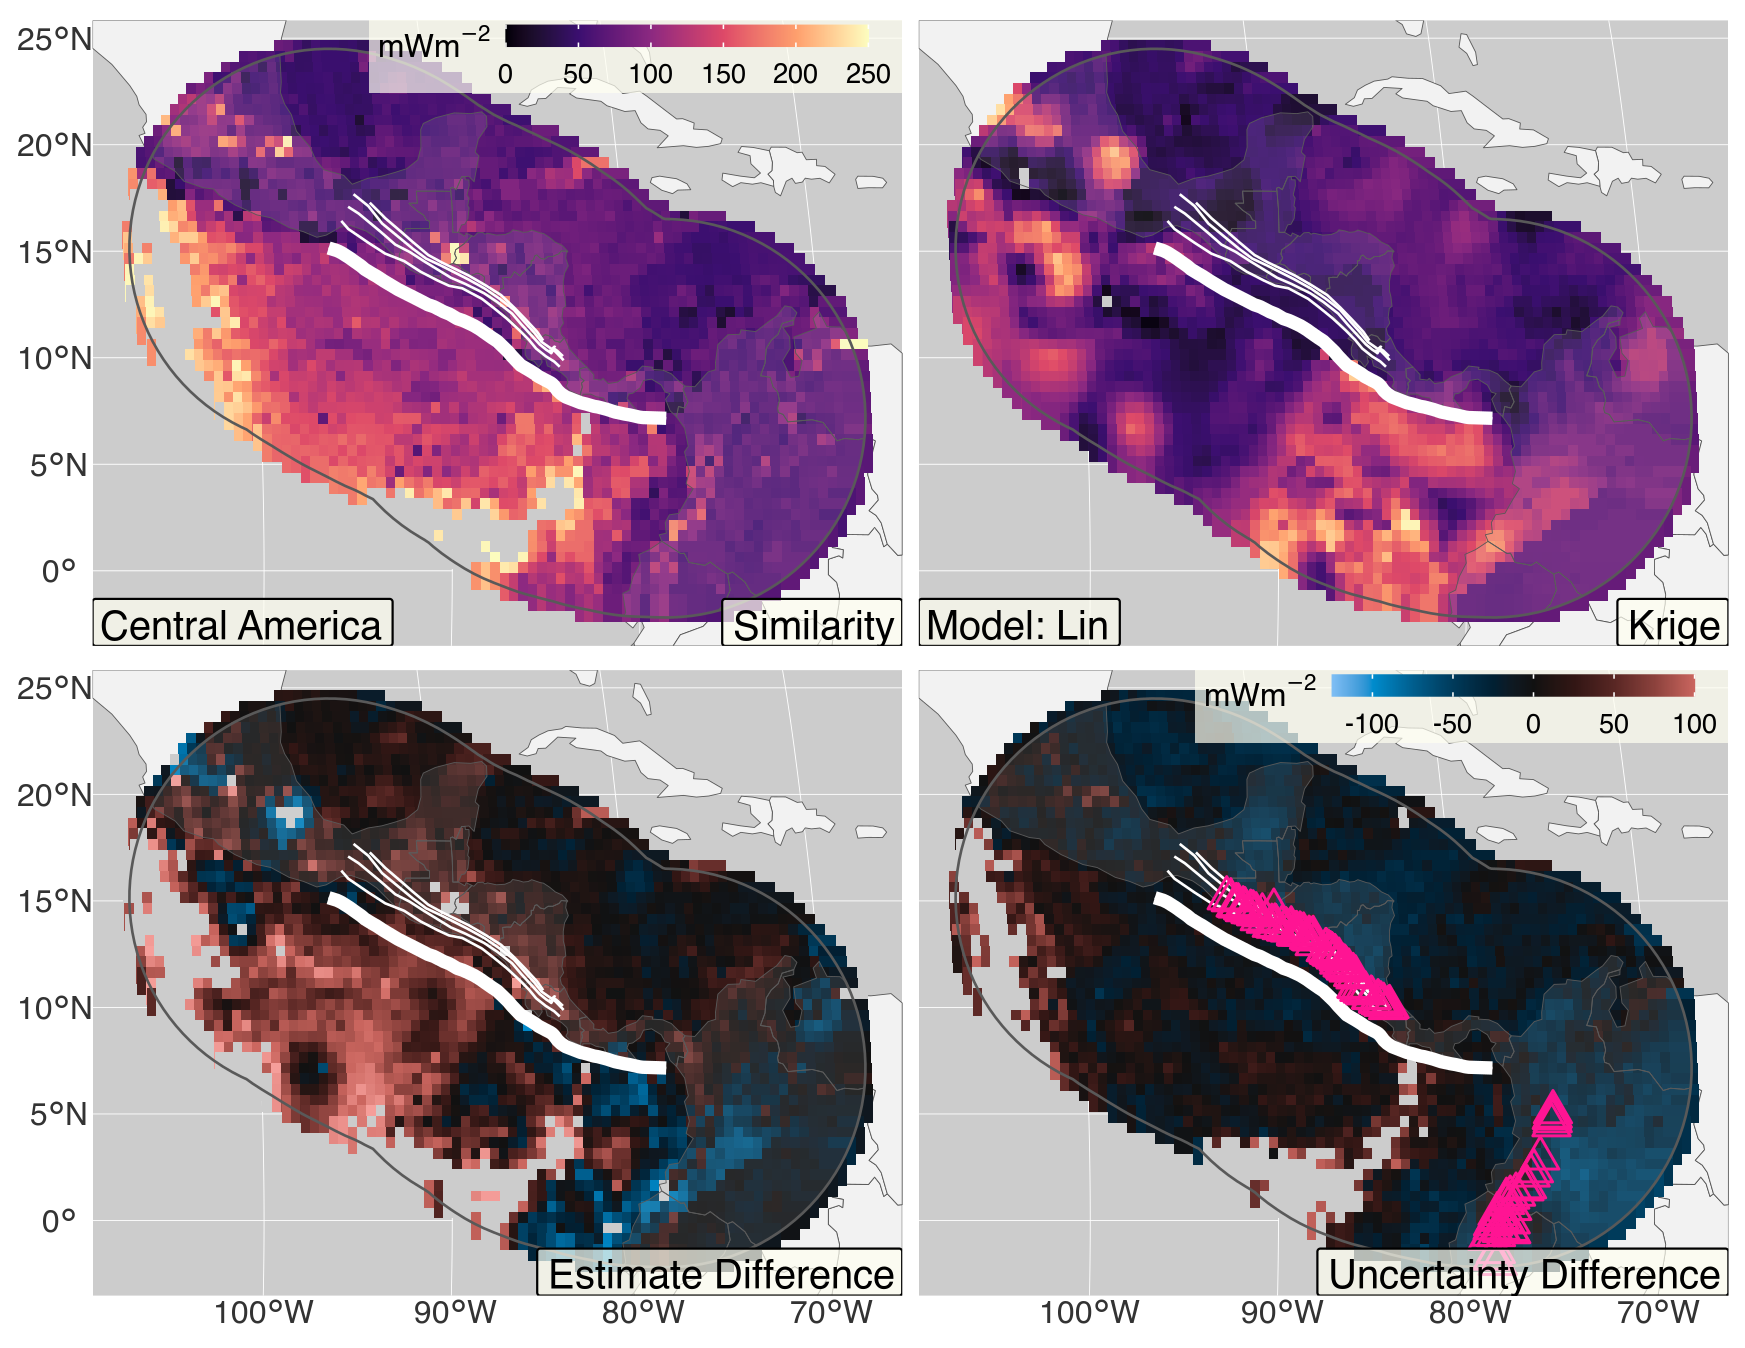
\includegraphics[width=0.67\linewidth,]{assets/figs/chpt3/CentralAmericaDiffComp} 

}

\caption[Similarity and Kriging interpolations for Central America]{Similarity and Kriging interpolations for Central America. Arms of the Galápagos triple junction (GTJ), the East Pacific Rise (EPR), and Cocos Ridge (CR), are predicted by Similarity (a), but smoothed-out by Kriging (b). Note the differences between predictions within the Cocos Plate (CP) where Similarity predicts relatively high surface heat flow compared to Kriging. Segment boundary (bold white line) and volcanoes (gold diamonds) defined by Syracuse \& Abers (\protect\hyperlink{ref-syracuse2006}{2006}). Similarity interpolation from Lucazeau (\protect\hyperlink{ref-lucazeau2019}{2019}). Plate boundaries (\DIFdelbeginFL \DIFdelFL{solid green }\DIFdelendFL \DIFaddbeginFL \DIFaddFL{bold black }\DIFaddendFL lines) defined by Lawver et al. (\protect\hyperlink{ref-lawver2018}{2018}).}\label{fig:centralAmericaDiff}
\end{figure}

\hypertarget{kyushu-ryukyu}{%
\paragraph{Kyushu Ryukyu}\label{kyushu-ryukyu}}

\DIFdelbegin \DIFdel{In contrast, Similarity and Kriging differences }\DIFdelend \DIFaddbegin \DIFadd{Similarity predicts a very textured distribution of surface heat flow throughout the Kyushu Ryukyu domain (Figure \ref{fig:kyushuRyukyuDiff}). The Similarity interpolation is clearly influenced by the locations of multiple volcanic arc chains, plate boundaries, and the age of the subducting oceanic lithosphere. The Kriging interpolation corroborates much of the texture predicted by Similarity to the NE and near the main Kyushu Ryukyu segment boundary. However, Kriging presents a smoothed-out distribution of surface heat flow within the subducting oceanic plate to the south and other large regions behind the volcanic arc chains to the west.
}

\DIFadd{Textural differences notwithstanding, regional Similarity and Kriging differences }\DIFaddend are small and narrowly distributed near Kyushu Ryukyu (median difference: 4, IQR: 22 \(mWm^{-2}\)) compared to Central America (median difference: 12, IQR: 47 \(mWm^{-2}\)\DIFaddbegin \DIFadd{; Table \ref{tab:diffSummaryTable}}\DIFaddend ). Kyushyu Ryukyu has a comparable number of observations (n = 1,895) as Central America (n = 1,443), but a simpler \DIFdelbegin \DIFdel{tectonic }\DIFdelend \DIFaddbegin \DIFadd{plate }\DIFaddend configuration (no spreading centers) and more regularly spaced observations. \DIFdelbegin \DIFdel{Kriging near Kyushu Ryukyu corroborates much of the texture predicted in the Similarity interpolation (Figure \ref{fig:kyushuRyukyuDiff}). A combination of }\DIFdelend \DIFaddbegin \DIFadd{Kyushu Ryukyu characterizes an interpolation domain with a combination of relatively }\DIFaddend high observation density, \DIFdelbegin \DIFdel{relatively uniform distribution of measurements, and relatively simple geology cause }\DIFdelend \DIFaddbegin \DIFadd{uniform observations distribution, and simple plate configuration. These characteristics apparently produce comparable }\DIFaddend Similarity and Kriging results\DIFdelbegin \DIFdel{to converge}\DIFdelend .



\begin{figure}[htbp]

{\centering 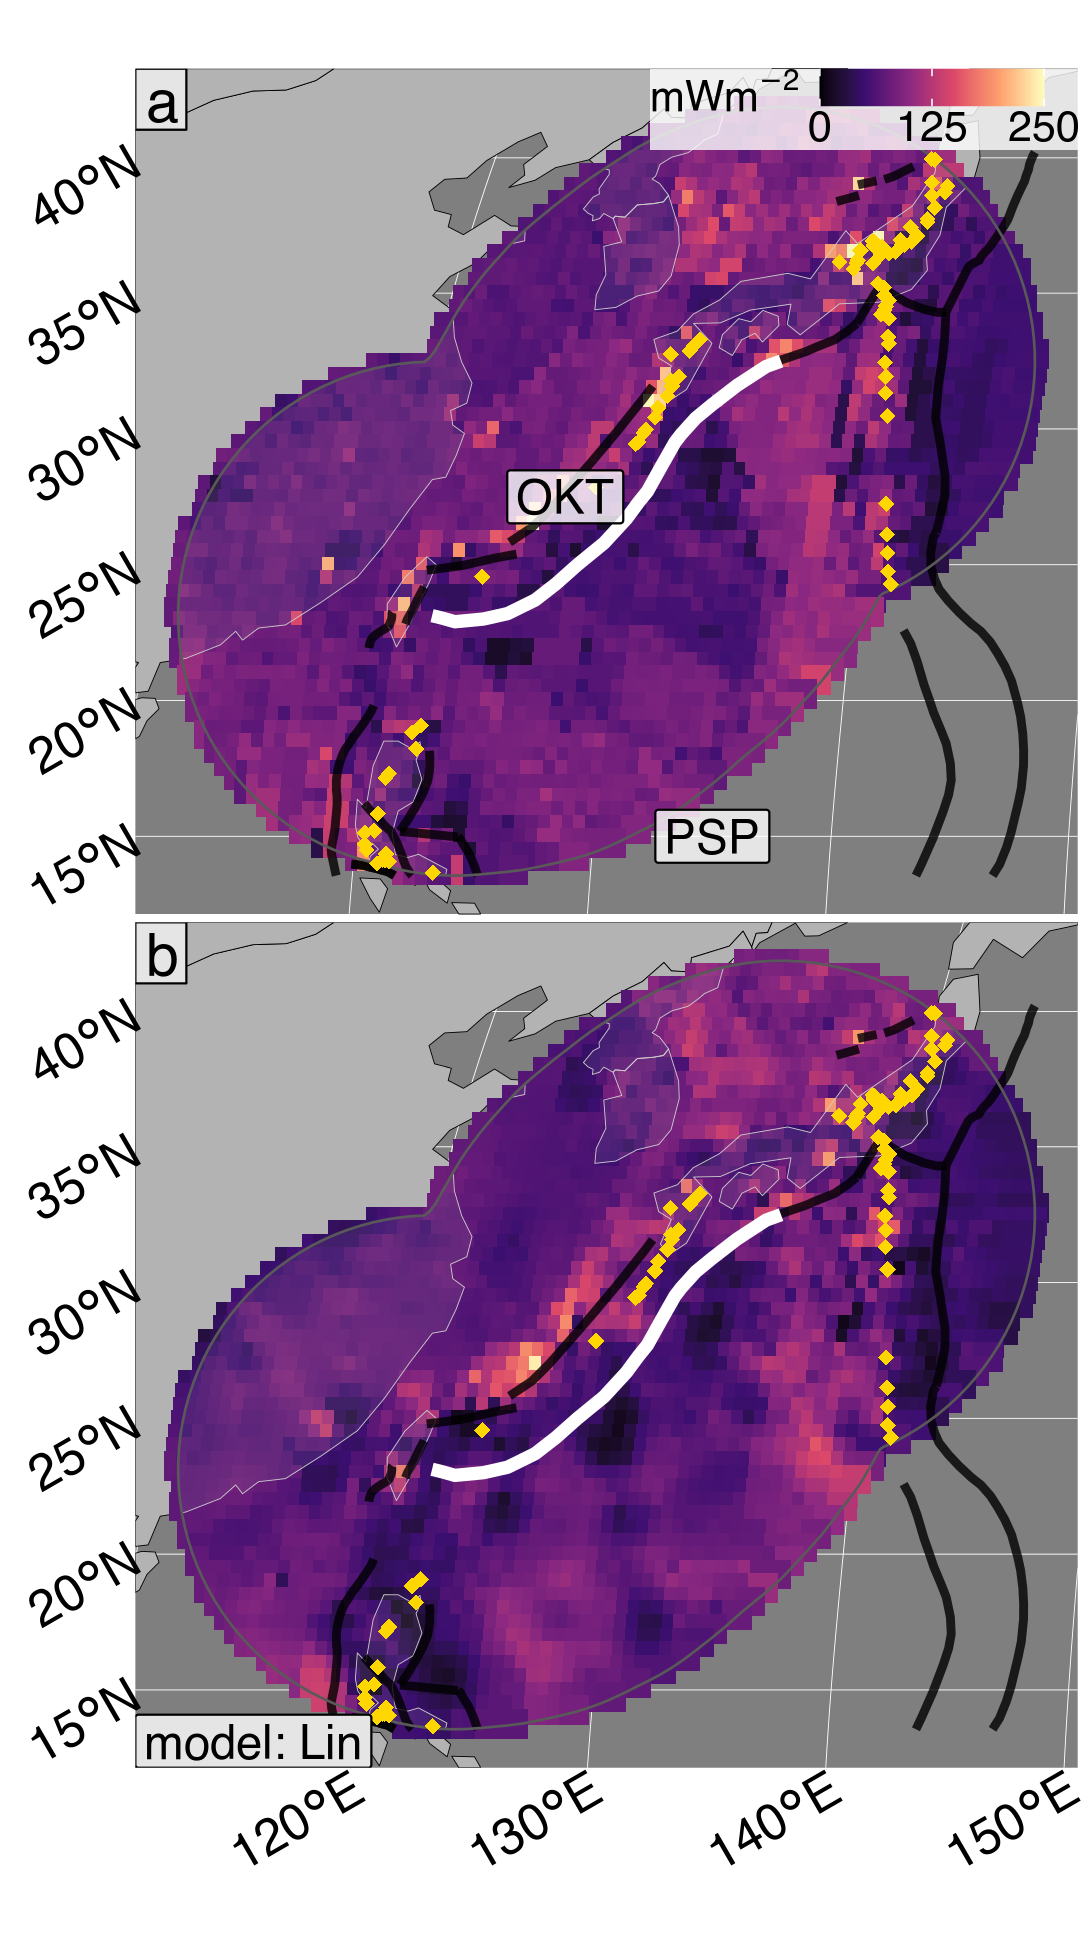
\includegraphics[width=0.63\linewidth,]{assets/figs/chpt3/KyushuRyukyuDiffComp} 

}

\caption[Similarity and Kriging interpolations for Kyushyu Ryukyu]{Similarity and Kriging interpolations for Kyushyu Ryukyu. (a) Similarity predicts a textured interpolation\DIFdelbeginFL \DIFdelFL{within the tectonically complex region}\DIFdelendFL . (b) \DIFaddbeginFL \DIFaddFL{The }\DIFaddendFL Kriging interpolation is generally smoother, but corroborate much of the same texture predicted by Similarity because of relatively high observational density and regular spatial coverage near Kyushu Ryukyu. Segment boundary (bold white line) and volcanoes (gold diamonds) defined by Syracuse \& Abers (\protect\hyperlink{ref-syracuse2006}{2006}). Similarity interpolation from Lucazeau (\protect\hyperlink{ref-lucazeau2019}{2019}). Plate boundaries (\DIFdelbeginFL \DIFdelFL{solid green }\DIFdelendFL \DIFaddbeginFL \DIFaddFL{bold black }\DIFaddendFL lines) defined by Lawver et al. (\protect\hyperlink{ref-lawver2018}{2018}).}\label{fig:kyushuRyukyuDiff}
\end{figure}

\hypertarget{scotia}{%
\paragraph{Scotia}\label{scotia}}

The Scotia segment illustrates a case where surface heat flow observations are incredibly sparse. Similarity \DIFdelbegin \DIFdel{resolves }\DIFdelend \DIFaddbegin \DIFadd{is agnostic to observational density, so it predicts multiple tectonic features including }\DIFaddend the East Scotia Ridge and the WSW-ENE trending transform boundary separating the Scotia and Sandwich Plates from the Antarctic Plate (Figure \ref{fig:scotiaDiff}). \DIFdelbegin \DIFdel{Kriging indicates }\DIFdelend \DIFaddbegin \DIFadd{Similarity predictions distal from the plate boundaries are ostensibly dependent on oceanic plate age and other small differences in the set of geologic proxies. Kriging, on the other hand, shows }\DIFaddend a heat flow anomaly more or less in the region of the East Scotia Ridge, but does not resolve \DIFaddbegin \DIFadd{any }\DIFaddend structure in a way that is geologically useful\DIFdelbegin \DIFdel{because of }\DIFdelend \DIFaddbegin \DIFadd{. Rather, }\DIFaddend very few surface heat flow observations (n = 25) \DIFdelbegin \DIFdel{. Kriging predictions thus }\DIFdelend \DIFaddbegin \DIFadd{force Kriging predictions to }\DIFaddend approximate the expected \DIFaddbegin \DIFadd{value }\DIFaddend (mean: 79 \(mWm^{-2}\)) \DIFdelbegin \DIFdel{value for the entire }\DIFdelend \DIFaddbegin \DIFadd{for most of the }\DIFaddend domain according to Equation \eqref{eq:linEstimate}.
\DIFdelbegin \DIFdel{That is, Kriging provides no more geodynamic information than computing the arithmetic mean for surface heat flow observations within a 1000 \(km\)-radius of the Scotia segment.
}\DIFdelend 



\begin{figure}[htbp]

{\centering 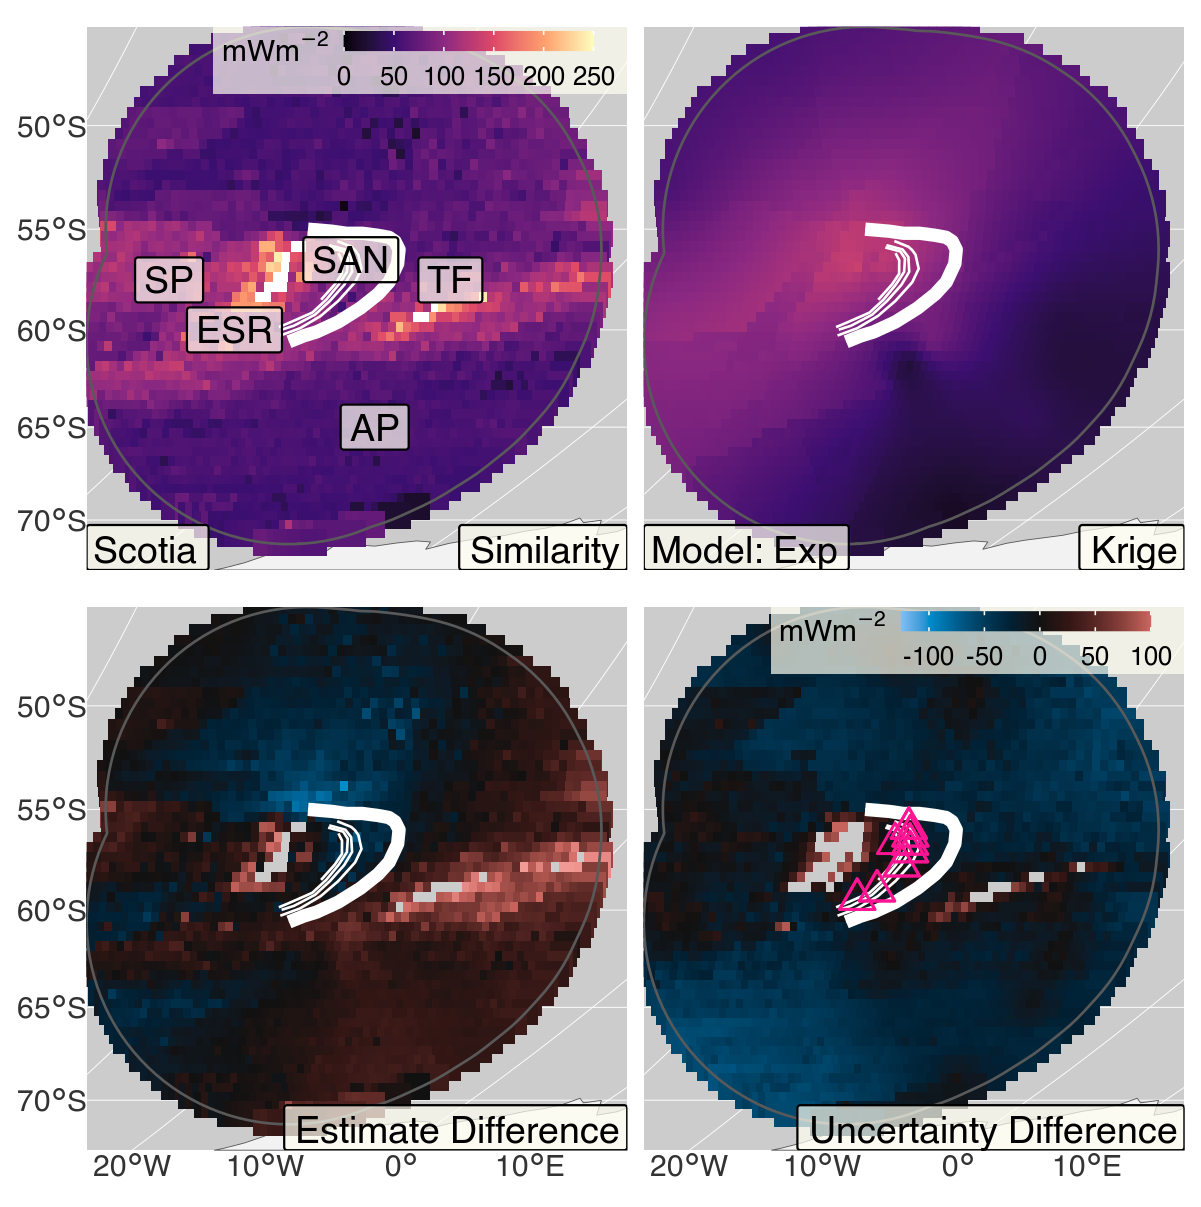
\includegraphics[width=0.56\linewidth,]{assets/figs/chpt3/ScotiaDiffComp} 

}

\caption[Similarity and Kriging interpolations for Scotia]{Similarity and Kriging interpolations for Scotia. (a) Similarity identifies two tectonic features, the East Scotia Ridge (ESR) and a transform fault (TF) separating the Scotia and Sandwich Plates (SP, SAN) from the Antartic Plate (AP). Kriging predicts a high heat flow anomaly in the region of the ESR, but otherwise appears featureless because of incredibly sparse data. Segment boundary (bold white line) and volcanoes (gold diamonds) defined by Syracuse \& Abers (\protect\hyperlink{ref-syracuse2006}{2006}). Similarity interpolation from Lucazeau (\protect\hyperlink{ref-lucazeau2019}{2019}). Plate boundaries (\DIFdelbeginFL \DIFdelFL{solid green }\DIFdelendFL \DIFaddbeginFL \DIFaddFL{bold black }\DIFaddendFL lines) defined by Lawver et al. (\protect\hyperlink{ref-lawver2018}{2018}).}\label{fig:scotiaDiff}
\end{figure}

\DIFdelbegin %DIFDELCMD < \hypertarget{upper-plate-variability}{%
%DIFDELCMD < \subsection{Upper-plate Variability}\label{upper-plate-variability}}
%DIFDELCMD < %%%
\DIFdelend \DIFaddbegin \hypertarget{upper-plate-variability}{%
\subsubsection{Upper-plate Variability}\label{upper-plate-variability}}
\DIFaddend 

\DIFdelbegin \DIFdel{Lateral surface heat flow variability across upper-plates may be categorized in 1 of 8 ways based on }\DIFdelend \DIFaddbegin \DIFadd{Sampling }\DIFaddend Similarity and Kriging \DIFdelbegin \DIFdel{prediction patterns within }\DIFdelend \DIFaddbegin \DIFadd{predictions from adjacent }\DIFaddend upper-plate sectors \DIFaddbegin \DIFadd{allows for first-order quantitative evaluation of the along-strike variability in surface heat flow. Surface heat flow distributions across sectors (defined by their medians and interquartile ranges; Table \ref{tab:sectorSummaryTable}) generally show three patterns among subduction zone segments: (1) Similarity and Kriging predictions overlap well, (2) Similarity and Kriging predictions moderately overlap, or }\DIFaddend (\DIFdelbegin \DIFdel{Table \ref{tab:lateralDiffTable}) . Each upper-plate can be characterized as having (dis) continuous Similarity prediction patterns, and /or (dis) continuous Kriging prediction patterns, }\DIFdelend \DIFaddbegin \DIFadd{3) Similarity and Kriging predictions overlap poorly. In addition to a range of overlapping Similarity }\DIFaddend and \DIFdelbegin \DIFdel{/or (in) comparable Similarity vs.~Kriging prediction patterns. Discontinuous upper-plate surface heat flow patterns are more commonly predicted by either interpolation method than continuous upper-plate surface heat flow patterns (see Appendix \ref{lateralDiffAppendix}). Discontinuous surface heat flow patterns are predicted by either Similarity or Kriging for 12/13 segments and by both Similarity and Kriging for 7/13 segments (e.g., Kyushu Ryukyu; Figure \ref{fig:kyushuRyukyuUpper}). In contrast, }\DIFdelend \DIFaddbegin \DIFadd{Kriging predictions, sector profiles show a range of bandwidths from narrow (\(\leq\) 10 \(mWm^{-2}\); }\DIFaddend continuous upper-plate surface heat flow\DIFdelbegin \DIFdel{patterns are predicted by either Similarity or Kriging for 6/13 segments and by both Similarity and Kriging for only 1/13 segments (Kamchatka Marianas; Figure \ref{fig:kamchatkaMarianasUpper}). At least 7/13 segments show incomparable }\DIFdelend \DIFaddbegin \DIFadd{) to relatively wide (up to approximately 50 \(mWm^{-2}\); discontinuous }\DIFaddend upper-plate \DIFaddbegin \DIFadd{surface heat flow). This section presents three subduction zone segments that characterize the range of observed upper-plate }\DIFaddend surface heat flow\DIFdelbegin \DIFdel{patterns predicted by Similarity and Kriging (e. g.
~Central America; Figure \ref{fig:centralAmericaUpper}).
}\DIFdelend \DIFaddbegin \DIFadd{. Visualizations of the remaining segments are presented in Appendix \ref{lateralDiffAppendix}.
}\DIFaddend 

\DIFdelbegin %DIFDELCMD < \begin{table}
%DIFDELCMD < %%%
\DIFdelendFL \DIFaddbeginFL \hypertarget{kamchatka-marianas}{%
\paragraph{Kamchatka Marianas}\label{kamchatka-marianas}}
\DIFaddendFL 



\DIFdelbeginFL %DIFDELCMD < \caption{%
{%DIFAUXCMD
%DIFDELCMD < \label{tab:lateralDiffTable}%%%
\DIFdelFL{Comparing surface heat flow patterns across upper-plate sectors}}
%DIFAUXCMD
\DIFdelendFL \DIFaddbeginFL \begin{figure}[htbp]

{\DIFaddendFL \centering \DIFdelbeginFL %DIFDELCMD < \resizebox{\linewidth}{!}{
%DIFDELCMD < \begin{tabular}[t]{llll}
%DIFDELCMD < \toprule
%DIFDELCMD < Segment & Kriging & Similarity & Comparison\\
%DIFDELCMD < \midrule
%DIFDELCMD < \cellcolor{gray!6}{Alaska Aleutians} & \cellcolor{gray!6}{discontinuous} & \cellcolor{gray!6}{discontinuous} & \cellcolor{gray!6}{comparable}\\
%DIFDELCMD < Andes & discontinuous & discontinuous & comparable\\
%DIFDELCMD < \cellcolor{gray!6}{Central America} & \cellcolor{gray!6}{discontinuous} & \cellcolor{gray!6}{discontinuous} & \cellcolor{gray!6}{incomparable}\\
%DIFDELCMD < Kamchatka Marianas & continuous & continuous & comparable\\
%DIFDELCMD < \cellcolor{gray!6}{Kyushu Ryukyu} & \cellcolor{gray!6}{discontinuous} & \cellcolor{gray!6}{discontinuous} & \cellcolor{gray!6}{comparable}\\
%DIFDELCMD < Lesser Antilles & discontinuous & discontinuous & comparable\\
%DIFDELCMD < \cellcolor{gray!6}{N Philippines} & \cellcolor{gray!6}{continuous} & \cellcolor{gray!6}{discontinuous} & \cellcolor{gray!6}{incomparable}\\
%DIFDELCMD < New Britain Solomon & continuous & discontinuous & incomparable\\
%DIFDELCMD < \cellcolor{gray!6}{S Philippines} & \cellcolor{gray!6}{discontinuous} & \cellcolor{gray!6}{discontinuous} & \cellcolor{gray!6}{incomparable}\\
%DIFDELCMD < Scotia & continuous & discontinuous & incomparable\\
%DIFDELCMD < \cellcolor{gray!6}{Sumatra Banda Sea} & \cellcolor{gray!6}{discontinuous} & \cellcolor{gray!6}{continuous} & \cellcolor{gray!6}{incomparable}\\
%DIFDELCMD < Tonga New Zealand & discontinuous & continuous & incomparable\\
%DIFDELCMD < \cellcolor{gray!6}{Vanuatu} & \cellcolor{gray!6}{discontinuous} & \cellcolor{gray!6}{discontinuous} & \cellcolor{gray!6}{comparable}\\
%DIFDELCMD < \bottomrule
%DIFDELCMD < \end{tabular}}
%DIFDELCMD < \end{table}
%DIFDELCMD < %%%
\DIFdelend \DIFaddbegin 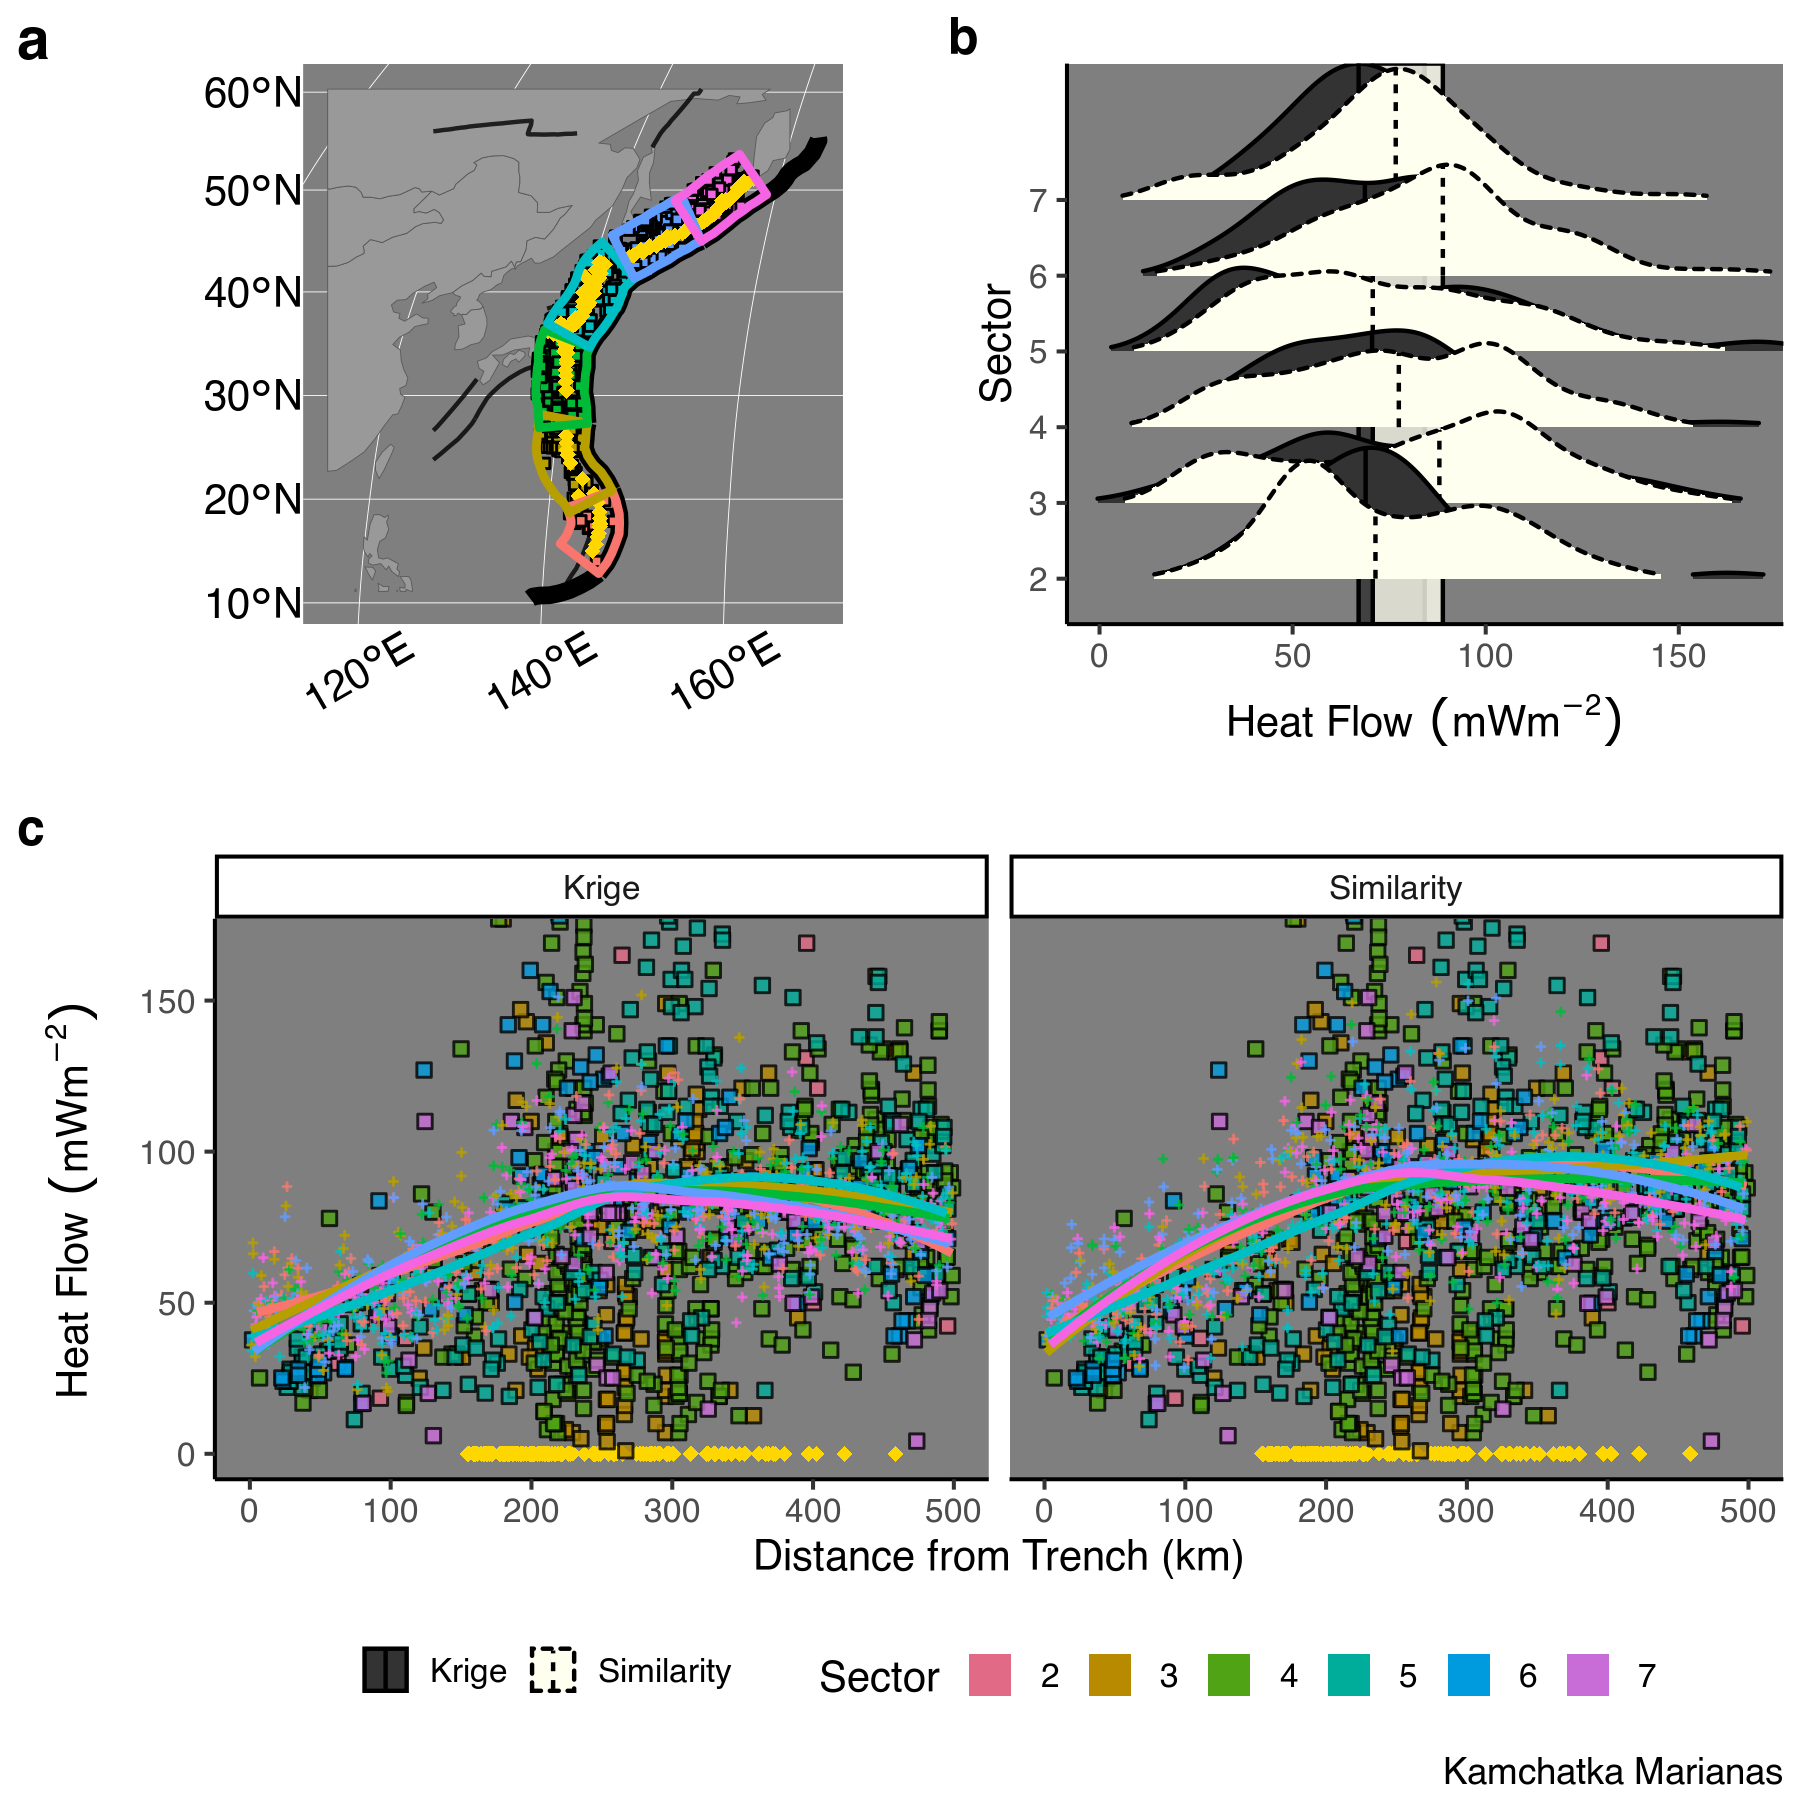
\includegraphics[width=1\linewidth,]{assets/figs/chpt3/KamchatkaMarianasUpperPlate} 
\DIFaddend 

\DIFaddbegin }

\caption[Surface heat flow profiles for Kamchatka Marianas upper-plate sectors]{\DIFadd{Surface heat flow profiles for Kamchatka Marianas upper-plate sectors. (a) Profiles are computed by finding orthogonal distances between the segment boundary (trench; bold black line) and surface heat flow predictions within eight 500 \(km\)-wide sectors (colored polygons). (b) Similarity and Kriging predictions across sectors are largely indistinguishable with overlapping interquartile ranges (boxes). (c) Profiles (colored curves with 95\% confidence intervals) are remarkably consistent across sectors for Kriging and Similarity predictions. Colored squares are ThermoGlobe data from Lucazeau (}\protect\hyperlink{ref-lucazeau2019}{2019}\DIFadd{). Segment boundary and volcanoes (gold diamonds) defined by Syracuse \& Abers (}\protect\hyperlink{ref-syracuse2006}{2006}\DIFadd{). Plate boundaries (bold black lines) defined by Lawver et al. (}\protect\hyperlink{ref-lawver2018}{2018}\DIFadd{). Profile curves in (c) are LOESS regressions through three-point running averages (small colored data points).}}\label{fig:kamchatkaMarianasUpper}
\end{figure}

\hypertarget{sumatra-banda-sea}{%
\paragraph{Sumatra Banda Sea}\label{sumatra-banda-sea}}



\DIFaddend \begin{figure}[htbp]

{\centering \DIFdelbeginFL %DIFDELCMD < 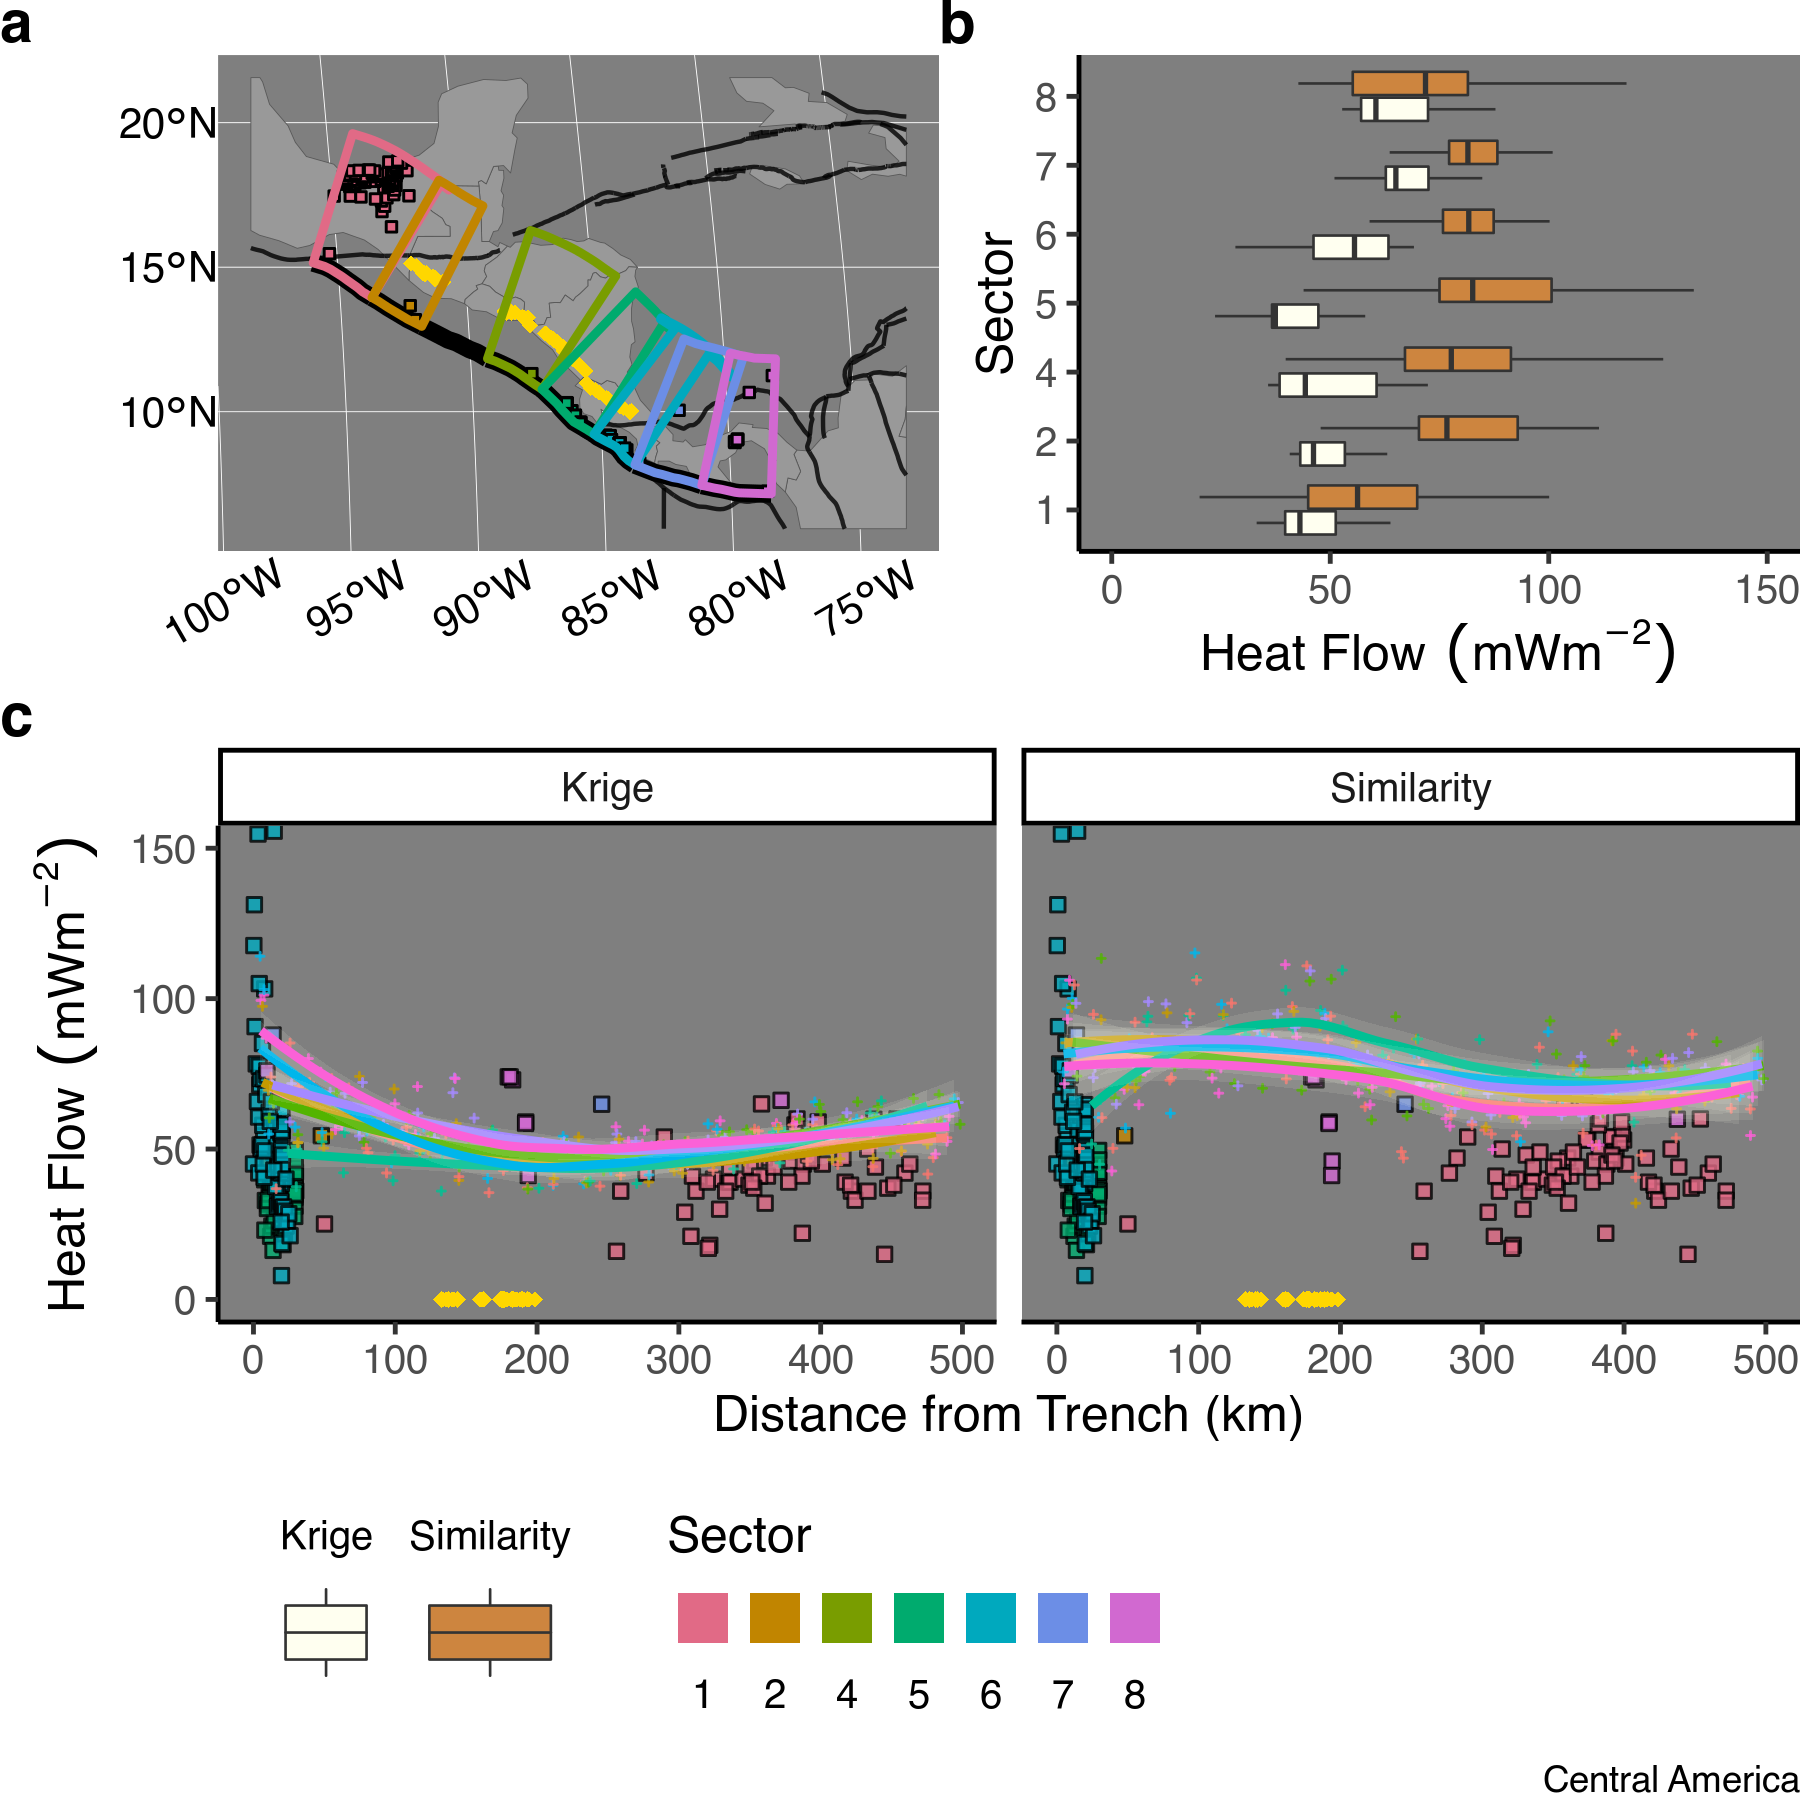
\includegraphics[width=1\linewidth,]{assets/figs/chpt3/CentralAmericaUpperPlate} 
%DIFDELCMD < %%%
\DIFdelendFL \DIFaddbeginFL 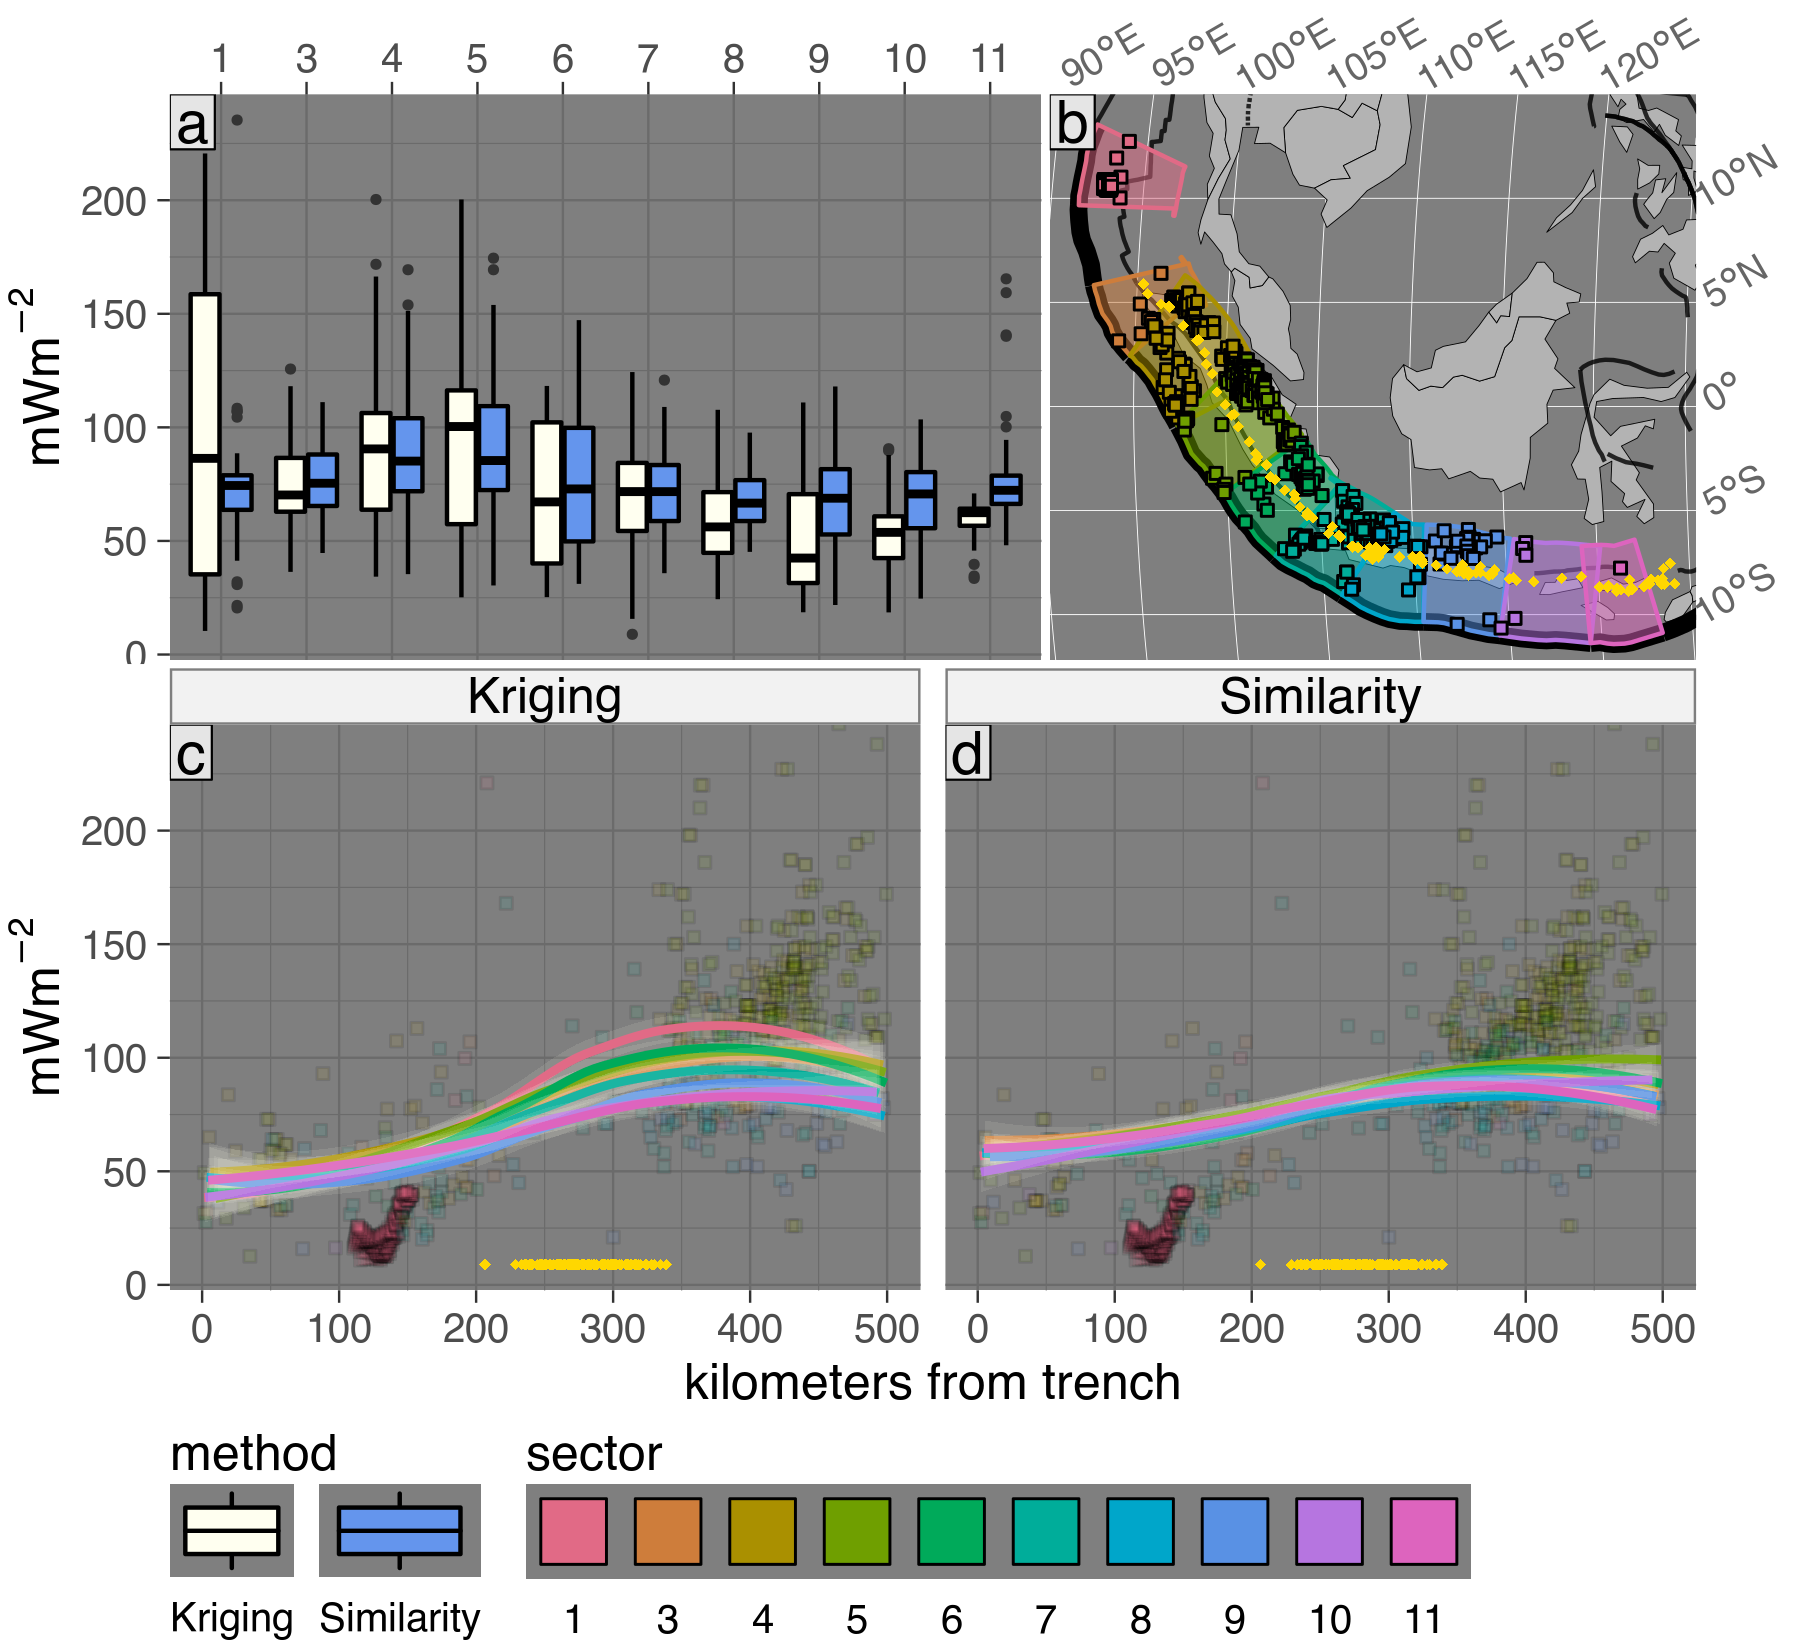
\includegraphics[width=1\linewidth,]{assets/figs/chpt3/SumatraBandaSeaUpperPlate} 
\DIFaddendFL 

}

\DIFdelbeginFL %DIFDELCMD < \caption[Along strike variability of upper-plate surface heat flow near Central America]{%%%
\DIFdelFL{Along strike variability of upper-plate surface }\DIFdelendFL \DIFaddbeginFL \caption[Surface heat flow profiles for Sumatra Banda Sea upper-plate sectors]{\DIFaddFL{Surface }\DIFaddendFL heat flow \DIFdelbeginFL \DIFdelFL{near Central America}\DIFdelendFL \DIFaddbeginFL \DIFaddFL{profiles for Sumatra Banda Sea upper-plate sectors}\DIFaddendFL . (a) \DIFdelbeginFL \DIFdelFL{Distances }\DIFdelendFL \DIFaddbeginFL \DIFaddFL{Profiles }\DIFaddendFL are computed \DIFdelbeginFL \DIFdelFL{orthogonally }\DIFdelendFL \DIFaddbeginFL \DIFaddFL{by finding orthogonal distances }\DIFaddendFL between the \DIFdelbeginFL \DIFdelFL{subduction zone }\DIFdelendFL segment boundary (\DIFaddbeginFL \DIFaddFL{trench; }\DIFaddendFL bold black line) and \DIFdelbeginFL \DIFdelFL{interpolated upper-plate }\DIFdelendFL surface heat flow \DIFdelbeginFL \DIFdelFL{targets }\DIFdelendFL \DIFaddbeginFL \DIFaddFL{predictions }\DIFaddendFL within eight 500 \(km\)-wide sectors (colored polygons). (b) Similarity \DIFdelbeginFL \DIFdelFL{predictions (dashed curves) }\DIFdelendFL and Kriging predictions \DIFdelbeginFL \DIFdelFL{(solid curves) are distinguishable }\DIFdelendFL across \DIFdelbeginFL \DIFdelFL{all }\DIFdelendFL sectors \DIFaddbeginFL \DIFaddFL{are moderately distinguishable }\DIFaddendFL with \DIFdelbeginFL \DIFdelFL{up to approximately 25 \(mWm^{-2}\) of average offset. }\DIFdelendFL \DIFaddbeginFL \DIFaddFL{mostly overlapping interquartile ranges }\DIFaddendFL (\DIFaddbeginFL \DIFaddFL{boxes), except for sectors 1 \& 6. (}\DIFaddendFL c) \DIFdelbeginFL \DIFdelFL{Both Similarity and }\DIFdelendFL \DIFaddbeginFL \DIFaddFL{Profiles (colored curves with 95\% confidence intervals) of }\DIFaddendFL Kriging predictions show \DIFdelbeginFL \DIFdelFL{discontinuous upper-plate surface heat flow with up to 25-30 \(mWm^{-2}\) differences in average upper-plate surface heat flow among sectors, but }\DIFdelendFL \DIFaddbeginFL \DIFaddFL{greater overall spread than Similarity profiles (e.g.~sector 1). Colored squares }\DIFaddendFL are \DIFdelbeginFL \DIFdelFL{distinguishable }\DIFdelendFL \DIFaddbeginFL \DIFaddFL{ThermoGlobe data }\DIFaddendFL from \DIFdelbeginFL \DIFdelFL{each other because of an average offset of approximately 25 \(mWm^{-2}\)}\DIFdelendFL \DIFaddbeginFL \DIFaddFL{Lucazeau (}\protect\hyperlink{ref-lucazeau2019}{2019}\DIFaddFL{)}\DIFaddendFL . Segment boundary \DIFaddbeginFL \DIFaddFL{and volcanoes (gold diamonds) }\DIFaddendFL defined by Syracuse \& Abers (\protect\hyperlink{ref-syracuse2006}{2006}). \DIFdelbeginFL \DIFdelFL{Curves }\DIFdelendFL \DIFaddbeginFL \DIFaddFL{Plate boundaries (bold black lines) defined by Lawver et al. (}\protect\hyperlink{ref-lawver2018}{2018}\DIFaddFL{). Profile curves }\DIFaddendFL in (c) are LOESS regressions through \DIFdelbeginFL \DIFdelFL{five-point }\DIFdelendFL \DIFaddbeginFL \DIFaddFL{three-point }\DIFaddendFL running averages \DIFaddbeginFL \DIFaddFL{(small colored data points)}\DIFaddendFL .}\DIFdelbeginFL %DIFDELCMD < \label{fig:centralAmericaUpper}
%DIFDELCMD < %%%
\DIFdelendFL \DIFaddbeginFL \label{fig:sumatraBandaSeaUpper}
\DIFaddendFL \end{figure}

\DIFaddbegin \hypertarget{new-britain-solomon}{%
\paragraph{New Britain Solomon}\label{new-britain-solomon}}



\begin{figure}[htbp]

{\centering 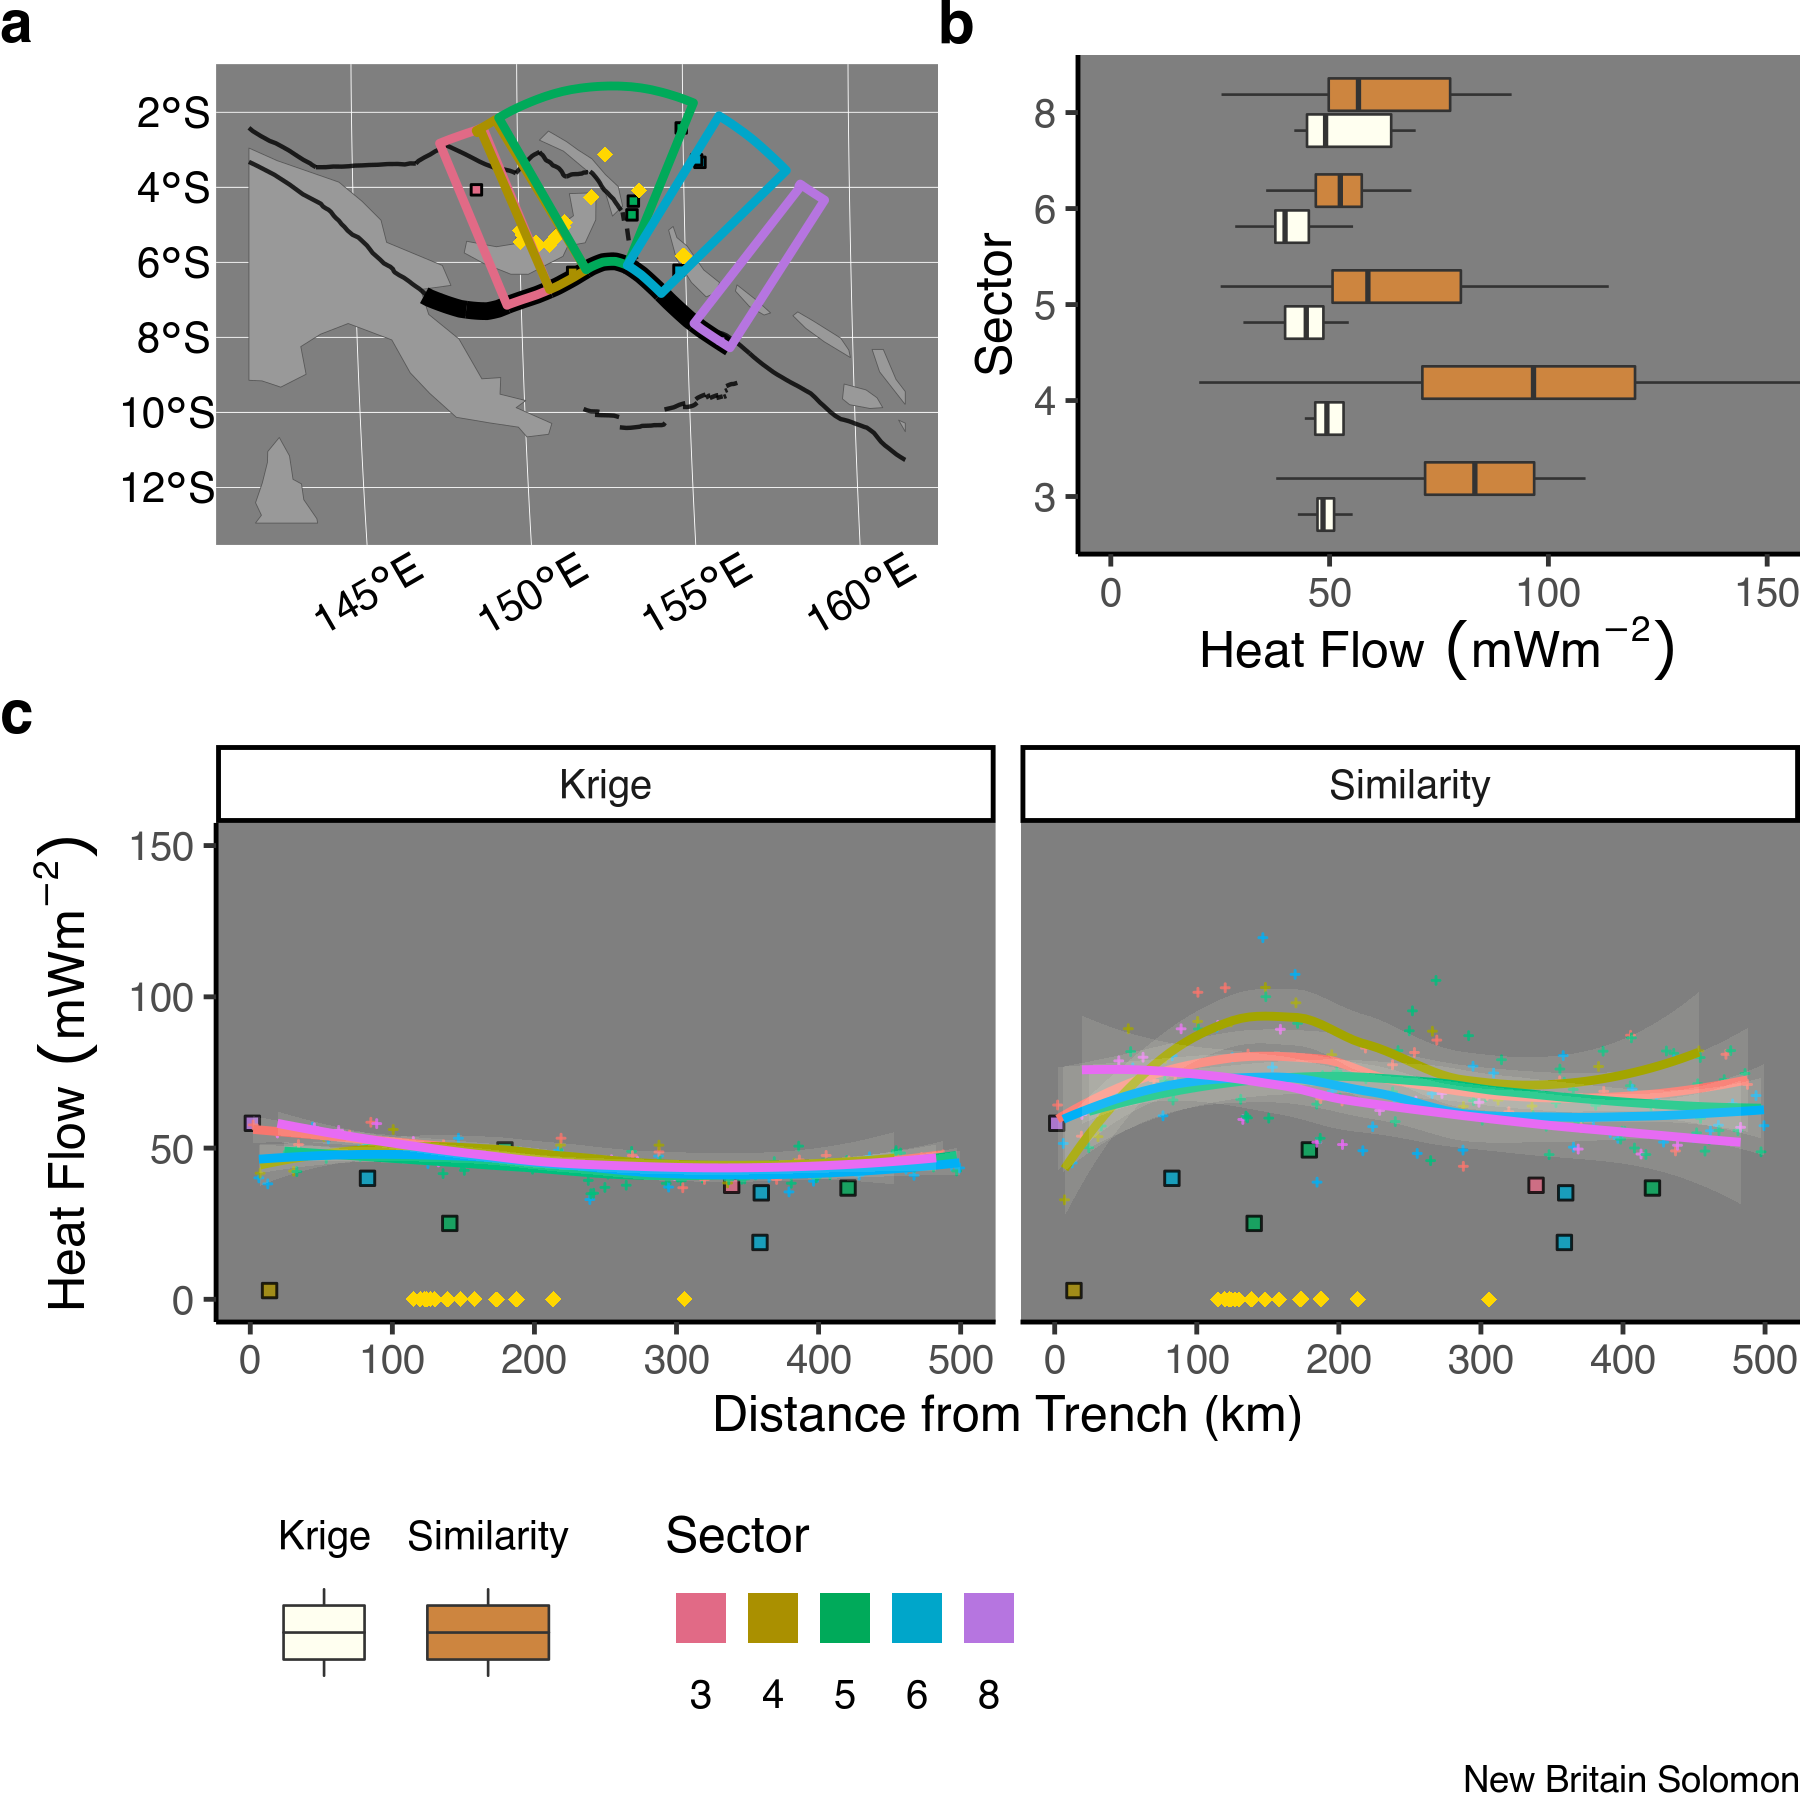
\includegraphics[width=1\linewidth,]{assets/figs/chpt3/NewBritainSolomonUpperPlate} 

}

\caption[Surface heat flow profiles for New Britain Solomon upper-plate sectors]{\DIFaddFL{Surface heat flow profiles for New Britain Solomon upper-plate sectors. (a) Profiles are computed by finding orthogonal distances between the segment boundary (trench; bold black line) and surface heat flow predictions within eight 500 \(km\)-wide sectors (colored polygons). (b) Similarity and Kriging predictions across sectors are very distinguishable with non-overlapping interquartile ranges (boxes), except for sector 8. (c) Profiles (colored curves with 95\% confidence intervals) of Kriging predictions are lower and show a smaller overall spread than Similarity profiles. Colored squares are ThermoGlobe data from Lucazeau (}\protect\hyperlink{ref-lucazeau2019}{2019}\DIFaddFL{). Segment boundary and volcanoes (gold diamonds) defined by Syracuse \& Abers (}\protect\hyperlink{ref-syracuse2006}{2006}\DIFaddFL{). Plate boundaries (bold black lines) defined by Lawver et al. (}\protect\hyperlink{ref-lawver2018}{2018}\DIFaddFL{). Profile curves in (c) are LOESS regressions through three-point running averages (small colored data points).}}\label{fig:newBritainSolomonUpper}
\end{figure}

\DIFaddend \clearpage

\hypertarget{chpt3Discussion}{%
\section{Discussion}\label{chpt3Discussion}}

\hypertarget{similarity-and-kriging-comparisons}{%
\subsection{Similarity and Kriging Comparisons}\label{similarity-and-kriging-comparisons}}

Because Similarity and Kriging are fundamentally based on different underlying mathematical frameworks, comparing surface heat flow predictions can improve understanding of subduction zone processes in the following ways.

First, comparable Similarity and Kriging interpolations can corroborate expected and/or predicted tectonic features. For example, Similarity and Kriging both predict low surface heat flow regions defining the oceanic plate and forearc along the Kamchatka Marianas segment (Figure \ref{fig:kamchatkaMarianasDiff}). Similarity and Kriging both predict high surface heat flow anomalies defining the volcanic center and transform fault separating the South American Plate and Caribbean Plates near the Lesser Antilles Segment (Figure \ref{fig:lesserAntillesDiff}). Moreover, Similarity and Kriging both predict a broad region of high surface heat flow within the NW part of the Sumatra Banda Sea segment upper-plate (Figure \ref{fig:sumatraBandaSeaDiff}), corroborating a uniformly-thin upper-plate lithosphere inferred from previous studies (\protect\hyperlink{ref-currie2006}{Currie \& Hyndman, 2006}; \protect\hyperlink{ref-hyndman2005}{Hyndman et al., 2005}). Other examples of general agreement between interpolation methods are observed near the Kyushu Ryukyu (Figure \ref{fig:kyushuRyukyuDiff}) and N Philippines segments (Figure \ref{fig:nPhilippinesDiff}). Tectonic features predicted by Similarity and Kriging are confirmed independently by prior geologic information and local surface heat flow observations.

Second, inconsistent Similarity and Kriging predictions can identify tectonic features that are unexpected or currently unresolved by either method. For example, Similarity and Kriging predictions do not confirm the same features near the Central America segment, including the location and extent of two spreading centers, the tip of a transform fault, and the thickness of the Cocos Plate (Figure \ref{fig:centralAmericaDiff}). A high heat flow anomaly defining a transform fault near the N tip of the Tonga New Zealand segment is predicted by Kriging, but not by Similarity (Figure \ref{fig:tongaNewZealandDiff}). Further, there is significant disagreement on the location of microplate boundaries predicted by Similarity vs.~Kriging near the Vanuatu segment (Figure \ref{fig:vanuatuDiff}). Features predicted by only one interpolation method either violate prior geologic information, violate local surface heat flow observations, or simply lack sufficient observational coverage to resolve by Kriging. In any case, inconsistent Similarity and Kriging predictions can identify specific features relevant targets for future data acquisition and investigation. The comparisons in Section \ref{chpt3Results} and Appendices \ref{interpDiffAppendix} \& \ref{lateralDiffAppendix} thus provide important context for subduction zone research.

\hypertarget{similarity-and-kriging-accuracies}{%
\subsection{Similarity and Kriging Accuracies}\label{similarity-and-kriging-accuracies}}

While one approach is not evidently more favorable based on first principles, regional Similarity error rates are considerably lower than Kriging (Table \ref{tab:diffSummaryTable}. However, relatively low error rates do not necessarily imply Similarity produces more accurate interpolations. It is difficult to assess the true comparative accuracy between Similarity and Kriging interpolations for two reasons. First, practically reducing Kriging error rates is possible by choosing different Kriging parameters (e.g.~the maximum number of point-pairs used for local Kriging \(n_{max}\)). While minimizing Kriging cross-validation error by an optimization procedure is a standard geostatistical approach, it does not necessarily guarantee the most accurate interpolation. For example, error rates may be reduced by highly localizing Kriging (by decreasing the number of maximum point-pairs \(n_{max}\) used for Kriging at each target location). Consequently, regional interpolation accuracy may be compromised if observations are irregularly-spaced and clustered in local high-density areas. Low Kriging error rates are therefore generally an indication of good interpolation results, but do not fully determine accuracy without evaluating the spatial relationships among observations used to calculate the error rates.

\DIFaddbegin \DIFadd{Second, Similarity's low error rates are computed with relatively few data points compared to Kriging (from Scotia: n = 25 to Lesser Antilles: n = 3010). }\DIFaddend This study computes Kriging error rates using all surface heat flow observations within the interpolation domain. In contrast, Similarity error rates are computed using a subset of observations that are explicitly co-located with the 0.5\(^\circ \times\) 0.5\(^\circ\) grid of target locations taken from Lucazeau (\protect\hyperlink{ref-lucazeau2019}{2019}). Similarity error rates may increase (or decrease) relative to Kriging error rates if computed using all observations within each interpolation domain. Computing Similarity error rates on the same set of observations as Kriging would require reproducing the Similarity results of Lucazeau (\protect\hyperlink{ref-lucazeau2019}{2019}) from the constituent proxy datasets, which are not provided as supplementary files.

Differences in error rates notwithstanding, Similarity has a distinct advantage compared to Kriging in regions with relatively low observational coverage (e.g.~Scotia; Figure \ref{fig:scotiaDiff}). While the detailed regional texture imposed by similarity is artificial insofar as it does not represent known spatial changes in surface heat flow, discrete tectonic features imposed by Similarity appear to be geodynamically consistent in most cases. Similarity may produce ostensibly accurate solutions even in cases with zero observations by integrating multiple sources of geologic information into a composite estimate of surface heat flow. This is a strength of the Similarity method that can be leveraged where limited observations preclude accurate Kriging interpolations. Regardless of methodology, the accuracy and resolution of interpolations compared in this study are sufficient to probe hypotheses about regional geodynamic uniformity among active subduction zones on the basis of surface heat flow (discussed below).

\DIFdelbegin %DIFDELCMD < \hypertarget{lateral-upper-plate-surface-heat-flow-variability}{%
%DIFDELCMD < \subsection{Lateral Upper-plate Surface Heat Flow Variability}\label{lateral-upper-plate-surface-heat-flow-variability}}
%DIFDELCMD < %%%
\DIFdelend \DIFaddbegin \hypertarget{upper-plate-sector-variability}{%
\subsection{Upper-plate Sector Variability}\label{upper-plate-sector-variability}}
\DIFaddend 

\DIFaddbegin \DIFadd{Although Kriging and Similarity predictions overlap in many sectors, differences in distributions and median predictions signal subtle but important differences in their contrasting mathematical frameworks. For example, Kriging tends to spatially smooth out surface heat flow gradients (e.g., across the trench, forearc, arc, and backarc), whereas Similarity is agnostic to gradients and can present very textured interpolations.
}

\DIFaddend Lateral variability in upper-plate surface heat flow patterns may imply spatially heterogeneous lithospheric thickness (contrary to expectations from Chapter \ref{chpt2}), spatially heterogeneous dynamics, spatially heterogeneous near-surface perturbations, and/or undersampling relative to the scale and magnitude of spatial variability. As a corollary, lateral similarity in upper-plate surface heat flow patterns imply the opposite. While uniformly thin upper-plate lithospheres and depths of plate coupling among subduction zones are inferred from similar patterns of upper-plate surface heat flow among subduction zone segments (\protect\hyperlink{ref-currie2004}{Currie et al., 2004}; \protect\hyperlink{ref-currie2006}{Currie \& Hyndman, 2006}; \protect\hyperlink{ref-furukawa1993}{Furukawa, 1993}; \protect\hyperlink{ref-kerswell2020}{Kerswell et al., 2020}; \protect\hyperlink{ref-wada2009}{Wada \& Wang, 2009}), these inferences are drawn selected transects.

In contrast, regional surface heat flow interpolations across thousands of square kilometers presented in this study clearly show very mixed results\DIFdelbegin \DIFdel{(Table \ref{tab:lateralDiffTable})}\DIFdelend . Some upper-plates appear rather uniform across large regions (e.g., Kamchatka Marianas; Figures \ref{fig:kamchatkaMarianasDiff} \& \ref{fig:kamchatkaMarianasUpper})---supporting uniformly upper-plate thickness inferred from previous work. However, many other subduction zone segments show distinct patterns of surface heat flow within several adjacent upper-plate sectors (e.g., Central America; Figures \ref{fig:centralAmericaDiff} \& \ref{fig:centralAmericaUpper}). These results stress the importance of characterizing the lateral variability of surface heat flow to better qualify claims of broad uniformity among (and within) active subduction zone segments.

\hypertarget{layered-interpolation-approach}{%
\subsection{Layered Interpolation Approach}\label{layered-interpolation-approach}}

Regional interpolation differences and distinct upper-plate surface heat flow patterns predicted by Similarity and Kriging arise from methodological differences that highlight the strengths of either method. For example, geodynamically consistent predictions are possible in regions with relatively few observations by Similarity (e.g., Scotia and New Britain Solomon; Figures \ref{fig:scotiaDiff} \& \ref{fig:newBritainSolomonDiff}), whereas resolution of unpredictable or unexpected tectonic features is possible by Kriging (e.g., Tonga New Zealand; Figure \ref{fig:tongaNewZealandDiff}). Combining the strengths of both approaches is possible using a layered interpolation approach.

For example, a Bayesian framework can be used in the following manner. First, regional Similarity is used to initialize a geodynamically consistent interpolation from geologic proxy datasets (layer 0: the priors). The prior Similarity predictions are then updated by Kriging predictions with a weighting scheme to incorporate the on-the-ground reality of surface heat flow observations. A layered approach simultaneously respects the First and Third Laws of Geography by integrating geologic and spatial information. Such an approach is generalizable to other geodynamic investigations and can be more accurate in principle, but is yet to be tried in practice (at least in the context of regional surface heat flow near subduction zone segments).

\hypertarget{conclusions-1}{%
\section{Conclusions}\label{conclusions-1}}

This study compares Kriging and Similarity interpolations to distinguish spatial patterns of surface heat flow near subduction zones. Differences between Similarity and Kriging predictions highlight at least three important points of consideration:

\begin{enumerate}
\def\labelenumi{\arabic{enumi}.}
\tightlist
\item
  In many cases Similarity and Kriging interpolations show distinct patterns of surface heat flow that highlight methodological differences between the two approaches, yet also corroborate each other in many other cases
\item
  Both Similarity and Kriging interpolations show patterns of continuous and discontinuous surface heat flow among upper-plate sectors, countering arguments of broadly uniform upper-plate thickness and plate coupling depths among (or within) subduction zone segments
\item
  Layered interpolation approaches can combine the strengths of Similarity (geodynamic consistency) and Kriging (spatial consistency) to produce more accurate surface heat flow predictions
\end{enumerate}

\cleardoublepage

\hypertarget{chpt4}{%
\chapter{Computing Rates and Distributions of Rock Recovery in Subduction Zones}\label{chpt4}}

\markboth{Chapter 4: Marker Recovery}{Chapter 4: Marker Recovery}

\DIFdelbegin %DIFDELCMD < \begin{quote}
%DIFDELCMD < %%%
\textbf{\DIFdel{Keypoints:}}
%DIFAUXCMD
%DIFDELCMD < 

%DIFDELCMD < \begin{itemize}
\begin{itemize}%DIFAUXCMD
%DIFDELCMD < \item
\item%DIFAUXCMD
%DIFDELCMD <   %%%
\DIFdel{Over one-million markers are traced across 64 subduction zone simulations
}%DIFDELCMD < \item
\item%DIFAUXCMD
%DIFDELCMD <   %%%
\DIFdel{Recovered marker }%DIFDELCMD < \gls{pt} %%%
\DIFdel{distributions are distinct from the rock record
}%DIFDELCMD < \item
\item%DIFAUXCMD
%DIFDELCMD <   %%%
\DIFdel{Marker recovery rates correlate with the thermal parameter (\(\Phi\))
}
\end{itemize}%DIFAUXCMD
%DIFDELCMD < \end{itemize}
%DIFDELCMD < \end{quote}
%DIFDELCMD < 

%DIFDELCMD < %%%
\DIFdelend \hypertarget{chpt4Abstract}{%
\section{Abstract}\label{chpt4Abstract}}

\Glsfirst{hp} metamorphic rocks that are detached (recovered) from subducting oceanic-plates and exhumed to the Earth's surface become invaluable records of P-T-strain fields deep in subduction zones. For example, comparing metamorphic \glsfirst{ptt} estimates from suites of \gls{hp} rocks allows for evaluation of \gls{pt} gradients along the plate interface through time. However, some incongruent interpretations concerning \gls{pt} gradients, recovery rates, and recovery depths arise when comparing globally aggregated \gls{ptt} estimates with \gls{pt} gradients from numerical geodynamic models. This study evaluates marker recovery in numerical simulations of oceanic-continental convergence across a range of initial thermo-kinematic boundary conditions representing presently active subduction zones. Over one-million markers traced from 64 simulated subduction zones are classified as recovered, or lost, by implementing a soft clustering classification algorithm. Marker \gls{ptt} distributions are compared across models and with the rock record to address the following questions. How do recovery rates vary among subduction zones? How is recovery distributed along the plate interface, and how does it vary among subduction zones and through time? Marker \gls{ptt} distributions and recovery rates show sensitivity to oceanic-plate age, convergence velocity, and relative detachment timing, but not to upper-plate lithospheric thickness. Marker \gls{ptt} distributions are distinct from the rock record across all but the slowest-converging (40 \(km/Ma\)) simulations. Four geodynamic regimes with different recovery modes are recognized and discussed with implications for interpreting the rock record. This study highlights the immediate usefulness of augmenting observational constraints with a large (91,733) simulated dataset.

\hypertarget{chpt4Intro}{%
\section{Introduction}\label{chpt4Intro}}

Maximum metamorphic conditions, in terms of \glsfirst{pt}, have been estimated for hundreds of \glsfirst{hp} rocks exhumed from subduction zones (Figure \ref{fig:pd15}, \protect\hyperlink{ref-agard2018}{Agard et al., 2018}; \protect\hyperlink{ref-penniston2015}{Penniston-Dorland et al., 2015}). Aggregated suites of \gls{hp} rocks (the \emph{rock record}) are the only tangible record of P-T-strain fields experienced by Earth's lithosphere during deformation and chemical processing in subduction zones (e.g., \protect\hyperlink{ref-agard2009}{Agard et al., 2009}, \protect\hyperlink{ref-agard2018}{2018}; \protect\hyperlink{ref-penniston2015}{Penniston-Dorland et al., 2015}). Together with geophysical imaging (e.g., \protect\hyperlink{ref-ferris2003}{Ferris et al., 2003}; \protect\hyperlink{ref-hyndman2003}{Hyndman \& Peacock, 2003}; \protect\hyperlink{ref-naif2015}{Naif et al., 2015}; \protect\hyperlink{ref-rondenay2008}{Rondenay et al., 2008}; \protect\hyperlink{ref-syracuse2006}{Syracuse \& Abers, 2006}), surface heat flow (e.g.~Chapter \ref{chpt3}, \protect\hyperlink{ref-currie2006}{Currie \& Hyndman, 2006}; \protect\hyperlink{ref-gao2014}{Gao \& Wang, 2014}; \protect\hyperlink{ref-hyndman2005}{Hyndman et al., 2005}; \protect\hyperlink{ref-wada2009}{Wada \& Wang, 2009}), and forward numerical modelling (e.g., \protect\hyperlink{ref-gerya2008}{Gerya et al., 2008}; \protect\hyperlink{ref-gerya2002}{Gerya et al., 2002}; \protect\hyperlink{ref-gerya2006}{Gerya \& Stöckhert, 2006}; \protect\hyperlink{ref-hacker2003}{Hacker et al., 2003}; \protect\hyperlink{ref-mckenzie1969}{McKenzie, 1969}; \protect\hyperlink{ref-peacock1990}{Peacock, 1990}, \protect\hyperlink{ref-peacock1996}{1996}; \protect\hyperlink{ref-sizova2010}{Sizova et al., 2010}; \protect\hyperlink{ref-syracuse2010}{Syracuse et al., 2010}; \protect\hyperlink{ref-yamato2007}{Yamato et al., 2007}; \protect\hyperlink{ref-yamato2008}{Yamato et al., 2008}), the rock record underpins contemporary understandings of subduction geodynamics (e.g., \protect\hyperlink{ref-agard2009}{Agard et al., 2009}, \protect\hyperlink{ref-agard2018}{2018}; \protect\hyperlink{ref-bebout2007}{Bebout, 2007}).

What geodynamic information can be extracted from the rock record? Previous work comparing \gls{pt} distributions of \gls{hp} rocks with numerical geodynamic models identifies two key observations. First, global \gls{pt} estimates compiled by Penniston-Dorland et al. (\protect\hyperlink{ref-penniston2015}{2015}) (the \texttt{pd15} dataset) reveal a kinked \gls{cdf} with respect to pressure (Figure \ref{fig:pd15}). A change in \gls{cdf} slope around 2.4 \(GPa\) implies relatively uniform recovery of oceanic material up to 2.4 \(GPa\), but increasingly rare recovery above 2.4 \(GPa\) (\protect\hyperlink{ref-agard2018}{Agard et al., 2018}; \protect\hyperlink{ref-kerswell2020}{Kerswell et al., 2020}). Note that eclogites recovered from extreme pressures above approximately 3 \(GPa\) generally have felsic compositions and typify deep subduction of continental material exhumed immediately preceding continental collision (\protect\hyperlink{ref-agard2018}{Agard et al., 2018}). While evidence of uniform mechanical coupling depths among presently active subduction zones near 2.3 \(GPa\) (\protect\hyperlink{ref-currie2006}{Currie \& Hyndman, 2006}; \protect\hyperlink{ref-furukawa1993}{Furukawa, 1993}; \protect\hyperlink{ref-kerswell2020}{Kerswell et al., 2020}; \protect\hyperlink{ref-wada2009}{Wada \& Wang, 2009}) is consistent with a relative probability decrease above 2.4 \(GPa\) implied by \texttt{pd15}'s \gls{cdf}, Chapter \ref{chpt3} shows evidence from 2D interpolations of surface heat flow in contradiction of uniform coupling depths. Moreover, it is unclear if \texttt{pd15}'s \gls{cdf} implies a shift in the probability of \emph{recovery} or \emph{exhumation} of oceanic material from around 2.4 \(GPa\), or perhaps a simpler explanation such as sampling bias (i.e.~more greenschists and blueschists have been studied relative to (ultra-)\gls{hp} rocks).

Second, \gls{hp} rocks recovered from pressures of \(\leq\) 2 \(GPa\) generally record higher temperatures than estimated by some numerical experiments (\protect\hyperlink{ref-penniston2015}{Penniston-Dorland et al., 2015}). Potential explanations for non-overlapping \gls{pt} distributions among \gls{hp} rocks and numerical models include choice of thermo-kinematic boundary conditions for numerical experiments (oceanic-plate age, convergence velocity, subduction dip angle, upper-plate thickness, heating sources, etc.), differential exhumation of \gls{hp} rocks from subduction zones with higher average \gls{pt} gradients, and comparisons among suites of undifferentiated \gls{hp} rocks with variable relative detachment timing (\protect\hyperlink{ref-abers2017}{Abers et al., 2017}; \protect\hyperlink{ref-agard2018}{Agard et al., 2018}; \protect\hyperlink{ref-kohn2018}{Kohn et al., 2018}; \protect\hyperlink{ref-penniston2015}{Penniston-Dorland et al., 2015}; \protect\hyperlink{ref-vankeken2019}{van Keken et al., 2019}). Please note, however, that many comparisons among diverse numerical experiments and metamorphic terranes show various extents of agreement depending on one's choice of initial thermo-kinematic boundary conditions and preferred suite(s) of \gls{hp} rocks (\protect\hyperlink{ref-angiboust2012b}{Angiboust et al., 2012b}; \protect\hyperlink{ref-burov2014}{Burov et al., 2014}; \protect\hyperlink{ref-holt2021}{Holt \& Condit, 2021}; \protect\hyperlink{ref-plunder2018}{Plunder et al., 2018}; \protect\hyperlink{ref-roda2010}{Roda et al., 2010}, \protect\hyperlink{ref-roda2012}{2012}, \protect\hyperlink{ref-roda2020}{2020}; \protect\hyperlink{ref-ruh2015}{Ruh et al., 2015}; \protect\hyperlink{ref-yamato2007}{Yamato et al., 2007}; \protect\hyperlink{ref-yamato2008}{Yamato et al., 2008}). Such assorted conclusions warrant further investigation into the general response of \gls{ptt} distributions to broad ranges of thermo-kinematic boundary conditions.



\begin{figure}[htbp]

{\centering 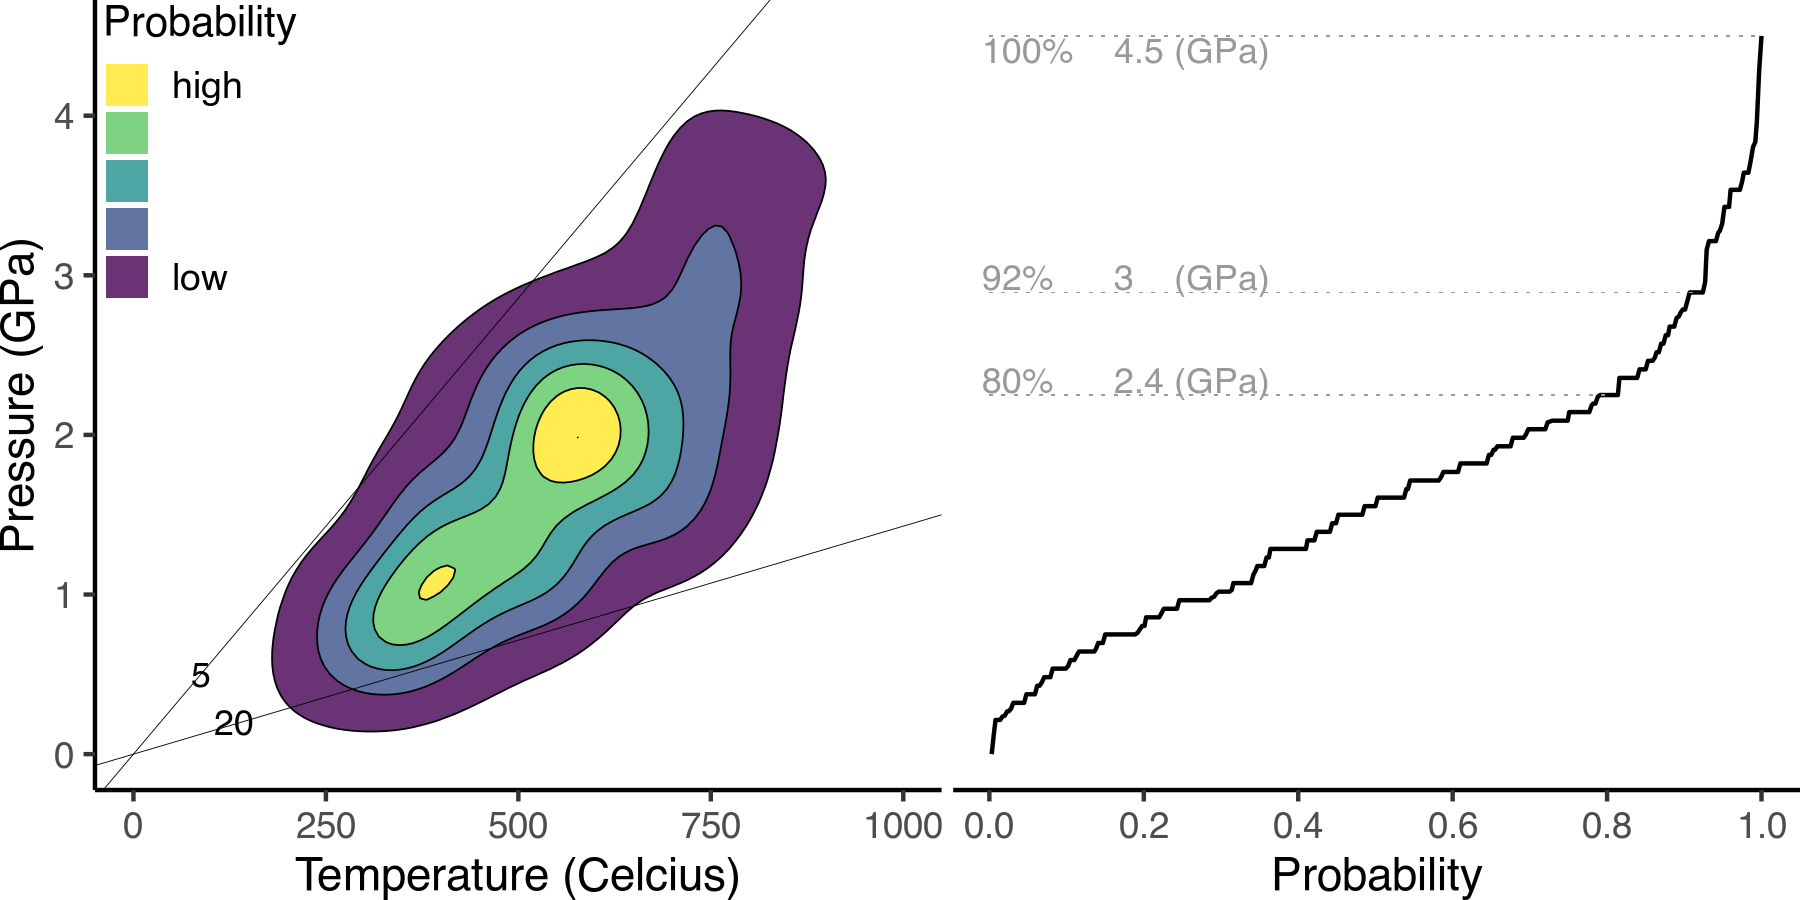
\includegraphics[width=1\linewidth,]{assets/figs/chpt4/pd15} 

}

\caption[\gls{pt} estimates from the rock record]{\gls{pt} estimates from the rock record. Maximum metamorphic conditions for exhumed \gls{hp} rocks (left; n = 354) roughly fall within thermal gradients from 5 \(K/km\) to 20 \(K/km\) (thin black lines; calculated with a lithostatic gradient of 35 \(km/GPa\)). \gls{pt} estimates are concentrated along a high-probability ridgeline that drops off sharply above 2.4 \(GPa\) (colored contours; calculated with a 2D Gaussian kernel). The \gls{cdf} (right) shows the relative probability of rock recovery explicitly with respect to pressure. Note the shared y-axis. The long ridgeline (left) and change in \gls{cdf} slope at 2.4 \(GPa\) (right) imply uniform recovery of greenschists and blueschists up to 2.4 \(GPa\), but increasingly rare eclogite recovery from depths \(\geq\) 2.4 \(GPa\). Data from Penniston-Dorland et al. (\protect\hyperlink{ref-penniston2015}{2015}).}\label{fig:pd15}
\end{figure}

Two hypotheses regarding mechanical processing of oceanic material in subduction zones follow from the above observations:

\begin{quote}
\begin{enumerate}
\def\labelenumi{\arabic{enumi}.}
\item
  The probability of recovering \gls{hp} rocks is relatively uniform up to 2.4 \(GPa\) (null: recovery is non-uniform with depth)
\item
  Recovery rates of \gls{hp} rocks vary with thermo-kinematic boundary conditions (null: recovery rates are not different among subduction zone)
\end{enumerate}
\end{quote}

These hypotheses aim at important questions in subduction zone research. Are \gls{hp} rocks recovered broadly along the plate interface or discretely? Are \gls{hp} rocks differentially recovered from subduction zones with favorable thermo-kinematic boundary conditions or is recovery ubiquitous among subduction zones? How do recovery rates change across diverse subduction zones?

The primary obstacle in addressing such questions is differentiating an unrestrained number of possible forward models with relatively few (dozens) \gls{ptt} estimates from any particular exhumed \gls{hp} metamorphic terrane. In other words, there is an imbalance between the size and scope of possible subduction zone models and the size and scope of observational constraints. This Chapter addresses the problem by augmenting observational constraints with a large (91,733) simulated \gls{ptt} dataset. More than one million markers are traced from 64 numerical experiments representing the range of thermo-kinematic boundary conditions for presently active oceanic-continental margins (experiments from Chapter \ref{chpt2}, \protect\hyperlink{ref-kerswell2020}{Kerswell et al., 2020}; \protect\hyperlink{ref-syracuse2006}{Syracuse \& Abers, 2006}; \protect\hyperlink{ref-wada2009}{Wada \& Wang, 2009}). Traced markers are classified as recovered, or lost, according to characteristics of their \gls{ptt} paths using a soft clustering classification algorithm. \gls{pt} distributions of markers appear sensitive to convergence rate and oceanic-plate age, but insensitive to upper-plate thickness (contrary to expectations from Chapter \ref{chpt2}). Further, recovery rates are strongly dependent on initial thermo-kinematic boundary conditions, characterized by the thermal parameter \(\Phi\). Four distinct geodynamic regimes are identified and their implications are discussed for interpreting aggregate \gls{pt} datasets like \texttt{pd15}.

\hypertarget{chpt4Methods}{%
\section{Methods}\label{chpt4Methods}}

This study presents a dataset of Lagrangian markers (described below) from the numerical experiments in Chapter \ref{chpt2} (\protect\hyperlink{ref-kerswell2020}{Kerswell et al., 2020}). The experiments simulate 64 oceanic-continental convergent margins with thermo-kinematic boundary conditions (oceanic-plate age, convergence velocity, and upper-plate lithospheric thickness) that generally represent the range of presently active subduction zones (\protect\hyperlink{ref-syracuse2006}{Syracuse \& Abers, 2006}; \protect\hyperlink{ref-wada2009}{Wada \& Wang, 2009}). Initial conditions were modified from previous studies of active margins (\protect\hyperlink{ref-gorczyk2007}{Gorczyk et al., 2007}; \protect\hyperlink{ref-sizova2010}{Sizova et al., 2010}). The code \texttt{I2VIS} models visco-plastic flow of geologic materials by solving three conservative equations of mass, energy, and momentum on a fully-staggered finite difference grid with a \emph{marker-in-cell} technique (\protect\hyperlink{ref-gerya2003}{Gerya \& Yuen, 2003}; \protect\hyperlink{ref-harlow1965}{Harlow \& Welch, 1965}). Further details about the initial setup, boundary conditions, and rheologic model are in Chapter \ref{chpt2} and Appendix \ref{deHydration} (\protect\hyperlink{ref-kerswell2020}{Kerswell et al., 2020}). Details about the marker-in-cell technique are in Gerya \& Yuen (\protect\hyperlink{ref-gerya2003}{2003}) and Gerya (\protect\hyperlink{ref-gerya2019}{2019}).

This section defines Lagrangian markers (now referred to as markers) and briefly elaborates on their usefulness in understanding fluid flow, followed by a description of the marker classification algorithm. Mathematical details on classification are in Appendix \ref{gmm}.

\hypertarget{lagrangian-markers}{%
\subsection{Lagrangian Markers}\label{lagrangian-markers}}

Markers are mathematical objects representing discrete parcels of fluid flowing in a continuum (\protect\hyperlink{ref-harlow1962}{Harlow, 1962}, \protect\hyperlink{ref-harlow1964}{1964}). Tracing markers (saving marker information at each timestep) is distinctly advantageous for investigating subduction dynamics in the following two ways.

First, under a set of assumptions, tracing markers is like tracing a rock's \gls{ptt} history. Assumptions in this study include an incompressible continuum (\protect\hyperlink{ref-batchelor1953}{Batchelor, 1953}; \protect\hyperlink{ref-boussinesq1897}{Boussinesq, 1897}), a petrologic model governing marker material properties (\protect\hyperlink{ref-ito1971}{Ito \& Kennedy, 1971}; \protect\hyperlink{ref-schmidt1998}{Schmidt \& Poli, 1998}), and a highly non-linear rheologic model relating stress and strain by empirical flow laws (\protect\hyperlink{ref-hilairet2007}{Hilairet et al., 2007}; \protect\hyperlink{ref-karato1993}{Karato \& Wu, 1993}; \protect\hyperlink{ref-ranalli1995}{Ranalli, 1995}; \protect\hyperlink{ref-turcotte2002}{Turcotte \& Schubert, 2002}). Insofar as Earth's lithosphere behave like an incompressible visco-plastic fluid (under the assumptions above, \protect\hyperlink{ref-gerya2019}{Gerya, 2019}; \protect\hyperlink{ref-gerya2003}{Gerya \& Yuen, 2003}; \protect\hyperlink{ref-kerswell2020}{Kerswell et al., 2020}), comparisons between marker \gls{ptt} paths and the rock record may be made.

Second, markers deform in a partly layered, partly heterogeneous, high-strain region known as the \emph{plate interface}, \emph{subduction interface}, or \emph{subduction channel} (\protect\hyperlink{ref-gerya2002}{Gerya et al., 2002}). Current conceptual models of the plate interface epitomize a visco-plastic continuum with complex geometry and structure, sharp thermal, chemical, and strain gradients, strong advection, and abundant fluid flow (\protect\hyperlink{ref-agard2016}{Agard et al., 2016}, \protect\hyperlink{ref-agard2018}{2018}; \protect\hyperlink{ref-bebout2007}{Bebout, 2007}; \protect\hyperlink{ref-bebout2002}{Bebout \& Barton, 2002}; \protect\hyperlink{ref-gerya2003}{Gerya \& Yuen, 2003}; \protect\hyperlink{ref-penniston2015}{Penniston-Dorland et al., 2015}; \protect\hyperlink{ref-syracuse2010}{Syracuse et al., 2010}). Because finite-difference numerical approaches do not perform well with strong local gradients, interpolating and updating temperature, strain, and chemical fields with markers greatly improves accuracy and stability of numerical solutions (\protect\hyperlink{ref-gerya2019}{Gerya, 2019}; \protect\hyperlink{ref-gerya2003}{Gerya \& Yuen, 2003}; \protect\hyperlink{ref-moresi2003}{Moresi et al., 2003}).

\hypertarget{marker-classification}{%
\subsection{Marker Classification}\label{marker-classification}}

On average, 18,981 markers are initially selected from within a 760 \(km\) wide and 8 \(km\) deep section of oceanic crust and seafloor sediments at \(t\) = 0 \(Ma\). Tracing proceeds for 79 timesteps, which is sufficient for most markers to be deeply subducted (\(\geq\) 200 \(km\)) from their initial positions. However, only markers recovered from the subducting oceanic-plate are relevant for comparison with \gls{pt} estimates of natural rocks. The main challenge, therefore, is to first determine which markers among 1,214,757 detach and move away from the subducting plate without knowing their fate \emph{a priori}.

Classifying markers as either \emph{recovered} or \emph{lost} based solely on their undifferentiated traced histories defines an unsupervised classification problem (\protect\hyperlink{ref-barlow1989}{Barlow, 1989}). This study implements a Gaussian mixture model (Appendix \ref{gmm}, \protect\hyperlink{ref-reynolds2009}{Reynolds, 2009}), which is a type of ``soft'' clustering algorithm used extensively to solve such problems. In this case, Gaussian mixture model organizes markers into groups (clusters) by fitting \(k=10\) bivariate Gaussian distributions to their maximum \gls{pt} (attained at depths of at least 20 \(km\); maximum P and T are considered independently). ``Fitting'' refers to adjusting parameters of all \(k\) Gaussians (centroids and covariance matrices) until the Gaussian ellipsoids and data achieve maximum likelihood (see Appendix \ref{gmm}). Groups of markers are then labeled as either \emph{recovered} or \emph{lost} based on cluster centroid locations in \gls{pt} space and other simple rules given in Table \ref{tab:rules}.

\DIFaddbegin \begin{landscape}\DIFaddend \begin{table}

\caption{\label{tab:rules}Classifier rules and total class counts}
\centering
\DIFdelbeginFL %DIFDELCMD < \resizebox{\linewidth}{!}{
%DIFDELCMD < \begin{threeparttable}
%DIFDELCMD < \begin{tabular}[t]{rlll}
%DIFDELCMD < \toprule
%DIFDELCMD < Rule & Explanation & Class & Total\\
%DIFDELCMD < \midrule
%DIFDELCMD < \cellcolor{gray!6}{1} & \cellcolor{gray!6}{max P is reached after collision with convergence region} & \cellcolor{gray!6}{collision (lost)} & \cellcolor{gray!6}{188,603}\\
%DIFDELCMD < 2 & marker changes into melt or water & phase change (lost) & 101,191\\
%DIFDELCMD < \cellcolor{gray!6}{3} & \cellcolor{gray!6}{T never exceeds 50 $^\circ$C} & \cellcolor{gray!6}{T anomaly (lost)} & \cellcolor{gray!6}{4,176}\\
%DIFDELCMD < 4 & extreme non-lithostatic max P & P anomaly (lost) & 17,504\\
%DIFDELCMD < \cellcolor{gray!6}{5} & \cellcolor{gray!6}{max P is 7.5$\sigma$ above the mean (recovered) max P} & \cellcolor{gray!6}{P anomaly (lost)} & \cellcolor{gray!6}{90}\\
%DIFDELCMD < 6 & cluster centroid is below a $5\ K/km$ gradient & subducted (lost) & 815,605\\
%DIFDELCMD < \cellcolor{gray!6}{7} & \cellcolor{gray!6}{none of the above} & \cellcolor{gray!6}{recovered} & \cellcolor{gray!6}{91,733}\\
%DIFDELCMD < \bottomrule
%DIFDELCMD < \end{tabular}
%DIFDELCMD < \begin{tablenotes}
%DIFDELCMD < \item \uline{\textit{Rule 1}}: refers to collision between trench sediments and a rectangular convergence region centered at 500 $km$ from the left boundary. Marker \gls{pt} paths after collision are unrepresentative of natural buoyancy-driven plate motions.
%DIFDELCMD < \item \uline{\textit{Rule 4}}: refers to markers that experience extreme deviatoric stress and thus have max P's that do not correspond to max depth.
%DIFDELCMD < \end{tablenotes}
%DIFDELCMD < \end{threeparttable}}
%DIFDELCMD < %%%
\DIFdelendFL \DIFaddbeginFL \begin{threeparttable}
\begin{tabular}[t]{rlll}
\toprule
\DIFaddFL{Rule }& \DIFaddFL{Explanation }& \DIFaddFL{Class }& \DIFaddFL{Total}\\
\midrule
\cellcolor{gray!6}{1} & \cellcolor{gray!6}{max P is reached after collision with convergence region} & \cellcolor{gray!6}{collision (lost)} & \cellcolor{gray!6}{188,603}\\
\DIFaddFL{2 }& \DIFaddFL{marker changes into melt or water }& \DIFaddFL{phase change (lost) }& \DIFaddFL{101,191}\\
\cellcolor{gray!6}{3} & \cellcolor{gray!6}{T never exceeds 50 $^\circ$C} & \cellcolor{gray!6}{T anomaly (lost)} & \cellcolor{gray!6}{4,176}\\
\DIFaddFL{4 }& \DIFaddFL{extreme non-lithostatic max P }& \DIFaddFL{P anomaly (lost) }& \DIFaddFL{17,504}\\
\cellcolor{gray!6}{5} & \cellcolor{gray!6}{max P is 7.5$\sigma$ above the mean (recovered) max P} & \cellcolor{gray!6}{P anomaly (lost)} & \cellcolor{gray!6}{90}\\
\DIFaddFL{6 }& \DIFaddFL{cluster centroid is below a $5\ K/km$ gradient }& \DIFaddFL{subducted (lost) }& \DIFaddFL{815,605}\\
\cellcolor{gray!6}{7} & \cellcolor{gray!6}{none of the above} & \cellcolor{gray!6}{recovered} & \cellcolor{gray!6}{91,733}\\
\bottomrule
\end{tabular}
\begin{tablenotes}
\item \uline{\textit{Rule 1}}\DIFaddFL{: refers to collision between trench sediments and a rectangular convergence region centered at 500 $km$ from the left boundary. Marker }\gls{pt} \DIFaddFL{paths after collision are unrepresentative of natural buoyancy-driven plate motions.
}\item \uline{\textit{Rule 4}}\DIFaddFL{: refers to markers that experience extreme deviatoric stress and thus have max P's that do not correspond to max depth.
}\end{tablenotes}
\end{threeparttable}
\DIFaddendFL \end{table}
\DIFaddbegin \end{landscape}
\DIFaddend 



\begin{figure}[htbp]

{\centering 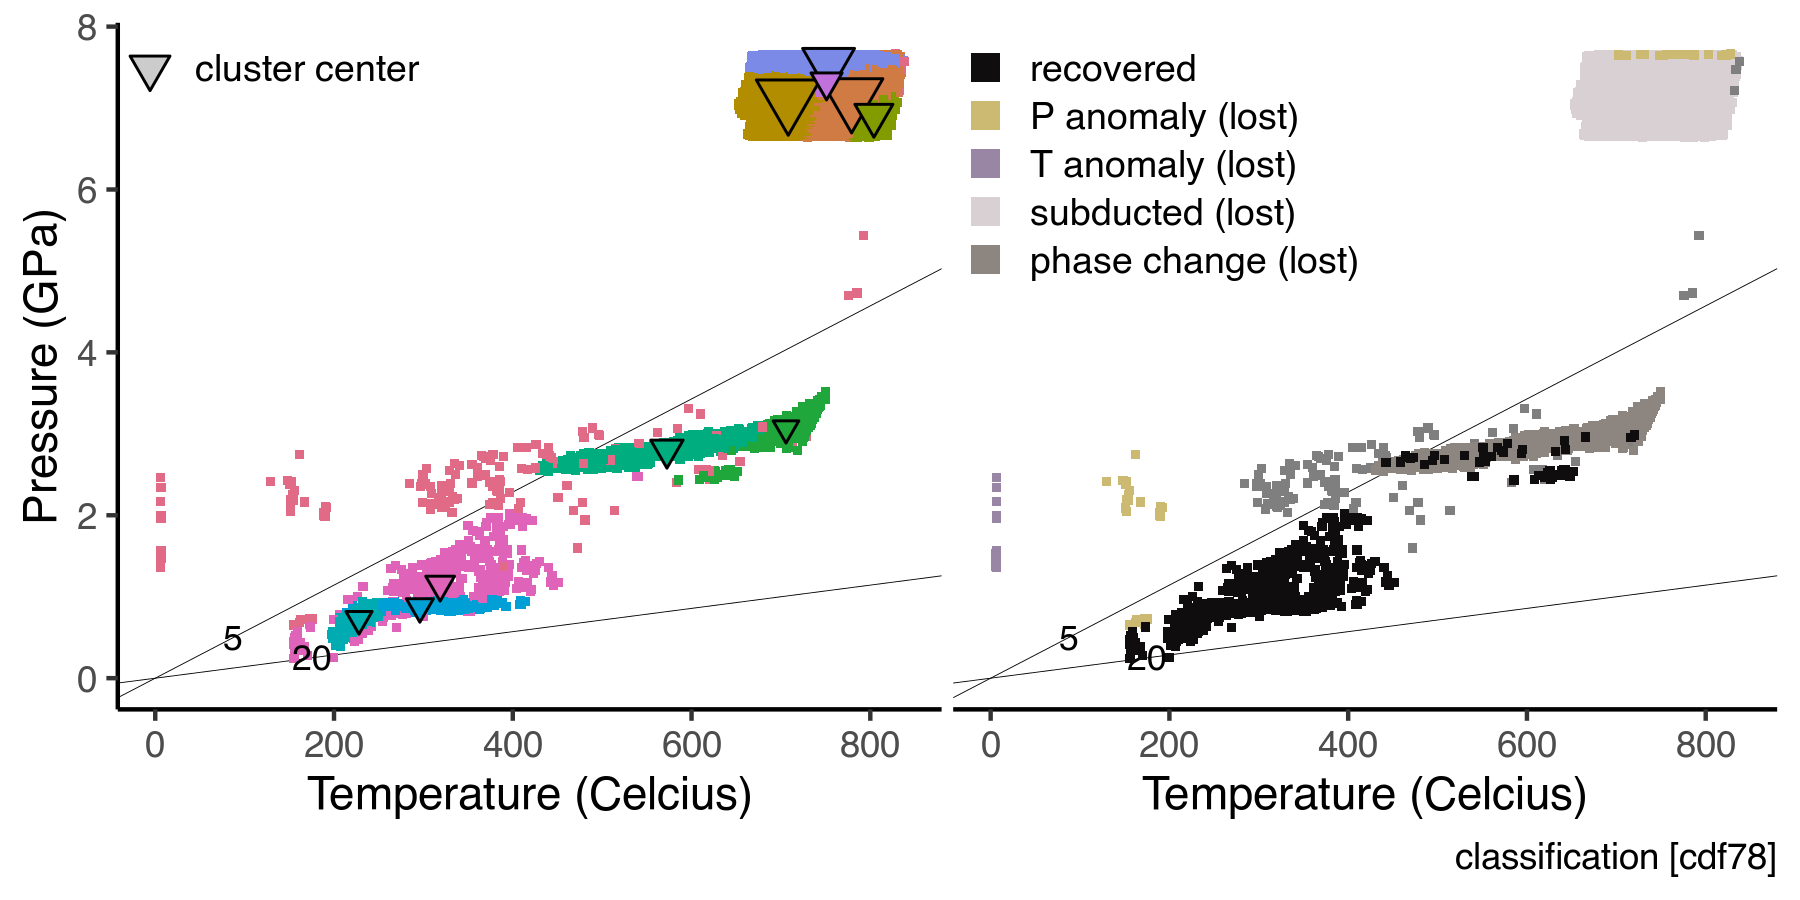
\includegraphics[width=1\linewidth,]{assets/figs/chpt4/k10/cdf78_class} 

}

\caption[Example of marker classification for model cdf78]{Example of marker classification for model cdf78. Clustering assigns 18,934 markers (squares) into ten classes according to their maximum \gls{pt} relative to all other markers (left). The size of cluster centroids (triangles) are proportional to the number of markers in a class. Markers belonging to clusters with centroids that have average \gls{pt} gradients greater than 5 \(K/km\) (plotting to the right of the thin black line labelled ``5'') classify as recovered. Additional rules are applied to (re)classify individual markers (right; see Table \ref{tab:rules}). Thin black lines are average \gls{pt} gradients of 5 \(K/km\) and 20 \(K/km\) (calculated with a lithostatic gradient of 35 \(km/GPa\)).}\label{fig:class}
\end{figure}

Please note that classification is possible by directly applying simple rules without clustering (e.g.~markers reach a max depth of \(Z\) before returning to a depth of \(Z-dZ\), \protect\hyperlink{ref-roda2010}{Roda et al., 2010}). This is an example of ``hard'' classification that assigns binary labels (marker is either recovered or lost), which is generally less flexible than ``soft'' approaches like Gaussian mixture model that assign probabilities (maker is 85\% likely recovered, 15\% likely lost). Similar approaches using Gaussian mixture model are broadly used in many scientific fields for pattern recognition, anomaly detection, and estimating complex probability distribution functions (e.g., \protect\hyperlink{ref-banfield1993}{Banfield \& Raftery, 1993}; \protect\hyperlink{ref-celeux1995}{Celeux \& Govaert, 1995}; \protect\hyperlink{ref-figueiredo2002}{Figueiredo \& Jain, 2002}; \protect\hyperlink{ref-fraley2002}{Fraley \& Raftery, 2002}; \protect\hyperlink{ref-vermeesch2018}{Vermeesch, 2018}). Moreover, clustering methods (Appendix \ref{gmm}) may be generally adopted to distinguish many possible feature(s) in geodynamic numerical models with Lagrangian reference frames. Figure \ref{fig:class} shows an example of marker classification for 1 of 64 numerical experiments. All other experiments are in Appendix \ref{vis}.

\hypertarget{chpt4Results}{%
\section{Results}\label{chpt4Results}}

\hypertarget{pt-distributions-of-recovered-markers}{%
\subsection{PT Distributions of Recovered Markers}\label{pt-distributions-of-recovered-markers}}

Markers compiled from all numerical experiments show distinct patterns of probability density and absolute \gls{pt} compared to \texttt{pd15} (Figure \ref{fig:meta}). Marker density is asymmetric and bimodal with a high-probability peak around 1 \(GPa\) (lower-blueschist to upper-greenschist facies) and a modest probability hill aroung 2.5 \(GPa\) (upper-blueschist to eclogite facies). The probability density distribution of \texttt{pd15}, in contrast, is slightly shifted towards higher \gls{pt} gradients overall and is more uniformly distributed along a high-probability ridgeline spanning from 0.8 to 2.4 \(GPa\) (upper-greenschist to lower-eclogite facies). \gls{hp} rocks recovered from 0.8 \(GPa\) to 2.4 \(GPa\) are especially overrepresented in \texttt{pd15} compared to markers compiled from all numerical experiments (Figure \ref{fig:meta}).



\begin{figure}[htbp]

{\centering 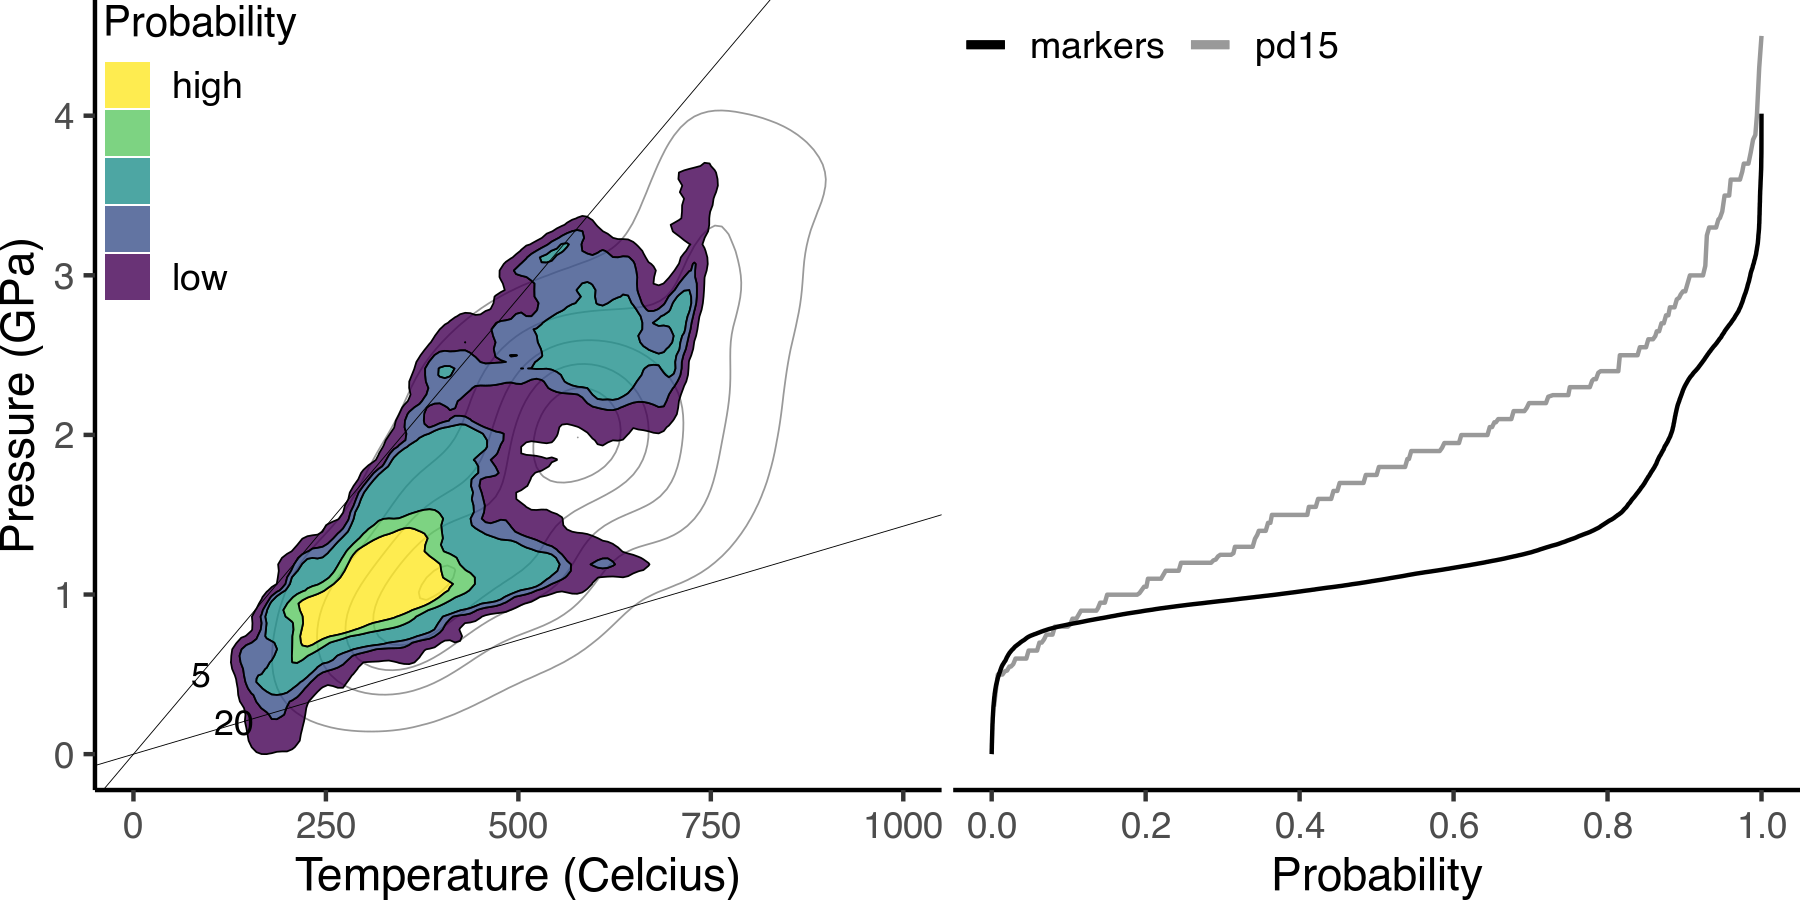
\includegraphics[width=1\linewidth,]{assets/figs/chpt4/meta} 

}

\caption[\gls{pt} distribution of recovered markers from all simulations]{\gls{pt} distribution of recovered markers from all simulations. Maximum \gls{pt} for 91,733 recovered markers compiled from all 64 subduction zone simulations (left; colored contours) show an asymmetric, bimodal distribution with a high-probability peak around 1 \(GPa\) (upper-greenschist to lower-blueschist facies) and a modest probability hill around 2.5 \(GPa\) (upper-blueschist to eclogite facies). Recovered markers neither completely overlap with the rock record (\texttt{pd15}; light gray density contours) in absolute \gls{pt} nor in terms of probability density. The \gls{cdf} (right) shows markers recovered between approximately 0.8 and 2.4 \(GPa\) (greenschists to upper-blueschist) are especially overrepresented in the rock record (\texttt{pd15}; gray line) compared to simulations (black line). Rocks with maximum pressures above 2.4 \(GPa\) (eclogites) are also overrepresented in the rock record (to a lesser degree) compared to simulations. Note that the gap between the gray and black lines (right) represents the relative difference in abundance of recovered material between \texttt{pd15} and simulations. Thin black lines are average \gls{pt} gradients of 5 \(K/km\) and 20 \(K/km\) (calculated with a lithostatic gradient of 35 \(km/GPa\)).}\label{fig:meta}
\end{figure}

To better understand how rock recovery varies among subduction zones, marker \gls{pt} distributions are visualized in terms of convergence velocity (Figure \ref{fig:cvDensity}), oceanic-plate age (Figure \ref{fig:ageDensity}), upper-plate lithospheric thickness (Figure \ref{fig:zupDensity}), and relative detachment timing (Figure \ref{fig:detachDensity}). Each of these effects is summarised below.

\begingroup
\DIFdelbegin %DIFDELCMD < \renewcommand{\baselinestretch}{1.25}
%DIFDELCMD < %%%
\DIFdelend \DIFaddbegin \renewcommand{\arraystretch}{0.5}
\DIFaddend 

\begin{landscape}\begingroup\DIFdelbegin %DIFDELCMD < \fontsize{9}{11}%%%
\DIFdelend \DIFaddbegin \fontsize{10}{12}\DIFaddend \selectfont

\begin{ThreePartTable}
\begin{TableNotes}
\item \uline{\textit{key}}: $\Phi$: thermal parameter $[km/100]$, $Z_{UP}$: upper-plate thickness $[km]$, age: oceanic-plate age $[Ma]$, $\vec{v}$: convergence velocity $[km/Ma]$, please refer to Table \ref{tab:rules} for marker classification explanation
\item \uline{\textit{note}}: $\sigma_{rec}\%$ is computed from 100 initializations of Gaussian mixture model clustering with 10 percent of markers randomly left out
\end{TableNotes}
\begin{longtable}[t]{lrrrrrrrrrrrrrr}
\caption{\label{tab:recSummary}Subduction zone parameters and marker recovery rates}\\
\toprule
\multicolumn{5}{c}{Model Parameters} & \multicolumn{10}{c}{Marker Classification} \\
\cmidrule(l{3pt}r{3pt}){1-5} \cmidrule(l{3pt}r{3pt}){6-15}
model & $\Phi$ & $Z_{UP}$ & age & $\vec{v}$ & n & recov \DIFdelbegin \DIFdel{' }\DIFdelend & lost & subd \DIFdelbegin \DIFdel{' }\DIFdelend & collsn & phase \DIFdelbegin \DIFdel{chng }\DIFdelend & P anom \DIFdelbegin \DIFdel{' }\DIFdelend & T anom \DIFdelbegin \DIFdel{' }\DIFdelend & recov\DIFdelbegin \DIFdel{'}\DIFdelend \% & \DIFdelbegin \DIFdel{$\sigma_{rec'}\%$}\DIFdelend \DIFaddbegin \DIFadd{$\sigma_{rec}\%$}\DIFaddend \\
\midrule
\endfirsthead
\caption[]{\label{tab:recSummary}Subduction zone parameters and marker recovery rates \textit{(continued)}}\\
\toprule
\multicolumn{5}{c}{Model Parameters} & \multicolumn{10}{c}{Marker Classification} \\
\cmidrule(l{3pt}r{3pt}){1-5} \cmidrule(l{3pt}r{3pt}){6-15}
model & $\Phi$ & $Z_{UP}$ & age & $\vec{v}$ & n & recov \DIFdelbegin \DIFdel{' }\DIFdelend & lost & subd \DIFdelbegin \DIFdel{' }\DIFdelend & collsn & phase \DIFdelbegin \DIFdel{chng }\DIFdelend & P anom \DIFdelbegin \DIFdel{' }\DIFdelend & T anom \DIFdelbegin \DIFdel{' }\DIFdelend & recov\DIFdelbegin \DIFdel{'}\DIFdelend \% & \DIFdelbegin \DIFdel{$\sigma_{rec'}\%$}\DIFdelend \DIFaddbegin \DIFadd{$\sigma_{rec}\%$}\DIFaddend \\
\midrule
\endhead

\endfoot
\bottomrule
\insertTableNotes
\endlastfoot
\cellcolor{gray!6}{cda46} & \cellcolor{gray!6}{13.0} & \cellcolor{gray!6}{46} & \cellcolor{gray!6}{32.6} & \cellcolor{gray!6}{40} & \cellcolor{gray!6}{18802} & \cellcolor{gray!6}{1463} & \cellcolor{gray!6}{15458} & \cellcolor{gray!6}{12129} & \cellcolor{gray!6}{518} & \cellcolor{gray!6}{2777} & \cellcolor{gray!6}{35} & \cellcolor{gray!6}{25} & \cellcolor{gray!6}{8.6} & \cellcolor{gray!6}{0.07}\\
cdb46 & 21.5 & 46 & 32.6 & 66 & 18913 & 1716 & 15305 & 11903 & 53 & 3291 & 84 & 31 & 10.1 & 0.08\\
\cellcolor{gray!6}{cdc46} & \cellcolor{gray!6}{26.1} & \cellcolor{gray!6}{46} & \cellcolor{gray!6}{32.6} & \cellcolor{gray!6}{80} & \cellcolor{gray!6}{18921} & \cellcolor{gray!6}{1606} & \cellcolor{gray!6}{15422} & \cellcolor{gray!6}{12243} & \cellcolor{gray!6}{15} & \cellcolor{gray!6}{3033} & \cellcolor{gray!6}{138} & \cellcolor{gray!6}{55} & \cellcolor{gray!6}{9.4} & \cellcolor{gray!6}{0.08}\\
cdd46 & 32.6 & 46 & 32.6 & 100 & 18912 & 863 & 16157 & 13198 & 166 & 2577 & 218 & 140 & 5.1 & 0.06\\
\cellcolor{gray!6}{cde46} & \cellcolor{gray!6}{22.0} & \cellcolor{gray!6}{46} & \cellcolor{gray!6}{55.0} & \cellcolor{gray!6}{40} & \cellcolor{gray!6}{18760} & \cellcolor{gray!6}{1803} & \cellcolor{gray!6}{15081} & \cellcolor{gray!6}{6614} & \cellcolor{gray!6}{6327} & \cellcolor{gray!6}{2029} & \cellcolor{gray!6}{90} & \cellcolor{gray!6}{42} & \cellcolor{gray!6}{10.7} & \cellcolor{gray!6}{0.08}\\
cdf46 & 36.3 & 46 & 55.0 & 66 & 18782 & 1763 & 15140 & 11413 & 201 & 3252 & 233 & 158 & 10.4 & 0.07\\
\cellcolor{gray!6}{cdg46} & \cellcolor{gray!6}{44.0} & \cellcolor{gray!6}{46} & \cellcolor{gray!6}{55.0} & \cellcolor{gray!6}{80} & \cellcolor{gray!6}{18794} & \cellcolor{gray!6}{1839} & \cellcolor{gray!6}{15075} & \cellcolor{gray!6}{7957} & \cellcolor{gray!6}{4190} & \cellcolor{gray!6}{2635} & \cellcolor{gray!6}{278} & \cellcolor{gray!6}{195} & \cellcolor{gray!6}{10.9} & \cellcolor{gray!6}{0.07}\\
cdh46 & 55.0 & 46 & 55.0 & 100 & 18812 & 894 & 16036 & 1809 & 11547 & 2286 & 379 & 336 & 5.3 & 0.05\\
\cellcolor{gray!6}{cdi46} & \cellcolor{gray!6}{34.0} & \cellcolor{gray!6}{46} & \cellcolor{gray!6}{85.0} & \cellcolor{gray!6}{40} & \cellcolor{gray!6}{18719} & \cellcolor{gray!6}{972} & \cellcolor{gray!6}{15875} & \cellcolor{gray!6}{7639} & \cellcolor{gray!6}{7377} & \cellcolor{gray!6}{728} & \cellcolor{gray!6}{127} & \cellcolor{gray!6}{28} & \cellcolor{gray!6}{5.8} & \cellcolor{gray!6}{0.06}\\
cdj46 & 56.1 & 46 & 85.0 & 66 & 18750 & 1097 & 15778 & 5096 & 7817 & 2366 & 497 & 307 & 6.5 & 0.06\\
\cellcolor{gray!6}{cdk46} & \cellcolor{gray!6}{68.0} & \cellcolor{gray!6}{46} & \cellcolor{gray!6}{85.0} & \cellcolor{gray!6}{80} & \cellcolor{gray!6}{18760} & \cellcolor{gray!6}{684} & \cellcolor{gray!6}{16200} & \cellcolor{gray!6}{1872} & \cellcolor{gray!6}{12079} & \cellcolor{gray!6}{1709} & \cellcolor{gray!6}{540} & \cellcolor{gray!6}{310} & \cellcolor{gray!6}{4.1} & \cellcolor{gray!6}{0.04}\\
cdl46 & 85.0 & 46 & 85.0 & 100 & 18779 & 585 & 16316 & 159 & 13953 & 1630 & 571 & 323 & 3.5 & 0.05\\
\cellcolor{gray!6}{cdm46} & \cellcolor{gray!6}{44.0} & \cellcolor{gray!6}{46} & \cellcolor{gray!6}{110.0} & \cellcolor{gray!6}{40} & \cellcolor{gray!6}{18739} & \cellcolor{gray!6}{0} & \cellcolor{gray!6}{16865} & \cellcolor{gray!6}{14360} & \cellcolor{gray!6}{0} & \cellcolor{gray!6}{2284} & \cellcolor{gray!6}{218} & \cellcolor{gray!6}{16} & \cellcolor{gray!6}{0.0} & \cellcolor{gray!6}{0.00}\\
cdn46 & 72.6 & 46 & 110.0 & 66 & 18769 & 1463 & 15429 & 4886 & 8083 & 2107 & 413 & 173 & 8.7 & 0.06\\
\cellcolor{gray!6}{cdo46} & \cellcolor{gray!6}{88.0} & \cellcolor{gray!6}{46} & \cellcolor{gray!6}{110.0} & \cellcolor{gray!6}{80} & \cellcolor{gray!6}{18764} & \cellcolor{gray!6}{944} & \cellcolor{gray!6}{15943} & \cellcolor{gray!6}{1694} & \cellcolor{gray!6}{11682} & \cellcolor{gray!6}{1776} & \cellcolor{gray!6}{823} & \cellcolor{gray!6}{242} & \cellcolor{gray!6}{5.6} & \cellcolor{gray!6}{0.06}\\
cdp46 & 110.0 & 46 & 110.0 & 100 & 18771 & 922 & 15971 & 994 & 12752 & 1512 & 715 & 262 & 5.5 & 0.06\\
\cellcolor{gray!6}{cda62} & \cellcolor{gray!6}{13.0} & \cellcolor{gray!6}{62} & \cellcolor{gray!6}{32.6} & \cellcolor{gray!6}{40} & \cellcolor{gray!6}{18942} & \cellcolor{gray!6}{1372} & \cellcolor{gray!6}{15675} & \cellcolor{gray!6}{11125} & \cellcolor{gray!6}{643} & \cellcolor{gray!6}{3877} & \cellcolor{gray!6}{30} & \cellcolor{gray!6}{16} & \cellcolor{gray!6}{8.0} & \cellcolor{gray!6}{0.07}\\
cdb62 & 21.5 & 62 & 32.6 & 66 & 19034 & 1401 & 15729 & 12771 & 17 & 2911 & 31 & 14 & 8.2 & 0.06\\
\cellcolor{gray!6}{cdc62} & \cellcolor{gray!6}{26.1} & \cellcolor{gray!6}{62} & \cellcolor{gray!6}{32.6} & \cellcolor{gray!6}{80} & \cellcolor{gray!6}{19036} & \cellcolor{gray!6}{1258} & \cellcolor{gray!6}{15874} & \cellcolor{gray!6}{12988} & \cellcolor{gray!6}{12} & \cellcolor{gray!6}{2838} & \cellcolor{gray!6}{41} & \cellcolor{gray!6}{10} & \cellcolor{gray!6}{7.3} & \cellcolor{gray!6}{0.06}\\
cdd62 & 32.6 & 62 & 32.6 & 100 & 19028 & 1276 & 15849 & 13455 & 40 & 2280 & 73 & 15 & 7.5 & 0.06\\
\cellcolor{gray!6}{cde62} & \cellcolor{gray!6}{22.0} & \cellcolor{gray!6}{62} & \cellcolor{gray!6}{55.0} & \cellcolor{gray!6}{40} & \cellcolor{gray!6}{18770} & \cellcolor{gray!6}{1788} & \cellcolor{gray!6}{15105} & \cellcolor{gray!6}{12164} & \cellcolor{gray!6}{4} & \cellcolor{gray!6}{2912} & \cellcolor{gray!6}{16} & \cellcolor{gray!6}{12} & \cellcolor{gray!6}{10.6} & \cellcolor{gray!6}{0.07}\\
cdf62 & 36.3 & 62 & 55.0 & 66 & 18836 & 1519 & 15433 & 13548 & 125 & 1686 & 60 & 26 & 9.0 & 0.07\\
\cellcolor{gray!6}{cdg62} & \cellcolor{gray!6}{44.0} & \cellcolor{gray!6}{62} & \cellcolor{gray!6}{55.0} & \cellcolor{gray!6}{80} & \cellcolor{gray!6}{18843} & \cellcolor{gray!6}{1219} & \cellcolor{gray!6}{15739} & \cellcolor{gray!6}{13597} & \cellcolor{gray!6}{37} & \cellcolor{gray!6}{1916} & \cellcolor{gray!6}{182} & \cellcolor{gray!6}{49} & \cellcolor{gray!6}{7.2} & \cellcolor{gray!6}{0.07}\\
cdh62 & 55.0 & 62 & 55.0 & 100 & 18852 & 1105 & 15861 & 13745 & 348 & 1617 & 150 & 44 & 6.5 & 0.06\\
\cellcolor{gray!6}{cdi62} & \cellcolor{gray!6}{34.0} & \cellcolor{gray!6}{62} & \cellcolor{gray!6}{85.0} & \cellcolor{gray!6}{40} & \cellcolor{gray!6}{18775} & \cellcolor{gray!6}{1833} & \cellcolor{gray!6}{15064} & \cellcolor{gray!6}{12689} & \cellcolor{gray!6}{68} & \cellcolor{gray!6}{2229} & \cellcolor{gray!6}{78} & \cellcolor{gray!6}{4} & \cellcolor{gray!6}{10.8} & \cellcolor{gray!6}{0.08}\\
cdj62 & 56.1 & 62 & 85.0 & 66 & 18839 & 1231 & 15724 & 13685 & 55 & 1836 & 148 & 53 & 7.3 & 0.06\\
\cellcolor{gray!6}{cdk62} & \cellcolor{gray!6}{68.0} & \cellcolor{gray!6}{62} & \cellcolor{gray!6}{85.0} & \cellcolor{gray!6}{80} & \cellcolor{gray!6}{18850} & \cellcolor{gray!6}{936} & \cellcolor{gray!6}{16029} & \cellcolor{gray!6}{8099} & \cellcolor{gray!6}{6471} & \cellcolor{gray!6}{1275} & \cellcolor{gray!6}{184} & \cellcolor{gray!6}{25} & \cellcolor{gray!6}{5.5} & \cellcolor{gray!6}{0.06}\\
cdl62 & 85.0 & 62 & 85.0 & 100 & 18866 & 687 & 16292 & 3614 & 11584 & 813 & 280 & 56 & 4.0 & 0.05\\
\cellcolor{gray!6}{cdm62} & \cellcolor{gray!6}{44.0} & \cellcolor{gray!6}{62} & \cellcolor{gray!6}{110.0} & \cellcolor{gray!6}{40} & \cellcolor{gray!6}{18829} & \cellcolor{gray!6}{0} & \cellcolor{gray!6}{16946} & \cellcolor{gray!6}{12983} & \cellcolor{gray!6}{0} & \cellcolor{gray!6}{3756} & \cellcolor{gray!6}{207} & \cellcolor{gray!6}{6} & \cellcolor{gray!6}{0.0} & \cellcolor{gray!6}{0.00}\\
cdn62 & 72.6 & 62 & 110.0 & 66 & 18889 & 752 & 16248 & 11692 & 3036 & 1057 & 467 & 48 & 4.4 & 0.05\\
\cellcolor{gray!6}{cdo62} & \cellcolor{gray!6}{88.0} & \cellcolor{gray!6}{62} & \cellcolor{gray!6}{110.0} & \cellcolor{gray!6}{80} & \cellcolor{gray!6}{18908} & \cellcolor{gray!6}{466} & \cellcolor{gray!6}{16551} & \cellcolor{gray!6}{4767} & \cellcolor{gray!6}{10165} & \cellcolor{gray!6}{937} & \cellcolor{gray!6}{684} & \cellcolor{gray!6}{74} & \cellcolor{gray!6}{2.7} & \cellcolor{gray!6}{0.04}\\
cdp62 & 110.0 & 62 & 110.0 & 100 & 18908 & 526 & 16491 & 3050 & 11690 & 975 & 780 & 81 & 3.1 & 0.04\\
\cellcolor{gray!6}{cda78} & \cellcolor{gray!6}{13.0} & \cellcolor{gray!6}{78} & \cellcolor{gray!6}{32.6} & \cellcolor{gray!6}{40} & \cellcolor{gray!6}{19228} & \cellcolor{gray!6}{1872} & \cellcolor{gray!6}{15433} & \cellcolor{gray!6}{13892} & \cellcolor{gray!6}{74} & \cellcolor{gray!6}{1451} & \cellcolor{gray!6}{19} & \cellcolor{gray!6}{7} & \cellcolor{gray!6}{10.8} & \cellcolor{gray!6}{0.07}\\
cdb78 & 21.5 & 78 & 32.6 & 66 & 19326 & 1791 & 15602 & 14457 & 72 & 1025 & 63 & 14 & 10.3 & 0.07\\
\cellcolor{gray!6}{cdc78} & \cellcolor{gray!6}{26.1} & \cellcolor{gray!6}{78} & \cellcolor{gray!6}{32.6} & \cellcolor{gray!6}{80} & \cellcolor{gray!6}{19324} & \cellcolor{gray!6}{1747} & \cellcolor{gray!6}{15644} & \cellcolor{gray!6}{15172} & \cellcolor{gray!6}{27} & \cellcolor{gray!6}{408} & \cellcolor{gray!6}{37} & \cellcolor{gray!6}{6} & \cellcolor{gray!6}{10.0} & \cellcolor{gray!6}{0.06}\\
cdd78 & 32.6 & 78 & 32.6 & 100 & 19338 & 1805 & 15599 & 15164 & 59 & 279 & 95 & 7 & 10.4 & 0.07\\
\cellcolor{gray!6}{cde78} & \cellcolor{gray!6}{22.0} & \cellcolor{gray!6}{78} & \cellcolor{gray!6}{55.0} & \cellcolor{gray!6}{40} & \cellcolor{gray!6}{18942} & \cellcolor{gray!6}{1881} & \cellcolor{gray!6}{15166} & \cellcolor{gray!6}{13222} & \cellcolor{gray!6}{6} & \cellcolor{gray!6}{1907} & \cellcolor{gray!6}{26} & \cellcolor{gray!6}{4} & \cellcolor{gray!6}{11.0} & \cellcolor{gray!6}{0.07}\\
cdf78 & 36.3 & 78 & 55.0 & 66 & 18934 & 1465 & 15575 & 14239 & 148 & 1114 & 68 & 18 & 8.6 & 0.07\\
\cellcolor{gray!6}{cdg78} & \cellcolor{gray!6}{44.0} & \cellcolor{gray!6}{78} & \cellcolor{gray!6}{55.0} & \cellcolor{gray!6}{80} & \cellcolor{gray!6}{18945} & \cellcolor{gray!6}{1444} & \cellcolor{gray!6}{15606} & \cellcolor{gray!6}{14219} & \cellcolor{gray!6}{63} & \cellcolor{gray!6}{1190} & \cellcolor{gray!6}{128} & \cellcolor{gray!6}{26} & \cellcolor{gray!6}{8.5} & \cellcolor{gray!6}{0.07}\\
cdh78 & 55.0 & 78 & 55.0 & 100 & 18960 & 1331 & 15733 & 14350 & 174 & 1050 & 158 & 22 & 7.8 & 0.07\\
\cellcolor{gray!6}{cdi78} & \cellcolor{gray!6}{34.0} & \cellcolor{gray!6}{78} & \cellcolor{gray!6}{85.0} & \cellcolor{gray!6}{40} & \cellcolor{gray!6}{18860} & \cellcolor{gray!6}{1943} & \cellcolor{gray!6}{15031} & \cellcolor{gray!6}{13181} & \cellcolor{gray!6}{50} & \cellcolor{gray!6}{1715} & \cellcolor{gray!6}{88} & \cellcolor{gray!6}{5} & \cellcolor{gray!6}{11.4} & \cellcolor{gray!6}{0.06}\\
cdj78 & 56.1 & 78 & 85.0 & 66 & 18911 & 1014 & 16005 & 14430 & 192 & 1235 & 149 & 33 & 6.0 & 0.06\\
\cellcolor{gray!6}{cdk78} & \cellcolor{gray!6}{68.0} & \cellcolor{gray!6}{78} & \cellcolor{gray!6}{85.0} & \cellcolor{gray!6}{80} & \cellcolor{gray!6}{18909} & \cellcolor{gray!6}{1003} & \cellcolor{gray!6}{16015} & \cellcolor{gray!6}{14522} & \cellcolor{gray!6}{427} & \cellcolor{gray!6}{844} & \cellcolor{gray!6}{222} & \cellcolor{gray!6}{51} & \cellcolor{gray!6}{5.9} & \cellcolor{gray!6}{0.06}\\
cdl78 & 85.0 & 78 & 85.0 & 100 & 18910 & 848 & 16171 & 9433 & 5850 & 656 & 232 & 36 & 5.0 & 0.06\\
\cellcolor{gray!6}{cdm78} & \cellcolor{gray!6}{44.0} & \cellcolor{gray!6}{78} & \cellcolor{gray!6}{110.0} & \cellcolor{gray!6}{40} & \cellcolor{gray!6}{18885} & \cellcolor{gray!6}{1533} & \cellcolor{gray!6}{15463} & \cellcolor{gray!6}{12669} & \cellcolor{gray!6}{1377} & \cellcolor{gray!6}{1050} & \cellcolor{gray!6}{368} & \cellcolor{gray!6}{8} & \cellcolor{gray!6}{9.0} & \cellcolor{gray!6}{0.08}\\
cdn78 & 72.6 & 78 & 110.0 & 66 & 18935 & 654 & 16387 & 14092 & 535 & 1198 & 563 & 40 & 3.8 & 0.05\\
\cellcolor{gray!6}{cdo78} & \cellcolor{gray!6}{88.0} & \cellcolor{gray!6}{78} & \cellcolor{gray!6}{110.0} & \cellcolor{gray!6}{80} & \cellcolor{gray!6}{18944} & \cellcolor{gray!6}{457} & \cellcolor{gray!6}{16592} & \cellcolor{gray!6}{13132} & \cellcolor{gray!6}{1760} & \cellcolor{gray!6}{837} & \cellcolor{gray!6}{863} & \cellcolor{gray!6}{31} & \cellcolor{gray!6}{2.7} & \cellcolor{gray!6}{0.04}\\
cdp78 & 110.0 & 78 & 110.0 & 100 & 18940 & 669 & 16377 & 7478 & 7640 & 556 & 703 & 46 & 3.9 & 0.05\\
\cellcolor{gray!6}{cda94} & \cellcolor{gray!6}{13.0} & \cellcolor{gray!6}{94} & \cellcolor{gray!6}{32.6} & \cellcolor{gray!6}{40} & \cellcolor{gray!6}{19634} & \cellcolor{gray!6}{1916} & \cellcolor{gray!6}{15754} & \cellcolor{gray!6}{15243} & \cellcolor{gray!6}{59} & \cellcolor{gray!6}{430} & \cellcolor{gray!6}{22} & \cellcolor{gray!6}{5} & \cellcolor{gray!6}{10.8} & \cellcolor{gray!6}{0.07}\\
cdb94 & 21.5 & 94 & 32.6 & 66 & 19701 & 2167 & 15563 & 14989 & 159 & 370 & 45 & 7 & 12.2 & 0.09\\
\cellcolor{gray!6}{cdc94} & \cellcolor{gray!6}{26.1} & \cellcolor{gray!6}{94} & \cellcolor{gray!6}{32.6} & \cellcolor{gray!6}{80} & \cellcolor{gray!6}{19722} & \cellcolor{gray!6}{2116} & \cellcolor{gray!6}{15633} & \cellcolor{gray!6}{15466} & \cellcolor{gray!6}{73} & \cellcolor{gray!6}{37} & \cellcolor{gray!6}{52} & \cellcolor{gray!6}{12} & \cellcolor{gray!6}{11.9} & \cellcolor{gray!6}{0.08}\\
cdd94 & 32.6 & 94 & 32.6 & 100 & 19732 & 2322 & 15436 & 14681 & 309 & 360 & 80 & 5 & 13.1 & 0.08\\
\cellcolor{gray!6}{cde94} & \cellcolor{gray!6}{22.0} & \cellcolor{gray!6}{94} & \cellcolor{gray!6}{55.0} & \cellcolor{gray!6}{40} & \cellcolor{gray!6}{19169} & \cellcolor{gray!6}{1789} & \cellcolor{gray!6}{15463} & \cellcolor{gray!6}{14544} & \cellcolor{gray!6}{77} & \cellcolor{gray!6}{800} & \cellcolor{gray!6}{18} & \cellcolor{gray!6}{4} & \cellcolor{gray!6}{10.4} & \cellcolor{gray!6}{0.15}\\
cdf94 & 36.3 & 94 & 55.0 & 66 & 19166 & 1795 & 15454 & 14961 & 110 & 295 & 83 & 17 & 10.4 & 0.08\\
\cellcolor{gray!6}{cdg94} & \cellcolor{gray!6}{44.0} & \cellcolor{gray!6}{94} & \cellcolor{gray!6}{55.0} & \cellcolor{gray!6}{80} & \cellcolor{gray!6}{19190} & \cellcolor{gray!6}{1789} & \cellcolor{gray!6}{15482} & \cellcolor{gray!6}{14824} & \cellcolor{gray!6}{270} & \cellcolor{gray!6}{249} & \cellcolor{gray!6}{134} & \cellcolor{gray!6}{9} & \cellcolor{gray!6}{10.4} & \cellcolor{gray!6}{0.07}\\
cdh94 & 55.0 & 94 & 55.0 & 100 & 19220 & 1692 & 15606 & 14879 & 443 & 58 & 222 & 6 & 9.8 & 0.07\\
\cellcolor{gray!6}{cdi94} & \cellcolor{gray!6}{34.0} & \cellcolor{gray!6}{94} & \cellcolor{gray!6}{85.0} & \cellcolor{gray!6}{40} & \cellcolor{gray!6}{18996} & \cellcolor{gray!6}{1977} & \cellcolor{gray!6}{15119} & \cellcolor{gray!6}{14295} & \cellcolor{gray!6}{43} & \cellcolor{gray!6}{680} & \cellcolor{gray!6}{101} & \cellcolor{gray!6}{10} & \cellcolor{gray!6}{11.6} & \cellcolor{gray!6}{0.52}\\
cdj94 & 56.1 & 94 & 85.0 & 66 & 19003 & 1353 & 15749 & 14841 & 476 & 339 & 92 & 21 & 7.9 & 0.06\\
\cellcolor{gray!6}{cdk94} & \cellcolor{gray!6}{68.0} & \cellcolor{gray!6}{94} & \cellcolor{gray!6}{85.0} & \cellcolor{gray!6}{80} & \cellcolor{gray!6}{19001} & \cellcolor{gray!6}{1288} & \cellcolor{gray!6}{15812} & \cellcolor{gray!6}{14655} & \cellcolor{gray!6}{670} & \cellcolor{gray!6}{329} & \cellcolor{gray!6}{158} & \cellcolor{gray!6}{17} & \cellcolor{gray!6}{7.5} & \cellcolor{gray!6}{0.06}\\
cdl94 & 85.0 & 94 & 85.0 & 100 & 19008 & 959 & 16148 & 13256 & 2437 & 223 & 233 & 19 & 5.6 & 0.05\\
\cellcolor{gray!6}{cdm94} & \cellcolor{gray!6}{44.0} & \cellcolor{gray!6}{94} & \cellcolor{gray!6}{110.0} & \cellcolor{gray!6}{40} & \cellcolor{gray!6}{19011} & \cellcolor{gray!6}{1763} & \cellcolor{gray!6}{15346} & \cellcolor{gray!6}{14369} & \cellcolor{gray!6}{77} & \cellcolor{gray!6}{703} & \cellcolor{gray!6}{198} & \cellcolor{gray!6}{11} & \cellcolor{gray!6}{10.3} & \cellcolor{gray!6}{0.69}\\
cdn94 & 72.6 & 94 & 110.0 & 66 & 18997 & 585 & 16512 & 14906 & 537 & 410 & 666 & 21 & 3.4 & 0.04\\
\cellcolor{gray!6}{cdo94} & \cellcolor{gray!6}{88.0} & \cellcolor{gray!6}{94} & \cellcolor{gray!6}{110.0} & \cellcolor{gray!6}{80} & \cellcolor{gray!6}{18988} & \cellcolor{gray!6}{451} & \cellcolor{gray!6}{16638} & \cellcolor{gray!6}{14395} & \cellcolor{gray!6}{1340} & \cellcolor{gray!6}{305} & \cellcolor{gray!6}{597} & \cellcolor{gray!6}{27} & \cellcolor{gray!6}{2.6} & \cellcolor{gray!6}{0.04}\\
cdp94 & 110.0 & 94 & 110.0 & 100 & 18976 & 1088 & 15990 & 11930 & 3142 & 211 & 706 & 38 & 6.4 & 0.06\\*
\end{longtable}
\end{ThreePartTable}
\endgroup{}
\end{landscape}

\endgroup

\hypertarget{convergence-velocity-effect}{%
\subsubsection{Convergence Velocity Effect}\label{convergence-velocity-effect}}

Convergence velocity exhibits the strongest effect on marker \gls{pt} distributions. Markers recovered from the slowest-converging simulations (40 \(km/Ma\)) are more uniformly distributed across a wide band of metamorphic facies from approximately 0.8 to 3 \(GPa\) (lower-greenschist to eclogite facies) compared to faster-converging simulations (Figure \ref{fig:cvDensity}). The broadly skewed probability ridgeline exhibited by the slowest-converging models is most similar to \texttt{pd15}'s broad bimodal probability ridgeline in the sense that markers are recovered with relative frequency across a broad range of pressures. These \gls{pt} distributions contrast with faster-converging simulations that have more discrete, segregated, high-probability regions with a stronger majority components of \gls{hp} markers recovered around 1 \(GPa\) (upper-greenschist to blueschist facies). Simulations with convergence velocities \(\geq\) 66 \(km/Ma\) also appear to have significant gaps in recovery between approximately 1.5 to 2.5 \(GPa\) (blueschist and eclogite facies) and higher average \gls{pt} gradients. Please note, however, that simulations with \(\geq\) 66 \(km/Ma\) convergence rates are most similar with \texttt{pd15} if only comparing absolute \gls{pt} distributions.



\begin{figure}[htbp]

{\centering 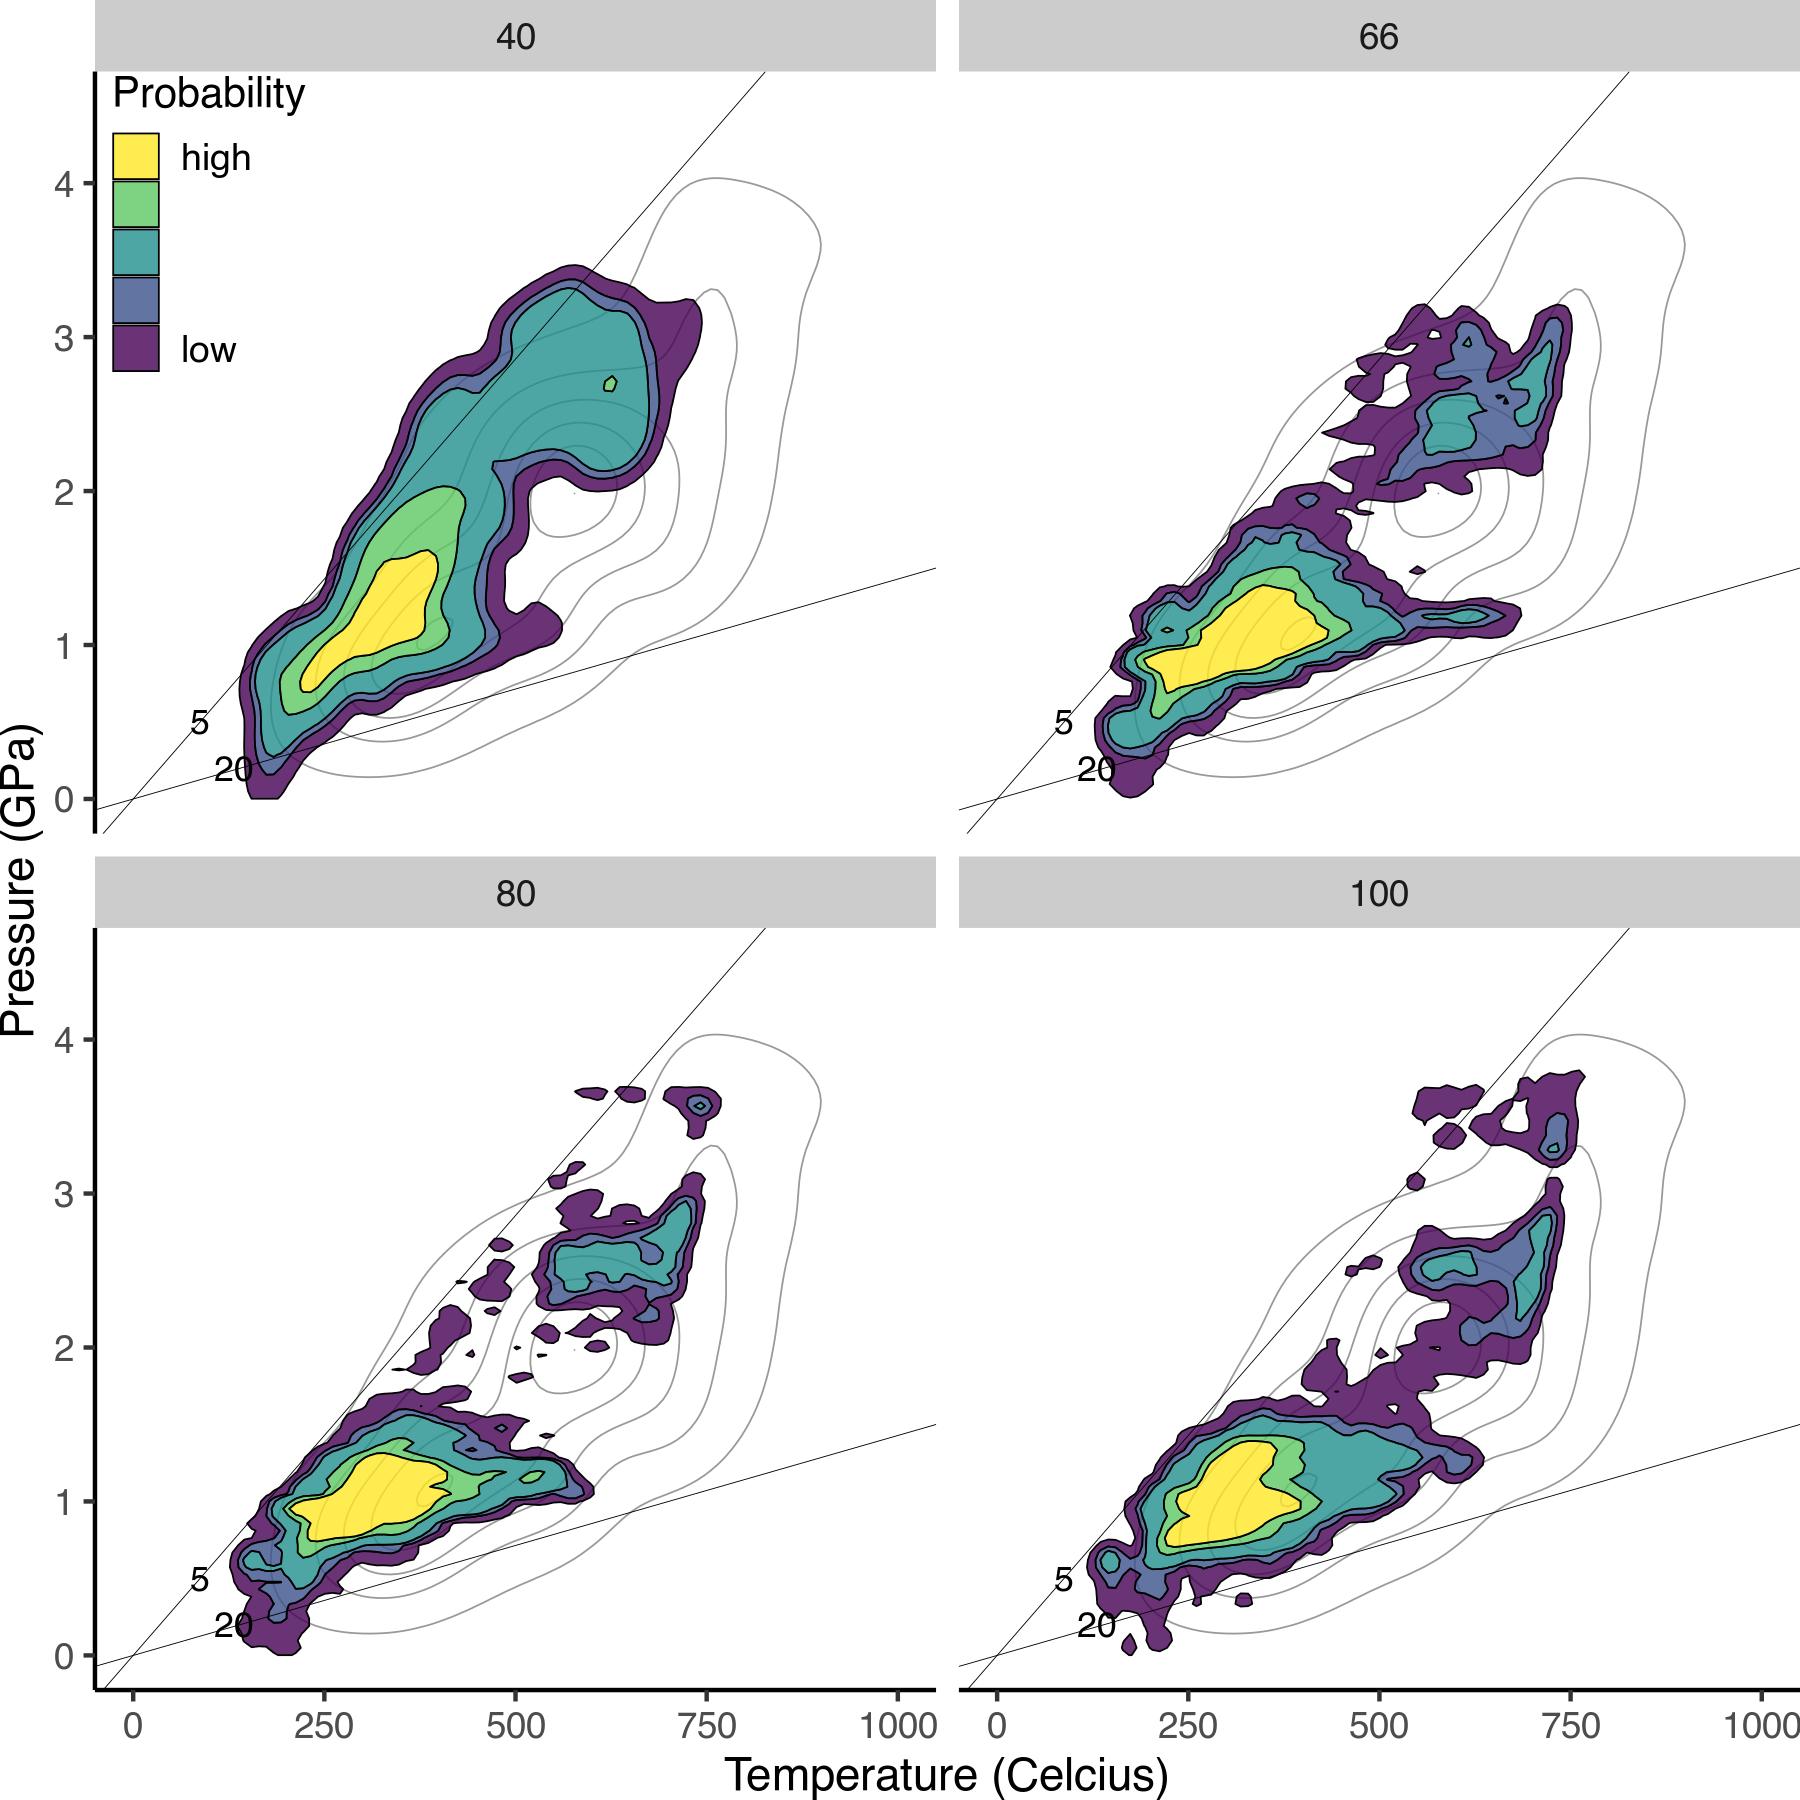
\includegraphics[width=1\linewidth,]{assets/figs/chpt4/cvDensity} 

}

\caption[\gls{pt} distribution of recovered markers by convergence velocity]{\gls{pt} distribution of recovered markers by convergence velocity (panel headers = \(km/Ma\)). Marker \gls{pt} distributions (colored contours) are remarkably different for the lowest-convergence simulations (topleft; 40 \(km/Ma\)) compared to all other convergence rates (\(\geq\) 66 \(km/Ma\)). The slowest-converging simulations recover fewer markers (distribution is smoother) along lower average \gls{pt} gradients, and have more uniform probability density across pressures \(\geq\) 2 \(GPa\). Faster-converging simulations (\(\geq\) 66 \(km/Ma\)) show more segregated distributions with significant gaps in recovery around 2 \(GPa\) (blueschist facies). The rock record (\texttt{pd15}; light gray contours) is most consistent with slow convergence (\(<\) 66 \(km/Ma\)) in terms of probability density but more consistent with the faster convergence (\(\geq\) 66 \(km/Ma\)) in terms of absolute \gls{pt}. An apparent threshold and geodynamic shift exists between velocities of 40 to 66 \(km/Ma\). Thin black lines are average \gls{pt} gradients of 5 \(K/km\) and 20 \(K/km\) (calculated with a lithostatic gradient of 35 \(km/GPa\)).}\label{fig:cvDensity}
\end{figure}

\hypertarget{oceanic-plate-age-effect}{%
\subsubsection{Oceanic-plate Age Effect}\label{oceanic-plate-age-effect}}

Oceanic-plate age has the second strongest effect on marker \gls{pt} distributions, although the effect is relatively small compared to convergence velocity. Older oceanic-plates recover fewer markers from slightly higher average pressures than younger oceanic-plates (Figure \ref{fig:ageDensity}). Significant gaps in the abundances of moderate-P and (ultra-)\gls{hp} rocks appear in simulations across oceanic-plate ages, except for simulations with 85 \(Ma\) plates. Oceanic-plates \(\geq\) 85 \(Ma\) are most consistent with \texttt{pd15}, but still very distinct.



\begin{figure}[htbp]

{\centering 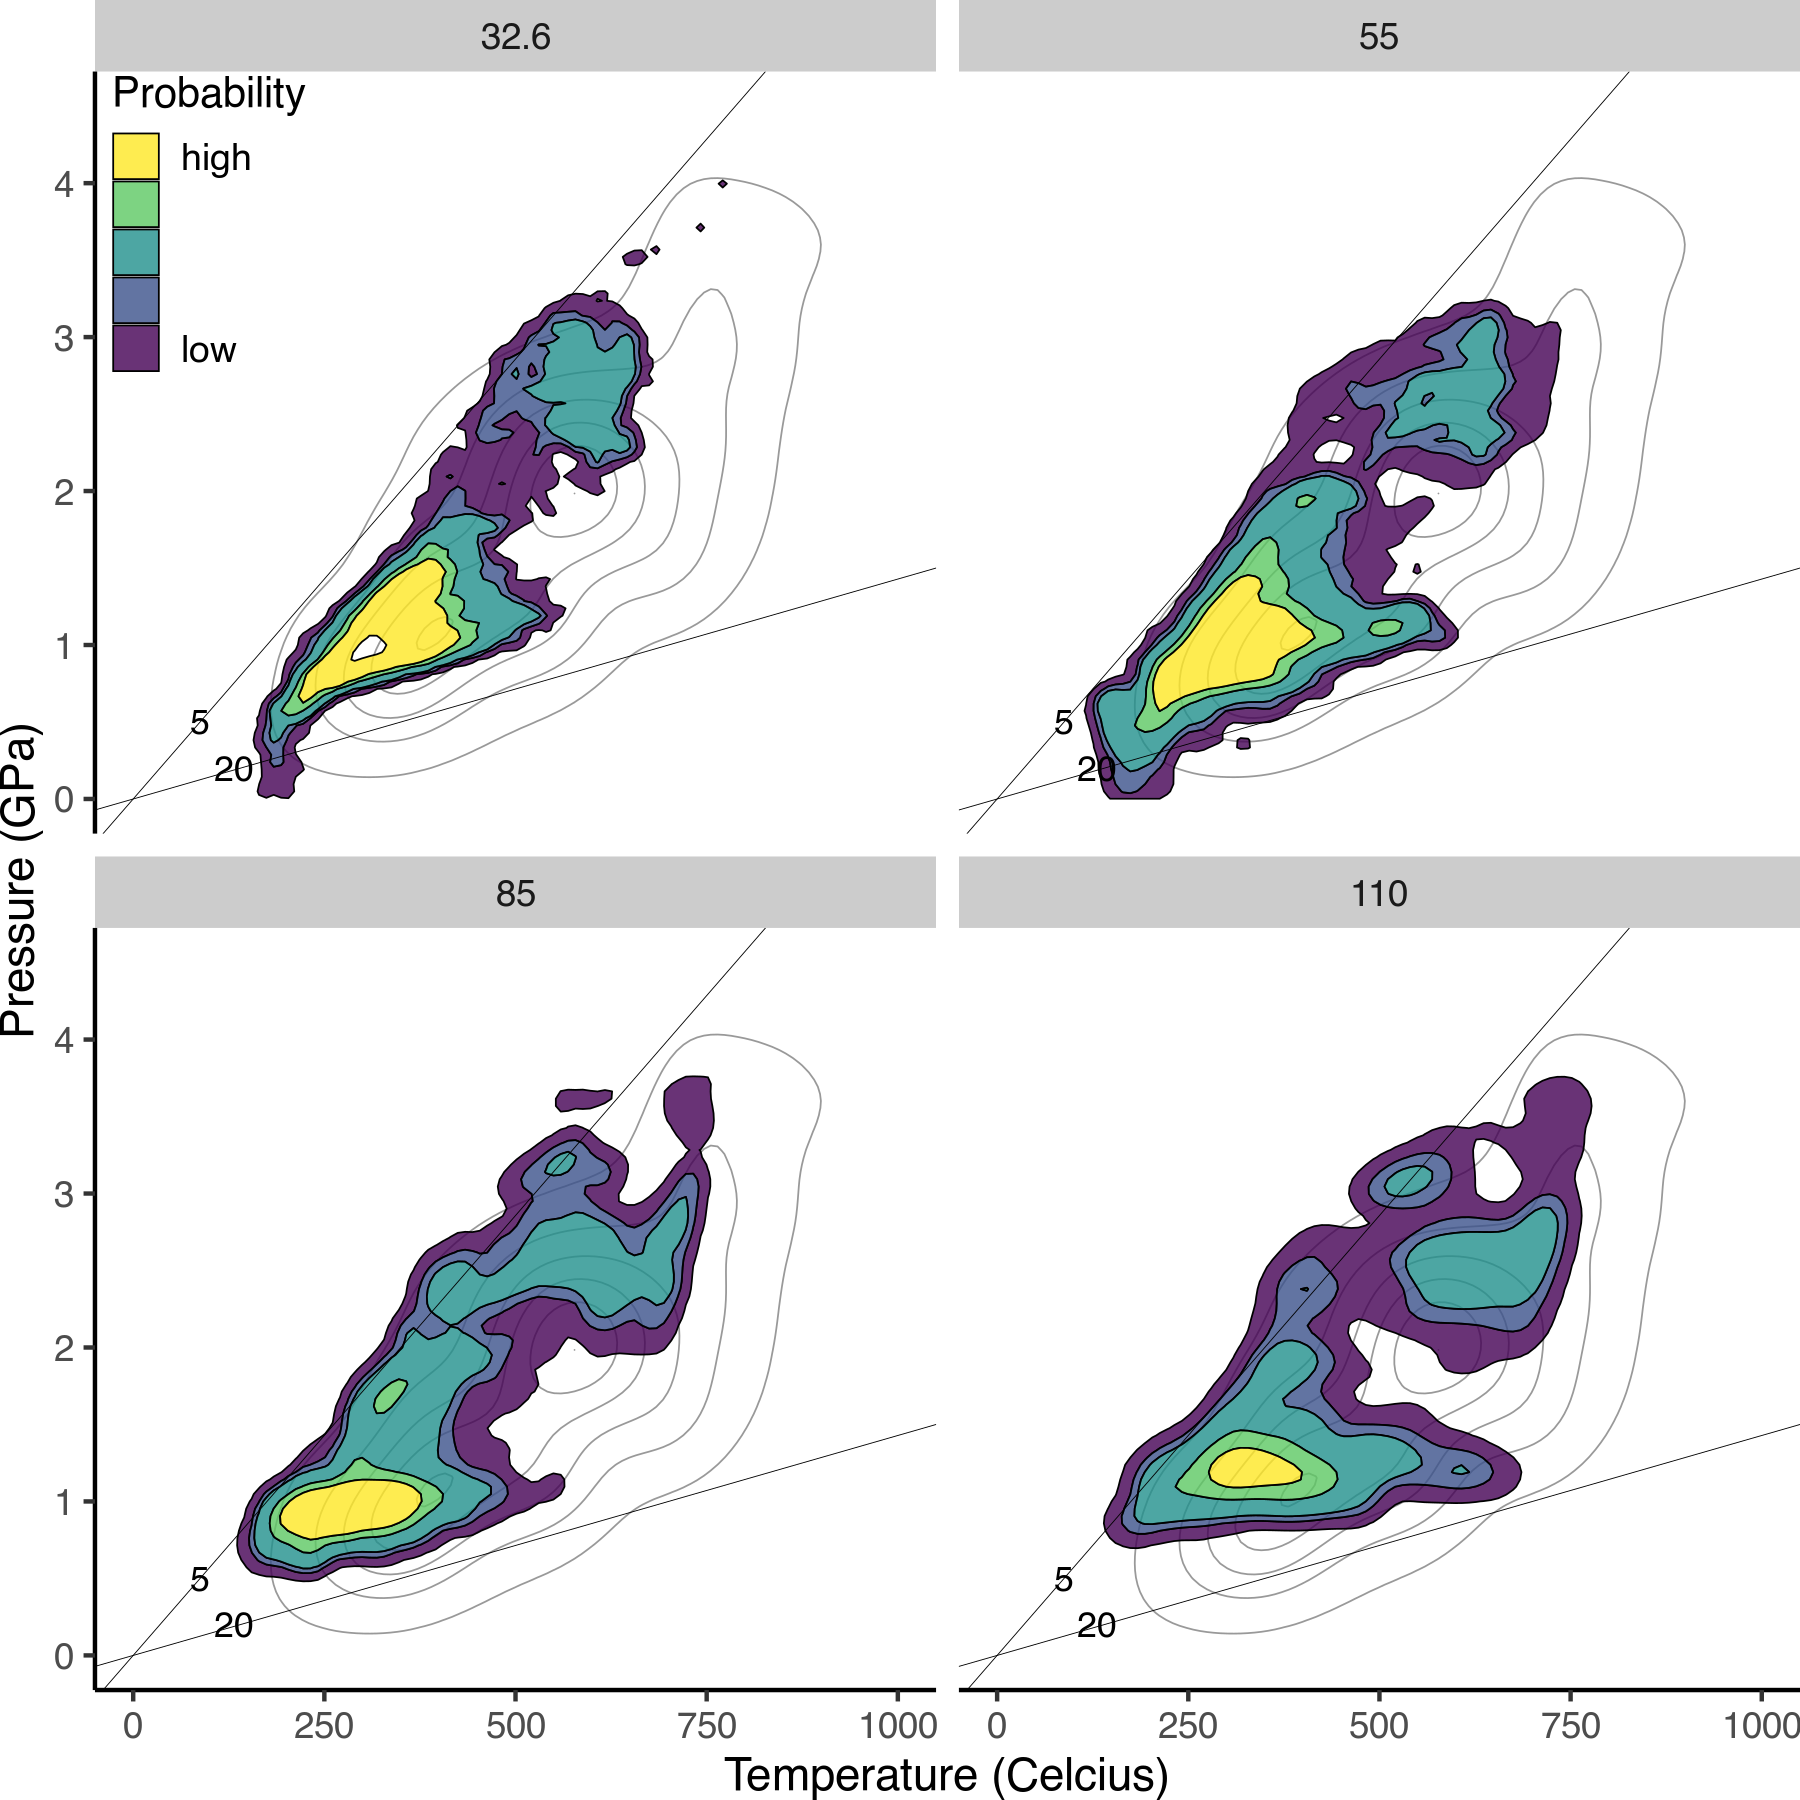
\includegraphics[width=1\linewidth,]{assets/figs/chpt4/ageDensity} 

}

\caption[\gls{pt} distribution of recovered markers by oceanic-plate age]{\gls{pt} distribution of recovered markers by oceanic-plate age (panel headers = \(Ma\)). Marker \gls{pt} distributions (colored contours) show a trend towards lower recovery rates (smoother contours), a shift towards higher average pressures, and more uniform probability density across 1.5 to 2.5 \(GPa\) (lower-blueschist to lower-eclogite facies) with increasing oceanic-plate age. The rock record (\texttt{pd15}; light gray contours) generally agrees more with older oceanic-plates (\(\geq\) 85 \(Ma\)), yet is still distinct. Thin black lines are average \gls{pt} gradients of 5 \(K/km\) and 20 \(K/km\) (calculated with a lithostatic gradient of 35 \(km/GPa\)).}\label{fig:ageDensity}
\end{figure}

\hypertarget{upper-plate-thickness-effect}{%
\subsubsection{Upper-plate Thickness Effect}\label{upper-plate-thickness-effect}}

Chapter \ref{chpt2} demonstrates an association between upper-plate thickness and coupling depth in the same numerical experiments that markers are sampled from (\protect\hyperlink{ref-kerswell2020}{Kerswell et al., 2020} ). \gls{pt} distributions of markers are therefore expected to respond strongly to changes in upper-plate thickness, especially with respect to pressure (depth). However, a surprisingly modest effect is observed (Figure \ref{fig:zupDensity}). Marker density transitions towards more uniform distributions and higher top-end pressures with increasing upper-plate thickness, while average \gls{pt} gradients significantly decrease. The shift towards more abundant (ultra-)\gls{hp} rocks with increasing upper-plate thickness is more modest than anticipated from Chapter \ref{chpt2} but still consistent with a general increase in mechanical coupling depth with increasing upper-plate thickness (\protect\hyperlink{ref-kerswell2020}{Kerswell et al., 2020}; \protect\hyperlink{ref-ruh2015}{Ruh et al., 2015}).

Notably, markers recovered from simulations with thin upper-plates (\(\leq\) 62 \(km\)) match \texttt{pd15} well in terms of \emph{absolute} \gls{pt} distribution. Yet, marker densities draw the opposite association (thicker upper-plates are most consistent with \texttt{pd15}). A noticeable absence of markers recovered from pressures of approximately 2 \(GPa\) in simulations with thin upper-plates is also inconsistent with \texttt{pd15}, which has a modest-probability hill around 2 \(GPa\) where relatively few markers get recovered.



\begin{figure}[htbp]

{\centering 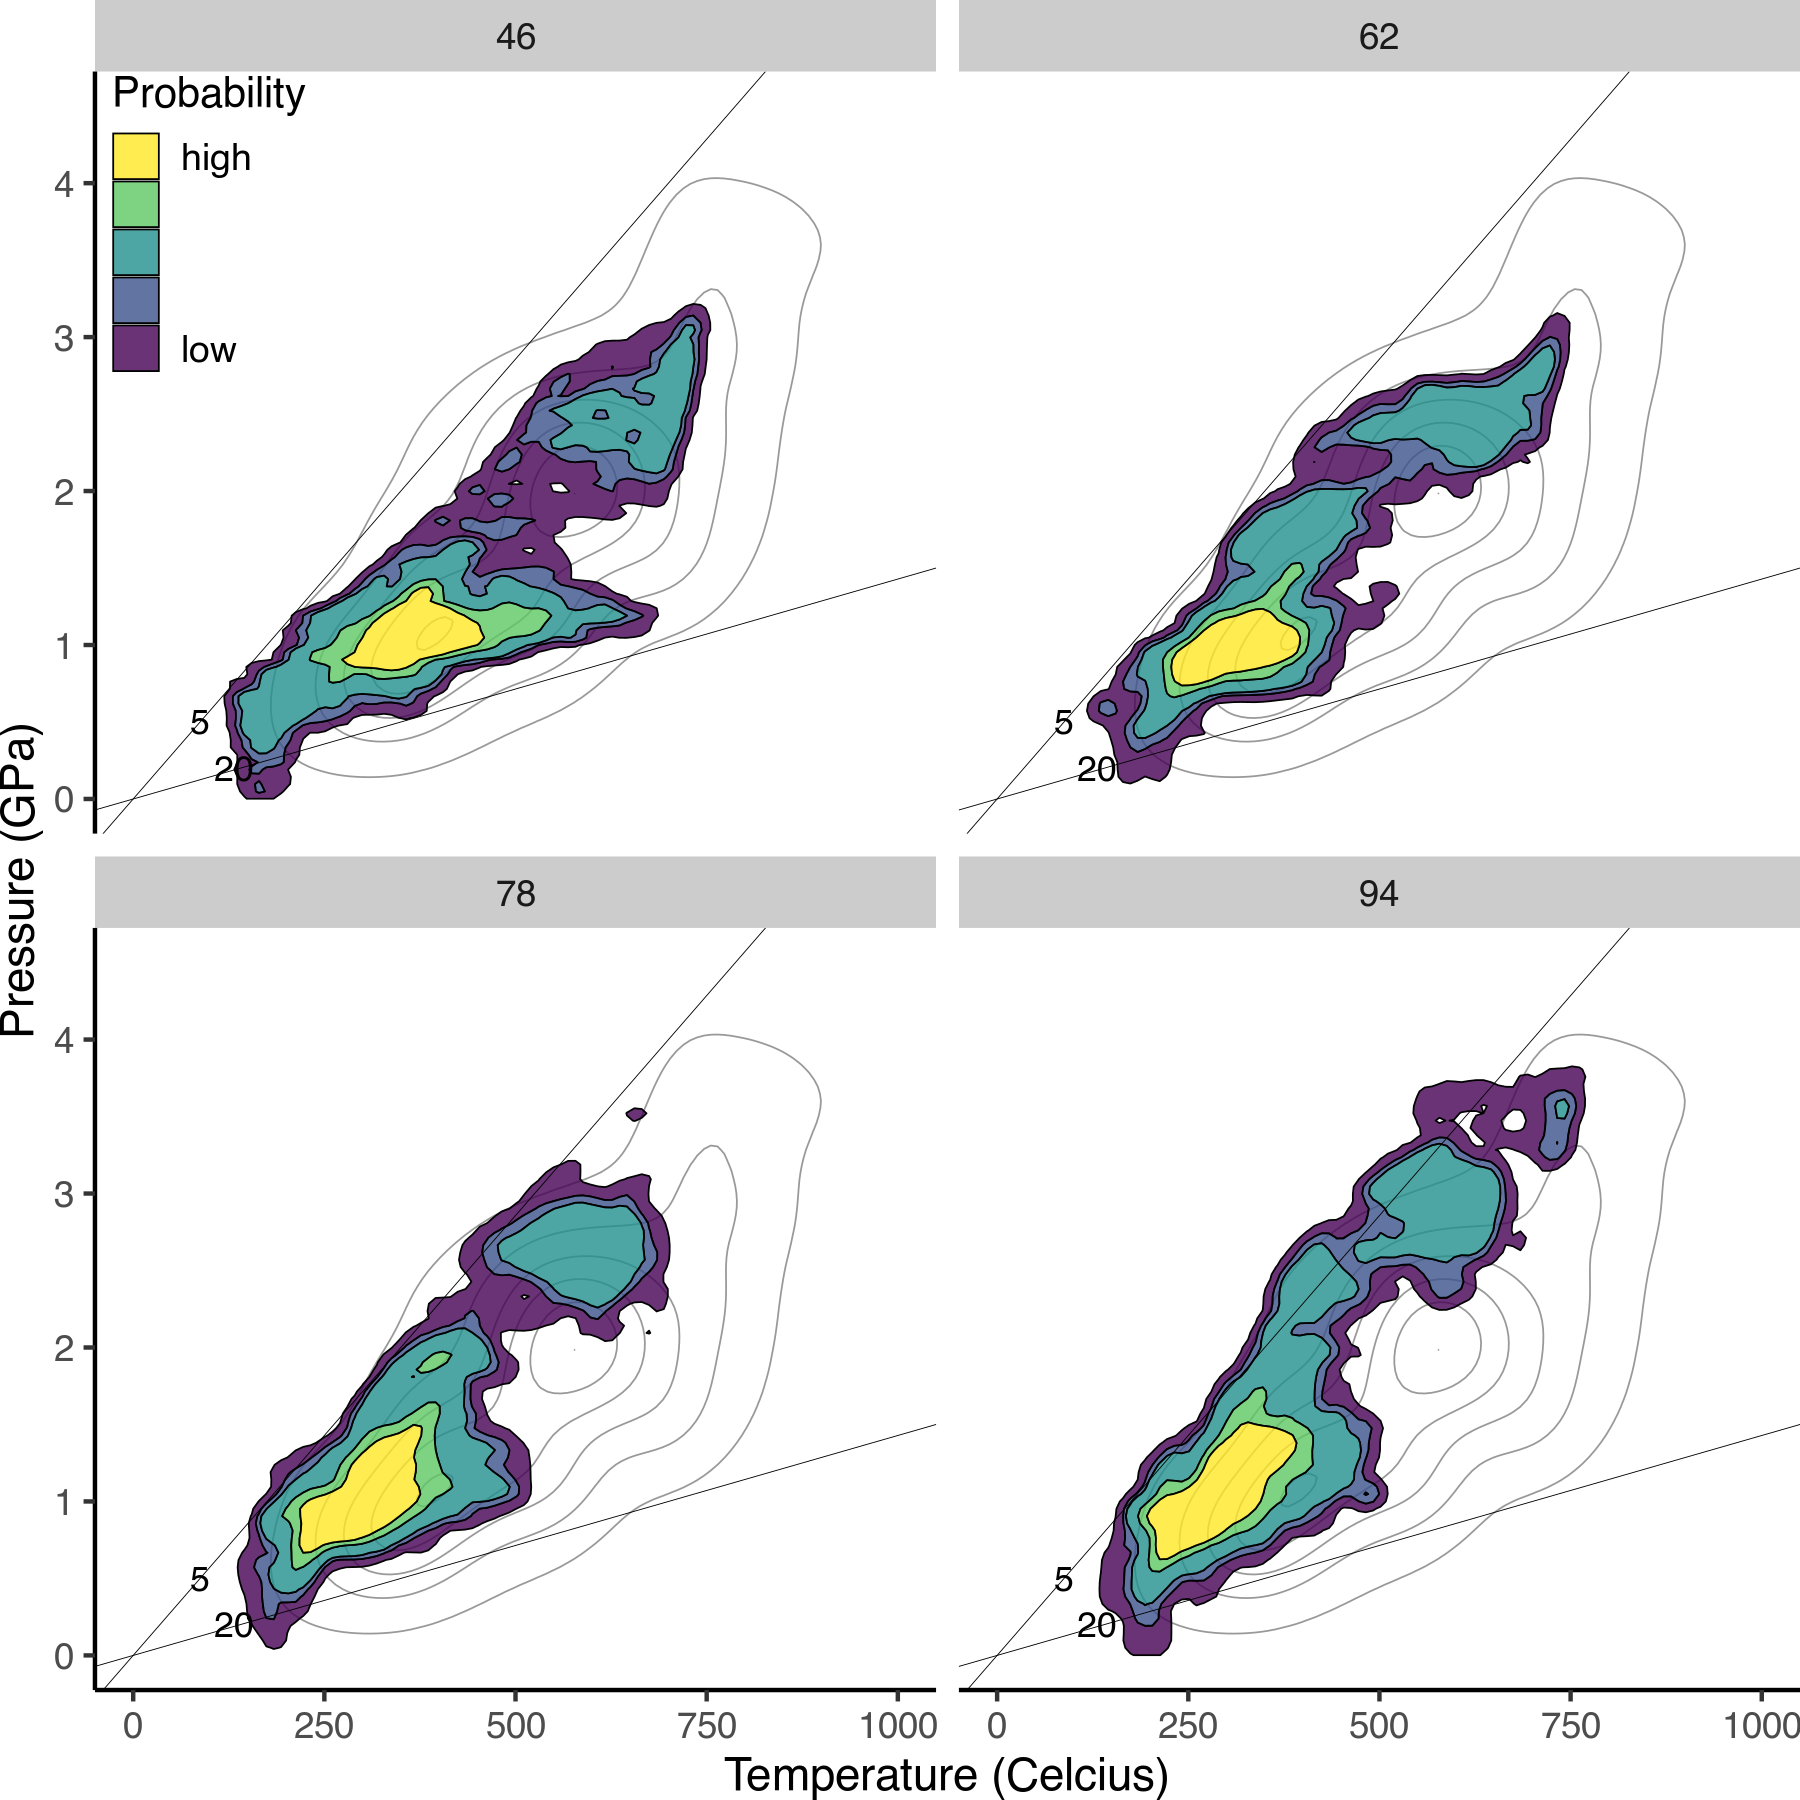
\includegraphics[width=1\linewidth,]{assets/figs/chpt4/zupDensity} 

}

\caption[Marker PT distribution by upper-plate thickness]{\gls{pt} distribution of recovered markers by upper-plate lithospheric thickness (panel headers = \(km\)). Marker \gls{pt} distributions (colored contours) become marginally more uniform and have lower average \gls{pt} gradients with increasing upper-plate thickness. The rock record (\texttt{pd15}; light gray contours) is most consistent with thin upper-plates (\(\leq\) 62 \(km\)) in terms of absolute \gls{pt} distribution. Regardless of upper-plate thickness, relatively few markers are recovered from pressures around 2 \(GPa\) compared to the rock record. In general, upper-plate thickness has a surprisingly small effect on the \gls{pt} distribution of recovered markers with respect to pressure. Thin black lines are average \gls{pt} gradients of 5 \(K/km\) and 20 \(K/km\) (calculated with a lithostatic gradient of 35 \(km/GPa\)).}\label{fig:zupDensity}
\end{figure}

\hypertarget{detachment-timing-effect}{%
\subsubsection{Detachment Timing Effect}\label{detachment-timing-effect}}

Figure \ref{fig:detachDensity} shows marker \gls{pt} distributions at 10 percent increments of total subduction duration. Marker recovery exhibits three trends with respect to time. First, marker recovery rates decrease through time with a substantial drop after approximately 40\% of total subduction duration. Second, average \gls{pt} gradients rotate anti-clockwise from approximately 10-15 to 5 \(K/km\) after 50\% of total subduction duration. Finally, markers are recovered from increasingly higher pressures beginning from 0.2-1.3 to 3.5 \(GPa\) by 40\% of total subduction duration. Secular trends in marker recovery show significant low-P, moderate- to high-T marker recovery (greenschist to amphibolite facies) during the first 30-40\% of the subduction life-cycle, followed by a higher relative proportion of (ultra-)\gls{hp} markers (blueschist and eclogites). Absolute \gls{pt} trends are most consistent with \texttt{pd15} during the first third of the subduction life-cycle, but marker probability density is most consistent with \texttt{pd15} during the final half of the subduction life-cycle.



\begin{figure}[htbp]

{\centering 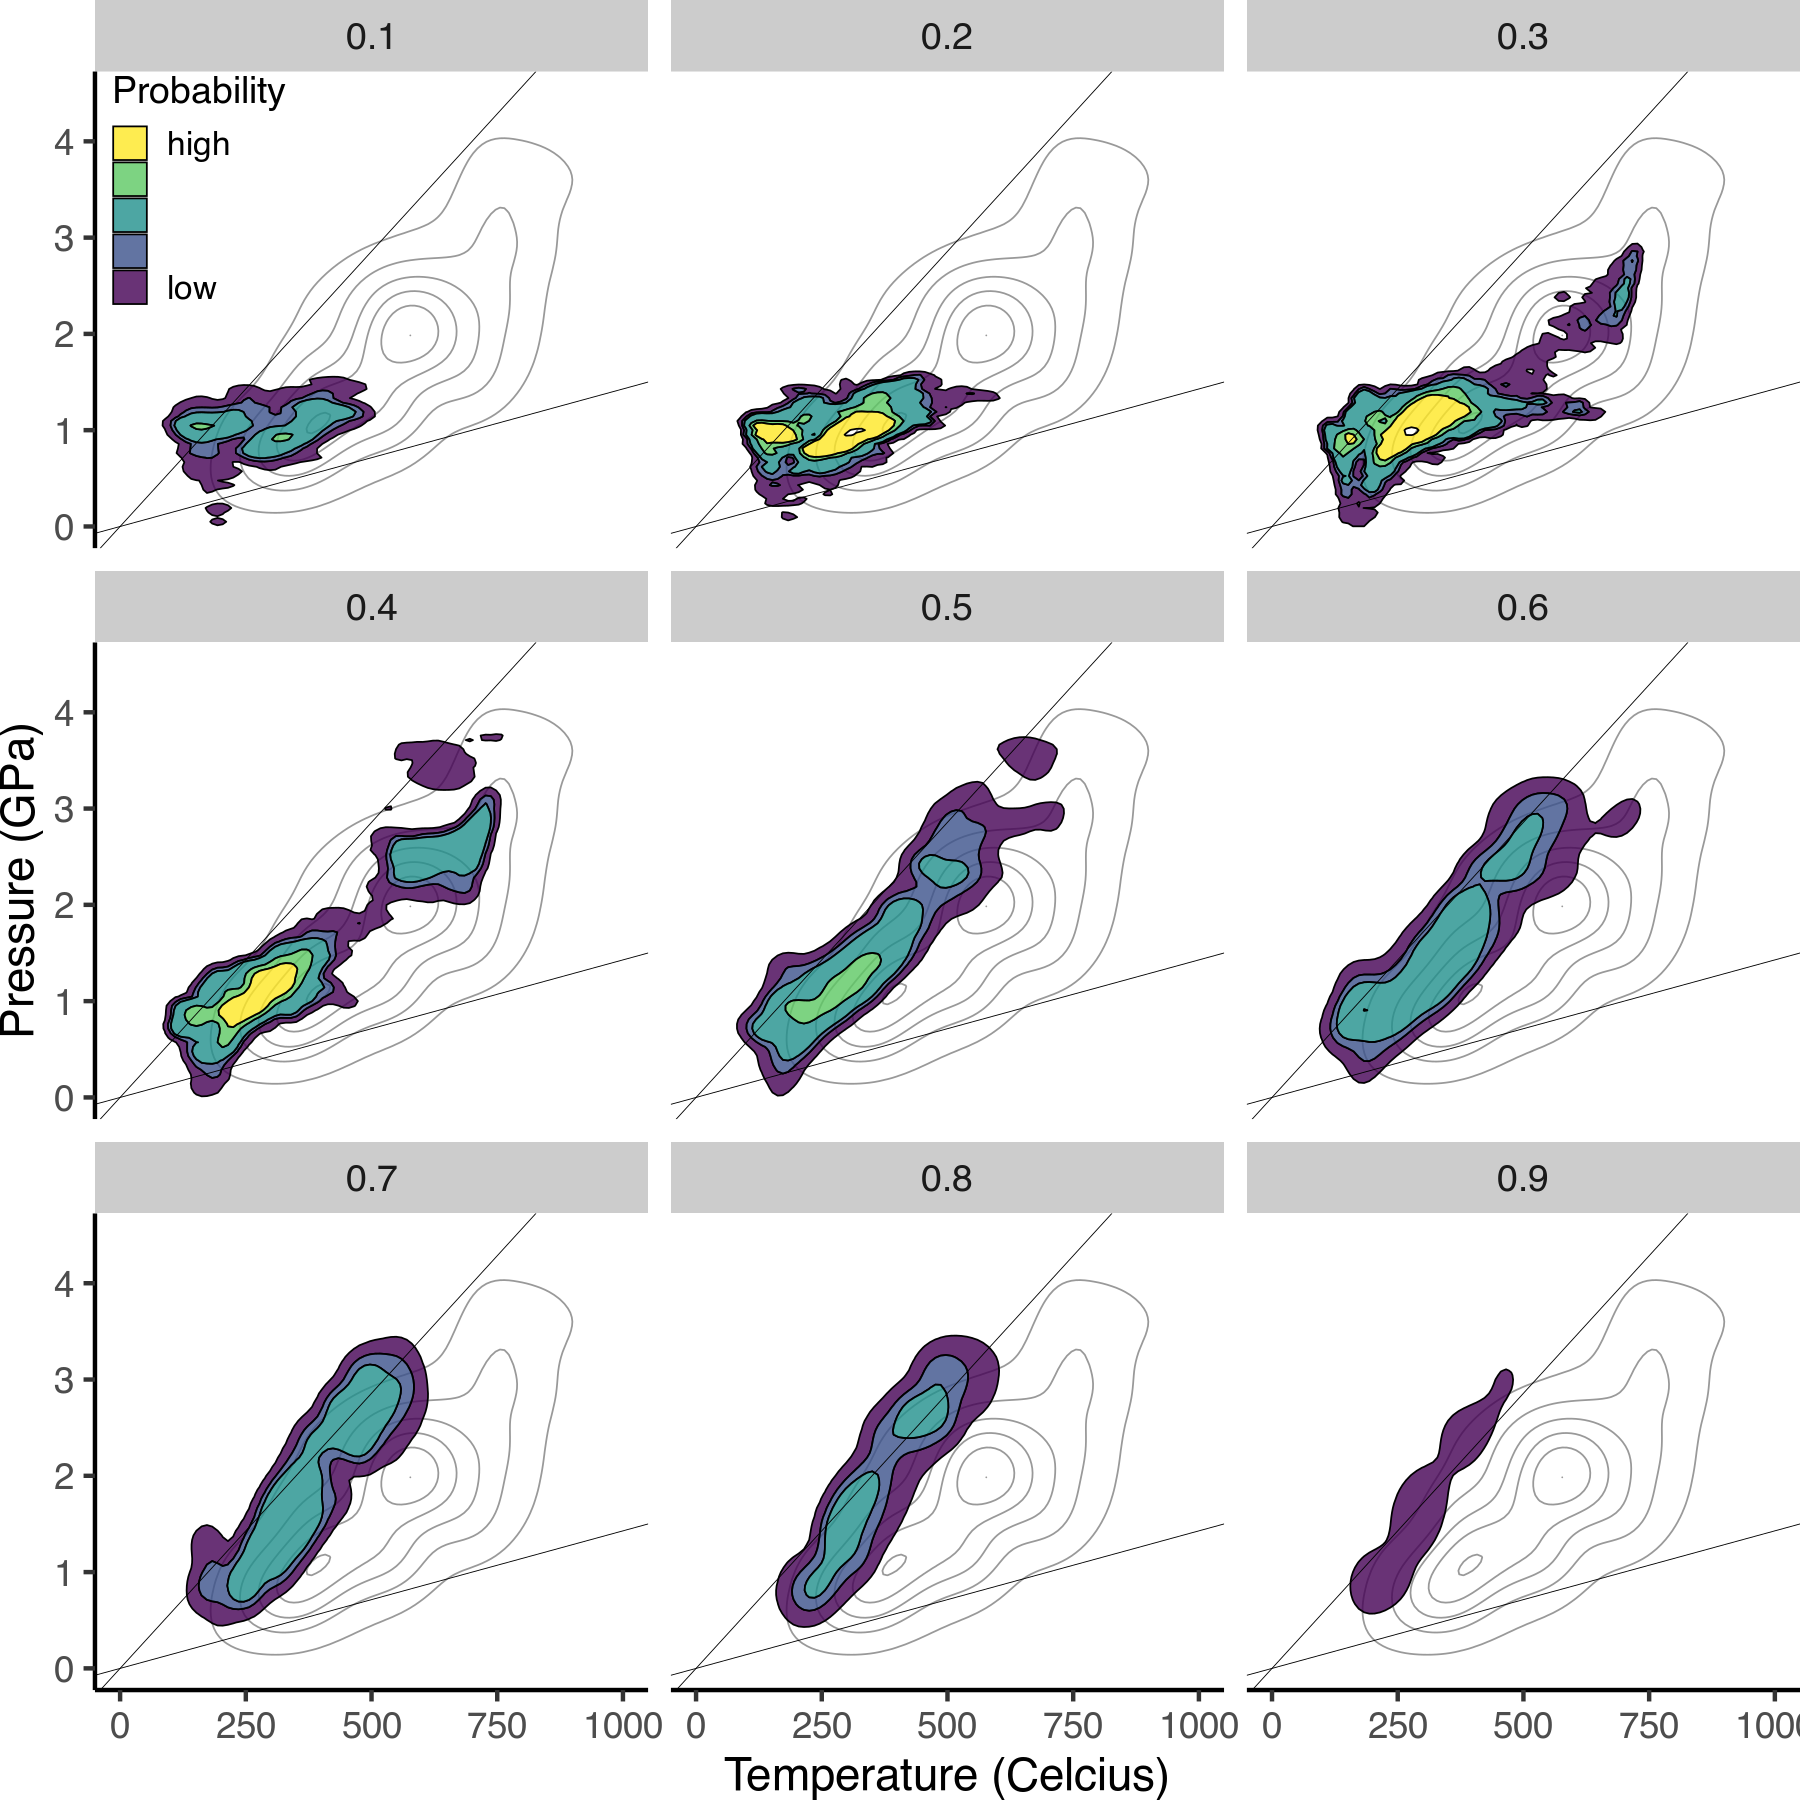
\includegraphics[width=1\linewidth,]{assets/figs/chpt4/detachDensity} 

}

\caption[Marker PT distribution by relative detachment timing]{\gls{pt} distribution of recovered markers by relative detachment timing (panel headers = 10\% increments of total subduction duration). Marker \gls{pt} distributions (colored contours) are restricted to lower-P, moderate- to higher-T conditions through the first third of the subduction life-cycle. Average \gls{pt} gradients then progressively rotate towards cooler conditions while recovery extends to higher pressures through time (\(\geq\) 0.3). Recovery rates continuously fall (contours get smoother) through time with a significant decrease after approximately 40\% of the subduction life-cycle has passed. Absolute \gls{pt} and probability distributions are both time-dependent. Gray contours represent the \gls{pt} distribution of the rock record (\texttt{pd15}). Thin black lines are average \gls{pt} gradients of 5 \(K/km\) and 20 \(K/km\) (calculated with a lithostatic gradient of 35 \(km/GPa\)).}\label{fig:detachDensity}
\end{figure}

\hypertarget{recovery-rates}{%
\subsection{Recovery Rates}\label{recovery-rates}}

A notable pattern emerges when comparing recovery rates among all 64 subduction simulations by thermo-kinematic boundary conditions (Figure \ref{fig:recRate}). Simulations with younger and more slowly converging oceanic-plates (low-\(\Phi\)) have higher recovery rates than older and more quickly converging oceanic-plates (high-\(\Phi\)). This negative correlation between \(\Phi\) and recovery rate appears gradual and continuous. In contrast, no apparent correlation exists between recovery rate and upper-plate lithospheric thickness. Please also note that low-\(\Phi\) simulations generally appear to have broader distributions of marker recovery across pressure in addition to higher recovery rates (Figure \ref{fig:recRate}).

On average 7.5 percent of markers get recovered from subduction (Table \ref{tab:recSummary}). While volumes of rock cannot be directly computed from recovery rates because markers are mathematical point features, volumes may be roughly estimated by assuming markers represent the entire 760 \(\times\) 8 \(km\) section of oceanic crust and seafloor sediments they were sampled from. Rates of subducted material then range from 5,285 to 6,080 \(km^3/km\), with a mean of 5,622 \(km^3/km\). Rates of recovered material range from 0 to 795 \(km^3/km\), with a mean of 458 \(km^3/km\).



\begin{figure}[htbp]

{\centering 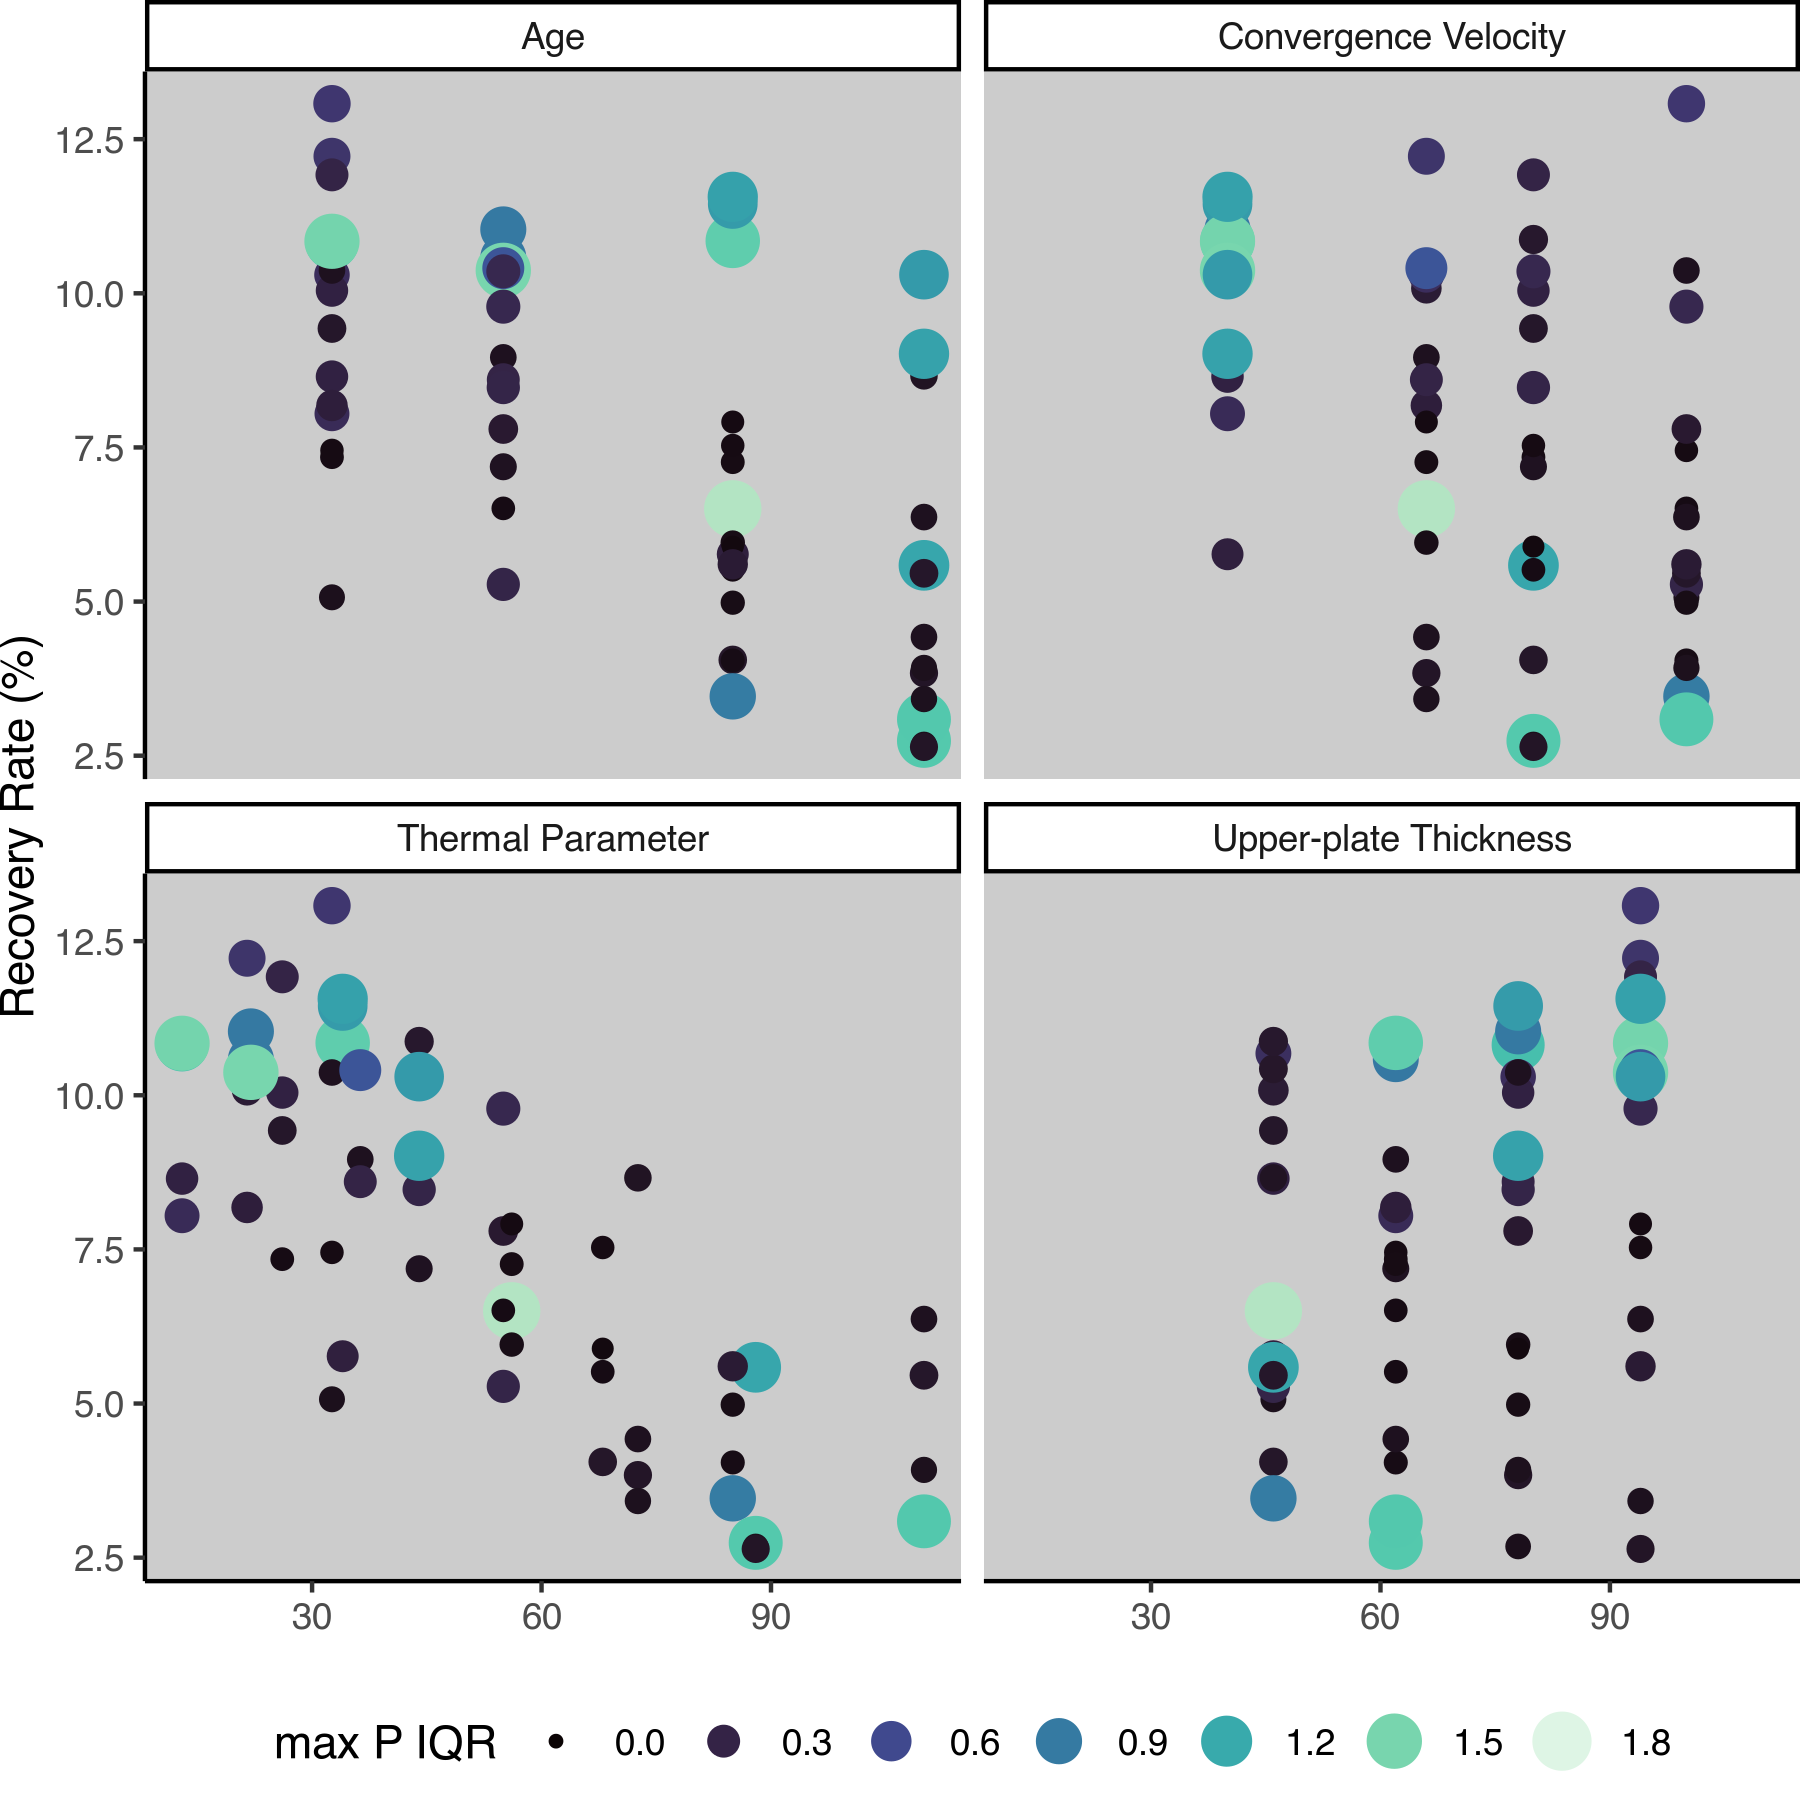
\includegraphics[width=1\linewidth,]{assets/figs/chpt4/recRate} 

}

\caption[Recovery rates for all 64 subduction simulations]{Recovery rates for all 64 subduction simulations by thermo-kinematic boundary conditions. Negative correlations are observed among recovery rate, oceanic-plate age (\(Ma\)), convergence velocity (\(km/Ma\)), and thermal parameter (\(\Phi\); \(km/100\)). Note that \(\Phi\) is simply the product of oceanic-plate age and convergence velocity. No apparent correlation is observed between recovery rate and upper-plate thickness (\(km\)). Data point size and color represent the interquartile range of maximum marker pressures (\(GPa\)). The youngest and slowest-moving oceanic-plates generally have the highest recovery rates and marker recovery across broader ranges of pressures.}\label{fig:recRate}
\end{figure}

\hypertarget{chpt4Discussion}{%
\section{Discussion}\label{chpt4Discussion}}

\hypertarget{recovery-rates-1}{%
\subsection{Recovery Rates}\label{recovery-rates-1}}

Marker recovery rates show a smooth negative correlation with \(\Phi\) and no correlation with upper-plate thickness (Figure \ref{fig:recRate}). Geodynamic factors contributing to this association are difficult to deduce, however, partly because \(\Phi\) itself was formulated from a general relationship among thermo-kinematic boundary conditions to explain differences in earthquake distributions among subduction zones (\protect\hyperlink{ref-gorbatov1997}{Gorbatov \& Kostoglodov, 1997}; \protect\hyperlink{ref-kirby1991}{Kirby et al., 1991}; \protect\hyperlink{ref-mckenzie1969}{McKenzie, 1969}; \protect\hyperlink{ref-molnar1979}{Molnar et al., 1979}), and likely never intended as a precise tool for investigating subduction geodynamics. Notwithstanding, oceanic-plate age appears to explain most of the correlation between recovery rates and \(\Phi\). Average recovery rate drops systematically with increasing oceanic-plate age. In contrast, only the slowest-converging simulations (40 \(km/Ma\)) appear to have distinct recovery rates compared to more quickly-converging simulations (\(\geq\) 66 \(km/Ma\); Figure \ref{fig:recRate}).

A common observation among simulations with young oceanic-plates, especially at slow convergence rates, are high subduction angles. Moreover, simulations with high subduction angles tend to create more space for underplating detached material (see Figure \ref{fig:geodyn}, discussed below). These observations imply recovery rates respond to \(\Phi\) because of differences in plate flexibility and overall subduction geometry, rather than oceanic-plate age and convergence velocity \emph{per se}. Please note, however, that subduction angle appears to be most strongly correlated with subduction duration compared to other thermo-kinematic boundary conditions (\protect\hyperlink{ref-hu2020}{Hu \& Gurnis, 2020}). Drawing a relationship among \(\Phi\), subduction angle, and recovery rates, without also considering subduction duration, is therefore inconclusive. Recovery rates may obviously correlate with \(\Phi\), but a concrete explanation is difficult to untangle.

\hypertarget{pt-distributions}{%
\subsection{PT Distributions}\label{pt-distributions}}

Although \gls{pt} distributions of recovered markers for some simulations are consistent with \texttt{pd15} in absolute terms, probability densities bear little resemblance to \texttt{pd15} for most simulations. From an absolute perspective, marker \gls{pt} distributions from simulations with moderate to fast convergence velocities (\(\geq\) 66 \(km/Ma\); Figure \ref{fig:cvDensity}), older oceanic-plates (\(\geq\) 85 \(Ma\); Figure \ref{fig:ageDensity}), or thin upper-plates (\(\leq\) 62 \(km\); Figure \ref{fig:zupDensity}) could be considered consistent with \texttt{pd15}. However, it would be very unlikely to reproduce \texttt{pd15} by randomly sampling markers from the above simulations. Only the slowest-converging simulations recover \gls{hp} rocks with similar relative frequency across pressures of \(\sim\) 0.8 to 2.4 \(GPa\) compared to \texttt{pd15} (Figure \ref{fig:ecdfs}).



\begin{figure}[htbp]

{\centering 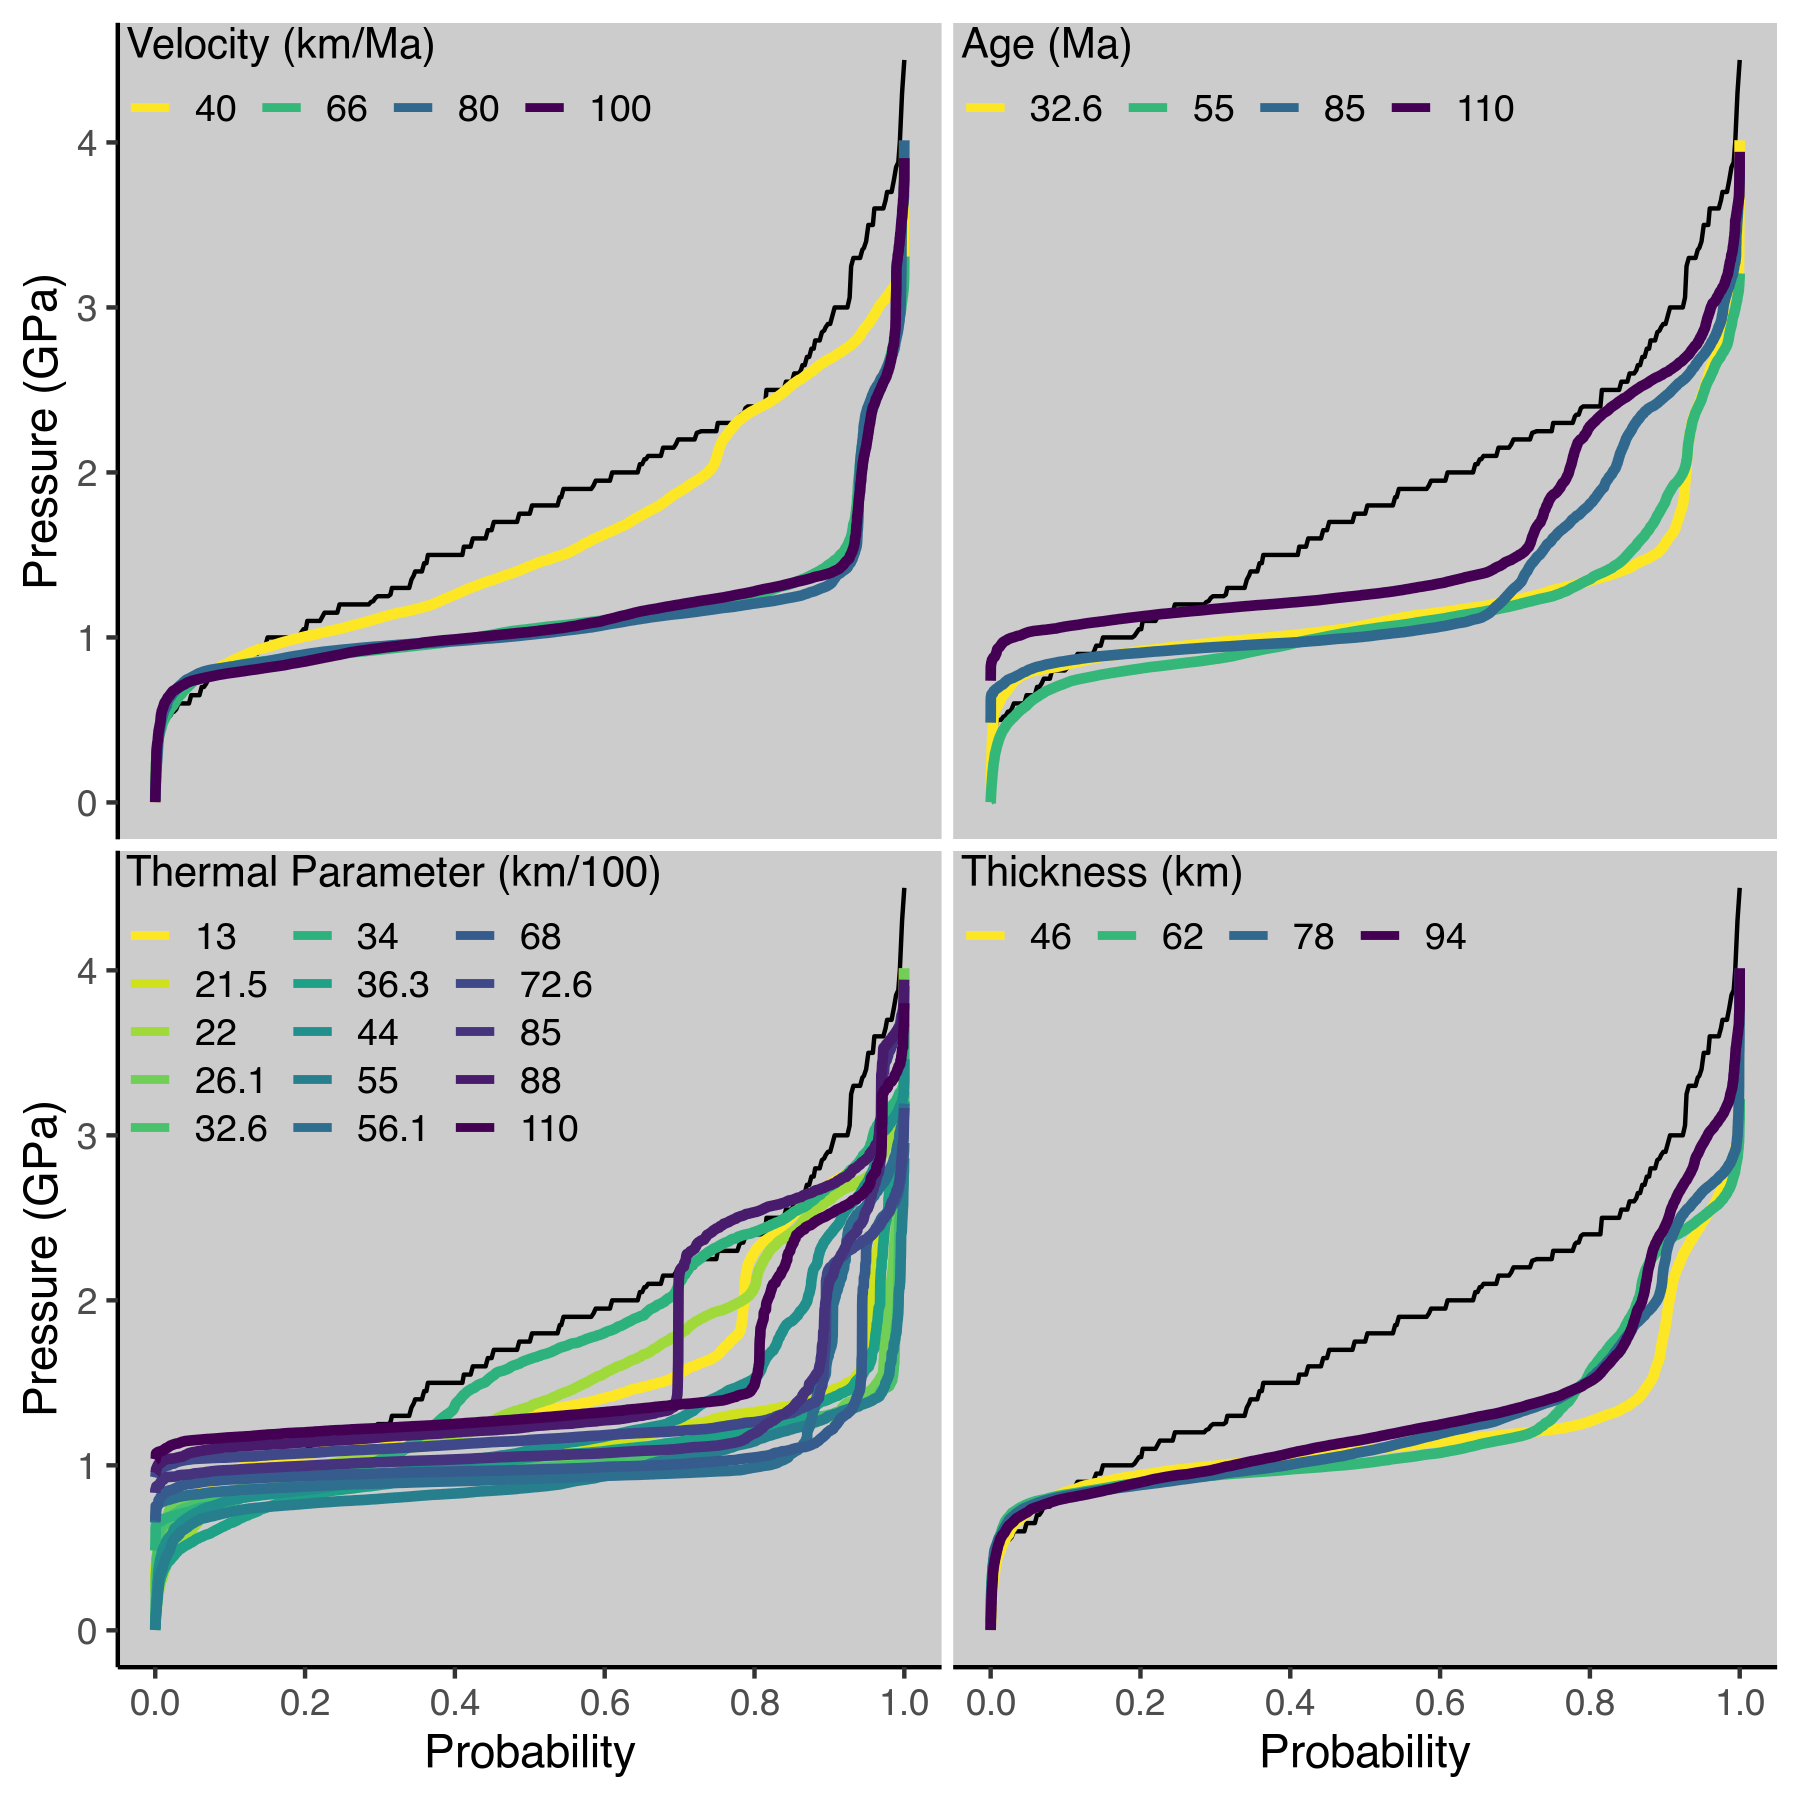
\includegraphics[width=1\linewidth,]{assets/figs/chpt4/ecdfs} 

}

\caption[Cumulative probability distributions of marker `maxP` by thermo-kinematic initial conditions]{Coupling depths of recovered marker pressures by thermo-kinematic boundary conditions. Convergence velocity has the largest effect on the pressure distributions of recovered markers (topleft). Only the slowest-converging simulations (40 \(km/Ma\)) resemble the rock record (\texttt{pd15}; thin jagged black line) and are distinct from faster-converging simulations (\(\geq\) 66 \(km/Ma\)), implying a geodynamic shift towards more discrete recovery along the plate interface at \textgreater{} 40 \(km/Ma\). Oceanic-plate ages have a moderate effect on marker recovery, with older plates recovering more markers from 1.5 to 2.5 \(GPa\) (topright). The thermal parameter shows a range of marker distributions that reflect the combined effects of convergence velocity and age (bottomleft). Upper-plate thickness has surprisingly little effect on marker recovery (bottomright). Regardless of thermo-kinematic boundary conditions, most simulations present distributions that do overlap with \texttt{pd15}. \gls{hp} rocks between 0.8 and 2.4 \(GPa\) are overrepresented in \texttt{pd15} compared to most simulations.}\label{fig:ecdfs}
\end{figure}

The fact that very few simulations recover as many markers from 0.8 to 2.4 \(GPa\) compared to \texttt{pd15}, except for the slowest-converging systems (Figure \ref{fig:ecdfs}), is a key result of this study. Different possible interpretations may follow from this observation. For example, the rock record may be comprised of \gls{hp} rocks mostly recovered from slowly-converging subduction zones. Alternatively, the rock record may not reflect the true distribution of \gls{hp} rocks recovered in subduction zones and is overrepresented (biased) by \gls{hp} rocks between 0.8 to 2.4 \(GPa\). A simple calculation may test the former interpretation:

\begin{quote}
One-half of modern day subduction zone segments have estimated convergence velocities below 66 \(km/Ma\) (\protect\hyperlink{ref-syracuse2010}{Syracuse et al., 2010}). As a conservative estimate, the prior probability of sampling a \gls{hp} rock from a slowly-converging system is around 50\%, assuming the proportion of slowly-converging systems is constant through time and recovery rates are equal among subduction zones. So the chance of sampling a \gls{hp} rock from a slowly-converging system is not exceedingly small. However, the probability that half (n = 130) of \gls{hp} rocks in \texttt{pd15} with pressure estimates between 0.8 and 2.4 \(GPa\) (n = 260) were sampled from slowly-converging systems can be approximated by a binomial probability distribution:
\DIFdelbegin %DIFDELCMD < 

%DIFDELCMD < %%%
\DIFdelend \begin{equation}P(k) = B\left(n \atop k \right)\ p^k\ q^{n-k} = B\left(260 \atop 130 \right)\ 0.5^{130}\ 0.5^{130} \approx 5\% \label{eq:binom} \end{equation}
\DIFdelbegin %DIFDELCMD < 

%DIFDELCMD < %%%
\DIFdelend where \(P(k)\) is the probability of sampling \(k=130\) \gls{hp} rocks from \(n=260\) trials, \(B\left( n \atop k \right) = n!/k!(n-k)!\) is the binomial distribution, and \(p\) and \(q\) are the chances of sampling a \gls{hp} frock from a slowly-converging system and not sampling a \gls{hp} rock, respectively.
\end{quote}

In other words, there is a 5\% chance that 130/260 \gls{hp} rocks in \texttt{pd15} were sampled exclusively from slowly-converging (\(\leq\) 66 \(km/Ma\)) subduction zones. It is therefore unlikely that \texttt{pd15} represents preferential sampling of \gls{hp} rocks from only slowly-converging subduction zones (the same principle can also be applied to other thermo-kinematic boundary conditions). Rather, it is much more likely that \texttt{pd15} reflects an overabundance of undifferentiated samples between 0.8 and 2.4 \(GPa\). While the true distribution of \gls{hp} rock recovered globally cannot be known, rough calculations demonstrating the improbability of preferential sampling from a subset of subduction zones and a general inconsistency among marker \gls{pt} distributions and the rock record stress the importance of differentiating \gls{pt} estimates with relevant metadata. For example, sorting aggregated suites of \gls{hp} rocks by like metamorphic ages, lithologies, and estimates for thermo-kinematic boundary conditions (e.g., \protect\hyperlink{ref-agard2018}{Agard et al., 2018}), make for better comparisons with natural and simulated \gls{ptt} datasets.

\hypertarget{geodynamics}{%
\subsection{Geodynamic regimes}\label{geodynamics}}

Marker motions are constrained by a high-viscosity wedge of upper mantle in the forearc region (known as the \emph{cold nose}) and a low-viscosity serpentinized subduction channel (see Appendix \ref{vis}). Four geodynamic regimes are observed across all 64 simulations, each with a different channel geometry and pressure distribution of recovered markers (Figure \ref{fig:geodyn}). Thick, rigid oceanic-plates, especially converging at high velocities (high-\(\Phi\)), tend to have low subduction angles and narrow subduction channels. Most markers are recovered at the base of the accretionary prism and no eclogites are recovered. These simulations imply systems with low subduction angles are expected to have low recovery rates from pressures \(\geq\) 1.5 \(GPa\) (Figure \ref{fig:geodyn}, cdh94).



\begin{figure}[htbp]

{\centering 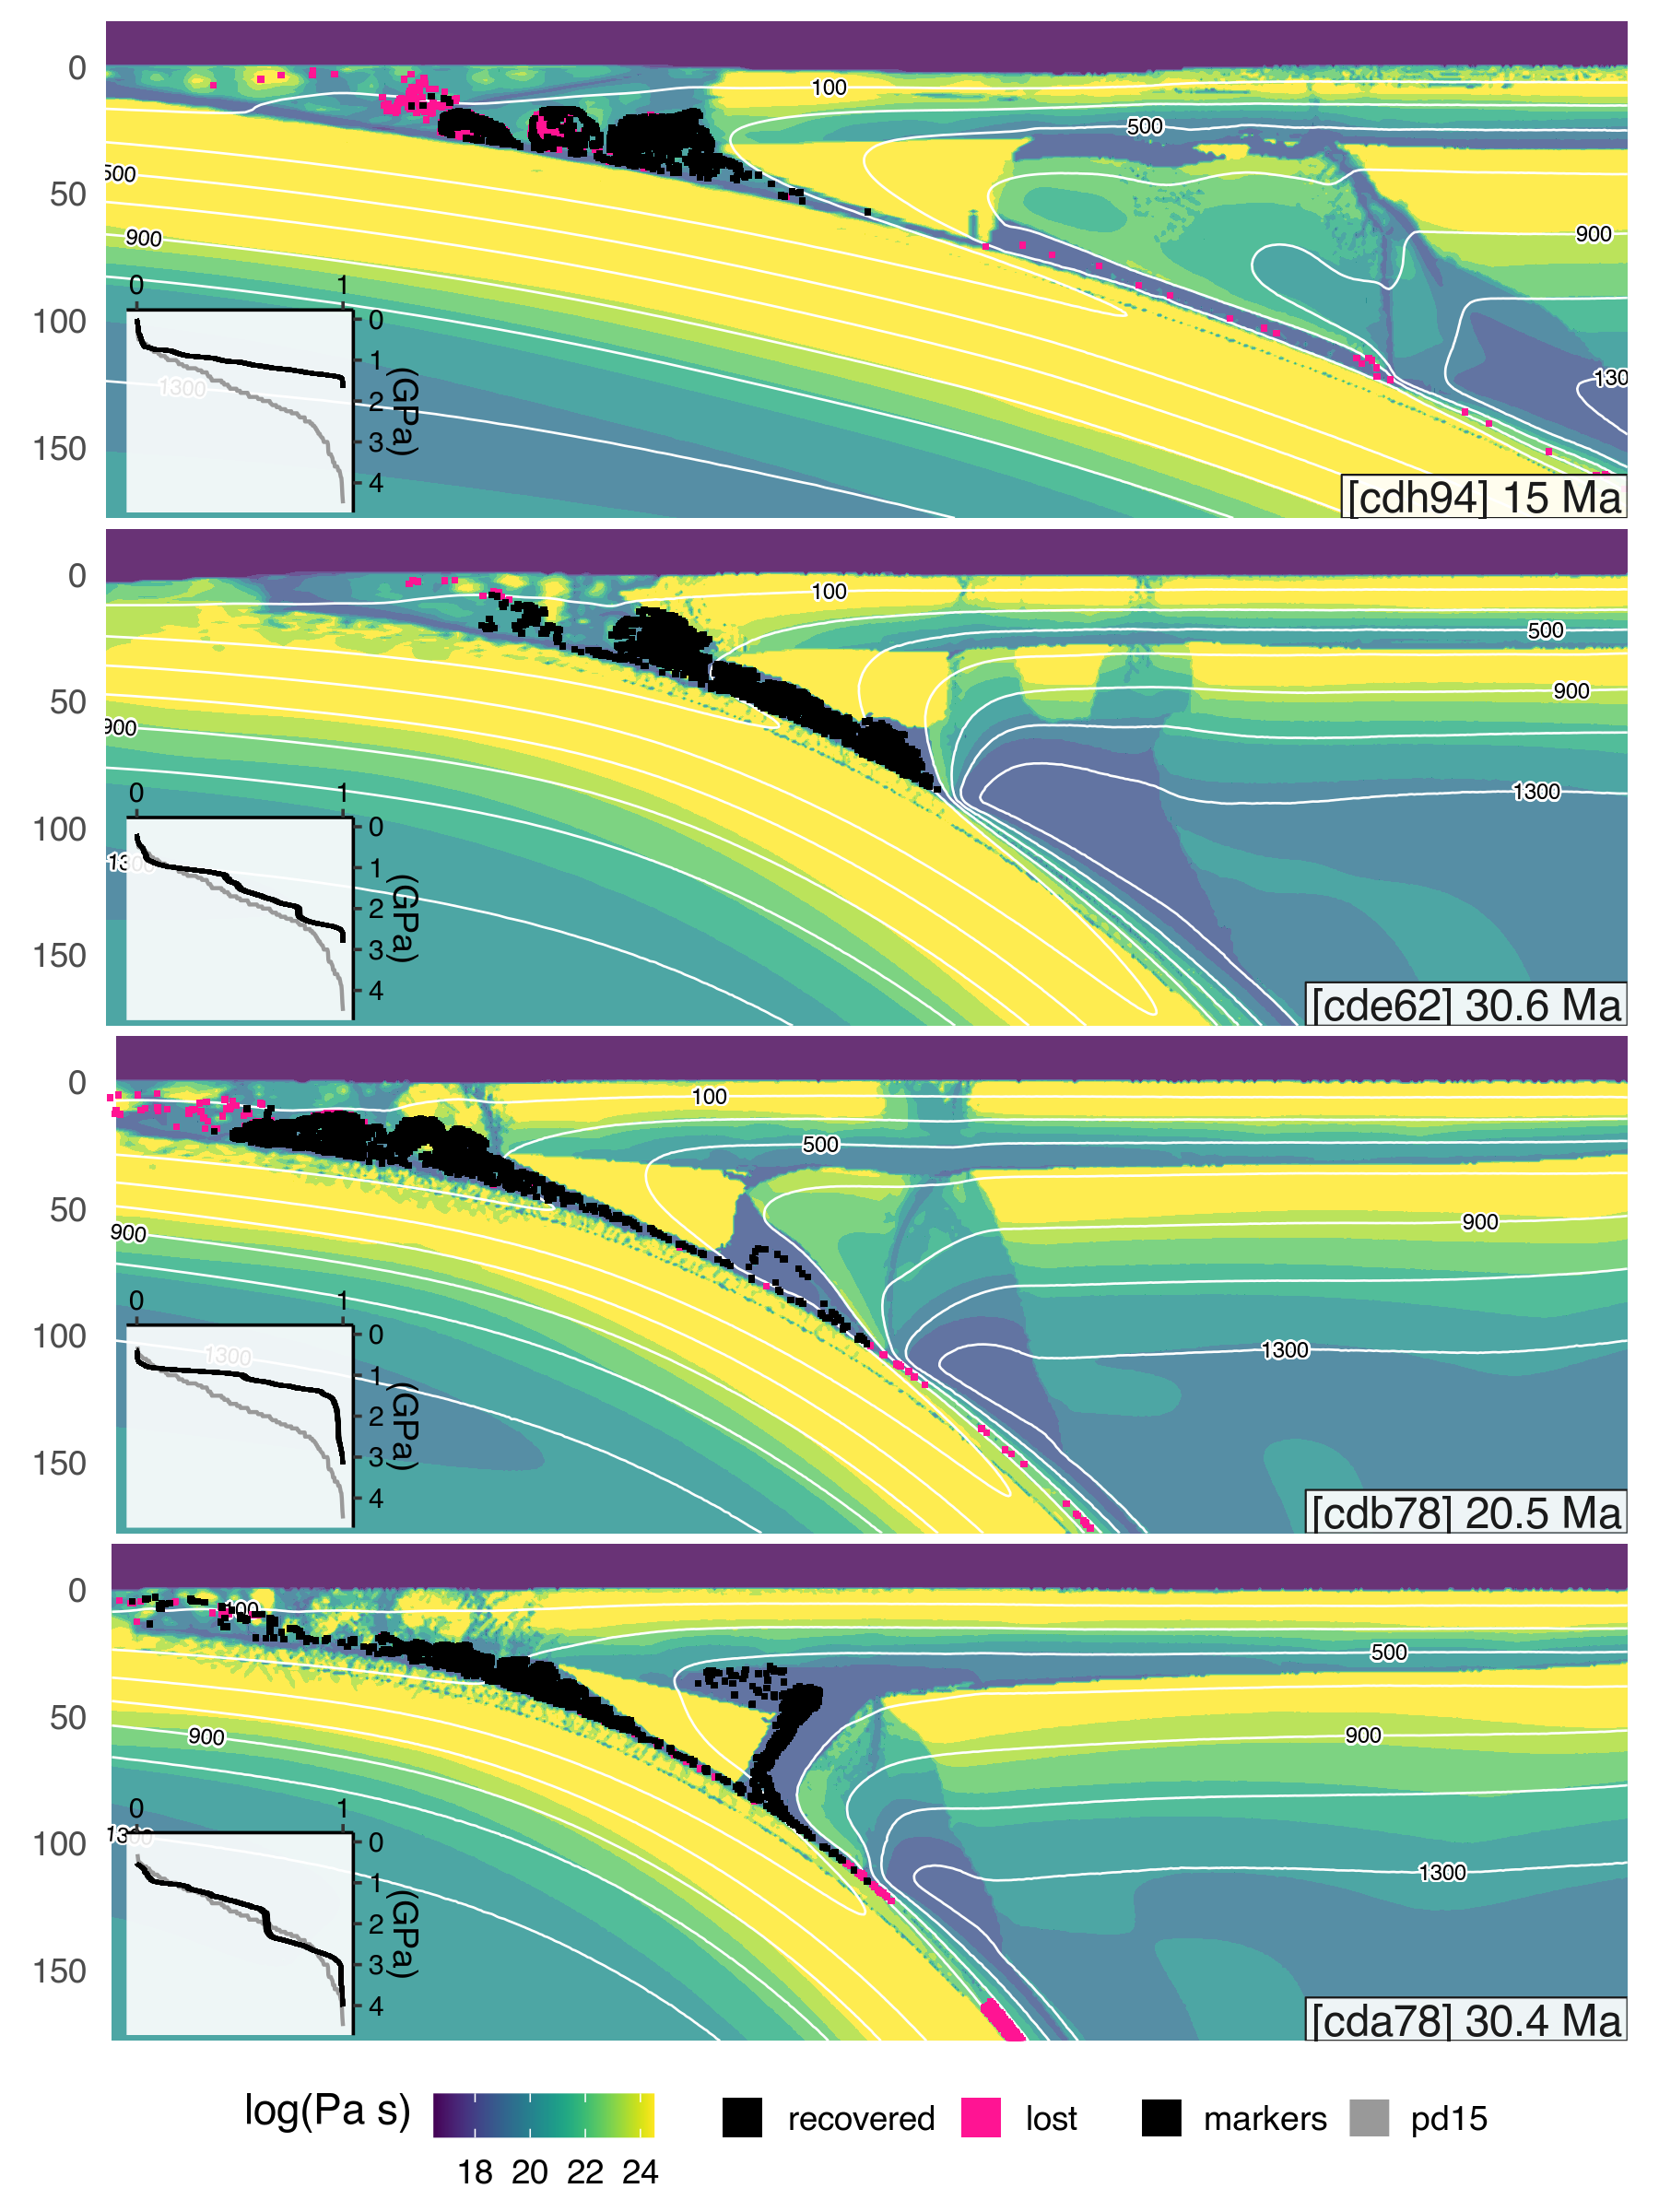
\includegraphics[width=0.85\linewidth,]{assets/figs/chpt4/geodynamics} 

}

\caption[Geodynamic regimes their probability distributions of recovered markers]{Geodynamic regimes generally observed in subduction simulations (main panels) and their marker \glspl{cdf} with respect to pressure (insets). Simulations with thick-rigid oceanic-plates (cdh94) tend to have low subduction angles, especially at high convergence rates (high-\(\Phi\)), and no eclogite recovery. The other three regimes all share flexible plates, higher subduction angles, and recovery of eclogites to different extents. Slowly-converging simulations (cde62) tend to have wide low-viscosity serpentinized channels that store underplated material uniformly with depth. Simulations like cde62 are consistent with \texttt{pd15} in terms of their \glspl{cdf} (inset). The final two regimes (cdb78 \& cda78) show deep opening of the serpentine channel. The mantle wedge completely detaches from the upper-plate in several models and diapirs rise in subvertical low-viscosity channels behind the mantle wedge. Simulations with diapirs also closely resemble \texttt{pd15} in terms their \glspl{cdf}.}\label{fig:geodyn}
\end{figure}

The other three geodynamic regimes share two commonalities: 1) they recover eclogites to various degrees, and 2) they have more flexible oceanic-plates and higher subduction angles. Slowly-converging systems with flexible plates (low-\(\Phi\)) tend to have wider subduction channels that accommodate more underplating of oceanic crust and sediments along the length of the subduction interface compared to flatter subduction angles (Figure \ref{fig:geodyn}, cde62). Markers from simulations with higher subduction angles display more uniform \glspl{cdf}, with respect to pressure, that closely resemble \texttt{pd15} (compare insets in Figure \ref{fig:geodyn}). These observations again imply rock recovery is sensitive to the geometry of subduction, which may be conflated with other thermo-kinematic boundary conditions when using \(\Phi\) as an explanatory variable.

The last two geodynamic regimes are characterized by narrow channels that widen at depth, separating the cold nose from the upper-plate (Figure \ref{fig:geodyn} cdb78, cda78). In many simulations, the mantle wedge separates entirely and the low-viscosity serpentine channel connects with the lower continental crust. A subvertical, low-viscosity corridor forms and markers rise as diapirs into the mantle wedge (Figure \ref{fig:geodyn}, cda78). Moreover, markers \glspl{cdf} from simulations with diapirs closely resemble \texttt{pd15} (compare insets in Figure \ref{fig:geodyn}). These simulations imply mantle wedge separation may be a plausible mechanism for diapir formation.

\hypertarget{chpt4Conclusions}{%
\section{Conclusion}\label{chpt4Conclusions}}

This study traces \gls{ptt} paths of more than one-million markers from 64 subduction simulations, identifies recovered markers, and computes their \gls{pt} distributions across a range of thermo-kinematic boundary conditions. \gls{ptt} distributions of recovered markers are compared with the rock record (\texttt{pd15}) to address the following hypotheses:

\begin{quote}
\begin{enumerate}
\def\labelenumi{\arabic{enumi}.}
\item
  The probability of recovering \gls{hp} rocks is relatively uniform up to 2.4 \(GPa\) (null: recovery is non-uniform with depth)
\item
  Recovery rates of \gls{hp} rocks vary with thermo-kinematic boundary conditions (null: recovery rates are not different among subduction zone)
\end{enumerate}
\end{quote}

With respect to the first hypothesis, \gls{pt} distributions of recovered markers are distinct from the rock record (\texttt{pd15}) across almost all simulations except for a minority of slowly-converging models (40 \(km/Ma\), Figure \ref{fig:ecdfs}), and models that develop separated mantle wedges and diapirs (Figure \ref{fig:geodyn}). The majority of simulations recovery relatively few markers from 0.8 to 2.4 \(GPa\) compared to \texttt{pd15}. This result implies \texttt{pd15} is overrepresented (biased) by \gls{hp} rocks between 0.8 and 2.4 \(GPa\). Differentiating the rock record by relevant metadata (lithology, metamorphic ages, thermo-kinematic boundary conditions estimates) is critically important to select against such bias (e.g., \protect\hyperlink{ref-agard2018}{Agard et al., 2018}).

With respect to the second hypothesis, recovered markers show a negative correlation between \(\Phi\) and recovery rate, implying a strong dependence of recovery rates on thermo-kinematic boundary conditions. However, simulations also show an apparent association between recovery rates and subduction angle. This may imply that recovery rates are sensitive to \(\Phi\) because of differences in subduction geometry, rather than oceanic-plate age or convergence velocity \emph{per se}. Correlations among recovery rate and thermo-kinematic boundary conditions are difficult to untangle because \(\Phi\) conflates thermo-kinematic effects (by design) and is therefore not the most precise explanatory variable. While a correlation between recovery rates and \(\Phi\) is apparent, the sensitivity of recovery rates to thermo-kinematic boundary conditions (Figure \ref{fig:recRate}), especially subduction geometry, warrants further investigation.

\cleardoublepage

\hypertarget{chpt5}{%
\chapter{Conclusion}\label{chpt5}}

\markboth{Chapter 5: Conclusion}{Chapter 5: Conclusion}

This work uses three computational approaches---simulation, interpolation, and applied statistics---to address the following question. How diverse is mechanical behavior along the plate interface across a range of plausible subduction zone configurations?

Plate coupling observed in numerical simulations from Chapter \ref{chpt2} demonstrate steady-state mechanical behavior regulated self-consistently by feedbacks involving heat transfer and metamorphic dehydration of ultramafic sheet silicates in the upper-plate mantle. Coupling depth is only weakly correlated with \(\Phi\) but strongly correlated with upper-plate lithospheric thickness. Thus uniform coupling depths are expected if subduction zones have uniformly thick upper-plates, which is indeed the case when considering averaged backarc surface heat flow for 17 presently active subduction zones (\protect\hyperlink{ref-currie2004}{Currie et al., 2004}; \protect\hyperlink{ref-currie2006}{Currie \& Hyndman, 2006}; \protect\hyperlink{ref-hyndman2005}{Hyndman et al., 2005}; \protect\hyperlink{ref-wada2009}{Wada \& Wang, 2009}).

However, 2D interpolations in Chapter \ref{chpt3} show diverse spatial patterns of surface heat flow---some implying homogeneous thermal structure, others implying heterogeneous thermal structure---near 13 presently active subduction zones. While Kriging methods yield inconsistent results for segments with low observational densities, Similarity methods show geologically-consistent interpolations of surface heat flow across all segments. Both methods, where applicable, generally agree and present surface heat flow interpolations in contradiction of broadly uniform upper-plate lithospheric thickness inferred from other (1D) sampling strategies (e.g., \protect\hyperlink{ref-currie2004}{Currie et al., 2004}; \protect\hyperlink{ref-currie2006}{Currie \& Hyndman, 2006}; \protect\hyperlink{ref-hyndman2005}{Hyndman et al., 2005}; \protect\hyperlink{ref-wada2009}{Wada \& Wang, 2009}). These results imply broadly non-uniform coupling depths among subduction zones.

Chapter \ref{chpt4} takes a different approach by considering what \gls{pt} distributions of \gls{hp} rocks imply about mechanical variability among subduction zones. A large (91,733) dataset of recovered markers shows marker \gls{ptt} distributions and recovery rates correlate with \(\Phi\) and subduction duration, but not upper-plate lithospheric thickness (as expected from Chapter \ref{chpt2}). These results imply broad differences in the mechanics of rock recovery through time and among subduction zones.

While self-regulating mechanisms of uniform (and sustained) depths of plate coupling among different subduction zones are plausible (Chapter \ref{chpt2}), 2D interpolations of surface heat flow (Chapter \ref{chpt3}), and \gls{ptt} distributions of recovered markers (Chapter \ref{chpt4}) imply a more diverse picture of mechanical behavior across different subduction zone settings. One reason for such assorted conclusions is using a relatively crude explanatory variable (\(\Phi\)) for comparison. \(\Phi\) is demonstrably useful for explaining variability among some features of subduction geodynamics (\protect\hyperlink{ref-gorbatov1997}{Gorbatov \& Kostoglodov, 1997}; \protect\hyperlink{ref-kirby1991}{Kirby et al., 1991}; \protect\hyperlink{ref-molnar1979}{Molnar et al., 1979}; \protect\hyperlink{ref-syracuse2010}{Syracuse et al., 2010}; \protect\hyperlink{ref-wada2009}{Wada \& Wang, 2009}), but demonstrably ineffective in many cases (\protect\hyperlink{ref-maunder2019}{Maunder et al., 2019}). Future work may focus on developing new explanatory variables, scaling surface heat flow datasets, and developing composite interpolation approaches to better estimate relative geodynamic variability among subduction zones.

\cleardoublepage

\hypertarget{references}{%
\chapter*{References}\label{references}}
\addcontentsline{toc}{chapter}{References}

\markboth{References}{References}

\hypertarget{refs_main}{}
\begin{CSLReferences}{1}{1}
\leavevmode\vadjust pre{\hypertarget{ref-abers2017}{}}%
Abers, G., van Keken, P., \& Hacker, B. (2017). The cold and relatively dry nature of mantle forearcs in subduction zones. \emph{Nature Geoscience}, \emph{10}(5), 333--337.

\leavevmode\vadjust pre{\hypertarget{ref-afonso2005}{}}%
Afonso, J. C., Ranalli, G., \& Fernàndez, M. (2005). Thermal expansivity and elastic properties of the lithospheric mantle: Results from mineral physics of composites. \emph{Physics of the Earth and Planetary Interiors}, \emph{149}(3-4), 279--306.

\leavevmode\vadjust pre{\hypertarget{ref-agard2009}{}}%
Agard, P., Yamato, P., Jolivet, L., \& Burov, E. (2009). Exhumation of oceanic blueschists and eclogites in subduction zones: Timing and mechanisms. \emph{Earth-Science Reviews}, \emph{92}(1-2), 53--79.

\leavevmode\vadjust pre{\hypertarget{ref-agard2016}{}}%
Agard, P., Yamato, P., Soret, M., Prigent, C., Guillot, S., Plunder, A., et al. (2016). Plate interface rheological switches during subduction infancy: Control on slab penetration and metamorphic sole formation. \emph{Earth and Planetary Science Letters}, \emph{451}, 208--220.

\leavevmode\vadjust pre{\hypertarget{ref-agard2018}{}}%
Agard, P., Plunder, A., Angiboust, S., Bonnet, G., \& Ruh, J. (2018). The subduction plate interface: Rock record and mechanical coupling (from long to short time scales). \emph{Lithos}, \emph{320-321}, 537--566.

\leavevmode\vadjust pre{\hypertarget{ref-agrusta2013}{}}%
Agrusta, R., Arcay, D., Tommasi, A., Davaille, A., Ribe, N., \& Gerya, T. (2013). Small-scale convection in a plume-fed low-viscosity layer beneath a moving plate. \emph{Geophysical Journal International}, \emph{194}(2), 591--610.

\leavevmode\vadjust pre{\hypertarget{ref-angiboust2012a}{}}%
Angiboust, S., Langdon, R., Agard, P., Waters, D., \& Chopin, C. (2012a). Eclogitization of the monviso ophiolite (w. Alps) and implications on subduction dynamics. \emph{Journal of Metamorphic Geology}, \emph{30}(1), 37--61.

\leavevmode\vadjust pre{\hypertarget{ref-angiboust2012b}{}}%
Angiboust, S., Wolf, S., Burov, E., Agard, P., \& Yamato, P. (2012b). Effect of fluid circulation on subduction interface tectonic processes: Insights from thermo-mechanical numerical modelling. \emph{Earth and Planetary Science Letters}, \emph{357}, 238--248.

\leavevmode\vadjust pre{\hypertarget{ref-angiboust2014}{}}%
Angiboust, S., Pettke, T., De Hoog, J., Caron, B., \& Oncken, O. (2014). Channelized fluid flow and eclogite-facies metasomatism along the subduction shear zone. \emph{Journal of Petrology}, \emph{55}(5), 883--916.

\leavevmode\vadjust pre{\hypertarget{ref-arcay2006}{}}%
Arcay, D., Doin, M., Tric, E., Bousquet, R., \& de Capitani, C. (2006). Overriding plate thinning in subduction zones: Localized convection induced by slab dehydration. \emph{Geochemistry, Geophysics, Geosystems}, \emph{7}(2).

\leavevmode\vadjust pre{\hypertarget{ref-arcay2007}{}}%
Arcay, D., Tric, E., \& Doin, M. (2007). Slab surface temperature in subduction zones: Influence of the interplate decoupling depth and upper plate thinning processes. \emph{Earth and Planetary Science Letters}, \emph{255}(3-4), 324--338.

\leavevmode\vadjust pre{\hypertarget{ref-archinal2018}{}}%
Archinal, B., Acton, C., A'hearn, M., Conrad, A., Consolmagno, G., Duxbury, T., et al. (2018). Report of the IAU working group on cartographic coordinates and rotational elements: 2015. \emph{Celestial Mechanics and Dynamical Astronomy}, \emph{130}(3), 1--46.

\leavevmode\vadjust pre{\hypertarget{ref-banfield1993}{}}%
Banfield, J. D., \& Raftery, A. E. (1993). Model-based gaussian and non-gaussian clustering. \emph{Biometrics}, 803--821.

\leavevmode\vadjust pre{\hypertarget{ref-bardossy1997}{}}%
Bárdossy, A. (1997). Introduction to geostatistics. \emph{Institute of Hydraulic Engineering, University of Stuttgart}.

\leavevmode\vadjust pre{\hypertarget{ref-barlow1989}{}}%
Barlow, H. B. (1989). Unsupervised learning. \emph{Neural Computation}, \emph{1}(3), 295--311.

\leavevmode\vadjust pre{\hypertarget{ref-batchelor1953}{}}%
Batchelor, G. K. (1953). \emph{The theory of homogeneous turbulence}. Cambridge university press.

\leavevmode\vadjust pre{\hypertarget{ref-bebout2007}{}}%
Bebout, G. E. (2007). Metamorphic chemical geodynamics of subduction zones. \emph{Earth and Planetary Science Letters}, \emph{260}(3-4), 373--393.

\leavevmode\vadjust pre{\hypertarget{ref-bebout2002}{}}%
Bebout, G. E., \& Barton, M. D. (2002). Tectonic and metasomatic mixing in a high-t, subduction-zone m{é}lange---insights into the geochemical evolution of the slab--mantle interface. \emph{Chemical Geology}, \emph{187}(1-2), 79--106.

\leavevmode\vadjust pre{\hypertarget{ref-bird2003}{}}%
Bird, P. (2003). An updated digital model of plate boundaries. \emph{Geochemistry, Geophysics, Geosystems}, \emph{4}(3).

\leavevmode\vadjust pre{\hypertarget{ref-bittner1995}{}}%
Bittner, D., \& Schmeling, H. (1995). Numerical modelling of melting processes and induced diapirism in the lower crust. \emph{Geophysical Journal International}, \emph{123}(1), 59--70.

\leavevmode\vadjust pre{\hypertarget{ref-boussinesq1897}{}}%
Boussinesq, J. (1897). \emph{Th{é}orie de l'{é}coulement tourbillonnant et tumultueux des liquides dans les lits rectilignes a grande section} (Vol. 1). Gauthier-Villars.

\leavevmode\vadjust pre{\hypertarget{ref-burg2005}{}}%
Burg, J., \& Gerya, T. (2005). The role of viscous heating in barrovian metamorphism of collisional orogens: Thermomechanical models and application to the lepontine dome in the central alps. \emph{Journal of Metamorphic Geology}, \emph{23}(2), 75--95.

\leavevmode\vadjust pre{\hypertarget{ref-burov2001}{}}%
Burov, E., Jolivet, L., Le Pourhiet, L., \& Poliakov, A. (2001). A thermomechanical model of exhumation of high pressure (HP) and ultra-high pressure (UHP) metamorphic rocks in alpine-type collision belts. \emph{Tectonophysics}, \emph{342}(1-2), 113--136.

\leavevmode\vadjust pre{\hypertarget{ref-burov2014}{}}%
Burov, E., François, T., Agard, P., Le Pourhiet, L., Meyer, B., Tirel, C., et al. (2014). Rheological and geodynamic controls on the mechanisms of subduction and HP/UHP exhumation of crustal rocks during continental collision: Insights from numerical models. \emph{Tectonophysics}, \emph{631}, 212--250.

\leavevmode\vadjust pre{\hypertarget{ref-byerlee1978}{}}%
Byerlee, J. (1978). Friction of rocks. In \emph{Rock friction and earthquake prediction} (Vol. 116, pp. 615--626). Birkh{ä}user Basel.

\leavevmode\vadjust pre{\hypertarget{ref-byrne2020}{}}%
Byrne, K. A. (2020). Borah: Dell HPC intel (high performance computing cluster).

\leavevmode\vadjust pre{\hypertarget{ref-carlson2003}{}}%
Carlson, R., \& Miller, D. (2003). Mantle wedge water contents estimated from seismic velocities in partially serpentinized peridotites. \emph{Geophysical Research Letters}, \emph{30}(5).

\leavevmode\vadjust pre{\hypertarget{ref-celeux1995}{}}%
Celeux, G., \& Govaert, G. (1995). Gaussian parsimonious clustering models. \emph{Pattern Recognition}, \emph{28}(5), 781--793.

\leavevmode\vadjust pre{\hypertarget{ref-chapman1975}{}}%
Chapman, D., \& Pollack, H. (1975). Global heat flow: A new look. \emph{Earth and Planetary Science Letters}, \emph{28}(1), 23--32.

\leavevmode\vadjust pre{\hypertarget{ref-chiles2009}{}}%
Chiles, J. P., \& Delfiner, P. (2009). \emph{Geostatistics: Modeling spatial uncertainty} (Vol. 497). John Wiley \& Sons.

\leavevmode\vadjust pre{\hypertarget{ref-cizkova2013}{}}%
Čížková, H., \& Bina, C. (2013). Effects of mantle and subduction-interface rheologies on slab stagnation and trench rollback. \emph{Earth and Planetary Science Letters}, \emph{379}, 95--103.

\leavevmode\vadjust pre{\hypertarget{ref-clauser1995}{}}%
Clauser, C., \& Huenges, E. (1995). Thermal conductivity of rocks and minerals. \emph{Rock Physics and Phase Relations: A Handbook of Physical Constants}, \emph{3}, 105--126.

\leavevmode\vadjust pre{\hypertarget{ref-cleveland1988}{}}%
Cleveland, W. S., \& Devlin, S. J. (1988). Locally weighted regression: An approach to regression analysis by local fitting. \emph{Journal of the American Statistical Association}, \emph{83}(403), 596--610.

\leavevmode\vadjust pre{\hypertarget{ref-coffin1997}{}}%
Coffin, M., Gahagan, L., \& Lawver, L. (1997). \emph{Present-day plate boundary digital data compilation}. Institute for Geophysics.

\leavevmode\vadjust pre{\hypertarget{ref-connolly2005}{}}%
Connolly, J. (2005). Computation of phase equilibria by linear programming: A tool for geodynamic modeling and its application to subduction zone decarbonation. \emph{Earth and Planetary Science Letters}, \emph{236}(1-2), 524--541.

\leavevmode\vadjust pre{\hypertarget{ref-cressie2015}{}}%
Cressie, N. (2015). \emph{Statistics for spatial data}. John Wiley \& Sons.

\leavevmode\vadjust pre{\hypertarget{ref-currie2006}{}}%
Currie, C., \& Hyndman, R. (2006). The thermal structure of subduction zone back arcs. \emph{Journal of Geophysical Research: Solid Earth}, \emph{111}(B8), 1--22.

\leavevmode\vadjust pre{\hypertarget{ref-currie2004}{}}%
Currie, C., Wang, K., Hyndman, R., \& He, J. (2004). The thermal effects of steady-state slab-driven mantle flow above a subducting plate: The cascadia subduction zone and backarc. \emph{Earth and Planetary Science Letters}, \emph{223}(1-2), 35--48.

\leavevmode\vadjust pre{\hypertarget{ref-davies1999}{}}%
Davies, J. (1999). The role of hydraulic fractures and intermediate depth earthquakes in generating suduction zone magmatism. \emph{Nature}, \emph{417}(March), 142--145.

\leavevmode\vadjust pre{\hypertarget{ref-davies2013}{}}%
Davies, J. (2013). Global map of solid earth surface heat flow. \emph{Geochemistry, Geophysics, Geosystems}, \emph{14}(10), 4608--4622.

\leavevmode\vadjust pre{\hypertarget{ref-dempster1977}{}}%
Dempster, A. P., Laird, N. M., \& Rubin, D. B. (1977). Maximum likelihood from incomplete data via the EM algorithm. \emph{Journal of the Royal Statistical Society: Series B (Methodological)}, \emph{39}(1), 1--22.

\leavevmode\vadjust pre{\hypertarget{ref-dy2004}{}}%
Dy, J. G., \& Brodley, C. E. (2004). Feature selection for unsupervised learning. \emph{Journal of Machine Learning Research}, \emph{5}(Aug), 845--889.

\leavevmode\vadjust pre{\hypertarget{ref-efron1992}{}}%
Efron, B. (1992). Bootstrap methods: Another look at the jackknife. In \emph{Breakthroughs in statistics} (pp. 569--593). Springer.

\leavevmode\vadjust pre{\hypertarget{ref-efron1994}{}}%
Efron, B., \& Tibshirani, R. J. (1994). \emph{An introduction to the bootstrap}. CRC press.

\leavevmode\vadjust pre{\hypertarget{ref-engdahl1998}{}}%
Engdahl, E., van der Hilst, R., \& Buland, R. (1998). Global teleseismic earthquake relocation with improved travel times and procedures for depth determination. \emph{Bulletin of the Seismological Society of America}, \emph{88}(3), 722--743.

\leavevmode\vadjust pre{\hypertarget{ref-england2010}{}}%
England, P., \& Katz, R. (2010). Melting above the anhydrous solidus controls the location of volcanic arcs. \emph{Nature}, \emph{467}(7316), 700--703.

\leavevmode\vadjust pre{\hypertarget{ref-england2004}{}}%
England, P., Engdahl, R., \& Thatcher, W. (2004). Systematic variation in the depths of slabs beneath arc volcanoes. \emph{Geophysical Journal International}, \emph{156}(2), 377--408.

\leavevmode\vadjust pre{\hypertarget{ref-faccenda2009}{}}%
Faccenda, M., Gerya, T., \& Burlini, L. (2009). Deep slab hydration induced by bending-related variations in tectonic pressure. \emph{Nature Geoscience}, \emph{2}(11), 790--793.

\leavevmode\vadjust pre{\hypertarget{ref-ferris2003}{}}%
Ferris, A., Abers, G. A., Christensen, D. H., \& Veenstra, E. (2003). High resolution image of the subducted pacific (?) Plate beneath central alaska, 50--150 km depth. \emph{Earth and Planetary Science Letters}, \emph{214}(3-4), 575--588.

\leavevmode\vadjust pre{\hypertarget{ref-figueiredo2002}{}}%
Figueiredo, M. A. T., \& Jain, A. K. (2002). Unsupervised learning of finite mixture models. \emph{IEEE Transactions on Pattern Analysis and Machine Intelligence}, \emph{24}(3), 381--396.

\leavevmode\vadjust pre{\hypertarget{ref-fourier1827}{}}%
Fourier, J. (1827). Mémoire sur les températures du globe terrestre et des espaces planétaires. \emph{Mémoires de l'Académie Royale Des Sciences de l'Institut de France}, \emph{7}, 570--604.

\leavevmode\vadjust pre{\hypertarget{ref-fraley2002}{}}%
Fraley, C., \& Raftery, A. E. (2002). Model-based clustering, discriminant analysis, and density estimation. \emph{Journal of the American Statistical Association}, \emph{97}(458), 611--631.

\leavevmode\vadjust pre{\hypertarget{ref-furlong2013}{}}%
Furlong, K., \& Chapman, D. (2013). Heat flow, heat generation, and the thermal state of the lithosphere. \emph{Annual Review of Earth and Planetary Sciences}, \emph{41}(1), 385--410.

\leavevmode\vadjust pre{\hypertarget{ref-furukawa1993}{}}%
Furukawa, Y. (1993). Depth of the decoupling plate interface and thermal structure under arcs. \emph{Journal of Geophysical Research: Solid Earth}, \emph{98}(B11), 20005--20013.

\leavevmode\vadjust pre{\hypertarget{ref-gao2014}{}}%
Gao, X., \& Wang, K. (2014). Strength of stick-slip and creeping subduction megathrusts from heat flow observations. \emph{Science}, \emph{345}(6200), 1038--1041.

\leavevmode\vadjust pre{\hypertarget{ref-gao2017}{}}%
Gao, X., \& Wang, K. (2017). Rheological separation of the megathrust seismogenic zone and episodic tremor and slip. \emph{Nature}, \emph{543}(7645), 416--419.

\leavevmode\vadjust pre{\hypertarget{ref-gerya2014}{}}%
Gerya, T. (2014). Precambrian geodynamics: Concepts and models. \emph{Gondwana Research}, \emph{25}(2), 442--463.

\leavevmode\vadjust pre{\hypertarget{ref-gerya2011}{}}%
Gerya, T., \& Meilick, F. (2011). Geodynamic regimes of subduction under an active margin: Effects of rheological weakening by fluids and melts. \emph{Journal of Metamorphic Geology}, \emph{29}(1), 7--31.

\leavevmode\vadjust pre{\hypertarget{ref-gerya2003}{}}%
Gerya, T., \& Yuen, D. (2003). Characteristics-based marker-in-cell method with conservative finite-differences schemes for modeling geological flows with strongly variable transport properties. \emph{Physics of the Earth and Planetary Interiors}, \emph{140}(4), 293--318.

\leavevmode\vadjust pre{\hypertarget{ref-gerya2008}{}}%
Gerya, T., Connolly, J., \& Yuen, D. (2008). Why is terrestrial subduction one-sided? \emph{Geology}, \emph{36}(1), 43--46.

\leavevmode\vadjust pre{\hypertarget{ref-gerya2019}{}}%
Gerya, T. V. (2019). \emph{Introduction to numerical geodynamic modelling}. Cambridge University Press.

\leavevmode\vadjust pre{\hypertarget{ref-gerya2006}{}}%
Gerya, T. V., \& Stöckhert, B. (2006). Two-dimensional numerical modeling of tectonic and metamorphic histories at active continental margins. \emph{International Journal of Earth Sciences}, \emph{95}(2), 250--274.

\leavevmode\vadjust pre{\hypertarget{ref-gerya2002}{}}%
Gerya, T. V., Stöckhert, B., \& Perchuk, A. L. (2002). Exhumation of high-pressure metamorphic rocks in a subduction channel: A numerical simulation. \emph{Tectonics}, \emph{21}(6), 6--1.

\leavevmode\vadjust pre{\hypertarget{ref-goldberg1989}{}}%
Goldberg, D. (1989). Genetic algorithms in search. \emph{Optimization, and MachineLearning}.

\leavevmode\vadjust pre{\hypertarget{ref-gonzalez2016}{}}%
Gonzalez, C., Gorczyk, W., \& Gerya, T. (2016). Decarbonation of subducting slabs: Insight from petrological--thermomechanical modeling. \emph{Gondwana Research}, \emph{36}, 314--332.

\leavevmode\vadjust pre{\hypertarget{ref-goodchild2004}{}}%
Goodchild, M. (2004). The validity and usefulness of laws in geographic information science and geography. \emph{Annals of the Association of American Geographers}, \emph{94}(2), 300--303.

\leavevmode\vadjust pre{\hypertarget{ref-goovaerts1997}{}}%
Goovaerts, P. (1997). \emph{Geostatistics for natural resources evaluation}. Oxford University Press on Demand.

\leavevmode\vadjust pre{\hypertarget{ref-gorbatov1997}{}}%
Gorbatov, A., \& Kostoglodov, V. (1997). Maximum depth of seismicity and thermal parameter of the subducting slab: General empirical relation and its application. \emph{Tectonophysics}, \emph{277}(1-3), 165--187.

\leavevmode\vadjust pre{\hypertarget{ref-gorczyk2007}{}}%
Gorczyk, W., Willner, A., Gerya, T., Connolly, J., \& Burg, J. (2007). Physical controls of magmatic productivity at pacific-type convergent margins: Numerical modelling. \emph{Physics of the Earth and Planetary Interiors}, \emph{163}(1-4), 209--232.

\leavevmode\vadjust pre{\hypertarget{ref-goutorbe2011}{}}%
Goutorbe, B., Poort, J., Lucazeau, F., \& Raillard, S. (2011). Global heat flow trends resolved from multiple geological and geophysical proxies. \emph{Geophysical Journal International}, \emph{187}(3), 1405--1419.

\leavevmode\vadjust pre{\hypertarget{ref-graler2016}{}}%
Gräler, B., Pebesma, E., \& Heuvelink, G. (2016). Spatio-temporal interpolation using gstat. \emph{The R Journal}, \emph{8}, 204--218. Retrieved from \url{https://journal.r-project.org/archive/2016/RJ-2016-014/index.html}

\leavevmode\vadjust pre{\hypertarget{ref-grove2009}{}}%
Grove, T., Till, C., Lev, E., Chatterjee, N., \& Médard, E. (2009). Kinematic variables and water transport control the formation and location of arc volcanoes. \emph{Nature}, \emph{459}(7247), 694--697.

\leavevmode\vadjust pre{\hypertarget{ref-grove2012}{}}%
Grove, T., Till, C., \& Krawczynski, M. (2012). The role of \(H_2O\) in subduction zone magmatism. \emph{Annual Review of Earth and Planetary Sciences}, \emph{40}(1), 413--439.

\leavevmode\vadjust pre{\hypertarget{ref-hacker2003}{}}%
Hacker, B., Abers, G., \& Peacock, S. (2003). Subduction factory 1. Theoretical mineralogy, densities, seismic wave speeds, and \(H_2O\) contents. \emph{Journal of Geophysical Research: Solid Earth}, \emph{108}(B1).

\leavevmode\vadjust pre{\hypertarget{ref-harlow1962}{}}%
Harlow, F. (1962). \emph{The particle-in-cell method for numerical solution of problems in fluid dynamics}. Los Alamos Scientific Lab., N. Mex.

\leavevmode\vadjust pre{\hypertarget{ref-harlow1964}{}}%
Harlow, F. (1964). The particle-in-cell computing method for fluid dynamics. \emph{Methods Comput. Phys.}, \emph{3}, 319--343.

\leavevmode\vadjust pre{\hypertarget{ref-harlow1965}{}}%
Harlow, F. H., \& Welch, J. E. (1965). Numerical calculation of time-dependent viscous incompressible flow of fluid with free surface. \emph{The Physics of Fluids}, \emph{8}(12), 2182--2189.

\leavevmode\vadjust pre{\hypertarget{ref-hasterok2013}{}}%
Hasterok, D. (2013). A heat flow based cooling model for tectonic plates. \emph{Earth and Planetary Science Letters}, \emph{361}, 34--43.

\leavevmode\vadjust pre{\hypertarget{ref-hasterok2008}{}}%
Hasterok, D., \& Chapman, D. (2008). Global heat flow: A new database and a new approach. In \emph{AGU fall meeting abstracts} (Vol. 2008, pp. T21c--1985).

\leavevmode\vadjust pre{\hypertarget{ref-hasterok2011}{}}%
Hasterok, D., Chapman, D., \& Davis, E. (2011). Oceanic heat flow: Implications for global heat loss. \emph{Earth and Planetary Science Letters}, \emph{311}(3-4), 386--395.

\leavevmode\vadjust pre{\hypertarget{ref-hilairet2007}{}}%
Hilairet, N., Reynard, B., Wang, Y., Daniel, I., Merkel, S., Nishiyama, N., \& Petitgirard, S. (2007). High-pressure creep of serpentine, interseismic deformation, and initiation of subduction. \emph{Science}, \emph{318}(5858), 1910--1913.

\leavevmode\vadjust pre{\hypertarget{ref-hirauchi2010}{}}%
Hirauchi, K., Katayama, I., Uehara, S., Miyahara, M., \& Takai, Y. (2010). Inhibition of subduction thrust earthquakes by low-temperature plastic flow in serpentine. \emph{Earth and Planetary Science Letters}, \emph{295}(3-4), 349--357.

\leavevmode\vadjust pre{\hypertarget{ref-holt2021}{}}%
Holt, A. F., \& Condit, C. B. (2021). Slab temperature evolution over the lifetime of a subduction zone. \emph{Geochemistry, Geophysics, Geosystems}, e2020GC009476.

\leavevmode\vadjust pre{\hypertarget{ref-hu2020}{}}%
Hu, J., \& Gurnis, M. (2020). Subduction duration and slab dip. \emph{Geochemistry, Geophysics, Geosystems}, \emph{21}(4), e2019GC008862.

\leavevmode\vadjust pre{\hypertarget{ref-hyndman2003}{}}%
Hyndman, R., \& Peacock, S. (2003). Serpentinization of the forearc mantle. \emph{Earth and Planetary Science Letters}, \emph{212}(3-4), 417--432.

\leavevmode\vadjust pre{\hypertarget{ref-hyndman2005}{}}%
Hyndman, R., Currie, C., \& Mazzotti, S. (2005). Subduction zone backarcs, mobile belts, and orogenic heat. \emph{GSA Today}, \emph{15}(2), 4--10.

\leavevmode\vadjust pre{\hypertarget{ref-ito1971}{}}%
Ito, K., \& Kennedy, G. (1971). An experimental study of the basalt-garnet granulite-eclogite transition. \emph{The Structure and Physical Properties of the Earth's Crust}, \emph{14}, 303--314.

\leavevmode\vadjust pre{\hypertarget{ref-jennings2021}{}}%
Jennings, S., \& Hasterok, D. (2021). HeatFlow.org. \emph{Heatflow.org}. Retrieved from \url{http://heatflow.org/}

\leavevmode\vadjust pre{\hypertarget{ref-jull2001}{}}%
Jull, M., \& Kelemen, P. (2001). On the conditions for lower crustal convective instability. \emph{Journal of Geophysical Research: Solid Earth}, \emph{106}(b4), 6423--6446.

\leavevmode\vadjust pre{\hypertarget{ref-karato1993}{}}%
Karato, S., \& Wu, P. (1993). Rheology of the upper mantle: A synthesis. \emph{Science}, \emph{260}(5109), 771--778.

\leavevmode\vadjust pre{\hypertarget{ref-kelvin1863}{}}%
Kelvin, W. T. (1863). On the secular cooling of the earth. \emph{Transactions of the Royal Society of Edinburgh}, \emph{23}, 157--170.

\leavevmode\vadjust pre{\hypertarget{ref-kerswell2020}{}}%
Kerswell, B., Kohn, M., \& Gerya, T. (2020). Backarc lithospheric thickness and serpentine stability control slab-mantle coupling depths in subduction zones. \emph{Geochemistry, Geophysics, Geosystems}, e2020GC009304.

\leavevmode\vadjust pre{\hypertarget{ref-kerswell2021}{}}%
Kerswell, B. C., \& Kohn, M. J. (2021). \emph{A comparison of heat flow interpolations near subduction zones}.

\leavevmode\vadjust pre{\hypertarget{ref-kirby1991}{}}%
Kirby, S. H., Durham, W. B., \& Stern, L. A. (1991). Mantle phase changes and deep-earthquake faulting in subducting lithosphere. \emph{Science}, \emph{252}(5003), 216--225.

\leavevmode\vadjust pre{\hypertarget{ref-kohavi1995}{}}%
Kohavi, R. (1995). A study of cross-validation and bootstrap for accuracy estimation and model selection. In \emph{Ijcai} (Vol. 14, pp. 1137--1145). Montreal, Canada.

\leavevmode\vadjust pre{\hypertarget{ref-kohn2018}{}}%
Kohn, M. J., Castro, A. E., Kerswell, B. C., Ranero, C. R., \& Spear, F. S. (2018). Shear heating reconciles thermal models with the metamorphic rock record of subduction. \emph{Proceedings of the National Academy of Sciences}, \emph{115}(46), 11706--11711.

\leavevmode\vadjust pre{\hypertarget{ref-krige1951}{}}%
Krige, D. (1951). A statistical approach to some basic mine valuation problems on the witwatersrand. \emph{Journal of the Southern African Institute of Mining and Metallurgy}, \emph{52}(6), 119--139.

\leavevmode\vadjust pre{\hypertarget{ref-lawver2018}{}}%
Lawver, L. A., Dalziel, I. W., Norton, I. O., Gahagan, L., \& Davis, J. (2018). The PLATES 2014 atlas of plate reconstructions (550 ma to present day), PLATES progress report no. 374-0215. \emph{University of Texas Institute for Geophysics Technical Reports}.

\leavevmode\vadjust pre{\hypertarget{ref-lee1965}{}}%
Lee, W., \& Uyeda, S. (1965). Review of heat flow data. \emph{Terrestrial Heat Flow}, \emph{8}, 87--190.

\leavevmode\vadjust pre{\hypertarget{ref-li2018}{}}%
Li, Z., Zhang, X., Clarke, K., Liu, G., \& Zhu, R. (2018). An automatic variogram modeling method with high reliability fitness and estimates. \emph{Computers \& Geosciences}, \emph{120}, 48--59.

\leavevmode\vadjust pre{\hypertarget{ref-lucazeau2019}{}}%
Lucazeau, F. (2019). Analysis and mapping of an updated terrestrial heat flow data set. \emph{Geochemistry, Geophysics, Geosystems}, \emph{20}(8), 4001--4024.

\leavevmode\vadjust pre{\hypertarget{ref-matheron1963}{}}%
Matheron, G. (1963). Principles of geostatistics. \emph{Economic Geology}, \emph{58}(8), 1246--1266.

\leavevmode\vadjust pre{\hypertarget{ref-matheron2019}{}}%
Matheron, G. (2019). \emph{Matheron's theory of regionalized variables}. International Association for.

\leavevmode\vadjust pre{\hypertarget{ref-maunder2019}{}}%
Maunder, B., Hunen, J. van, Bouilhol, P., \& Magni, V. (2019). Modeling slab temperature: A reevaluation of the thermal parameter. \emph{Geochemistry, Geophysics, Geosystems}, \emph{20}(2), 673--687.

\leavevmode\vadjust pre{\hypertarget{ref-mckenzie1969}{}}%
McKenzie, D. (1969). Speculations on the consequences and causes of plate motions. \emph{Geophysical Journal International}, \emph{18}(1), 1--32.

\leavevmode\vadjust pre{\hypertarget{ref-molnar1979}{}}%
Molnar, P., Freedman, D., \& Shih, J. S. (1979). Lengths of intermediate and deep seismic zones and temperatures in downgoing slabs of lithosphere. \emph{Geophysical Journal International}, \emph{56}(1), 41--54.

\leavevmode\vadjust pre{\hypertarget{ref-moresi2003}{}}%
Moresi, L., Dufour, F., \& Mühlhaus, H.-B. (2003). A lagrangian integration point finite element method for large deformation modeling of viscoelastic geomaterials. \emph{Journal of Computational Physics}, \emph{184}(2), 476--497.

\leavevmode\vadjust pre{\hypertarget{ref-naif2015}{}}%
Naif, S., Key, K., Constable, S., \& Evans, R. L. (2015). Water-rich bending faults at the m iddle a merica t rench. \emph{Geochemistry, Geophysics, Geosystems}, \emph{16}(8), 2582--2597.

\leavevmode\vadjust pre{\hypertarget{ref-parsons1977}{}}%
Parsons, B., \& Sclater, J. (1977). An analysis of the variation of ocean floor bathymetry and heat flow with age. \emph{Journal of Geophysical Research}, \emph{82}(5), 803--827.

\leavevmode\vadjust pre{\hypertarget{ref-patankar2018}{}}%
Patankar, S. (2018). \emph{Numerical heat transfer and fluid flow}. Taylor \& Francis.

\leavevmode\vadjust pre{\hypertarget{ref-peacock1990}{}}%
Peacock, S. (1990). Fluid processes in subduction zones. \emph{Science}, \emph{248}(4953), 329--337.

\leavevmode\vadjust pre{\hypertarget{ref-peacock1991}{}}%
Peacock, S. (1991). Numerical simulation of subduction zone pressure-temperature-time paths: Constraints on fluid production and arc magmatism. \emph{Philosophical Transactions of the Royal Society of London. Series A: Physical and Engineering Sciences}, \emph{335}(1638), 341--353.

\leavevmode\vadjust pre{\hypertarget{ref-peacock1993}{}}%
Peacock, S. (1993). The importance of blueschist \(\rightarrow\) eclogite dehydration reactions in subducting oceanic crust. \emph{Geological Society of America Bulletin}, \emph{105}(5), 684--694.

\leavevmode\vadjust pre{\hypertarget{ref-peacock1996}{}}%
Peacock, S. (1996). Thermal and petrologic structure of subduction zones. \emph{Subduction: Top to Bottom}, \emph{96}, 119--133.

\leavevmode\vadjust pre{\hypertarget{ref-peacock1999a}{}}%
Peacock, S., \& Hyndman, R. (1999). Hydrous minerals in the mantle wedge and the maximum depth of subduction thrust earthquakes. \emph{Geophysical Research Letters}, \emph{26}(No. 16), 2517--2520.

\leavevmode\vadjust pre{\hypertarget{ref-peacock1999b}{}}%
Peacock, S., \& Wang, K. (1999). Seismic consequences of warm versus cool subduction metamorphism: Examples from southwest and northeast japan. \emph{Science}, \emph{286}(5441), 937--939.

\leavevmode\vadjust pre{\hypertarget{ref-peacock1994}{}}%
Peacock, S., Rushmer, T., \& Thompson, A. (1994). Partial melting of subducting oceanic crust. \emph{Earth and Planetary Science Letters}, \emph{121}(1-2), 227--244.

\leavevmode\vadjust pre{\hypertarget{ref-pebesma2004}{}}%
Pebesma, E. (2004). Multivariable geostatistics in {S}: The gstat package. \emph{Computers \& Geosciences}, \emph{30}, 683--691.

\leavevmode\vadjust pre{\hypertarget{ref-pebesma2018}{}}%
Pebesma, E. (2018). Simple features for r: Standardized support for spatial vector data. \emph{The R Journal}, \emph{10}(1), 439--446. \url{https://doi.org/10.32614/rj-2018-009}

\leavevmode\vadjust pre{\hypertarget{ref-penniston2015}{}}%
Penniston-Dorland, S., Kohn, M., \& Manning, C. (2015). The global range of subduction zone thermal structures from exhumed blueschists and eclogites: Rocks are hotter than models. \emph{Earth and Planetary Science Letters}, \emph{428}, 243--254.

\leavevmode\vadjust pre{\hypertarget{ref-plumper2017}{}}%
Plümper, O., John, T., Podladchikov, Y., Vrijmoed, J., \& Scambelluri, M. (2017). Fluid escape from subduction zones controlled by channel-forming reactive porosity. \emph{Nature Geoscience}, \emph{10}(2), 150--156.

\leavevmode\vadjust pre{\hypertarget{ref-plunder2018}{}}%
Plunder, A., Thieulot, C., \& Van Hinsbergen, D. J. (2018). The effect of obliquity on temperature in subduction zones: Insights from 3-d numerical modeling. \emph{Solid Earth}, \emph{9}(3), 759--776.

\leavevmode\vadjust pre{\hypertarget{ref-pollack1977}{}}%
Pollack, H., \& Chapman, D. (1977). On the regional variation of heat flow, geotherms, and lithospheric thickness. \emph{Tectonophysics}, \emph{38}(3-4), 279--296.

\leavevmode\vadjust pre{\hypertarget{ref-pollack1993}{}}%
Pollack, H., Hurter, S., \& Johnson, J. (1993). Heat flow from the earth's interior: Analysis of the global data set. \emph{Reviews of Geophysics}, \emph{31}(3), 267--280.

\leavevmode\vadjust pre{\hypertarget{ref-proj2021}{}}%
PROJ contributors. (2021). \emph{{PROJ} coordinate transformation software library}. Open Source Geospatial Foundation. Retrieved from \url{https://proj.org/}

\leavevmode\vadjust pre{\hypertarget{ref-ranalli1995}{}}%
Ranalli, G. (1995). \emph{Rheology of the earth}. Springer Science \& Business Media.

\leavevmode\vadjust pre{\hypertarget{ref-reesjones2018}{}}%
Rees Jones, D., Katz, R., Tian, M., \& Rudge, J. (2018). Thermal impact of magmatism in subduction zones. \emph{Earth and Planetary Science Letters}, \emph{481}, 73--79.

\leavevmode\vadjust pre{\hypertarget{ref-reynard2013}{}}%
Reynard, B. (2013). Serpentine in active subduction zones. \emph{Lithos}, \emph{178}, 171--185.

\leavevmode\vadjust pre{\hypertarget{ref-reynolds2009}{}}%
Reynolds, D. A. (2009). Gaussian mixture models. \emph{Encyclopedia of Biometrics}, \emph{741}, 659--663.

\leavevmode\vadjust pre{\hypertarget{ref-roda2010}{}}%
Roda, M., Marotta, A. M., \& Spalla, M. I. (2010). Numerical simulations of an ocean-continent convergent system: Influence of subduction geometry and mantle wedge hydration on crustal recycling. \emph{Geochemistry, Geophysics, Geosystems}, \emph{11}(5).

\leavevmode\vadjust pre{\hypertarget{ref-roda2012}{}}%
Roda, M., Spalla, M. I., \& Marotta, A. M. (2012). Integration of natural data within a numerical model of ablative subduction: A possible interpretation for the alpine dynamics of the austroalpine crust. \emph{Journal of Metamorphic Geology}, \emph{30}(9), 973--996.

\leavevmode\vadjust pre{\hypertarget{ref-roda2020}{}}%
Roda, M., Zucali, M., Regorda, A., \& Spalla, M. I. (2020). Formation and evolution of a subduction-related m{é}lange: The example of the rocca canavese thrust sheets (western alps). \emph{Bulletin}, \emph{132}(3-4), 884--896.

\leavevmode\vadjust pre{\hypertarget{ref-rondenay2008}{}}%
Rondenay, S., Abers, G. A., \& van Keken, P. E. (2008). Seismic imaging of subduction zone metamorphism. \emph{Geology}, \emph{36}(4), 275--278.

\leavevmode\vadjust pre{\hypertarget{ref-rudnick1998}{}}%
Rudnick, R., McDonough, W., \& O'Connell, R. (1998). Thermal structure, thickness and composition of continental lithosphere. \emph{Chemical Geology}, \emph{145}(3-4), 395--411.

\leavevmode\vadjust pre{\hypertarget{ref-ruh2015}{}}%
Ruh, J., Le Pourhiet, L., Agard, P., Burov, E., \& Gerya, T. (2015). Tectonic slicing of subducting oceanic crust along plate interfaces: Numerical modeling. \emph{Geochemistry, Geophysics, Geosystems}, \emph{16}(10), 3505--3531.

\leavevmode\vadjust pre{\hypertarget{ref-schmidt1998}{}}%
Schmidt, M., \& Poli, S. (1998). Experimentally based water budgets for dehydrating slabs and consequences for arc magma generation. \emph{Earth and Planetary Science Letters}, \emph{163}(1-4), 361--379.

\leavevmode\vadjust pre{\hypertarget{ref-schwarz1978}{}}%
Schwarz, G. et al. (1978). Estimating the dimension of a model. \emph{Annals of Statistics}, \emph{6}(2), 461--464.

\leavevmode\vadjust pre{\hypertarget{ref-sclater1970}{}}%
Sclater, J., \& Francheteau, J. (1970). The implications of terrestrial heat flow observations on current tectonic and geochemical models of the crust and upper mantle of the earth. \emph{Geophysical Journal International}, \emph{20}(5), 509--542.

\leavevmode\vadjust pre{\hypertarget{ref-scrucca2013}{}}%
Scrucca, L. (2013). {GA}: A package for genetic algorithms in {R}. \emph{Journal of Statistical Software}, \emph{53}(4), 1--37. Retrieved from \url{https://www.jstatsoft.org/v53/i04/}

\leavevmode\vadjust pre{\hypertarget{ref-scrucca2017}{}}%
Scrucca, L. (2017). On some extensions to {GA} package: Hybrid optimisation, parallelisation and islands evolution. \emph{The R Journal}, \emph{9}(1), 187--206. Retrieved from \url{https://journal.r-project.org/archive/2017/RJ-2017-008/}

\leavevmode\vadjust pre{\hypertarget{ref-scrucca2016}{}}%
Scrucca, L., Fop, M., Murphy, T. B., \& Raftery, A. E. (2016). Mclust 5: Clustering, classification and density estimation using gaussian finite mixture models. \emph{The R Journal}, \emph{8}(1), 289.

\leavevmode\vadjust pre{\hypertarget{ref-shapiro2004}{}}%
Shapiro, N., \& Ritzwoller, M. (2004). Inferring surface heat flux distributions guided by a global seismic model: Particular application to antarctica. \emph{Earth and Planetary Science Letters}, \emph{223}(1-2), 213--224.

\leavevmode\vadjust pre{\hypertarget{ref-shen2015}{}}%
Shen, T., Hermann, J., Zhang, L., Lü, Z., Padrón-Navarta, J., Xia, B., \& Bader, T. (2015). UHP metamorphism documented in ti-chondrodite-and ti-clinohumite-bearing serpentinized ultramafic rocks from chinese southwestern tianshan. \emph{Journal of Petrology}, \emph{56}(7), 1425--1458.

\leavevmode\vadjust pre{\hypertarget{ref-shepard1968}{}}%
Shepard, D. (1968). A two-dimensional interpolation function for irregularly-spaced data. In \emph{Proceedings of the 1968 23rd ACM national conference} (pp. 517--524).

\leavevmode\vadjust pre{\hypertarget{ref-sizova2010}{}}%
Sizova, E., Gerya, T., Brown, M., \& Perchuk, L. (2010). Subduction styles in the precambrian: Insight from numerical experiments. \emph{Lithos}, \emph{116}(3-4), 209--229.

\leavevmode\vadjust pre{\hypertarget{ref-sobolev2005}{}}%
Sobolev, S., \& Babeyko, A. (2005). What drives orogeny in the andes? \emph{Geology}, \emph{33}(8), 617--620.

\leavevmode\vadjust pre{\hypertarget{ref-stehman1997}{}}%
Stehman, S. V. (1997). Selecting and interpreting measures of thematic classification accuracy. \emph{Remote Sensing of Environment}, \emph{62}(1), 77--89.

\leavevmode\vadjust pre{\hypertarget{ref-stein1992}{}}%
Stein, C., \& Stein, S. (1992). A model for the global variation in oceanic depth and heat flow with lithospheric age. \emph{Nature}, \emph{359}(6391), 123--129.

\leavevmode\vadjust pre{\hypertarget{ref-stein1994}{}}%
Stein, C., \& Stein, S. (1994). Constraints on hydrothermal heat flux through the oceanic lithosphere from global heat flow. \emph{Journal of Geophysical Research: Solid Earth}, \emph{99}(B2), 3081--3095.

\leavevmode\vadjust pre{\hypertarget{ref-syracuse2006}{}}%
Syracuse, E., \& Abers, G. (2006). Global compilation of variations in slab depth beneath arc volcanoes and implications. \emph{Geochemistry, Geophysics, Geosystems}, \emph{7}(5).

\leavevmode\vadjust pre{\hypertarget{ref-syracuse2010}{}}%
Syracuse, E., van Keken, P., Abers, G., Suetsugu, D., Bina, C., Inoue, T., et al. (2010). The global range of subduction zone thermal models. \emph{Physics of the Earth and Planetary Interiors}, \emph{183}(1-2), 73--90.

\leavevmode\vadjust pre{\hypertarget{ref-turcotte2002}{}}%
Turcotte, D., \& Schubert, G. (2002). \emph{Geodynamics}. Cambridge university press.

\leavevmode\vadjust pre{\hypertarget{ref-vankeken2011}{}}%
van Keken, P., Hacker, B., Syracuse, E., \& Abers, G. (2011). Subduction factory: 4. Depth-dependent flux of \(H_2O\) from subducting slabs worldwide. \emph{Journal of Geophysical Research}, \emph{116}(b1), b01401.

\leavevmode\vadjust pre{\hypertarget{ref-vankeken2018}{}}%
van Keken, P., Wada, I., Abers, G., Hacker, B., \& Wang, K. (2018). Mafic high-pressure rocks are preferentially exhumed from warm subduction settings. \emph{Geochemistry, Geophysics, Geosystems}, \emph{19}(9), 2934--2961.

\leavevmode\vadjust pre{\hypertarget{ref-vankeken2019}{}}%
van Keken, P. E., Wada, I., Sime, N., \& Abers, G. A. (2019). Thermal structure of the forearc in subduction zones: A comparison of methodologies. \emph{Geochemistry, Geophysics, Geosystems}, \emph{20}(7), 3268--3288.

\leavevmode\vadjust pre{\hypertarget{ref-vermeesch2018}{}}%
Vermeesch, P. (2018). IsoplotR: A free and open toolbox for geochronology. \emph{Geoscience Frontiers}, \emph{9}(5), 1479--1493.

\leavevmode\vadjust pre{\hypertarget{ref-vogt2012}{}}%
Vogt, K., Gerya, T., \& Castro, A. (2012). Crustal growth at active continental margins: Numerical modeling. \emph{Physics of the Earth and Planetary Interiors}, \emph{192}, 1--20.

\leavevmode\vadjust pre{\hypertarget{ref-wada2009}{}}%
Wada, I., \& Wang, K. (2009). Common depth of slab-mantle decoupling: Reconciling diversity and uniformity of subduction zones. \emph{Geochemistry, Geophysics, Geosystems}, \emph{10}(10).

\leavevmode\vadjust pre{\hypertarget{ref-wada2008}{}}%
Wada, I., Wang, K., He, J., \& Hyndman, R. (2008). Weakening of the subduction interface and its effects on surface heat flow, slab dehydration, and mantle wedge serpentinization. \emph{Journal of Geophysical Research: Solid Earth}, \emph{113}(4), 1--15.

\leavevmode\vadjust pre{\hypertarget{ref-wada2012}{}}%
Wada, I., Behn, M., \& Shaw, A. (2012). Effects of heterogeneous hydration in the incoming plate, slab rehydration, and mantle wedge hydration on slab-derived \(H_2O\) flux in subduction zones. \emph{Earth and Planetary Science Letters}, \emph{353-354}, 60--71.

\leavevmode\vadjust pre{\hypertarget{ref-wilkinson2016}{}}%
Wilkinson, M., Dumontier, M., Aalbersberg, I., Appleton, G., Axton, M., Baak, A., et al. (2016). The FAIR guiding principles for scientific data management and stewardship. \emph{Scientific Data}, \emph{3}(1), 1--9.

\leavevmode\vadjust pre{\hypertarget{ref-wilson2014}{}}%
Wilson, C., Spiegelman, M., van Keken, P., \& Hacker, B. (2014). Fluid flow in subduction zones: The role of solid rheology and compaction pressure. \emph{Earth and Planetary Science Letters}, \emph{401}, 261--274.

\leavevmode\vadjust pre{\hypertarget{ref-wilson1966}{}}%
Wilson, J. (1966). Did the atlantic close and then re-open? \emph{Nature}, \emph{211}(5050), 676--681.

\leavevmode\vadjust pre{\hypertarget{ref-yamato2007}{}}%
Yamato, P., Agard, P., Burov, E., Le Pourhiet, L., Jolivet, L., \& Tiberi, C. (2007). Burial and exhumation in a subduction wedge: Mutual constraints from thermomechanical modeling and natural p-t-t data (schistes lustr{é}s, western alps). \emph{Journal of Geophysical Research: Solid Earth}, \emph{112}(B7).

\leavevmode\vadjust pre{\hypertarget{ref-yamato2008}{}}%
Yamato, P., Burov, E., Agard, P., Le Pourhiet, L., \& Jolivet, L. (2008). HP-UHP exhumation during slow continental subduction: Self-consistent thermodynamically and thermomechanically coupled model with application to the western alps. \emph{Earth and Planetary Science Letters}, \emph{271}(1-4), 63--74.

\leavevmode\vadjust pre{\hypertarget{ref-ypma2014}{}}%
Ypma, J. (2014). Introduction to nloptr: An r interface to NLopt. \emph{R Package}, \emph{2}.

\leavevmode\vadjust pre{\hypertarget{ref-zack2007}{}}%
Zack, T., \& John, T. (2007). An evaluation of reactive fluid flow and trace element mobility in subducting slabs. \emph{Chemical Geology}, \emph{239}(3-4), 199--216.

\leavevmode\vadjust pre{\hypertarget{ref-zhu2018}{}}%
Zhu, A., Lu, G., Liu, J., Qin, C., \& Zhou, C. (2018). Spatial prediction based on third law of geography. \emph{Annals of GIS}, \emph{24}(4), 225--240.

\end{CSLReferences}

\cleardoublepage

\hypertarget{tglobe}{%
\chapter*{ThermoGlobe References}\label{tglobe}}
\addcontentsline{toc}{chapter}{ThermoGlobe References}

\markboth{ThermoGlobe References}{ThermoGlobe References}

\hypertarget{refs_tglobe}{}
\begin{CSLReferences}{1}{1}
\leavevmode\vadjust pre{\hypertarget{ref-abbott1984}{}}%
Abbott, D., Menke, W., Hobart, M., Anderson, R. N., \& Embley, R. W. (1984). Correlated sediment thickness, temperature gradient and excess pore pressure in a marine fault block basin. \emph{Geophys. Res. Lett.}, \emph{11}, 485--488.

\leavevmode\vadjust pre{\hypertarget{ref-abbott1986b}{}}%
Abbott, D. H., Hobart, M. A., \& Embley, R. W. (1986). Heat flow and mass wasting in the {Wilmington Canyon} region: {U.S.} Continental margin. \emph{Geo-Marine Lett.}, \emph{6}, 131--138.

\leavevmode\vadjust pre{\hypertarget{ref-abbott1986a}{}}%
Abbott, Dallas H., Morton, J. L., \& Holmes, M. L. (1986). Heat flow measurements on a hydrothermally-active, slow-spreading ridge: The escanaba trough. \emph{Geophysical Research Letters}, \emph{13}, 678--680. \url{https://doi.org/10.1029/GL013i007p00678}

\leavevmode\vadjust pre{\hypertarget{ref-akhmedzyanov2012}{}}%
Akhmedzyanov, V. R., Ermakov, A. V., \& Khutorskoy, M. D. (2012). New data on heat flow in the north atlantic region. \emph{Doklady Earth Sciences}, \emph{442}(1), 91--96. \url{https://doi.org/10.1134/s1028334x12010011}

\leavevmode\vadjust pre{\hypertarget{ref-albert1979}{}}%
Albert-Beltran, J. F. (1979). Heat flow and temperture gradient data from {Spain}. In \emph{Terrestrial heat flow in europe} (pp. 261--266). Springer Verlag.

\leavevmode\vadjust pre{\hypertarget{ref-alexandrino2008}{}}%
Alexandrino, C. H., \& Hamza, V. M. (2008). Estimates of heat flow and heat production and a thermal model of the são francisco craton. \emph{International Journal of Earth Sciences}, \emph{97}(2), 289--306. \url{https://doi.org/10.1007/s00531-007-0291-y}

\leavevmode\vadjust pre{\hypertarget{ref-aliev1979}{}}%
Aliev, S. A., Ashirov, T., Lipsits, Yu. M., Sopiev, V. A., \& Sudakov, N. P. (1979). Novye dannye o teplovom potoke cherez dno kaspiiskogo morya (russ.). \emph{Izvestiya An Turkm. Ssr, Ser. Fiziko-Tekhnicheskikh, Khimiches- Kikh I Geologicheskikh Nauk}, \emph{2}, 124--126.

\leavevmode\vadjust pre{\hypertarget{ref-allis1975}{}}%
Allis, R. G. (1975). \emph{Geothermal measurements in five small lakes of northwestern {Ontario, Canada}} (Master's thesis).

\leavevmode\vadjust pre{\hypertarget{ref-allis1979}{}}%
Allis, R. G., \& Garland, G. D. (1979). Heat flow measurements under some lakes in the superior province of the canadian shield. \emph{Canadian Journal of Earth Sciences}, \emph{16}, 1954--1961. \url{https://doi.org/10.1139/e80-112}

\leavevmode\vadjust pre{\hypertarget{ref-anderson1940}{}}%
Anderson, E. M. (1940). Loss of heat by conduction from the {Earth's} crust. \emph{Proc. R. Soc. Edinb.}, \emph{60}, 192--209.

\leavevmode\vadjust pre{\hypertarget{ref-anderson1975}{}}%
Anderson, R. N. (1975). Heat flow in the mariana marginal basin. \emph{Journal of Geophysical Research}, \emph{80}, 4043--4048. \url{https://doi.org/10.1029/JB080i029p04043}

\leavevmode\vadjust pre{\hypertarget{ref-anderson1976}{}}%
Anderson, R. N., \& Hobart, M. A. (1976). The relation between heat flow, sediment thickness, and age in the eastern pacific. \emph{Journal of Geophysical Research}, \emph{81}, 2968--2989. \url{https://doi.org/10.1029/JB081i017p02968}

\leavevmode\vadjust pre{\hypertarget{ref-anderson1991}{}}%
Anderson, R. N., \& Larue, D. K. (1991). Wellbore heat flow from the {Toa Baja} scientific drillhole, {Puerto Rico}. \emph{Geophysical Research Letters}, \emph{18}, 537--540. \url{https://doi.org/10.1029/91gl00391}

\leavevmode\vadjust pre{\hypertarget{ref-anderson1978}{}}%
Anderson, R. N., \& Von Herzen, R. P. (1978). Heat flow on the pacific-antarctic ridge. \emph{Earth and Planetary Science Letters}, \emph{41}(4), 451--460. \url{https://doi.org/10.1016/0012-821x(78)90176-0}

\leavevmode\vadjust pre{\hypertarget{ref-anderson1976a}{}}%
Anderson, R. N., Moore, G. F., Schilt, S. S., Cardwell, R. C., \& Tréhu, A. (1976). Heat flow near a fossil ridge on the north flank of the {Galapagos} spreading center. \emph{J. Geophys. Res.}, \emph{81}, 1828--1838.

\leavevmode\vadjust pre{\hypertarget{ref-anderson1977}{}}%
Anderson, R. N., Langseth, M. G., \& Sclater, J. G. (1977). The mechanism of heat transfer through the floor of the {Indian Ocean}. \emph{J. Geophys. Res.}, \emph{82}, 3391--3490.

\leavevmode\vadjust pre{\hypertarget{ref-anderson1978a}{}}%
Anderson, R. N., Hobart, M. A., Von Herzen, R. P., \& Fornari, D. J. (1978). Geophysical surveys on the {East Pacific Rise--Galapagos} rise system. \emph{Geophys. J. Roy. Astr. Soc.}, \emph{54}, 141--166.

\leavevmode\vadjust pre{\hypertarget{ref-anderson1979}{}}%
Anderson, R. N., Hobart, M. A., \& Langseth, M. G. (1979). Geothermal convection through oceanic crust and sediments in the {Indian Ocean}. \emph{Science}, \emph{204}, 828--832.

\leavevmode\vadjust pre{\hypertarget{ref-andreescu1989}{}}%
Andreescu, M., Burst, D., Demetrescu, C., Ene, M., \& Polonic, G. (1989). On the geothermal regime of the {Moesian Platform and Getic Depression}. \emph{Tectonophysics}, \emph{164}, 281--286.

\leavevmode\vadjust pre{\hypertarget{ref-andrews1984}{}}%
Andrews-Speed, C. P., Oxburgh, E. R., \& Cooper, B. A. (1984). Temperatures and depth dependent heat flow in western {North Sea}. \emph{Bull. Am. Ass. Petrol. Geol.}, \emph{68}, 1764--1781.

\leavevmode\vadjust pre{\hypertarget{ref-arnaiz2013}{}}%
Arnaiz-Rodríguez, M. S., \& Orihuela, N. (2013). Curie point depth in venezuela and the eastern caribbean. \emph{Tectonophysics}, \emph{590}(0), 38--51. \url{https://doi.org/10.1016/j.tecto.2013.01.004}

\leavevmode\vadjust pre{\hypertarget{ref-arney1982}{}}%
Arney, B. H. (1982). Evidence of form higher temperatures from alteration minerals, {Bostic 1-A Well, Mountain Home, Idaho}. \emph{Geothermal Res. Council Trans.}, \emph{6}, 3--6.

\leavevmode\vadjust pre{\hypertarget{ref-arshavskaya1984}{}}%
Arshavskaya, N. I., Galdin, N. E., Karus, E. V., Kuznetsov, O. L., Lubimova, E. A., Milanovskii, S. Y., et al. (1984). Teplovye svoistva porod. In \emph{Kolskaya sverkhglubo- kaya. Issledovanie glubinnogo stroeniya kontinentalnoi kory s po- moshchyyu bureniya kolskoi sverkhglubokoi skvazhiny. (Pod red. Koz- lovskii e.a.)} (pp. 341--348).

\leavevmode\vadjust pre{\hypertarget{ref-artemenko1986}{}}%
Artemenko, V. I., Selyaninov, V. G., Smirnova, L. A., \& Strygin, V. N. (1986). Avtonom- nyi tsifrovoi termozond dlya morskikh geotermicheskikh issledovanii (atstm-1) (russ.). \emph{Okeanologiya}, \emph{T.26, Vyp.6}, 1033--1038.

\leavevmode\vadjust pre{\hypertarget{ref-ashirov1984}{}}%
Ashirov, T. A. (1984). Geotermicheskoe pole turkmenii. - moskva: nauka.

\leavevmode\vadjust pre{\hypertarget{ref-ashirov1985}{}}%
Ashirov, T. O. (1985). Teplovom pole v predelakh zapadnogo borta yuzhno- kaspiiskoi depressii. - izvestiya an turkm. Ssr, ser. Fiziko-tekh- nicheskikh, khimicheskikh i geologicheskikh nauk. (russ.), \emph{2}, 70--74.

\leavevmode\vadjust pre{\hypertarget{ref-atroshchenko1975}{}}%
Atroshchenko, P. P. (1975). Geotermicheskie usloviya severnoi chasti pri- pyatskoi vpadiny (russ.). \emph{Minsk Nauka I Tekhnika}, \emph{104}.

\leavevmode\vadjust pre{\hypertarget{ref-avetisyyants1974}{}}%
Avetisyyants, A. A. (1974a). Teplovoe pole geosinklinalnogo obramleniya vostochno-evropeiskoi platformy. Armeniya i sopredelnye territorii (russ.). \emph{Glubinnyi Teplovoi Potok Evropeiskoi Chasti SSSR. Kiev, Naukova Dumka}, \emph{V}, 90--95.

\leavevmode\vadjust pre{\hypertarget{ref-avetisyyants1974a}{}}%
Avetisyyants, A. A. (1974b). Teplovoi potok v armenii (russ.). \emph{Geotermiya. Otchety Po Geotermicheskim Issledovaniyam V SSSR. Vypusk 1-2. Ot- Chety Za 1971-1972 Gg. Moskva}, 44--47.

\leavevmode\vadjust pre{\hypertarget{ref-avetisyyants1979}{}}%
Avetisyyants, A. A. (1979). Geotermicheskie usloviya nedr armenii (russ.). \emph{Moskva Nauka}, \emph{88}.

\leavevmode\vadjust pre{\hypertarget{ref-avetisyyants1968}{}}%
Avetisyyants, A. A., Ananyan, A. L., \& Igumnov, V. A. (1968). Teplovoi potok po skvazhine kadzharan - 480. - doklady an arm. Ssr. 1968. \emph{T. 46}.

\leavevmode\vadjust pre{\hypertarget{ref-baikal1985}{}}%
Baikal. (1985). Katalog dannykh po teplovomu potoku sibiri (1966-1984) (p. 82). Institut Geologii I Geofisiki So An Sssr (Russ.).

\leavevmode\vadjust pre{\hypertarget{ref-balabashin1987}{}}%
Balabashin, V. I., \& Koptev, A. A. (2004). Results of the 6th cruise of r/v "academic lavrentiev" in 1987 (personal communication). In \emph{CD rom: Geothermal gradient and heat flow data in and around japan} (p. --). Geological Survey of Japan, AIST, 2004.

\leavevmode\vadjust pre{\hypertarget{ref-balkan2019}{}}%
Balkan-Pazvantoğlu, E., \& Erkan, K. (2019). Temperature-depth curves and heat flow in central part of {Anatolia}, {Turkey}. \emph{Tectonophysics}, \emph{757}, 24--34. \url{https://doi.org/10.1016/j.tecto.2019.02.019}

\leavevmode\vadjust pre{\hypertarget{ref-ballard1987}{}}%
Ballard, S. I. I. I., Pollack, H. N., \& Skinner, N. J. (1987). Terrestrial heat flow in botswana and namibia. \emph{Journal of Geophysical Research}, \emph{92}, 6291--6300. \url{https://doi.org/10.1029/JB092iB07p06291}

\leavevmode\vadjust pre{\hypertarget{ref-balling1979}{}}%
Balling, N. (1979). Subsurface temperatures and heat flow estimates in {Denmark}. In \emph{Terrestrial heat flow in europe} (pp. 1161--1171). Springer Verlag.

\leavevmode\vadjust pre{\hypertarget{ref-balling1986}{}}%
Balling, N. (1986). \emph{Temperature of geothermal reservoirs in denmark. Report to commission of the european communities.}

\leavevmode\vadjust pre{\hypertarget{ref-balling1991}{}}%
Balling, N. (1991). Catalogue of heat flow density data: denmark. In \emph{Geothermal atlas of europe} (pp. 111--112). Hermann Haack Verlagsgesellschaft mbH.

\leavevmode\vadjust pre{\hypertarget{ref-balling1984}{}}%
Balling, N., Kristiansen, J. I., \& Saxov, S. (1984). Geothermal measurements from the vestmanna-1 and lopra-1 boreholes. In \emph{The deep drilling project 1980-1981 in the faeroe islands} (Vol. Supplementum IX Vol., pp. 137--148). F{o}roya Fróõskaparfelag.

\leavevmode\vadjust pre{\hypertarget{ref-balling2006}{}}%
Balling, N., Breiner, N., \& Waagstein, R. (2006). Thermal structure of the deep lopra-1/1A borehole in the faroe islands. \emph{Geological Survey of Denmark and Greenland Bulletin}, \emph{9}, 91--107.

\leavevmode\vadjust pre{\hypertarget{ref-balobaev1982}{}}%
Balobaev, V. N., \& Deviatkin, V. N. (1982a). Merzlotno-geotermicheskie usloviya zapadnoy jakutii v svyasi s neftegasonosnostiu (russ.). \emph{Gidrogeologiya Neftegasonosnykh Oblastey Sibirskoy Platformy. Novosibirsk: Igig So an SSSR}, 18--22.

\leavevmode\vadjust pre{\hypertarget{ref-balobaev1978}{}}%
Balobaev, V. T. (1978). Reconstructsiya paleoklimata po sovremennym geotermicheskim dannym (russ.).

\leavevmode\vadjust pre{\hypertarget{ref-balobaev1982a}{}}%
Balobaev, V. T., \& Deviatkin, V. N. (1982b). Geothermics and geothermal. energy (pp. 107--110). E. Schweizerbartische Verlagsbuch - Handlung, Stutgart.

\leavevmode\vadjust pre{\hypertarget{ref-balobaev1978a}{}}%
Balobaev, V. T., \& Levchenko, A. I. (1978). Geotermicheskie osobennosti i merz- laya zona hr.suntar-khayata (na primere nezhdaninskogo mestorozh- deniya). \emph{Geoteplofizicheskie Issledovaniya V Sibiri. No- Vosibirsk: Nauka}, 129--142.

\leavevmode\vadjust pre{\hypertarget{ref-banda1991}{}}%
Banda, E., Albert-Bertran, J. F., Fernàndez, M., \& Garcia de la Noceda, C. (1991). Catalogue of heat flow density data: spain. In \emph{Geothermal atlas of europe} (p. 124). Hermann Haack Verlagsgesellschaft mbH.

\leavevmode\vadjust pre{\hypertarget{ref-barr1979}{}}%
Barr, S. M., Ratanasathien, B., Breen, D., Ramingwong, T., \& Sertsrivanit, S. (1979). Hot springs and geothermal gradient in northern {Thailand}. \emph{Geothermics}, \emph{8}, 85--95.

\leavevmode\vadjust pre{\hypertarget{ref-batir2016}{}}%
Batir, J. F., Blackwell, D. D., \& Richards, M. C. (2016). Heat flow and temperature-depth curves throughout alaska: Finding regions for future geothermal exploration. \emph{Journal of Geophysics and Engineering}, \emph{13}(3), 366. \url{https://doi.org/10.1088/1742-2132/13/3/366}

\leavevmode\vadjust pre{\hypertarget{ref-bauer1986}{}}%
Bauer, M. S., \& Chapman, D. S. (1986). Thermal regime at the upper {Stillwater Dam} site, {Uinta Mountains, Utah}: Implications for terrain, microclimate and structural corrections in heat flow studies. \emph{Tectonophysics}, \emph{128}, 1--20.

\leavevmode\vadjust pre{\hypertarget{ref-bayer1982}{}}%
Bayer, R., Couturie, J. P., \& Vasseur, G. (1982). Données geophysique recentes sur le {Massif de la Margeride}. \emph{Ann. Geophys.}, \emph{38}, 431--447.

\leavevmode\vadjust pre{\hypertarget{ref-beach1987}{}}%
Beach, R. D. W., Jones, F. W., \& Majorowicz, J. A. (1987). Heat flow and heat generation estimates for the {Churchill} basement of the western {Canadian Basin} in {Alberta, Canada}. \emph{Geothermics}, \emph{16}, 1--16.

\leavevmode\vadjust pre{\hypertarget{ref-beamish2015}{}}%
Beamish, D., \& Busby, J. (2015). The cornubian geothermal province: Heat production and flow in SW england. \emph{Geophysical Journal International}, \emph{submitted}.

\leavevmode\vadjust pre{\hypertarget{ref-beardsmore2004}{}}%
Beardsmore, G. R. (2004). The influence of basement on surface heat flow in the {Cooper Basin}. \emph{Explor. Geophys.}, \emph{35}, 223--235.

\leavevmode\vadjust pre{\hypertarget{ref-beardsmore2005}{}}%
Beardsmore, G. R. (2005). High-resolution heat-flow measurements in the southern {Carnarvon Basin, Western Australia}. \emph{Explor. Geophys.}, \emph{36}, 206--215.

\leavevmode\vadjust pre{\hypertarget{ref-beardsmore2002}{}}%
Beardsmore, G. R., \& Altmann, M. J. (2002). A heat flow map of the {Dampier} sub-basin.

\leavevmode\vadjust pre{\hypertarget{ref-beck1977}{}}%
Beck, A. E. (1977). Climaticially perturbed temperature gradients and their effect on regional and continental heat-flow means. \emph{Tectonophysics}, \emph{41}, 17--39.

\leavevmode\vadjust pre{\hypertarget{ref-beck1964}{}}%
Beck, A. E., \& Logis, Z. (1964). Terrestrial flow of heat in the {Brent} crater. \emph{Nature}, \emph{201}, 383.

\leavevmode\vadjust pre{\hypertarget{ref-beck1972}{}}%
Beck, A. E., \& Mustonen, E. (1972). Preliminary heat flow data from ghana. \emph{Nature Physical Science}, \emph{235}, 172--174. \url{https://doi.org/10.1038/physci235172a0}

\leavevmode\vadjust pre{\hypertarget{ref-beck1968}{}}%
Beck, A. E., \& Neophytou, J. P. (1968). Heat flow and underground water flow in the {Coronation} mine area. In \emph{Symposium on the geology of coronation mine, saskatchewan} (pp. 229--239). Geol. Surv. Can.

\leavevmode\vadjust pre{\hypertarget{ref-beck1966}{}}%
Beck, A. E., \& Sass, J. H. (1966). A preliminary value of heat flow at the {Muskox} intrusion near {Coppermine, N.W.T., Canada}. \emph{Earth Planet. Sci. Lett.}, \emph{1}, 123--129.

\leavevmode\vadjust pre{\hypertarget{ref-beck1976}{}}%
Beck, A. E., Hamza, V. M., \& Chang, C. C. (1976). Analysis of heat flow data---correlation of thermal resistivity and shock metamorphic grade and its use as evidence for an impact origin of the {Brent Crater}. \emph{Canadian Journal of Earth Sciences}, \emph{13}, 929--936.

\leavevmode\vadjust pre{\hypertarget{ref-becker1968}{}}%
Becker, D., \& Meincke, W. (1968). Der waermefluss zwischen harz und priegnitz. \emph{Z. F. Angew. Geol.}, \emph{14}, 291--297.

\leavevmode\vadjust pre{\hypertarget{ref-becker1981}{}}%
Becker, K. (1981). \emph{Heat flow studies of spreading center hydrothermal processes} (PhD thesis).

\leavevmode\vadjust pre{\hypertarget{ref-becker1991}{}}%
Becker, K., \& Fisher, A. T. (1991). A brief review of heat-flow studies in the {Guaymas Basin, Gulf of California}. In \emph{The gulf and peninsular province of the californias} (Vol. 47, pp. 709--720). Am. Assoc. Petrol. Geol.

\leavevmode\vadjust pre{\hypertarget{ref-becker1983b}{}}%
Becker, K., \& Von Herzen, R. P. (1983a). Heat flow on the western flank of the east pacific rise at 21\textdegree{}n. \emph{Journal of Geophysical Research}, \emph{88}, 1057--1066. \url{https://doi.org/10.1029/JB088iB02p01057}

\leavevmode\vadjust pre{\hypertarget{ref-becker1983a}{}}%
Becker, K., \& Von Herzen, R. P. (1983b). Heat transfer through the sediments of the mounds hydrothermal area {Galapagos} spreading center at 86\(^\circ\)w. \emph{J. Geophys. Res.}, \emph{88}, 995--1008.

\leavevmode\vadjust pre{\hypertarget{ref-becker1996}{}}%
Becker, K., \& Von Herzen, R. P. (1996). Pre-drilling observations of conductive heat flow at the TAG active mound using DSV {Alvin}. \emph{Initial Reports ODP}, \emph{158}, 23--29.

\leavevmode\vadjust pre{\hypertarget{ref-becker1983}{}}%
Becker, K., Langseth, M. G., \& Von Herzen, R. P. (1983). Deep crustal geothermal measurements. Hole 504B. Legs 69 and 70. \emph{Initial Reports DSDP}, \emph{69}.

\leavevmode\vadjust pre{\hypertarget{ref-benavraham1987}{}}%
Ben-Avraham, Z., \& Von Herzen, R. P. (1987). Heat flow and continental breakup: The {Gulf of Elat (Aqaba)}. \emph{J. Geophys. Res.}, \emph{92}, 1407--1416.

\leavevmode\vadjust pre{\hypertarget{ref-benfield1939}{}}%
Benfield, A. E. (1939). Terrestrial heat flow in {Britain}. \emph{Proc. Roy. Soc. London A}, \emph{173}, 430--450.

\leavevmode\vadjust pre{\hypertarget{ref-benfield1947}{}}%
Benfield, A. E. (1947). A heat flow value for a well in {California}. \emph{Am. J. Sci.}, \emph{245}, 1--18.

\leavevmode\vadjust pre{\hypertarget{ref-bentkowski1989}{}}%
Bentkowski, W. H., \& Lewis, T. J. (1989). \emph{Thermal measurements in cordillera boreholes of opportunity 1984-1987} (No. 2048) (p. 30p.).

\leavevmode\vadjust pre{\hypertarget{ref-bentkowski1994}{}}%
Bentkowski, W. H., \& Lewis, T. J. (1994). \emph{Heat flow determinations in the cordillera: 1988-1992} (No. 298).

\leavevmode\vadjust pre{\hypertarget{ref-berthier1984}{}}%
Berthier, F., Fabriol, R., \& Puvilland, P. (1984). \emph{Évaluation des ressources géothermiques basse énergie en {République} de {Haiti}. {Recherche} d'un projet type: Synthèse des travaux de terrain (géologie, géochimie, géophysique)} (No. 84 Sgn 206 Gth).

\leavevmode\vadjust pre{\hypertarget{ref-birch1947}{}}%
Birch, F. (1947). Temperature and heat flow in a well near {Colorado Springs}. \emph{Am. J. Sci.}, \emph{245}, 733--753.

\leavevmode\vadjust pre{\hypertarget{ref-birch1950}{}}%
Birch, F. (1950). Flow of heat in the {Front Range, Colorado}. \emph{Geol. Soc. Am. Bull.}, \emph{61}, 567--630.

\leavevmode\vadjust pre{\hypertarget{ref-birch1954}{}}%
Birch, F. (1954). Thermal conductivity, climatic variation, and heat flow near {Calumet, Michigan}. \emph{Am. J. Sci.}, \emph{252}, 1--25.

\leavevmode\vadjust pre{\hypertarget{ref-birch1956}{}}%
Birch, F. (1956). Heat flow at {Eniwetok Atoll}. \emph{Bulletin of Geological Society of America}, \emph{67}, 941--942. \url{https://doi.org/10.1130/0016-7606(1956)67\%5B941:hfaea\%5D2.0.co;2}

\leavevmode\vadjust pre{\hypertarget{ref-birch1964}{}}%
Birch, F. S. (1964). \emph{Some heat flow measurements in the {Atlantic Ocean}} (Master's thesis).

\leavevmode\vadjust pre{\hypertarget{ref-birch1965}{}}%
Birch, F. S. (1965). Heat flow near the {New England} seamounts. \emph{Journal of Geophysical Research}, \emph{70}, 5223--5226. \url{https://doi.org/10.1029/JZ070i020p05223}

\leavevmode\vadjust pre{\hypertarget{ref-birch1970}{}}%
Birch, F. S. (1970). The barracuda fault zone in the western north atlantic- geological and geophysical studies. \emph{Deep Sea Res.}, \emph{17}, 841--849. \url{https://doi.org/10.1016/0011-7471(70)90002-1}

\leavevmode\vadjust pre{\hypertarget{ref-birch1966}{}}%
Birch, F. S., \& Halunen, A. (1966). Heat flow measurements in the {Atlantic Ocean, Indian Ocean, Mediterranean Sea, and Red Sea}. \emph{J. Geophys. Res.}, \emph{71}, 583--586.

\leavevmode\vadjust pre{\hypertarget{ref-black1983}{}}%
Black, G. L., Blackwell, D. D., \& Steele, J. L. (1983). Heat flow in the {Oregon Cascades}. In \emph{Geology and geothermal resources of the central oregon cascade range} (Vol. 15, p. 123). Oregon Dept. Geology Mineral Industries.

\leavevmode\vadjust pre{\hypertarget{ref-blackman1987}{}}%
Blackman, D. K., Von Herzen, R. P., \& Lawver, L. A. (1987). Heat flow and tectonics in the western {Ross Sea}, {Antarctica}. In \emph{The antarctic continental margin: Geology and geophysics of the western ross sea} (Vol. 5b). Circum-Pacific Council for Energy; Mineral Resources.

\leavevmode\vadjust pre{\hypertarget{ref-blackwell1967}{}}%
Blackwell, D. D. (1967). \emph{Terrestrial heat flow determinations in the northwestern united states} (PhD thesis).

\leavevmode\vadjust pre{\hypertarget{ref-blackwell1969}{}}%
Blackwell, D. D. (1969). Heat flow determinations in the northwestern {United States}. \emph{Journal of Geophysical Research}, \emph{74}, 992--1007. \url{https://doi.org/10.1029/JB074i004p00992}

\leavevmode\vadjust pre{\hypertarget{ref-blackwell1974}{}}%
Blackwell, D. D. (1974). Terrestrial heat flow and its implications on the location of geothermal reservoirs in {Washington} (pp. 21--33). Washington Division of Mines; Geology.

\leavevmode\vadjust pre{\hypertarget{ref-blackwell1980}{}}%
Blackwell, D. D. (1980). \emph{Heat flow and geothermal gradient measurements in washington to 1979 and temperature-depth data collected during 1979} (No. 80--89).

\leavevmode\vadjust pre{\hypertarget{ref-blackwell1973}{}}%
Blackwell, D. D., \& Baag, C. (1973). Heat flow in a blind geothermal area near marysville, montana. \emph{Geophysics}, \emph{38}, 941--956. \url{https://doi.org/10.1190/1.1440384}

\leavevmode\vadjust pre{\hypertarget{ref-blackwell1988}{}}%
Blackwell, D. D., \& Baker, S. L. (1988). Thermal analysis of the breitenbush geothermal system. \emph{Geothermal Resources Council Trans.}, \emph{12}, 221--226.

\leavevmode\vadjust pre{\hypertarget{ref-blackwell1989}{}}%
Blackwell, D. D., \& Carter, L. S. (1989). Thermal aspect data. In \emph{Decade of north american geology}. NOAA, Geophys. Data Center.

\leavevmode\vadjust pre{\hypertarget{ref-blackwell1977}{}}%
Blackwell, D. D., \& Chapman, D. S. (1977). Interpretation of geothermal gradient and heat flow data for {Basin and Range} geothermal systems. \emph{Geothermal Res. Council Trans.}, \emph{1}, 19--20.

\leavevmode\vadjust pre{\hypertarget{ref-blackwell2004}{}}%
Blackwell, D. D., \& Richards, M. (2004). \emph{Geothermal map of north america}. \url{https://doi.org/10.1130/dnag-csms-v6.1}

\leavevmode\vadjust pre{\hypertarget{ref-blackwell1987}{}}%
Blackwell, D. D., \& Steele, J. L. (1987). Geothermal data from deep holes in the oregon cascade range. \emph{Geothermal Resources Council Trans.}, \emph{11}, 317--322.

\leavevmode\vadjust pre{\hypertarget{ref-blackwell1975}{}}%
Blackwell, D. D., Holdaway, M. J., Morgan, P., Petefish, D., Rape, T., Steele, J. L., et al. (1975). Results and analysis of exploration and deep drilling at {Marysville} geothermal area. In \emph{The {Marysville, Montana Geothermal Project} final report}. Battelle Pacific NW Laboratories.

\leavevmode\vadjust pre{\hypertarget{ref-blackwell1978}{}}%
Blackwell, D. D., Hull, D. A., Bowen, R. G., \& Steele, J. L. (1978). \emph{Heat flow of oregon, oregon} (No. 4) (p. 42p.). Retrieved from \url{http://www.oregongeology.org/pubs/OG/OGv65n01.pdf}

\leavevmode\vadjust pre{\hypertarget{ref-blackwell1982}{}}%
Blackwell, D. D., Bowen, R. G., Hull, D. A., Riccio, J., \& Steele, J. L. (1982). Heat flow, arc volcanism, and subduction in northern {Oregon}. \emph{J. Geophys. Res.}, \emph{87}, 8735--8754.

\leavevmode\vadjust pre{\hypertarget{ref-blackwell1986}{}}%
Blackwell, D. D., Kelley, S. A., \& Edmiston, R. C. (1986). Analysis and interpretation of thermal data from the borax lake geothermal project, oregon. \emph{Geothermal Resources Council Trans.}, \emph{10}, 169--174.

\leavevmode\vadjust pre{\hypertarget{ref-blackwell1990}{}}%
Blackwell, D. D., Steele, J. L., Kelley, S. A., \& Korosec, M. A. (1990). Heat flow in the state of {Washington} and the {Cascade} thermal conditions. \emph{J. Geophys. Res.}, \emph{95}, 19495--19516.

\leavevmode\vadjust pre{\hypertarget{ref-boccaletti1977}{}}%
Boccaletti, M., Fazzuoli, M., Loddo, M., \& Mongelli, F. (1977). Heat flow measurements on the northern apennines arc. \emph{Tectonophysics}, \emph{41}, 101--112. \url{https://doi.org/10.1016/0040-1951(77)90182-2}

\leavevmode\vadjust pre{\hypertarget{ref-bodell1982}{}}%
Bodell, J., \& Chapman, D. S. (1982). Heat flow in the north-central {Colorado Plateau}. \emph{J. Geophys. Res.}, \emph{87}, 2869--2884.

\leavevmode\vadjust pre{\hypertarget{ref-bodmer1984}{}}%
Bodmer, P., \& Rybach, L. (1984). Geothermal map of switzerland (heat flow density). \emph{Geophysique}, \emph{22}, 46--47.

\leavevmode\vadjust pre{\hypertarget{ref-bodmer1982}{}}%
Bodmer, P. H. (1982). \emph{Beitragen zur geotermie der schweiz} (PhD thesis).

\leavevmode\vadjust pre{\hypertarget{ref-bodmer1983}{}}%
Bodmer, P. H. (1983). \emph{Heat flow density calculations}.

\leavevmode\vadjust pre{\hypertarget{ref-bogomolov1970a}{}}%
Bogomolov, Yu. G. (1970). Dannye o teplovom rezhime zemnoi kory yugo-zapada BSSR (russ.). \emph{Doklady an BSSR}, \emph{14}(1), 57--60.

\leavevmode\vadjust pre{\hypertarget{ref-bojadgieva2008}{}}%
Bojadgieva, K. (2008). Pers. comm.

\leavevmode\vadjust pre{\hypertarget{ref-boldizsar1956}{}}%
Boldizsar, T. (1956). Terrestrial heat flow in {Hungary}. \emph{Geofisica Pura e Applicata}, \emph{34}, 66--70.

\leavevmode\vadjust pre{\hypertarget{ref-boldizsar1975}{}}%
Boldizsar, T. (1975). Research and development of geothermal energy production in {Hungary}. \emph{Geothermics}, \emph{4}, 44--50.

\leavevmode\vadjust pre{\hypertarget{ref-boldizsar1959}{}}%
Boldizsár, T. (1959). Terrestrial heat flow in the {Nagylengyel} oilfield. \emph{Publ. Min. Fak. Sopron.}, \emph{20}, 27--34.

\leavevmode\vadjust pre{\hypertarget{ref-boldizsar1963}{}}%
Boldizsár, T. (1963). Terrestrial heat flow in the natural steam field at {Larderello}. \emph{Geofis.pura Appl.}, \emph{56}, 115--122.

\leavevmode\vadjust pre{\hypertarget{ref-boldizsar1964b}{}}%
Boldizsár, T. (1964). Geothermal measurements in the twin shaft of {Hosszuheteny}. \emph{Acta Techn. Acad. Sci. Hungry}, \emph{47}(3-4), 293--308.

\leavevmode\vadjust pre{\hypertarget{ref-boldizsar1965}{}}%
Boldizsár, T. (1965). Heat flow in {Oligocene} sediments at {Szentendre}. \emph{Pure and Applied Geophysics}, \emph{61}, 127--138. \url{https://doi.org/10.1007/bf00875769}

\leavevmode\vadjust pre{\hypertarget{ref-boldizsar1966}{}}%
Boldizsár, T. (1966). Heat flow in the natural gas field of {Hadjuszoboszlo}. \emph{Pure and Applied Geophysics}, \emph{64}, 121--125. \url{https://doi.org/10.1007/bf00875537}

\leavevmode\vadjust pre{\hypertarget{ref-boldizsar1967}{}}%
Boldizsár, T. (1967). Terrestrial heat flow in {Hungarian Permian strata}. \emph{Pure and Applied Geophysics}, \emph{67}, 128--132. \url{https://doi.org/10.1007/bf00880570}

\leavevmode\vadjust pre{\hypertarget{ref-boldizsar1968}{}}%
Boldizsár, T. (1968). Geothermal data from the {Vienna Basin}. \emph{Journal of Geophysical Research}, \emph{73}(2), 613--618. \url{https://doi.org/10.1029/JB073i002p00613}

\leavevmode\vadjust pre{\hypertarget{ref-bonneville1997}{}}%
Bonneville, A., Von Herzen, R. P., \& Lucazeau, F. (1997). Heat flow over {Reunion} hot spot track: Additional evidence for thermal rejuvenation of oceanic lithosphere. \emph{J. Geophys. Res.}, \emph{102}, 22731--22747.

\leavevmode\vadjust pre{\hypertarget{ref-bookman1972}{}}%
Bookman, C. A., Malone, I., \& Langseth, M. G. (1972). \emph{Sea floor geothermal measurements from conrad cruise 13} (No. 5-cu-5-72, Ntis Ad749983) (Vol. 5--Cu--5--72, Ntis Ad749983, p. --).

\leavevmode\vadjust pre{\hypertarget{ref-bookman1973}{}}%
Bookman, C. A., Malone, I., \& Langseth, M. G. (1973). \emph{Sea floor geothermal measurements from {Vema} cruise 26} (No. 7-cu-7-73).

\leavevmode\vadjust pre{\hypertarget{ref-borel1995}{}}%
Borel, R. A. (1995). \emph{Geothermics of the gypsy site, northcentral oklahoma} (Master's thesis).

\leavevmode\vadjust pre{\hypertarget{ref-bossolasco1965}{}}%
Bossolasco, L., \& Paulau, C. (1965). Il flusso geotermico sotto il {Monte Bianco}. \emph{Geof. E Meteorol.}, \emph{14}, 135--138.

\leavevmode\vadjust pre{\hypertarget{ref-bossolasco1967}{}}%
Bossolasco, M., \& Palau, C. (1967). Il flusso geotermico sotto il {Monte Bianco}. \emph{Geofis. Meteorol.}, \emph{14}, 135--138.

\leavevmode\vadjust pre{\hypertarget{ref-bott1972}{}}%
Bott, M. H. P., Johnson, G. A. L., Mansfield, J., \& Wheildon, J. (1972). Terrestrial heat flow in north-east {England}. \emph{Geophys. J. Roy. Astr. Soc.}, \emph{27}, 277--288.

\leavevmode\vadjust pre{\hypertarget{ref-boulos1987}{}}%
Boulos, F. K. (1987). Geothermal gradients inside water wells of east {Oweinat} area, south western dester of {Egypt}. \emph{Revista Brasileira de Geofisica}, \emph{5}, 165--172.

\leavevmode\vadjust pre{\hypertarget{ref-bowen1973}{}}%
Bowen, R. G. (1973). Geothermal activity in 1972. \emph{Ore Bin,} \emph{35}(1), 4--7.

\leavevmode\vadjust pre{\hypertarget{ref-bowen1977}{}}%
Bowen, R. G., Blackwell, D. D., \& Hull, D. A. (1977). \emph{Geothermal exploration studies in oregon} (No. 19) (Vol. 1977, p. 50p.).

\leavevmode\vadjust pre{\hypertarget{ref-bowin1980}{}}%
Bowin, C., Purdy, G. M., Johnston, C., Shor, G., Lawver, L., Hartono, H. M. S., \& Jezek, P. (1980). Arc-continent collision in {Banda Sea} region. \emph{AAPG Bull.}, \emph{64}, 868--915.

\leavevmode\vadjust pre{\hypertarget{ref-boyce1981}{}}%
Boyce, R. E. (1981). Electrical resistivity, sound velocity, thermal conductivity, density-porosity, and temperature, obtained by laboratory techniques and well logs: D site 462 in the {Naru Basin of hte Pacific Ocean}. \emph{Initial Reports DSDP}, \emph{61}, 849--853.

\leavevmode\vadjust pre{\hypertarget{ref-bram1979}{}}%
Bram, K. (1979). Heat flow measurements in the {Federal Republic of Germany}. In \emph{Terrestrial heat flow in europe} (pp. 191--196). Springer Verlag.

\leavevmode\vadjust pre{\hypertarget{ref-bram1980}{}}%
Bram, K. (1980). New heat flow observations on the reykjanes ridge. \emph{Journal of Geophysics}, \emph{47}, 86--90.

\leavevmode\vadjust pre{\hypertarget{ref-brewster1976}{}}%
Brewster, D., \& Pollack, H. N. (1976). Continued heat flow investigations in the {Michigan} basin deep borehole. \emph{EOS Trans. AGU}, \emph{57}, 760.

\leavevmode\vadjust pre{\hypertarget{ref-brigaud1985}{}}%
Brigaud, F., Lucazeau, F., Ly, S., \& Sauvage, J. F. (1985). Heat flow from the west african shield. \emph{Geophysical Research Letters}, \emph{12}(9), 549--552. \url{https://doi.org/10.1029/GL012i009p00549}

\leavevmode\vadjust pre{\hypertarget{ref-brock1989}{}}%
Brock, A. (1989). Heat flow measurements in ireland. \emph{Tectonophysics}, \emph{164}(2-4), 231--236. \url{https://doi.org/10.1016/0040-1951(89)90016-4}

\leavevmode\vadjust pre{\hypertarget{ref-brock1984}{}}%
Brock, A., \& Barton, K. J. (1984). \emph{Equilibrium temperature and heat flow density measurements in ireland} (No. AGV Report AGR 84-1).

\leavevmode\vadjust pre{\hypertarget{ref-brott1976}{}}%
Brott, C. A., Blackwell, D. D., \& Mitchell, J. C. (1976). \emph{Heat flow study of the snake river plain region, idaho. Geothermal investigations in idaho, water information bull. 30, part 8} (No. 30) (p. --). Idaho department of water resources.

\leavevmode\vadjust pre{\hypertarget{ref-brott1978}{}}%
Brott, C. A., Blackwell, D. D., \& Mitchell, J. C. (1978). Tectonic implications of the heat flow western {Snake River, Idaho}. \emph{Geol. Soc. Am. Bull.}, \emph{89}, 1697--1707.

\leavevmode\vadjust pre{\hypertarget{ref-brunnerova1975}{}}%
Brunnerova, Z., Skorepa, J., \& Simanek, V. (1975). Bituminous indications in the roblin RO-1 borehole in the barrandian, to the SW of prague. \emph{Vestnik U Str. Ust. Geol.}, \emph{50}, 217--229.

\leavevmode\vadjust pre{\hypertarget{ref-buachidze1980}{}}%
Buachidze, I. M., Buachidze, G. I., Goderzishvili, N. A., Mkheidze, B. S., \& Shaorshadze, M. P. (1980). Geotermicheskie usloviya i termalnye vody gruzii. Tbilisi, sabchota sakartvelo. 206 s. (russ.).

\leavevmode\vadjust pre{\hypertarget{ref-bucher1980}{}}%
Bucher, G. J. (1980). \emph{Heat flow and radioactivity studies in the {Ross Island--Dry Valley} area, {Antarctica}} (PhD thesis).

\leavevmode\vadjust pre{\hypertarget{ref-buecker2001}{}}%
Bücker, C. J., Jarrard, R. D., \& Wonik, T. (2001). Downhole temperature, radiogenic heat production, and heat flow from the {CRP-3} drillhole, {Victoria Land Basin, Antarctica}. \emph{Terra Antarctica}, \emph{8}, 151--159.

\leavevmode\vadjust pre{\hypertarget{ref-buffler1984}{}}%
Buffler, R. T. (1984). \emph{Initial Reports DSDP}, \emph{77}, 234--238.

\leavevmode\vadjust pre{\hypertarget{ref-bugge2002}{}}%
Bugge, T., Elvebakk, G., Fanavoll, S., Mangerud, G., Smelror, M., Weiss, H. M., et al. (2002). Shallow stratigraphic drilling applied in hydrocarbon exploration of the nordkapp basin, barents sea. \emph{Marine and Petroleum Geology}, \emph{19}(1), 13--37. \url{https://doi.org/10.1016/s0264-8172(01)00051-4}

\leavevmode\vadjust pre{\hypertarget{ref-bulashevich1983}{}}%
Bulashevich, Yu. P., \& Shchapov, V. A. (1983). Geotermicheskaya kharakteristika urala (russ.). \emph{Primenenie Geotermii V Regionalnykh I Poiskovo-Raz- Vedochnykh Issledovaniyakh. Svedrlovsk, Uralskii Nauchnyi Tsentr.}, 3--17.

\leavevmode\vadjust pre{\hypertarget{ref-bullard1939}{}}%
Bullard, E. C. (1939). Heat flow in {South Africa}. \emph{Proceeding of the Royal Society London Serie A}, \emph{173}, 474--502. \url{https://doi.org/10.1098/rspa.1939.0159}

\leavevmode\vadjust pre{\hypertarget{ref-bullard1954}{}}%
Bullard, E. C. (1954). The flow of heat through the floor of the {Atlantic Ocean}. \emph{Proceeding of the Royal Society London Serie A}, \emph{222}, 408--429. \url{https://doi.org/10.1098/rspa.1954.0085}

\leavevmode\vadjust pre{\hypertarget{ref-bullard1961}{}}%
Bullard, E. C., \& Day, A. (1961). The flow of heat throught the floor of the {Atlantic Ocean}. \emph{Geophys. J.}, \emph{4}, 282--292.

\leavevmode\vadjust pre{\hypertarget{ref-bullard1951}{}}%
Bullard, E. C., \& Niblett, E. R. (1951). Terrestrial heat flow in {England}. \emph{Mon. Not. R. Astr. Soc.}, \emph{4}, 309--312.

\leavevmode\vadjust pre{\hypertarget{ref-bullard1958}{}}%
Bullard, E. C., Maxwell, A. E., \& Revelle, R. (1958). Heat flow through the deep sea floor. \emph{Advances in Geophysics}, \emph{3}, 153--181.

\leavevmode\vadjust pre{\hypertarget{ref-burch1981}{}}%
Burch, T. K., \& Langseth, M. G. (1981). Heat flow determination in three DSDP boreholes near the japan trench. \emph{Journal of Geophysical Research}, \emph{86}, 9411--9419. \url{https://doi.org/10.1029/JB086iB10p09411}

\leavevmode\vadjust pre{\hypertarget{ref-burgassi1970}{}}%
Burgassi, P. D., Ceron, P., Ferara, G. S., Sestini, G., \& Toro, B. (1970). Geothermal gradient and heat flow in the radicofani region (east of monte amiata, italy). \emph{Geothermics}, \emph{sp.issue 2}(2), 443--449. \url{https://doi.org/10.1016/0375-6505(70)90042-8}

\leavevmode\vadjust pre{\hypertarget{ref-burgess1983}{}}%
Burgess, M. M. (1983). \emph{Summary of heat flow studies in the {Sohm} abyssal plain: {C.S.S. Hudson Cruise} 80-016}.

\leavevmode\vadjust pre{\hypertarget{ref-burkhardt1989}{}}%
Burkhardt, H., Haack, U., Hahn, A., Honarmand, H., Jäger, K., Stiefel, A., et al. (1989). Geothermal investigations at the {KTB locations Oberpfalz and Schwarzwald}. In \emph{The german continental deep drilling program KTB, site selection studies in the oberpfalz and schwarzwald} (pp. 433--480). Springer Verlag.

\leavevmode\vadjust pre{\hypertarget{ref-burns1964}{}}%
Burns, R. E. (1964). Sea bottom heat-flow measurements in the {Adaman Sea}. \emph{Journal of Geophysical Research}, \emph{69}, 4918--4919. \url{https://doi.org/10.1029/JZ069i022p04918}

\leavevmode\vadjust pre{\hypertarget{ref-burns1970}{}}%
Burns, R. E. (1970). Heat flow operations at holes 35.0 and 35.1. \emph{Initial Reports DSDP}, \emph{5}, 551--554.

\leavevmode\vadjust pre{\hypertarget{ref-burns1967}{}}%
Burns, R. E., \& Grim, P. J. (1967). Heat flow in the {Pacific Ocean} off central {California}. \emph{J. Geophys. Res.}, \emph{72}, 6239--6247.

\leavevmode\vadjust pre{\hypertarget{ref-burrus1986}{}}%
Burrus, J., \& Foucher, J. P. (1986). Contribution to the thermal regime of the provencal basin based on FLUMED heat flow surveys and previous investigations. \emph{Tectonophysics}, \emph{128}, 303--334. \url{https://doi.org/10.1016/0040-1951(86)90299-4}

\leavevmode\vadjust pre{\hypertarget{ref-cabal1995}{}}%
Cabal, J., \& Fernàndez, M. (1995). Heat flow and regional uplift at the north-eastern border of the {Ebro basin, NE Spain}. \emph{Geophys. J. Int.}, \emph{121}, 393--403.

\leavevmode\vadjust pre{\hypertarget{ref-camelo1987}{}}%
Camelo, S. M. L. (1987). Analysis of bottom---hole temperature and preliminary estimation of heat flow in {Portugese} sedimentary basins. \emph{Revista Brasileira de Geofisica}, \emph{5}, 139--142.

\leavevmode\vadjust pre{\hypertarget{ref-cande1987}{}}%
Cande, S. C., Leslie, R. B., Parra, J. C., \& Hobart, M. A. (1987). Interaction between the chile ridge and chile trench: Geophysical and geothermal evidence. \emph{Journal of Geophysical Research}, \emph{92}, 495--520. \url{https://doi.org/10.1029/JB092iB01p00495}

\leavevmode\vadjust pre{\hypertarget{ref-cardoso2014}{}}%
Cardoso, R. A., \& Hamza, V. M. (2014). Heat flow in the campos sedimentary basin and thermal history of the continental margin of southeast brazil. \emph{ISRN Geophysics}, \emph{2014}, 19 pp. \url{https://doi.org/10.1155/2014/384752}

\leavevmode\vadjust pre{\hypertarget{ref-carrier1979}{}}%
Carrier, D. L. (1979). \emph{Heat flow in twin peak} (Master's thesis).

\leavevmode\vadjust pre{\hypertarget{ref-carte1954}{}}%
Carte, A. E. (1954). Heat flow in the {Transvaal} and the {Orange Free State}. \emph{Proc. Phys. Soc. B.}, \emph{67}, 664--672. \url{https://doi.org/10.1088/0370-1301/67/9/302}

\leavevmode\vadjust pre{\hypertarget{ref-carte1969}{}}%
Carte, A. E., \& van Rooyen, A. I. M. (1969). Further measurements of heat flow in {South Africa}. In \emph{Proc. Nat. Upper mantle project symposium} (pp. 445--448).

\leavevmode\vadjust pre{\hypertarget{ref-carter1998}{}}%
Carter, L. S., Kelley, S. A., Blackwell, D. D., \& Naeser, N. D. (1998). Heat flow and thermal history of the {Anadarko Basin, Oklahoma}. \emph{AAPG Bull.}, \emph{82}, 291--316.

\leavevmode\vadjust pre{\hypertarget{ref-carvalho1977}{}}%
Carvalho, H. D. S., \& Vacquier, V. (1977). Method for determining terrestrial heat flow in oil fields. \emph{Geophysics}, \emph{42}(3(April)), 584--593. \url{https://doi.org/10.1190/1.1440729}

\leavevmode\vadjust pre{\hypertarget{ref-carvalho1980}{}}%
Carvalho, H. D. S., Purwoko, Siswoyo, Thamrin, M., \& Vacquier, V. (1980). Terrestrial heat flow in the {Tertiary} basin of central {Sumatra}. \emph{Tectonophysics}, \emph{69}, 163--188.

\leavevmode\vadjust pre{\hypertarget{ref-cermak1967b}{}}%
Cermak, V. (1967a). Heat flow in the {Kladno--Rakovnik} coal basin. \emph{Gerlands Beitrage Zur Geophysik}, \emph{76}, 461--466.

\leavevmode\vadjust pre{\hypertarget{ref-cermak1967a}{}}%
Cermak, V. (1967b). Heat flow near {Teplice} in northern {Bohemia}. \emph{Geophysical Journal of the Royal Astronomical Society}, \emph{13}, 547--549. \url{https://doi.org/10.1111/j.1365-246X.1967.tb02306.x}

\leavevmode\vadjust pre{\hypertarget{ref-cermak1968e}{}}%
Cermak, V. (1967c). Terrestrial heat flow in eastern {Slovakia}. \emph{Travaux in St. Geophys. Acad. Tchecosl. Sci.}, \emph{275}, 305--319.

\leavevmode\vadjust pre{\hypertarget{ref-cermak1968d}{}}%
Cermak, V. (1968a). Heat flow in the upper {Silesian} coal basin. \emph{Pure and Applied Geophysics}, \emph{69}, 119--130.

\leavevmode\vadjust pre{\hypertarget{ref-cermak1968b}{}}%
Cermak, V. (1968b). Heat flow in the {Zacler--Svatonovice} basin. \emph{Acta Geophys. Pol.,} \emph{16}, 3--9.

\leavevmode\vadjust pre{\hypertarget{ref-cermak1968c}{}}%
Cermak, V. (1968c). Terrestrial heat flow in {Czechoslovakia} and its relation to some geological features. \emph{Proc. 23rd Int. Geol. Congr., Praha}, \emph{5}, 75--85.

\leavevmode\vadjust pre{\hypertarget{ref-cermak1968a}{}}%
Cermak, V. (1968d). Terrestrial heat flow in the {Alpine-Carpathian} foredeep in {South Moravia}. \emph{J. Geophys. Res.}, \emph{73}, 820--821.

\leavevmode\vadjust pre{\hypertarget{ref-cermak1975a}{}}%
Cermak, V. (1975a). Combined heat flow and heat generation measurements in the bohemian massif. \emph{Geothermics}, \emph{4}(1-4), 19--26. \url{https://doi.org/10.1016/0375-6505(75)90005-x}

\leavevmode\vadjust pre{\hypertarget{ref-cermak1975b}{}}%
Cermak, V. (1975b). Terrestrial heat flow in the neogene foredeep and the flysch zone of the czechoslovak carpathians. \emph{Geothermics}, \emph{4}(1-4), 8--13. \url{https://doi.org/10.1016/0375-6505(75)90003-6}

\leavevmode\vadjust pre{\hypertarget{ref-cermak1976b}{}}%
Cermak, V. (1976a). High heat flow measured in the ostrava-karvinà coal basin. \emph{Stud. Geophys.et Geod.}, \emph{20}, 64--71.

\leavevmode\vadjust pre{\hypertarget{ref-cermak1976c}{}}%
Cermak, V. (1976b). Terrestrial heat flow in two deep holes in the ostrava-karvinà coal basin. \emph{Vestnìk Ústr. Úst.geol. (In Czech)}, \emph{51}, 75--84.

\leavevmode\vadjust pre{\hypertarget{ref-cermak1976a}{}}%
Cermak, V. (1976c). Zemskü tepelnü tok ve vrtu lidecko-1 v magurském flysi ve vnejsìch karpatech. \emph{Casop.miner.geol. (In Czech)}, \emph{21}, 193--198.

\leavevmode\vadjust pre{\hypertarget{ref-cermak1977}{}}%
Cermak, V. (1977a). Geothermal measurements in {Palaeogene, Cretaceous and Permocarboniferous} sediments in northern {Bohemia}. \emph{Geophys. J. Roy. Astr. Soc.}, \emph{148}, 537--541.

\leavevmode\vadjust pre{\hypertarget{ref-cermak1977a}{}}%
Cermak, V. (1977b). Heat flow measured in five holes in eastern and central slovakia. \emph{Earth and Planetary Science Letters}, \emph{34}, 67--70. \url{https://doi.org/10.1016/0012-821x(77)90106-6}

\leavevmode\vadjust pre{\hypertarget{ref-cermak1979}{}}%
Cermak, V. (1979). Tepelny tok v csr (in czech). In \emph{Mozn osti vyuziti zemskeho tepla suchych hornin v csr}. Ustr. Ust. Geol.

\leavevmode\vadjust pre{\hypertarget{ref-cermak1971}{}}%
Cermak, V., \& Jessop, A. M. (1971). Heat flow, heat generation and crustal temperatures in the {Kapuskasing} area of the {Canadian shield}. \emph{Tectonophysics}, \emph{11}, 287--303.

\leavevmode\vadjust pre{\hypertarget{ref-cermak1985}{}}%
Cermak, V., \& Jetel, J. (1985). Heat flow and ground water movement in the {Bohemian Cretaceous} basin {(Czechoslovakia)}. \emph{J. Geodynamics}, \emph{4}, 285--303.

\leavevmode\vadjust pre{\hypertarget{ref-cermak1967}{}}%
Cermak, V., \& Krcmar, B. (1967). Tepelny tok ve vrtu NV-1 (nova ves u ch ynova) (in czech). \emph{Vestnik Ustr. Ust. Geol.}, \emph{42}, 445--448.

\leavevmode\vadjust pre{\hypertarget{ref-cermak1967c}{}}%
Cermak, V., \& Krcmàr, B. (1967). Tepelny tok ve vrtu NV-1 (nova ves u ch ynova) (in czech). \emph{Vestnìk Ústr. Úst.geol. (In Czech)}, \emph{42}, 445--448.

\leavevmode\vadjust pre{\hypertarget{ref-cermak1968}{}}%
Cermak, V., \& Krcmàr, B. (1968). Merenì tepelného toku ve dvou sachtàch v zàpadnìch a jiznìch cechàch. \emph{Vestnìk Ústr. Úst.geol. (In Czech)}, \emph{43}, 415--422. \url{https://doi.org/10.1016/s0012-821x(68)80032-9}

\leavevmode\vadjust pre{\hypertarget{ref-cermak1982}{}}%
Cermak, V., \& Safanda, J. (1982). \emph{Mapa tepelneho toku na uzemi {Ceskoslovenska} (1:1 000 000) (in czech)} (pp. 20 pp). Zprava o cinnosti, Geophys. Inst. Praha.

\leavevmode\vadjust pre{\hypertarget{ref-cermak1991}{}}%
Cermak, V., Kral, M., Kubik, J., Safanda, J., Kresl, M., Kucerova, L., et al. (1991). Catalogue of heat flow density data: czechoslovakia. In \emph{Geothermal atlas of europe} (pp. 110--111). Hermann Haack Verlagsgesellschaft mbH.

\leavevmode\vadjust pre{\hypertarget{ref-cermak1996}{}}%
Cermak, V., Kresl, M., Kucerová, L., Safanda, J., Frasheri, A., Kapedani, N., et al. (1996). Heat flow in albania. \emph{Geothermics}, \emph{25}(1), 91--102. \url{https://doi.org/10.1016/0375-6505(95)00036-4}

\leavevmode\vadjust pre{\hypertarget{ref-cermak1984}{}}%
Čermák, V., Krešl, M., Šafanda, J., Nápoles-Pruna, M., Tenreyro-Perez, R., Torres-Paz, L. M., \& Valdés, J. J. (1984). First heat flow density assessments in cuba. \emph{Tectonophysics}, \emph{103}(1--4), 283--296. \url{https://doi.org/10.1016/0040-1951(84)90090-8}

\leavevmode\vadjust pre{\hypertarget{ref-cermak1991b}{}}%
Čermák, V., Krešl, M., Šafanda, J., Bodri, L., Nápoles-Pruna, M., \& Tenreyro-Perez, R. (1991). Terrestrial heat flow in cuba. \emph{Physics of the Earth and Planetary Interior}, \emph{65}, 207--209. \url{https://doi.org/10.1016/0031-9201(91)90128-5}

\leavevmode\vadjust pre{\hypertarget{ref-chadwick1956}{}}%
Chadwick, P. (1956). Heat flow from the {Earth} at {Cambridge}. \emph{Nature}, \emph{178}, 105--106. \url{https://doi.org/10.1038/178105a0}

\leavevmode\vadjust pre{\hypertarget{ref-chapman1974}{}}%
Chapman, D. S., \& Pollack, H. N. (1974). Cold spot in west {Africa}---anchoring the {African Plate}. \emph{Nature}, \emph{250}, 477--478.

\leavevmode\vadjust pre{\hypertarget{ref-chapman1977}{}}%
Chapman, D. S., \& Pollack, H. N. (1977). Heat flow and heat production in zambia: Evidence for lithospheric thinning in central africa. \emph{Tectonophysics}, \emph{41}, 79--100. \url{https://doi.org/10.1016/0040-1951(77)90181-0}

\leavevmode\vadjust pre{\hypertarget{ref-chapman1978}{}}%
Chapman, D. S., Blackwell, D. D., Parry, W. T., Sill, W. R., Ward, S. H., \& Whelan, J. A. (1978). \emph{Regional heat flow and geochemical studies in southwest utah} (No. 14-08-0001-g-341) (p. 120p.). University of Utah, Department of Geology; Geophysics, Final Report, v. 2, contract no. 14-08-0001-G-341.

\leavevmode\vadjust pre{\hypertarget{ref-chapman1981}{}}%
Chapman, D. S., Clement, M. D., \& Mase, C. W. (1981). Thermal regime of the escalante desert, utah, with an analysis of the newcastle geothermal system. \emph{Journal of Geophysical Research}, \emph{86}, 11735--11746.

\leavevmode\vadjust pre{\hypertarget{ref-chen1991a}{}}%
Chen, M.-X., \& Xia, S.-G. (1991). Geothermal study in the leizhou panisulase china (in chinese). \emph{Scientia Geologica Sinica}, \emph{4}, 369--383.

\leavevmode\vadjust pre{\hypertarget{ref-cheremenskii1979}{}}%
Cheremenskii, G. A. (1979). Vliyanie treshchinovatosti v fundamente na plotnost teplovogo potoka na yugo-vostochnoi okraine baltiiskogo shchita (russ.). \emph{Sovetskaya Geologiya}, \emph{9}, 90--95.

\leavevmode\vadjust pre{\hypertarget{ref-choi1990}{}}%
Choi, D. R., Liu, Y. S. B., \& Cull, J. P. (1990). Heat flow and sediment thickness in the {Queensland Trough, western Coral Sea}. \emph{J. Geophys. Res.}, \emph{95}, 21399--21411.

\leavevmode\vadjust pre{\hypertarget{ref-chukwueke1987}{}}%
Chukwueke, C. (1987). \emph{Mesure du flux de chaleur à ririwai, delta du niger (nigéria)} (PhD thesis).

\leavevmode\vadjust pre{\hypertarget{ref-chukwueke1990}{}}%
Chukwueke, C. (1990). Notes on heat flow at {Ririwai, Nigeria}. \emph{J. Afr. Earth Sci.}, \emph{10}, 503--507.

\leavevmode\vadjust pre{\hypertarget{ref-chukwueke1992}{}}%
Chukwueke, C., Thomas, G., \& Delfaud, J. (1992). Sedimentary processes, eustatism, subsidence and heat flow in the distal part of the niger delta. \emph{Bulletin Des Centres de Recherches Exploration-Production}, \emph{16}, 137--186.

\leavevmode\vadjust pre{\hypertarget{ref-chung1969}{}}%
Chung, Y., Bell, M. L., Sclater, J. G., \& Corry, C. (1969). \emph{Temperature data from the {Pacific Abyssal Water}} (No. Ref. 69-17) (Vol. 69--17, p. --). Scripps Inst. Oceangr.

\leavevmode\vadjust pre{\hypertarget{ref-clark1957}{}}%
Clark Jr., S. P. (1957). Heat flow at {Grass Valley, California}. \emph{Trans. Am. Geophys. Union}, \emph{38}, 239--244.

\leavevmode\vadjust pre{\hypertarget{ref-clark1961}{}}%
Clark Jr., S. P. (1961). Heat flow in the {Austrian Alps}. \emph{Geophysical Journal of the Royal Astronomy Society}, \emph{6}, 54--63. \url{https://doi.org/10.1111/j.1365-246X.1961.tb02961.x}

\leavevmode\vadjust pre{\hypertarget{ref-clark1956}{}}%
Clark, S. P., \& Niblett, E. R. (1956). Terrestrial heat flow in the {Swiss Alps}. \emph{Mon. Not. R. Astr. Soc. Geophys. Suppl.}, \emph{7}, 176--195.

\leavevmode\vadjust pre{\hypertarget{ref-clark1978}{}}%
Clark, T. F., Korgen, B. J., \& Best, D. M. (1978). Heat flow measurements made in a traverse across the eastern {Carribean}. \emph{J. Geophys. Res.}, \emph{83}, 5883--5898.

\leavevmode\vadjust pre{\hypertarget{ref-clement1980}{}}%
Clement, M. D. (1980). \emph{Heat flow in escalante desert} (Master's thesis).

\leavevmode\vadjust pre{\hypertarget{ref-cochran1981}{}}%
Cochran, J. R. (1981). Simple models of diffuse extension and the pre-seafloor spreading development of the continental margin of the northeastern gulf of aden. \emph{Oceanologica Acta}, \emph{sp.}, 155--165.

\leavevmode\vadjust pre{\hypertarget{ref-coleno1986}{}}%
Coleno, B. (1986). \emph{Diagraphie thermique et distribution du champ de température dans le bassin de paris} (PhD thesis).

\leavevmode\vadjust pre{\hypertarget{ref-collette1968}{}}%
Collette, R. J., Lagaay, R. A., Van Lenner, A. P., Schouten, J. A., \& Schiling, R. D. (1968). Some heat-flow measurements in the {North Atlantic Ocean}. \emph{{Nederlandse Akademie van Wetenschappen, Amsterdam}, Proc. Sect. Sci. Series B, Phys. Sci.}, \emph{71}, 203--208.

\leavevmode\vadjust pre{\hypertarget{ref-collins1985}{}}%
Collins, W. H. (1985). \emph{Thermal anomalies in the mississippi embayent and tectonic implications} (Master's thesis).

\leavevmode\vadjust pre{\hypertarget{ref-combs1970}{}}%
Combs, J. B. (1970). \emph{Terrestrial heat flow in north central united states} (PhD thesis).

\leavevmode\vadjust pre{\hypertarget{ref-combs1971}{}}%
Combs, J. B. (1971). Heat flow and geothermal resource estimates for the {Imperial Valley}. In \emph{Cooperative geological--geophysical--geochemical investigations of geothermal resources in the {Imperial Valley Area of California, Riverside}} (pp. 5--27). Education Research Service.

\leavevmode\vadjust pre{\hypertarget{ref-combs1980}{}}%
Combs, J. B. (1980). Heat flow in the coso geothermal area, inyo county, california. \emph{Journal of Geophysical Research}, \emph{85}, 2411--2424. \url{https://doi.org/10.1029/JB085iB05p02411}

\leavevmode\vadjust pre{\hypertarget{ref-combs1973}{}}%
Combs, J. B., \& Simmons, G. (1973). Terrestrial heat flow in the north central united states. \emph{Journal of Geophysical Research}, \emph{78}, 441--461. \url{https://doi.org/10.1029/JB078i002p00441}

\leavevmode\vadjust pre{\hypertarget{ref-sgc}{}}%
Company, S. G. (n.d.). \emph{Compilation}.

\leavevmode\vadjust pre{\hypertarget{ref-corry1990}{}}%
Corry, C. E., Herrin, E., McDowell, F. W., \& Phillips, K. A. (1990). \emph{Geology of the solitario, trans-pecos, texas}. Geol. Soc. Am.

\leavevmode\vadjust pre{\hypertarget{ref-corry1998}{}}%
Corry, D., \& Brown, C. (1998). Temperature and heat flow in the {Celtic Sea} basins. \emph{Petroleum Geoscience}, \emph{4}, 317--326.

\leavevmode\vadjust pre{\hypertarget{ref-costain1987}{}}%
Costain, J. K., \& Decker, E. R. (1987). Heat flow at the proposed ultradeep core hole (ADCOH) site: Tectonic implications. \emph{Geophysical Research Letters}, \emph{14}, 252--255.

\leavevmode\vadjust pre{\hypertarget{ref-costain1973}{}}%
Costain, J. K., \& Wright, P. M. (1973). Heat flow at spor mountain, jordan valley, bingham, and la sal, utah. \emph{Journal of Geophysical Research}, \emph{78}(b5), 8687--8698. \url{https://doi.org/10.1029/JB078i035p08687}

\leavevmode\vadjust pre{\hypertarget{ref-costain1986}{}}%
Costain, J. K., Speer, J. A., Glover, L., Perry, L. D., Dashevsky, S., \& McKinney, M. (1986). Heat flow in the piedmont and atlantic coastal plain of the southeastern united states. \emph{Journal of Geophysical Research}, \emph{91}(b2), 2123--2135. \url{https://doi.org/10.1029/JB091iB02p02123}

\leavevmode\vadjust pre{\hypertarget{ref-coster1947}{}}%
Coster, H. P. (1947). Terrestrial heat flow in {Persia}. \emph{Mon. Not. R. Astr. Soc. Geophys. Suppl.}, \emph{5}, 131--145. \url{https://doi.org/10.1111/j.1365-246X.1947.tb00349.x}

\leavevmode\vadjust pre{\hypertarget{ref-courtney1986}{}}%
Courtney, R. C., \& Recq, M. (1986). Anomalous heat flow near the {Crozet Plateau} and mantle convection. \emph{Earth Planet. Sci. Lett.}, \emph{79}, 373.

\leavevmode\vadjust pre{\hypertarget{ref-crane1982}{}}%
Crane, K., Eldholm, O., Myhre, A. M., \& Sundvor, E. (1982). Thermal implications for the evolution of the spitsbergen transform fault. \emph{Tectonophysics}, \emph{89}(1-3), 1--32.

\leavevmode\vadjust pre{\hypertarget{ref-crane1988}{}}%
Crane, K., Sundvor, E., Foucher, J. P., Hobart, M. A., Myhre, A. M., \& Le Douaran, S. (1988). Thermal evolution of the western svalbard. \emph{Marine Geophysical Research}, \emph{9}(2), 165--194. \url{https://doi.org/10.1007/bf00369247}

\leavevmode\vadjust pre{\hypertarget{ref-crane1991}{}}%
Crane, K., Sundvor, E., Buck, R., \& Martinez, F. (1991). Riftin in the northern {Norwegian--Greenland Sea}: Thermal tests of asymmetric rifing. \emph{J. Geophys. Res.}, \emph{96}, 14529--14550.

\leavevmode\vadjust pre{\hypertarget{ref-cranganu1998}{}}%
Cranganu, C., Lee, Y., \& Deming, D. (1998). Heat flow in {Oklahoma} and the south central {United States}. \emph{J. Geophys. Res.}, \emph{103}, 27107--27121.

\leavevmode\vadjust pre{\hypertarget{ref-creutzburg1964}{}}%
Creutzburg, H. (1964). Untersuchungen über den {Wärmestrom} der {Erde in Westdeutchland}. \emph{Kali Steinsalz}, \emph{4}, 73--108.

\leavevmode\vadjust pre{\hypertarget{ref-crowe1981}{}}%
Crowe, J. (1981). \emph{Mechanisms of heat transport through the floor of the equatorial pacific ocean} (PhD thesis). \url{https://doi.org/10.1575/1912/3214}

\leavevmode\vadjust pre{\hypertarget{ref-cui2004}{}}%
Cui, J.-P. (2004). Study on the thermal evolution and reservoir history in hailar basin. \emph{Xi'an Northwestern University}.

\leavevmode\vadjust pre{\hypertarget{ref-cull1980}{}}%
Cull, J. P. (1980). Geothermal records of climatic change in new south wales. \emph{Search}, \emph{11}, 201--203.

\leavevmode\vadjust pre{\hypertarget{ref-cull1982}{}}%
Cull, J. P. (1982). An appraisal of australian heat-flow data. \emph{BMR Journal of Australian Geology and Geophysics}, \emph{7}(1), 11--21.

\leavevmode\vadjust pre{\hypertarget{ref-cull1991}{}}%
Cull, J. P. (1991). In \emph{Terrestrial heat flow and lithospheric structure}. Springer-Verlag.

\leavevmode\vadjust pre{\hypertarget{ref-cull1979}{}}%
Cull, J. P., \& Denham, D. (1979). Regional variations in australian heat flow. \emph{Bureau of Mineral Resources Journal of Australian Geology and Geophysics}, \emph{4}, 1--13.

\leavevmode\vadjust pre{\hypertarget{ref-dahl1998}{}}%
Dahl-Jensen, D., Mosegaard, K., Gundestrup, N., Clow, G. D., Johnsen, S. J., Hansen, A. W., \& Balling, N. (1998). Past temperatures directly from the greenland ice sheet. \emph{Science}, \emph{282}(5387), 268--271. \url{https://doi.org/10.1126/science.282.5387.268}

\leavevmode\vadjust pre{\hypertarget{ref-daignieres1979}{}}%
Daignières, M., \& Vasseur, G. (1979). Détermination et interprétation du flux géotermique à bournac, haute loire. \emph{Annales Géophysiques}, \emph{35}(1), 31--39.

\leavevmode\vadjust pre{\hypertarget{ref-dao1995}{}}%
Dao, D. V., \& Huyen, T. (1995). Heat flow in the oil basins of vietnam. \emph{CCOP Tech. Bull.}, \emph{25}, 55--61. Retrieved from \url{http://www.gsj.jp/en/publications/ccop-bull/ccop-vol25.html}

\leavevmode\vadjust pre{\hypertarget{ref-davis1984}{}}%
Davis, E. E., \& Lewis, T. J. (1984). Heat flow in a back-arc environment: Intermontane and omineca crystalline belts, southern canadian cordillera. \emph{Canadian Journal of Earth Sciences}, \emph{21}, 715--726.

\leavevmode\vadjust pre{\hypertarget{ref-davis1977}{}}%
Davis, E. E., \& Lister, C. R. B. (1977). Heat flow measured over the juan de fuca ridge: D evidence for widespread hydrothermal circulation in a highly heat transportive crust. \emph{Journal of Geophysical Research}, \emph{82}, 4845--4860. \url{https://doi.org/10.1029/JB082i030p04845}

\leavevmode\vadjust pre{\hypertarget{ref-davis1982}{}}%
Davis, E. E., \& Riddihough, R. P. (1982). The {Winona Basin}: Structure and tectonics. \emph{Can. J Earth Sci.}, \emph{19}, 767--788.

\leavevmode\vadjust pre{\hypertarget{ref-davis1991}{}}%
Davis, E. E., \& Villinger, H. (1991). Tectonic and thermal structure of the {Middle Valley} sedimented rift, northern {Juan de Fuca Ridge}. \emph{Proc. ODP Initial Reports}, \emph{139}.

\leavevmode\vadjust pre{\hypertarget{ref-davis1980}{}}%
Davis, E. E., Lister, C. R. B., Wade, U. S., \& Hyndman, R. D. (1980). Detailed heat flow measurements over the juan de fuca ridge system. \emph{Journal of Geophysical Research}, \emph{85}, 299--310. \url{https://doi.org/10.1029/JB085iB01p00299}

\leavevmode\vadjust pre{\hypertarget{ref-davis1990}{}}%
Davis, E. E., Hyndman, R. D., \& Villinger, H. (1990). Rates of fluid expulsion across the {Northern Cascadia} accretionary prism: Constraints from new heat flow and multichannel seismic reflection data. \emph{J. Geophys. Res.}, \emph{95}, 8869--8889.

\leavevmode\vadjust pre{\hypertarget{ref-davis1992}{}}%
Davis, E. E., Chapman, N. R., Mottl, M. J., Bentkowski, W. J., Dadey, K., Forster, C. B., et al. (1992). Flankflux: An experiment to study the nature of hydrothermal circulation in young oceanic crust. \emph{Canadian Journal of Earth Sciences}, \emph{29}(5), 925--952. \url{https://doi.org/10.1139/e92-078}

\leavevmode\vadjust pre{\hypertarget{ref-davis1997a}{}}%
Davis, E. E., Fisher, A. T., Firth, J. V., \& Shipboard Scientific Party. (1997a). 1. Introduction and summary: Hydrothermal circulation in the ocean crust and its consequences on the eastern flank of the {Juan de Fuca} ridge. \emph{Proc. Ocean Drilling Prog., Init. Rep.}, \emph{168}, 7--21.

\leavevmode\vadjust pre{\hypertarget{ref-davis1997}{}}%
Davis, E. E., Chapman, D. S., Villinger, H., Robinson, S., Grigel, J., Rosenberger, A., \& Pribnow, D. (1997b). Seafloor heat flow on the eastern flank of the {Juan de Fuca} ridge: Data from {``FLANKFLUX''} studies through 1995. \emph{Proc. Ocean Drilling Prog. Init. Rep.}, \emph{168}, 23--33.

\leavevmode\vadjust pre{\hypertarget{ref-davis2003}{}}%
Davis, E. E., Wang, K., Becker, K., Thompson, R. E., \& Yashayaev, I. (2003). Deep-ocean temperature variations and implications for errors in seafloor heat flow determinations. \emph{J. Geophys. Res.}, \emph{108}, doi:10.1029/2001JB001695.

\leavevmode\vadjust pre{\hypertarget{ref-davis2004}{}}%
Davis, E. E., Becker, K., \& He, J. (2004). Costa rica rift revisited: Constraints on shallow and deep hydrothermal circulation in young oceanic crust. \emph{Earth and Planetary Science Letters}, \emph{222}(3-4), 863--879. \url{https://doi.org/10.1016/j.epsl.2004.03.032}

\leavevmode\vadjust pre{\hypertarget{ref-derito1989}{}}%
De Rito, R. F., Lachenbruch, A. H., Moses, T. H., \& Munroe, R. J. (1989). Heat flow and thermotectonic problems of the central ventura basin, southern california. \emph{Journal of Geophysical Research}, \emph{94}(b1), 681--699. \url{https://doi.org/10.1029/JB094iB01p00681}

\leavevmode\vadjust pre{\hypertarget{ref-decker1988}{}}%
Decker, E., Heasler, H. P., Buelow, K. L., Baker, K. H., \& Hallin, J. S. (1988). Significance of past and recent heat-flow and radioactivity studies in the southern {Rocky Mountains} region. \emph{Geol. Soc. Am. Bull.}, \emph{100}, 1971--1980.

\leavevmode\vadjust pre{\hypertarget{ref-decker1969}{}}%
Decker, E. R. (1969). Heat flow in {Colorado and New Mexico}. \emph{Journal of Geophysical Research}, \emph{74}, 550--559. \url{https://doi.org/10.1029/JB074i002p00550}

\leavevmode\vadjust pre{\hypertarget{ref-decker1987}{}}%
Decker, E. R. (1987). Heat flow and basement radioactivity in {Maine}: First-order results and preliminary interpretations. \emph{Geophys. Res. Lett.}, \emph{14}, 256--259.

\leavevmode\vadjust pre{\hypertarget{ref-decker1974}{}}%
Decker, E. R., \& Birch, F. S. (1974). \emph{Basic heat flow data from colorado, minnesota, new mexico and texas} (No. 74--79) (p. --). U.S. Geol. Surv. open-file report.

\leavevmode\vadjust pre{\hypertarget{ref-decker1979}{}}%
Decker, E. R., \& Bucher, G. J. (1979). \emph{Thermal gradients and heat flow data in {Colorado and Wyoming}}.

\leavevmode\vadjust pre{\hypertarget{ref-decker1983}{}}%
Decker, E. R., \& Bucher, G. J. (1983). Geothermal studies in the {Ross Island--Dry Valley} region. In \emph{Antarctic geoscience} (pp. 887--894). Univ. Wisconsin.

\leavevmode\vadjust pre{\hypertarget{ref-decker1975}{}}%
Decker, E. R., \& Smithson, S. B. (1975). Heat flow and gravity interpretation across the rio grande rift in southern new mexico and west texas. \emph{Journal of Geophysical Research}, \emph{80}, 2542--2552. \url{https://doi.org/10.1029/JB080i017p02542}

\leavevmode\vadjust pre{\hypertarget{ref-decker1980}{}}%
Decker, E. R., Baker, K. R., Bucher, G. J., \& Heasler, H. P. (1980). Preliminary heat flow and radioactivity studies in wyoming. \emph{Journal of Geophysical Research}, \emph{85}, 311--321. \url{https://doi.org/10.1029/JB085iB01p00311}

\leavevmode\vadjust pre{\hypertarget{ref-degens1971}{}}%
Degens, E. T., Von Herzen, R. P., \& Wong, H. (1971). Lake {Tanganyika}---water chemistry, sediments, geological structure. \emph{Naturwissenschaeten}, \emph{58}, 229--240.

\leavevmode\vadjust pre{\hypertarget{ref-degens1973}{}}%
Degens, E. T., Von Herzen, R. P., Wong, H.-K., Deuser, W. G., \& Jannasch, H. W. (1973). Lake kivu --- structure, chemistry, and biology of an {East African Rift} lake. \emph{Geol. Rundshau}, \emph{62}, 245--277.

\leavevmode\vadjust pre{\hypertarget{ref-delisle1994}{}}%
Delisle, G. (1994). Measurement of terrestrial heat flow in glaciated terrain. \emph{Terra Antarctica}, \emph{1}, 527--528.

\leavevmode\vadjust pre{\hypertarget{ref-delisle2011}{}}%
Delisle, G. (2011). Positive geothermal anomalies in oceanic crust of cretaceous age offshore kamchatka. \emph{Solid Earth}, \emph{2}(2), 191--198. \url{https://doi.org/10.5194/se-2-191-2011}

\leavevmode\vadjust pre{\hypertarget{ref-delisle2002}{}}%
Delisle, G., \& Ladage, S. (2002). New heat flow data from the chilean coast between ~36\textdegree{} and 40\textdegree{}. In \emph{Final report SO-161 leg 2, 3 \& 5 SPOC subduction processes off chile} (pp. 1--13). Bundestalt für Geoweissenschaften und Rohstoffe (BGR).

\leavevmode\vadjust pre{\hypertarget{ref-delisle2007}{}}%
Delisle, G., \& Zeibig, M. (2007). Marine heat flow measurements in hard ground offshore sumatra. \emph{EOS Trans. AGU}, \emph{88}(4), 38--39. \url{https://doi.org/10.1029/2007eo040004}

\leavevmode\vadjust pre{\hypertarget{ref-delisle1998}{}}%
Delisle, G., Beiersdorf, H., Neben, S., \& Steinmann, D. (1998). The geothermal field of the north sulawesi accretionary wedge and a model on BSR migration in unstable depositional environments. In \emph{Gas hydrates: Relevance to world margin stability and climate change} (Vol. 137, pp. 267--274). Geological Society of London.

\leavevmode\vadjust pre{\hypertarget{ref-dellavedova1979}{}}%
Della Vedova, B., \& Pellis, G. (1979). Risultati delle misure di flusso di calore esequite nel tirreno sud-orientale. In \emph{Atti del convegno scientifico nazionale, p.f. Oceanografia e fondi marini, roma, 5--7 march 1979} (pp. 693--712).

\leavevmode\vadjust pre{\hypertarget{ref-dellavedova1983}{}}%
Della Vedova, B., \& Pellis, G. (1983). \emph{Dati di flusso di calore nei mari italiani} (p. --). Cnr.

\leavevmode\vadjust pre{\hypertarget{ref-dellavedova1987a}{}}%
Della Vedova, B., \& Pellis, G. (1987). Risulti delle misure di flusso di calore nel mare di sardegna. In \emph{Atti del 5\textdegree{} convegno} (Vol. Ii, pp. 1141--1155). Consiglio Nazionale delle Ricerche.

\leavevmode\vadjust pre{\hypertarget{ref-dellavedova1984}{}}%
Della Vedova, B., Pellis, G., Foucher, J. P., \& Rehault, J. P. (1984). Geothermal structure of the tyrrhenian sea. \emph{Marine Geology}, \emph{55}, 271--289. \url{https://doi.org/10.1016/0025-3227(84)90072-0}

\leavevmode\vadjust pre{\hypertarget{ref-dellavedova1992}{}}%
Della Vedova, B., Pellis, G., Lawver, L. A., \& Brancolini, G. (1992). Heat flow and tectonics of the western ross sea. In \emph{Recent progress in antarctic earth science} (pp. 627--637). Terra Sci. Pub. Co.

\leavevmode\vadjust pre{\hypertarget{ref-demetrescu1979}{}}%
Demetrescu, C. (1979). Heat flow values for some tectonic units in {Romania}. \emph{St. Cerc. Geol, Geofiz., Geogr., Geofizica}, \emph{17}, 35--46.

\leavevmode\vadjust pre{\hypertarget{ref-demetrescu1981a}{}}%
Demetrescu, C., Ene, M., \& Andreescu, M. (1981a). Geothermal profile in the {Central Moesian Platform}. \emph{Stud. Cercet. Fiz.}, \emph{33}, 1015--1021.

\leavevmode\vadjust pre{\hypertarget{ref-demetrescu1981}{}}%
Demetrescu, C., Ene, M., \& Andreescu, M. (1981b). On the geothermal regime of the transylvanian depression. \emph{St. Cerc. Geol., Geofiz., Geogr., Geofizica,} \emph{19}(6), 11--71.

\leavevmode\vadjust pre{\hypertarget{ref-demetrescu1983}{}}%
Demetrescu, C., Ene, M., \& Andreescu, M. (1983). New heat flow data for the {Romanian Territory}. \emph{An. Inst. Geol. Geophys.}, \emph{63}, 45--57.

\leavevmode\vadjust pre{\hypertarget{ref-demetrescu1991}{}}%
Demetrescu, C., Veliciu, S., \& Burst, A. D. (1991). Catalogue of heat flow density data: romania. In \emph{Geothermal atlas of europe} (pp. 123--124). Hermann Haack Verlagsgesellschaft mbH.

\leavevmode\vadjust pre{\hypertarget{ref-demetrescu2001}{}}%
Demetrescu, C., Nielsen, S. B., Ene, M., Serban, D. Z., Polonic, G., Andreescu, M., et al. (2001). Lithosphere thermal structure and evolution of the {Transylvanian Depression} --- insights from geothermal measurements and modelling results. \emph{Phys. Earth Planet. Int.}, \emph{126}, 249--267.

\leavevmode\vadjust pre{\hypertarget{ref-demetrescu2007}{}}%
Demetrescu, C., Wilhelm, H., Tumanian, M., Nielson, S. B., Damian, A., Dobrica, V., \& M. Ene, M. (2007). Time-dependent thermal state of the lithosphere in the foreland of the eastern {Carpathians} bend. Insights from new geothermal measurements and modelling results. \emph{Geophys. J. Int.}, \emph{170}, 896--912.

\leavevmode\vadjust pre{\hypertarget{ref-deming1988}{}}%
Deming, D., \& Chapman, D. S. (1988). Heat flow in the {Utah--Wyoming} thrust belt from analysis of bottom-hole temperature data measured in oil and gas wells. \emph{J. Geophys. Res.}, \emph{93}, 13657--13672.

\leavevmode\vadjust pre{\hypertarget{ref-deming1992}{}}%
Deming, D., Sass, J. H., Lachenbruch, A. H., \& De Rito, R. F. (1992). Heat flow and subsurface temperature as evidence for basin-scale ground-water flow {North Slope of Alaska}. \emph{Geol. Soc. Am. Bull.}, \emph{104}, 528--542.

\leavevmode\vadjust pre{\hypertarget{ref-detrick1986}{}}%
Detrick, R. S., Von Herzen, R. P., Parsons, B., Sandwell, D., \& Doughrty, M. (1986). Heat flow observations on the {Bermuda Rise} and thermal models of mid-plate swells: \emph{J. Geophys. Res.}, \emph{91}, 3701--3723.

\leavevmode\vadjust pre{\hypertarget{ref-deviatkin1973}{}}%
Deviatkin, V. N. (1973). Metodika izucheniya geotermicheskikh parametrov v oblasti rasprostraneniya mnogoletnemerzlykh (russ.). \emph{Porod. - Moskva}, 17 pp.

\leavevmode\vadjust pre{\hypertarget{ref-deviatkin1975}{}}%
Deviatkin, V. N. (1975). Rezultaty opredeleniya glubinnogo teplovogo potoka na territorii jakutii (russ.). \emph{Regionalnye I Tematicheskie Geokriolo- Gicheskie Issledovaniya. Novosibirsk Nauka}, 148--150.

\leavevmode\vadjust pre{\hypertarget{ref-deviatkin1981}{}}%
Deviatkin, V. N. (1981). Geotermicheskie usloviya basseinov rek kurungyuruakh i hatat (zapadnaya jakutiya) (russ.). \emph{Stroenie I Teplovoy Rezhim Merzlykh Porod. Novosibirsk: Naua}, 78--80.

\leavevmode\vadjust pre{\hypertarget{ref-deviatkin1982}{}}%
Deviatkin, V. N. (1982). O geotermicheskoi anomalii leno-ust-vilyuiskogo gazonosnogo raiona (russ.). \emph{Termika Pochv I Gornykh Porod V Kholodnykh Regionakh. Jakutsk: Institut Merzlotovedeniya so an SSSR}, 111--117.

\leavevmode\vadjust pre{\hypertarget{ref-deviatkin1981a}{}}%
Deviatkin, V. N., \& Gavriliev, R. I. (1981). Geotermiya vmeshchayushchikh porod ka- riera mir (zapadnaya jakutiya) (russ.). \emph{Stroenie I Teplovoy Rezhim Merzlykh Porod. Novosibirsk: Nauka}, 76--78.

\leavevmode\vadjust pre{\hypertarget{ref-deviatkin1982a}{}}%
Deviatkin, V. N., \& Rusakov, V. G. (1982). Geotermicheskie parametry v predelakh yugo-vostoka sibirskoi platformy (russ.). \emph{Termika Pochv I Gornykh Porod V Kholodnykh Regionakh. Jakutsk: Institut Merzlotovedeniya so an SSSR}, 117--122.

\leavevmode\vadjust pre{\hypertarget{ref-deviatkin1978}{}}%
Deviatkin, V. N., \& Shamshurin, V. Y. (1978). Geotermicheskaya kharakteristika mestorozhdeniya sytykan (russ.). \emph{Geoteplofizicheskie Issledovaniya V Sibiri. Novosibirsk: Nauka}, 142--148.

\leavevmode\vadjust pre{\hypertarget{ref-deviatkin1980}{}}%
Deviatkin, V. N., \& Shamshurin, V. Yu. (1980). Geotermicheskie usloviya kimberlitovoi trubki yubileynaya (russ.). \emph{Merzlotnye Issledovaniya v Osvaivaemykh Regionakh SSSR. Novosibirsk: Nauka}, 79--82.

\leavevmode\vadjust pre{\hypertarget{ref-deville2006}{}}%
Deville, E., Guerlais, S.-H., Callec, Y., Griboulard, R., Huyghe, P., Lallemant, S., et al. (2006). Liquefied vs stratified sediment mobilization processes: Insight from the south of the barbados accretionary prism. \emph{Tectonophysics}, \emph{428}(1--4), 33--47. \url{https://doi.org/10.1016/j.tecto.2006.08.011}

\leavevmode\vadjust pre{\hypertarget{ref-diment1963}{}}%
Diment, W. H., \& Robertson, E. C. (1963). Temperature, thermal conductivity, and heat flow in a drilled hole near {Oak Ridge, Tennessee}. \emph{J. Geophys. Res.}, \emph{68}, 5035--5047.

\leavevmode\vadjust pre{\hypertarget{ref-diment1964}{}}%
Diment, W. H., \& Werre, R. W. (1964). Terrestrial heat flow near {Washington, D.C.} \emph{J. Geophys. Res.}, \emph{69}, 2143--2149.

\leavevmode\vadjust pre{\hypertarget{ref-diment1965}{}}%
Diment, W. H., Marine, I. W., Neiheisel, J., \& Siple, G. E. (1965a). Subsurface temperature, thermal conductivity, and heat flow near {Aiken, South Carolina}. \emph{J. Geophys. Res.}, \emph{70}, 5635--5644.

\leavevmode\vadjust pre{\hypertarget{ref-diment1965b}{}}%
Diment, W. H., Raspet, R., Mayhew, M. A., \& Werre, R. W. (1965b). Terrestrial heat flow near {Alberta, Virginia}. \emph{J. Geophys. Res.}, \emph{70}, 923--929.

\leavevmode\vadjust pre{\hypertarget{ref-dorofeeva1983}{}}%
Dorofeeva, R. P. (1983). Rezultaty izucheniya teplofizicheskikh svoistv gornykh porod dlya tselei geologicheskogo kartirovaniya. - v kn.: Primenenie geotermii v regionalnykh i poiskovo-razvedochnykh issledovaniyakh.

\leavevmode\vadjust pre{\hypertarget{ref-dorofeeva1992}{}}%
Dorofeeva, R. P. (1992). Geothermal studies in siberia and mongolia. \emph{Proc. 14th New Zealand Geothrmal Workshop}, 237--240.

\leavevmode\vadjust pre{\hypertarget{ref-dorfeeva1995}{}}%
Dorofeeva, R. P., \& Duchkov, A. D. (1995). A new geothermal study in underwater boreholes on {Lake Baikal} (continental rift zone).

\leavevmode\vadjust pre{\hypertarget{ref-dougherty1986}{}}%
Dougherty, M. E., Herzen, R. P. V., \& Barker, P. F. (1986). Anomalous heat flow from a miocene ridge crest-trench collision, antarctic peninsula. \emph{Antarctic J. U.S.}, \emph{21}, 151--153.

\leavevmode\vadjust pre{\hypertarget{ref-dovenyi1983}{}}%
Dovenyi, P., Horvath, F., Liebe, P., Gafi, J., \& Erki, I. (1983). Geothermal conditions of {Hungary}. \emph{Geophys. Trans.}, \emph{29}, 1--114.

\leavevmode\vadjust pre{\hypertarget{ref-dowgiallo1987}{}}%
Dowgiallo, J. (1987). Preblematyka hydrogeotericzna regionu sudeckiego. \emph{Prozeglad Geologiczny}, \emph{6}, 321--327.

\leavevmode\vadjust pre{\hypertarget{ref-downorowicz1983}{}}%
Downorowicz, S. (1983). \emph{Gerotermika zloza rud miedzi monokliny przedsudeckiej} (pp. pp. 88). Prace Instytutu Geologicznego. CVI Wyd. Geol. Warszawa.

\leavevmode\vadjust pre{\hypertarget{ref-drachev2003}{}}%
Drachev, S. S., Kaul, N., \& Beliaev, V. N. (2003). Eurasia spreading basin to laptev shelf transition:structural pattern and heat flow. \emph{Geophysical Journal International}, \emph{152}, 688--698. \url{https://doi.org/10.1046/j.1365-246X.2003.01882.x}

\leavevmode\vadjust pre{\hypertarget{ref-drury1985}{}}%
Drury, M. J. (1985). Heat flow and heat generation in the churchill province of the canadian shield, and their palaeotectonic significance. \emph{Tectonophysics}, \emph{115}(1-2), 25--44. \url{https://doi.org/10.1016/0040-1951(85)90097-6}

\leavevmode\vadjust pre{\hypertarget{ref-drury1991}{}}%
Drury, M. J. (1991). Heat flow in the {Canadian} shield and its relation to other geophysical parameters. In \emph{Terrestrial heat flow and the lithosphere structure} (pp. 338--380). Springer Verlag.

\leavevmode\vadjust pre{\hypertarget{ref-drury1983}{}}%
Drury, M. J., \& Lewis, T. J. (1983). Water movement within lac du bonnet batholith as revealed by detailed thermal studies of three closely spaced boreholes. \emph{Tectonophysics}, \emph{95}, 337--351. \url{https://doi.org/10.1016/0040-1951(83)90077-x}

\leavevmode\vadjust pre{\hypertarget{ref-drury1987}{}}%
Drury, M. J., Jessop, A. M., \& Lewis, T. J. (1987). The thermal nature of the canadian appalachian crust. \emph{Tectonophysics}, \emph{133}, 1--14. \url{https://doi.org/10.1016/0040-1951(87)90276-9}

\leavevmode\vadjust pre{\hypertarget{ref-drwiega1980}{}}%
Drwiega, Z., \& Myśko, A. (1980). Wyniki badań ziemskiego strumienia ciepla obszaru lubelskiego na tle jego tektoniki. \emph{Pub. Of the Inst. Geophys.}, \emph{A-8}, 169--180.

\leavevmode\vadjust pre{\hypertarget{ref-duchikov2004}{}}%
Duchkov, A. D. (2004). Personal communication. In \emph{CD rom: Geothermal gradient and heat flow data in and around japan} (p. --). Geological Survey of Japan, AIST, 2004.

\leavevmode\vadjust pre{\hypertarget{ref-duchkov1984}{}}%
Duchkov, A. D., \& Kazantsev, S. A. (1984). Rezultaty izucheniya teplovogo potoka cherez dno ozer. - v kn.: Teoreticheskie i eksperimentalnye issle- dovaniya po geotermike morey i okeanov. Moskva: nauka.

\leavevmode\vadjust pre{\hypertarget{ref-duchkov1985}{}}%
Duchkov, A. D., \& Kazantsev, S. A. (1985). Teplovoi potok cherez dno zapadnoi chernogo morya (in russian). \emph{Geologiya i Geofizika}, \emph{8}, 113--123.

\leavevmode\vadjust pre{\hypertarget{ref-duchkov1988}{}}%
Duchkov, A. D., \& Kazantsev, S. A. (1988). Teplovoi potok vpadiny chernogo morya. \emph{Geofizicheskie Polya Atlanticheskogo Okeana. Moskva, Mezh- Duvedomstvennyi Geofizicheskii Komitet Pri Prezidiume An SSSR. , S. (Russ.).}, 121--130.

\leavevmode\vadjust pre{\hypertarget{ref-duchkov1974}{}}%
Duchkov, A. D., \& Sokolova, L. S. (1974). Teplovoy potok tsentralnykh rayonov altae-sayanskoy oblasti (russ.). \emph{Geologiya I Geofizika}, \emph{8}, 114--123.

\leavevmode\vadjust pre{\hypertarget{ref-duchkov1976}{}}%
Duchkov, A. D., Kazantsev, S. A., \& Golubev, V. A. (1976). I dr. Teplovoi potok v predelakh ozera baikal. - geologia i geofizika (russ.), \emph{4}, 112--121.

\leavevmode\vadjust pre{\hypertarget{ref-duchkov1977}{}}%
Duchkov, A. D., Kazantsev, S. A., Golubev, V. A., \& Lysak, S. V. (1977). Geotermicheskie issledovaniya na ozere baikal (russ.). \emph{Geologiya I Geofizika}, \emph{6}, 126--130.

\leavevmode\vadjust pre{\hypertarget{ref-duchkov1979}{}}%
Duchkov, A. D., Kazantsev, S. A., \& Velinskii, V. V. (1979). Teplovoi potok ozera baikal. - geologiya i geofizika, (russ.), \emph{9}, 137--141.

\leavevmode\vadjust pre{\hypertarget{ref-duchkov1992}{}}%
Duchkov, A. D., Jen, N. C., Toam, D. V., \& Bak, C. V. (1992). First estimates of heat flow in {North Vietnam}. \emph{Sov. Geol. Geophys.}, \emph{33}, 92--96.

\leavevmode\vadjust pre{\hypertarget{ref-duennebier1987}{}}%
Duennebier, F., Cessaro, R. K., \& Harris, D. (1987). Temperature and tilt variation measured for 64 days in hole 581C. \emph{Initial Reports DSDP}, \emph{88}, 161--165.

\leavevmode\vadjust pre{\hypertarget{ref-duque1993}{}}%
Duque, M. R., \& Mendes-Victor, L. A. (1993). Heat flow and deep temperature in south {Portugal}. \emph{Studia Geoph. Et Geod.}, \emph{37}, 279--292.

\leavevmode\vadjust pre{\hypertarget{ref-dzhamalova1967}{}}%
Dzhamalova, A. S. (1967). O teplovom rezhime nedr v raione russkogo khutora ravninnogo dagestana. - v kn.: Regionalnaya geotermiya i raspredele- nie termalnykh vod v sssr. moskva. \emph{Nauka}.

\leavevmode\vadjust pre{\hypertarget{ref-dzhamalova1969}{}}%
Dzhamalova, A. S. (1969). Glubinnyi teplovoi potok na territorii dagesta- na. moskva. \emph{Nauka. 1969}.

\leavevmode\vadjust pre{\hypertarget{ref-dzhamalova1972}{}}%
Dzhamalova, A. S. (1972). Radioaktivnyi raspad v osadochnoi tolshche i ego rol v formirovanii glubinnogo teplovogo potoka na territorii da- gestana (russ.). \emph{Energetika Geologicheskikh I Geofizicheskikh Pro- Tsessov, Moskva Nauka}, 88--89.

\leavevmode\vadjust pre{\hypertarget{ref-ebinger1987}{}}%
Ebinger, C. J., Rosendahl, B. R., \& Reynolds, D. J. (1987). Tectonic model of the malaŵi rift, africa. \emph{Tectonophysics}, \emph{141}(1-3), 215--235. \url{https://doi.org/10.1016/0040-1951(87)90187-9}

\leavevmode\vadjust pre{\hypertarget{ref-eckstein1978}{}}%
Eckstein, Y., \& Simmons, G. (1978). Measurements and interpretation of terrestrial heat flow in israel. \emph{Geothermics}, \emph{6}, 117--142. \url{https://doi.org/10.1016/0375-6505(77)90023-2}

\leavevmode\vadjust pre{\hypertarget{ref-eckstein1982}{}}%
Eckstein, Y., Heimlich, R. A., Palmer, D. F., \& Shannon Jr., S. S. (1982). \emph{Geothermal investigations in ohio and pennsylvania} (No. La-9223-hdr) (p. --). Retrieved from \url{http://epic.awi.de/32508/5/Eckstein-etal/_/\%281982/\%29/_WHFDC.pdf}

\leavevmode\vadjust pre{\hypertarget{ref-edwards1978}{}}%
Edwards, C. L., Reiter, M. A., Shearer, C., \& Young, W. (1978). Terrestrial heat flow and crustal radioactivity in northeastern new mexico and southeastern colorado. \emph{Geological Society of America Bulletin}, \emph{89}(9), 1341--1350. \url{https://doi.org/10.1130/0016-7606(1978)89\%3C1341:thfacr\%3E2.0.co;2}

\leavevmode\vadjust pre{\hypertarget{ref-eggleston1984}{}}%
Eggleston, R. E., \& Reiter, M. A. (1984). Terrestrial heat flow estimates from petroleum bottom-hole temperature data in the colorado plateau and the eastern basin and range province. \emph{Geological Society of America Bulletin}, \emph{95}(9), 1027--1034. \url{https://doi.org/10.1130/0016-7606(1984)95\%3C1027:thefpb\%3E2.0.co;2}

\leavevmode\vadjust pre{\hypertarget{ref-ehara1979}{}}%
Ehara, S. (1979). Heat flow in the {Hokkaido--Okhotsk} region and its tectonic implications. \emph{J. Phys. Earth}, \emph{27}, s125--s139.

\leavevmode\vadjust pre{\hypertarget{ref-ehara1984}{}}%
Ehara, S. (1984). Terrestrial heat flow determinations in central kyushu, japan. \emph{Bulletin of Volcanic Society of Japan}, \emph{29}, 75--94.

\leavevmode\vadjust pre{\hypertarget{ref-ehara1985}{}}%
Ehara, S., \& Sakmoto, M. (1985). Terrestrial heat flow determinations in southern kyushu, japan. \emph{Bulletin of Volcanic Society of Japan}, \emph{30}, 253--271.

\leavevmode\vadjust pre{\hypertarget{ref-ehara1971}{}}%
Ehara, S., \& Yokoyama, I. (1971). Measurements of terrestrial heat flow in hokkaido (part 2). \emph{Geophysical Bulletin Hokkaido University}, \emph{26}(in japanese with english abstract), 67--84.

\leavevmode\vadjust pre{\hypertarget{ref-ehara1980}{}}%
Ehara, S., Yuhara, K., \& Shigematsu, A. (1980). Heat flow measurements in the submarine calderas, southern kyushu, japan - preliminary report. \emph{Bulletin of Volcanic Society of Japan}, \emph{25}, 51--61.

\leavevmode\vadjust pre{\hypertarget{ref-ehara1989}{}}%
Ehara, S., Jin, K., \& Yuhara, K. (1989). Determination of heat flow values in the two granitic rock regions of japan - houfu area in yamaguchi prefecture and kunisaki area in oita prefecture, southwest japan. \emph{J. Geotherm. Res. Soc. Japan}, \emph{11}.

\leavevmode\vadjust pre{\hypertarget{ref-eldholm1987}{}}%
Eldholm, O., Thiede, J., Taylor, E., \& Shipboard Scientific Party. (1987). \emph{Norwegian sea} (Vol. 104). Ocean Drilling Program.

\leavevmode\vadjust pre{\hypertarget{ref-eldholm1999}{}}%
Eldholm, O., Sundvor, E., Vogt, P. R., Hjelstuen, B. O., Crane, K., Nilsen, A. K., \& Gladczenko, T. P. (1999). SW barents sea continental margin heat flow and hakon mosby mud volcano. \emph{Geo-Marine Letters}, \emph{19}, 29--37. \url{https://doi.org/10.1007/s003670050090}

\leavevmode\vadjust pre{\hypertarget{ref-eliasson1991}{}}%
Eliasson, T., Eriksson, K. G., Lindquist, G., Malmquist, D., \& Parasnis, D. (1991). Catalogue of heat flow density data: sweden. In \emph{Geothermal atlas of europe} (pp. 124--125). Hermann Haack Verlagsgesellschaft mbH.

\leavevmode\vadjust pre{\hypertarget{ref-embley1983}{}}%
Embley, R. W., Hobart, M. A., Anderson, R. N., \& Abbott, Dallas H. (1983). Anomalous heat flow in the northwest atlantic: A case for continued hydrothermal circulation in 80 my crust. \emph{Journal of Geophysical Research}, \emph{88}(b2), 1067--1074. \url{https://doi.org/10.1029/JB088iB02p01067}

\leavevmode\vadjust pre{\hypertarget{ref-england1980}{}}%
England, P. C., Oxburgh, E. R., \& Richardson, S. W. (1980). Heat refraction and heat production in and around granite plutons in north-east england. \emph{Geophys. J. Roy. Astr. Soc.}, \emph{62}, 439--455.

\leavevmode\vadjust pre{\hypertarget{ref-epp1970}{}}%
Epp, D., Grim, P. J., \& Langseth, M. G. (1970). Heat flow in the caribbean and gulf of mexico. \emph{Journal of Geophysical Research}, \emph{75}, 5655--5669. \url{https://doi.org/10.1029/JB075i029p05655}

\leavevmode\vadjust pre{\hypertarget{ref-erickson1974}{}}%
Erickson, A., \& Simmons, G. (1974). Enviromnetal and geophysical interpreation of heat-flow measurements in the {Black Sea}. In \emph{The black sea --- geology, chemistry and biology} (Vol. 20, pp. 50--62). Am. Assoc. Petrol. Geol.

\leavevmode\vadjust pre{\hypertarget{ref-erickson1970}{}}%
Erickson, A. J. (1970). \emph{The measurement and interpretation of heat flow in the mediterranean and black seas} (PhD thesis).

\leavevmode\vadjust pre{\hypertarget{ref-erickson1973}{}}%
Erickson, A. J. (1973). Initial report on downhole temperature and shipboard thermal conductivity measurements {Leg} 19. \emph{Initial Reports DSDP}, \emph{19}, 643--656.

\leavevmode\vadjust pre{\hypertarget{ref-erickson1978}{}}%
Erickson, A. J., \& Hyndman, R. D. (1978). Downhole temperature measurements and thermal conductivities of samples, site 396. \emph{Initial Reports DSDP}, \emph{46}, 389.

\leavevmode\vadjust pre{\hypertarget{ref-erickson1969}{}}%
Erickson, A. J., \& Simmons, G. (1969). Thermal measurements in the {Red Sea} hot brine pools. In \emph{D hot brines and heavy metal deposits in the {Red Sea}---a geochemical and geophysical account} (pp. 114--121). Springer-Verlag.

\leavevmode\vadjust pre{\hypertarget{ref-erickson1978b}{}}%
Erickson, A. J., \& Von Herzen, R. P. (1978). Downhole temperature measurements and heat flow data in the {Black Sea} --- {DSDP Leg 42B}. \emph{Initial Reports DSDP}, \emph{42-2}, 1085--1103.

\leavevmode\vadjust pre{\hypertarget{ref-erickson1972}{}}%
Erickson, A. J., Helsley, C. E., \& Simmons, G. (1972). Heat flow and continuous seismic profiles in the cayman trough and yucatan basin. \emph{Bulletin Geololgical Society of America}, \emph{83}, 1242--1260. \url{https://doi.org/10.1130/0016-7606}

\leavevmode\vadjust pre{\hypertarget{ref-erickson1977}{}}%
Erickson, A. J., Simmons, G., \& Ryan, W. B. F. (1977). Review of heat flow data from the {Mediterranean and Aegean Seas}. In \emph{International symposium on structural history of the mediterranean basins. Split (yugoslavia) 25-29 october 1976} (pp. 263--280). Editions Technip.

\leavevmode\vadjust pre{\hypertarget{ref-erickson1979}{}}%
Erickson, A. J., Avera, W. E., \& Byrne, R. (1979). Heat-flow results, DSDP {Leg} 48. \emph{Initial Reports DSDP}, \emph{48}, 277.

\leavevmode\vadjust pre{\hypertarget{ref-eriksson1979}{}}%
Eriksson, K. G., \& Malmqvist, D. (1979). A review of the past and the present investigations of heat flow in sweden. In \emph{Terresrial heat flow in europe} (pp. 267--277). Springer Verlag. \url{https://doi.org/10.1007/978-3-642-95357-6/_28}

\leavevmode\vadjust pre{\hypertarget{ref-erki1984}{}}%
Erki, I., Kolios, N., \& Stegena, L. (1984). Heat flow density determination in the {Strymon} basin, {NE Greece}. \emph{J. Geophys.}, \emph{54}, 106--109.

\leavevmode\vadjust pre{\hypertarget{ref-evans1976}{}}%
Evans, T. R. (1976). \emph{Terrestrial heat flow studies in eastern africa and the north sea} (PhD thesis).

\leavevmode\vadjust pre{\hypertarget{ref-evans1974}{}}%
Evans, T. R., \& Tammemagi, H. Y. (1974). Heat flow and heat production in northeast africa. \emph{Earth and Planetary Science Letters}, \emph{23}(3), 349--356. \url{https://doi.org/10.1016/0012-821x(74)90124-1}

\leavevmode\vadjust pre{\hypertarget{ref-fanelli1974}{}}%
Fanelli, M., Loddo, M., Mongelli, F., \& Squarci, P. (1974). Terrestrial heat flow measurements near {Rosignano Solvey (Tuscany)}. \emph{Geothermics}, \emph{3}, 65--73.

\leavevmode\vadjust pre{\hypertarget{ref-feinstein1996}{}}%
Feinstein, S., Kohn, B. P., Steckler, M. S., \& Eyal, M. (1996). Thermal history of the eastern margin of the {Gulf of Suez, I}. Reconstruction from borehole temperature and organic maturity measurements. \emph{Tectonophysics}, \emph{266}, 203--220.

\leavevmode\vadjust pre{\hypertarget{ref-feng2009}{}}%
Feng, C.-G., Liu, S.-W., Wang, L.-S., \& Li, C. (2009). Present-day geothermal regime in-plane tarim basin, northwest china. \emph{Chinese Journal of Geophysics}, \emph{52}(6, 11), 2752--2762. \url{https://doi.org/10.1002/cjg2.1450}

\leavevmode\vadjust pre{\hypertarget{ref-fernandez1992}{}}%
Fernàndez, M., \& Cabal, J. (1992). Heat-flow data and shallow thermal regime on {Mallorca and Menorca} (western {Mediterranean}). \emph{Tectonophysics}, \emph{203}, 133--143.

\leavevmode\vadjust pre{\hypertarget{ref-fernandez1998}{}}%
Fernàndez, M., Marzán, I., Correia, A., \& Ramalho, E. (1998). Heat flow, heat production, and lithospheric thermal regime in the {Iberian Peninsula}. \emph{Tectonophysics}, \emph{291}, 29--53.

\leavevmode\vadjust pre{\hypertarget{ref-finckh1981}{}}%
Finckh, P. (1981). Heat flow measurements in 17 perialpine lakes. \emph{Bull Geol. Soc. Am., Part II}, \emph{92}, 452--514.

\leavevmode\vadjust pre{\hypertarget{ref-firsov1979}{}}%
Firsov, F. V. (1979). Teplovoe pole na yuzhnom urale (russ.). \emph{Eksperimental- Noe I Teoreticheskoe Izuchenie Teplovykh Potokov. Moskva, Nauka}, 217--221.

\leavevmode\vadjust pre{\hypertarget{ref-fisher2001}{}}%
Fisher, A. T., Giambalvo, E., Sclater, J. G., Kastner, M., Ransom, B., Weinstein, Y., \& Lonsdale, P. (2001). Heat flow, sediment and pore fluid chemistry, and hydrothermal circulation on the east flank of alarcon ridge, gulf of california. \emph{Earth and Planetary Science Letters}, \emph{188}, 521--534. \url{https://doi.org/10.1016/s0012-821x(01)00310-7}

\leavevmode\vadjust pre{\hypertarget{ref-fisher1981}{}}%
Fisher, M. A., \& Gardner, M. C. (1981). \emph{Temperature-gradient and heat-flow data, {Panther Canyon, Nevada}} (No. Report Nv-lch-amn-9 For Sunco Energy Development Co.).

\leavevmode\vadjust pre{\hypertarget{ref-flovenz1991}{}}%
Flovenz, O. G., \& Saemundsson, K. (1991). Catalogue of heat flow density data: iceland. In \emph{Geothermal atlas of europe} (pp. 118--119). Hermann Haack Verlagsgesellschaft mbH.

\leavevmode\vadjust pre{\hypertarget{ref-flovenz1993}{}}%
Flóvenz, Ó. G., \& Saemundsson, K. (1993). Heat flow and geothermal processes in iceland. \emph{Tectonophysics}, \emph{225}(1--2), 123--138. \url{https://doi.org/10.1016/0040-1951(93)90253-g}

\leavevmode\vadjust pre{\hypertarget{ref-foerster2000}{}}%
Förster, A., \& Förster, H.-J. (2000). Crustal compostion and mantle heat flow: Implications from surface heat flow and radiogenic heat production in the {Variscan Erzgebirge (Germany)}. \emph{J. Geophys. Res.}, \emph{105}, 27917--27938.

\leavevmode\vadjust pre{\hypertarget{ref-foerster1997}{}}%
Förster, A., \& Merriam, D. F. (1997). Heat flow in the {Cretaceous} of northwestern {Kansas} and implications for regional hydrology. In \emph{Kansas geological survey bulletin} (Vol. 240, pp. 1--11).

\leavevmode\vadjust pre{\hypertarget{ref-foerster2007}{}}%
Förster, A., Förster, H.-J., Masarweh, R., Masri, A., Tarawneh, K., \& Group, D. (2007). The surface heat flow of the {Arabian Shield in Jordan}. \emph{J. Asian Earth Sci.}, \emph{30}, 271--284.

\leavevmode\vadjust pre{\hypertarget{ref-foster1974}{}}%
Foster, S. E., Simmons, G., \& Lamb, W. (1974). Heat-flow near a {North Atlantic} fracture zone. \emph{Geothermics}, \emph{3}, 3.

\leavevmode\vadjust pre{\hypertarget{ref-foster1962}{}}%
Foster, T. D. (1962). Heat-flow measurements in the northeast {Pacific} and in the {Bering Sea}. \emph{Journal of Geophysical Research}, \emph{67}, 2991--2993. \url{https://doi.org/10.1029/JZ067i007p02991}

\leavevmode\vadjust pre{\hypertarget{ref-foster1978}{}}%
Foster, T. D. (1978). The temperature and salinity fields under the {Ross Ice Shelf}. \emph{EOS Trans.}, \emph{59}, 308.

\leavevmode\vadjust pre{\hypertarget{ref-foster1983}{}}%
Foster, T. D. (1983). The temperature and salinity finestructure of the ocean under the {Ross Ice Shelf}. \emph{J. Geophys. Res.}, \emph{88}, 2556--2564.

\leavevmode\vadjust pre{\hypertarget{ref-fotiadi1969}{}}%
Fotiadi, A. A., Moiseenko, U. I., \& Sokolova, L. S. (1969). O teplovom pole zapadno- sibirskoy plity.- doklady an sssr.

\leavevmode\vadjust pre{\hypertarget{ref-fou1969}{}}%
Fou, J. T. K. (1969). \emph{Thermal conductivity and heat flow at {St. Jerome, Quebec}} (Master's thesis).

\leavevmode\vadjust pre{\hypertarget{ref-foucher1985}{}}%
Foucher, J. P., Chenet, P. Y., Montadert, L., \& Roux, J. M. (1985). Geothermal measurements during deep sea drilling project {Leg 80}. \emph{Initial Reports DSDP}, \emph{80}, 423--436.

\leavevmode\vadjust pre{\hypertarget{ref-foucher1990}{}}%
Foucher, J. P., Le Pichon, X., Lallemant, S., Hobart, M. A., Henry, P., Benedetti, M., et al. (1990). Heat flow, tectonics and fluid circulation at the toe of the {Barbados Ridge} accretionary prism. \emph{J. Geophys. Res.}, \emph{95}, 8859--8867.

\leavevmode\vadjust pre{\hypertarget{ref-foucher1992}{}}%
Foucher, J. P., Mauffret, A., Steckler, M., Brunet, M. F., Maillard, A., Rehault, J. P., et al. (1992). Heat flow in the valencia trough: Geodynamic implications. \emph{Tectonophysics}, \emph{203}(1-4), 77--97. \url{https://doi.org/10.1016/0040-1951(92)90216-s}

\leavevmode\vadjust pre{\hypertarget{ref-foucher1979}{}}%
Foucher, J.-P., \& Sibuet, J.-C. (1979). Thermal regime of the northern {Bay of Biscay} continental margin in the vicinity of DSDP sites 400 to 402. \emph{Initial Reports DSDP}, \emph{48}, 289--296.

\leavevmode\vadjust pre{\hypertarget{ref-francheteau1984}{}}%
Francheteau, J., Jaupart, C., Jie, S. X., Wen-Hua, K., De-Lu, L., Jia-Chi, B., et al. (1984). High heat flow in southern {Tibet}. \emph{Nature}, \emph{307}, 32--36.

\leavevmode\vadjust pre{\hypertarget{ref-fujii1981}{}}%
Fujii, N. (1981). Down-hole temperature measurements and heat flow at {Hess Rise}. \emph{Initial Reports DSDP}, \emph{62}, 1009.

\leavevmode\vadjust pre{\hypertarget{ref-funnell1996}{}}%
Funnell, R., Chapman, D., Allis, R., \& Armstrong, P. (1996). Thermal state of the {Taranaki Basin, New Zealand}. \emph{J. Geophys. Res.}, \emph{101}, 25197--25215.

\leavevmode\vadjust pre{\hypertarget{ref-furukawa1998}{}}%
Furukawa, Y., Shinjoe, H., \& Nishimura, S. (1998). Heat flow in the southwest japan arc and its implication for thermal processes under arcs. \emph{Geophysical Research Letters}, \emph{25}(7), 1087--1090. \url{https://doi.org/10.1029/98gl00545}

\leavevmode\vadjust pre{\hypertarget{ref-fytikas1979}{}}%
Fytikas, M. D., \& Kolios, N. P. (1979). Preliminary heat flow map of greece. In \emph{Terrestrial heat flow in europe} (pp. 197--205). Springer Verlag. \url{https://doi.org/10.1007/978-3-642-95357-6/_20}

\leavevmode\vadjust pre{\hypertarget{ref-gable1980}{}}%
Gable, R. (1980). Terrestrial heat flow in france. In \emph{Advances in european geothermal research} (pp. 466--473).

\leavevmode\vadjust pre{\hypertarget{ref-gable1979}{}}%
Gable, R., \& Watremez, P. (1979). Premières estimations du flux de chaleur dans le massif armoricain. \emph{Bulletin BRGM}, \emph{17}(1), 35--38.

\leavevmode\vadjust pre{\hypertarget{ref-galanis1986}{}}%
Galanis, S. P., Sass, J. H., Munroe, R. J., \& Abu-Ajamieh, M. (1986). \emph{Heat flow at zerqa ma'in and zara and a geothermal reconnaissance of jordan} (No. 86-63).

\leavevmode\vadjust pre{\hypertarget{ref-gallagher1987}{}}%
Gallagher, K. (1987). Thermal conductivity and heat flow in the southern {Cooper Basin}. \emph{Explor. Geophys.}, \emph{18}, 62--67.

\leavevmode\vadjust pre{\hypertarget{ref-gallagher1990}{}}%
Gallagher, K. (1990). Some strategies for estimating present day heat flow from exploration wells, with examples. \emph{Explor. Geophys.}, \emph{21}, 145--159.

\leavevmode\vadjust pre{\hypertarget{ref-galson1981}{}}%
Galson, D. A., \& Von Herzen, R. P. (1981). A heat flow survey on anomaly M0 south of the bermuda rise. \emph{Earth and Planetary Science Letters}, \emph{53}, 296--306. \url{https://doi.org/10.1016/0012-821x(81)90035-2}

\leavevmode\vadjust pre{\hypertarget{ref-garcia2001}{}}%
Garcia-Estrada, G., Lopez-Hernandez, A., \& Prol-Ledesma, R. M. (2001). Temperature--depth relationships based on log data from the los azufres geothermal field, mexico. \emph{Geothermics}, \emph{30}(1), 111--132. \url{https://doi.org/10.1016/s0375-6505(00)00039-0}

\leavevmode\vadjust pre{\hypertarget{ref-garland1962}{}}%
Garland, G. D., \& Lennox, D. H. (1962). Heat flow in western {Canada}. \emph{Geophys. J. R. Astron. Soc.}, \emph{6}, 245--262.

\leavevmode\vadjust pre{\hypertarget{ref-gebski1987}{}}%
Gebski, J. S., Wheildon, J., \& Thomas-Betts, A. (1987). \emph{Detailed investigation of the UK heat flow field 1984-87. Investigation of the geothermal potential of the UK}.

\leavevmode\vadjust pre{\hypertarget{ref-geli2008}{}}%
Géli, L., Lee, T. C., Cochran, J. R., Francheteau, J., Abbott, D., Labails, C., \& Appriou, D. (2008). Heat flow from the {Southeast Indian Ridge} flanks between 80\(\circ\)e and 140\(\circ\)e: Data review and analysis. \emph{J. Geophys. Res.}, \emph{113}, b01101, doi:10.1029/2007JB005001.

\leavevmode\vadjust pre{\hypertarget{ref-geller1983}{}}%
Geller, C. A., Weissel, J. K., \& Anderson, R. N. (1983). Heat transfer and intraplate deformation in the central indian ocean. \emph{Journal of Geophysical Research}, \emph{88}, 1018--1032. \url{https://doi.org/10.1029/JB088iB02p01018}

\leavevmode\vadjust pre{\hypertarget{ref-gerard1962}{}}%
Gerard, R., Langseth, M. G., \& Ewing, M. (1962). Thermal gradient measurements in the water and bottom sediment of the western {Atlantic}. \emph{J. Geophys. Res.}, \emph{67}, 785--803.

\leavevmode\vadjust pre{\hypertarget{ref-gettings1986}{}}%
Gettings, M., Jr., H. B., Mooney, W., \& Healey, J. (1986). Crustal structure of southwestern {Saudi Arabia}. \emph{J. Geophys. Res.}, \emph{91}, 6491--6512.

\leavevmode\vadjust pre{\hypertarget{ref-ginsburg2004}{}}%
Ginsburg, G. D., \& Soloviev, V. A. (2004). Personal communication. In \emph{CD rom: Geothermal gradient and heat flow data in and around japan} (p. --). Geological Survey of Japan, AIST, 2004.

\leavevmode\vadjust pre{\hypertarget{ref-girdler1970}{}}%
Girdler, R. W. (1970). A review of red sea heat flow. \emph{Philosophical Transaction of the Royal Astronomy Society, Ser. A}, \emph{267}, 191--203. \url{https://doi.org/10.1098/rsta.1970.0032}

\leavevmode\vadjust pre{\hypertarget{ref-girdler1974}{}}%
Girdler, R. W., Erickson, A. J., \& Von Herzen, R. P. (1974). Downhole temperature and shipboard thermal conductivity measurements abroad the d.v. Glomar challenger in the {Red Sea}. \emph{Initial Reports DSDP}, \emph{23}, 679--786.

\leavevmode\vadjust pre{\hypertarget{ref-glaeser1982}{}}%
Gläser, S., \& Hurtig, E. (1982). \emph{Interner bericht}.

\leavevmode\vadjust pre{\hypertarget{ref-goff1992}{}}%
Goff, S. J., Goff, F., \& Janik, C. J. (1992). {Tecuamburro Volcano, Guatemala}: Exploration geothermal gradient drilling and results. \emph{Geothermics}, \emph{21}, 483--502.

\leavevmode\vadjust pre{\hypertarget{ref-golovanova2001}{}}%
Golovanova, I. V., Harris, R. N., Selezniova, G. V., \& Stulc, P. (2001). Evidence of climatic warming in the southern urals region derived from borehole temperatures and meteorological data. \emph{Global Planetary Change}, \emph{29}, 167--188.

\leavevmode\vadjust pre{\hypertarget{ref-golubev1995}{}}%
Golubev, V., \& Poort, J. (1995). Local heat flow anomalies along the western shore of the north {Baikal} basin. \emph{Russian Geology and Geophysics}, \emph{36}, 175--186.

\leavevmode\vadjust pre{\hypertarget{ref-golubev1978}{}}%
Golubev, V. A. (1978). Geotermicheskie issledovaniya na baikale s ispolzovaniem kabelnogo zonda - termometra (russ.). \emph{Izvestiya Akademii Nauk SSSR, Fizika Zemli}, \emph{3}, 106--109.

\leavevmode\vadjust pre{\hypertarget{ref-golubev1982}{}}%
Golubev, V. A. (1982). Geotermiya baikala. - novosibirsk: Nauka (russ.) (p. 150).

\leavevmode\vadjust pre{\hypertarget{ref-golubev1992}{}}%
Golubev, V. A. (1992). Heat flow through the bottom of {Khubsugul Lake} and the bordering mountains {(Mongolia)}. \emph{Izv. Akad. Nauk SSSR, Fizika Zemli}, \emph{1}, 48--60.

\leavevmode\vadjust pre{\hypertarget{ref-golubev1980}{}}%
Golubev, V. A., \& Osokina, S. V. (1980). Raspredelenie teplovogo potoka i priroda ego lokalnych anomaliy v raione ozera baikal (russ.). \emph{Izvestiya Akademii Nauk SSSR, Fizika Zemli}, \emph{4}, 63--75.

\leavevmode\vadjust pre{\hypertarget{ref-gomes2005}{}}%
Gomes, A. J. L., \& Hamza, V. M. (2005). Geothermal gradient and heat flow in the state of {Rio de Janeiro}. \emph{Revista Brasileira de Geofisica}, \emph{23}, 325--347.

\leavevmode\vadjust pre{\hypertarget{ref-gong2003}{}}%
Gong, Y., Wang, L., \& Liu, S. (2003). Distribution of geothermal heat flow in jiyang depression. \emph{Science of China (Series D)}, \emph{33}, 384--391.

\leavevmode\vadjust pre{\hypertarget{ref-gordienko1972}{}}%
Gordienko, V. V. (1972). Novi dani pro teplovii potik krimu ta prichorno- mor'ya (ukrain.). \emph{Dopovidni An USSR, Ser. B}, \emph{8}, 711--713.

\leavevmode\vadjust pre{\hypertarget{ref-gordienko1968}{}}%
Gordienko, V. V., \& Kutas, R. I. (1968). Teplovoe pole radyanskikh karpat i su- sidnikh teritorii. - dopovidni an ursr. \emph{Ser. B. 1968}.

\leavevmode\vadjust pre{\hypertarget{ref-gordienko1970}{}}%
Gordienko, V. V., \& Kutas, R. I. (1970). Teplovii potik dneprovsko-donetskoi zapadini ta donbasu (ukrain.). \emph{Dopovidni An USSR, Ser. B}, \emph{1}, 56--59.

\leavevmode\vadjust pre{\hypertarget{ref-gordienko1971}{}}%
Gordienko, V. V., \& Kutas, R. I. (1971). Novi dani pro teplovii potik ukrains- kogo shchita (ukrain.). \emph{Dopovidni An USSR, Ser. B.}, \emph{6}, 541--542.

\leavevmode\vadjust pre{\hypertarget{ref-gordienko1982}{}}%
Gordienko, V. V., \& Zavgordnyaya, O. V. (1982). Novye opredeleniya i karta teplovogo potoka kryma. - geofizicheskii zhurnal. T. 4, no 3, (russ.)., 56--62.

\leavevmode\vadjust pre{\hypertarget{ref-gordienko1980}{}}%
Gordienko, V. V., \& Zavgorodnyaya, O. V. (1980). Izmerenie teplovogo potoka zemli u poverkhnosti. Kiev (russ.). \emph{Naukova Dumka}, \emph{104}.

\leavevmode\vadjust pre{\hypertarget{ref-gordienko1985}{}}%
Gordienko, V. V., \& Zavgorodnyaya, O. V. (1985). Opredelenie teplovogo potoka na vostochno-evropeiskoi platforme. - doklady an ussr. \emph{Ser. B. 1985}.

\leavevmode\vadjust pre{\hypertarget{ref-gordienko1987}{}}%
Gordienko, V. V., \& Zavgorodnyaya, O. V. (1987). Anomalii teplovogo potoka v moskovskoi i baltiiskoi sineklizakh. - doklady an ussr. \emph{Ser. B. 1987}.

\leavevmode\vadjust pre{\hypertarget{ref-gordienko1988}{}}%
Gordienko, V. V., \& Zavgorodnyaya, O. V. (1988). Yavorovskaya anomaliya teplovogo potoka. - geofizicheskii zhurnal. 1988. \emph{T.10}.

\leavevmode\vadjust pre{\hypertarget{ref-gosnold1982}{}}%
Gosnold Jr., W. D., \& Eversoll, D. A. (1982). Geothermal resources of {Nebraska}. National Geophysical; Solar-Terrestrial Data Center, National Oceanic; Atmospheric Administration.

\leavevmode\vadjust pre{\hypertarget{ref-gosnold1984}{}}%
Gosnold, W. D. (1984). \emph{Geothermal resource assessment for north dakota. Final report} (No. Doe/id/12030-t4) (p. --).

\leavevmode\vadjust pre{\hypertarget{ref-gosnold1987}{}}%
Gosnold, W. D. (1987). \emph{Final report geothermal resource assessment, south dakota}.

\leavevmode\vadjust pre{\hypertarget{ref-gosnold1990}{}}%
Gosnold, W. D. (1990). Heat flow in the great plains of the united states. \emph{Journal of Geophysical Research}, \emph{95}, 353--374. \url{https://doi.org/10.1029/JB095iB01p00353}

\leavevmode\vadjust pre{\hypertarget{ref-gosnold1991}{}}%
Gosnold, W. D. (1991). \emph{Stratabound geothermal resources in north dakota and south dakota}.

\leavevmode\vadjust pre{\hypertarget{ref-gosnold1999}{}}%
Gosnold, W. D. (1999). Basin-scale groundwater flow and advective heat flow: An example from the northern {Great Plains}. In \emph{Geothermics in basin analysis} (pp. 99--116). Kluwer Academic/Plenum Publishers.

\leavevmode\vadjust pre{\hypertarget{ref-gough1963}{}}%
Gough, D. T. (1963). Heat flow in the southern {Karroo}. \emph{Proceeding of the Royal Society London Serie A}, \emph{272}, 207--230. \url{https://doi.org/10.1098/rspa.1963.0050}

\leavevmode\vadjust pre{\hypertarget{ref-goutorbe2007}{}}%
Goutorbe, B., Drab, L., Loubet, N., \& Lucazeau, F. (2007). Heat flow of the eastern {Canadian} rifted continental margin revisited. \emph{Terra Nova}, \emph{6}, 381-386; doi: 10.1111/j.1365-3121.2007.00750.x.

\leavevmode\vadjust pre{\hypertarget{ref-goutorbe2008a}{}}%
Goutorbe, B., Lucazeau, F., \& Bonneville, A. (2008a). Surface heat flow and the mantle contribution on the margins of {Australia}. \emph{Geochem. Geophys. Geosys.}, \emph{9}, q05011, doi:10.1029/2007GC001924.

\leavevmode\vadjust pre{\hypertarget{ref-goutorbe2008}{}}%
Goutorbe, B., Lucazeau, F., \& Bonneville, A. (2008b). The thermal regime of south african continental margins. \emph{Earth and Planetary Science Letters}, \emph{267}(1-2), 256--265. \url{https://doi.org/10.1016/j.epsl.2007.11.044}

\leavevmode\vadjust pre{\hypertarget{ref-goy1996}{}}%
Goy, L., Fabre, D., \& Menard, G. (1996). Modelling of rock temperatures for deep alpine tunnel projects, \emph{29}(1), 1--18. \url{https://doi.org/10.1007/bf01019936}

\leavevmode\vadjust pre{\hypertarget{ref-green1980}{}}%
Green, K. E. (1980). \emph{Geothermal processes at the galapagos spreading center} (PhD thesis).

\leavevmode\vadjust pre{\hypertarget{ref-green1981}{}}%
Green, K. E., Von Herzen, Richard P. ., \& Williams, D. L. (1981). The galapagos spreading centre at 86\textdegree{}w: A detailed geothermal field study. \emph{Journal of Geophysical Research}, \emph{86}, 979--986. \url{https://doi.org/10.1029/JB086iB02p00979}

\leavevmode\vadjust pre{\hypertarget{ref-grevemeyer1999}{}}%
Grevemeyer, I., Kaul, N., Villinger, H., \& Weigel, W. (1999). Hydrothermal activity and the evolution of the seismic properties of upper oceanic crust. \emph{Journal of Geophysical Research}, \emph{104}(b3), 5069--5079. \url{https://doi.org/10.1029/1998jb900096}

\leavevmode\vadjust pre{\hypertarget{ref-grevemeyer2003}{}}%
Grevemeyer, I., Diaz-Naveas, J. L., Ranero, C. R., Villinger, H. W., \& ODP Leg 202 Scientific Party. (2003). Heat flow over the descending {Nazca} plate in central {Chile}, 32\(\circ\)s to 41\(\circ\)s: Observations from {ODP Leg 2002} and the occruance of natural gas hydrates. \emph{Earth Planet. Sci. Lett.}, \emph{213}, 285--298.

\leavevmode\vadjust pre{\hypertarget{ref-grevemeyer2004}{}}%
Grevemeyer, I., Kopf, A. J., Fekete, N., Kaul, N., Villinger, H. W., Heesemann, M., et al. (2004). Fluid flow through active mud dome {Mound Culebra} offshore {Nicoya Peninsula, Costa Rica}: Evidence from heat flow surveying. \emph{Marine Geology}, \emph{207}, 145--157.

\leavevmode\vadjust pre{\hypertarget{ref-grevemeyer2005}{}}%
Grevemeyer, I., Kaul, N., Diaz-Naveas, J. L., Villinger, H. W., Ranero, C. R., \& Reichert, C. (2005). Heat flow and bending-related faulting at subduction zone trenches: Case studies offshore of {Nicaragua and Central Chile}. \emph{Earth Planet. Sci. Lett.}, \emph{236}, 238--248.

\leavevmode\vadjust pre{\hypertarget{ref-grevemeyer2006}{}}%
Grevemeyer, I., Kaul, N., \& Diaz-Naveas, J. L. (2006). Geothermal evidence for fluid flow through the gas hydrate stability field off {Central Chile}--transient flow related to large subduction zone earthquakes? \emph{Geophysical Journal International}, \emph{166}, 461--468. \url{https://doi.org/10.1111/j.1365-246X.2006.02940.x}

\leavevmode\vadjust pre{\hypertarget{ref-grevemeyer2009}{}}%
Grevemeyer, I., Kaul, N., \& Kopf, A. (2009). Heat flow anomalies in the {Gulf of Cadiz} and off {Cape San Vincente, Portugal}. \emph{Marine and Petroleum Geology}, \emph{in press}, doi:10.1016/j.marpetgeo.2008.08.006.

\leavevmode\vadjust pre{\hypertarget{ref-griffin1977}{}}%
Griffin, G. M., Reel, D. A., \& Pratt, R. W. (1977). Heat flow in {Florida} oil test holes and indications of oceanic crust beneath the southern {Florida--Bahamas}. In \emph{The geothermal nature of the floridan plateau} (pp. 43--63). Florida Bureau of Geology.

\leavevmode\vadjust pre{\hypertarget{ref-grim1969}{}}%
Grim, P. J. (1969). Heat flow measurements in the {Tasman Sea}. \emph{Journal of Geophysical Research}, \emph{74}, 3933--3934. \url{https://doi.org/10.1029/JB074i015p03933}

\leavevmode\vadjust pre{\hypertarget{ref-groenlie1977}{}}%
Gronlie, G., Heier, K. S., \& Swanberg, C. A. (1977). Terrestrial heat flow determinations from {Norway}. \emph{Norsk Geologisk Tidsskrift}, \emph{56}, 153--162.

\leavevmode\vadjust pre{\hypertarget{ref-guillou1994}{}}%
Guillou, L., Mareschal, J.-C., Jaupart, C., Gariépy, C., Bienfait, G., \& Lapointe, R. (1994). Heat flow, gravity and structure of the {Abitibi} belt, {Superior Province, Canada}: Implications for mantle heat flow. \emph{Earth Planet. Sci. Lett.}, \emph{122}, 103--123.

\leavevmode\vadjust pre{\hypertarget{ref-guilloufrottier1995}{}}%
Guillou-Frottier, L., Mareschal, J.-C., Jaupart, C., Gariepy, C., Lapointe, R., \& Bienfait, Gérard. (1995). Heat flow variations in the grenville province, canada. \emph{Earth and Planetary Science Letters}, \emph{136}(3-4), 447--460. \url{https://doi.org/10.1016/0012-821x(95)00187-h}

\leavevmode\vadjust pre{\hypertarget{ref-guillou1996}{}}%
Guillou-Frottier, L., Jaupart, C., Mareschal, J. C., Gariépy, C., \& Bienfait, G. (1996). High heat flow in the {Trans-Hudson} orogen, central {Canadian} shield. \emph{Geophys. Res. Lett.}, \emph{23}, 3027--3030.

\leavevmode\vadjust pre{\hypertarget{ref-gupta1981}{}}%
Gupta, M. L. (1981). Surface heat flow and igneous intrusion in the cambay basin, india. \emph{Journal of Volcanic and Geothermal Research}, \emph{10}, 279--292. \url{https://doi.org/10.1016/0377-0273(81)90080-9}

\leavevmode\vadjust pre{\hypertarget{ref-gupta1988}{}}%
Gupta, M. L. (1988). Pers. comm.

\leavevmode\vadjust pre{\hypertarget{ref-gupta1967}{}}%
Gupta, M. L., Verma, R. K., Hamza, V. M., Rao, G. V., \& Rao, R. U. M. (1967). Terrestrial heat flow in {Khetri Copper Belt}, {Rahasthan, India}. \emph{J. Geophys. Res.}, \emph{72}, 4215--4220.

\leavevmode\vadjust pre{\hypertarget{ref-gupta1970}{}}%
Gupta, M. L., Verma, R. K., Hamza, V. M., Rao, G. V., \& Rao, R. U. M. (1970). Terrestrial heat flow and tectonics of the cambay basin, gujarat state (india). \emph{Tectonophysics}, \emph{10}, 147--163. \url{https://doi.org/10.1016/0040-1951(70)90104-6}

\leavevmode\vadjust pre{\hypertarget{ref-gupta1987}{}}%
Gupta, M. L., Sharma, S. R., Sundar, A., \& Singh, S. B. (1987). Geothermal studies in the {Hyderabad} granitic region and the crustal thermal structure of the {Southern Indian Shield}. \emph{Tectonophysics}, \emph{140}, 257--264.

\leavevmode\vadjust pre{\hypertarget{ref-gupta1991}{}}%
Gupta, M. L., Sundar, A., \& Sharma, S. R. (1991). Heat flow and heat generation in the {Archean Dharwar} cratons and implications for the {Southern Indian Shield} geotherm and lithospheric thickness. \emph{Tectonophysics}, \emph{194}, 107--122.

\leavevmode\vadjust pre{\hypertarget{ref-gupta1993}{}}%
Gupta, M. L., Sundar, A., Sharma, S. R., \& Singh, S. B. (1993). Heat flow in the {Bastar Craton}, central {Indian Shield}: Implications for thermal characteristics of {Proterozoic} cratons. \emph{Phys. Earth Planet. Int.}, \emph{78}, 23--31.

\leavevmode\vadjust pre{\hypertarget{ref-haenel1970}{}}%
Haenel, R. (1970). Eine neue methode zür bestimmung der terrestrischen waermestromdichte in binnenseen. \emph{Z. Geophys.}, \emph{36}, 725--742.

\leavevmode\vadjust pre{\hypertarget{ref-haenel1971b}{}}%
Haenel, R. (1971). Heat flow measurements and a first heat flow map of {Germany}. \emph{Z. Geophys.}, \emph{37}, 975--992.

\leavevmode\vadjust pre{\hypertarget{ref-haenel1972b}{}}%
Haenel, R. (1972a). Heat flow measurements in the ionian sea with a new heat flow probe. \emph{Meteor. Forschungsergebn.}, \emph{c11}, 105--108.

\leavevmode\vadjust pre{\hypertarget{ref-haenel1972a}{}}%
Haenel, R. (1972b). Heat flow measurements in the red sea and the gulf of aden. \emph{Zeitschrift Für Geophysik}, \emph{38}, 1035--1047.

\leavevmode\vadjust pre{\hypertarget{ref-haenel1974}{}}%
Haenel, R. (1974a). Heat flow measurements in northern italy and heat flow maps of europe. \emph{Zeitschrift Für Geophys.}, \emph{40}, 367--380.

\leavevmode\vadjust pre{\hypertarget{ref-haenel1974b}{}}%
Haenel, R. (1974b). Heat flow measurements in the {Norwegian Sea}. \emph{Meteor. Forschungsergebn.}, \emph{c17}, 74--78.

\leavevmode\vadjust pre{\hypertarget{ref-haenel1973}{}}%
Haenel, R., \& Zoth, G. (1973). Heat flow measurements in austria and heat flow maps of central europe. \emph{Zeitschrift Für Geophysik}, \emph{39}, 425--439.

\leavevmode\vadjust pre{\hypertarget{ref-haenel1979}{}}%
Haenel, R., Gronlie, G., \& Heier, K. S. (1979). Terrestrial heat flow determination in {Norway} and an attempted interpretation. In \emph{Terrestrial heat flow in europe} (pp. 232--239). Springer Verlag.

\leavevmode\vadjust pre{\hypertarget{ref-haenel1988}{}}%
Haenel, R., Staroste, E., et al. (1988). Atlas of geothermal resources in the european community, austria and switzerland.

\leavevmode\vadjust pre{\hypertarget{ref-halunen1973}{}}%
Halunen, A. J., \& Von Herzen, R. P. (1973). Heat flow in the western equatorial pacific ocean. \emph{Journal of Geophysical Research}, \emph{78}, 5195--5208. \url{https://doi.org/10.1029/JB078i023p05195}

\leavevmode\vadjust pre{\hypertarget{ref-hamamoto2005}{}}%
Hamamoto, H., Yamano, M., \& Goto, S. (2005). Heat flow measurement in shallow seas through long-term temperature monitoring. \emph{Geophys. Res. Lett.}, \emph{32}, l21311, doi:10.1029/2005GL024138.

\leavevmode\vadjust pre{\hypertarget{ref-hamamoto2011}{}}%
Hamamoto, H., Yamano, M., Goto, S., Kinoshita, M., Fujino, K., \& Wang, K. (2011). Heat flow distribution and the thermal structure of the {Nankai} subduction zone off the {Kii Peninsula}. \emph{Geochem. Geophys. Geosys.}, \emph{12}, q0ad20. \url{https://doi.org/10.1029/2011gc003623}

\leavevmode\vadjust pre{\hypertarget{ref-hamza1982}{}}%
Hamza, V. M. (1982). Terrestrial heat flow in the alkaline intrusive complex of poços de caldas, brazil. \emph{Tectonophysics}, \emph{83}, 45--62. \url{https://doi.org/10.1016/0040-1951(82)90006-3}

\leavevmode\vadjust pre{\hypertarget{ref-hamza1981}{}}%
Hamza, V. M., \& Eston, S. M. (1981). Assessment of geothermal resources of brazil. \emph{Zbl. Geol. Palaontol. Teil}, \emph{1983}(1/2), 128--155.

\leavevmode\vadjust pre{\hypertarget{ref-hamza1983}{}}%
Hamza, V. M., \& Eston, S. M. (1983). Assessment of geothermal resources of {Brazil} --- 1981. \emph{Zbl. Geol. Paläontol. Teil}, \emph{1}, 128--155.

\leavevmode\vadjust pre{\hypertarget{ref-hamza2005}{}}%
Hamza, V. M., Silva Dias, F. J. S., Gomes, A. J. L., \& Delgadilho Terceros, Z. G. (2005). Numerical and functional representations of regional heat flow in {South America}. \emph{Phys. Earth Planet Int.}, \emph{152}, 223--256.

\leavevmode\vadjust pre{\hypertarget{ref-han1979}{}}%
Han, U. (1979). \emph{Heat flow in south korea} (Master's thesis).

\leavevmode\vadjust pre{\hypertarget{ref-haenel1971a}{}}%
Hänel, R. (1971). Bestimmung der {Terrestrischen Wärmestromdichte in Deutschland}. \emph{Z. Geophys.}, \emph{37}, 119--134.

\leavevmode\vadjust pre{\hypertarget{ref-haenel1983}{}}%
Hänel, R. (1983). Geothermal investigations in the {Rheinish Massif}. In \emph{Plateau uplift, the rhenish shield -- a case history} (pp. 228--246). Springer Verlag.

\leavevmode\vadjust pre{\hypertarget{ref-haenel1977}{}}%
Hänel, R., \& Bram, K. (1977). Das {Geotermische Feld des Nördlinger Ries}. \emph{Geol. Bavarica}, \emph{75}, 373--380.

\leavevmode\vadjust pre{\hypertarget{ref-harder1995}{}}%
Harder, S. H., Toan, D. V., Yem, N. T., Bac, T. V., Vu, N. G., Mauri, S. J., et al. (1995). Preliminary heat flow results from the hanoi basin, vietnam. In \emph{Terrestrial heat flow and geothemal energy in asia} (pp. 163--172). Science Publ.

\leavevmode\vadjust pre{\hypertarget{ref-harris2000}{}}%
Harris, R. N., Von Herzen, R. P., McNutt, M. K., Garven, G., \& Jordahl, K. (2000). Submarine hydrogeology of the {Hawaiian} archipelagic apron {1. Heat flow patterns north of Oaho and Maro Reef}. \emph{J. Geophys. Res.}, \emph{105}, 21353--21369.

\leavevmode\vadjust pre{\hypertarget{ref-harris2010}{}}%
Harris, R. N., Grevemeyer, I., Ranero, C. R., Villinger, H., Barckhausen, U., Henke, T., et al. (2010). The thermal regime of the {Costa Rican} convergent margin 1: Along strike variations in heat flow from probe measurements and estimated from bottom simulating reflectors. \emph{Geochem. Geophys. Geosys.}, submitted.

\leavevmode\vadjust pre{\hypertarget{ref-harris2011}{}}%
Harris, R. N., Schmidt-Schierhorn, F., \& Spinelli, G. (2011). Heat flow along the NanTroSEIZE transect: Results from IODP expeditions 315 and 316 offshore the kii peninsula, japan. \emph{Geochemistry Geophysics Geosystems}, \emph{12}, q0ad16. \url{https://doi.org/10.1029/2011gc003593}

\leavevmode\vadjust pre{\hypertarget{ref-harrison2012}{}}%
Harrison, B., Taylor, D., Tingate, P., \& Sandiford, M. (2012). Heat flow modelling and thermal history of the onshore {Gippsland Basin}: Upside potential for unconventional gas and geothermal resources.

\leavevmode\vadjust pre{\hypertarget{ref-hart1965}{}}%
Hart, S. R., \& Steinhart, J. S. (1965). Terrestrial heat flow--measurement in lake bottoms. \emph{Science}, \emph{149}, 1499--1501.

\leavevmode\vadjust pre{\hypertarget{ref-hart1968}{}}%
Hart, S. R., Steinhart, J. S., \& Smith, T. J. (1968). Heat flow. \emph{Yearbook Carnegie Inst. Washington}, \emph{67}, 360--367.

\leavevmode\vadjust pre{\hypertarget{ref-hart1994}{}}%
Hart, S. R., Steinhart, J. S., \& Smith, T. J. (1994). Terrestrial heat flow in lake superior. \emph{Can. J. Earth Sci.}, \emph{31}, 698--708.

\leavevmode\vadjust pre{\hypertarget{ref-hass2016}{}}%
Hass, B., \& Harris, R. N. (2016). Heat flow along the costa rica seismogenesis project drilling transect: Implications for hydrothermal and seismic processes. \emph{Geochemistry, Geophysics, Geosystems}, \emph{17}(6), 2110--2127. \url{https://doi.org/10.1002/2016gc006314}

\leavevmode\vadjust pre{\hypertarget{ref-hayashi1997}{}}%
Hayashi, T. (1997). \emph{Thermal structure and tectonic history of the derugin basin, sea of okhotsk (in japanese with english abstract)} (Master's thesis).

\leavevmode\vadjust pre{\hypertarget{ref-he2014}{}}%
He, J., Wang, J., Tan, F., Chen, M., Li, Z., Sun, T., et al. (2014). A comparative study between present and palaeo-heat flow in the qiangtang basin, northern tibet, china. \emph{Marine and Petroleum Geology}, \emph{57}, 345--358. https://doi.org/\url{http://dx.doi.org/10.1016/j.marpetgeo.2014.05.020}

\leavevmode\vadjust pre{\hypertarget{ref-he2002}{}}%
He, L., Xiong, L., \& Wang, J. (2002). Heat flow and thermal modeling of the yinggehai basin, south china sea. \emph{Tectonophysics}, \emph{351}, 245--253. \url{https://doi.org/10.1016/s0040-1951(02)00160-9}

\leavevmode\vadjust pre{\hypertarget{ref-he2008}{}}%
He, L., Hu, S., Huang, S., Yang, W., Wang, J., Yuan, Y., \& Yang, S. (2008). Heat flow study at the {Chinese Continental Scientific Drilling} site: Borehole temperature, thermal conductivity and radiogenic heat production. \emph{J. Geophys. Res.}, \emph{113}, b02404, doi:10.1029/2007JB004958.

\leavevmode\vadjust pre{\hypertarget{ref-he2009}{}}%
He, L., Wang, J., Xu, X., Liang, J., Wang, H., \& Zhang, G. (2009). Disparity between measured and {BSR heat flow in the Xisha Trough of the South China Sea} and its implications for the methane hydrate. \emph{J. Asian Earth Sci.}, \emph{34}, 771--780. \url{https://doi.org/10.1016/j.jseaes.2008.11.004}

\leavevmode\vadjust pre{\hypertarget{ref-heasler1982}{}}%
Heasler, H. P., Decker, E. R., \& Buelow, K. L. (1982). Heat flow studies in {Wyoming}: 1979--1981. In \emph{Geothermal direct heat program roundup technical conference proceedings} (pp. 292--312). Earth Science Laboratory, Univ. of Utah.

\leavevmode\vadjust pre{\hypertarget{ref-henderson1983}{}}%
Henderson, J., \& Davis, E. E. (1983). An estimate of heat flow in the western north {Atlantic}. \emph{Initial Reports DSDP}, \emph{76}.

\leavevmode\vadjust pre{\hypertarget{ref-henrikson2000}{}}%
Henrikson, A. (2000). \emph{New heat flow determinations from oil and gas wells in the colorado plateau and basin and range of utah} (Master's thesis).

\leavevmode\vadjust pre{\hypertarget{ref-henry1988}{}}%
Henry, S. G., \& Pollack, H. N. (1988). Terrestrial heat flow overlying the {Andean} subduction zone in {Bolivia and Peru}. \emph{J. Geophys. Res.}, \emph{93}, 15153--15162.

\leavevmode\vadjust pre{\hypertarget{ref-hentinger1970}{}}%
Hentinger, R., \& Jolivet, J. (1970). Nouvelles déterminations du flux géothermique en france. \emph{Tectonophysics}, \emph{10}, 127--146. \url{https://doi.org/10.1016/0040-1951(70)90103-4}

\leavevmode\vadjust pre{\hypertarget{ref-henyey1968}{}}%
Henyey, T. L. (1968). \emph{Heat flow near major strike-slip faults in central and southern california} (PhD thesis).

\leavevmode\vadjust pre{\hypertarget{ref-henyey1973}{}}%
Henyey, T. L., \& Bischoff, J. L. (1973). Tectonic elements of the northern part of the {Gulf of California}. \emph{Geol. Soc. Am. Bull.}, \emph{84}, 315--330.

\leavevmode\vadjust pre{\hypertarget{ref-henyey1976}{}}%
Henyey, T. L., \& Lee, T. C. (1976). Heat flow in the {Lake Tahoe, California--Nevada}, and the {Sierra Nevada--Basin and Range} transition. \emph{Geol. Soc. Am. Bull.}, \emph{87}, 1179--1187.

\leavevmode\vadjust pre{\hypertarget{ref-henyey1971}{}}%
Henyey, T. L., \& Wasserburg, G. J. (1971). Heat flow near major strike-slip faults in california. \emph{Journal of Geophysical Research}, \emph{76}(32), 7924--7946. \url{https://doi.org/10.1029/JB076i032p07924}

\leavevmode\vadjust pre{\hypertarget{ref-herman1977}{}}%
Herman, B. M., Langseth, M. G., \& Hobart, M. A. (1977). Heat flow in the oceanic crust bounding western africa. \emph{Tectonophysics}, \emph{41}(1-3), 61--77. \url{https://doi.org/10.1016/0040-1951(77)90180-9}

\leavevmode\vadjust pre{\hypertarget{ref-herman1978}{}}%
Herman, B. M., Anderson, R. N., \& Truchan, M. (1978). Extensional tectonics in the okinawa trough: Convergent margins. In \emph{Geological and geophysical investigations of continental margins} (Vol. 29, pp. 199--208). Am. Assoc. Pet. Geol. memoir 29.

\leavevmode\vadjust pre{\hypertarget{ref-herrin1956}{}}%
Herrin, E. T., \& Clark, S. P. (1956). Heat flow in {West Texas and eastern New Mexico}. \emph{Geophysics}, \emph{21}, 1087--1099.

\leavevmode\vadjust pre{\hypertarget{ref-vonherzen1966}{}}%
Herzen, R. P. V., \& Vacquier, V. (1966). Heat flow and magnetic profiles on the {mid-Indian Ocean}. \emph{Phil. Trans. R. Soc. A}, \emph{259}, 262--270.

\leavevmode\vadjust pre{\hypertarget{ref-hobart1974}{}}%
Hobart, M. A., Udintsov, G. B., \& Popova, A. K. (1974). Heat-flow measurements in the east-central atlantic ocean and near the atlantis fracture zone. In \emph{Problems of oceanic rift zone} (p. --). Nauka press.

\leavevmode\vadjust pre{\hypertarget{ref-hobart1975}{}}%
Hobart, M. A., Bunce, E. T., \& Sclater, J. G. (1975). Bottom water flow through the kane gap, sierra leone rise, atlantic ocean. \emph{Journal of Geophysical Research}, \emph{80}, 5083--5088. \url{https://doi.org/10.1029/JC080i036p05083}

\leavevmode\vadjust pre{\hypertarget{ref-hobart1985}{}}%
Hobart, M. A., Langseth, M. G., \& Anderson, R. N. (1985). A geothermal and geophysical survey on the south flank of the {Costa Rican Rift}: Sites 504 and 505. \emph{Initial Reports DSDP}, \emph{83}, 379--404.

\leavevmode\vadjust pre{\hypertarget{ref-honda1979}{}}%
Honda, S., Matsubara, Y., Watanabe, T., Uyeda, S., Shiazaki, K., Nomura, K., \& Fujii, N. (1979). Compilation of eleven new heat flow measurements on {Japanese Islands}. \emph{Bull. Earthquake Res. Inst.}, \emph{54}, 45--73.

\leavevmode\vadjust pre{\hypertarget{ref-horai1964}{}}%
Horai, K. (1964). Studies of the thermal state of the {Earth} the 13th paper: {Terrestristrial Heat Flow in Japan}. \emph{Bulletin of the Earthquake Research Institute, University of Tokyo}, \emph{42}, 93--132.

\leavevmode\vadjust pre{\hypertarget{ref-horai1985}{}}%
Horai, K., \& Von Herzen, R. P. (1985). Measurement of heat flow on {Leg} 86 of the {Deep Sea Drilling Project}. \emph{Initial Reports DSDP}, \emph{86}, 759--776.

\leavevmode\vadjust pre{\hypertarget{ref-horai1970}{}}%
Horai, K., Chapman, M., \& Simmons, G. (1970). Heat flow measurements on the reykjanes ridge. \emph{Nature}, \emph{225}, 264--265. \url{https://doi.org/10.1038/225264a0}

\leavevmode\vadjust pre{\hypertarget{ref-horai1994}{}}%
Horai, K. I., Sasaki, Y., \& Kobayashi, Y. (1994). A relationship between cutoff depth of seismicity and heat flow in the central japan. \emph{Japan Earth and Planetary Science Joint Meeting}, 273.

\leavevmode\vadjust pre{\hypertarget{ref-horvath1977}{}}%
Horvath, F., Erki, I., Bodri, L., \& Marko, L. (1977). \emph{Heat flow measurements in hungary.}

\leavevmode\vadjust pre{\hypertarget{ref-horvath1979}{}}%
Horváth, F., Bodri, L., \& Ottlik, P. (1979). Geothermics of {Hungary} and the tectonophysics of the {Pannonian Basin} "red spot". In \emph{Terrestrial heat flow in europe} (pp. 206--217). Springer Verlag.

\leavevmode\vadjust pre{\hypertarget{ref-houseman1989}{}}%
Houseman, G. A., Cull, J. P., Muir, P. M., \& Paterson, H. L. (1989). Geothermal signatures and uranium ore deposits on the stuart shelf of south australia. \emph{Geophysics}, \emph{54}(2), 158--170. \url{https://doi.org/10.1190/1.1442640}

\leavevmode\vadjust pre{\hypertarget{ref-howard1964}{}}%
Howard, L. E., \& Sass, J. H. (1964). Terrestrial heat flow in {Australia}. \emph{J. Geophys. Res.}, \emph{69}, 1617--1626.

\leavevmode\vadjust pre{\hypertarget{ref-hu2001}{}}%
Hu, S., O'Sullivan, P. B., Raza, A., \& Kohn, B. P. (2001). Thermal history and tectonic subsidence of the bohai basin, northern china: A cenozoic rifted and local pull-apart basin. \emph{Physics of The Earth and Planetary Interiors}, \emph{126}(3-4), 221--235. \url{https://doi.org/10.1016/s0031-9201(01)00257-6}

\leavevmode\vadjust pre{\hypertarget{ref-hueckel1966}{}}%
Hückel, B., \& Kappelmeyer, O. (1966). Geotermische {Untersuchungen im Saarkarbon}. \emph{Z. Deutsch. Geol. Ges.}, \emph{117}, 280--311.

\leavevmode\vadjust pre{\hypertarget{ref-hull1977}{}}%
Hull, D. A., Blackwell, D. D., Bowen, R. G., \& Peterson, N. V. (1977). \emph{Heat flow study of the brothers fault zone, oregon} (No. O-77-03) (p. 38p.). Retrieved from \url{http://www.oregongeology.org/pubs/OG/OGv65n01.pdf}

\leavevmode\vadjust pre{\hypertarget{ref-hurter2002}{}}%
Hurter, S., \& Hänel, R. (2002). \emph{Atlas of geothermal resources in europe} (pp. 92 pp.). European Commission.

\leavevmode\vadjust pre{\hypertarget{ref-hurter1996}{}}%
Hurter, S. J., \& Pollack, H. N. (1996). Terrestrial heat flow in the paraná basin, southern {Brazil}. \emph{J. Geophys. Res.}, \emph{101}, 8659--8671.

\leavevmode\vadjust pre{\hypertarget{ref-hurtig1991}{}}%
Hurtig, E., \& Rockel, W. (1991). \emph{Geothermal atlas of europe} (p. 115). Hermann Haack Verlagsgesellschaft mbH.

\leavevmode\vadjust pre{\hypertarget{ref-hutchison1981}{}}%
Hutchison, I., Louden, K. E., White, R. S., \& Von Herzen, R. P. (1981). Heat flow and age of the gulf of oman. \emph{Earth and Planetary Science Letters}, \emph{56}, 252--262. \url{https://doi.org/10.1016/0012-821x(81)90132-1}

\leavevmode\vadjust pre{\hypertarget{ref-hutchison1985}{}}%
Hutchison, I., Herzen, R. P. V., Louden, K. E., Sclater, J. G., \& Jemsek, S. (1985). Heat flow in the {Belaric and Tyrrhenian basins, western Mediterranean}. \emph{J. Geophys. Res.}, \emph{90}, 685--701.

\leavevmode\vadjust pre{\hypertarget{ref-hutnak2008}{}}%
Hutnak, M., Fisher, A. T., Harris, R., Stein, C., Wang, K., Spinelli, G., et al. (2008). Large heat and fluid flux driven through mid-plate outcrops on ocean crust. \emph{Nature Geoscience}, \emph{1}, 611--614. \url{https://doi.org/10.1038/ngeo264}

\leavevmode\vadjust pre{\hypertarget{ref-hyndman1967}{}}%
Hyndman, R. D. (1967). Heat flow in {Queensland and Northern Territory, Australia}. \emph{J. Geophys. Res.}, \emph{72}, 527--539.

\leavevmode\vadjust pre{\hypertarget{ref-hyndman1976}{}}%
Hyndman, R. D. (1976). Heat flow measurements in the inlets of southwestern {British Columbia}. \emph{J. Geophys. Res.}, \emph{81}, 337--349.

\leavevmode\vadjust pre{\hypertarget{ref-hyndman1968}{}}%
Hyndman, R. D., \& Everett, J. E. (1968). Heat flow measurements in a low radioactivity area of the western australian precambrian shield. \emph{Geophysical Journal of the Royal Astronomical Society}, \emph{14}, 479--486. \url{https://doi.org/0.1111/j.1365-246X.1967.tb06267.x}

\leavevmode\vadjust pre{\hypertarget{ref-hyndman1999}{}}%
Hyndman, R. D., \& Lewis, T. J. (1999). Geophysical consequences of the {Cordillera-Craton} thermal transition in southwestern {Canada}. \emph{Tectonophysics}, \emph{306}, 397--422.

\leavevmode\vadjust pre{\hypertarget{ref-hyndman1972}{}}%
Hyndman, R. D., \& Rankin, D. S. (1972). The {Mid-Atlantic Ridge} near 45\(\circ\)n. XVIII. Heat flow measurements. \emph{Can. J Earth Sci.}, \emph{8}, 664--670.

\leavevmode\vadjust pre{\hypertarget{ref-hyndman1966}{}}%
Hyndman, R. D., \& Sass, J. H. (1966). Geothermal measurements at {Mount Isa, Queensland}. \emph{J. Geophys. Res.}, \emph{71}, 587--601.

\leavevmode\vadjust pre{\hypertarget{ref-hyndman1969}{}}%
Hyndman, R. D., Jaeger, J. C., \& Sass, J. H. (1969). Heat flow measurements on the southeast coast of {Australia}. \emph{Earth Planet. Sci. Lett.}, \emph{7}, 12--16.

\leavevmode\vadjust pre{\hypertarget{ref-hyndman1974}{}}%
Hyndman, R. D., Muecke, G. K., \& Aumento, F. (1974a). Deep drill 1972. Heat flow and heat production in bermuda. \emph{Canadian Journal of Earth Sciences}, \emph{11}, 809--818. \url{https://doi.org/10.1139/e74-081}

\leavevmode\vadjust pre{\hypertarget{ref-hyndman1974b}{}}%
Hyndman, R. D., Erickson, A. J., \& Von Herzen, R. P. (1974b). Geothermal measurements on DSDP leg 26. \emph{Initial Reports DSDP}, \emph{26}, 451--463.

\leavevmode\vadjust pre{\hypertarget{ref-hyndman1978}{}}%
Hyndman, R. D., Rogers, G. C., Bone, M. N., Lister, C. R. B., Wade, U. S., Barrett, D. L., et al. (1978). Geophysical measurements in the region of the explorer ridge offwestern canada. \emph{Canadian Journal of Earth Sciences}, \emph{15}, 1508--1525. \url{https://doi.org/10.1139/e78-156}

\leavevmode\vadjust pre{\hypertarget{ref-hyndman1979}{}}%
Hyndman, R. D., Jessop, A. M., Judge, A. S., \& Rankin, D. S. (1979). Heat flow in the maritime provinces of canada. \emph{Canadian Journal of Earth Sciences}, \emph{16}, 1154--1165. \url{https://doi.org/10.1139/e79-102}

\leavevmode\vadjust pre{\hypertarget{ref-hyndman1982}{}}%
Hyndman, R. D., Lewis, T. J., Wright, J. A., Burgess, M., Chapman, D. S., \& Yamano, M. (1982). Queen charlotte fault zone: Heat flow measurements. \emph{Canadian Journal of Earth Sciences}, \emph{19}, 1657--1669. \url{https://doi.org/10.1139/e82-141}

\leavevmode\vadjust pre{\hypertarget{ref-hyndman1984}{}}%
Hyndman, R. D., Langseth, M. G., \& Von Herzen, R. P. (1984). A review of {Deep Sea Drilling Project} geothermal measurements through {Leg 71}. \emph{Initial Reports DSDP}, \emph{78b}, 813--823.

\leavevmode\vadjust pre{\hypertarget{ref-icerman1984}{}}%
Icerman, L., Swanberg, C. A., Lohse, R. L., Hunter, J. C., \& Gross, J. T. (1984). \emph{Regional geothermal exploration in north central new mexico} (No. Nmerdi 2-69-2208).

\leavevmode\vadjust pre{\hypertarget{ref-imperialcollege}{}}%
Imperial College Heat Flow Group, Univ. of L., Dept. of Geol. (n.d.). \emph{Unpubl. data}.

\leavevmode\vadjust pre{\hypertarget{ref-ingebritsen1989}{}}%
Ingebritsen, S. E., Sherrod, D. R., \& Mariner, R. H. (1989). Heat flow and hydrothermal circulation in the {Cascade Range, north-central Oregon}. \emph{Science}, \emph{243}, 1458--1462.

\leavevmode\vadjust pre{\hypertarget{ref-ingebritsen1993}{}}%
Ingebritsen, S. E., Scholl, M. A., \& Sherrod, D. R. (1993). Heat flow from four new research drill hole in the western {Cascades, Oregon, U.S.A.} \emph{Geothermics}, \emph{22}, 151--163.

\leavevmode\vadjust pre{\hypertarget{ref-ingebritsen1994b}{}}%
Ingebritsen, S. E., Mariner, R. H., \& Sherrod, D. R. (1994). \emph{Hydrothermal systems of the cascade range, north-central oregon} (No. 1044-l).

\leavevmode\vadjust pre{\hypertarget{ref-isaksen2001}{}}%
Isaksen, K., Holmlund, P., Sollid, J. L., \& Harris, C. (2001). Three deep alpine-permafrost boreholes in svalbard and scandinavia. \emph{Permafrost and Periglacial Processes}, \emph{12}(1), 13--25. \url{https://doi.org/10.1002/ppp.380}

\leavevmode\vadjust pre{\hypertarget{ref-ismail1985}{}}%
Ismail, W., \& Yousoff, W. (1985). Heat flow study in the {Malay basin}.

\leavevmode\vadjust pre{\hypertarget{ref-jackson1984}{}}%
Jackson, H. R., Johnson, G. L., Sundvor, E., \& Myhre, A. M. (1984). The yermak plateau: Formed at a triple junction. \emph{Journal of Geophysical Research}, \emph{89}, 3223--3232. \url{https://doi.org/10.1029/JB089iB05p03223}

\leavevmode\vadjust pre{\hypertarget{ref-jaeger1970}{}}%
Jaeger, J. C. (1970). Heat flow and radioactivity in australia. \emph{Earth and Planetary Science Letters}, \emph{8}, 285--292. \url{https://doi.org/10.1016/0012-821x(70)90114-7}

\leavevmode\vadjust pre{\hypertarget{ref-jaeger1964}{}}%
Jaeger, J. C., \& Sass, J. H. (1963). Lees topographic correction in heat flow and the geothermal flux in {Tasmania}. \emph{Geofisica Pura e Applicata}, \emph{54}, 53--63.

\leavevmode\vadjust pre{\hypertarget{ref-jansen1996}{}}%
Jansen, E., Raymo, M. E., \& Blum, P. (1996). \emph{North atlantic--arctic gateways II} (Vol. 162). Ocean Drilling Program.

\leavevmode\vadjust pre{\hypertarget{ref-gsj1997}{}}%
Japan, G. S. of. (1997). \emph{Heat flow map of east and southeast asia}. Geol. Surv. Japan.

\leavevmode\vadjust pre{\hypertarget{ref-jaervimaeki1979}{}}%
Järvimäki, P., \& Puranen, M. (1979). Heat flow measurements in {Finland}. In \emph{Terrestrial heat flow in europe} (pp. 172--178). Springer Verlag.

\leavevmode\vadjust pre{\hypertarget{ref-jaupart1982}{}}%
Jaupart, C., Mann, J. R., \& Simmons, G. (1982). A detailed study of the distribution of heat flow and radioactivity in {New Hampshire}. \emph{Earth Planet. Sci. Lett.}, \emph{59}, 267--287.

\leavevmode\vadjust pre{\hypertarget{ref-jaupart2014}{}}%
Jaupart, C., Mareschal, J.-C., Bouquerel, H., \& Phaneuf, C. (2014). The building and stabilization of an {Archean} craton in the {Superior Province, Canada}, from a heat flow perspective. \emph{Journal of Geophysical Research: Solid Earth}, \emph{119}(12), 9130--9155. \url{https://doi.org/10.1002/2014jb011018}

\leavevmode\vadjust pre{\hypertarget{ref-jemsek1985}{}}%
Jemsek, J., Von Herzen, R. P., Rehault, J.-P., Williams, D. L., \& Sclater, J. (1985). Heat flow and the lithosphere thinning in the {Ligurian Basin, N.W. Mediterranean}. \emph{Geophys. Res. Lett.}, \emph{12}, 693--696.

\leavevmode\vadjust pre{\hypertarget{ref-jemsek1988}{}}%
Jemsek, J. P. (1988). \emph{Heat flow and tectonics of the {Ligurian Sea} basin and margin} (PhD thesis).

\leavevmode\vadjust pre{\hypertarget{ref-jessop1968}{}}%
Jessop, A. M. (1968). Three measurements of heat flow in eastern {Canada}. \emph{Can. J. Earth Sci.}, \emph{5}, 61--68.

\leavevmode\vadjust pre{\hypertarget{ref-jessop1971}{}}%
Jessop, A. M., \& Judge, A. S. (1971). Five measurements of heat flow in southern canada. \emph{Canadian Journal of Earth Sciences}, \emph{8}, 711--716. \url{https://doi.org/10.1139/e71-069}

\leavevmode\vadjust pre{\hypertarget{ref-jessop1978}{}}%
Jessop, A. M., \& Lewis, T. J. (1978). Heat flow and heat generation in the superior province of the canadian shield. \emph{Tectonophysics}, \emph{50}, 55--77. \url{https://doi.org/10.1016/0040-1951(78)90199-3}

\leavevmode\vadjust pre{\hypertarget{ref-jessop1984a}{}}%
Jessop, A. M., Souther, J. G., Lewis, T. J., \& Judge, A. S. (1984). Geothermal measurements in northern british columbia and the southern yukon territory. \emph{Canadian Journal of Earth Sciences}, \emph{21}(5), 599--608.

\leavevmode\vadjust pre{\hypertarget{ref-jiang2016a}{}}%
Jiang, G., Gao, P., Rao, S., Zhang, L.-Y., Tang, X.-Y., Huang, F., \& Zhao, P. (2016a). Compilation of heat flow data in the continental area of {China} (4th edition). \emph{Chinese Journal of Geophysics - Chinese Edition}, 2892--2910. \url{https://doi.org/10.6038/cjg20160815}

\leavevmode\vadjust pre{\hypertarget{ref-jiang2016}{}}%
Jiang, G.-Z., Tang, X.-Y., Rao, S., Gao, P., Zhang, L.-Y., Zhao, P., \& Hu, S.-B. (2016b). High-quality heat flow determination from the crystalline basement of the south-east margin of {North China Craton}. \emph{Journal of Asian Earth Sciences}, \emph{118}, 1--10. \url{https://doi.org/10.1016/j.jseaes.2016.01.009}

\leavevmode\vadjust pre{\hypertarget{ref-jiyang1981}{}}%
Jiyang, C. W. (1981). \emph{Geothermal Studies in China}.

\leavevmode\vadjust pre{\hypertarget{ref-johnson1993}{}}%
Johnson, H. P., Becker, K., \& Herzen, R. P. V. (1993). Near-axis heat flow measurements on the northern {Juan de Fuca} ridge: Implications for fluid circulation in oceanic crust. \emph{Geophys. Res. Lett.}, \emph{20}, 1875--1878.

\leavevmode\vadjust pre{\hypertarget{ref-johnson2010}{}}%
Johnson, H. P., Tivey, M. A., Bjorklund, T. A., \& Salmi, M. S. (2010). Hydrothermal circulation within the {Endeavour Segment, Juan de Fuca Ridge}. \emph{Geochemistry Geophysics Geosystems}, \emph{11}(5), q05002--. \url{https://doi.org/10.1029/2009gc002957}

\leavevmode\vadjust pre{\hypertarget{ref-johnson1997}{}}%
Johnson, P., \& Hutnak, M. (1997). Conductive heat loss in recent eruptions at mid-oceans ridges. \emph{Geophysical Research Letters}, \emph{24}, 3089--3092. \url{https://doi.org/10.1029/97gl02998}

\leavevmode\vadjust pre{\hypertarget{ref-jolivet1989}{}}%
Jolivet, J., Bienfait, G., Vigneresse, J. L., \& Cuney, M. (1989). Heat flow and heat production in {Brittany (western France)}. \emph{Tectonophysics}, \emph{159}, 61--72.

\leavevmode\vadjust pre{\hypertarget{ref-jones1989}{}}%
Jones, F. W., Majorowicz, J. A., \& Embry, A. F. (1989). A heat flow profile across the {Sverdrup Basin}, {Canadian Arctic Islands}. \emph{Geophysics}, \emph{54}, 171--180.

\leavevmode\vadjust pre{\hypertarget{ref-jones1990}{}}%
Jones, F. W., Majorowicz, J. A., Embry, A. F., \& Jessop, A. M. (1990). Geothermal gradients and terrestrial heat flow along a south-north profile in the {Sverdrup Basin, Canadian Arctic Archipelago}. \emph{Geophysics}, \emph{55}, 1105--1107.

\leavevmode\vadjust pre{\hypertarget{ref-jones1987}{}}%
Jones, M. Q. W. (1987). Heat flow and heat production in the namaqua mobile belt, south africa. \emph{Journal of Geophysical Research}, \emph{92}, 6273--6289. \url{https://doi.org/10.1029/JB092iB07p06273}

\leavevmode\vadjust pre{\hypertarget{ref-jones1988}{}}%
Jones, M. Q. W. (1988). Heat flow in the {Witwatersrand Basin} and environs, and its significance for the {South African} shield geotherm and lithospheric thickness. \emph{J. Geophys. Res.}, \emph{93}, 3243--3260.

\leavevmode\vadjust pre{\hypertarget{ref-jones1992}{}}%
Jones, M. Q. W. (1992). Heat flow anomaly in {Lesotho}: Implications for the southern boundary of the {Kaapvaal} craton. \emph{Geophys. Res. Lett.}, \emph{19}, 2031--2034.

\leavevmode\vadjust pre{\hypertarget{ref-jongsma1974}{}}%
Jongsma, D. (1974). Heat flow in the aegean sea. \emph{Geophysical Journal of the Royal Astronomical Society}, \emph{37}, 337--346. \url{https://doi.org/10.1111/j.1365-246X.1974.tb04087.x}

\leavevmode\vadjust pre{\hypertarget{ref-joshima1984}{}}%
Joshima, M. (1984). Heat flow measurement in the GH80-5 area. \emph{Geol. Surv. Japan Cruise Rep.}, \emph{20}, 53--66.

\leavevmode\vadjust pre{\hypertarget{ref-joshima1994}{}}%
Joshima, M. (1994). Heat flow measurements in the eastern japan sea during GH93 cruise, in 1994.

\leavevmode\vadjust pre{\hypertarget{ref-joshima1996}{}}%
Joshima, M. (1996). Heat flow measurements off shakotan peninsula during the r/v hakurei-maru GH95 cruise (pp. 662--662).

\leavevmode\vadjust pre{\hypertarget{ref-joshima1987}{}}%
Joshima, M., \& Honza, E. (1987). Age estimation of the {Soloman Sea} based on heat flow data. \emph{Geo-Marine Lett.}, \emph{6}, 211--217.

\leavevmode\vadjust pre{\hypertarget{ref-joshima1999}{}}%
Joshima, M., \& Kuramoto, S. (1999). Heat flow measurements in the off tokai area. \emph{Geological Survey of Japan Cruise Report}, \emph{24}, 81--86.

\leavevmode\vadjust pre{\hypertarget{ref-judge1967}{}}%
Judge, A. S., \& Beck, A. E. (1967). Anomalous heat flow layer at {London, Ontario}. \emph{Earth Planet. Sci. Lett.}, \emph{3}, 167--170.

\leavevmode\vadjust pre{\hypertarget{ref-logachev2000}{}}%
\emph{k2K cruise report}. (2000).

\leavevmode\vadjust pre{\hypertarget{ref-kappelmeyer1967}{}}%
Kappelmeyer, O. (1967). The geothermal field of the upper {Rhinegraben}. In \emph{The rhinegraben progress report} (Vol. 6, pp. 101--103). Abh. geol. Landesamt.

\leavevmode\vadjust pre{\hypertarget{ref-kasameyer1972}{}}%
Kasameyer, P. W., Von Herzen, R. P., \& Simmons, G. (1972). Heat flow, bathymetry, and the {Mid-Atlantic} ridge at 43\(^\circ\)n. \emph{J. Geophys. Res.}, \emph{77}, 2535--2542.

\leavevmode\vadjust pre{\hypertarget{ref-kashkai1974}{}}%
Kashkai, M. A., \& Aliev, S. A. (1974). Teplovoi potok v kurinskoi depressii (russ.). \emph{Glubinnyi Teplovoi Potok Evropeiskoi Chasti Sssr. Kiev, Naukova Dumka}, 95--109.

\leavevmode\vadjust pre{\hypertarget{ref-kaul2000}{}}%
Kaul, N., Rosenberger, A., \& Villinger, H. (2000). Comparison of measured and {BSR-derived} heat flow values, {Makran} accretionary prism, {Pakistan}. \emph{Marine Geology}, \emph{164}(1-2), 37--51. \url{https://doi.org/10.1016/s0025-3227(99)00125-5}

\leavevmode\vadjust pre{\hypertarget{ref-kaul2006}{}}%
Kaul, N., Foucher, J.-P., \& Heesemann, M. (2006). Estimating mud expulsion rates from temperature measurements on {Hakon Mosby Mud Volcano, SW Barents Sea}. \emph{Marine Geology}, \emph{229}, 1--14.

\leavevmode\vadjust pre{\hypertarget{ref-khutorskoi1979}{}}%
Khutorskoi, M. D. (1979). Termicheskaya razedka mestorozhdenii v usloviyakh strukturno-geologicheskikh neodnorodnostei (in russian). In \emph{Teplovoe pole zemli (trudy vsesoyuznoi konferentsii "narodnokhozyaistvennye i metodicheskie problemy geotermii) T2} (Vol. S, pp. 12--21). Makhachkala.

\leavevmode\vadjust pre{\hypertarget{ref-khutorskoi2003}{}}%
Khutorskoi, M. D., Podgornykh, L. V., Gramberg, I. S., \& Leonov, Y. G. (2003). Thermal tomography of the west arctic basin. \emph{Geotectonics}, \emph{37}, 245--260.

\leavevmode\vadjust pre{\hypertarget{ref-khutorskoi2009}{}}%
Khutorskoi, M. D., Leonov, Yu. G., Ermakov, A. Y., \& Akhmedzyanov, V. R. (2009). Abnormal heat flow and the trough's nature in the northern {Svalbard} plate. \emph{Dokl. Acak. Nauk. SSSR}, \emph{424}, 227-233 (English Trans. 29-35).

\leavevmode\vadjust pre{\hypertarget{ref-khutorskoi1982}{}}%
Khutorskoy, M. D. (1982). Teplovoi potok v oblastyakh strukturno-geologicheskikh neodnorodnostei (russ.). \emph{Trudy Geologicheskogo Instituta An SSSR}, \emph{353}, 78.

\leavevmode\vadjust pre{\hypertarget{ref-khutorskoy1996}{}}%
Khutorskoy, M. D. (1996). \emph{Geothermics of the central-asian fold belt (in russian)} (pp. 332 pp.). RUDN Publ.

\leavevmode\vadjust pre{\hypertarget{ref-khutorskoy1989}{}}%
Khutorskoy, M. D., \& Yarmoluk, V. V. (1989). Heat flow, structure and evolution of the lithosphere of {Mongolia}. \emph{Tectonophysics}, \emph{164}, 315--322.

\leavevmode\vadjust pre{\hypertarget{ref-khutorskoy1986}{}}%
Khutorskoy, M. D., Golubev, V. A., Kozlovtseva, S. V., \& Timareva, S. V. (1986). Glubinny teplovoy potok v mnr (in russian). \emph{Dokl. An. SSSR}, \emph{791}, 939--944.

\leavevmode\vadjust pre{\hypertarget{ref-khutorskoy1990}{}}%
Khutorskoy, M. D., Fernandez, R., Kononov, V. I., Polyak, B. G., Matveev, V. G., \& Rot, A. A. (1990). Heat flow through the sea bottom around the {Yucatan Peninsula}. \emph{J. Geophys. Res.}, \emph{95}, 1223--1237.

\leavevmode\vadjust pre{\hypertarget{ref-kido1993}{}}%
Kido, M., Kinoshita, H., \& Seno, T. (1993). Heat flow measurements in the ayu trough. In \emph{Preliminary report of the hakuho-maru cruise KH 92-1} (pp. 99--105). Ocean Res. Inst., Univ. Tokyo.

\leavevmode\vadjust pre{\hypertarget{ref-kim2007}{}}%
Kim, H. C., \& Lee, Y. (2007). Heat flow in the {Republic of Korea}. \emph{J. Geophys. Res.}, \emph{112}, doi:10.1029/2006JB004266.

\leavevmode\vadjust pre{\hypertarget{ref-kim2010}{}}%
Kim, Y.-G., Lee, S.-M., \& Matsubayashi, O. (2010). New heat flow measurements in the ulleung basin, east sea (sea of japan): Relationship to local BSR depth, and implications for regional heat flow distribution. \emph{Geo-Mar Lett}, --. \url{https://doi.org/10.1007/s00367-010-0207-x}

\leavevmode\vadjust pre{\hypertarget{ref-kimura1997}{}}%
Kimura, G., Silver, E., Blum, P., \& Party, S. S. (1997). Leg 170. In \emph{Proceedings of the ocean drilling program, initial reports} (Vol. 170, pp. 7--17).

\leavevmode\vadjust pre{\hypertarget{ref-kinoshita1986}{}}%
Kinoshita, H., \& Yamano, M. (1986). The heat flow anomaly in the {Nankai Trough} area. \emph{Initial Reports DSDP}, \emph{87}, 737--743.

\leavevmode\vadjust pre{\hypertarget{ref-kinoshita1989}{}}%
Kinoshita, H., Kasumi, Y., \& Baba, H. (1989). Report on DELP 1987 cruises in the ogasawara area. Part VI: Heat flow measurements. \emph{Bulletin of the Earthquake Research Institute, University of Tokyo}, \emph{64}, 223--232.

\leavevmode\vadjust pre{\hypertarget{ref-kinoshita1987}{}}%
Kinoshita, M. (1987). \emph{Heat flow measurements in some western pacific trench-arc-backarc systems and their interpretation} (Master's thesis).

\leavevmode\vadjust pre{\hypertarget{ref-kinoshita2004}{}}%
Kinoshita, M. (2004). Personal communication. In \emph{CD rom: Geothermal gradient and heat flow data in and around japan} (p. --). Geological Survey of Japan, AIST, 2004.

\leavevmode\vadjust pre{\hypertarget{ref-kinoshita1995}{}}%
Kinoshita, M., \& Yamano, M. (1995). Heat flow distribution in the nankai trough region. In \emph{Geology and geophysics of the philippine sea} (pp. 77--86). Terrapub.

\leavevmode\vadjust pre{\hypertarget{ref-kinoshita1997}{}}%
Kinoshita, M., \& Yamano, M. (1997). Hydrothermal regime and constraints on reservoir depth of the {Jade} site in the {Mid-Okinawa Trough} inferred from heat flow measurements. \emph{J. Geophys. Res.}, \emph{102}, 3183--3194.

\leavevmode\vadjust pre{\hypertarget{ref-kinoshita1990}{}}%
Kinoshita, M., Yamano, M., Post, J., \& Halbach, P. (1990). Heat flow measurements in the southern and middle okinawa trough on r/v sonne in 1988. \emph{Bull. Earthq. Res. Inst.}, \emph{65}(3), 571--588. Retrieved from \url{http://ci.nii.ac.jp/naid/120000871865}

\leavevmode\vadjust pre{\hypertarget{ref-kinoshita1991b}{}}%
Kinoshita, M., Yamano, M., \& Makita, S. (1991a). High heat-flow anomaly around {Hatsushima} biological community in the western {Sagami Bay, Japan}. \emph{J. Phys. Earth}, \emph{39}, 553--571.

\leavevmode\vadjust pre{\hypertarget{ref-kinoshita1991}{}}%
Kinoshita, M., Yamano, M., Kasumi, Y., \& Baba, H. (1991b). Report on DELP 1988 cruises in the okinawa trough. Part 8: Heat flow measurements. \emph{Bull. Earthq. Res. Inst.}, \emph{66}, 221--228.

\leavevmode\vadjust pre{\hypertarget{ref-kinoshita2006}{}}%
Kinoshita, M., Kawada, Y., Tanaka, A., \& Urabe, T. (2006). Recharge/discharge interface of a secondary hydrothermal circulation in the {Suiyo Seamount} of the {Izu-Bonin} arc, identified by submersible-operated heat flow measurements. \emph{Earth Planet. Sci. Lett.}, \emph{245}, 498--508.

\leavevmode\vadjust pre{\hypertarget{ref-kirkby2010}{}}%
Kirkby, A., \& Gerner, E. (2010). \emph{Heat flow interpretations for the australian continent: Release 1}. Geoscience Australia. Retrieved from \url{http://pid.geoscience.gov.au/dataset/ga/71211}

\leavevmode\vadjust pre{\hypertarget{ref-kissin1964}{}}%
Kissin, I. G. (1964). Vostochno-predkavkazskii artezianskii bassein. Mosk- va. \emph{Nauka.}

\leavevmode\vadjust pre{\hypertarget{ref-kitajima1997}{}}%
Kitajima, T., Kobayashi, Y., Suzuki, H., Ikeda, R., Omura, K., Kasahara, K., \& Okada, Y. (1997). Thermal structure and earthquakes beneath the kanto district. \emph{Japan Earth and Planetary Science Joint Meeting}, \emph{Abstracts}, 247.

\leavevmode\vadjust pre{\hypertarget{ref-kitajima2001}{}}%
Kitajima, T., Kobayashi, Y., Ikeda, R., Iio, Y., \& Omura, K. (2001). Terrestrial heat flow at hirabayashi on awaji island, south-west japan. \emph{Island Arc}, \emph{10}, 318--325. \url{https://doi.org/10.1111/j.1440-1738.2001.00330.x}

\leavevmode\vadjust pre{\hypertarget{ref-kobolev1993}{}}%
Kobolev, V. P., Kutas, R. I., Tsvyashchenko, V. A., Kravchuk, O. P., \& Bevzyuk, M. I. (1993). Geothermal studies in the {NW Black Sea} (in russian). \emph{Geophys. J.}, \emph{15}, 67--72.

\leavevmode\vadjust pre{\hypertarget{ref-kondyurin1983}{}}%
Kondyurin, A. V., \& Sochelnikov, V. V. (1983). Geotermicheskii potok v zapadnoi chasti chernogo morya. T. 23, vyp. 4,(russ.). \emph{Okeanologiya}, 622--627.

\leavevmode\vadjust pre{\hypertarget{ref-kono1971}{}}%
Kono, Y., \& Kobayashi, Y. (1971). Terrestrial heat flow in hokuriku district, central japan. \emph{Sci. Rep. Kanazawa. Univ.}, \emph{16}, 61--72.

\leavevmode\vadjust pre{\hypertarget{ref-kopf2006}{}}%
Kopf, A., Alves, T., Heesemann, B., Irving, M., Kaul, N. E., Kock, L., et al. (2006). \emph{Report and preliminary results of poseidon cruise P336: Crests - cretan sea tectonics and sedimentation} (No. 253) (p. 140). Retrieved from \url{http://www.geo.uni-bremen.de/FB5/Sensorik/publikationen/P336/_cruisereport.pdf}

\leavevmode\vadjust pre{\hypertarget{ref-korgen1971}{}}%
Korgen, B. J., Bodvarsson, G., \& Mesecar, R. S. (1971). Heat flow through the floor of the cascadia basin. \emph{Journal of Geophysical Research}, \emph{76}, 4758--4774.

\leavevmode\vadjust pre{\hypertarget{ref-kral1985}{}}%
Kral, M., Lizon, I., \& Janci, J. (1985). \emph{Geotermicky vyskrum ssr. Zav. Sprava za roky 1981 az 1985 (in slovak)}.

\leavevmode\vadjust pre{\hypertarget{ref-kubik1986}{}}%
Kubik, J., \& Cermak, V. (1986). Heat flow in the {Upper Silurian} coal basin: Re-evaluation of data with special attention to the lithology. \emph{Studia Geoph. Et Geod.}, \emph{30}, 376--393.

\leavevmode\vadjust pre{\hypertarget{ref-kukkonen1991}{}}%
Kukkonen, I., \& Järvimäki, P. (1991). Catalogue of heat flow density data: finland. In \emph{Geothermal atlas of europe} (p. 112). Hermann Haack Verlagsgesellschaft mbH.

\leavevmode\vadjust pre{\hypertarget{ref-kukkonen1987}{}}%
Kukkonen, I. T. (1987). Vertical variation of apparent and paleoclimatically corrected heat flow densities in the {Central Baltic Shield}. \emph{J. Geodynamics}, \emph{8}, 33--53.

\leavevmode\vadjust pre{\hypertarget{ref-kukkonen1988}{}}%
Kukkonen, I. T. (1988). Terrestrial heat flow and groundwater circulation in the bedrock in the central {Baltic Shield}. \emph{Tectonophysics}, \emph{156}, 59--74. \url{https://doi.org/10.1016/0040-1951(88)90283-1}

\leavevmode\vadjust pre{\hypertarget{ref-kukkonen1989}{}}%
Kukkonen, I. T. (1989a). Terrestrial heat flow and radiogenic heat production in {Finland}, the central {Baltic} shield. \emph{Tectonophysics}, \emph{164}, 219--230.

\leavevmode\vadjust pre{\hypertarget{ref-kukkonen1989b}{}}%
Kukkonen, I. T. (1989b). \emph{Terrestrial heat flow in finland, the central fennoscandian shield} (No. Report YST-68).

\leavevmode\vadjust pre{\hypertarget{ref-kukkonen1993}{}}%
Kukkonen, I. T. (1993). Heat flow map of northern and central parts of the {Fennoscandian} shield based on geochemical surveys of heat producing elements. \emph{Tectonophysics}, \emph{225}, 3--13.

\leavevmode\vadjust pre{\hypertarget{ref-kukkonen1998}{}}%
Kukkonen, I. T., Gosnold, W. D., \& Safanda, J. (1998). Anomalously low heat flow density in eastern karelia, baltic shield: A possible palaeoclimatic signature. \emph{Tectonophysics}, \emph{291}(1-4), 235--249. \url{https://doi.org/10.1016/s0040-1951(98)00043-2}

\leavevmode\vadjust pre{\hypertarget{ref-kurchikov1982}{}}%
Kurchikov, A. R. (1982). Paleogeotermicheskie usloviya formirovaniya zon preimu- shchestvennogo nefte- (russ.). \emph{I Gazonakopleniya V Zapadnoy Sibiri. - Tumen}, 18p.

\leavevmode\vadjust pre{\hypertarget{ref-kurchikov1981}{}}%
Kurchikov, A. R., \& Stavitsky, B. P. (1981). Teplovoy potok v predelakh zapadno-sibir- skoy plity (russ.). \emph{Problemy Nefti I Gaza Tumeny, Tumen}, \emph{51}, 11--14.

\leavevmode\vadjust pre{\hypertarget{ref-kurchikov1987}{}}%
Kurchikov, A. R., \& Stavitsky, B. P. (1987). Geotermiya neftegazonosnykh oblastey zapadnoy sibiri. - moscow. \emph{Izdatelstvo Nedra}.

\leavevmode\vadjust pre{\hypertarget{ref-kutas1970}{}}%
Kutas, R. I., \& Gordienko, V. V. (1970). Teplovoe pole i glubinnoe stroenie vos- tochnykh karpat (russ.). \emph{Geofizicheskii Sbornik}, \emph{34}, 29--41.

\leavevmode\vadjust pre{\hypertarget{ref-kutas1971}{}}%
Kutas, R. I., \& Gordienko, V. V. (1971). Teplovoe pole ukrainy (russ.). \emph{Kiev Naukova Dumka}, \emph{140}.

\leavevmode\vadjust pre{\hypertarget{ref-kutas1973}{}}%
Kutas, R. I., \& Gordienko, V. V. (1973). Novye dannye o teplovom potoke yugo- zapadnoi chasti ukrainy (russ.). \emph{Geofiziczeskii Sbornik}, \emph{56}, 35--40.

\leavevmode\vadjust pre{\hypertarget{ref-kutas1979}{}}%
Kutas, R. I., Bevzyuk, M. I., \& Vygovsky, V. F. (1975). Heat flow and heat transfer conditions in the bottom sediments of equatorial indian ocean. \emph{Geothermics}, \emph{4}, 8--13. \url{https://doi.org/10.1016/0375-6505(79)90064-6}

\leavevmode\vadjust pre{\hypertarget{ref-kutas1992}{}}%
Kutas, R. I., Kobolev, V. P., Tsvyashchenko, V. A., Vasilyev, A. D., \& Kravchuk, O. P. (1992). New determination of heat flow in the bulgarian sector of the black sea (in ukranian). \emph{Dopovidi Akademii Nauk Ukrainy}, \emph{7}, 104--107.

\leavevmode\vadjust pre{\hypertarget{ref-kutas1999}{}}%
Kutas, R. I., Kobolev, V. P., Tsvyashchenko, V. A., Bevzyuk, M. I., \& Kravchuk, O. P. (1999). Results of heat flow determinations in the northwestern {Black Sea} basin (in russian). \emph{Geophys. J.}, \emph{2}, 38--51.

\leavevmode\vadjust pre{\hypertarget{ref-kutas2003}{}}%
Kutas, R. I., Kobolev, V. P., Bevzyuk, M. I., \& Kravchuk, O. P. (2003). New heat flow determinations in the northwestern {Black Sea} (in russian). \emph{Geophys. J.}, \emph{2}, 48--52.

\leavevmode\vadjust pre{\hypertarget{ref-kuzmin1972}{}}%
Kuzmin, V. A., Suzyumov, A. E., \& Bezludov, A. V. (1972). Geothermic soundings on the manihiki plateau and the marcus-necker rise (the pacific ocean). \emph{Okeanologiya}, \emph{12}, 1044--1046.

\leavevmode\vadjust pre{\hypertarget{ref-lachenbruch1957}{}}%
Lachenbruch, A. H. (1957). Thermal effects of the ocean on permafrost. \emph{Bull. Geol. Soc. Am.}, \emph{68}, 1515--1529.

\leavevmode\vadjust pre{\hypertarget{ref-landstroem1980}{}}%
Landström, O., Larson, S. Å., Lind, G., \& Malmqvist, D. (1980). Geothermal investigations in the bohus granite area in southwestern sweden. \emph{Tectonophysics}, \emph{64}(1-2), 131--162. \url{https://doi.org/10.1016/0040-1951(80)90266-8}

\leavevmode\vadjust pre{\hypertarget{ref-langseth1964}{}}%
Langseth, M. G., \& Grim, P. J. (1964). New heat-flow measurements in the {Caribbean and western Atlantic}. \emph{J. Geophys. Res.}, \emph{69}, 4916--4917.

\leavevmode\vadjust pre{\hypertarget{ref-langseth1981}{}}%
Langseth, M. G., \& Herman, B. M. (1981). Heat transfer in the oceanic crust of the {Brazil Basin}. \emph{J. Geophys. Res.}, \emph{86}, 10805--10819.

\leavevmode\vadjust pre{\hypertarget{ref-langseth1976}{}}%
Langseth, M. G., \& Hobart, M. A. (1976). Interpretation of heat flow measurements in the VEMA fracture zone. \emph{Geophysical Research Letters}, \emph{3}, 241--244. \url{https://doi.org/10.1029/GL003i005p00241}

\leavevmode\vadjust pre{\hypertarget{ref-langseth1983}{}}%
Langseth, M. G., \& Ludwig, W. J. (1983). A heat flow measurement on the {Falkland Plateau}. \emph{Initial Reports DSDP}, \emph{71}, 299--303.

\leavevmode\vadjust pre{\hypertarget{ref-langseth1996}{}}%
Langseth, M. G., \& Silver, E. A. (1996). The nicoya convergent margin---a region of exceptionally low heat flow. \emph{Geophys. Res. Lett.}, \emph{23}, 891--894.

\leavevmode\vadjust pre{\hypertarget{ref-langseth1967}{}}%
Langseth, M. G., \& Taylor, P. T. (1967). Recent heat flow measurements in the {Indian Ocean}. \emph{J. Geophys. Res.}, \emph{72}, 6249--6260.

\leavevmode\vadjust pre{\hypertarget{ref-langseth1974}{}}%
Langseth, M. G., \& Zielinski, G. W. (1974). Marine heat flow measurements in the {Norwegian--Greenland Sea} and in the vicinity of {Iceland}. In \emph{Geodynamics of iceland and northern atlantic area: Proceedings of the NATO advanced study institute held in reykjavik, iceland} (pp. 277--295). Reidel.

\leavevmode\vadjust pre{\hypertarget{ref-langseth1965}{}}%
Langseth, M. G., Grim, P. J., \& Ewing, M. (1965). Heat-flow measurements in the {East Pacific Ocean}. \emph{J. Geophys. Res.}, \emph{70}, 367--380.

\leavevmode\vadjust pre{\hypertarget{ref-langseth1966}{}}%
Langseth, M. G., Lepichon, X., \& Ewing, M. (1966). Crustal structure of the mid-ocean ridges. {5. Heat flow through the Atlantic Ocean floor, and convection currents}. \emph{J. Geophys. Res.}, \emph{71}, 5321--5355.

\leavevmode\vadjust pre{\hypertarget{ref-langseth1970}{}}%
Langseth, M. G., Malone, I., \& Berger, D. (1970). \emph{Sea floor geothermal measurements from VEMA cruise 23} (No. 2-cu-2-70, (Ntis Ad 718826)) (Vol. 2--Cu--2--70, (NTIS AD 718826), p. --).

\leavevmode\vadjust pre{\hypertarget{ref-langseth1971}{}}%
Langseth, M. G., Malone, I., \& Berger, D. (1971). \emph{Sea floor geothermal measurements form {Vema} cruise 24} (No. 3-cu-3-71, (Ntis Ad 729682)).

\leavevmode\vadjust pre{\hypertarget{ref-langseth1972}{}}%
Langseth, M. G., Malone, I., \& Berger, D. (1972). \emph{Sea floor geothermal measurements from VEMA cruise 25} (No. 4-cu-4-72, (Ntis Ad 748309)) (Vol. 4--Cu--4--72, (NTIS AD 748309), pp. 168 pp).

\leavevmode\vadjust pre{\hypertarget{ref-langseth1980}{}}%
Langseth, M. G., Hobart, M. A., \& Horai, K. (1980). Heat flow in the bering sea. \emph{Journal of Geophysical Research}, \emph{85}, 3740--3750. \url{https://doi.org/10.1029/JB085iB07p03740}

\leavevmode\vadjust pre{\hypertarget{ref-langseth1988a}{}}%
Langseth, M. G., Westbrook, G. K., \& Hobart, M. A. (1988a). Geophysical survey of a mud volcano seaward of the {Barbados} ridge accretionary complex. \emph{J. Geophys. Res.}, \emph{93}, 1049--1061.

\leavevmode\vadjust pre{\hypertarget{ref-langseth1988b}{}}%
Langseth, M. G., Mottl, M. J., Hobart, M. A., \& Fisher, A. (1988b). The distribution of geothermal and geochemical gradients near site 501/504: Implications for hydrothermal circulation in the oceanic crust. \emph{Proc. ODP Initial Reports (Pt. A)}, \emph{111}, 23--32.

\leavevmode\vadjust pre{\hypertarget{ref-langseth1990}{}}%
Langseth, M. G., Westbrook, G. K., \& Hobart, M. (1990). Contrasting geothermal regimes of the {Barbados Ridge} accretionary complex. \emph{J. Geophys. Res.}, \emph{95}, 8829--8843.

\leavevmode\vadjust pre{\hypertarget{ref-langseth1992}{}}%
Langseth, M. G., Becker, K., Von Herzen, R. P., \& Schultheiss, P. (1992). Heat and fluid flux through sediment on the western flank of the {Mid-Atlantic Ridge}: A hydrogeological study of north pond. \emph{Geophys. Res. Lett.}, \emph{19}, 517--520.

\leavevmode\vadjust pre{\hypertarget{ref-larue1987}{}}%
Larue, B. M., \& Foucher, J. P. (1987). Evidence for injection of hot material during early stages of opening of pull-apart graben: Example from the {Sunda Strait, Indonesia}. In \emph{Proceedings of indonesia--france seminar on sunda strait} (pp. 15--21).

\leavevmode\vadjust pre{\hypertarget{ref-latilbrun1988}{}}%
Latil-Brun, M. V., \& Lucazeau, F. (1988). Subsidence, extension and thermal history of the west african margin in senegal. \emph{Earth and Planetary Science Letters}, \emph{90}(2), 204--220. \url{https://doi.org/10.1016/0012-821x(88)90101-x}

\leavevmode\vadjust pre{\hypertarget{ref-lavenia1967}{}}%
Lavenia, A. (1967). Heat flow measurements through bottom sediments in the southern {Adriatic Sea}. \emph{Boll. Geofis. Teor. Appl.}, \emph{9}(36), 323--332.

\leavevmode\vadjust pre{\hypertarget{ref-law1965}{}}%
Law, L. K., Paterson, W. S. B., \& Whitham, K. (1965). Heat flow determinations in the {Canadian} arctic archipelago. \emph{Can. J. Earth Sci.}, \emph{2}, 59--71.

\leavevmode\vadjust pre{\hypertarget{ref-lawver1987}{}}%
Lawver, L. A., \& Taylor, P. T. (1987). Heat flow off sumatra. In \emph{Marine geophysics : A navy symposium} (pp. 67--76).

\leavevmode\vadjust pre{\hypertarget{ref-lawver1979}{}}%
Lawver, L. A., \& Williams, D. L. (1979). Heat flow in the central gulf of california. \emph{Journal of Geophysical Research}, \emph{84}, 3465--3478. \url{https://doi.org/10.1029/JB084iB07p03465}

\leavevmode\vadjust pre{\hypertarget{ref-lawver1973}{}}%
Lawver, L. A., Sclater, J. G., Henyey, T. L., \& Rogers, J. (1973). Heat flow measurements in the southern portion of the gulf of california. \emph{Earth and Planetary Science Letters}, \emph{19}, 198--208. \url{https://doi.org/10.1016/0012-821x(73)90115-5}

\leavevmode\vadjust pre{\hypertarget{ref-lawver1975}{}}%
Lawver, L. A., Williams, D. L., \& Von Herzen, R. P. (1975). A major geothermal anomaly in the {Gulf of California}. \emph{Nature}, \emph{257}, 23--28.

\leavevmode\vadjust pre{\hypertarget{ref-lawver1982}{}}%
Lawver, L. A., Loy, W., Sclater, J. G., \& Von Herzen, Richard P. (1982). Heat flow in the east scotia sea. \emph{Antarctic Journal}, \emph{16}, 106--107.

\leavevmode\vadjust pre{\hypertarget{ref-lawver1991}{}}%
Lawver, L. A., B.Della Vedova, \& Von Herzen, R. P. (1991). Heat flow in {Jane Basin}, northwest {Weddell Sea}. \emph{J. Geophys. Res.}, \emph{96}, 2019--2038.

\leavevmode\vadjust pre{\hypertarget{ref-lawver1994}{}}%
Lawver, L. A., Williams, T., \& Sloan, B. J. (1994). Seismic stratigraphy and heat flow of powell basin. \emph{Terra Antartica}, \emph{1}, 309--310.

\leavevmode\vadjust pre{\hypertarget{ref-lawver1995}{}}%
Lawver, L. A., Keller, R. A., Fisk, M. R., \& Strelin, J. A. (1995). Bransfield strait, antarctic peninsula: Active extension behind a dead arc. In \emph{Backarc basins: Tectonics and magmatism}. Plenium Press.

\leavevmode\vadjust pre{\hypertarget{ref-ldeo2004}{}}%
Ldeo. (2004). Lamont-doherty earth observatory. In \emph{CD rom: Geothermal gradient and heat flow data in and around japan}. Geological Survey of Japan, AIST.

\leavevmode\vadjust pre{\hypertarget{ref-legal2018}{}}%
Le Gal, V., Lucazeau, F., Cannat, M., Poort, J., Monnin, C., Battani, A., et al. (2018). Heat flow, morphology, pore fluids and hydrothermal circulation in a typical {Mid-Atlantic Ridge} flank near {Oceanographer Fracture Zone}. \emph{Earth and Planetary Science Letters}, \emph{482}, 423--433. \url{https://doi.org/10.1016/j.epsl.2017.11.035}

\leavevmode\vadjust pre{\hypertarget{ref-lemarne1962}{}}%
Le Marne, A. E., \& Sass, J. H. (1962). Heat flow at {Cobar, New South Wales}. \emph{J. Geophys. Res.}, \emph{67}, 3981--3983.

\leavevmode\vadjust pre{\hypertarget{ref-lepichon1971}{}}%
Le Pichon, X., Eittreim, S. L., \& Ludwig, W. J. (1971). Sediment transport and distribution in the {Argentine Basin} - 1 - {Antarctic} bottom current passage through the {Faulkland Fracture Zone}. \emph{Physics and Chem. Earth}, \emph{8}, 3--28.

\leavevmode\vadjust pre{\hypertarget{ref-lebedev1967}{}}%
Lebedev, T. S., Gordienko, V. V., \& Kutas, R. I. (1967). Geotermicheskie usloviya kryma. - geofizicheskii sbornik. 1967. \emph{Vyp.}

\leavevmode\vadjust pre{\hypertarget{ref-lee1986}{}}%
Lee, C. R., \& Cheng, W. T. (1986). Preliminary heat flow measurements in taiwan. \emph{Fourth Circum-Pacific Energy and Mineral Resources Conference}.

\leavevmode\vadjust pre{\hypertarget{ref-lee1975}{}}%
Lee, T. C., \& Henyey, T. L. (1975). Heat flow through the southern california borderland. \emph{Journal of Geophysical Research}, \emph{80}, 3733--3743. \url{https://doi.org/10.1029/JB080i026p03733}

\leavevmode\vadjust pre{\hypertarget{ref-lee1977}{}}%
Lee, T. C., \& Von Herzen, R. P. (1977). A composite {trans-Atlantic} heat flow profile between 20\(^\circ\)s and 35\(^\circ\)s. \emph{Earth Planet. Sci. Lett.}, \emph{35}, 123--133.

\leavevmode\vadjust pre{\hypertarget{ref-lee1999}{}}%
Lee, Y., \& Deming, D. (1999). Heat flow and thermal history of the anadarko basin and the western oklahoma platform. \emph{Tectonophysics}, \emph{313}, 389--410.

\leavevmode\vadjust pre{\hypertarget{ref-lee1996}{}}%
Lee, Y., Deming, D., \& Chen, K. F. (1996). Heat flow and heat production in the arkoma basin and oklahoma platform, southeastern oklahoma. \emph{Journal of Geophysical Research}, \emph{101}(b11), 25387--25401. \url{https://doi.org/10.1029/96jb02532}

\leavevmode\vadjust pre{\hypertarget{ref-leinen1986}{}}%
Leinen, M. (1986). \emph{Initial Reports DSDP}, \emph{92}, 47--53, 108--108, 130--132, 169--173, 197--206.

\leavevmode\vadjust pre{\hypertarget{ref-lekuthai1995}{}}%
Lekuthai, T., Charusirisawad, R., \& Vacher, M. (1995). Heat flow map of the gulf of thailand. \emph{CCOP Tech. Bull.}, \emph{25}, 63--78. Retrieved from \url{http://www.gsj.jp/en/publications/ccop-bull/ccop-vol25.html}

\leavevmode\vadjust pre{\hypertarget{ref-lesquer1983}{}}%
Lesquer, A., Pagel, M., Orsini, J., \& Bonin, B. (1983). Premières déterminations du flux de chaleur et de la production de chaleur en corse. \emph{Compte-Rendus de l'Académie Des Sciences, Série II}, \emph{297}, 491--494.

\leavevmode\vadjust pre{\hypertarget{ref-lesquer1988}{}}%
Lesquer, A., Bourmatte, A., \& Dautria, J. M. (1988). Deep structure of the {Hoggar} domal uplift {(Central Sahara, south Algeria)} from gravity, thermal and petrological data. \emph{Tectonophysics}, \emph{152}, 71--87.

\leavevmode\vadjust pre{\hypertarget{ref-lesquer1989}{}}%
Lesquer, A., Bourmatte, A., Ly, S., \& Daturia, J. M. (1989). First heat flow determination from the central {Sahara}: Relationship with the {Pan-African} belt and {Hoggar} domal uplift. \emph{J. Afr. Earth. Sci.}, \emph{9}, 41--48.

\leavevmode\vadjust pre{\hypertarget{ref-lesquer1991}{}}%
Lesquer, A., Villeneuve, J. C., \& Bronner, G. (1991). Heat flow data from the western margin of the {West African} craton {(Mauritania)}. \emph{Phys. Earth Planet. Int.}, \emph{66}, 320--329.

\leavevmode\vadjust pre{\hypertarget{ref-levchenko1981}{}}%
Levchenko, A. I. (1981). Geotermicheskie usloviya gazokondensatnykh mestorogde- niy severa tumenskoy oblasti. - 2 vsesoyuznaya nauchno-tekhn.konfer. "Problemy gornoy teplofiziki".

\leavevmode\vadjust pre{\hypertarget{ref-levitte1984}{}}%
Levitte, D., Maurath, G., \& Eckstei, Y. (1984). Terrestrial heat flow in a 3.5 km deep borehole in the jordan--dead sea rift valley. In \emph{Ann. Meet. abstr.} (Vol. 16, p. 575). Geol. Soc. Am.

\leavevmode\vadjust pre{\hypertarget{ref-levy2010}{}}%
Lévy, F., Jaupart, C., Mareschal, J.-C., Bienfait, G., \& Limare, A. (2010). Low heat flux and large variations of lithospheric thickness in the canadian shield. \emph{Journal of Geophysical Research}, \emph{115}(b6), b06404--. \url{https://doi.org/10.1029/2009jb006470}

\leavevmode\vadjust pre{\hypertarget{ref-lewis1983}{}}%
Lewis, B. T. R. (1983). Temperatures, heat flow and lithospheric cooling at the mouth of the {Gulf of California}. \emph{Initial Reports DSDP}, \emph{65}, 343.

\leavevmode\vadjust pre{\hypertarget{ref-lewis1981}{}}%
Lewis, J. F., \& Jessop, A. M. (1981). Heat flow in the garibaldi volcanic belt, a possible canadian geothermal resource area. \emph{Canadian Journal of Earth Sciences}, \emph{18}, 366--375. \url{https://doi.org/10.1139/e81-028}

\leavevmode\vadjust pre{\hypertarget{ref-lewis1969}{}}%
Lewis, T. J. (1969). Terrestrial heat flow at {Eldorado, Saskatchewan}. \emph{Canadian Journal of Earth Sciences}, \emph{6}(5), 1191--1197. \url{https://doi.org/10.1139/e69-120}

\leavevmode\vadjust pre{\hypertarget{ref-lewis1984}{}}%
Lewis, T. J. (1984). Geothermal energy from penticton tertiary outlier, british columbia: An initial assessment. \emph{Canadian Journal of Earth Sciences}, \emph{21}, 181--188. \url{https://doi.org/10.1139/e84-019}

\leavevmode\vadjust pre{\hypertarget{ref-lewis1977}{}}%
Lewis, T. J., \& Beck, A. E. (1977). Analysis of heat flow data---detailed observations in many holes in a small area. \emph{Tectonophysics}, \emph{41}, 41--59.

\leavevmode\vadjust pre{\hypertarget{ref-lewis1976}{}}%
Lewis, T. J., \& Hyndman, R. D. (1976). Oceanic heat flow measurements over the continental margins of eastern canada. \emph{Canadian Journal of Earth Sciences}, \emph{13}(8), 1031--1038. \url{https://doi.org/10.1139/e76-106}

\leavevmode\vadjust pre{\hypertarget{ref-lewis1992}{}}%
Lewis, T. J., \& Wang, K. (1992). Influence of terrain on bedrock temperatures. \emph{Palaeogeo. Palaeoclim. Palaeoeco.}, \emph{98}, 87--100.

\leavevmode\vadjust pre{\hypertarget{ref-lewis1985}{}}%
Lewis, T. J., Jessop, A. M., \& Judge, A. S. (1985). Heat flux measurements in southwestern british columbia: The thermal consequences of plate tectonics. \emph{Canadian Journal of Earth Sciences}, \emph{22}(9), 1262--1273. \url{https://doi.org/10.1139/e85-131}

\leavevmode\vadjust pre{\hypertarget{ref-lewis1988}{}}%
Lewis, T. J., Bentkowski, W. H., Davis, E. E., Hyndman, R. D., Souther, J. G., \& Wright, J. A. (1988). Subduction of the juan de fuca plate: Thermal consequences. \emph{Journal of Geophysical Research}, \emph{93}, 15207--15225. \url{https://doi.org/10.1029/JB093iB12p15207}

\leavevmode\vadjust pre{\hypertarget{ref-lewis2003}{}}%
Lewis, T. J., Hyndman, R. D., \& Flü"ck, P. (2003). Heat flow, heat generation, and crustal temperatures in the northern {Canadian Cordillera}: Thermal controls on tectonics. \emph{J. Geophys. Res.}, \emph{108}, doi:10.1029/2002JB002090.

\leavevmode\vadjust pre{\hypertarget{ref-leyden1978}{}}%
Leyden, R., Damuth, J. E., Ongley, L. K., Kostecki, J., \& Van Stevenick, W. (1978). Salt diapirs and {São Paulo Plateau}, southeastern {Brazilian} continental margin. \emph{AAPG Bull.}, \emph{62}, 657--666.

\leavevmode\vadjust pre{\hypertarget{ref-li2014}{}}%
Li, W.-W., Rao, S., Tang, X.-Y., Jiang, G.-Z., Hu, S.-B., Kong, Y.-L., et al. (2014). Borehole temperature logging and temperature field in the xiongxian geothermal field, hebei province. \emph{Scientia Geologica Sinica}, \emph{49}(3), 850--863. \url{https://doi.org/10.3969/j.issn.0563-5020.2014.03.012}

\leavevmode\vadjust pre{\hypertarget{ref-li1989}{}}%
Li, X., Furukawa, Y., Nagao, T., Uyeda, S., \& Suzuki, H. (1989). Heat flow in central japan and its relations to geological and geophysical features. \emph{Bull. Earthq. Res. Inst.}, \emph{64}, 1--36.

\leavevmode\vadjust pre{\hypertarget{ref-li2015a}{}}%
Li, Z.-X., Gao, J., Zheng, C., Liu, C.-L., Ma, Y.-S., \& Zhao, W.-Y. (2015). Present-day heat flow and tectonic-thermal evolution since the late paleozoic time of the qaidam basin. \emph{Chinese Journal Geophysics}, \emph{58}(10), 3687--3705. \url{https://doi.org/10.6038/cjg20151021}

\leavevmode\vadjust pre{\hypertarget{ref-liang1987}{}}%
Liang, S. (1987). \emph{Heat flow values of the 5th ggt in china}.

\leavevmode\vadjust pre{\hypertarget{ref-liangshu2002}{}}%
Liangshu, W., Shaowen, L., Weiyong, X., Cheng, L., Hua, L., Suiping, G., et al. (2002). Distribution features of terrestrial heat flow densities in the {Bohai Basin, east China}. \emph{Chinese Sci. Bull.}, \emph{47}, 857--862.

\leavevmode\vadjust pre{\hypertarget{ref-liao2014}{}}%
Liao, W.-Z., Lin, A. T., Liu, C.-S., Oung, J.-N., \& Wang, Y. (2014). Heat flow in the rifted continental margin of the south china sea near taiwan and its tectonic implications. \emph{Journal of Asian Earth Sciences}, \emph{92}(0), 233--244. \url{https://doi.org/10.1016/j.jseaes.2014.01.003}

\leavevmode\vadjust pre{\hypertarget{ref-lilley1979}{}}%
Lilley, F. E. M., Sloane, M. N., \& Sass, J. H. (1979). Compilation of {Australian} heat flow measurements. \emph{J. Geol. Soc. Austalia}, \emph{24}, 439--45.

\leavevmode\vadjust pre{\hypertarget{ref-lindqvist1984}{}}%
Lindqvist, J. G. (1984). Heat flow density measurements in the sediments of three lakes in northern sweden. \emph{Tectonophysics}, \emph{103}(1-4), 121--140.

\leavevmode\vadjust pre{\hypertarget{ref-lister1963a}{}}%
Lister, C. R. B. (1963a). Geothermal gradient measurement using a deep sea corer. \emph{Geophysical Journal of the Royal Astronomical Society}, \emph{7}, 571--783. \url{https://doi.org/10.1111/j.1365-246X.1963.tb03822.x}

\leavevmode\vadjust pre{\hypertarget{ref-lister1963b}{}}%
Lister, C. R. B. (1963b). Geothermal gratient measurement using a deep sea corer. \emph{Geophys. J. Roy. Astr. Soc.}, \emph{7}, 571--583.

\leavevmode\vadjust pre{\hypertarget{ref-lister1972}{}}%
Lister, C. R. B. (1972). On the thermal balance of a mid-ocean ridge. \emph{Geophysical Journal of the Royal Astronomy Society}, \emph{26}, 515--535. \url{https://doi.org/10.1111/j.1365-246X.1972.tb05766.x}

\leavevmode\vadjust pre{\hypertarget{ref-lister1964}{}}%
Lister, C. R. B., \& Reitzel, J. S. (1964). Some measurements of heat flow through the floor of the north {Atlantic}. \emph{J. Geophys. Res.}, \emph{69}, 2151--2154.

\leavevmode\vadjust pre{\hypertarget{ref-lister1990}{}}%
Lister, C. R. B., Sclater, J. G., Davis, E. E., Villinger, H., \& Nagihara, S. (1990). Heat flow maintained in ocean basins of great age: Investigations in the north-equatorial west {Pacific}. \emph{Geophys. J. Int.}, \emph{102}, 603--630.

\leavevmode\vadjust pre{\hypertarget{ref-liu2015}{}}%
Liu, S., Lei, X., \& Wang, L. (2015). New heat flow determination in northern tarim craton, northwest china. \emph{Geophysical Journal International}, \emph{200}(2), 1194--1204. \url{https://doi.org/10.1093/gji/ggu458}

\leavevmode\vadjust pre{\hypertarget{ref-lizon1978}{}}%
Lizon, I., \& Janci, J. (1978). \emph{Zakladny vyskum priestoroveho rozlozenia zemskeho tepla v zapadnych karpatoch (in slovak)}.

\leavevmode\vadjust pre{\hypertarget{ref-loddo1975}{}}%
Loddo, M., \& Mongelli, F. (1975). Heat flow in southern italy and surrounding seas. \emph{Boll. Geofis. Teor. Appl.}, \emph{16}, 115--122.

\leavevmode\vadjust pre{\hypertarget{ref-loddo1973}{}}%
Loddo, M., Mongelli, F., \& Roda, C. (1973). Heat flow in {Calabria, Italy}. \emph{Nature Phys. Sci.}, \emph{244}, 91--92.

\leavevmode\vadjust pre{\hypertarget{ref-loddo1982}{}}%
Loddo, M., Mongelli, F., Pecorini, G., \& Tramacere, A. (1982). Prime misure di flusso di calore in sardegna. In \emph{Ricerche geotermiche in sardegna: Con particolare riferimento al graben del campidano} (Vol. Cnr--pfe--rf10, pp. 181--209). Cnr-Pfe-Rf10.

\leavevmode\vadjust pre{\hypertarget{ref-lonsdale1985}{}}%
Lonsdale, P., \& Becker, K. (1985). Hydrothermal plumes, hot springs, and conductive heat flow in the southern trough of guaymas basin. \emph{Earth and Planetary Science Letters}, \emph{73}, 211--225. \url{https://doi.org/10.1016/0012-821x(85)90070-6}

\leavevmode\vadjust pre{\hypertarget{ref-loseth1992}{}}%
Loseth, H., Lippard, S. J., Saettem, J., Fanavoll, S., Fjerdingstad, V., Leith, T. L., et al. (1992). Cenozoic uplift and erosion of the barents sea- evidence from the svalis dome area. In \emph{Arctic geology and petroleum potential} (Vol. 2, pp. 643--664). Elsevier.

\leavevmode\vadjust pre{\hypertarget{ref-louden1987}{}}%
Louden, K. E., Wallace, D., \& Courtney, R. C. (1987). Heat flow and depth versus age for the mesozoic NW atlantic ocean: Results from the sohm abyssal plain and implications for the bermuda rise. \emph{Earth and Planetary Science Letters}, \emph{83}, 109--122. \url{https://doi.org/10.1016/0012-821x(87)90055-0}

\leavevmode\vadjust pre{\hypertarget{ref-louden1990}{}}%
Louden, K. E., Leger, G., \& Hamilton, N. (1990). Marine heat flow observations on the canadian arctic continental shelf and slope. \emph{Marine Geology}, \emph{93}, 267--288. \url{https://doi.org/10.1016/0025-3227(90)90087-z}

\leavevmode\vadjust pre{\hypertarget{ref-louden1991}{}}%
Louden, K. E., Sibuet, J. C., \& Foucher, J. P. (1991). Variations in heat flow across the goban spur and galicia bank continental margins. \emph{Journal of Geophysical Research}, \emph{96}(b10), 16131--16150. \url{https://doi.org/10.1029/91jb01453}

\leavevmode\vadjust pre{\hypertarget{ref-louden1997}{}}%
Louden, K. E., Sibuet, J.-C., \& Harmegnies, F. (1997). Variations in heat flow across the ocean--continent transition in the {Iberia} abyssal plain. \emph{Earth Planet. Sci. Lett.}, \emph{151}, 233--254.

\leavevmode\vadjust pre{\hypertarget{ref-lovering1948}{}}%
Lovering, T. S. (1948). Geothermal gradients, recent climatic changes, and rate of sufide oxidation in the {San Manuel} district, {Arizona}. \emph{Economic Geol.}, \emph{43}, 1--20.

\leavevmode\vadjust pre{\hypertarget{ref-lu2005}{}}%
Lu, Q.-Z., Hu, S.-B., \& Guo, T.-L. (2005). The background of the geothermal field for formation of abnormal high pressure in the northeastern sichuan basin. \emph{Journal of Geophysics}, \emph{48}, 1110--1116.

\leavevmode\vadjust pre{\hypertarget{ref-lu1981}{}}%
Lu, R. S., Pan, J. J., \& Lee, T. C. (1981). Heat flow in the southwestern okinawa trough. \emph{Earth and Planetary Science Letters}, \emph{55}(2), 299--310. \url{https://doi.org/10.1016/0012-821x(81)90109-6}

\leavevmode\vadjust pre{\hypertarget{ref-lubimova1964}{}}%
Lubimova, E. A. (1964). Heat flow in the ukrainian shield in relation to recent tectonic movements. \emph{J. Geophys. Res.}, \emph{69}.

\leavevmode\vadjust pre{\hypertarget{ref-lubimova1968}{}}%
Lubimova, E. A. (1968). \emph{Termika zemli i luni (in russian) izd.nauka, moskva} (p. 279).

\leavevmode\vadjust pre{\hypertarget{ref-lubimova1973c}{}}%
Lubimova, E. A., \& Savostin, L. A. (1973). Teplovoi potok v tsentralnoi i vostochnoi chasti chernogo morya (russ.). \emph{Doklady an SSSR}, \emph{212}(2), 349--352.

\leavevmode\vadjust pre{\hypertarget{ref-lubimova1966}{}}%
Lubimova, E. A., \& Shelyagin, V. A. (1966). Teplovoi potok cherez dno ozera baikal. - doklady akademii nauk sssr, 171, n 6, (russ.), 1321--1325.

\leavevmode\vadjust pre{\hypertarget{ref-lubimova1969}{}}%
Lubimova, E. A., Tomara, G. A., Demenitskaya, R. M., \& Karasik, A. M. (1969). Measurement of heat flow across the {Arctic Ocean} floor in the vicinity of the median {Hackel Ridge}. \emph{Dokl. Acak. Nauk. SSSR}, \emph{186}, 1318--1321, 22--24 (AGI English Transl.).

\leavevmode\vadjust pre{\hypertarget{ref-lubimova1972}{}}%
Lubimova, E. A., Gorskov, A. P., Vlasenko, V. I., Efimov, A. V., \& Alexandrov, A. A. (1972). Heat flux measurements near the {Kurile Island Chain} in {Kamchatka}, and the {Kurile Lake}. \emph{Dokl. Acak. Nauk. SSSR}, \emph{207}, 842-845 (AGI English Transl. 24-28).

\leavevmode\vadjust pre{\hypertarget{ref-lubimova1973}{}}%
Lubimova, E. A., Polyak, B. G., Smirnov, Y. B., Kutas, R. I., Firsov, F. V., Sergienko, S. I., \& Luisova, L. N. (1973). \emph{Heat flow on the USSR territory} (p. --). Catalogue of Data.Geophys., Committee Acad. Sci. USSR.

\leavevmode\vadjust pre{\hypertarget{ref-lubimova1976}{}}%
Lubimova, E. A., Nikitina, V. N., \& Tomara, G. A. (1976). \emph{Thermal fields of the u.s.s.r. Inland and marginal seas} (pp. 222 pp.). Nauka.

\leavevmode\vadjust pre{\hypertarget{ref-lucazeau2011a}{}}%
Lucazeau, F. (2011). \emph{Heat flow analysis on EST433, bure}.

\leavevmode\vadjust pre{\hypertarget{ref-lucazeau1989}{}}%
Lucazeau, F., \& Ben Dhia, H. (1989). Preliminary heat flow data from {Tunisia and Pelagian Sea}. \emph{Can. J Earth Sci.}, \emph{26}, 993--1000.

\leavevmode\vadjust pre{\hypertarget{ref-lucazeau2012}{}}%
Lucazeau, F., \& Rolandone, F. (2012). Heat-flow and subsurface temperature history at the site of saraya (eastern senegal). \emph{Solid Earth}, \emph{4}(2), 599--626. \url{https://doi.org/10.5194/sed-4-599-2012}

\leavevmode\vadjust pre{\hypertarget{ref-lucazeau1984}{}}%
Lucazeau, F., Vasseur, G., \& Bayer, R. (1984). Interpretation of heat flow data in the {French Massif Central}. \emph{Tectonophysics}, \emph{103}, 99--119.

\leavevmode\vadjust pre{\hypertarget{ref-lucazeau1991b}{}}%
Lucazeau, F., Cautru, J. P., Maget, P., \& Vasseur, G. (1991a). Catalogue of heat flow density data: france. In \emph{Geothermal atlas of europe} (pp. 112--115). Hermann Haack Verlagsgesellschaft mbH.

\leavevmode\vadjust pre{\hypertarget{ref-lucazeau1991}{}}%
Lucazeau, F., Lesquer, A., \& Vasseur, G. (1991b). Trends of heat flow density from {West Africa}. In \emph{Terrestrial heat flow and the lithosphere structure} (pp. 417--425). Springer Verlag.

\leavevmode\vadjust pre{\hypertarget{ref-lucazeau2004}{}}%
Lucazeau, F., Brigaud, F., \& Bouroullec, J. L. (2004). High resolution heat-flow density in lower congo basin. \emph{Geochem. Geophys. Geosys.}, \emph{5}, q03001, doi:10.1029/2003GC000644.

\leavevmode\vadjust pre{\hypertarget{ref-lucazeau2006}{}}%
Lucazeau, F., Bonneville, A., Escartin, J., Von Herzen, R. P., Gouze, P., Carton, H., et al. (2006). Heat flow variations on a slowly accreting ridge: Constraints on the hydrothermal and conductivive cooling for the {Lucky Strike} segment {(Mid-Atlantic Ridge, 37\(\circ\)N)}. \emph{Geochem. Geophys. Geosys.}, \emph{7}, q07011, doi:10.1029/2005GC001178.

\leavevmode\vadjust pre{\hypertarget{ref-lucazeau2008}{}}%
Lucazeau, F., Leroy, S., Bonneville, A., Goutorbe, B., Rolandone, F., d'Acremont, E., et al. (2008). Persistent thermal activity at the eastern {Gulf of Aden} after continental break-up. \emph{Nature Geoscience}, \emph{1}, doi:10.1038/ngeo359.

\leavevmode\vadjust pre{\hypertarget{ref-lucazeau2009}{}}%
Lucazeau, F., Leroy, S., Autin, J., Bonneville, A., Goutorbe, B., Watremez, L., et al. (2009). Post-rift volcanism and high heat-flow at the ocean-continent transition of the eastern gulf of aden. \emph{Terra Nova}, \emph{21}, 285--292.

\leavevmode\vadjust pre{\hypertarget{ref-lucazeau2010}{}}%
Lucazeau, F., Leroy, S., Rolandone, F., d'Acremont, E., Watremez, L., Bonneville, A., et al. (2010). Heat-flow and hydrothermal circulation at the ocean-continent transition of the eastern {gulf of Aden}. \emph{Earth and Planetary Science Letters}, \emph{295}(3-4), 554--570. \url{https://doi.org/10.1016/j.epsl.2010.04.039}

\leavevmode\vadjust pre{\hypertarget{ref-lucazeau2014d}{}}%
Lucazeau, F., Bouquerel, H., Rolandone, F., Pichot, T., \& Heuret, A. (2014). \emph{Méthodologie et résultats de la campagne ANTITHESIS 2}.

\leavevmode\vadjust pre{\hypertarget{ref-lucazeau2015}{}}%
Lucazeau, F., Armitage, J. J., \& Kadima Kabongo, E. (2015). Thermal regime and evolution of the congo basin as an intracratonic basin. In \emph{Geology and resource potential of the congo basin, regional geology reviews} (pp. 229--244). Springer-Verlag Berlin Heidelberg. \url{https://doi.org/10.1007/978-3-642-29482-2/_12}

\leavevmode\vadjust pre{\hypertarget{ref-luyendyk1969}{}}%
Luyendyk, B. P. (1969). \emph{Geological and geophysical observations in an abyssal hill area using a deeply towed instrument package} (No. Ntis Ad714852) (pp. 69--19).

\leavevmode\vadjust pre{\hypertarget{ref-lysak1976a}{}}%
Lysak, S. V. (1976). Novye dannye o zakonomernostyakh izmeneniya glubinnykh temperatur i teplovom potoke yuga vostochnoi sibiri (russ.). \emph{Geoter- Miya, Ch. 1, Moskva}, 77--86.

\leavevmode\vadjust pre{\hypertarget{ref-lysak1978}{}}%
Lysak, S. V. (1978). Prognoznaya karta glubinnogo teplovogo potoka territorii bam (russ.). \emph{Geologicheskie I Seismicheskie Usloviya Raiona Baikalo- Amurskoi Magistrali. Novosibirsk: Nauka}, 94--99.

\leavevmode\vadjust pre{\hypertarget{ref-lysak1983}{}}%
Lysak, S. V. (1983). Metodika i resultaty geotermicheskogo kartirovaniya terri- torii yuga vostochnoi sibiri. - v kn.: Primenenie geotermii v regional- nykh i poiskovo-razvedochnykh issledovaniyakh.

\leavevmode\vadjust pre{\hypertarget{ref-lysak1976}{}}%
Lysak, S. V., \& Zorin, Yu. A. (1976). Geotermicheskoe pole baikalskoi riftovoi zony (russ.). \emph{Moskva Nauka}, 90p.

\leavevmode\vadjust pre{\hypertarget{ref-lyubimova1966}{}}%
Lyubimova, E. A. (1966). Otsenka raspredeleniya glubinnogo teplovogo potoka dlya yuga evropeiskoi chasti sssr. - v kn.: Problemy glubinnogo tep- lovogo potoka. moskva. \emph{Nauka.}

\leavevmode\vadjust pre{\hypertarget{ref-lyubimova1968}{}}%
Lyubimova, E. A. (1968). Termika zemli i luny. Moskva, nauka. (russ.)., 280.

\leavevmode\vadjust pre{\hypertarget{ref-lyubimova1984}{}}%
Lyubimova, E. A., \& Salman, A. G. (1984). O svyazi teplovogo potoka s geologicheski- mi strukturami dna severnogo ledovitogo okeana. - v kn.: Teoreticheskie i experimentalnye issledovaniya po geotermike morey i okeanov. Moskva: Nauka, (russ.), 52--59.

\leavevmode\vadjust pre{\hypertarget{ref-lyusova1979}{}}%
Lyusova, L. N. (1979). Otsenka teplovykh potokov v tsentralnoi chasti mos- kovskoi sineklizy (russ.). \emph{Eksperimentalnoe I Teoreticheskoe Izu- Chenie Teplovykh Potokov. Moskva, Nauka}, 113--122.

\leavevmode\vadjust pre{\hypertarget{ref-lyusova1973}{}}%
Lyusova, L. N., \& Kutasov, I. M. (1973). Teplovye potoki na territorii krymsko- go poluostrova (russ.). \emph{Teplovye Potoki Iz Kory I Verkhnei Mantii Zemli. Verkhnyaya Mantiya N 12 (Red. Vlodavets V.I., Lyubimova E.A.). Moskva, Nauka}, 58--77.

\leavevmode\vadjust pre{\hypertarget{ref-macdonald2009}{}}%
MacDonald, D. (2009). \emph{Geothermal exploration results -- heat flow 9 april 2009}.

\leavevmode\vadjust pre{\hypertarget{ref-macdonald1973}{}}%
Macdonald, K. C., Luyendyk, B. P., \& Von Herzen, R. P. (1973). Heat flow and plate boundaries in {Melanesia}. \emph{J. Geophys. Res.}, \emph{78}, 2537--2546.

\leavevmode\vadjust pre{\hypertarget{ref-madsen1975}{}}%
Madsen, L. (1975). Approximate geothermal gradients in denmark and the danish north sea sector.

\leavevmode\vadjust pre{\hypertarget{ref-majorowicz1973b}{}}%
Majorowicz, J. (1973a). Heat flow data from {Poland}. \emph{Nature Phys. Sci.}, \emph{241}, 16--17.

\leavevmode\vadjust pre{\hypertarget{ref-majorowicz1975}{}}%
Majorowicz, J. (1975). Strumien cieplny na obszarze nizu {Polski} (in polish). \emph{Acta Geophys. Polon.}, \emph{23}, 259--275.

\leavevmode\vadjust pre{\hypertarget{ref-majorowicz1979}{}}%
Majorowicz, J., \& Plewa, S. (1979). Study of heat flow in {Poland} with special regard to tectonophysical problems. In \emph{Terrestrial heat flow in europe} (pp. 240--252). Springer Verlag.

\leavevmode\vadjust pre{\hypertarget{ref-majorowicz1974}{}}%
Majorowicz, J., Plewa, S., \& Wesierska, M. (1974). \emph{Rozklad pola cieplnegoziemi na obszare {Polski} problem wezlowy 01.1.1 n/.3 (in polish)}.

\leavevmode\vadjust pre{\hypertarget{ref-majorowicz2014}{}}%
Majorowicz, J., Chan, J., Crowell, J., Gosnold, W., Heaman, L. M., Kück, J., et al. (2014). The first deep heat flow determination in crystalline basement rocks beneath the western canadian sedimentary basin. \emph{Geophysical Journal International}, \emph{197}(2), 731--747. \url{https://doi.org/10.1093/gji/ggu065}

\leavevmode\vadjust pre{\hypertarget{ref-majorowicz1973a}{}}%
Majorowicz, J. A. (1973b). Heat flow in poland and its relation to the geological structure. \emph{Geothermics}, \emph{2}(1), 24--28. \url{https://doi.org/10.1016/0375-6505(73)90031-x}

\leavevmode\vadjust pre{\hypertarget{ref-majorowicz1996}{}}%
Majorowicz, J. A. (1996). Anomalous heat flow regime in the western margin of the north american craton, canada. \emph{Journal of Geodynamics}, \emph{21}(2), 123--140. \url{https://doi.org/10.1016/0264-3707(95)00020-2}

\leavevmode\vadjust pre{\hypertarget{ref-majorowicz1998}{}}%
Majorowicz, J. A., \& Embry, A. F. (1998). Present heat flow and paleo-geothermal regime in the canadian arctic margin: Analysis of industrial thermal data and coalification gradients. \emph{Tectonophysics}, \emph{291}(1-4), 141--159.

\leavevmode\vadjust pre{\hypertarget{ref-majorowicz1981}{}}%
Majorowicz, J. A., \& Jessop, A. M. (1981). Regional heat flow patterns in the western canadian sedimentary basin. \emph{Tectonophysics}, \emph{74}, 209--238. \url{https://doi.org/10.1016/0040-1951(81)90191-8}

\leavevmode\vadjust pre{\hypertarget{ref-majorowicz1990}{}}%
Majorowicz, J. A., Jones, F. W., \& Judge, A. S. (1990). Deep subpermafrost thermal regime in the {McKenzie Delta} basin, northern {Canada}---analysis from petroleum bottom-hole temperature data. \emph{Geophysics}, \emph{55}, 362--371.

\leavevmode\vadjust pre{\hypertarget{ref-majorowicz1999}{}}%
Majorowicz, J. A., Garven, G., Jessop, A., \& Jessop, C. (1999). Present heat flow across the western {Canada} sedimentary basin: The extent of hydrodynamic influence. In \emph{Geothermics in basin analysis} (pp. 61--80). Kluwer Academic.

\leavevmode\vadjust pre{\hypertarget{ref-makita1992}{}}%
Makita, S. (1992). \emph{Heat flow measurements around the japanese islands: Interpretation with reference to the tectonics in the okinawa trough (in japanese).} (Master's thesis).

\leavevmode\vadjust pre{\hypertarget{ref-malmqvist1983}{}}%
Malmqvist, D., Larson, S. A., Landstroem, O., \& Lind, G. (1983). Heat flow and heat production from the {Malingsbo} granite, central {Sweden}. \emph{Bull. Geol. Inst. Univ. Uppsala}, \emph{9}, 137--152.

\leavevmode\vadjust pre{\hypertarget{ref-manga2012}{}}%
Manga, M., Hornbach, M. J., Le Friant, A., Ishizuka, O., Stroncik, N., Adachi, T., et al. (2012). Heat flow in the lesser antilles island arc and adjacent back arc grenada basin. \emph{Geochemistry Geophysics Geosystems}, \emph{13}, q08007--. \url{https://doi.org/10.1029/2012gc004260}

\leavevmode\vadjust pre{\hypertarget{ref-marcaillou2012}{}}%
Marcaillou, B., Henry, P., Kinoshita, M., Kanamatsu, T., Screaton, E., Daigle, H., et al. (2012). Seismogenic zone temperatures and heat flow anomalies in the to-nankai margin segment based on temperature data from IODP expedition 333 and thermal model. \emph{Earth and Planetary Science Letters}, \emph{349-350}(0), 171--185. \url{https://doi.org/10.1016/j.epsl.2012.06.048}

\leavevmode\vadjust pre{\hypertarget{ref-mareschal1989}{}}%
Mareschal, J. C., Pinet, C., Gariépy, C., Jaupart, C., Bienfait, G., Dalla Coletta, G., et al. (1989). New heat flow density and radiogenic heat production data in the {Canadian Shield} and {Quebec Appalachians}. \emph{Can. J Earth Sci.}, \emph{26}, 845--852.

\leavevmode\vadjust pre{\hypertarget{ref-mareschal1999}{}}%
Mareschal, J. C., Jaupart, C., Cheng, L. Z., Rolandone, F., Gariepy, C., Bienfait, G., et al. (1999). Heat flow in the trans-hudson orogen of the canadian shield: Implications for proterozoic continental growth. \emph{Journal of Geophysical Research-Solid Earth}, \emph{104}(b12), 29007--29024. \url{https://doi.org/10.1029/1998jb900209}

\leavevmode\vadjust pre{\hypertarget{ref-mareschal2000b}{}}%
Mareschal, J. C., Jaupart, C., Gariépy, C., Cheng, L. Z., Guillou-Frottier, L., Bienfait, G., \& Lapointe, R. (2000a). Heat flow and deep thermal structure near the southeastern edge of the {Candian Shield}. \emph{Can. J Earth Sci.}, \emph{37}, 399--414.

\leavevmode\vadjust pre{\hypertarget{ref-mareschal2000a}{}}%
Mareschal, J. C., Poirier, A., Rolandone, F., Bienfait, G., Gariépy, C., Lapointe, R., \& Jaupart, C. (2000b). Low mantle heat flow at the edge of the {North American} continent, {Voisey Bay, Labrador}. \emph{Geophys. Res. Lett.}, \emph{27}, 823--826.

\leavevmode\vadjust pre{\hypertarget{ref-mareschal2004}{}}%
Mareschal, J. C., Nyblade, A., Perry, H. K. C., Jaupart, C., \& Bienfait, G. (2004). Heat flow and deep lithospheric thermal structure at {Lac de Gras, Slave Province, Canada}. \emph{Geophys. Res. Lett.}, \emph{31}, l12611, doi:10.10299/2004GL020133.

\leavevmode\vadjust pre{\hypertarget{ref-mareschal2005}{}}%
Mareschal, J. C., Jaupart, C., Rolandone, F., Gariépy, C., Fowler, C. M. R., Bienfait, G., et al. (2005). Heat flow, thermal regime, and elastic thickness of the lithosphere in the {Trans-Hudson Orogen}. \emph{Can. J Earth Sci.}, \emph{42}, 517--532.

\leavevmode\vadjust pre{\hypertarget{ref-mareschal2017}{}}%
Mareschal, J.-C., Jaupart, C., Armitage, J., Phaneuf, C., Pickler, C., \& Bouquerel, H. (2017). The sudbury huronian heat flow anomaly, ontario, canada. \emph{Precambrian Research}, \emph{295}, 187--202. \url{https://doi.org/10.1016/j.precamres.2017.04.024}

\leavevmode\vadjust pre{\hypertarget{ref-marshall1974}{}}%
Marshall, B. V., \& Erickson, A. J. (1974). Heat flow and thermal conductivity measurements, {Leg} 25. \emph{Initial Reports DSDP}, \emph{25}, 349.

\leavevmode\vadjust pre{\hypertarget{ref-martinelli1995}{}}%
Martinelli, G., Dongarrø, G., Jones, M. Q. W., \& Rodrigues, A. (1995). Geothermal features of mozambique - country update. In \emph{Proceedings of the world geothermal congress 1995} (Vol. 1, pp. 251--273). International Geothermal Association.

\leavevmode\vadjust pre{\hypertarget{ref-martinez1989}{}}%
Martinez, F., \& Cochran, J. R. (1989). Geothermal measurements in the northern red sea: Implications for lithospheric thermal structure and mode of extension during continental rifting. \emph{Journal of Geophysical Research}, \emph{94}(b9), 12239--12265. \url{https://doi.org/10.1029/JB094iB09p12239}

\leavevmode\vadjust pre{\hypertarget{ref-marusiak1975}{}}%
Marusiak, I., \& Lizon, I. (1975). Vysledky geotermickeho vyskumu v cesko slovenskej casti viedenskej panvy (in slovak). \emph{Geol. Prace, Spravy}, \emph{63}, 191--204.

\leavevmode\vadjust pre{\hypertarget{ref-marzan2000}{}}%
Marzan, I. (2000). \emph{Régimen térmico en la peninsula ibérica. Estructura litosférica a través del macizo ibérico y el margen surportugués.} (PhD thesis).

\leavevmode\vadjust pre{\hypertarget{ref-mas2000}{}}%
Mas, L., Mas, G., \& Bengochea, L. (2000). Heat flow of {Copahue} geothermal field, and its relation with tectonic scheme. In \emph{Proceedings word geothermal congress} (pp. 1419--1424).

\leavevmode\vadjust pre{\hypertarget{ref-masaki2011}{}}%
Masaki, Y., Kinoshita, M., Ingakai, F., Nakagawa, S., \& Takai, K. (2011). Possible kilometer-scale hydrothermal circulation within the {Iheya-North} field, {mid-Okinawa Trough}, as inferred from heat flow data. \emph{JAMSTEC Rep. Rev. Dev.}, \emph{12}, 1--12.

\leavevmode\vadjust pre{\hypertarget{ref-matsubara1981}{}}%
Matsubara, Y. (1981). Heat flow measurements in the bonin arc area. In \emph{Geological investigation of the ogasawara (bonin) and northern mariana arcs, cruise rep.} (Vol. 14, pp. 130--136). Geological Survey of Japan.

\leavevmode\vadjust pre{\hypertarget{ref-matsubara2004}{}}%
Matsubara, Y. (2004). Unpublished data. In \emph{CD rom: Geothermal gradient and heat flow data in and around japan} (p. --). Geological Survey of Japan, AIST, 2004.

\leavevmode\vadjust pre{\hypertarget{ref-matsubara1982}{}}%
Matsubara, Y., Kinoshita, H., Uyeda, S., \& Thienprasert, A. (1982). Development of a new system for shallow sea heat flow measurement and its test application in the {Gulf of Thailand}. \emph{Tectonophysics}, \emph{83}, 13--31.

\leavevmode\vadjust pre{\hypertarget{ref-matsubayashi1982}{}}%
Matsubayashi, O. (1982). Reconnaissance measurements of heat flow in the central pacific. \emph{Geol. Surv. Japan Cruise Rep.}, \emph{18}, 90--94.

\leavevmode\vadjust pre{\hypertarget{ref-matsubayashi1979}{}}%
Matsubayashi, O., Kinoshita, H., Matsubara, Y., \& Matsuda, J. I. (1979). Preliminary report on heat flow in the central part of kagoshima bay, kyushu, japan. \emph{Bull. Geol. Surv. Japan}, \emph{30}, 45--49.

\leavevmode\vadjust pre{\hypertarget{ref-matthews2007}{}}%
Matthews, C., \& Beardsmore, G. (2007). New heat flow data from south-eastern south australia. \emph{Exploration Geophysics}, \emph{38}(4), 260--269. \url{https://doi.org/10.1071/eg07028}

\leavevmode\vadjust pre{\hypertarget{ref-matthews2013}{}}%
Matthews, C., Beardsmore, G., Driscoll, J., \& Pollington, N. (2013). Heat flow data from the southeast of south australia: Distribution and implications for the relationship between current heat flow and the newer volcanics province. \emph{Exploration Geophysics}, \emph{44}(2), 133--144. \url{https://doi.org/10.1071/eg12052}

\leavevmode\vadjust pre{\hypertarget{ref-mathews1972}{}}%
Matthews, W. H. (1972). Geothermal data from the granduc area, northern coast mountains of british columbia. \emph{Canadian Journal of Earth Sciences}, \emph{9}, 1333--1337. \url{https://doi.org/10.1139/e72-117}

\leavevmode\vadjust pre{\hypertarget{ref-matvienko1976a}{}}%
Matvienko, V. N., \& Sergienko, S. I. (1976a). Rezultaty opredeleniya teplovogo potoka v zapadnom predkavkazye (russ.). \emph{Geotermiya. /Geotermiches- Kie Issledovaniya V SSSR}, \emph{1}, 53--58.

\leavevmode\vadjust pre{\hypertarget{ref-matvienko1976}{}}%
Matvienko, V. N., \& Sergienko, S. I. (1976b). Teplovoe pole neftegazonosnykh raionov predkavkazyya (russ.). \emph{Izvestiya an SSSR, Ser. Geologicheskaya}, \emph{2}, 149--155.

\leavevmode\vadjust pre{\hypertarget{ref-maxwell1958}{}}%
Maxwell, A. E. (1958). \emph{The outflow of heat under the {Pacific Ocean}} (PhD thesis).

\leavevmode\vadjust pre{\hypertarget{ref-maystrenko2015}{}}%
Maystrenko, Y. P., Slagstad, T., Elvebakk, H. K., Olesen, O., Ganerød, G. V., \& Rønning, J. S. (2015). New heat flow data from three boreholes near bergen, stavanger and moss, southern norway. \emph{Geothermics}, \emph{56}, 79--92. https://doi.org/\url{http://dx.doi.org/10.1016/j.geothermics.2015.03.010}

\leavevmode\vadjust pre{\hypertarget{ref-medici1995}{}}%
Medici, F., \& Rybach, L. (1995). \emph{Geothermal map of switzerland 1995 (heat flow density)} (No. No. 30).

\leavevmode\vadjust pre{\hypertarget{ref-meert1991}{}}%
Meert, J. G., Smith, D. L., \& Fishkin, L. (1991). Heat flow in the {Ozark Plateau, Arkansas and Missouri}: Relationship to groundwater flow. \emph{J. Volcan. Geothermal Res.}, \emph{47}, 337--347. \url{https://doi.org/10.1016/0377-0273(91)90024-t}

\leavevmode\vadjust pre{\hypertarget{ref-meinke1967}{}}%
Meinke, W., Hurtig, E., \& Werner, J. (1967). Temperaturverteilung, {Wärmemeleitfähigkeit und Wämefluss im Thüringer Becken}. \emph{Geophys. Und Geol.}, \emph{11}, 140--171.

\leavevmode\vadjust pre{\hypertarget{ref-mendesvictor1991}{}}%
Mendes-Victor, L. A., \& Duque, M. R. (1991). Catalogue of heat flow density data: portugal. In \emph{Geothermal atlas of europe} (p. 123). Hermann Haack Verlagsgesellschaft mbH.

\leavevmode\vadjust pre{\hypertarget{ref-mercier2009}{}}%
Mercier, M. (2009). \emph{Relations entre flux de chaleur océanique et zone sismogène : Cas de la subduction de sumatra} (Master's thesis).

\leavevmode\vadjust pre{\hypertarget{ref-merkushov1983}{}}%
Merkushov, V. N., Podgornykh, L. V., \& Smirnov, Ya. B. (1983). I dr. - v kn.: Metodiches- kie i experimentalnye osnovy geotermii. Moskva: Nauka (russ.), 181--185.

\leavevmode\vadjust pre{\hypertarget{ref-middleton1979}{}}%
Middleton, M. F. (1979). Heat flow in {Moomba, Big Lake and Toolachee} gas fields of the {Cooper Basin} and implications for hydrocarbon maturation. \emph{Explor. Geophys.}, \emph{10}, 149--155.

\leavevmode\vadjust pre{\hypertarget{ref-minier1991}{}}%
Minier, J., \& Reiter, M. (1991). Heat flow on the southern {Colorado Plateau}. \emph{Tectonophysics}, \emph{200}, 51--66.

\leavevmode\vadjust pre{\hypertarget{ref-miridzhanyan1983}{}}%
Miridzhanyan, R. T. (1983). Geotermicheskie usloviya uchastka shakhty arpa- sevan. - izvestiya an arm. ssr. \emph{Ser. Nauki o Zemle. 1983}.

\leavevmode\vadjust pre{\hypertarget{ref-misener1955}{}}%
Misener, A. D. (1955). Heat flow and depth of permafrost at {Resolute Bay, Cornwallis Island, N.W.T., Canada}. \emph{Trans. Am. Geophys. Union}, \emph{36}, 1055--1060.

\leavevmode\vadjust pre{\hypertarget{ref-misener1951}{}}%
Misener, A. D., Thompson, L. G. D., \& Uffen, R. J. (1951). Terrestrial heat flow in {Ontario and Quebec}. \emph{Trans. Am. Geophys. Union}, \emph{32}, 729--738.

\leavevmode\vadjust pre{\hypertarget{ref-mizutani1982}{}}%
Mizutani, H., \& Yokokura, T. (1982). Preliminary heat flow study in {Papua New Guinea}. \emph{United Nations ESCAP, CCOP Tech. Bull.}, \emph{15}, 29--43.

\leavevmode\vadjust pre{\hypertarget{ref-mizutani1970}{}}%
Mizutani, H., Baba, K., Kobayashi, N., Chang, C. C., Lee, C. H., \& Kang, Y. S. (1970). Heat flow in {Korea}. \emph{Tectonophysics}, \emph{10}, 183--203.

\leavevmode\vadjust pre{\hypertarget{ref-moiseenko1967}{}}%
Moiseenko, U. I., \& Sokolova, L. S. (1967a). Teplovoi potok po dvum skvazhinam stol- bovskoy struktury vostochnoy kamchatki. - geologiya i geofizika.

\leavevmode\vadjust pre{\hypertarget{ref-moiseenko1967a}{}}%
Moiseenko, U. I., \& Sokolova, L. S. (1967b). Teplovoy potok po skvazhinam yuzhno- minusinskoy vpadiny. - geologiya i geofizika.

\leavevmode\vadjust pre{\hypertarget{ref-mongelli1974}{}}%
Mongelli, F., \& Loddo, M. (1974). The present state of geothermal investigations in {Italy}. \emph{Acta Geodaet., Geophys., Montanist.,} \emph{9}, 449--454.

\leavevmode\vadjust pre{\hypertarget{ref-mongelli1970b}{}}%
Mongelli, F., \& Ricchetti, G. (1970a). Heat flow along the candelaro faul - gargano headland (italy). \emph{Geothermics}, \emph{Sp.issue2}(2), 450--458. \url{https://doi.org/10.1016/0375-6505(70)90043-x}

\leavevmode\vadjust pre{\hypertarget{ref-mongelli1970a}{}}%
Mongelli, F., \& Ricchetti, G. (1970b). The {Earth's} crust and heat flow in {Fossa Bradanica, southern Italy}. \emph{Tectonophysics}, \emph{10}, 103--125.

\leavevmode\vadjust pre{\hypertarget{ref-mongelli1981}{}}%
Mongelli, F., Loddo, M., Tramacere, A., Zito, G., Perusini, P., SquarciI, P., \& Taffi, L. (1981). Contributo alla mappa del flusso geotermico in {Italia}: Misure sulla fascia pre-{Appenninica Marchigiana}. In \emph{Atti del 1. Convegno annuale del gruppo nazionale di geofisica della terra solida} (pp. 427--450). Edizioni Scientifiche Associate.

\leavevmode\vadjust pre{\hypertarget{ref-mongelli1982}{}}%
Mongelli, F., Tramacere, A., Grassi, S., Perusini, P., Squarci, P., \& Taffi, L. (1982). Misure di flusso di calorie. In \emph{Il graben di siena, studi geologici, idrogeologici e geofisici finalizzati alla ricerca di fluidi caldi nel sottosuolo} (Vol. Cnr--pfe--rf9, pp. 150--162).

\leavevmode\vadjust pre{\hypertarget{ref-mongelli1983}{}}%
Mongelli, F., Ciaranfi, N., Tramacere, A., Zito, G., Perusini, P., Squarci, P., \& Taffi, L. (1983). Contributo alla mappa del flusso geotermico in {Italia}: Misure dalle marche alla {Puglia}. In \emph{Atti del 2. Convegno annuale del gruppo nazionale di geofisica della terra solida} (pp. 737--763). Edizioni Scientifiche Associate.

\leavevmode\vadjust pre{\hypertarget{ref-mongelli1991}{}}%
Mongelli, F., Cataldi, R., Celati, R., Della Vedova, B., Fanelli, M., Nuti, S., et al. (1991). Catalogue of heat flow density data: italy. In \emph{Geothermal atlas of europe} (pp. 119--121). Hermann Haack Verlagsgesellschaft mbH.

\leavevmode\vadjust pre{\hypertarget{ref-moore2001}{}}%
Moore, G. F., Taira, \& al., A. K. et. (2001). Leg 190. \emph{Proc. ODP Initial Reports}.

\leavevmode\vadjust pre{\hypertarget{ref-moran1985}{}}%
Moran, J. E. (1985). \emph{Heat flow and the thermal evolution of the {Cascadia Basin}} (Master's thesis).

\leavevmode\vadjust pre{\hypertarget{ref-morgan1973}{}}%
Morgan, P. (1973). \emph{Terrestrial heat flow studies in cyprus and kenya} (PhD thesis).

\leavevmode\vadjust pre{\hypertarget{ref-morgan1975}{}}%
Morgan, P. (1975). Porosity determinations and the thermal conductivity of rock fragments with application to heat flow on cyprus. \emph{Earth and Planetary Science Letters}, \emph{26}, 253--262. \url{https://doi.org/10.1016/0012-821x(75)90093-x}

\leavevmode\vadjust pre{\hypertarget{ref-morgan1979}{}}%
Morgan, P., \& Swanberg, C. A. (1979). Preliminary eastern {Egypt} heat flow values. \emph{Pure Appl. Geophys.}, \emph{117}, 213--226. \url{https://doi.org/10.1007/978-3-642-95357-6/_13}

\leavevmode\vadjust pre{\hypertarget{ref-morgan1976}{}}%
Morgan, P., Blackwell, D. D., \& Boulos, F. K. (1976). Heat flow measurements in {Egypt}. \emph{Trans. AGU}, \emph{57}, 1009.

\leavevmode\vadjust pre{\hypertarget{ref-morgan1977}{}}%
Morgan, P., Blackwell, D. D., Spafford, R. E., \& Smith, R. B. (1977). Heat flow measurements in yellowstone lake and the thermal structure of the yellowstone caldera. \emph{Journal of Geophysical Research}, \emph{82}, 3719--3732.

\leavevmode\vadjust pre{\hypertarget{ref-morgan1983}{}}%
Morgan, P., Boulos, F. K., \& Swanberg, C. A. (1983). Regional geothermal exploration in {Egypt}. \emph{Geophys. Prospecting}, \emph{31}, 361--376.

\leavevmode\vadjust pre{\hypertarget{ref-morgan1985}{}}%
Morgan, P., Boulos, F. K., Hennin, S. F., El-Sherif, A. A., El-Sayed, A. A., Basta, N. Z., \& Melek, Y. S. (1985). Heat flow in eastern egypt: The thermal signature of a continental breakup. \emph{Journal of Geodynamics}, \emph{4}, 107--131. \url{https://doi.org/10.1016/0264-3707(85)90055-9}

\leavevmode\vadjust pre{\hypertarget{ref-morin1986}{}}%
Morin, R. H., \& Von Herzen, R. P. (1986). Geothermal measurements at {Deep Sea Drilling Project} site 587. \emph{Initial Reports DSDP}, \emph{90}, 1317--1324.

\leavevmode\vadjust pre{\hypertarget{ref-morin2010}{}}%
Morin, R. H., Williams, T., Henrys, S. A., Magens, D., Niessen, F., \& Hansaraj, D. (2010). Heat flow and hydrologic characteristics at the {AND-1B} borehole, {ANDRILL McMurdo Ice Shelf Project, Antarctica}. \emph{Geosphere}, \emph{6}(4), 370--378. \url{https://doi.org/10.1130/ges00512.1}

\leavevmode\vadjust pre{\hypertarget{ref-mottaghy2005}{}}%
Mottaghy, D., Schellschmidt, R., Popov, Y. A., Clauser, C., Kukkonen, I. T., Nover, G., et al. (2005). New heat flow data from the immediate vicinity of the kola super-deep borehole: Vertical variation in heat flow confirmed and attributed to advection. \emph{Tectonophysics}, \emph{401}(1-2), 119--142. \url{https://doi.org/10.1016/j.tecto.2005.03.005}

\leavevmode\vadjust pre{\hypertarget{ref-moxiang1988}{}}%
Moxiang, C. C. (1988). \emph{Geothermics of Northern China}.

\leavevmode\vadjust pre{\hypertarget{ref-mullins1957}{}}%
Mullins, R., \& Hinsley, F. B. (1957). Measurement of geothermic gradients in boreholes. \emph{Trans. Instn. Min. Eng.}, \emph{117}, 379--393.

\leavevmode\vadjust pre{\hypertarget{ref-munoz1993}{}}%
Muñoz, M., \& Hamza, V. (1993). Heat flow and temperature gradients in chile. \emph{Studia Geoph. Et Geod.}, \emph{37}, 315--348.

\leavevmode\vadjust pre{\hypertarget{ref-munroe1975}{}}%
Munroe, R. J., Sass, J. H., Milburn, G. T., Jaeger, J. C., \& Tammemagi, H. Y. (1975). \emph{Basic data for some recent australian heat-flow measurements} (No. 76-567). {US} Geological Survey. \url{https://doi.org/10.3133/ofr75567}

\leavevmode\vadjust pre{\hypertarget{ref-muraviev2004}{}}%
Muraviev, A. V., \& Matveev, V. G. (2004). Results of the 42nd cruise of r/v "dmitryi mendeleev" in 1988 (personal communication). In \emph{CD rom: Geothermal gradient and heat flow data in and around japan} (p. --). Geological Survey of Japan, AIST.

\leavevmode\vadjust pre{\hypertarget{ref-muraviev1988}{}}%
Muraviev, A. V., Smirnov, Y. A., \& Sugrobov, V. M. (1988). Heat flow measurements along the philippine sea geotraverse 18{\(^\circ\)}n (in russian). \emph{Dokl. Acak. Nauk. SSSR}, \emph{229}, 189--193.

\leavevmode\vadjust pre{\hypertarget{ref-yasui1963}{}}%
M.Yasui, Horai, K., Uyeda, S., \& Akamatsu, H. (1963). Heat flow measurement in the western {Pacific} during the {JEDS-5} and other cruses in 1962 aboard {M/S Ryofu Maru}. \emph{Oceanogrl. Mag.}, \emph{14}, 147--156.

\leavevmode\vadjust pre{\hypertarget{ref-myhre1995}{}}%
Myhre, A. M., Thiede, J., \& Firth, J. V. (1995). \emph{North atlantic--arctic gateways} (Vol. 151). Ocean Drilling Program.

\leavevmode\vadjust pre{\hypertarget{ref-nagao1986}{}}%
Nagao, T. (1987). \emph{Heat flow measurements in the tohoku-hokkaido regions by some new techniques and their geotectonic interpretation} (PhD thesis).

\leavevmode\vadjust pre{\hypertarget{ref-nagao1983}{}}%
Nagao, T., \& Kaminuma, K. (1983). Heat flow measurements in the {Lützow--Holm Bay, Antarctica}. \emph{Mem. Nat. Inst. Polar Res.}, \emph{28}, 18--26.

\leavevmode\vadjust pre{\hypertarget{ref-nagao1989}{}}%
Nagao, T., \& Uyeda, S. (1989). Heat flow measurements in the northern part of honshu, northeast japan, using shallow holes. \emph{Tectonophysics}, \emph{164}, 301--314.

\leavevmode\vadjust pre{\hypertarget{ref-nagao2002}{}}%
Nagao, T., Saki, T., \& Joshima, M. (2002). Heat flow measurements around the {Antarctica}: Contributions of the r/v hakurei. \emph{Proc. Japan Acad. Ser. B}, \emph{78}, 19--23.

\leavevmode\vadjust pre{\hypertarget{ref-nagaraju2012}{}}%
Nagaraju, P., Ray, L., Ravi, G., Akkiraju, VyasuluV., \& Roy, S. (2012). Geothermal investigations in the upper vindhyan sedimentary rocks of shivpuri area, central india. \emph{Journal of the Geological Society of India}, \emph{80}(1), 39--47. \url{https://doi.org/10.1007/s12594-012-0116-x}

\leavevmode\vadjust pre{\hypertarget{ref-nagasaka1970}{}}%
Nagasaka, K., Francheteau, J., \& Kishii, T. (1970). Terrestrial heat flow in the celebes and sulu seas. \emph{Marine Geophysical Research}, \emph{1}, 99--103. \url{https://doi.org/10.1007/bf00310013}

\leavevmode\vadjust pre{\hypertarget{ref-nagasawa1979}{}}%
Nagasawa, K., \& Komatsu, K. (1979). Thermal structure under the ground in osaka plain, southwest japan. \emph{J. Geosci. Osaka City Univ.}, \emph{22}, 151--166.

\leavevmode\vadjust pre{\hypertarget{ref-nagihara1987}{}}%
Nagihara, S. (1987). \emph{Heat flow and tectonics of the northwestern pacific subduction zones -concerning the yap trench convergence-} (Master's thesis).

\leavevmode\vadjust pre{\hypertarget{ref-nagihara2005}{}}%
Nagihara, S., \& Jones, K. O. (2005). Geothermal heat flow in the northeast margin of the {Gulf of Mexico}. \emph{AAPG Bull.}, \emph{89}, 821--831.

\leavevmode\vadjust pre{\hypertarget{ref-nagihara1989}{}}%
Nagihara, S., Kinoshita, M., Fujimoto, H., Katao, H., Kinoshita, H., \& Tomoda, Y. (1989). Geophysical observations around the northern yap trench: Seismicity, gravity and heat flow. \emph{Tectonophysics}, \emph{163}, 93--104. \url{https://doi.org/10.1016/s0040-1951(96)00251-x}

\leavevmode\vadjust pre{\hypertarget{ref-nagihara1992}{}}%
Nagihara, S., Sclater, J. G., Beckley, L. M., Behrens, E. W., \& Lawver, L. A. (1992). High heat flow anomalies over salt structures on the texas continental slope, gulf of mexico. \emph{Geophysical Research Letters}, \emph{19}(16), 1687--1690. \url{https://doi.org/10.1029/92gl00976}

\leavevmode\vadjust pre{\hypertarget{ref-nagihara1993}{}}%
Nagihara, S., Beckley, L. M., Behrens, E. W., \& Sclater, J. G. (1993). Characteristics of heat flow through diapiric salt structures on the {Texas} continental slope. \emph{Gulf Coast Association of Geological Societies Transactions}, \emph{43}, 269--279.

\leavevmode\vadjust pre{\hypertarget{ref-nagihara1996}{}}%
Nagihara, S., Sclater, J. G., Phillips, J. D., Behrens, E. W., Lewis, T., Lawver, L. A., et al. (1996). Heat flow in the western abyssal plain of the {Gulf of Mexico}: Implications for thermal evolution of the old ocean lithosphere. \emph{J. Geophys. Res.}, \emph{101}, 2895--2913.

\leavevmode\vadjust pre{\hypertarget{ref-nakajin1972}{}}%
Nakajin, T., \& Anma, M. (1972). Heat flow measurements in the {Surga Bay}. In \emph{Izu peninsula} (pp. 287--300). Tokai Univ. Press.

\leavevmode\vadjust pre{\hypertarget{ref-nason1964}{}}%
Nason, R. D., \& Lee, W. H. K. (1964). Heat flow measurements in the north {Atlantic, Caribbean, and Mediterranean}. \emph{J. Geophys. Res.}, \emph{69}, 4875--4883.

\leavevmode\vadjust pre{\hypertarget{ref-negoita1970}{}}%
Negoita, V. (1970). Etude sur la distribution des températures en roumanie. \emph{Rev. Roum. Géol. Géophys. Géogr., Ser. Géophysique}, \emph{14}, 25--30.

\leavevmode\vadjust pre{\hypertarget{ref-negraru2009}{}}%
Negraru, P. T., Blackwell, D., \& Richards, M. (2009). Texas heat flow patterns. \emph{Search and Discovery}, 80048.

\leavevmode\vadjust pre{\hypertarget{ref-negulic2016}{}}%
Negulic, E., \& Louden, K. E. (2016). The thermal structure of the central nova scotia slope (eastern canada): Seafloor heat flow and thermal maturation models, \emph{54}, 146--162. \url{https://doi.org/10.1139/cjes-2016-0060}

\leavevmode\vadjust pre{\hypertarget{ref-negut1982}{}}%
Negut, A. (1982). \emph{Implications of the thermal field structure in {Mutenia} and {Oltenia}} (PhD thesis).

\leavevmode\vadjust pre{\hypertarget{ref-nekrasov1976}{}}%
Nekrasov, I. A. (1976). Kriolitozona severo-vostoka i yuga sibiri i zakonomernos- ti ee razvitiya (russ.). \emph{Jakutsk: Jakutskoe Knizhnoe Izdatelstvo}, 244p.

\leavevmode\vadjust pre{\hypertarget{ref-nekrasov1966}{}}%
Nekrasov, I. A., \& Selivanov, A. A. (1966). Mnogoletnemerzlye porody nizhne-ingama- kitskoi kotloviny. - v kn.: Geokriologicheskie usloviya zabaikalskogo severa. Moskva: nauka.

\leavevmode\vadjust pre{\hypertarget{ref-neprimerov1987}{}}%
Neprimerov, N. N., \& Khodyreva, E. Ya. (1987). Konduktivnye i konvektivnye tep- lovye potoki pripyatskogo neftegazonosnogo basseina. - neftyanaya promyshlennost. Ekspress informatsiya. \emph{Ser. Neftegazovaya Geologiya i Geofizika. 1987}.

\leavevmode\vadjust pre{\hypertarget{ref-newstead1953}{}}%
Newstead, G., \& Beck, A. (1953). Borehole temperature measuring equipment and the geothermal flux in {Tasmania}. \emph{Aust. J. Phys.}, \emph{6}, 480--489.

\leavevmode\vadjust pre{\hypertarget{ref-nicholls1993}{}}%
Nicholls, K. W., \& Paren, J. G. (1993). Extending the antarctic meteorological record using ice-sheet temperature profiles. \emph{Journal of Climate}, \emph{6}(1), 141--150. \url{https://doi.org/10.1175/1520-0442(1993)006\%3C0141:etamru\%3E2.0.co;2}

\leavevmode\vadjust pre{\hypertarget{ref-nied1995}{}}%
NIED, W. area deep observation group of. (1995). Basal structures of the southern kanto district - results of drilling and logging of the chiba, yokohama, edosaki, ichihara and atsugi observation wells.

\leavevmode\vadjust pre{\hypertarget{ref-nishimura1990}{}}%
Nishimura, S. (1990). Thermal gradients of deep wells and their terrestrial heat flows (2). \emph{J. Geotherm. Res. Soc. Japan}, \emph{12}(in Japanese with English abstract), 283--293.

\leavevmode\vadjust pre{\hypertarget{ref-nishimura1986}{}}%
Nishimura, S., Mogi, T., \& Katsura, K. (1986). Thermal gradients of deep wells and their terrestrial heat flows in central and southwest japan. \emph{J. Geotherm. Res. Soc. Japan}, \emph{8}(in Japanese with English abstract), 347--360.

\leavevmode\vadjust pre{\hypertarget{ref-nissen1995}{}}%
Nissen, S. S., Hayes, D. E., Bochu, Y., Weijun, Z., Yongqin, C., \& Xiaupin, N. (1995). Gravity, heat flow, and seismic constraints on the processes of crustal extension: Northern margin of the {South China Sea}. \emph{J. Geophys. Res.}, \emph{100}, 22447--22483.

\leavevmode\vadjust pre{\hypertarget{ref-noel1985}{}}%
Noel, M. (1985). Heat flow, sediment faulting and porewater advection in the {Madeira} abyssal plain. \emph{Earth Planet. Sci. Lett.}, \emph{73}, 398--406.

\leavevmode\vadjust pre{\hypertarget{ref-noel1988}{}}%
Noel, M., \& Hounslow, M. W. (1988). Heat flow evidence for hydrothermal convection in cretaceous crust of the madeira abyssal plain. \emph{Earth and Planetary Science Letters}, \emph{90}, 77--86. \url{https://doi.org/10.1016/0012-821x(88)90113-6}

\leavevmode\vadjust pre{\hypertarget{ref-norden2008}{}}%
Norden, B., Förster, A., \& Balling, N. (2008). Heat flow and lithospheric thermal regime in the {Northeast German Basin}. \emph{Tectonophysics}, \emph{460}, 215--229.

\leavevmode\vadjust pre{\hypertarget{ref-nouze2009}{}}%
Nouzé, H., Cosquer, E., Collot, J., Foucher, J.-P., Klingelhoefer, F., Lafoy, Y., \& Géli, L. (2009). Geophysical characterization of bottom simulating reflectors in the {Fairway Basin} (off {New Caledonia, Southwest Pacific}), based on high resolution seismic profiles and heat flow data. \emph{Marine Geology}, \emph{266}, 80--90.

\leavevmode\vadjust pre{\hypertarget{ref-novak1971}{}}%
Novak, V. (1971). Zemsky tepelny tok v hlubinnych vrtech {Zarosice-1 A 2} v oblasti zdanickeho lesa (in czech). \emph{Vestnik Ustr. Ust. Geol.}, \emph{46}, 277--284.

\leavevmode\vadjust pre{\hypertarget{ref-russ1983}{}}%
Novosibirsk., T. I. K. Sibiri. -. (1983). Izdatelstvo nauka.

\leavevmode\vadjust pre{\hypertarget{ref-nurusman1986}{}}%
Nurusman, S. (1986). (PhD thesis).

\leavevmode\vadjust pre{\hypertarget{ref-nurusman1995}{}}%
Nurusman, S., \& Subono, S. (1995). Heat flow measurements in indonesia. In \emph{Terrestrial heat flow and geothemal energy in asia} (pp. 145--162). Science Publ.

\leavevmode\vadjust pre{\hypertarget{ref-nyblade1997}{}}%
Nyblade, A. A. (1997). Heat flow across the east african plateau. \emph{Geophysical Research Letters}, \emph{24}(16), 2083--2086. \url{https://doi.org/10.1029/97gl01952}

\leavevmode\vadjust pre{\hypertarget{ref-nyblade1990}{}}%
Nyblade, A. A., Pollack, H. N., Jones, D. L., Podmore, F., \& Mushayandebvu, M. (1990). Terrestrial heat flow in east and southern {Africa}. \emph{J. Geophys. Res.}, \emph{95}, 17371--17384.

\leavevmode\vadjust pre{\hypertarget{ref-nyblade1996}{}}%
Nyblade, A. A., Suleiman, I. S., Roy, R. F., Pursell, B., Suleiman, A. S., Doser, D. I., \& Keller, G. R. (1996). Terrestrial heat flow in the sirt basin, libya, and the pattern of heat flow across northern africa. \emph{Journal of Geophysical Research}, \emph{101}(b8), 17--737. \url{https://doi.org/10.1029/96jb01177}

\leavevmode\vadjust pre{\hypertarget{ref-oregan2016}{}}%
O'Regan, M., Preto, P., Stranne, C., Jakobsson, M., \& Koshurnikov, A. (2016). Surface heat flow measurements from the east siberian continental slope and southern lomonosov ridge, arctic ocean. \emph{Geochemistry, Geophysics, Geosystems}, \emph{17}(5), 1608--1622. \url{https://doi.org/10.1002/2016gc006284}

\leavevmode\vadjust pre{\hypertarget{ref-omura1994}{}}%
Omura, K., Ikeda, R., Horai, K. I., \& Kobayashi, Y. (1994). Terrestrial heat flow in an active seismic region: A precise measurement in the ashio 2km deep borehole.

\leavevmode\vadjust pre{\hypertarget{ref-omura1995}{}}%
Omura, K., Horai, K. I., Kobayashi, Y., \& Ikeda, R. (1995). A relationship between the cutoff depth of seismicity and the thermal structure in the crust-measurement of terrestrial heat flow in {Neo, Gifu Prefecture}.

\leavevmode\vadjust pre{\hypertarget{ref-onuoha1999}{}}%
Onuoha, K. M., \& Ekine, A. S. (1999). Subsurface temperature variations and heat flow in the anambra basin, nigeria. \emph{Journal of African Earth Sciences}, \emph{28}(3), 641--652. \url{https://doi.org/10.1016/s0899-5362(99)00036-6}

\leavevmode\vadjust pre{\hypertarget{ref-ostrihansky1980}{}}%
Ostrihansky, L. (1980). The structure of the earth's crust and the heat-flow---heat generation relationship in the {Bohemian Massif}. \emph{Tectonophysics}, \emph{68}, 325--337.

\leavevmode\vadjust pre{\hypertarget{ref-oxburgh1982}{}}%
Oxburgh, E. R. (1982). \emph{Compilation of heat flow data measured by the university of OXford heat flow group for the department of energy}.

\leavevmode\vadjust pre{\hypertarget{ref-oxburgh1977}{}}%
Oxburgh, E. R., Richardson, S. W., Bloomer, J. R., Martin, A., \& Wright, S. (1977). Sub-surface temperatures from heat flow studies in the {United Kingdom}. \emph{Semin. Geothermal Energy (Commission of the European Communities)}, \emph{1}, 155--173.

\leavevmode\vadjust pre{\hypertarget{ref-oxburgh1980}{}}%
Oxburgh, E. R., Richardson, S. W., Wright, S. M., Jones, M. O. R., Penney, S. R., Watson, S. A., \& Bloomer, J. R. (1980). Heat flow pattern of the united kingdom. D. Reidel Publishing.

\leavevmode\vadjust pre{\hypertarget{ref-palmason1967}{}}%
Pálmason, G. (1967). On heat flow in {Iceland} in relation to the {Mid-Atlantic Ridge}. In \emph{Iceland and mid-ocean ridges} (Vol. Rit. 38, pp. 111--127). Soc. Sci. Islandica.

\leavevmode\vadjust pre{\hypertarget{ref-palmason1971}{}}%
Pálmason, G. (1971). \emph{Crustal structure of iceland from explosion seismology} (Vol. Rit. 40, pp. 187 pp.). Soc. Sci. Islandica.

\leavevmode\vadjust pre{\hypertarget{ref-palmason1973}{}}%
Pálmason, G. (1973). Kinematics and heat flow in a volcanic rift zone, with application to {Iceland}. \emph{Geophys. J. Roy. Astr. Soc.}, \emph{33}, 451--481.

\leavevmode\vadjust pre{\hypertarget{ref-pandey1981a}{}}%
Pandey, O. P. (1981). Terrestrial heat flow in the north island of new zealand. \emph{Journal of Volcanology and Geothermal Research}, \emph{10}(4), 309--316. \url{https://doi.org/10.1016/0377-0273(81)90083-4}

\leavevmode\vadjust pre{\hypertarget{ref-pandey1991}{}}%
Pandey, O. P. (1991). Terrestrial heat flow and lithospheric geothermal structure in {New Zealand}. In \emph{Terrestrial heat flow and the lithosphere structure} (pp. 338--380). Springer Verlag.

\leavevmode\vadjust pre{\hypertarget{ref-parasnis1982}{}}%
Parasnis, D. S. (1982). Geothermal flow and phenomena in two swedish localities north of the arctic circle. \emph{Geophysical Journal of the Royal Astronomical Society}, \emph{71}, 545--554. \url{https://doi.org/10.1111/j.1365-246X.1982.tb02782.x}

\leavevmode\vadjust pre{\hypertarget{ref-parasnis1989}{}}%
Parasnis, D. S. (1989). \emph{Temperatures in sweden, compilation}.

\leavevmode\vadjust pre{\hypertarget{ref-leg87_1983}{}}%
Party, L. 87. S. (1983). Leg 87 drills of {Honshu and SW Japan}. \emph{Geotimes}, \emph{28}, 15--18.

\leavevmode\vadjust pre{\hypertarget{ref-pasquale2012}{}}%
Pasquale, V., Chiozzi, P., Verdoya, M., \& Gola, G. (2012). Heat flow in the {Western Po Basin} and the surrounding orogenic belts. \emph{Geophys. J. Int.}, \emph{190}, 8--22. \url{https://doi.org/10.1111/j.1365-246X.2012.05486.x}

\leavevmode\vadjust pre{\hypertarget{ref-paterson1966}{}}%
Paterson, W. S. B., \& Law, L. K. (1966). Additional heat flow determinations in the area of {Mould Bay}, arctic {Canada}. \emph{Can. J. Earth Sci.}, \emph{3}, 237--246.

\leavevmode\vadjust pre{\hypertarget{ref-peng2015}{}}%
Peng, T., Wu, J.-W., Ren, Z.-Q., Xu, S.-P., \& Zhang, H.-C. (2015). Distribution of terrestrial heat flow and structural control in huainan-huaibei coalfield.chinese journal geophysics,. \emph{Chinese Journal Geophysics}, \emph{58}(7), 2391--2401. \url{https://doi.org/10.6038/cjg20150716}

\leavevmode\vadjust pre{\hypertarget{ref-perry2004}{}}%
Perry, H. K. C., Jaupart, C., Mareschal, J. C., Rolandone, F., \& Bienfait, G. (2004). Heat flow in the {Nipigon} arm of the {Keweenawan} rift, northwestern {Ontario, Canada}. \emph{Geophys. Res. Lett.}, \emph{31}, l15607, doi:10.1029/2004GL020159.

\leavevmode\vadjust pre{\hypertarget{ref-perry2006}{}}%
Perry, H. K. C., Jaupart, C., Mareschal, J.-C., \& Bienfait, G. (2006). Crustal heat production in the superior province. \emph{J. Geophys. Res.}, \emph{111}, b04401, doi:10.1029/2005JB003893.

\leavevmode\vadjust pre{\hypertarget{ref-perusini1982}{}}%
Perusini, P., Squarci, P., Taffi, L., Loddo, M., Mongelli, F., \& Tramacere, A. (1982). Misure di flusso di calore nella "dorsale medio toscana" tra monticiano e roccastrada. In \emph{Energia geotermica: Prospettive aperte dalle ricerche del CNR} (Vol. Cnr--pfe--speg--3, pp. 99--112).

\leavevmode\vadjust pre{\hypertarget{ref-pfister1998}{}}%
Pfister, M., Rybach, L., \& Simsek, S. (1998). Geothermal reconnaissance of the {Marmara Sea} region {(NW Turkey)}: Surface heat flow density in an area of active continental extension. \emph{Tectonophysics}, \emph{291}, 77--89.

\leavevmode\vadjust pre{\hypertarget{ref-phillips1969}{}}%
Phillips, J. D., Thompson, R. P., Von Herzen, R. P., \& Bowen, V. T. (1969). Mid-atlantic ridge near 43N latitude. \emph{J. Geophys. Res.}, \emph{74}, 3069.

\leavevmode\vadjust pre{\hypertarget{ref-pinet1991}{}}%
Pinet, C., Jaupart, C., Mareschal, J.-C., Gariépy, C., Bienfait, G., \& Lapointe, R. (1991). Heat flow and structure of the lithosphere in the eastern {Canadian Shield}. \emph{J. Geophys. Res.}, \emph{96}, 19941--19963.

\leavevmode\vadjust pre{\hypertarget{ref-plewa1988}{}}%
Plewa, M. (1988). Analiza gestości powierzchniowego strumienia cieplnego ziemi na obszarze polski. \emph{Zeszyty Naukowe AG, Krakow. Geofizyka Stosowana}, \emph{1}, 110--124.

\leavevmode\vadjust pre{\hypertarget{ref-plewa1989}{}}%
Plewa, M. (1989). \emph{Wyniki badań cieplnej przewodności wiaściwej i gestości powierzchniowego strumienia cieplnego ziemi w otworze kuźmina --- 1 na podstawie pomiarów laboratoryjnych probek saka{l}}.

\leavevmode\vadjust pre{\hypertarget{ref-plewa1991}{}}%
Plewa, M., Plewa, S., Poprawa, D., \& Tomaś, A. (1991). Catalogue of heat flow density data: poland. In \emph{Geothermal atlas of europe} (p. 122). Hermann Haack Verlagsgesellschaft mbH.

\leavevmode\vadjust pre{\hypertarget{ref-plewa1966}{}}%
Plewa, S. (1966). \emph{Regionalny obraz parameterow geotermicznych obszaru {Polski} (in polish)} (pp. pp. 88). Prace Geof. i Geol.

\leavevmode\vadjust pre{\hypertarget{ref-pollett2019}{}}%
Pollett, A., Hasterok, D., Raimondo, T., Halpin, J. A., Hand, M., Bendall, B., \& McLaren, S. (2019a). Heat flow in southern australia and connections with east antarctica. \emph{Geochemistry, Geophysics, Geosystems}, \emph{20}(11), 5352--5370. https://doi.org/\url{https://doi.org/10.1029/2019GC008418}

\leavevmode\vadjust pre{\hypertarget{ref-pollett2019b}{}}%
Pollett, A., Thiel, S., Bendall, B., Raimondo, T., \& Hand, M. (2019b). Mapping the gawler craton--musgrave province interface using integrated heat flow and magnetotellurics. \emph{Tectonophysics}, \emph{756}, 43--56. https://doi.org/\url{https://doi.org/10.1016/j.tecto.2019.02.017}

\leavevmode\vadjust pre{\hypertarget{ref-polyak1966}{}}%
Polyak, B. G. (1966). Geotermicheskie osobennosti oblasti sovremennogo vulkanizma (na primere kamchatki). - moskva: nauka.

\leavevmode\vadjust pre{\hypertarget{ref-polyak1996}{}}%
Polyak, B. G., Fernandez, M., Khutorskoy, M. D., Soto, J. I., Basov, I. A., Comas, M. C., et al. (1996). Heat flow in the alboran sea, western mediterranean. \emph{Tectonophysics}, \emph{263}(1-4), 191--218. \url{https://doi.org/10.1016/0040-1951(95)00178-6}

\leavevmode\vadjust pre{\hypertarget{ref-poort2004}{}}%
Poort, J., \& Klerkx, J. (2004). Absence of a regional surface thermal high in the baikal rift; new insights from detailed contouring of heat flow anomalies. \emph{Tectonophysics}, \emph{383}(3-4), 217--241. \url{https://doi.org/10.1016/j.tecto.2004.03.011}

\leavevmode\vadjust pre{\hypertarget{ref-poort2010}{}}%
Poort, J., Rimi, A., Lucazeau, F. A. M., \& Bouquerel, H. (2010). Low heat flow in the atlas mountains and the implications for the origin of the uplift. Retrieved from \href{http://meetingorganizer.copernicus.org/EGU2010/\%20EGU2010-10801-1.pdf}{http://meetingorganizer.copernicus.org/EGU2010/ EGU2010-10801-1.pdf}

\leavevmode\vadjust pre{\hypertarget{ref-poort2020}{}}%
Poort, J., Lucazeau, F., Le Gal, V., Dal Cin, M., Leroux, E., Bouzid, A., et al. (2020). Heat flow in the western mediterranean: Thermal anomalies on the margins, the seafloor and the transfer zones. \emph{Marine Geology}, \emph{419}, 106064. https://doi.org/\url{https://doi.org/10.1016/j.margeo.2019.106064}

\leavevmode\vadjust pre{\hypertarget{ref-popov1974}{}}%
Popov, A. K. (1974). Rezultaty izmereniy teplovogo potoka na akvatoriyakh. \emph{Geotermiya (Russian)}, \emph{1-2}, 81--86.

\leavevmode\vadjust pre{\hypertarget{ref-popov2003}{}}%
Popov, Y., Pohl, J., Romushkevich, R., Tertychnyi, V., \& Soffel, H. (2003). Geothermal characteristics of the {Ries} impact structure. \emph{Geophys. J. Int.}, \emph{154}, 355--378.

\leavevmode\vadjust pre{\hypertarget{ref-popov1998}{}}%
Popov, Y. A., Pimenov, V. P., Pevzner, L. A., Romushkevich, R. A., \& Popov, E. Y. (1998). Geothermal characteristics of the vorotilovo deep borehole drilled into the puchezh-katunk impact structure. \emph{Tectonophysics}, \emph{291}(1-4), 205--223. \url{https://doi.org/10.1016/s0040-1951(98)00041-9}

\leavevmode\vadjust pre{\hypertarget{ref-popov1999}{}}%
Popov, Y. A., Pevzner, S. L., Pimenov, V. P., \& Romushkevich, R. A. (1999). New geothermal data from the {Kola} superdeep well {SG-3}. \emph{Tectonophysics}, \emph{306}, 345--366.

\leavevmode\vadjust pre{\hypertarget{ref-popova1974}{}}%
Popova, A. K. (1974). Rezultaty izmereniya teplovogo potoka na akvatoriyakh (russ.). \emph{Geotermiya. Otchety Po Geotermicheskim Issledovaniyam V Sssr. Vyp. 1-2. Otchety Za 1971-1972 Gg. Moskva}, 81--86.

\leavevmode\vadjust pre{\hypertarget{ref-powell1997}{}}%
Powell, W. G. (1997). \emph{Thermal state of the lithosphere in the {Colorado Plateau--Basin and Range} transition zone, {Utah}} (PhD thesis).

\leavevmode\vadjust pre{\hypertarget{ref-powell1990}{}}%
Powell, W. G., \& Chapman, D. S. (1990). A detailed study of heat flow at the {Fifth Water Site, Utah}, in the {Basin and Range--Colorado Plateaus} transition. \emph{Tectonophysics}, \emph{176}, 291--314.

\leavevmode\vadjust pre{\hypertarget{ref-pribnow2000a}{}}%
Pribnow, D. F. C., Kinoshita, M., \& Stein, C. A. (2000). \emph{Thermal data collection and heat flow recalculations for ODP legs 101-180} (Vol. 120432, p. --). Retrieved from \url{http://www-odp.tamu.edu/publications/heatflow/}

\leavevmode\vadjust pre{\hypertarget{ref-prol1989}{}}%
Prol-Ledesma, R. M., Sugrobov, V. M., Flores, E. L., Juarez, G., Smirnov, Ya. B., Gorshkov, A. P., et al. (1989). Heat flow variations along the {Middle America} trench. \emph{Marine Geophysical Researches}, \emph{11}, 69--76.

\leavevmode\vadjust pre{\hypertarget{ref-prol2018}{}}%
Prol-Ledesma, R. M., Carrillo de la Cruz, J. L., Torres-Vera, M. A., Membrillo-Abad, A. S., \& Espinoza-Ojeda, O. M. (2018). Heat flow map and geothermal resources in mexico. \emph{Terra Digitalis}, \emph{2}(2), 1--15. \url{https://doi.org/10.22201/igg.25940694.2018.2.51.105}

\leavevmode\vadjust pre{\hypertarget{ref-pugh1977}{}}%
Pugh, D. T. (1977). Geothermal gradients in {British} lake sediments. \emph{Limnology and Oceanography}, \emph{22}, 581--596.

\leavevmode\vadjust pre{\hypertarget{ref-puranen1968}{}}%
Puranen, M., Jarvimaki, P., Hamalainen, U., \& Lehtinen, S. (1968). Terrestrial heat flow in {Finland}. \emph{Geoexploration}, \emph{6}, 151--162.

\leavevmode\vadjust pre{\hypertarget{ref-purss2001}{}}%
Purss, M. B. J., \& Cull, J. (2001). Heat-flow data in {Western Victoria}. \emph{Australian Journal of Earth Sciences}, \emph{48}(1), 1--4. \url{https://doi.org/10.1046/j.1440-0952.2001.00840.x}

\leavevmode\vadjust pre{\hypertarget{ref-pye1972}{}}%
Pye, G. D., \& Hyndman, R. D. (1972). Heat-flow measurements in baffin bay and the labrador sea. \emph{Journal of Geophysical Research}, \emph{77}, 934--944. \url{https://doi.org/10.1029/JB077i005p00938}

\leavevmode\vadjust pre{\hypertarget{ref-qiu2003}{}}%
Qiu, N. (2003). Geothermal regime in the QaIdam basin, northeast qinghai-tibet plateau. \emph{Geological Magazine}, \emph{140}(6), 707--719. \url{https://doi.org/10.1017/s0016756803008136}

\leavevmode\vadjust pre{\hypertarget{ref-rabinowitz1980}{}}%
Rabinowitz, P. D., \& Ludwig, W. J. (1980). Geophysical measurements at candidate drill sites along an east-west flow line in the central {Atlantic Ocean}. \emph{Marine Geology}, \emph{35}, 243--275.

\leavevmode\vadjust pre{\hypertarget{ref-raksaskulwong1995}{}}%
Raksaskulwong, M., \& Thienprasert, A. (1995). Heat flow studies and geothermal energy development in {Thailand}. In \emph{Terrestrial heat flow and geothermal energy in asia} (pp. 129--144). Science Publ.

\leavevmode\vadjust pre{\hypertarget{ref-ramaekers1991}{}}%
Ramaekers, J. J. F. (1991). Catalogue of heat flow density data: The netherlands. In \emph{Geothermal atlas of europe} (pp. 126--128). Hermann Haack Verlagsgesellschaft mbH.

\leavevmode\vadjust pre{\hypertarget{ref-rankin1974}{}}%
Rankin, D. S. (1974). \emph{Heat flow--heat production studies in nova scotia} (PhD thesis).

\leavevmode\vadjust pre{\hypertarget{ref-rankin1971}{}}%
Rankin, D. S., \& Hyndman, R. D. (1971). Shallow water heat flow measurements in bras d'or lake, nova scotia. \emph{Revue Canadienne Des Sciences de La Terre}, \emph{8}(1), 96--101. \url{https://doi.org/10.1139/e71-006}

\leavevmode\vadjust pre{\hypertarget{ref-rao1980}{}}%
Rao, G. V., \& Rao, R. U. M. (1980). A geothermal study of the {Jharia Gondwana Basin (India)}: Heat flow results from several holes and heat production of basement rocks. \emph{Earth Planet. Sci. Lett.}, \emph{48}, 397--05.

\leavevmode\vadjust pre{\hypertarget{ref-rao1983}{}}%
Rao, G. V., \& Rao, R. U. M. (1983). Heat flow in indian gondwana basins and heat production in basement rocks. \emph{Tectonophysics}, \emph{91}, 105--117.

\leavevmode\vadjust pre{\hypertarget{ref-rao1974}{}}%
Rao, R. U. M., \& Rao, G. V. (1974). Results of some geothermal studies in {Singhbhum Thrust Belt, India}. \emph{Geothermics}, \emph{3}, 153--161.

\leavevmode\vadjust pre{\hypertarget{ref-rao1970a}{}}%
Rao, R. U. M., Verma, R. K., Rao, G. V., \& Gupta, M. L. (1970a). Heat flow at damua and mohapani, satpura gondwana basin, india. \emph{Earth and Planetary Science Letters}, \emph{7}, 406--412. \url{https://doi.org/10.1016/0012-821x(70)90082-8}

\leavevmode\vadjust pre{\hypertarget{ref-rao1970b}{}}%
Rao, R. U. M., Verma, R. K., Rao, G. V., Hamza, V. M., Panda, P. K., \& Gupta, M. L. (1970b). Heat flow studies in the godavari valley (india). \emph{Tectonophysics}, \emph{10}, 165--181. \url{https://doi.org/10.1016/0040-1951(70)90105-8}

\leavevmode\vadjust pre{\hypertarget{ref-rao1976}{}}%
Rao, R. U. M., Rao, G. V., \& Narain, H. (1976). Radioactive heat generation and heat flow in the indian shield. \emph{Earth and Planetary Science Letters}, \emph{30}, 57--64.

\leavevmode\vadjust pre{\hypertarget{ref-rao2013}{}}%
Rao, S., Hu, S.-B., Zhu, C.-Q., Tang, X.-Y., Li, W.-W., \& Wang, J.-Y. (2013). Characteristics of heat flow and lithospheric thermal structure in the junggar basin, northwestern china. \emph{Chinese Journal of Geophysics}, \emph{56}(5), 661--673. \url{https://doi.org/10.1002/cjg2.20061}

\leavevmode\vadjust pre{\hypertarget{ref-rao2016}{}}%
Rao, S., Jiang, G.-Z., Gao, Y.-J., Hu, S.-B., \& Wang, J.-Y. (2016). The thermal structure of the lithosphere and heat source mechanism of geothermal field in weihe basin. \emph{Chinese Journal Geophysics}, \emph{59}, 2176--2190. \url{https://doi.org/10.6038/cjg20160622}

\leavevmode\vadjust pre{\hypertarget{ref-ravnik1991}{}}%
Ravnik, D. (1991). Catalogue of heat flow density data: yugoslavia. In \emph{Geothermal atlas of europe} (pp. 152--153). Hermann Haack Verlagsgesellschaft mbH.

\leavevmode\vadjust pre{\hypertarget{ref-ray2003}{}}%
Ray, L., Kumar, P. S., Reddy, G. K., Roy, S., Rao, G. V., Srinivasan, R., \& Rao, R. U. M. (2003). High mantle heat flow in a {Precambrian} granulite province: Evidence from southern {India}. \emph{J. Geophys. Res.}, \emph{108}, doi:10.1029/2001JB000688.

\leavevmode\vadjust pre{\hypertarget{ref-rehault1981}{}}%
Rehault, J. P. (1981). \emph{Evolution tectonique et sédimnetaire du bassin ligure, mediterranée occidentale} (PhD thesis).

\leavevmode\vadjust pre{\hypertarget{ref-reiter1976}{}}%
Reiter, M., Weidman, C., Edwards, C. L., \& Hartman, H. (1976a). \emph{Subsurface temperature data in {Jemez Mountains, New Mexico}} (No. 151).

\leavevmode\vadjust pre{\hypertarget{ref-reiter1977}{}}%
Reiter, M. A., \& Smith, R. B. (1977). Subsurface temperature data in the socorro peak KGRA, new mexico. \emph{Geothermal Energy Magazine}, \emph{5}, 37--41.

\leavevmode\vadjust pre{\hypertarget{ref-reiter1975}{}}%
Reiter, M. A., Edwards, C. L., Hartmann, H., \& Weidman, C. (1975). Terrestrial heat flow along the rio grande rift, new mexico and southern colorado. \emph{Geological Society of America Bulletin}, \emph{86}, 811--818. \url{https://doi.org/10.1130/0016-7606(1975)86\%3C811:thfatr\%3E2.0.co;2}

\leavevmode\vadjust pre{\hypertarget{ref-reiter1976b}{}}%
Reiter, M. A., Simmons, G., Chessman, M. D., England, T., Hartmann, H., \& Weidman, C. (1976b). \emph{Terrestrial heat flow near datil, new mexico} (No. 33-37) (p. --).

\leavevmode\vadjust pre{\hypertarget{ref-reitzel1961}{}}%
Reitzel, J. S. (1961). Some heat-flow measurements in the {North Atlantic}. \emph{Journal of Geophysical Research}, \emph{66}, 2267--2268. \url{https://doi.org/10.1029/JZ066i007p02267}

\leavevmode\vadjust pre{\hypertarget{ref-reitzel1963}{}}%
Reitzel, J. S. (1963). A region of uniform heat flow in the {North Atlantic}. \emph{Journal of Geophysical Research}, \emph{68}, 5191--5196. \url{https://doi.org/10.1029/JZ068i018p05191}

\leavevmode\vadjust pre{\hypertarget{ref-ren2015}{}}%
Ren, Z.-Q., Peng, T., Shen, S.-H., Zhang, H.-C., Xu, S.-P., \& Wu, J.-W. (2015). The distribution characteristics of current geothermal field in huainan coalfield. \emph{Acta Metallurgica Sinica}, \emph{21}(1), 147--154. \url{https://doi.org/10.16108/j.issn1006-7493.20141}

\leavevmode\vadjust pre{\hypertarget{ref-revelle1952}{}}%
Revelle, R., \& Maxwell, A. E. (1952). Heat flow through the floor of the eastern north {Pacific Ocean}. \emph{Nature}, \emph{170}, 199--200.

\leavevmode\vadjust pre{\hypertarget{ref-rhea1964}{}}%
Rhea, K., Northrop, J., \& Von Herzen, R. P. (1964). Heat-flow measurements between {North America and the Hawaiian Islands}. \emph{Marine Geol.}, \emph{1}, 220--224.

\leavevmode\vadjust pre{\hypertarget{ref-richardson1981}{}}%
Richardson, S. W., \& Jones, M. Q. W. (1981). Measurements of thermal conductivity of drill cuttings in the {Marchwood} geothermal borehole --- a preliminary assessment of the resource. In \emph{Investigations of the geothermal potential of the UK} (pp. 60--62). Institute of Geological Sciences.

\leavevmode\vadjust pre{\hypertarget{ref-richardson1978}{}}%
Richardson, S. W., \& Oxburgh, E. R. (1978). Heat flow, radiogenic heat production and crustal temperatures in england and wales. \emph{Journal of the Geological Society London}, \emph{135}(3), 323--337. \url{https://doi.org/10.1144/gsjgs.135.3.0323}

\leavevmode\vadjust pre{\hypertarget{ref-riedel2006}{}}%
Riedel, M., Novosel, I., Spence, G. D., Hyndman, R. D., Chapman, R. N., Solem, R. C., \& Lewis, T. (2006). Geophysical and geochemical signatures associated with gas {hydrate--related} venting in the northern {Cascadia} margin. \emph{Geol. Soc. Am. Bull.}, \emph{118}, 23--38. \href{https://doi.org/doi:\%2010.1130/B25720.1}{https://doi.org/doi: 10.1130/B25720.1}

\leavevmode\vadjust pre{\hypertarget{ref-rimi1990}{}}%
Rimi, A. (1990). Geothermal gradients and heat flow trends in morocco. \emph{Geothermics}, \emph{19}, 443--454. \url{https://doi.org/10.1016/0375-6505(90)90057-i}

\leavevmode\vadjust pre{\hypertarget{ref-rimi1987}{}}%
Rimi, A., \& Lucazeau, F. (1987). Heat flow density measurements in northern morocco. \emph{Journal of African Earth Sciences}, \emph{6}(6), 835--843. \url{https://doi.org/10.1016/0899-5362(87)90041-8}

\leavevmode\vadjust pre{\hypertarget{ref-rimi1998}{}}%
Rimi, A., Chalouan, A., \& Bahi, L. (1998). Heat flow in the westernmost part of the alpine mediterranean system (the rif, morocco). \emph{Tectonophysics}, \emph{285}, 135--146. \url{https://doi.org/10.1016/s0040-1951(97)00185-6}

\leavevmode\vadjust pre{\hypertarget{ref-ritter2004}{}}%
Ritter, U., Zielinski, G. W., Weiss, H. M., Zielinski, R. L., \& Saettern, J. (2004). Heat flow in the {V{o}ring Basin, mid-Norwegian shelf}. \emph{Petroleum Geoscience}, \emph{10}, 353--365.

\leavevmode\vadjust pre{\hypertarget{ref-roberts1984}{}}%
Roberts, D. G. (1984). \emph{Initial Reports DSDP}, \emph{81}, 898.

\leavevmode\vadjust pre{\hypertarget{ref-rolandone2002}{}}%
Rolandone, F., Jaupart, C., Mareschal, J. C., Gariépy, C., Bienfait, G., Carbonne, C., \& Lapointe, R. (2002). Surface heat flow, crustal temperatures and mantle heat flow in the {Proterozoic Trans-Hudson Orogen, Canadian Shield}. \emph{J. Geophys. Res.}, \emph{107}, doi:10.1029/2001JB000698.

\leavevmode\vadjust pre{\hypertarget{ref-rolandone2013}{}}%
Rolandone, F., Lucazeau, F. S. L., Mareschal, J.-C., Jorand, R., Goutorbe, B., \& Bouquerel, H. (2013). New heat flow measurements in oman and the thermal state of the arabian shield and platform. \emph{Tectonophysics}, \emph{589}, 77--89. \url{https://doi.org/10.1016/j.tecto.2012.12.034,}

\leavevmode\vadjust pre{\hypertarget{ref-rollin1991}{}}%
Rollin, K. (1991). Catalogue of heat flow density data: United kingdom. In \emph{Geothermal atlas of europe} (pp. 129--131). Hermann Haack Verlagsgesellschaft mbH.

\leavevmode\vadjust pre{\hypertarget{ref-rona1996}{}}%
Rona, P. A., Petersen, S., Becker, K., Herzen, R. P. V., Hannington, M. D., Herzig, P., et al. (1996). Heat flow and mineralogy of TAG relict high-temperature hydrothermal zones: {Mid-Atlantic Ridge} 26\(\circ\)n, 45\(\circ\)w. \emph{Geophys. Res. Lett.}, \emph{23}, 3507--3510.

\leavevmode\vadjust pre{\hypertarget{ref-roy1999}{}}%
Roy, S., \& Rao, R. U. M. (1999). Geothermal investigations in the 1993 {Latur} earthquake area, {Deccan} volcanic province, {India}. \emph{Tectonophysics}, \emph{306}, 237--252.

\leavevmode\vadjust pre{\hypertarget{ref-roy2000}{}}%
Roy, S., \& Rao, R. U. M. (2000). Heat flow in the {Indian} shield. \emph{J. Geophys. Res.}, \emph{105}, 25587--25604.

\leavevmode\vadjust pre{\hypertarget{ref-roy2008}{}}%
Roy, S., Ray, L., Bhattacharya, A., \& Sirnivasan, R. (2008). Heat flow and crustal thermal structure in the {Late Archaean Clospet granite batholith, south India}. \emph{Int. J. Earth Sci.}, \emph{97}, 245--256.

\leavevmode\vadjust pre{\hypertarget{ref-ruppel1995}{}}%
Ruppel, C., Von Herzen, R. P., \& Bonneville, A. (1995). Heat flux through an old (\(\sim\)175 ma) passive margin: Offshore southeastern {United States}. \emph{J. Geophys. Res.}, \emph{100}, 20037--20057.

\leavevmode\vadjust pre{\hypertarget{ref-keldysh1998}{}}%
\emph{R/v akademik mstislav keldysh 40th crusie report, 1998}. (1998).

\leavevmode\vadjust pre{\hypertarget{ref-rybach1991}{}}%
Rybach, L. (1991). Catalogue of heat flow density data: switzerland. In \emph{Geothermal atlas of europe} (pp. 111--112). Hermann Haack Verlagsgesellschaft mbH.

\leavevmode\vadjust pre{\hypertarget{ref-rybach1977}{}}%
Rybach, L., Werner, D., Mueller, S., \& Berset, G. (1977). Heat flow, heat production and crustal dynamics in the central {Alps, Switzerland}. \emph{Tectonophysics}, \emph{41}, 113--126.

\leavevmode\vadjust pre{\hypertarget{ref-saettem1988}{}}%
Saettem, J. (1988). Varmestrømsmaelinger i barentshavet (pp. 406--408).

\leavevmode\vadjust pre{\hypertarget{ref-safanda1995}{}}%
Safanda, J., Kresl, M., Cermak, V., Hasanean, A. R. G., Deebes, H. A., Abd-Alla, M. A., \& Moustafa, S. M. (1995). Subsurface temperature measurements and terrestrial heat flow estimates in the {Aswan region, Egypt}. \emph{Studia Geoph. Et Geod.}, \emph{39}, 162--176.

\leavevmode\vadjust pre{\hypertarget{ref-saki1985}{}}%
Saki, T., Kaneda, Y., \& Aoyagi, K. (1985). Measurement of heat flow in the continental shelf of the {Japan Sea}.

\leavevmode\vadjust pre{\hypertarget{ref-salat1967}{}}%
Salat, P. (1967). \emph{Terrestrial heat flow in the mecsek mts. (In hungarian)} (PhD thesis).

\leavevmode\vadjust pre{\hypertarget{ref-salat1968}{}}%
Salat, P. (1968). \emph{The measurements of terrestrial heat flow at budapest and recsk}.

\leavevmode\vadjust pre{\hypertarget{ref-salmi2014}{}}%
Salmi, M. S., Johnson, H. P., Tivey, M. A., \& Hutnak, M. (2014). Quantitative estimate of heat flow from a mid-ocean ridge axial valley, {Raven field, Juan de Fuca Ridge:} Observations and inferences. \emph{Journal of Geophysical Research}. \url{https://doi.org/10.1002/2014jb011086}

\leavevmode\vadjust pre{\hypertarget{ref-salnikov1976}{}}%
Salnikov, V. E. (1976a). Geotermicheskie gradienty i teplovoi potok v magni- togorskom megasinklinorii (russ.). \emph{Geotermiya. / Geotermicheskie Is- Sledovaniya V SSSR /. Chast 1 Moskva}, 36--44.

\leavevmode\vadjust pre{\hypertarget{ref-salnikov1976a}{}}%
Salnikov, V. E. (1976b). Teplovye potoki na yuzhnom urale (russ.). \emph{Geotermiya. / Geotermicheskie Issledovaniya V Sssr /. Chast 1. Moskva.}, 45--52.

\leavevmode\vadjust pre{\hypertarget{ref-salnikov1982}{}}%
Salnikov, V. E. (1982). Novye dannye o raspredelenii teplovogo potoka na yuzhnom urale (russ.). \emph{Doklady An SSSR}, \emph{265}(4), 944--947.

\leavevmode\vadjust pre{\hypertarget{ref-salnikov1977}{}}%
Salnikov, V. E., \& Ogarinov, I. S. (1977). Zona anomalno nizkikh teplovykh potokov na yuzhnom urale. \emph{Doklady an SSSR}, \emph{237}(1456-1459), 1456--1459.

\leavevmode\vadjust pre{\hypertarget{ref-saltus1991}{}}%
Saltus, R. W., \& Lachenbruch, A. H. (1991). Thermal evolution of the {Sierra Nevada}: Tectonic implications of new heat flow data. \emph{Tectonics}, \emph{10}, 325--344.

\leavevmode\vadjust pre{\hypertarget{ref-sams1986}{}}%
Sams, M., \& Thomas-Betts, A. (1986). \emph{Heat flow and temperature in the vicinity of the carmenellis plutons} (No. 23--25).

\leavevmode\vadjust pre{\hypertarget{ref-sarkar2005}{}}%
Sarkar, R. K., \& Singh, O. P. (2005). A note on the heat flow studies at sohagpur and raniganj coalfield areas, india. \emph{Acta Geophysica Polonica}, \emph{53}, 197--204.

\leavevmode\vadjust pre{\hypertarget{ref-sass1964a}{}}%
Sass, J. H. (1964a). Heat flow values from eastern australia. \emph{J. Geophys. Res.}, \emph{69}, 3889--3893.

\leavevmode\vadjust pre{\hypertarget{ref-sass1964b}{}}%
Sass, J. H. (1964b). Heat flow values from the {Precambrian shield of Western Australia}. \emph{J. Geophys. Res.}, \emph{69}, 299--308.

\leavevmode\vadjust pre{\hypertarget{ref-sass1980}{}}%
Sass, J. H., \& Behrendt, J. C. (1980). Heat flow from the liberian precambrian shield. \emph{Journal of Geophysical Research}, \emph{85}(b6), 3159--3162. \url{https://doi.org/10.1029/JB085iB06p03159}

\leavevmode\vadjust pre{\hypertarget{ref-sass1963}{}}%
Sass, J. H., \& Le Marne, A. E. (1963). Heat flow at {Broken Hill, New South Wales}. \emph{Geophys. J. Royal Astr. Soc.}, \emph{7}, 477--489.

\leavevmode\vadjust pre{\hypertarget{ref-sass1988}{}}%
Sass, J. H., \& Morgan, P. (1988). Conductive heat flux in VC-1 and the thermal regime of {Valles Caldera, Jemez Mountains, New Mexico}. \emph{J. Geophys. Res.}, \emph{93}, 6027--6039.

\leavevmode\vadjust pre{\hypertarget{ref-sass1970}{}}%
Sass, J. H., \& Munroe, R. J. (1970). Heat flow from deep boreholes on two island arcs. \emph{Journal of Geophysical Research}, \emph{75}, 4387--4395. \url{https://doi.org/10.1029/JB075i023p04387}

\leavevmode\vadjust pre{\hypertarget{ref-sass1967}{}}%
Sass, J. H., Clark, S. P., \& Jaeger, J. C. (1967). Heat flow in the {Snowy Mountains of Australia}. \emph{J. Geophys. Res.}, \emph{72}, 2635--2647.

\leavevmode\vadjust pre{\hypertarget{ref-sass1968}{}}%
Sass, J. H., Killeen, P. G., \& Mustonen, E. D. (1968). Heat flow and surface radioactivity in the quirke lake syncline near elliot lake, ontario, canada. \emph{Canadian Journal of Earth Sciences}, \emph{5}, 1417--1428. \url{https://doi.org/10.1139/e68-141}

\leavevmode\vadjust pre{\hypertarget{ref-sass1971b}{}}%
Sass, J. H., Lachenbruch, A. H., \& Munroe, R. J. (1971a). Thermal conductivity of rocks from measurements on fragments and its application to heat flow determinations. \emph{Journal of Geophysical Research}, \emph{76}, 3391--3401. \url{https://doi.org/10.1029/JB076i014p03391}

\leavevmode\vadjust pre{\hypertarget{ref-sass1971}{}}%
Sass, J. H., Lachenbruch, A. H., \& Jessop, A. M. (1971b). Uniform heat flow in a deep hole in the canadian shield and its paleoclimatic implications. \emph{Journal of Geophysical Research}, \emph{76}, 8586--8596. \url{https://doi.org/10.1029/JB076i035p08586}

\leavevmode\vadjust pre{\hypertarget{ref-sass1972}{}}%
Sass, J. H., Nielsen, B. L., Wollenberg, H. A., \& Munroe, R. J. (1972). Heat flow and surface radioactivity at two sites in south greenland. \emph{Journal of Geophysical Research}, \emph{77}, 6435--6444. \url{https://doi.org/10.1029/JB077i032p06435}

\leavevmode\vadjust pre{\hypertarget{ref-sass1974}{}}%
Sass, J. H., Nielson, B. L., Wollenberg, H. A., \& Munroe, R. J. (1974). Heat flow from eastern {Panama} and northwestern {Columbia}. \emph{Earth Planet. Sci. Lett.}, \emph{21}, 134--142.

\leavevmode\vadjust pre{\hypertarget{ref-sass1976}{}}%
Sass, J. H., Jaeger, J. C., \& Munroe, J. R. (1976). \emph{Heat flow and near surface radioactivity in australian continental crust} (No. 76-250).

\leavevmode\vadjust pre{\hypertarget{ref-sass1981b}{}}%
Sass, J. H., Munroe, R. J., \& Stone, C. (1981). \emph{Heat flow from five uranium test wells in west-central arizona} (No. 81-1089) (p. --).

\leavevmode\vadjust pre{\hypertarget{ref-sass1982}{}}%
Sass, J. H., Stone, C., \& Bills, D. J. (1982). \emph{Shallow subsurface temperatures and some estimates of heat flow from the colorado plateau of northeastern arizona} (No. 82-994) (p. --).

\leavevmode\vadjust pre{\hypertarget{ref-sass1983}{}}%
Sass, J. H., Lachenbruch, A. H., \& Smith, E. P. (1983). \emph{Temperature profiles from salt valley, utah, thermal conductivity of 10 samples from drill hole DOE-3, and preliminary estimates of heat flow} (No. 83-455) (p. --).

\leavevmode\vadjust pre{\hypertarget{ref-sass1985}{}}%
Sass, J. H., Lawver, L. A., \& Munroe, R. J. (1985). A heat-flow reconnaissance southeastern {Alaska}. \emph{Can. J. Earth Sci.}, \emph{22}, 416--421.

\leavevmode\vadjust pre{\hypertarget{ref-sass1994}{}}%
Sass, J. H., Lachenbruch, A. H., Galanis, S. P., Morgan, P., Priest, S. S., Moses, T. H., \& Munroe, R. J. (1994). Thermal regime of the southern basin and range province: 1. Heat flow data from arizona and the mojave desert of california and nevada. \emph{Journal of Geophysical Research}, \emph{99}(b11), 22093--22119. \url{https://doi.org/10.1029/94jb01891}

\leavevmode\vadjust pre{\hypertarget{ref-sass1997}{}}%
Sass, J. H., Williams, C. F., Lachenbruch, A. H., Galanis, S. P., \& Grubb, F. V. (1997). Thermal regime of the san andreas fault near parkfield, california. \emph{Journal of Geophysical Research}, \emph{102}(b12), 27575--27585. \url{https://doi.org/10.1029/JB102iB12p27575}

\leavevmode\vadjust pre{\hypertarget{ref-sato1984}{}}%
Sato, S., Asakura, N., Saki, T., Oikawa, N., \& Kaneda, Y. (1984). Preliminary results of geological and geophysical surveys in the {Ross Sea} and the {Dumont D'Urville Sea} off {Antarctica}. In \emph{Memoirs of the national institute of polar research} (pp. 62--92). National Institute of Polar Research.

\leavevmode\vadjust pre{\hypertarget{ref-saull1962}{}}%
Saull, V. A., Clark, T. H., Doig, R. P., \& Butler, R. B. (1962). Terrestrial heat flow in the {St. Lawrence} lowland of {Quebec}. \emph{Can. Min. Met. Bull.}, \emph{65}, 63--66.

\leavevmode\vadjust pre{\hypertarget{ref-savostin1979}{}}%
Savostin, L. A. (1979). Geotermicheskie issledovaniya. - v kn.: Geologo-geofizi- cheskie i podvodnye issledovaniya ozera baikal. Moskva: Institut okea- nologii an sssr, (russ.), 119--125.

\leavevmode\vadjust pre{\hypertarget{ref-schellschmidt2003}{}}%
Schellschmidt, R., Popov, Y. A., Kukkonen, I. T., Nover, G., Milanovsky, S. Y., Borevsky, L., et al. (2003). New heat flow data from the immediate vicinity of the kola superdeep borehole (p. --). Geophysical Research Abstracts.

\leavevmode\vadjust pre{\hypertarget{ref-schintgen2015}{}}%
Schintgen, T., Förster, A., Förster, H.-J., \& Norden, B. (2015). Surface heat flow and lithosphere thermal structure of the rhenohercynian zone in the greater luxembourg region. \emph{Geothermics}, \emph{56}, 93--109. https://doi.org/\url{http://dx.doi.org/10.1016/j.geothermics.2015.03.007}

\leavevmode\vadjust pre{\hypertarget{ref-schmidt2005}{}}%
Schmidt, M., Hensen, C., Mörz, T., Grevemeyer, C. M. I., Wallmann, K., Mau, S., \& N. Kaul, N. (2005). Methane hydrate accumulation in {{``Mound 11''}} mud volcano, {Costa Rica forearc}. \emph{Marine Geol.}, \emph{216}, 83--100.

\leavevmode\vadjust pre{\hypertarget{ref-schmidt2012}{}}%
Schmidt-Schierhorn, F., Kaul, N., Stephan, S., \& Villinger, H. (2012). Geophysical site survey results from north pond (mid-atlantic ridge). In \emph{Proceedings IODP} (Vol. 336, pp. 62 pp.). Integrated Ocean Drilling Program Management International, Inc. \url{https://doi.org/10.2204/iodp.proc.336.107.2012}

\leavevmode\vadjust pre{\hypertarget{ref-schoessler1959}{}}%
Schössler, K., \& J. Schwarzlose, 120. PP. (1959). \emph{Geophysikalische wärmeflussmessungen} (Vol. c75, pp. pp. 120). Freiberg. Forsuchungsh.

\leavevmode\vadjust pre{\hypertarget{ref-schroeder2011}{}}%
Schröder, H., Paulsen, T., \& Wonik, T. (2011). Thermal properties of the AND-2A borehole in the southern victoria land basin, McMurdo sound, antarctica. \emph{Geosphere}, \emph{7}(6), 1324--1330. \url{https://doi.org/10.1130/ges00690.1}

\leavevmode\vadjust pre{\hypertarget{ref-schubert1974}{}}%
Schubert, C. E., \& Peter, G. (1974). Heat flow northeast of guadeloupe island, lesser antilles. \emph{Journal of Geophysical Research}, \emph{79}, 2139--2140. \url{https://doi.org/10.1029/JB079i014p02139}

\leavevmode\vadjust pre{\hypertarget{ref-schuech1973}{}}%
Schuech, J. (1973). Measurements of heat flow in the red sea between 19 degrees and 26 degrees northern latitude (region of the brine deeps). \emph{Zeitschrift Für Geophysik}, \emph{39}, 859--862.

\leavevmode\vadjust pre{\hypertarget{ref-schultz1991}{}}%
Schultz, R., Haenel, R., \& Kockel, F. (1991). Catalogue of heat flow density data: Federal republic of germany (western federal states). In \emph{Geothermal atlas of europe} (p. 115). Hermann Haack Verlagsgesellschaft mbH.

\leavevmode\vadjust pre{\hypertarget{ref-schuetz2012b}{}}%
Schütz, F., Förster, H.-J., \& Förster, A. (2012a). Surface heat flow and pre-cenozoic lithosphere thermal structure of the northern sinai microplate in israel. \emph{Journal of Geophysical Research}, \emph{submitted}.

\leavevmode\vadjust pre{\hypertarget{ref-schuetz2012a}{}}%
Schütz, F., Norden, B., \& Förster, A., DESIRE Group. (2012b). Thermal properties of sediments in southern israel: A comprehensive data set for heat flow and geothermal energy studies. \emph{Basin Research}, \emph{24}(3), 357--376. \url{https://doi.org/10.1111/j.1365-2117.2011.00529.x}

\leavevmode\vadjust pre{\hypertarget{ref-schuetz2018}{}}%
Schütz, F., Winterleitner, G., \& Huenges, E. (2018). Geothermal exploration in a sedimentary basin: New continuous temperature data and physical rock properties from northern oman. \emph{Geothermal Energy}, \emph{6}(1), 5. \url{https://doi.org/10.1186/s40517-018-0091-6}

\leavevmode\vadjust pre{\hypertarget{ref-sclater1966}{}}%
Sclater, J. G. (1966). Heat flow in the northwest {Indian Ocean and Red Sea}. \emph{Philosophical Transaction of the Royal Astronomy Society, Ser. A}, \emph{259}, 271--278. \url{https://doi.org/10.1098/rsta.1966.0012}

\leavevmode\vadjust pre{\hypertarget{ref-sclater1967}{}}%
Sclater, J. G., \& Corry, C. E. (1967). Heat flow, hawaiian area. \emph{Journal of Geophysical Research}, \emph{72}, 3711--3715. \url{https://doi.org/10.1029/JZ072i014p03711}

\leavevmode\vadjust pre{\hypertarget{ref-sclater1979}{}}%
Sclater, J. G., \& Crowe, J. (1979). A heat flow survey at anomaly 13 on the reykjanes ridge: A critical test of the relation between heat flow and age. \emph{Journal of Geophysical Research}, \emph{84}, 1593--1602. \url{https://doi.org/10.1029/JB084iB04p01593}

\leavevmode\vadjust pre{\hypertarget{ref-sclater2001}{}}%
Sclater, J. G., \& Decesari, R. (2001). \emph{A complilation of marine heat flow data within the {Gulf of California and the California borderland}} (No. 01-4).

\leavevmode\vadjust pre{\hypertarget{ref-sclater1974}{}}%
Sclater, J. G., \& Erickson, A. J. (1974). Geothermal measurements on {Leg} 22 of the {D.V. Glomar Challenger}. \emph{Initial Reports DSDP}, \emph{22}, 387--396.

\leavevmode\vadjust pre{\hypertarget{ref-sclater1973}{}}%
Sclater, J. G., \& Klitgord, K. D. (1973). A detailed heat flow, topographic and magnetic survey across the {Galapagos} spreading centre at 86\(^\circ\)w. \emph{J. Geophys. Res.}, \emph{78}, 6591--6975.

\leavevmode\vadjust pre{\hypertarget{ref-sclater1970}{}}%
Sclater, J. G., Mudie, J. D., \& Harrison, C. G. A. (1970a). Detailed geophysical studies on the {Hawaiian Arch} near 24\(^\circ\)25'n 157\(^\circ\)40'w -- a closely spaced suite of heat-flow stations. \emph{J. Geophys. Res.}, \emph{75}, 333--348.

\leavevmode\vadjust pre{\hypertarget{ref-sclater1970a}{}}%
Sclater, J. G., Jones, F. J. W., \& Miller, S. P. (1970b). The relationship of heat flow, bottom topography and basement relief in peake and freen deeps, northeast atlantic. \emph{Tectonophysics}, \emph{10}, 283--300. \url{https://doi.org/10.1016/0040-1951(70)90111-3}

\leavevmode\vadjust pre{\hypertarget{ref-sclater1971}{}}%
Sclater, J. G., Anderson, P. N., \& Bell, M. L. (1971). Elevation of ridges and evolution of the central eastern pacific. \emph{Journal of Geophysical Research}, \emph{76}, 7888--7915. \url{https://doi.org/10.1029/JB076i032p07888}

\leavevmode\vadjust pre{\hypertarget{ref-sclater1972}{}}%
Sclater, J. G., Ritter, U. G., \& Dixon, F. S. (1972). Heat flow in the southwestern {Pacific}. \emph{J. Geophys. Res.}, \emph{77}, 5697--5704. \url{https://doi.org/10.1029/JB077i029p05697}

\leavevmode\vadjust pre{\hypertarget{ref-sclater1976}{}}%
Sclater, J. G., Karig, D., Lawver, L. A., \& Louden, K. E. (1976). Heat flow, depth, and crustal thickness of the marginal basins of the south philippine sea. \emph{Journal of Geophysical Research}, \emph{81}, 309--318. \url{https://doi.org/10.1029/JB081i002p00309}

\leavevmode\vadjust pre{\hypertarget{ref-sebagenzi1993}{}}%
Sebagenzi, M. N., Vasseur, G., \& Louis, P. (1993). First heat flow density determinations from southeastern zaire (central africa). \emph{Journal of African Earth Sciences}, \emph{16}(4), 413--423. \url{https://doi.org/10.1016/0899-5362(93)90100-5}

\leavevmode\vadjust pre{\hypertarget{ref-seck1984}{}}%
Seck, L. (1984). \emph{Mesures du flux de chaleur au sénégal} (Master's thesis).

\leavevmode\vadjust pre{\hypertarget{ref-secretariat1986}{}}%
Secretariat, A. (1986). Terrestrial heat flow map of southeast asia: ASCOPE t/p.

\leavevmode\vadjust pre{\hypertarget{ref-sekiguchi1986}{}}%
Sekiguchi, K. (1986). A method for determining terrestrial heat flow by using bore-hole data in the oil/gas basinal areas. In \emph{Contributions to petroleum geoscience dedicated to professor kazuo taguchi on the occasion of his retirement (in japanese with english abstract)} (pp. 199--208). Faculty of Science, Tohoku University.

\leavevmode\vadjust pre{\hypertarget{ref-sestini1970}{}}%
Sestini, S. (1970). Heat flow measurements in nonhomogeneous terrains with application to geothermal areas. \emph{Geothermics}, \emph{Spec. Issue 2, 2}, 424--436.

\leavevmode\vadjust pre{\hypertarget{ref-shalev2012}{}}%
Shalev, E., Lyakhovsky, V., Weinstein, Y., \& Ben-Avraham, Z. (2013). The thermal structure of israel and the dead sea fault. \emph{Tectonophysics}, \emph{602}(0), 69--77. \url{https://doi.org/10.1016/j.tecto.2012.09.011}

\leavevmode\vadjust pre{\hypertarget{ref-shankar2013}{}}%
Shankar, U., \& Riedel, M. (2013). Heat flow and gas hydrate saturation estimates from andaman sea, india. \emph{Marine and Petroleum Geology}, \emph{43}(0), 434--449. \url{https://doi.org/10.1016/j.marpetgeo.2012.12.004}

\leavevmode\vadjust pre{\hypertarget{ref-shastkevich1975}{}}%
Shastkevich, Yu. G., \& Zabolotnik, S. I. (1975). Potok vnutrizemnogo. \emph{Studia Geophysica Et Geodaetica}, \emph{2}, 197--200.

\leavevmode\vadjust pre{\hypertarget{ref-shelyagin1973}{}}%
Shelyagin, V. A., Buachidze, I. M., Buachidze, G. U., \& Sharshidze, M. P. (1973). Teplovoy potok s pribrezhnoy polosi chernogo morya i prilegayyschey chasti territorii gruzii. In \emph{Teplovye potoki iz kori i verkhney mantiyi ze iz kori i verkhney mantiyi zemli (in russian)} (pp. 39--46). Verkhnaya Mantiya Izd.Nauka.

\leavevmode\vadjust pre{\hypertarget{ref-shen1989a}{}}%
Shen, X.-J., Zhang, W.-R., \& Guan, H. (1989). Heat flow profile from yadong to qaidam running through the tibetan plateau(in chinese). \emph{Chinese Science Bulletin}, \emph{35}, 314--316.

\leavevmode\vadjust pre{\hypertarget{ref-sheridan1983}{}}%
Sheridan, R. E. (1983). \emph{Initial Reports DSDP}, \emph{76}.

\leavevmode\vadjust pre{\hypertarget{ref-shevaldin1988}{}}%
Shevaldin, Y. V., \& Balabashin, V. I. (1988). Some results of new geothermal technique test. \emph{Geothermal Investigation}, 107--109.

\leavevmode\vadjust pre{\hypertarget{ref-shevaldin1987}{}}%
Shevaldin, Y. V., Balabashin, V. I., \& Zimin, P. (1987). New data on geothermics of the tatar strait. \emph{Geological of the Pacific Ocean}, \emph{3}, 61--64.

\leavevmode\vadjust pre{\hypertarget{ref-shkola1979}{}}%
Shkola, I. (1979). Temperature gradients in hole nagursk-1 drilled in the alexander island, franz josef land archipelago. In \emph{Processing results from parametric drill hole nagursk-1 on alexandra land island, franz josef land archipelago (report 5280, leningrad)} (p. doi:10.1594/PANGAEA.628522). All-Russian Research Institute for Geology; Mineral Resources of the World Ocean. \url{https://doi.org/10.1594/pangaea.628522}

\leavevmode\vadjust pre{\hypertarget{ref-shyu2001}{}}%
Shyu, C. T., \& Liu, C. S. (2001). Heat flow of the southwestern end of the okinawa trough. \emph{Terrestrial Atmospheric and Oceanic Sciences}, \emph{12}(Suppl. SI5), 305--317.

\leavevmode\vadjust pre{\hypertarget{ref-shyu1998}{}}%
Shyu, C.-T., Hsu, S.-K., \& Liu, C.-S. (1998). Heat flows off southwest taiwan:measurements over mud diapirs and estimated from bottom simulating reflectors. \emph{Terrestrial Atmospheric and Oceanic Sciences}, \emph{9}(4), 795--812.

\leavevmode\vadjust pre{\hypertarget{ref-shyu2006}{}}%
Shyu, C.-T., Chen, Y.-J., Chaing, S.-T., \& Liu, C.-S. (2006). Heat flow measurements over bottom simulating reflectors offshore {Southwestern Taiwan}. \emph{Terr. Atmos. Ocean. Sci.}, \emph{17}, 845--869.

\leavevmode\vadjust pre{\hypertarget{ref-simbolon1985}{}}%
Simbolon, B. (1985). Heat flow in the salawati and bintuni basins.

\leavevmode\vadjust pre{\hypertarget{ref-simmons1968}{}}%
Simmons, G., \& Horai, K. (1968). Heat flow data, 2. \emph{Journal of Geophysical Research}, \emph{73}, 6608--6629.

\leavevmode\vadjust pre{\hypertarget{ref-simpson1987}{}}%
Simpson, B. (1987). Heat flow measurements on the {Bay of Plenty} coast, {New Zealand}. \emph{J. Volcan. Geotherm. Res.}, \emph{34}, 25--33.

\leavevmode\vadjust pre{\hypertarget{ref-skinner1985}{}}%
Skinner, N. J. (1985). Heat flow in {Figi}. \emph{New Zealand J. Geol. Geophys.}, \emph{28}, 1--4.

\leavevmode\vadjust pre{\hypertarget{ref-slagstad2009}{}}%
Slagstad, T., Balling, N., Elvebakk, H., Mittomme, K., Olesen, O., Olsen, L., \& Pascal, C. (2009). Heat-flow measurements in {Late Paleoproterozic to Permian} geological provinces in south and central {Norway} and a new heat-flow map of {Fennoscandia and the Norwegian--Greenland Sea}. \emph{Tectonophysics}, \emph{in review}.

\leavevmode\vadjust pre{\hypertarget{ref-smirnov1991}{}}%
Smirnov, Y. A., Sugrobov, V. M., \& Yanovsky, F. A. (1991). Terrestrial heat flow in kamchatkatka. \emph{J. Volcanol. Seismol.}, \emph{2}(in Russian), 41--65.

\leavevmode\vadjust pre{\hypertarget{ref-smirnov1980}{}}%
Smirnov, Ya. B., \& Sugrobov, V. M. (1980). Zemnoy teplovoy potok v kurilo-kamchatskoy i aleutskoy provintsiyakh. Ii. Karta izmerennogo i fonovogo teplovogo po- toka. - vulkanologiya i seismologiya.

\leavevmode\vadjust pre{\hypertarget{ref-smirnov1976}{}}%
Smirnov, Ya. B., Zelenov, K. K., Paduchikh, V. I., Turkov, V. P., \& Khutor- Skoi, M. D. (1976). Issledovanie teplovogo potoka na poligone 44 gr. 00' - 44 gr. 40' ssh. I 34 gr. 00' - 34 gr. 40' v.d. V chernom more. \emph{Geotermiya. / Geotermicheskie Is- Sledovaniya V SSSR /. Chast 1 Moskva}, \emph{1}, 97--99.

\leavevmode\vadjust pre{\hypertarget{ref-smirnov1983}{}}%
Smirnov, Ya. B., Ashirov, T. A., Merkushov, V. N., Sopiev, V. A., \& Dubrovskaya, E. B. (1983). Kaspiiskoe more. - v kn.: Metodicheskie i eksperimen- talnye osnovy geotermii. Moskva, nauka.(russ.)., 129--134.

\leavevmode\vadjust pre{\hypertarget{ref-smith1974}{}}%
Smith, D. L. (1974). Heat flow, radioactive heat generation, and theoretical tectonics for northern {Mexico}. \emph{Earth Planet. Sci. Lett.}, \emph{23}, 43--52.

\leavevmode\vadjust pre{\hypertarget{ref-smith1979}{}}%
Smith, D. L., Mukerls III, C. E., Jones, R. L., \& Cook, G. A. (1979). Distribution of heat flow and radioactive heat generation in northern {Mexico}. \emph{J. Geophys. Res.}, \emph{84}, 2371--2379.

\leavevmode\vadjust pre{\hypertarget{ref-smith1980}{}}%
Smith, R. N. (1980). Heat flow of the western {Snake River Plain}. \emph{Geothermal Res. Council Trans.}, \emph{4}, 89--92.

\leavevmode\vadjust pre{\hypertarget{ref-soinov1993}{}}%
Soinov, V. V. (1993). The geothermal survey results. In \emph{An oceanographic study of the east sea (the sea of japan) - korea and russia cooperative research} (pp. 228--234). Korea Ocean Research; Development Institute.

\leavevmode\vadjust pre{\hypertarget{ref-soinov1997}{}}%
Soinov, V. V. (1997). Heat flow of the northwest pacific. \emph{Geophysical Fields and Simulation of Tectonosphere}, \emph{Iii}, 14--21.

\leavevmode\vadjust pre{\hypertarget{ref-soinov1975}{}}%
Soinov, V. V., \& Veselov, O. V. (1975a). Heat flow data on the okhotsk sea. \emph{Trans Sakhalin Complex Sci. Res. Inst.}, \emph{37}, 243--246.

\leavevmode\vadjust pre{\hypertarget{ref-soinov1975b}{}}%
Soinov, V. V., \& Veselov, O. V. (1975b). Novye dannye o teplovom potoke v okhotskom more (russ.). \emph{Yuzhno-Sakhalinsk: DVNTS an SSSR}, 243--246.

\leavevmode\vadjust pre{\hypertarget{ref-soinov1972}{}}%
Soinov, V. V., Tikhomirov, V. M., Veselov, O. V., \& Yermin, G. D. (1972). Heat flow measurements during the {Philippine} expedition of {Sakhalin Complex Scientific Research Institute} in 1969. \emph{Trans. Sakhalin Complex Sci. Res. Inst.}, \emph{26}, 212--215.

\leavevmode\vadjust pre{\hypertarget{ref-soinov1984}{}}%
Soinov, V. V., Soloviev, V. I., Vlasenko, V. I., \& Salman, A. G. (1984). Teplovye potoki cherez dno vpadiny deryugina okhotskogo morya. - v kn.: Teoreticheskie i experimentalnye issledovaniya po geotermike morey i okeanov. Moskva: Nauka (russ.), 63--66.

\leavevmode\vadjust pre{\hypertarget{ref-sokolova1982}{}}%
Sokolova, L. S., \& Duchkov, A. D. (1982). Novye opredeleniya teplovogo potoka v sibiri (russ.). \emph{Geologiya I Geofizika}, \emph{7}, 121--124.

\leavevmode\vadjust pre{\hypertarget{ref-sokolova2008}{}}%
Sokolova, L. S., \& Duchkov, A. D. (2008). Heat flow in the {Altai--Sayan} area: New data. \emph{Russian Geology and Geophysics}, \emph{49}, 940--950.

\leavevmode\vadjust pre{\hypertarget{ref-solovyeva1976}{}}%
Solovyeva, L. N. (1976). Morfologiya kriolitozony sayano-baikalskoi oblasti (russ.). \emph{Novosibirsk Nauka}, 124p.

\leavevmode\vadjust pre{\hypertarget{ref-springer1998}{}}%
Springer, M., \& Förster, A. (1998). Heat-flow density across the {Central Andean} subduction zone. \emph{Tectonophysics}, \emph{291}, 123--139.

\leavevmode\vadjust pre{\hypertarget{ref-sroka1991}{}}%
Sroka, K. (1991). The new results of a surface heat flow investigations of earth crust prerformed in polish carpathians. \emph{Zeszyty Naukowe AG, Krakow. Geofizyka Stosowana}, \emph{8}.

\leavevmode\vadjust pre{\hypertarget{ref-stein1991b}{}}%
Stein, C. A., \& Abbott, D. H. (1991). Heat flow constraints on the south {Pacific Superswell}. \emph{J. Geophys. Res.}, \emph{96}, 16083--16099. \url{https://doi.org/10.1029/91jb00774}

\leavevmode\vadjust pre{\hypertarget{ref-stein2000}{}}%
Stein, J. S. (2000). \emph{Multiple scales of hydrothermal circulation in the oceanic crust: Studies from the {Juan de Fuca} ridge crest and flank} (PhD thesis).

\leavevmode\vadjust pre{\hypertarget{ref-stenz1954}{}}%
Stenz, E. (1954). Temperatury wglebne i stopien geotermiczny w ciechocinku (in polish). \emph{Acta Geophys. Polon.}, \emph{2}, 159--167.

\leavevmode\vadjust pre{\hypertarget{ref-studt1969}{}}%
Studt, F. E., \& Thompson, G. E. K. (1969). Geothermal heat flow in the north island of new zealand. \emph{New Zealand Journal of Geology and Geophysics}, \emph{12}, 673--683. \url{https://doi.org/10.1080/00288306.1969.10431105}

\leavevmode\vadjust pre{\hypertarget{ref-subono1983}{}}%
Subono, S. (1983). \emph{Flux de caleur terrestre dans la region su est de la {France}} (PhD thesis).

\leavevmode\vadjust pre{\hypertarget{ref-sukharev1969}{}}%
Sukharev, G. M., Taranukha, Yu. K., \& Vlasova, S. P. (1969). Teplovoi potok iz nedr azerbaidzhana (russ.). \emph{Sovetskaya Geologiya}, \emph{8}, 146--153.

\leavevmode\vadjust pre{\hypertarget{ref-sultan2004}{}}%
Sultan, N., Foucher, J. P., Cochonat, P., Tonnerre, T., Bourillet, J. F., Ondreas, H., et al. (2004). Dynamics of gas hydrate: Case of the congo continental slope. \emph{Marine Geology}, \emph{206}(1-4), 1--18. \url{https://doi.org/10.1016/j.margeo.2004.03.005}

\leavevmode\vadjust pre{\hypertarget{ref-sun2005}{}}%
Sun, Z., Zhang, W., Hu, B., Li, W., \& Pan, T. (2005). Geothermal field and its relation with coalbed methane distribution of the qinshui basin. \emph{Chinese Sci. Bull.}, \emph{50}, 111--117.

\leavevmode\vadjust pre{\hypertarget{ref-sundar1990}{}}%
Sundar, A., Gupta, M. L., \& Sharma, S. R. (1990). Heat flow in the trans-aravalli igneous suite, tusham, india. \emph{Journal of Geodynamics}, \emph{12}, 89--100. \url{https://doi.org/10.1016/0264-3707(90)90025-p}

\leavevmode\vadjust pre{\hypertarget{ref-sundvor1986}{}}%
Sundvor, E. (1986). \emph{Heat flow measurements on the western svalbard margin}.

\leavevmode\vadjust pre{\hypertarget{ref-sundvor1991}{}}%
Sundvor, E., \& Eldholm, O. (1991). Norway: Off-shore and north-east {Atlantic}. In \emph{Geothermal atlas of europe} (pp. 63--65). Hermann Haack Verlagsgesellschaft mbH.

\leavevmode\vadjust pre{\hypertarget{ref-sundvor1987}{}}%
Sundvor, E., \& Myhre, A. M. (1987). \emph{Heatflow measurements: Jan mayen ridge and norway basin} (No. Seismo-Series. 9).

\leavevmode\vadjust pre{\hypertarget{ref-sundvor1989}{}}%
Sundvor, E., Myhre, A. M., \& Eldholm, O. (1989). \emph{Heat flow measurements on the norwegian continental margin during the FLUNORGE project} (No. 27) (Vol. 27, p. --). University Bergen.

\leavevmode\vadjust pre{\hypertarget{ref-sundvor2000}{}}%
Sundvor, E., Eldholm, O., Gladczenko, T. P., \& Planke, Sverre. (2000). Norwegian-greenland sea thermal field. In \emph{Dynamics of the norwegian margin} (Vol. 167, pp. 397--410). Geological Society. \url{https://doi.org/10.1144/gsl.sp.2000.167.01.15}

\leavevmode\vadjust pre{\hypertarget{ref-swanberg1974}{}}%
Swanberg, C. A., Chessman, M. S., Simmons, G., Smithson, S. B., Gronlie, G., \& Heier, K. S. (1974). Heat flow---heat generation studies in {Norway}. \emph{Tectonophysics}, \emph{23}, 31--48.

\leavevmode\vadjust pre{\hypertarget{ref-takherist1989}{}}%
Takherist, D., \& Lesquer, A. (1989). Mise en evidence d'importantes variations regionales du flux de chaleur en algerie. \emph{Can. J Earth Sci.}, \emph{26}, 615--626.

\leavevmode\vadjust pre{\hypertarget{ref-taktikos1985}{}}%
Taktikos, S. (1985). \emph{Heat flow and subsurface temperature measurements for {Greece}}.

\leavevmode\vadjust pre{\hypertarget{ref-taktikos1991}{}}%
Taktikos, S. (1991). Catalogue of heat flow density data: greece. In \emph{Geothermal atlas of europe} (p. 118). Hermann Haack Verlagsgesellschaft mbH.

\leavevmode\vadjust pre{\hypertarget{ref-talwani1971}{}}%
Talwani, M., Windish, C. C., \& Langesth, M. G. (1971). Reykjanes ridge crest---a detailed geophysical study. \emph{J. Geophys. Res.}, \emph{76}, 473--517.

\leavevmode\vadjust pre{\hypertarget{ref-talwani1976}{}}%
Talwani, U., M. (1976). \emph{Initial reports DSDP} (Vol. 38, pp. 151--160). U.S. Gov't. Printing Office.

\leavevmode\vadjust pre{\hypertarget{ref-tammemagi1974}{}}%
Tammemagi, H. Y., \& Wheildon, J. (1974). Terrestrial heat flow and heat generation in south-west england. \emph{Geophysical Journal of the Royal Astronomical Society}, \emph{38}, 83--94. \url{https://doi.org/10.1111/j.1365-246X.1974.tb04110.x}

\leavevmode\vadjust pre{\hypertarget{ref-tammemagi1977}{}}%
Tammemagi, H. Y., \& Wheildon, J. (1977). Further data on the south-west england heat flow anomaly. \emph{Geophysical Journal of the Royal Astronomical Society}, \emph{49}, 531--539. \url{https://doi.org/10.1111/j.1365-246X.1977.tb03721.x}

\leavevmode\vadjust pre{\hypertarget{ref-tan2010}{}}%
Tan, J.-Q., Ju, Y.-W., Zhang, W.-Y., Hou, Q.-L., \& Tan, Y.-J. (2010). Heat flow and its coalbed gas effects in the central-south area of the huaibei coalfield, eastern {China}. \emph{Science China Earth Sciences}, \emph{53}(5), 672--682. \url{https://doi.org/10.1007/s11430-010-0050-y}

\leavevmode\vadjust pre{\hypertarget{ref-tanaka2002}{}}%
Tanaka, A., \& Ito, H. (2002). Temperature at the base of the seismogenic zone and its relationship to the focal depth of the western nagao prefecture area, zisin. \emph{J. Seismol. Soc. Japan}, \emph{55}, 1--10.

\leavevmode\vadjust pre{\hypertarget{ref-tanaka2004}{}}%
Tanaka, A., Yamano, M., Yano, Y., \& Sasada, M. (2004). Geothermal gradient and heat flow data in and around japan. In \emph{Digital geoscience map DGM p-5}. Geological Survey of Japan.

\leavevmode\vadjust pre{\hypertarget{ref-taranukha1971}{}}%
Taranukha, Yu. K., \& Kamalova, O. (1971). Vteplovye potoki i neftegazonosnost na primere dono-medveditskoi sistemy dislokatsii (russ.). \emph{Izvestiya Vuzov. Ser. Neft I Gaz.}, \emph{10}, 12--14.

\leavevmode\vadjust pre{\hypertarget{ref-taranukha1973}{}}%
Taranukha, Yu. K., \& Kamalova, O. V. K. (1973). Kharakteristike geotermicheskikh uslovii vala karpinskogo i prilegayushchei chasti prikaspiiskoi vpadiny (russ.). \emph{Izvestiya Vuzov, Ser. Neft I Gaz.}, \emph{2}, 3--6.

\leavevmode\vadjust pre{\hypertarget{ref-taylor1986}{}}%
Taylor, A., Judge, A. S., \& Allen, V. (1986). Terrestrial heat flow from project cesar, alpha ridge, arctic ocean. \emph{Journal of Geodynamics}, \emph{6}, 137--176. \url{https://doi.org/10.1016/0264-3707(86)90037-2}

\leavevmode\vadjust pre{\hypertarget{ref-taylor1979}{}}%
Taylor, A. E., \& Judge, A. S. (1979). Permafrost studies in northern quebec. \emph{Géographie Physique Et Quaternaire}, \emph{33}(3-4), 245--251. \url{https://doi.org/10.7202/1000361ar}

\leavevmode\vadjust pre{\hypertarget{ref-taylor1983}{}}%
Taylor, B., \& Hayes, D. E. (1983). Origin and history of the {South China Sea Basin}. In \emph{The tectonic and geologic evolution of southeast asian seas and islands: Part 2} (Vol. 27, pp. 23--56). Am. Geophys. Union.

\leavevmode\vadjust pre{\hypertarget{ref-tezcan1991}{}}%
Tezcan, A. K., \& Turgay, M. I. (1991). Catalogue of heat flow density data:turkey. In \emph{Geothermal atlas of europe} (pp. 84--85). Hermann Haack Verlagsgesellschaft mbH.

\leavevmode\vadjust pre{\hypertarget{ref-thamrin1986}{}}%
Thamrin, M. (1986). Terrestrial heat flow map of indonesian basins. \emph{Indonesian Petroleum Association}, 33--70.

\leavevmode\vadjust pre{\hypertarget{ref-thiede1988}{}}%
Thiede, J. (1988). \emph{Scientific cruise report of arctic expedition ARK IV/3}.

\leavevmode\vadjust pre{\hypertarget{ref-thienprasert1984}{}}%
Thienprasert, A., \& Raksaskulwong, M. (1984). Heat flow in northern thailand. \emph{Tectonophysics}, \emph{103}, 217--233. \url{https://doi.org/10.1016/0040-1951(84)90085-4}

\leavevmode\vadjust pre{\hypertarget{ref-thienprasert1978}{}}%
Thienprasert, A., Galoung, W., Matsubayashi, O., Uyeda, S., \& Watanabe, T. (1978). Geothermal gradients and heat flow in northern {Thailand}. \emph{United Nations ESCAP, CCOP Tech. Bull.}, \emph{12}, 17--31.

\leavevmode\vadjust pre{\hypertarget{ref-thompson1977}{}}%
Thompson, G. E. K. (1977). Temperature gradients within and adjacent to the {North Island Volcanic Belt}. \emph{NZ J. Geol. Geophys.}, \emph{20}, 85--97.

\leavevmode\vadjust pre{\hypertarget{ref-timareva1986}{}}%
Timareva, S. V. (1986). - in: Dokl. An sssr.

\leavevmode\vadjust pre{\hypertarget{ref-tomara1984}{}}%
Tomara, G. A., Kalinin, A. V., Krystev, T. I., \& Fadeev, V. E. (1984). Plotnost teplovogo potoka. - v kn.: Neftegazogeneticheskie issle- dovaniya bolgarskogo sektora chernogo morya. Sofiya, izdatelstvo bolgarskoi akademii nauk. (russ.)., 204--208.

\leavevmode\vadjust pre{\hypertarget{ref-townend1997}{}}%
Townend, J. (1997). Estimates of conductive heat flow through bottom-simulating reflectors on the hikurangi and southwest fiordland continental margins, new zealand. \emph{Marine Geology}, \emph{141}(1-4), 209--220. \url{https://doi.org/10.1016/s0025-3227(97)00073-x}

\leavevmode\vadjust pre{\hypertarget{ref-townend1999}{}}%
Townend, J. (1999). Heat flow through the west coast, {South Island, New Zealand}. \emph{NZ J. Geol. Geophys.}, \emph{42}, 21--31.

\leavevmode\vadjust pre{\hypertarget{ref-tsukahara1976}{}}%
Tsukahara, J. (1976). Terrestrial heat flow of the iwatsuki deep well observatory and crustal temperature profiles beneath the kanto district, japan. \emph{Res. Nots Ef National Res. Center for Disaster Prev.}, \emph{21}, 1--9.

\leavevmode\vadjust pre{\hypertarget{ref-tsumuraya1985}{}}%
Tsumuraya, Y., Tanahashi, M., Saki, T., Machihara, T., \& Asakura, N. (1985). Preliminary report of the marine geophysical and geological surveys off {Wilkes Land, Antarctica} in 1983--1984. \emph{Mem. Natl. Inst. Of Polar Res. Special Issue}, \emph{37}, 48--62.

\leavevmode\vadjust pre{\hypertarget{ref-tsybulya1988}{}}%
Tsybulya, L. A. (1988). And urban g.i. \emph{Nauka i Tekhnika. 1988}.

\leavevmode\vadjust pre{\hypertarget{ref-tsybulya1984}{}}%
Tsybulya, L. A., \& Urban, G. I. (1984). Teplovoi potok v volynsko-orshanskom pro- gibe. - doklady an bssr. 1984. \emph{T. 28}.

\leavevmode\vadjust pre{\hypertarget{ref-tsybulya1981}{}}%
Tsybulya, L. A., \& Zhuk, M. S. (1981). Geotermicheskaya kharakteristika osadoch- nykh otlozhenii i teplovoi potok v raione g. Minska. - doklady an bssr. 1981. \emph{T. 25}.

\leavevmode\vadjust pre{\hypertarget{ref-tsybulya1985}{}}%
Tsybulya, L. A., \& Zhuk, M. S. (1985). Teplovoi potok belorusskoi anteklizy. - doklady an bssr. 1985. \emph{T. 29}.

\leavevmode\vadjust pre{\hypertarget{ref-tucholke2001}{}}%
Tucholke, B. E., Fujioka, K., Ishihara, T., Hirth, G., \& Kinoshita, M. (2001). Submersible study of an oceanic megamullion in the central {North Atlantic}. \emph{J. Geophys. Res.}, \emph{106}, 16145--16161.

\leavevmode\vadjust pre{\hypertarget{ref-udintsev1973}{}}%
Udintsev, G. B., \& Lubimova, E. A. (1973). \emph{Izv. Akad. Nauk SSSR}, \emph{Ser. Fizz. Zemli}(1).

\leavevmode\vadjust pre{\hypertarget{ref-udintsov1971}{}}%
Udintsov, G. B., Smirnov, Y. B., Popova, A. K., Shekatov, B. V., \& Suvilov, F. V. (1971). New data on heat flow through the floors of the {Indian and Pacific Oceans}. \emph{Dokl. Acak. Nauk. SSSR}, \emph{200}, 453-456 (AGI English Transl. 242-244).

\leavevmode\vadjust pre{\hypertarget{ref-metodika1981}{}}%
Unknown. (1981).

\leavevmode\vadjust pre{\hypertarget{ref-urban1988}{}}%
Urban, G. I., \& Tsybulya, L. A. (1988). Teplovoe role rizhskogo plutona. - eesti nsv teaduste akadeemia toimetised. Geologia. 1988. \emph{T. 37}.

\leavevmode\vadjust pre{\hypertarget{ref-urlaub2009}{}}%
Urlaub, M., Schmidt-Aursch, MechitaC., Jokat, W., \& Kaul, N. (2009). Gravity crustal models and heat flow measurements for the eurasia basin, arctic ocean. \emph{Marine Geophysical Researches}, \emph{30}(4), 277--292. \url{https://doi.org/10.1007/s11001-010-9093-x}

\leavevmode\vadjust pre{\hypertarget{ref-uyeda1964}{}}%
Uyeda, S., \& Horai, K. (1964). Terrestrial heat flow in {Japan}. \emph{J. Geophys. Res.}, \emph{69}, 2121--2141.

\leavevmode\vadjust pre{\hypertarget{ref-uyeda1982}{}}%
Uyeda, S., \& Horai, K. (1982). Heat flow measurements, DSDP {Leg} 60. \emph{Initial Reports DSDP}, \emph{60}, 789--800. \url{https://doi.org/10.1016/0040-1951(82)90007-5}

\leavevmode\vadjust pre{\hypertarget{ref-uyeda1962}{}}%
Uyeda, S., Horai, K., Yasui, M., \& Akamatsu, H. (1962). Heat-flow measurements over the japan trench. \emph{Journal of Geophysical Research}, \emph{67}, 1186--1188. \url{https://doi.org/10.1029/JZ067i003p01186}

\leavevmode\vadjust pre{\hypertarget{ref-uyeda1973}{}}%
Uyeda, S., Watanabe, T., Mizushima, N., Yasui, M., \& Horie, S. (1973). Terrestrial heat flow in lake biwa, central japan. \emph{Proc. Japan Acad.}, \emph{49}, 341--346.

\leavevmode\vadjust pre{\hypertarget{ref-uyeda1982a}{}}%
Uyeda, S., Eguchi, T., Lum, H. K., Lee, A. K., \& Singh, J. (1982a). A heat flow measurement in peninsular {Malaysia}. \emph{United Nations ESCAP, CCOP Tech. Bull.}, \emph{15}, 45--50.

\leavevmode\vadjust pre{\hypertarget{ref-uyeda1982b}{}}%
Uyeda, S., Eguchi, T., Kamal, S., \& Modjo, W. S. (1982b). Preliminary study on geothermal gradient and heat flow in {Java}. \emph{United Nations ESCAP, CCOP Tech. Bull.}, \emph{15}, 15--27.

\leavevmode\vadjust pre{\hypertarget{ref-vacquier1984}{}}%
Vacquier, V. (1984). Oil fields - a source of heat flow data. \emph{Tectonophysics}, \emph{103}, 81--98. \url{https://doi.org/10.1016/0040-1951(84)90076-3}

\leavevmode\vadjust pre{\hypertarget{ref-vacquier1985}{}}%
Vacquier, V. (1985). Calculation of terrestrial heat flow solely from oil well logging records.

\leavevmode\vadjust pre{\hypertarget{ref-vacquier1964}{}}%
Vacquier, V., \& Von Herzen, R. P. (1964). Evidence for connection between heat flow and the mid-atlantic ridge magnetic anomaly. \emph{Journal of Geophysical Research}, \emph{69}, 1093--1101. \url{https://doi.org/10.1029/JZ069i006p01093}

\leavevmode\vadjust pre{\hypertarget{ref-vacquier1966}{}}%
Vacquier, V., Uyeda, S., Yasui, M., Sclater, J. G., Corry, C., \& Watanabe, T. (1966). Studies of the thermal state of the {Earth, the 19th paper---Heat flow measurements in the northwestern Pacific}. \emph{Bull. Earthquake Res. Inst. Tokyo}, \emph{44}, 1519--1535. \url{https://doi.org/10.4095/100771}

\leavevmode\vadjust pre{\hypertarget{ref-vacquier1967}{}}%
Vacquier, V., Sclater, J. G., \& Corry, C. E. (1967). Studies of the thermal state of the {Earth, The 21st paper---Heat flow, eastern Pacific}. \emph{Bull. Earthquake Res. Inst. Tokyo}, \emph{45}, 375--393.

\leavevmode\vadjust pre{\hypertarget{ref-vangool1987}{}}%
Van Gool, M., Huson, W. J., Prawirasasra, R., \& Owen, T. R. (1987). Heat flow and seismic obervations in the northwestern {Banda Arc}. \emph{J. Geophys. Res.}, \emph{92}, 2581--2586.

\leavevmode\vadjust pre{\hypertarget{ref-vanhinte1987}{}}%
Van Hinte, J. E. (1987). \emph{Initial Reports DSDP}, \emph{83}, 80--81.

\leavevmode\vadjust pre{\hypertarget{ref-vanneste2003}{}}%
Vanneste, M., Poort, J., De Batist, M., \& Klerkx, J. (2003). Atypical heat-flow near gas hydrate irregularities and cold seeps in the {Baikal Rift Zone}. \emph{Marine Petrol. Geol.}, \emph{19}, 1257--1274.

\leavevmode\vadjust pre{\hypertarget{ref-vartanyan1984}{}}%
Vartanyan, K. S., \& Gordienko, V. V. (1984). Novye znacheniya teplovogo potoka na territorii armyanskoi ssr. - izvestiya an arm. ssr. \emph{Ser. Nauki o Zemle. 1984}.

\leavevmode\vadjust pre{\hypertarget{ref-vasseur1980}{}}%
Vasseur, G. (1980). Some aspects of heat flow in france. In \emph{Advances in european geothermal research} (pp. 170--175). European Science Fundation.

\leavevmode\vadjust pre{\hypertarget{ref-vasseur1982}{}}%
Vasseur, G. (1982). Synthèse des résultats du flux géothermique en france. \emph{Annales Géophysiques}, \emph{38}, 189--201.

\leavevmode\vadjust pre{\hypertarget{ref-vasseur1983}{}}%
Vasseur, G., Bernard, P., Van de Meulebrouch, J., Kast, Y., \& Jolivet, J. (1983). Holocene paleotemperatures deduced from geothermal measurements. \emph{Paleogeogr. Paleoclim. Paleoecology}, \emph{43}, 237--259.

\leavevmode\vadjust pre{\hypertarget{ref-veliciu1979}{}}%
Veliciu, S., \& Demetrescu, C. (1979). Heat flow in {Romania} and some relations to geological and geophysical features. In \emph{Terrestrial heat flow in europe} (pp. 253--260). Springer Verlag.

\leavevmode\vadjust pre{\hypertarget{ref-veliciu1984}{}}%
Veliciu, S., \& Visarion, M. (1984). Geothermal models for the east carpathians. \emph{Tectonophysics}, \emph{103}(1-4), 157--165. \url{https://doi.org/10.1016/0040-1951(84)90080-5}

\leavevmode\vadjust pre{\hypertarget{ref-veliciu1977}{}}%
Veliciu, S., Cristian, M., Paraschiv, D., \& Visarion, M. (1977). Preliminary data of heat flow distribution in romania. \emph{Geothermics}, \emph{6}(1-2), 95--98. \url{https://doi.org/10.1016/0375-6505(77)90044-x}

\leavevmode\vadjust pre{\hypertarget{ref-velinov1983}{}}%
Velinov, T., \& Bojadgieva, K. (1983). \emph{Heat flow in bulgaria (manuscript)}.

\leavevmode\vadjust pre{\hypertarget{ref-verheijen1979}{}}%
Verheijen, P. J. T., \& Ajakaiye, D. E. (1979). Heat flow measurements in the {Ririwai Ring Complex, Nigeria}. \emph{Tectonophysics}, \emph{54}, 27--32.

\leavevmode\vadjust pre{\hypertarget{ref-verma1965}{}}%
Verma, R. K., \& Rao, R. U. M. (1965). Terrestrial heat flow in {Kolar Gold Field}, {India}. \emph{J. Geophys. Res.}, \emph{70}, 1353--1356.

\leavevmode\vadjust pre{\hypertarget{ref-verma1966}{}}%
Verma, R. K., Rao, R. U. M., \& Gupta, M. L. (1966). Terrestrial heat flow in mosabani mine, singhbhum district, bihar, india. \emph{Journal of Geophysical Research}, \emph{71}, 4943--4948. \url{https://doi.org/10.1029/JZ071i020p04943}

\leavevmode\vadjust pre{\hypertarget{ref-verma1968}{}}%
Verma, R. K., Gupta, M. L., Hamza, V. M., Rao, G. V., \& Rao, R. U. M. (1968). Heat flow and crustal structure near cambay, gujarat, india. \emph{Bull. Natn. Geophys. Res. Inst.}, \emph{6}, 153--166.

\leavevmode\vadjust pre{\hypertarget{ref-vermeesch2004}{}}%
Vermeesch, P., Poort, J., Duchkov, A. D., Klerkx, J., \& De Batist, M. (2004). {Lake Issyk Kul (Tien Shan)}: Unually low heat-flow in an active intermontane basin. \emph{Russian Geology and Geophysics}, \emph{45}, 574--584.

\leavevmode\vadjust pre{\hypertarget{ref-verzhbitskii2001}{}}%
Verzhbitskii, E. V. (2001). Geothermal studies in the pechora sea (in russian). \emph{Okeanologiya}, \emph{41}, 456--461.

\leavevmode\vadjust pre{\hypertarget{ref-verzhbitskii2005}{}}%
Verzhbitskii, E. V., Lobkovskii, L. I., Pokryskin, A. A., \& Soltanovskii, I. I. (2005). Anomalous geothermal regime, seismic and gravitational landslide activity in the northeastern part of the {Black Sea} continental slope. \emph{Oceanology}, \emph{45}, 580--587.

\leavevmode\vadjust pre{\hypertarget{ref-verzhbitskii1980}{}}%
Verzhbitskii, V. G., \& Zolotarev, V. G. (1980). Studies of the heat flow in the rift zone of the {Red Sea (in Russian)}. \emph{Okeanologiya (Oceanology)}, \emph{20}, 882--886.

\leavevmode\vadjust pre{\hypertarget{ref-verzhbitsky1989}{}}%
Verzhbitsky, E. V., \& Zolotarev, V. G. (1989). Heat flow and the eurasian-african plate boundary in the eastern part of the azores-gibraltar fracture zone. \emph{Journal of Geodynamics}, \emph{11}, 267--273. \url{https://doi.org/10.1016/0264-3707(89)90009-4}

\leavevmode\vadjust pre{\hypertarget{ref-veselov2000}{}}%
Veselov, O. B. (2000). Heat flow structure of the okhotsk sea region. In \emph{Structure of the earth crust and oil-and-gas presence prospects in regions of north-west pacific margin - vol.1} (Vol. 1, pp. 107--129). Inst. Marine Geol. Geophys., Far East Branch, Russian Academy of Sciences, Yuzhno-Sakhalinsk.

\leavevmode\vadjust pre{\hypertarget{ref-veselov1982}{}}%
Veselov, O. B., \& Lipina, E. H. (1982). \emph{Catalogue data: Heat flow of eastern asia, australia and western {Pacific}}.

\leavevmode\vadjust pre{\hypertarget{ref-veselov2004}{}}%
Veselov, O. V. (2004). Personal communication, 2003. In \emph{CD rom: Geothermal gradient and heat flow data in and around japan} (p. --). Geological Survey of Japan, AIST, 2004.

\leavevmode\vadjust pre{\hypertarget{ref-veselov1979}{}}%
Veselov, O. V., \& Soinov, V. V. (1979). (Otvetstwennye ispolniteli) vyyasnit rol teplovogo polya zemli v geodinamike v predelakh okrainnykh morei tikhogo okeana: Teplovoy potok okhotomorskogo regiona (metodika, apparatura, re- zultaty). \emph{Moskva: Vntits}, b8597.

\leavevmode\vadjust pre{\hypertarget{ref-veselov1974}{}}%
Veselov, O. V., Volkova, N. A., Yeremin, G. D., Kozlov, N. A., \& Soinov, V. V. (1974a). Heat flow measurements in the zone transitional from the asiatic continent to the pacific ocean. \emph{Doklady Akad. Nauk SSSR}, \emph{217}, 897--900.

\leavevmode\vadjust pre{\hypertarget{ref-veselov1974b}{}}%
Veselov, O. V., Volkova, N. A., Eremin, G. D., Kozlov, N. A., \& Soinov, V. V. (1974b). Is-sledovanie teplovogo potoka v severo-zapadnoy chasti tikhogo okeana. - v kn.: Geotermiya. Otchety po geotermicheskim issledovaniyam v sssr. Vyp. 1-2. Moskva: Gin an sssr, (russ.), 87--90.

\leavevmode\vadjust pre{\hypertarget{ref-veselov1975a}{}}%
Veselov, O. V., Volkova, N. A., \& Soinov, V. V. (1975a). Geothermal researches in the deep part of the east china sea. In \emph{Geophysical researches of the crust and upper mantle structure in the transition zone from asian continent to the pacific ocean} (Vol. 30, pp. 300--302). Akad. Nauk SSSR.

\leavevmode\vadjust pre{\hypertarget{ref-veselov1975b}{}}%
Veselov, O. V., Yeremin, G. D., \& Soinov, V. V. (1975b). Heat flow determination during the second complex oceanic expedition of the sakhalin complex scientific research institute. In \emph{Geophysical researches of the crust and upper mantle structure in the transition zone from asian continent to the pacific ocean} (Vol. 30, pp. 298--300). Akad. Nauk SSSR.

\leavevmode\vadjust pre{\hypertarget{ref-vidal1984}{}}%
Vidal, O., Vasseur, G., \& Lucazeau, F. (1984). Mesures geothermiques dans la region du cezallier. Geothermal measurements in the cezallier region. In \emph{Geothermalisme actuel (cezallier). Present-day geothermal activity, cezallier} (Vol. 81--10, pp. 153--162). Documents - B.R.G.M.

\leavevmode\vadjust pre{\hypertarget{ref-vigneresse1987}{}}%
Vigneresse, J. L., Jolivet, J., Cuney, M., \& Bienfait, G. (1987). Heat flow, heat production and granite depth in western france. \emph{Geophysical Research Letters}, \emph{14}, 275--278. \url{https://doi.org/10.1029/GL014i003p00275}

\leavevmode\vadjust pre{\hypertarget{ref-villinger1984}{}}%
Villinger, H. (1984). New heat flow values off the west coast of {Morrocco}. \emph{Initial Reports DSDP}, \emph{79}, 377--381.

\leavevmode\vadjust pre{\hypertarget{ref-villinger2000}{}}%
Villinger, H., \& Cruise Participants. (2000). \emph{Report and preliminary results of SONNE-cruise SO145/leg 1, balboa - talcahuano, 21.12.1999 - 28.1.2000} (No. Nr. 154).

\leavevmode\vadjust pre{\hypertarget{ref-vitorello1980}{}}%
Vitorello, I., Hamza, V. M., \& Pollack, H. N. (1980). Heat flow and radiogenic heat production in {Brazil}. \emph{J. Geophys. Res.}, \emph{85}, 3778--3788.

\leavevmode\vadjust pre{\hypertarget{ref-vlasenko1984}{}}%
Vlasenko, V. I., Salman, A. G., Tomara, G. A., \& Baranov, B. A. (1984). Dannye izmereniy teplovogo potoka v vostochnoy chasti arkticheskogo basseyna. - v kn.: Teoreticheskie i experimentalnye issledovaniya po geotermike morey i oke- anov. Moskva: Nauka, (russ.), 47--51.

\leavevmode\vadjust pre{\hypertarget{ref-vogt1999}{}}%
Vogt, P. R., Gardner, J., Crane, K., Sundvor, E., Bowles, F., \& Cherkashev, G. (1999). Ground-truthing 11- to 12-kHz side-scan sonar imagery in the {Norwegian-Greenland Sea}: Part i: Pockmarks on the {Vestnesa Ridge and Storegga} slide margin. \emph{Geo-Marine Letters}, \emph{19}, 97--110.

\leavevmode\vadjust pre{\hypertarget{ref-vonherzen2001}{}}%
Von Herzen, R., Ruppel, C., Molnar, P., Nettles, M., Nagihara, S., \& Ekström, G. (2001). A constraint on the shear stress at the {Pacific-Australian} plate boundary from heat flow and seismicity at the {Kermadec} forearc. \emph{J. Geophys. Res.}, \emph{106}, 6817--6833.

\leavevmode\vadjust pre{\hypertarget{ref-vonherzen1959}{}}%
Von Herzen, R. P. (1959). Heat-flow values from the {South-Eastern Pacific}. \emph{Nature}, \emph{183}, 882--883. \url{https://doi.org/10.1038/183882a0}

\leavevmode\vadjust pre{\hypertarget{ref-vonherzen1964}{}}%
Von Herzen, R. P. (1964). Ocean-floor heat-flow measurements west of the {United States and Baja California}. \emph{Marine Geol.}, \emph{1}, 225--239.

\leavevmode\vadjust pre{\hypertarget{ref-vonherzen1973}{}}%
Von Herzen, R. P. (1973). Geothermal measurement, leg 21. \emph{Initial Reports DSDP}, \emph{21}, 443--457.

\leavevmode\vadjust pre{\hypertarget{ref-vonherzen1965}{}}%
Von Herzen, R. P., \& Langseth, M. G. (1965). Present status of oceanic heat flow measurements. \emph{Phys. Chem. Earth}, \emph{6}, 365--407.

\leavevmode\vadjust pre{\hypertarget{ref-vonherzen1972}{}}%
Von Herzen, R. P., \& Simmons, G. (1972). Two heat flow profiles across the {Atlantic Ocean}. \emph{Earth Planet. Sci. Lett.}, \emph{15}, 19--27.

\leavevmode\vadjust pre{\hypertarget{ref-vonherzen1963}{}}%
Von Herzen, R. P., \& Uyeda, S. (1963). Heat flow through the eastern {Pacific Ocean} floor. \emph{J. Geophys. Res.}, \emph{68}, 4219--4250. \url{https://doi.org/10.1126/science.140.3572.1207}

\leavevmode\vadjust pre{\hypertarget{ref-vonherzen1967}{}}%
Von Herzen, R. P., \& Vacquier, V. (1967). Terrestrial heat flow in {Lake Malawi, Africa}. \emph{J. Geophys. Res.}, \emph{72}, 4221--4226.

\leavevmode\vadjust pre{\hypertarget{ref-vonherzen1970}{}}%
Von Herzen, R. P., Simmons, G., \& Folinsbee, A. (1970). Heat flow between the {Caribbean Sea and the Mid-Atlantic Ridge}. \emph{J. Geophys. Res.}, \emph{75}, 1973--1984.

\leavevmode\vadjust pre{\hypertarget{ref-vonherzen1971}{}}%
Von Herzen, R. P., Fiske, R. J., \& Sutton, D. (1971). Geothermal measurements on {Leg. 8}. \emph{Initial Reports DSDP}, 837--849.

\leavevmode\vadjust pre{\hypertarget{ref-vonherzen1974}{}}%
Von Herzen, R. P., Finckh, P., \& Hsu, K. J. (1974). Heat flow measurements in {Swiss} lakes. \emph{J. Geophys.}, \emph{40}, 141--172.

\leavevmode\vadjust pre{\hypertarget{ref-vonherzen1982a}{}}%
Von Herzen, R. P., Hutchison, I., Jemsek, J., \& Sclater, J. G. (1982a). Geothermal flux in western mediterranean basins. \emph{EOS Trans. AGU}, --.

\leavevmode\vadjust pre{\hypertarget{ref-vonherzen1982b}{}}%
Von Herzen, R. P., Detrick, R. S., Crough, S. T., Epp, D., \& Fehn, U. (1982b). Thermal origin of the {Hawaiian Swell}: Heat flow evidence and thermal model. \emph{J. Geophys. Res.}, \emph{87}, 6711--6723.

\leavevmode\vadjust pre{\hypertarget{ref-vonherzen1989}{}}%
Von Herzen, R. P., Cordery, M. J., Detrick, R. S., \& Fang, C. (1989). Heat flow and the thermal origin of hot spot swells: The {Hawaiian} swell revisited. \emph{J. Geophys. Res.}, \emph{94}, 13783--13799.

\leavevmode\vadjust pre{\hypertarget{ref-vasseur1978}{}}%
V.Vasseur, \& Groupe FLUXCHAF. (1978). Nouvelles determinations du flux geothermique en {France}. \emph{C.R. Acad. Sci. Paris}, \emph{286 (D)}, 933--936.

\leavevmode\vadjust pre{\hypertarget{ref-wang1990b}{}}%
Wang, J. A., Xu, Q., \& Zhang, W. R. (1990). Geothermal characteristics and deep thermal structure of yunnan area, SW china (in chinese with english abstract). \emph{Seismol. Geol.}, \emph{12}, 367-\/-379.

\leavevmode\vadjust pre{\hypertarget{ref-wang2002a}{}}%
Wang, L.-S., Liu, S., \& Xiao, Y. (2002). Distribution characteristics of geothermal heat flow in bohai basin. \emph{Bulletin of the Chinese Academy of Sciences}, \emph{47}, 151--155.

\leavevmode\vadjust pre{\hypertarget{ref-wang2001}{}}%
Wang, S., Lijuan, H., \& Wang, J. (2001). Thermal regime and petroleum systems in {Junggar} basin, northwest {China}. \emph{Phys. Earth Planet. Int.}, \emph{126}, 237--248.

\leavevmode\vadjust pre{\hypertarget{ref-wang2013}{}}%
Wang, W., \& Liu, J.-G. (2013). Underground temperature calculation of mined bed in pyrite mine of mawei mountain according to temperature characteristics of surrounding rock. \emph{Science Technology and Engineering}, \emph{13}(17), 4893--4897.

\leavevmode\vadjust pre{\hypertarget{ref-wang1987}{}}%
Wang, Y. (1987). \emph{Geothermics and oil-gas generation in north jiangsu basin} (Master's thesis).

\leavevmode\vadjust pre{\hypertarget{ref-wang2003a}{}}%
Wang, Y.-X., Wang, J.-W., \& Hu, S.-B. (2003). \emph{Thermal history and structure of eastern depression in the liaohe basin thermal evolution} (Master's thesis). \emph{Geological Science}.

\leavevmode\vadjust pre{\hypertarget{ref-watanabe1972}{}}%
Watanabe, T. (1972). On heat flow in the sagami bay and heat flow distribution around the izu peninsula. In \emph{Izu peninsula} (pp. 277--286). Tokai Univ. Press.

\leavevmode\vadjust pre{\hypertarget{ref-watanabe1970}{}}%
Watanabe, T., Epp, D., Uyeda, S., Langseth, M. G., \& Yasui, M. (1970). Heat flow in the philippine sea. \emph{Tectonophysics}, \emph{10}, 205--224.

\leavevmode\vadjust pre{\hypertarget{ref-watanabe1975}{}}%
Watanabe, T., Von Herzen, R. P., \& Erickson, A. (1975). Geothermal studies {Leg} 31. \emph{Initial Reports DSDP}, \emph{31}, 573--576.

\leavevmode\vadjust pre{\hypertarget{ref-watermez1980}{}}%
Watermez, P. (1980). Flux de chaleur sur le {Massif Amrmoricain} et sur la marge continental. In \emph{Essai de modelisation de l'evolution thermique de la marge continentale. These 3eme cycle}. Centre Oceanologique de Bretagne.

\leavevmode\vadjust pre{\hypertarget{ref-wesierska1973b}{}}%
Wesierska, M. (1973a). \emph{A study of heat flux density in {Poland}} (No. 60).

\leavevmode\vadjust pre{\hypertarget{ref-wesierska1973a}{}}%
Wesierska, M. (1973b). A study of terrestrial heat flux density in {Poland}. \emph{Mat. I. Prace}, \emph{60}, 135--144.

\leavevmode\vadjust pre{\hypertarget{ref-wheat2004}{}}%
Wheat, C. G., Mottl, M. J., Fisher, A. T., D.Kadko, Davis, E. E., \& Baker, E. (2004). Heat flow through a basaltic outcrop on a sedimented young ridge flank. \emph{Geochem. Geophys. Geosys.}, \emph{5}, q12006, doi:10.1029/2004GC000700.

\leavevmode\vadjust pre{\hypertarget{ref-whieldon1978}{}}%
Wheildon, J. (1978). Heat flow measurement in the {Port More} borehole. In \emph{Geology of the causway coast} (Vol. 2, pp. 155--156). Geol. Surv. N. Ireland.

\leavevmode\vadjust pre{\hypertarget{ref-wheildon1977}{}}%
Wheildon, J., Francis, M. F., \& Thomas-Betts, A. (1977). Investigation of the {S.W.} England thermal anomaly zone. \emph{Semin. Geotherm. Energy (Commission of the European Communities)}, \emph{1}, 175--188.

\leavevmode\vadjust pre{\hypertarget{ref-wheildon1980}{}}%
Wheildon, J., Francis, M. F., Ellis, J. R. L., \& Thomas-Betts, A. (1980). Exploration and interpretation of the {South West England} geothermal anomaly. In \emph{Advances in european geothermal research: Proceedings of the second international seminar on the results of EC geothermal research strasbourg} (pp. 456--465). D. Reidel Publishing.

\leavevmode\vadjust pre{\hypertarget{ref-wheildon1984a}{}}%
Wheildon, J., King, G., Crook, C. N., \& Thomas-Betts, A. (1984a). The eastern highleands granites: Heat flow, heat production and model studies. In \emph{Investigations of the geothermal potential of the UK}. British Geol. Surv.

\leavevmode\vadjust pre{\hypertarget{ref-wheildon1984b}{}}%
Wheildon, J., King, G., Crook, C. N., \& Thomas-Betts, A. (1984b). The lake district granites: Heat flow, heat production and model studies. In \emph{Investigations of the geothermal potential of the UK}. British Geol. Surv.

\leavevmode\vadjust pre{\hypertarget{ref-whieldon1985}{}}%
Wheildon, J., Gebski, J. S., \& Thomas-Betts, A. (1985). Further investigations of the UK heat flow field 1981-1987. In \emph{Investigations of the geothermal potential of the UK}. Britishis Geological Survey.

\leavevmode\vadjust pre{\hypertarget{ref-wheildon1994}{}}%
Wheildon, J., Morgan, P., Williamson, K. H., Evans, T. R., \& Swanberg, C. A. (1994). Heat flow in the kenya rift zone. \emph{Tectonophysics}, \emph{236}(1-4), 131--149. \url{https://doi.org/10.1016/0040-1951(94)90173-2}

\leavevmode\vadjust pre{\hypertarget{ref-white1989}{}}%
White, P. (1989). Downhole logging. In \emph{Antarctic cenozoic history from the CIROS-1 drillhole, McMurdo sound} (Vol. 245, pp. 7--14). Department of Scientific; Industrial Research Bulletin.

\leavevmode\vadjust pre{\hypertarget{ref-whiteford1990}{}}%
Whiteford, P. C. (1990). \emph{Heat flow measurements in the bay of plenty, new zealand} (No. 221).

\leavevmode\vadjust pre{\hypertarget{ref-wiggins2002}{}}%
Wiggins, S. M., Hildebrand, J. A., \& Gieskes, J. M. (2002). Geothermal state and fluid flow within ODP hole 843B: Results from wireline logging. \emph{Earth and Planetary Science Letters}, \emph{195}(3-4), 239--248. \url{https://doi.org/10.1016/s0012-821x(01)00590-8}

\leavevmode\vadjust pre{\hypertarget{ref-wilhelm2004}{}}%
Wilhelm, H., Heidinger, P., Safanda, J., Cermak, V., Burkhardt, H., \& Popov, Y. (2004). High resolution temperature measurements in the borehole {Yaxcopoil-1, Mexico}. \emph{Meteoritics Planet. Sci.}, \emph{39}, 813--819.

\leavevmode\vadjust pre{\hypertarget{ref-williams1996}{}}%
Williams, C. F. (1996). Temperature and the seismic/aseismic transition: Observations from the 1992 landers earthquake. \emph{Geophysical Research Letters}, \emph{23}(16), 2029--2032. \url{https://doi.org/10.1029/96gl02066}

\leavevmode\vadjust pre{\hypertarget{ref-williams1994}{}}%
Williams, C. F., \& Galanis, S. P. (1994). \emph{Heat-flow measurements in the vicinity of the hayward fault, california} (No. 94-692).

\leavevmode\vadjust pre{\hypertarget{ref-williams1995}{}}%
Williams, C. F., Galanis, S. P., Grubb, F., \& Moses, T. H. (1995). \emph{The thermal regime of santa maria province, california}.

\leavevmode\vadjust pre{\hypertarget{ref-williams2004}{}}%
Williams, C. F., Grubb, F., \& Galanis, S. P. (2004). Heat flow in the {SAFOD} pilot hole and implications for the strength of the {San Andreas Fault}. \emph{Geophys. Res. Lett.}, \emph{31}, l15S14, doi:10.1029/2003GL019352.

\leavevmode\vadjust pre{\hypertarget{ref-williams1983}{}}%
Williams, D. L., \& Herzen, R. P. V. (1983). On the terrestrial heat flow and physical limnology of {Crater Lake, Oregon}. \emph{J. Geophys. Res.}, \emph{88}, 1094--1104.

\leavevmode\vadjust pre{\hypertarget{ref-williams1974}{}}%
Williams, D. L., Von Herzen, R. P., Sclater, J. G., \& Anderson, R. N. (1974). The {Galapagos} spreading centre, lithospheric cooling and hydrothermal circulation. \emph{Geophys. J. Roy. Astr. Soc.}, \emph{38}, 587--608.

\leavevmode\vadjust pre{\hypertarget{ref-williams1977}{}}%
WIlliams, D. L., Lee, T. C., Green, K. E., \& Hobart, M. A. (1977). A geothermal study of the {Mid-Atlantic} ridge near 37\(^\circ\)n. \emph{Bull. Geol. Soc. Am.}, \emph{88}, 531--540.

\leavevmode\vadjust pre{\hypertarget{ref-williams1979}{}}%
Williams, D. L., Becker, K., Lawver, L. A., \& Von Herzen, R. P. (1979a). Heat flow at the spreading centers of the guaymas basin, gulf of california. \emph{Journal of Geophysical Research}, \emph{84}, 6757--6769. \url{https://doi.org/10.1029/JB084iB12p06757}

\leavevmode\vadjust pre{\hypertarget{ref-williams1979a}{}}%
Williams, D. L., Green, K., van Andel, T. H., Von Herzen, R. P., Dymond, J. R., \& Crane, K. (1979b). The hydrothermal mounds of the {Galapagos} rift: Observations with {DSRV Alvin} and detailed heat flow studies. \emph{J. Geophys. Res.}, \emph{84}, 7467--7484.

\leavevmode\vadjust pre{\hypertarget{ref-wimbush1971}{}}%
Wimbush, M., \& Sclater, J. G. (1971). Geothermal heat flux evaluated from turbulent fluctuations above the sea floor. \emph{Journal of Geophysical Research}, \emph{76}, 529--536. \url{https://doi.org/10.1029/JB076i002p00529}

\leavevmode\vadjust pre{\hypertarget{ref-wright1980}{}}%
Wright, J. A., Jessop, A. M., Judge, A. S., \& Lewis, T. J. (1980). Geothermal measurements in newfoundland. \emph{Canadian Journal of Earth Sciences}, \emph{17}, 1370--1376. \url{https://doi.org/10.1139/e80-144}

\leavevmode\vadjust pre{\hypertarget{ref-wronski1977}{}}%
Wronski, E. B. (1977). Two heat flow values for tasmania. \emph{Geophysical Journal of the Royal Astronomy Society}, \emph{48}, 131--133. \url{https://doi.org/10.1111/j.1365-246X.1977.tb01291.x}

\leavevmode\vadjust pre{\hypertarget{ref-wu1990}{}}%
Wu, G.-F., Zu, J.-H., \& Xie, Y.-Z. (1990). Heat flow along the no. 5 china's geoscience section. \emph{Chinese Sci. Bull.}, \emph{35}(2), 126--129.

\leavevmode\vadjust pre{\hypertarget{ref-wu2012}{}}%
Wu, L., Zhao, L., \& Luo, X.-G. (2012). Characteristics of geothermal field and estimation of heat flow in wudang district of guiyang. \emph{Site Investigation Science and Technology}, \emph{3}, 41--43.

\leavevmode\vadjust pre{\hypertarget{ref-wu1993}{}}%
Wu, Q.-F. (1993). Geothermal characteristics and seismological activity (in chinese). \emph{Earthquake Science of Huabei}, \emph{11}, 42--47.

\leavevmode\vadjust pre{\hypertarget{ref-wu2005}{}}%
Wu, S., Ou, Y.-C., \& Lu, J.-L. (2005). Exploration and assessment of geothermal resources at in hepu basin in guangxi. \emph{Journal of Guilin University of Technology}, \emph{25}, 155--160.

\leavevmode\vadjust pre{\hypertarget{ref-xianjie1984}{}}%
Xianjie, C. S. (1984). \emph{Heat Flow Measurement on Xizhang (Tibetan) Plateau}.

\leavevmode\vadjust pre{\hypertarget{ref-xiao1982}{}}%
Xiao, D., \& Ji'an, W. (1982). Terrestrial heat flow in anhui province (in chinese with english abstract). In \emph{Research on geology (i)} (pp. 82--89). Culture relics publishing house.

\leavevmode\vadjust pre{\hypertarget{ref-xiao2004}{}}%
Xiao, W., Liu, Z., \& Du, J.-H. (2004). Characteristics of temperature and pressure system in erlian basin. \emph{Xinjiang Petroleum Geology}, \emph{25}, 610--613.

\leavevmode\vadjust pre{\hypertarget{ref-xiao2013}{}}%
Xiao, W., Zhang, T., Zheng, Y., \& Gao, J. (2013). Heat flow measurements on the lomonosov ridge, arctic ocean. \emph{Acta Oceanologica Sinica}, \emph{32}(12), 25--30. \url{https://doi.org/10.1007/s13131-013-0384-3}

\leavevmode\vadjust pre{\hypertarget{ref-xu1995b}{}}%
Xu, J., Ehara, S., \& Ping, X. H. (1995). Preliminary report of heat flow in the {GGT} profile from {Mznzhouli to Suifenhe, northeast China}. \emph{CCOP Tech. Bull.}, \emph{25}, 79--87.

\leavevmode\vadjust pre{\hypertarget{ref-xu2010}{}}%
Xu, M., Zhao, P., Zhu, C.-Q., \& Hu, S.-B. (2010). Borehole temperature logging and terrestrial heat flow distribution in jianghan basin. \emph{Scientia Geologica Sinica}, \emph{45}(1), 317--323.

\leavevmode\vadjust pre{\hypertarget{ref-xu2011}{}}%
Xu, M., Zhu, C.-Q., Tian, Y.-T., Rao, S., \& Hu, S.-B. (2011). Borehole temperature logging and characteristics of subsurface temperature in sichuan basin. \emph{Chinese Journal Geophysics}, \emph{54}(4), 1052--1060. \url{https://doi.org/10.3969/j.issn.0001-5733.2011.04.020}

\leavevmode\vadjust pre{\hypertarget{ref-xu2006}{}}%
Xu, X., Shi, X., Luo, X., Liu, F., Guo, X., Sha, Z., \& Yang, X. (2006). Marine heat flow measurements in the {Xisha Troufh, South China Sea}. \emph{Marine Geol. Quaternary Geol.}, \emph{26}, 51--57.

\leavevmode\vadjust pre{\hypertarget{ref-yamano1981}{}}%
Yamano, M. (1985a). Heat flow measurements. In \emph{Preliminary report of the hakuho maru cruise KH84-1} (pp. 265--271). Ocean Res. Inst., Univ. Tokyo.

\leavevmode\vadjust pre{\hypertarget{ref-yamano1985b}{}}%
Yamano, M. (1985b). \emph{Heat flow studies of the circum-pacific subduction zones} (PhD thesis).

\leavevmode\vadjust pre{\hypertarget{ref-yamano2004}{}}%
Yamano, M. (2004). Unpublished data. In \emph{CD rom: Geothermal gradient and heat flow data in and around japan} (p. --). Geological Survey of Japan, AIST, 2004.

\leavevmode\vadjust pre{\hypertarget{ref-yamano1999}{}}%
Yamano, M., \& Goto, S. (1999). High heat flow anomalies on the seaward slope of the japan trench (abstract). \emph{EOS Trans. AGU}, \emph{80}, f929.

\leavevmode\vadjust pre{\hypertarget{ref-yamano1998}{}}%
Yamano, M., \& Kinoshita, M. (1998). Thermal structure of the shikoku basin and southwest japan subduction zone. \emph{Bulletin of the Earthquake Research Institute, University of Tokyo}, \emph{73}, 105--123.

\leavevmode\vadjust pre{\hypertarget{ref-yamano1990}{}}%
Yamano, M., \& Uyeda, S. (1990). Heat-flow studies in the {Peru Trench} subduction zone. \emph{Proc. Ocean Drilling Program, Sci. Results}, \emph{112}, 653--661.

\leavevmode\vadjust pre{\hypertarget{ref-yamano1983}{}}%
Yamano, M., Fujii, M., \& Fujisawa, H. (1983). Heat flow measurement. In \emph{Preliminary report of the hakuho maru cruise KH82-4} (pp. 218--225). Ocean Res. Inst., Univ. Tokyo.

\leavevmode\vadjust pre{\hypertarget{ref-yamano1984}{}}%
Yamano, M., Honda, S., \& Uyeda, S. (1984). Nankai trough: A hot trench? \emph{Marine Geophysical Research}, \emph{6}, 187--203.

\leavevmode\vadjust pre{\hypertarget{ref-yamano1986}{}}%
Yamano, M., Uyeda, S., Furukawa, Y., \& Dehghani, G. D. (1986). Heat flow measurements in the northern and middle {Ryukyu Arc} area on {R/V Sonne} in 1984. \emph{Bull. Earthquake Res. Inst.}, in press.

\leavevmode\vadjust pre{\hypertarget{ref-yamano1987}{}}%
Yamano, M., Uyeda, S., Uyeshima, M., Kinoshita, M., Nagihara, S., Boh, R., \& Fujisawa, H. (1987). Report on DELP 1985 cruises in the japan sea, part v: Heat flow measurements. \emph{Bull. Earthq. Res. Inst.}, \emph{62}, 417--432.

\leavevmode\vadjust pre{\hypertarget{ref-yamano1989a}{}}%
Yamano, M., Uyeda, S., Foucher, J. P., \& Sibuet, J. C. (1989). Heat flow anomaly in the middle okinawa trough. \emph{Tectonophysics}, \emph{159}, 307--318.

\leavevmode\vadjust pre{\hypertarget{ref-yamano1992}{}}%
Yamano, M., Foucher, J. P., Kinoshita, M., Fisher, A. T., \& Hyndman, R. D. (1992). Heat flow and fluid flow regime in the western nankai accretionary prism. \emph{Earth and Planetary Science Letters}, \emph{109}, 451--462. \url{https://doi.org/10.1016/0012-821x(92)90105-5}

\leavevmode\vadjust pre{\hypertarget{ref-yamano2003}{}}%
Yamano, M., Kinoshita, M., Goto, S., \& Matsubayashi, O. (2003). Extremely high heat flow anomaly in the middle part of the nankai trough. \emph{Physics and Chemistry of the Earth}, \emph{28}(9-11), 487--497. \url{https://doi.org/10.1016/s1474-7065(03)00068-8}

\leavevmode\vadjust pre{\hypertarget{ref-yamano2008}{}}%
Yamano, M., Kinoshita, M., \& Goto, S. (2008). High heat flow anomalies on an old oceanic plate observed seaward of the {Japan Trench}. \emph{Int. J. Earth Sci. (Geol. Rundish.)}, \emph{97}, 345--352.

\leavevmode\vadjust pre{\hypertarget{ref-yamano2014}{}}%
Yamano, M., Hamamoto, H., Kawada, Y., \& Goto, S. (2014). Heat flow anomaly on the seaward side of the japan trench associated with deformation of the incoming pacific plate. \emph{Earth and Planetary Science Letters}, \emph{407}(0), 196--204. \url{https://doi.org/10.1016/j.epsl.2014.09.039}

\leavevmode\vadjust pre{\hypertarget{ref-yamazaki1986}{}}%
Yamazaki, T. (1986). Heat flow measurements in the central pacific basin (GH81-4 area). \emph{Geol. Surv. Japan Cruise Rep.}, \emph{21}, 49--55.

\leavevmode\vadjust pre{\hypertarget{ref-yamazaki1992}{}}%
Yamazaki, T. (1992a). Heat flow in the izu-ogasawara (bonin)-mariana arc. \emph{Bull. Geol. Surv. Japan}, \emph{43}, 207--235.

\leavevmode\vadjust pre{\hypertarget{ref-yamazaki1992b}{}}%
Yamazaki, T. (1992b). Heat flow in the south of the nova-canton trough, central equitorial pacific (GH82-4 area). \emph{Geol. Surv. Japan Cruise Rep.}, \emph{22}, 71--83.

\leavevmode\vadjust pre{\hypertarget{ref-yamazaki1994}{}}%
Yamazaki, T. (1994). Heat flow in the penrhyn basin, south pacific (GH83-3 area). \emph{Geol. Surv. Japan Cruise Rep.}, \emph{23}, 201--207.

\leavevmode\vadjust pre{\hypertarget{ref-yang2004}{}}%
Yang, S., Hu, S., Cai, D., Feng, X., Chen, L., \& Gao, L. (2004). Present-day heat flow, thermal history and tectonic subsidence of the {East China Sea Basin}. \emph{Marine Petrol. Geol.}, \emph{21}, 1095--1105.

\leavevmode\vadjust pre{\hypertarget{ref-yang2006}{}}%
Yang, Y.-S., Ma, Y.-S., \& Hu, S.-B. (2006). Present-day geothermal characteristics of south china. \emph{Acta Physica Sinica}, \emph{49}, 1118--1126.

\leavevmode\vadjust pre{\hypertarget{ref-yasui2004}{}}%
Yasui, M. (2004). Unpublished data. In \emph{CD rom: Geothermal gradient and heat flow data in and around japan} (p. --). Geological Survey of Japan, AIST, 2004.

\leavevmode\vadjust pre{\hypertarget{ref-yasu1965}{}}%
Yasui, M., \& Watanabe, T. (1965). Studies of the thermal state of the {Earth}. {The 16th paper---Terrestrial heat flow in the Japan Sea}. \emph{Bull. Earthq. Res. Inst.}, \emph{43}, 549--563.

\leavevmode\vadjust pre{\hypertarget{ref-yasui1966}{}}%
Yasui, M., Kishii, T., Watanabe, T., \& Uyeda, S. (1966). Studies of the thermal state of the {Earth}. {The 18th paper---Terrestrial heat flow of the Japan Sea (2)}. \emph{Bull. Earthquake Res. Inst.}, \emph{44}, 1501--1518.

\leavevmode\vadjust pre{\hypertarget{ref-yasui1967}{}}%
Yasui, M., Kishii, T., \& Sudo, K. (1967). Terrestrial heat flow in the okhotsk sea (1). \emph{Oceanogrl. Mag.}, \emph{19}, 147--156.

\leavevmode\vadjust pre{\hypertarget{ref-yasui1968a}{}}%
Yasui, M., Kishii, T., Watanabe, T., \& Uyeda, S. (1968a). Heat flow in the sea of japan. In \emph{Crust and upper mantle of the {Pacific} area} (Vol. 12, pp. 3--16). American Geophysical Union Monograph.

\leavevmode\vadjust pre{\hypertarget{ref-yasui1968b}{}}%
Yasui, M., Nagasaka, K., Kishii, T., \& Halunen, A. J. (1968b). Terrestrial heat flow in the {Okhotsk Sea (2)}. \emph{Oceanogrl. Mag.}, \emph{20}, 73--86.

\leavevmode\vadjust pre{\hypertarget{ref-yasui1970}{}}%
Yasui, M., Epp, D., Nagasaka, K., \& Kishii, I. (1970). Terrestrial heat flow in the seas round the nansei shoto (ryukyu islands). \emph{Tectonophysics}, \emph{10}, 225--234. \url{https://doi.org/10.1016/0040-1951(70)90108-3}

\leavevmode\vadjust pre{\hypertarget{ref-yorath1983}{}}%
Yorath, C. J., \& Hyndman, R. D. (1983). Subsidence and thermal history of {Queen Charlotte Basin}. \emph{Can. J. Earth Sci.}, \emph{20}, 135--159.

\leavevmode\vadjust pre{\hypertarget{ref-zakowicz1975}{}}%
Zakowicz, K. (1975). \emph{Analiza w{l}asnosci fizycznych karbonu okolicy tyszowiec na tle ich rozwoju litologicznego}.

\leavevmode\vadjust pre{\hypertarget{ref-zhang2018}{}}%
Zhang, C., Jiang, G., Shi, Y., Wang, Z., Wang, Y., Li, S., et al. (2018). Terrestrial heat flow and crustal thermal structure of the gonghe-guide area, northeastern qinghai-tibetan plateau. \emph{Geothermics}, \emph{72}, 182--192. \url{https://doi.org/10.1016/j.geothermics.2017.11.011}

\leavevmode\vadjust pre{\hypertarget{ref-zheng2016}{}}%
Zheng, Y., Li, H., \& Gong, Z. (2016). Geothermal study at the wenchuan earthquake fault scientific drilling project-hole 1 ({WFSD}-1): Borehole temperature, thermal conductivity, and well log data. \emph{Journal of Asian Earth Sciences}, \emph{117}, 23--32. \url{https://doi.org/10.1016/j.jseaes.2015.11.025}

\leavevmode\vadjust pre{\hypertarget{ref-zhevago1972}{}}%
Zhevago, V. S. (1972). Geotermiya i termalnye vody kazakhstana (russ.). \emph{Alma-Ata Nauka}, \emph{254}.

\leavevmode\vadjust pre{\hypertarget{ref-ziagos1985}{}}%
Ziagos, J. P., Blackwell, D. D., \& Mooser, F. (1985). Heat flow in southern mexico and the thermal effects of subduction. \emph{Journal of Geophysical Research}, \emph{90}(b7), 5410--5420. \url{https://doi.org/10.1029/JB090iB07p05410}

\leavevmode\vadjust pre{\hypertarget{ref-zielinski1986}{}}%
Zielinski, G. W., Gunleiksrud, T., Saettem, J., Zuidberg, H. M., \& Geise, J. M. (1986). Deep heatflow measurements in quaternary sediments on the norwegian continental shelf. In \emph{Proceedings-offshore technology conference 18} (pp. 277--282).

\leavevmode\vadjust pre{\hypertarget{ref-zlotnicki1980}{}}%
Zlotnicki, V., Sclater, J. G., Norton, I. O., \& Von Herzen, R. P. (1980). Heat flow through the floor of the scotia, far south atlantic and weddell seas. \emph{Geophysical Research Letters}, \emph{7}, 421--424. \url{https://doi.org/10.1029/GL007i006p00421}

\leavevmode\vadjust pre{\hypertarget{ref-zolotarev1986}{}}%
Zolotarev, V. G. (1986). Geotermicheskaya model adenskogo rifta. \emph{Okeanologiya}, \emph{26}(6), 947--952.

\leavevmode\vadjust pre{\hypertarget{ref-zolotarev1980}{}}%
Zolotarev, V. G., \& Sochelnikov, V. V. (1980). Geotermicheskiye ussloviya afrikansko sicilianskogo podnatiya. (In russian). \emph{Izv. Akad. Nauk Sssr, Ser. Fizika Zemli}, \emph{16}(3), 202--206.

\leavevmode\vadjust pre{\hypertarget{ref-zolotarev1988}{}}%
Zolotarev, V. G., \& Sochelnikov, V. V. (1988). Teplovoe pole krasnomorskogo rifta. - v kn.: Geotermicheskie issledovaniya na dne akvatorii. Moskva, na- uka. (russ.)., 41--48.

\leavevmode\vadjust pre{\hypertarget{ref-zolotarev1979}{}}%
Zolotarev, V. G., Sochelnikov, V. V., \& Malovitskii, Ya. P. (1979). Rezultaty izmereniya teplovogo potoka v basseinakh chernogo i sredizemnogo morei. \emph{Okeanologiya}, \emph{T.19 Vyp. 6}, 1059--1065.

\leavevmode\vadjust pre{\hypertarget{ref-zolotarev1989a}{}}%
Zolotarev, V. G., Kondurin, A. V., \& Sochelnikov, V. V. (1989). \emph{Internal report}.

\leavevmode\vadjust pre{\hypertarget{ref-zuev1968}{}}%
Zuev, Yu. N., \& Firsov, F. V. (1968). Dokl. An ussr. \emph{N 11}.

\leavevmode\vadjust pre{\hypertarget{ref-zuev1982}{}}%
Zuev, Yu. N., \& Polikarpov, A. A. (1982). (Russ.). \emph{Dokl. An USSR}, \emph{10}.

\leavevmode\vadjust pre{\hypertarget{ref-zuev1984}{}}%
Zuev, Yu. N., \& Polikarpov, A. A. (1984). In: Zemnaya kora \& verkhnyaya mantiya gima- laev. \emph{Pamira}.

\leavevmode\vadjust pre{\hypertarget{ref-zuev1977}{}}%
Zuev, Yu. N., \& TalVirsky, B. B. (1977). Zemnaya kora \& verkhnyaya mantiya sred- ney azii (russ.). \emph{Moskva Nauka}.

\leavevmode\vadjust pre{\hypertarget{ref-zui1985}{}}%
Zui, V. I., Urban, G. I., Veselko, A. V., \& Zhuk, M. S. (1985). Geotermicheskie isledovaniya v kaliningradskoi oblasti i litovskoi ssr. In \emph{Seismologicheskie i geotermicheskie issledovaniya v belorussi} (pp. 88--94). Nauka i Tekhnika.

\leavevmode\vadjust pre{\hypertarget{ref-zuo2013}{}}%
Zuo, Y.-H., Qiu, N.-S., Deng, Y.-X., Rao, S., Xu, S.-M., \& Li, J.-G. (2013). Terrestrial heat flow in the qagan sag, inner {Mongolia}. \emph{Chinese Journal of Geophysics}, \emph{56}(5), 559--571. \url{https://doi.org/10.1002/cjg2.20053}

\end{CSLReferences}

\cleardoublepage

\hypertarget{appendix-appendix}{%
\appendix}


\markboth{Appendix: Chapter 2}{Appendix: Chapter 2}

\hypertarget{section}{%
\chapter{}\label{section}}

\hypertarget{antDepth}{%
\section{Serpentine Stability Depth Through Time}\label{antDepth}}

Stability of serpentine progressively increases with depth along the plate interface as the subducting oceanic-plate continuously cools and hydrates the shallow upper-plate mantle. However, this phenomenon ceases after approximately 5 \(Ma\) and dynamics change. From approximately 5 \(Ma\) to tens of \(Ma\) afterwards, the lower limit of serpentine dehydration stabilizes (Figure \ref{fig:antDepth}). In theory, serpentine dehydration should continue to increase as long as water continues to flux from the oceanic-plate and the shallow upper-plate remains stagnant and cooling. Stability of serpentine dehydration through tens of \(Ma\) is direct result of the correspondence between mechanical coupling and absence of serpentine along the plate interface. Notably, using Lagrangian frameworks to implement metamorphic reactions is an advantageous numerical feature allowing for such behavior.

\begin{figure}[htbp]

{\centering 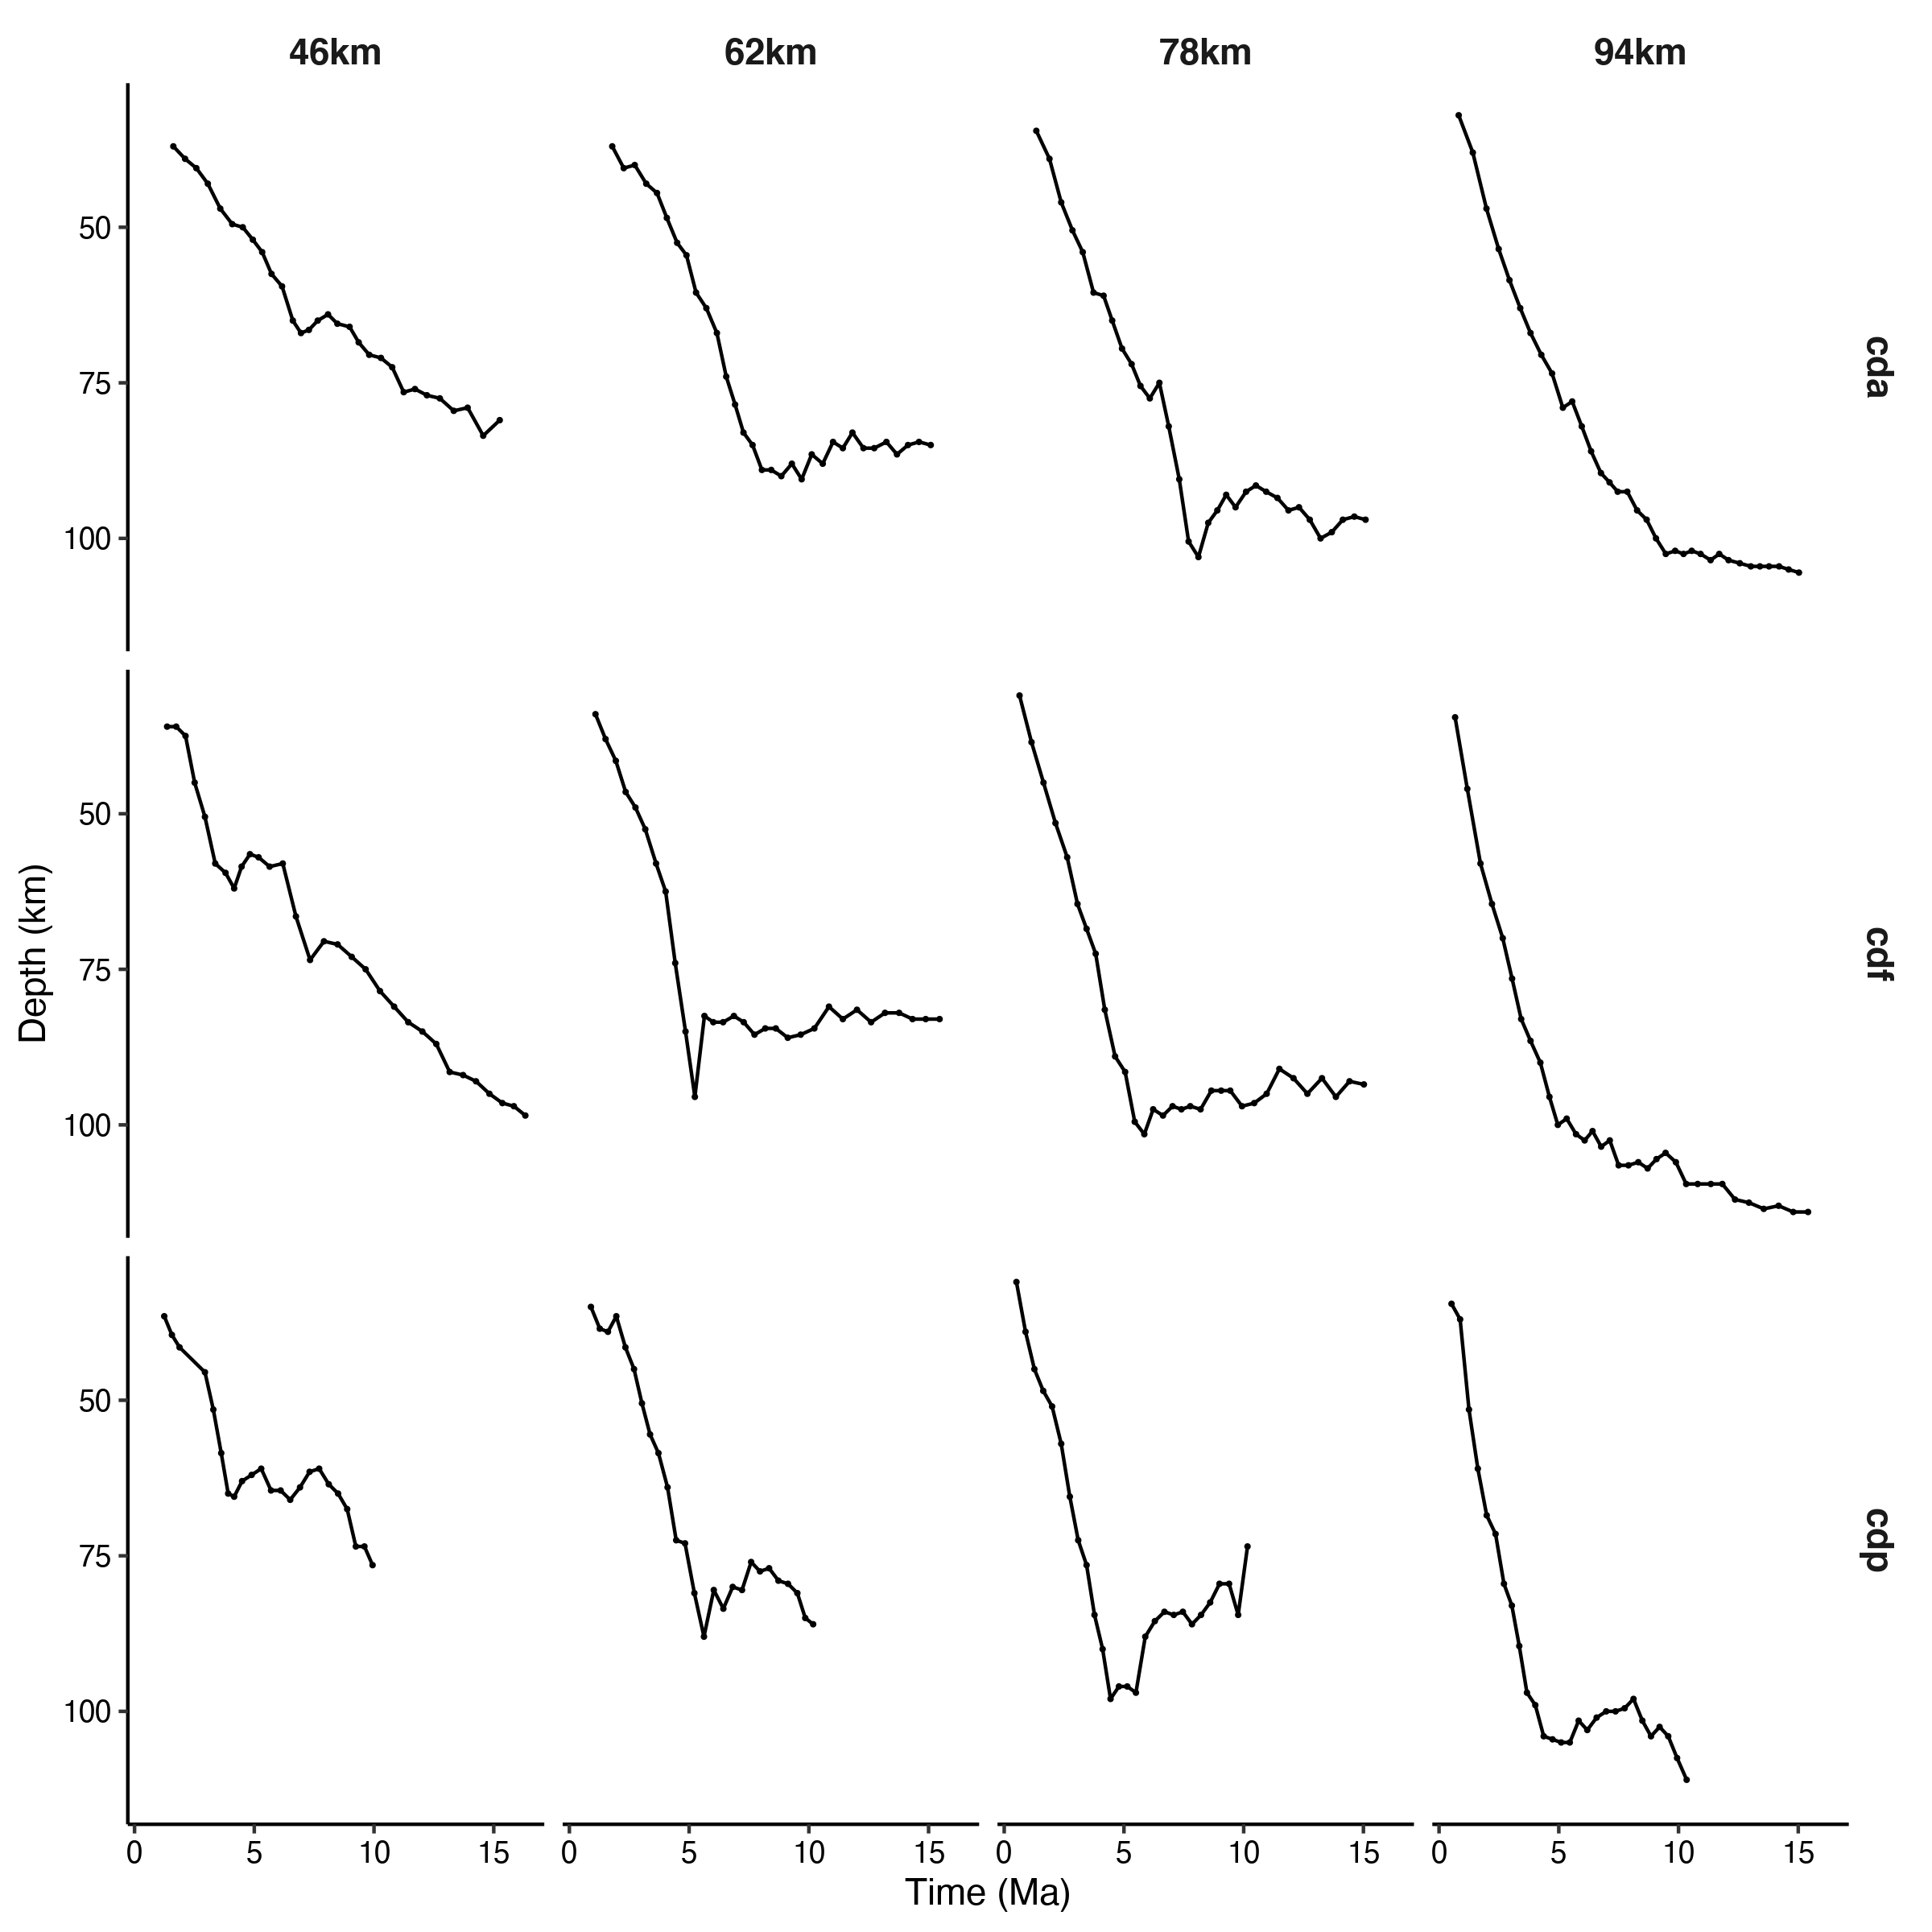
\includegraphics[width=1\linewidth,]{assets/figs/chpt2/figA1} 

}

\caption[Serpentine stability depth vs. time]{Serpentine stability depth at the plate interface vs. time for models cda, cdf, and cdp with $Z_{UP}$ = 46, 62, 78, and 94 $km$. Serpentine stabilization deepens for approximately 5 $Ma$ of subduction and then remains roughly constant for $\leq$ 10 $Ma$. The exceptions are models with very thin $Z_{UP}$, which exhibit transient behavior for at least 15 $Ma$. Overall serpentine stability depth after approximately 5 $Ma$ depends on upper-plate thickness.}\label{fig:antDepth}
\end{figure}

Numerical experiments in this chapter suggest a negative dynamic feedback regulating coupling and serpentine dehydration can help explain how similar configurations, in terms of depths to subducting plates beneath arcs (\protect\hyperlink{ref-england2004}{England et al., 2004}) and thin upper-plates (\protect\hyperlink{ref-currie2006}{Currie \& Hyndman, 2006}), may occur in subduction zones with different thermo-kinematic boundary conditions and subduction durations. The results indicate that subduction zones quickly (\(<\) 5 \(Ma\)) develop and stabilize quasi-permanent, generalized configurations with coupling depth dependent on upper-plate thickness.

Notable exceptions occur in models with the thinnest upper-plates (\(Z_{UP}\) = 46 \(km\)). Rapid extension due to thin upper-plates form spreading centers in the upper-plate within 5 \(Ma\). Passive asthenospheric upwelling near spreading centers diverts heat from deep within the upper-plate mantle. Enough heat is apparently diverted to disrupt thermal feedbacks regulating coupling and serpentine stability near the plate interface. In principle, diversion of heat from the plate interface could lead to cooler conditions, deeper serpentine stability, and thus deeper coupling. Further testing to confirm this behavior may artificially increase upper-plate strength in thin upper-plate thickness experiments to prevent high rates of spreading.

\begin{figure}[htbp]

{\centering 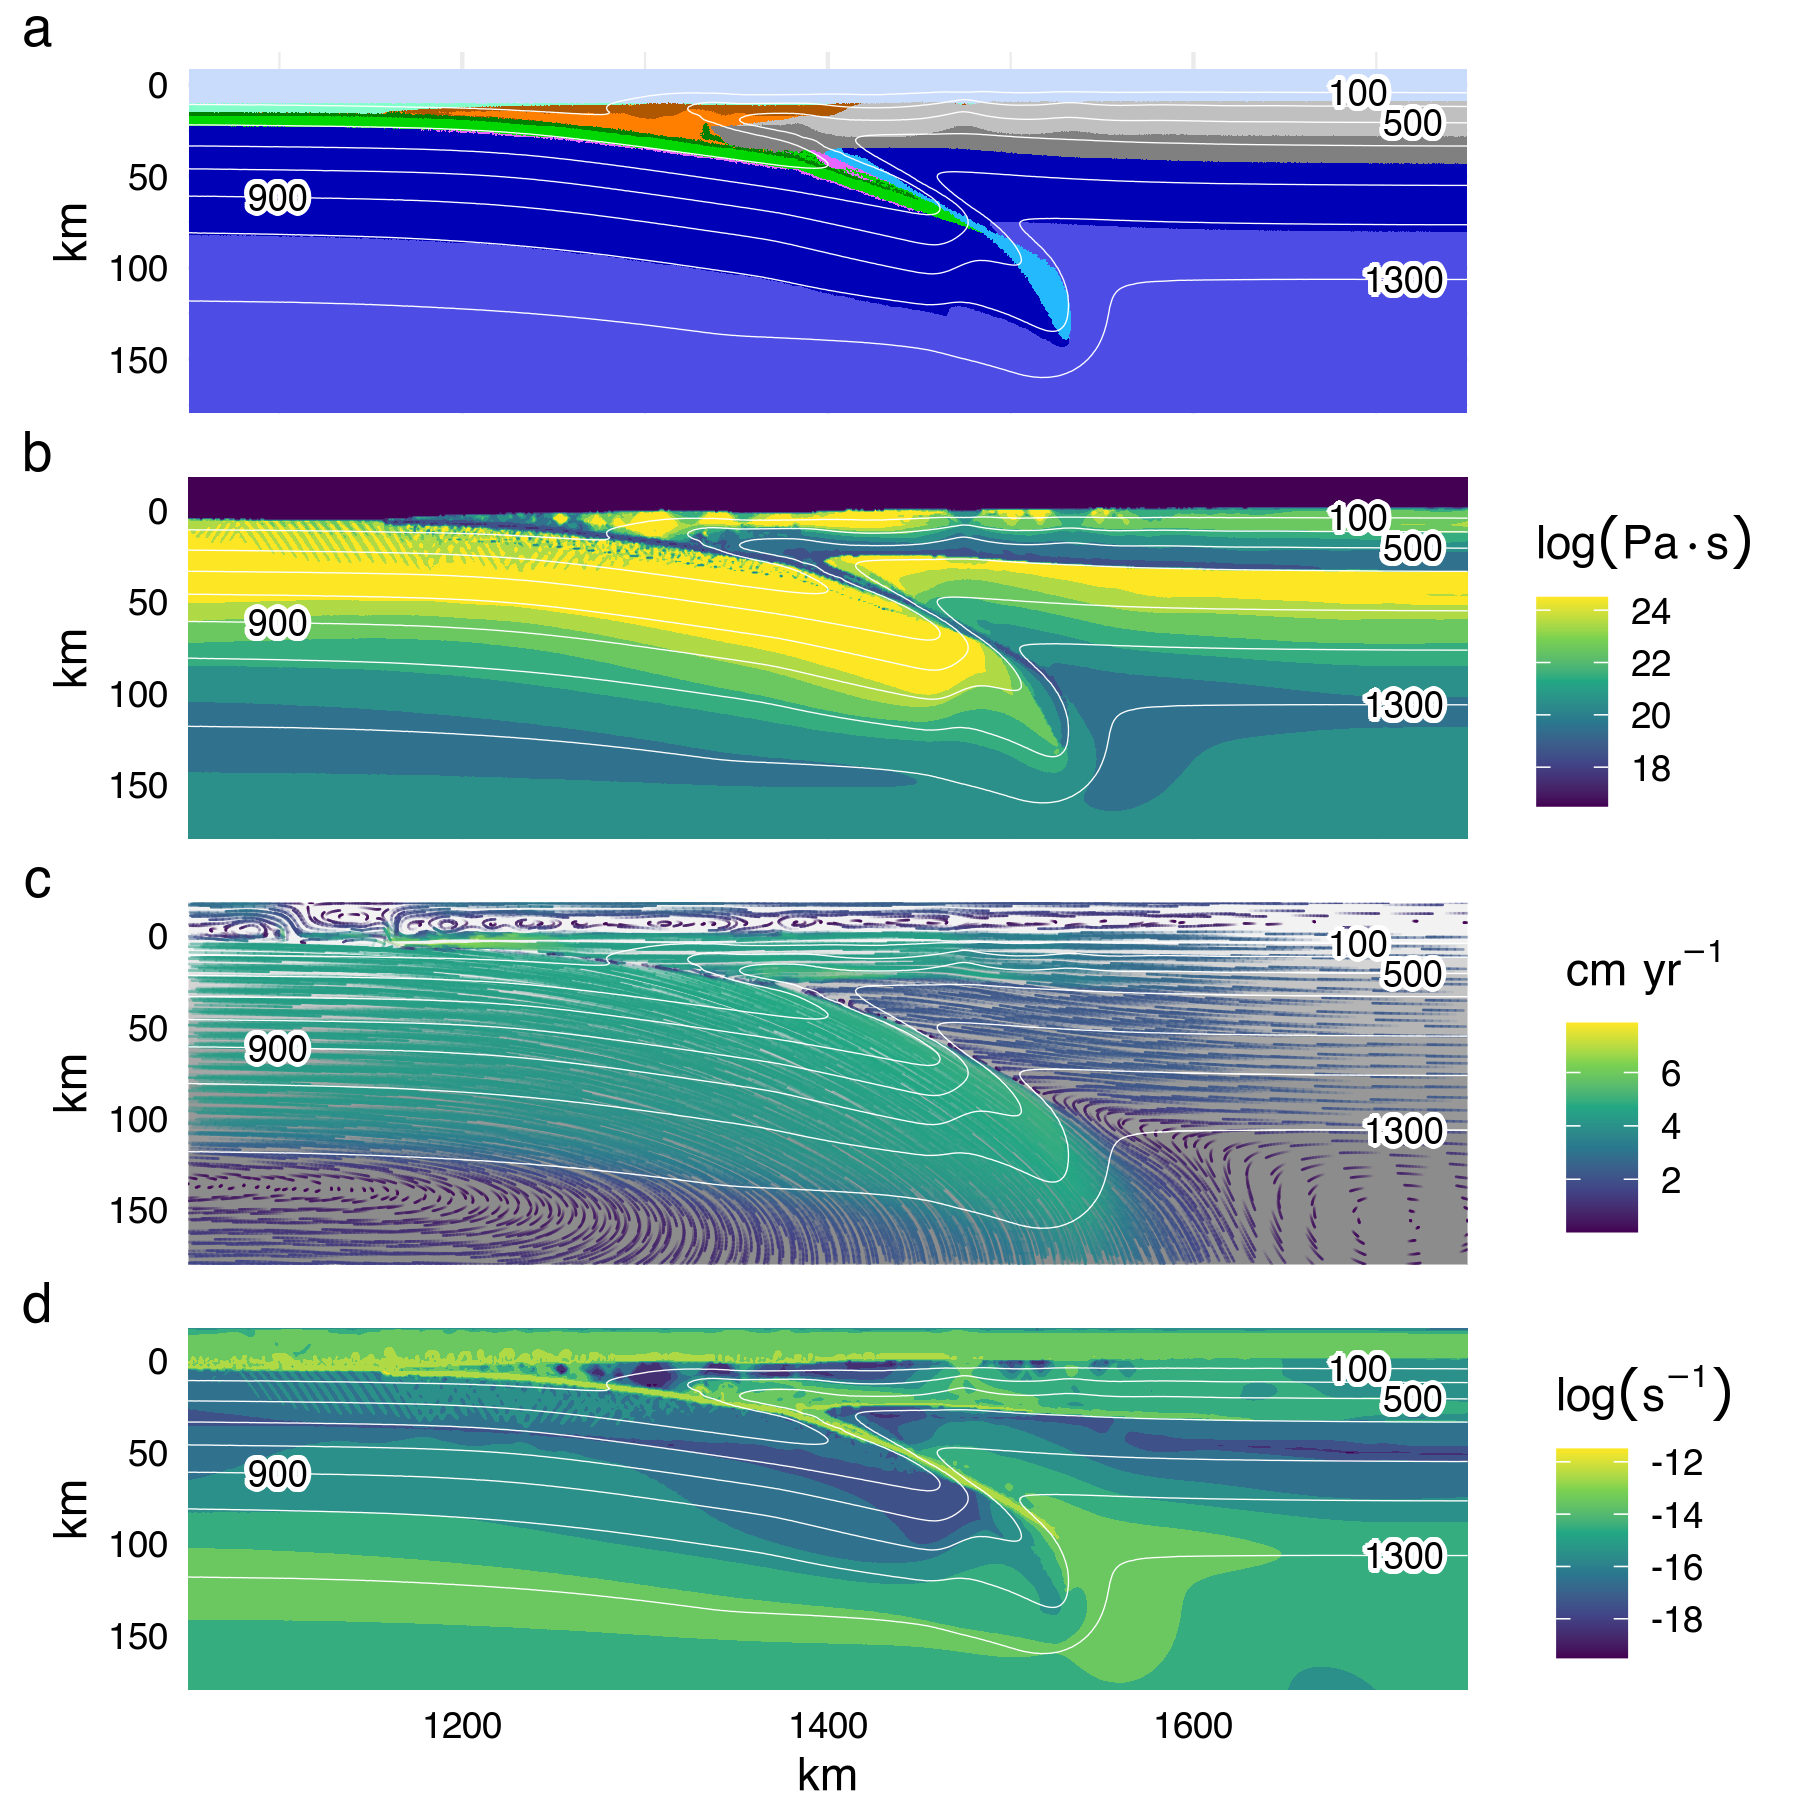
\includegraphics[width=1\linewidth,]{assets/figs/chpt2/figA2} 

}

\caption[Results for model cdf with $Z_{UP}$ = 78 $km$ at 1.64 $Ma$]{Visualizing model cdf with $Z_{UP}$ = 78 $km$ at 1.64 $Ma$. (a) Rock type. (b) Temperature. (c) Viscosity. (d) Streamlines. Early subduction is facilitated by the prescribed initial weak layer cutting the lithosphere. Strain is localized in the weak serpentine layer along the plate interface. The shallow upper-plate mantle is stagnant and loses heat to the subducting plate, promoting serpentine stabiliization to greater depths. Rock type colors are the same as Figure \ref{fig:init}.}\label{fig:cdfStep1}
\end{figure}

\begin{figure}[htbp]

{\centering 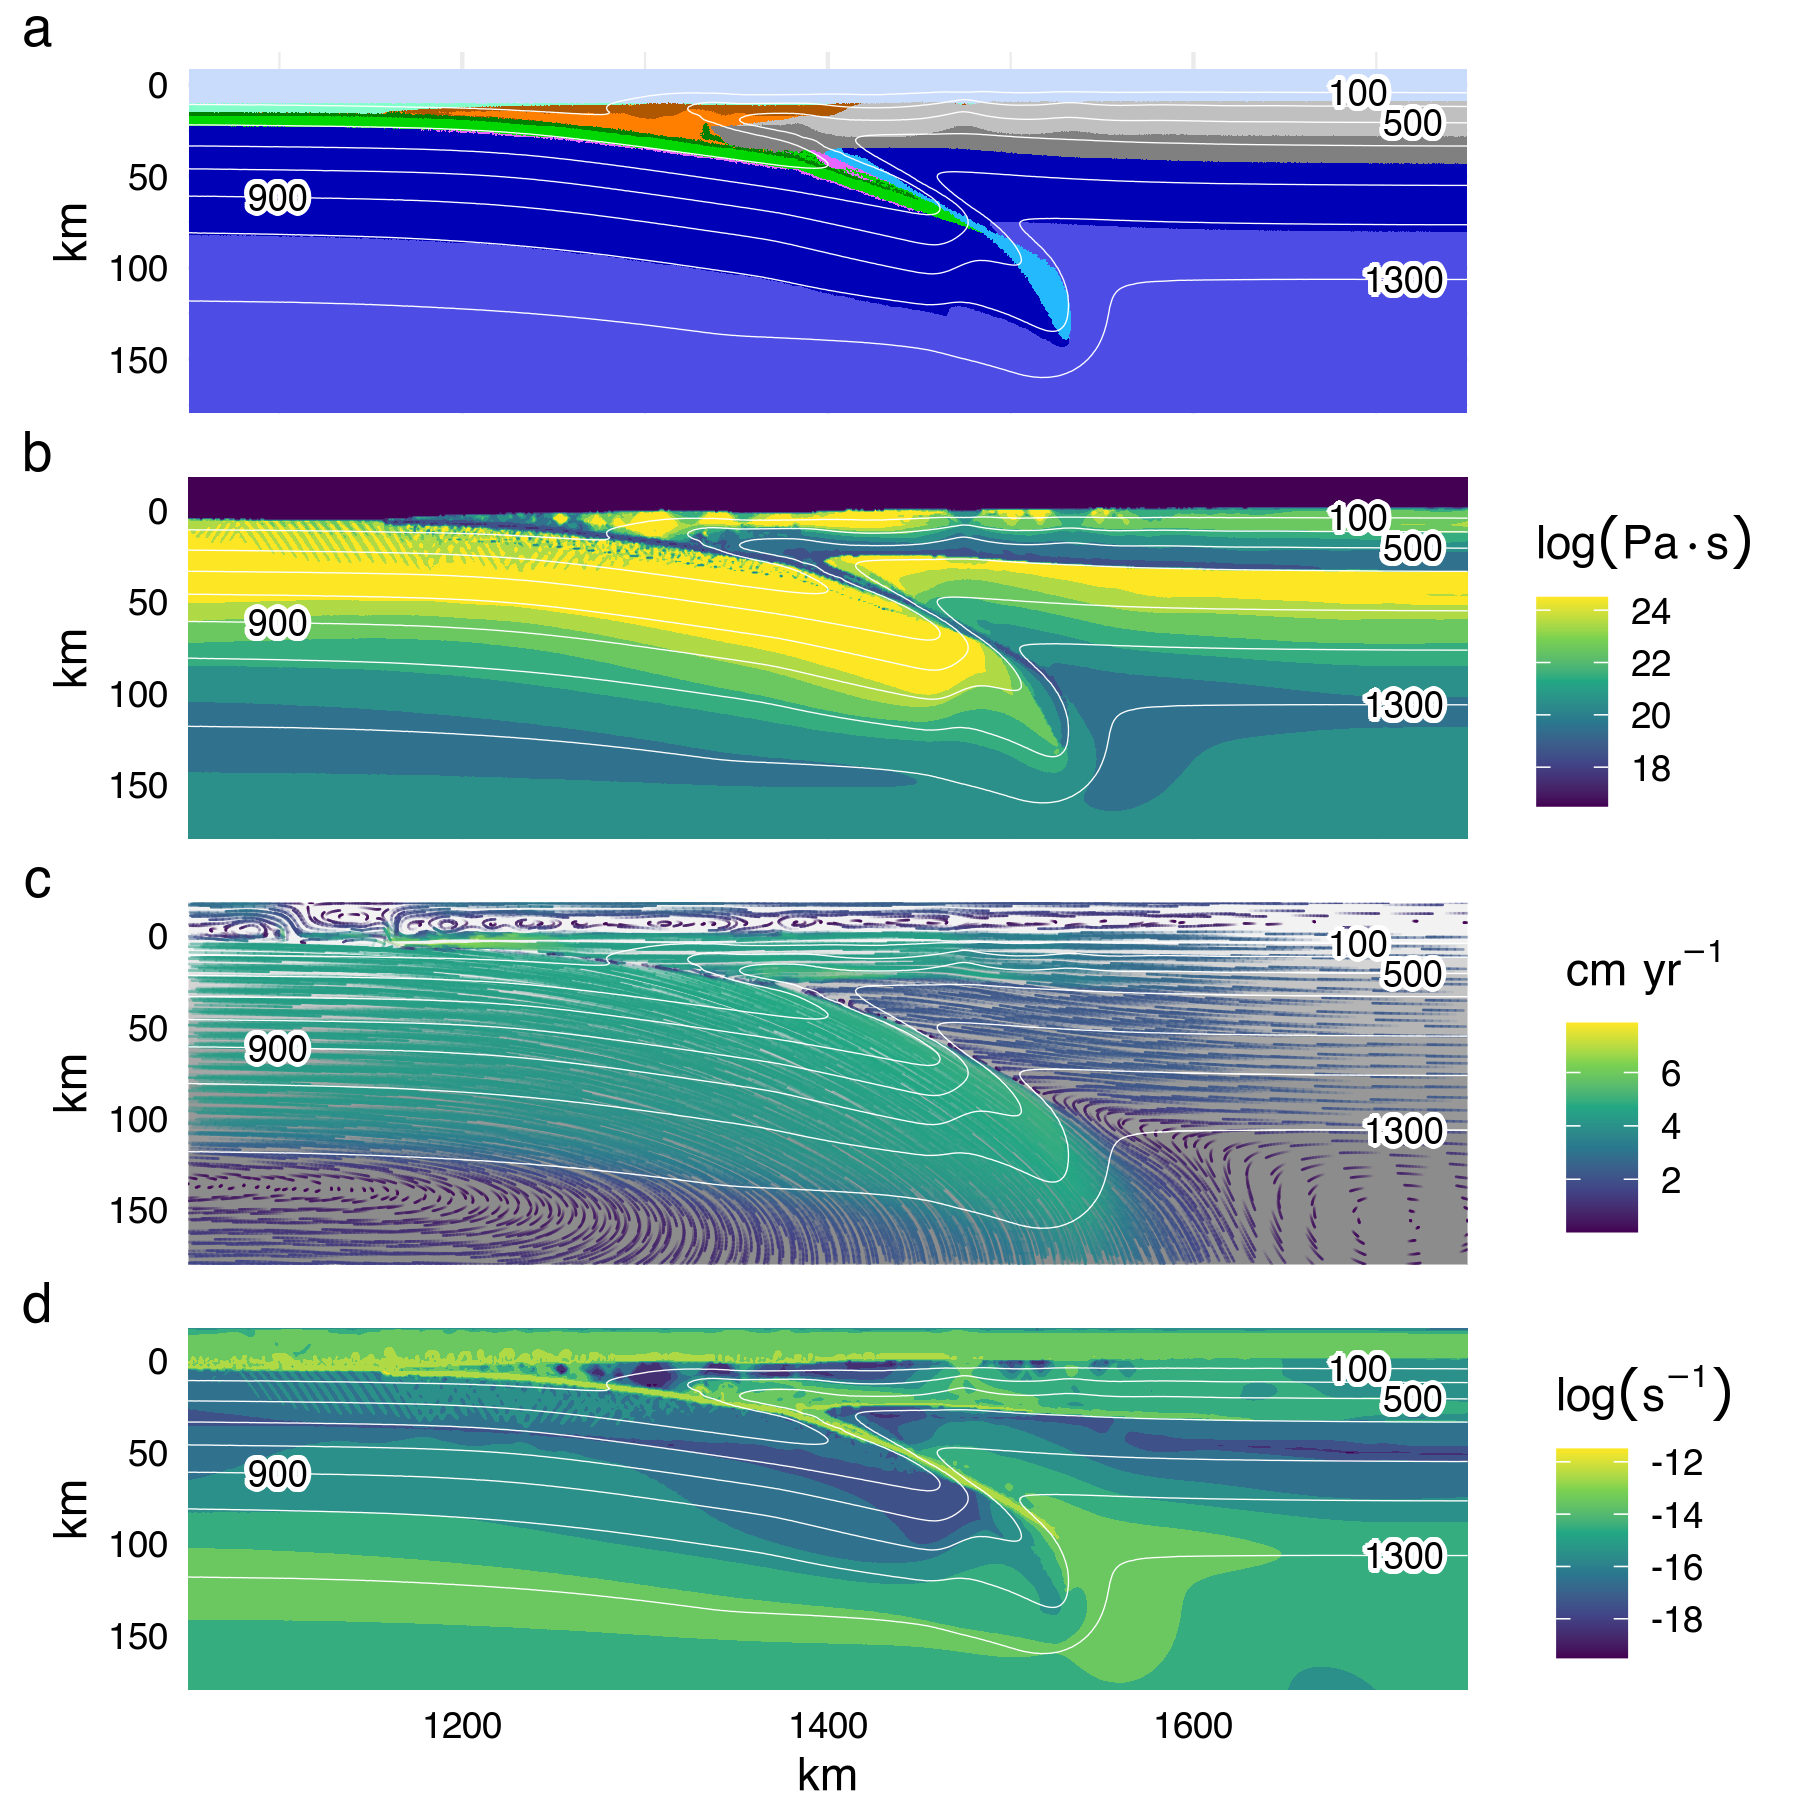
\includegraphics[width=1\linewidth,]{assets/figs/chpt2/figA3} 

}

\caption[Results for model cdf with $Z_{UP}$ = 78 $km$ at 5.05 $Ma$]{Visualizing model cdf with $Z_{UP}$ = 78 $km$ at 5.05 $Ma$. (a) Rock type. (b) Temperature. (c) Viscosity. (d) Streamlines. By 5 $Ma$ balance is achieved between cooling and heating in the shallow and deep upper-plate mantle, respectively. A feedback regulating heat transfer, serpentine destabilization, and mechanical coupling is already stabilizing coupling depth. Rock type colors are the same as Figure \ref{fig:init}.}\label{fig:cdfStep2}
\end{figure}

\begin{figure}[htbp]

{\centering 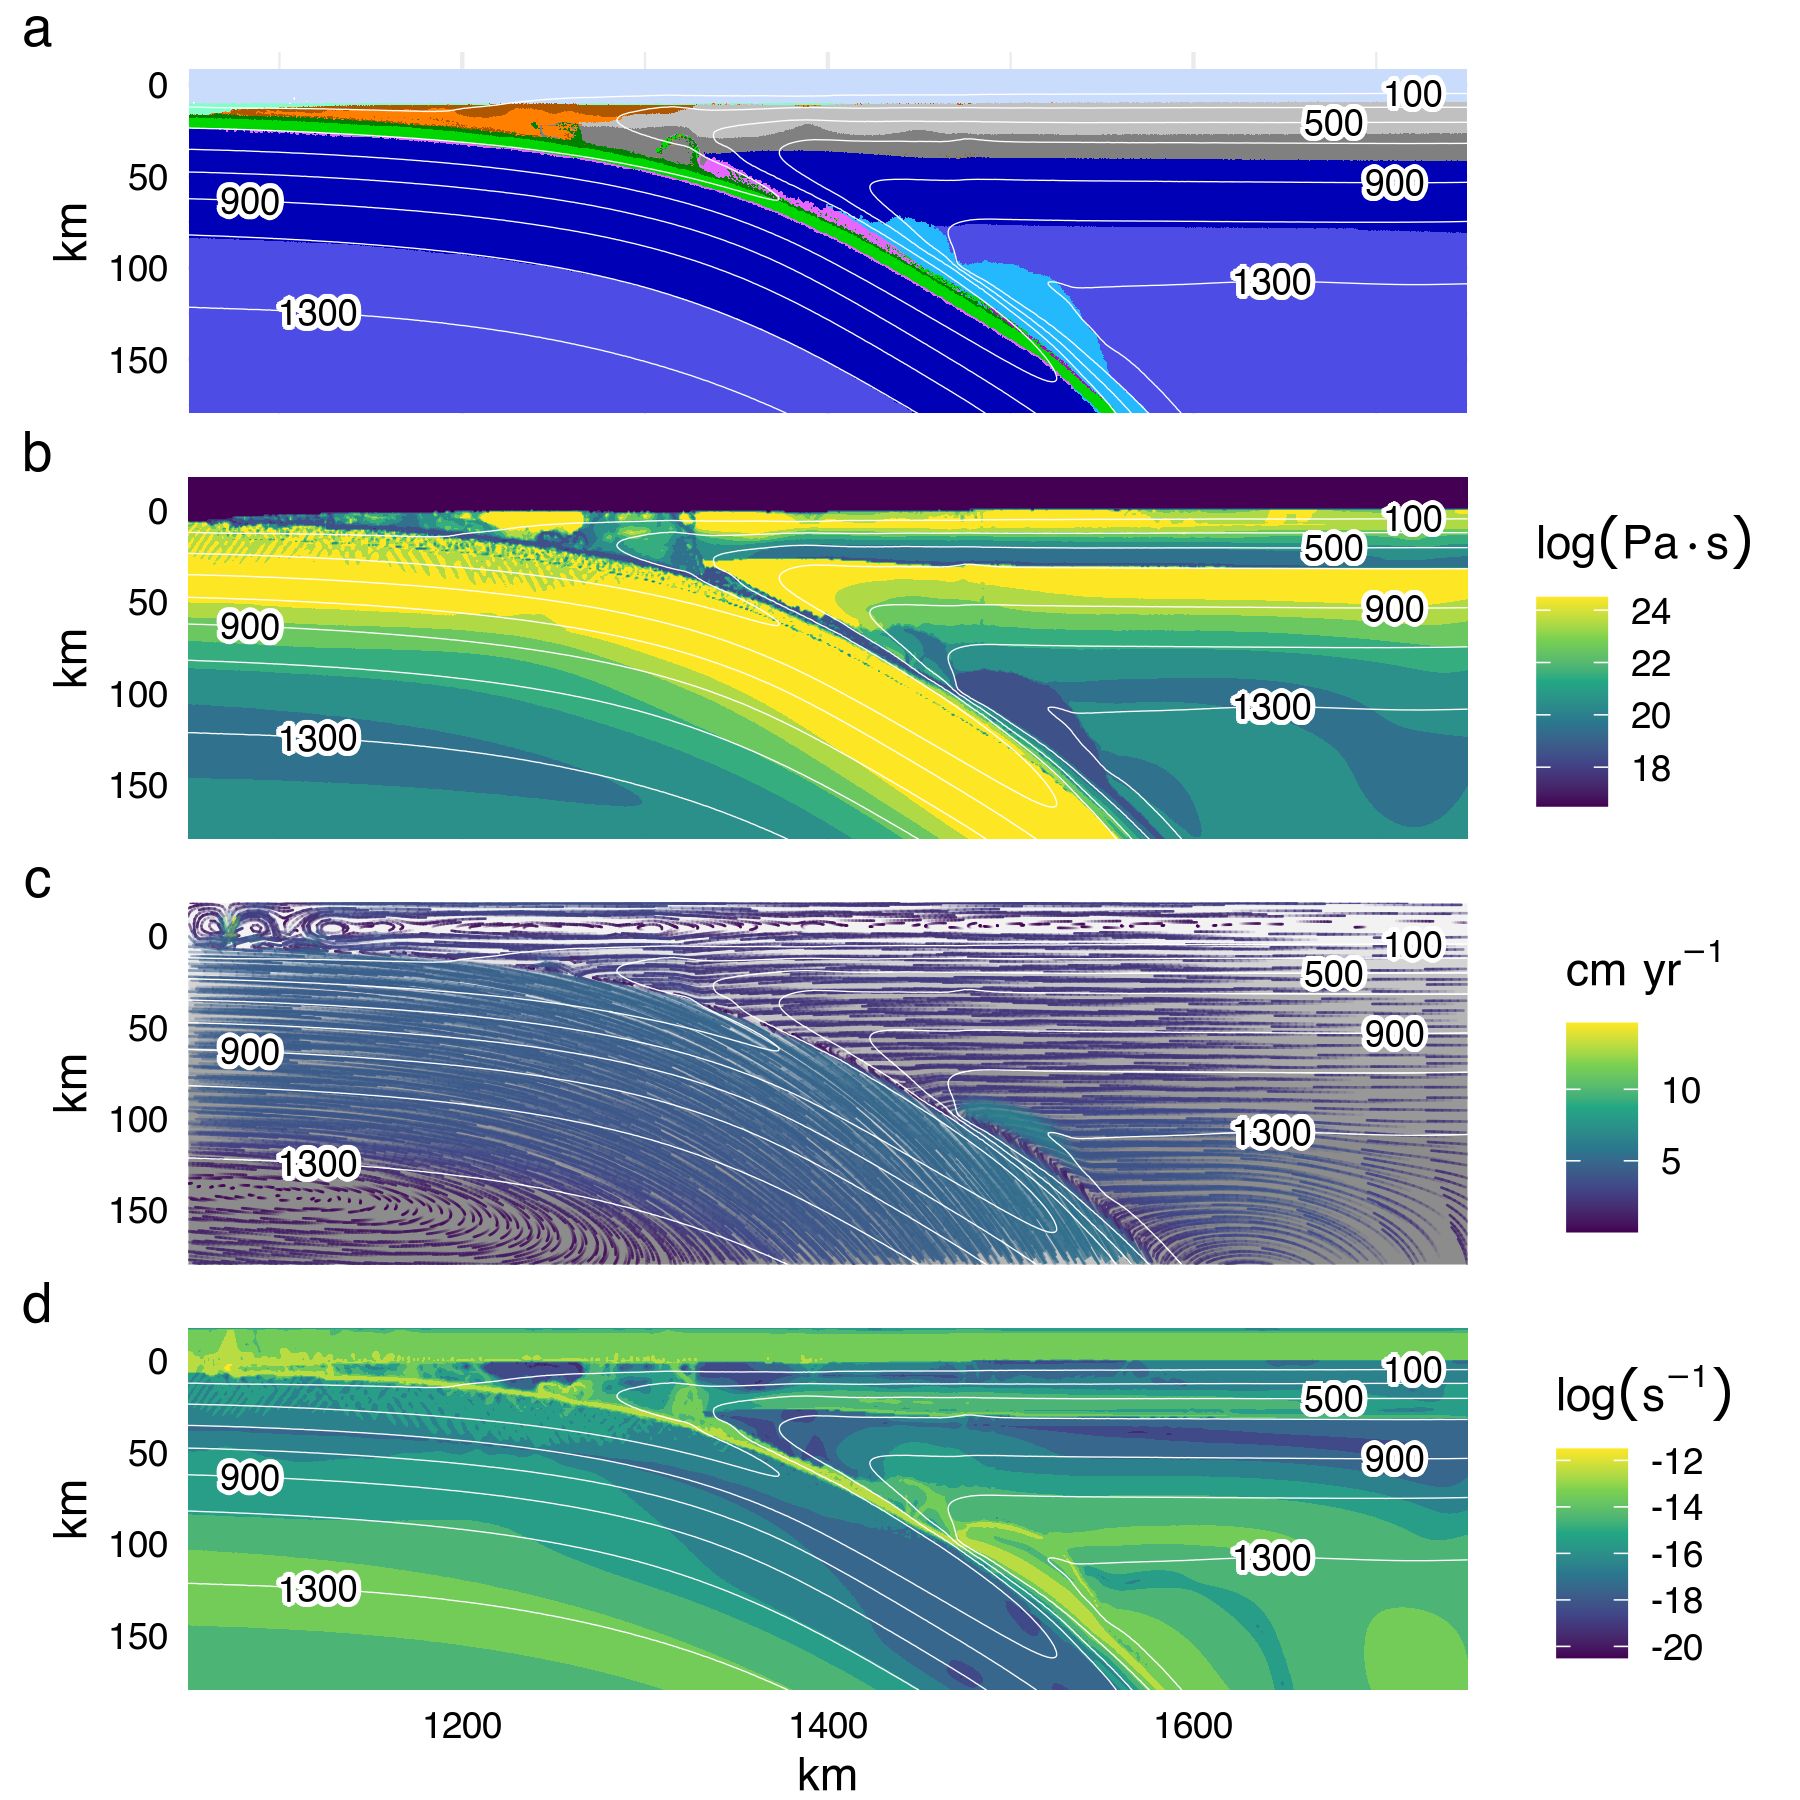
\includegraphics[width=1\linewidth,]{assets/figs/chpt2/figA4} 

}

\caption[Results for model cdf with $Z_{UP}$ = 78 $km$ at 9.93 $Ma$]{Visualizing standard model cdf with $Z_{UP}$ = 78 $km$ at 9.93 $Ma$. (a) Rock type. (b) Temperature. (c) Viscosity. (d) Streamlines. Geodynamics remain approximately constant from 5 $Ma$ (cf. Figure \ref{fig:cdfStep2}). The system remains in steady state for as long water fluxes to the upper-plate mantle and serpentine is stable. Rock type colors are the same as Figure \ref{fig:init}.}\label{fig:cdfStep3}
\end{figure}

\clearpage

\hypertarget{regSummary}{%
\section{Regression Summaries}\label{regSummary}}

The form of the preferred quadratic regression model in Section \ref{cdEstimators} (Figure \ref{fig:results} \& Table \ref{tab:zcResults}) implies a lower limit to coupling depth of approximately 60 \(km\), even for thin upper-plate thickness and, presumably, under warm conditions during nascent subduction. In principle, thin upper-plates could allow effective heat transfer in a flowing shallow asthenospheric mantle---hindering deep stabilization of serpentine. Olivine and pyroxene would be the stable mantle minerals, and strong, shallow coupling between plates would be expected Gerya et al. (\protect\hyperlink{ref-gerya2008}{2008}). However, even the warmest numerical experiments (low-\(\Phi\) \& thin upper-plate thickness) in Chapter \ref{chpt2} eventually stabilize serpentine in the shallow upper-plate mantle. This is evident by increasing depth of mechanical coupling with time for the first 5 \(Ma\) of subduction (Figure \ref{fig:antDepth}).

\begin{figure}[htbp]

{\centering 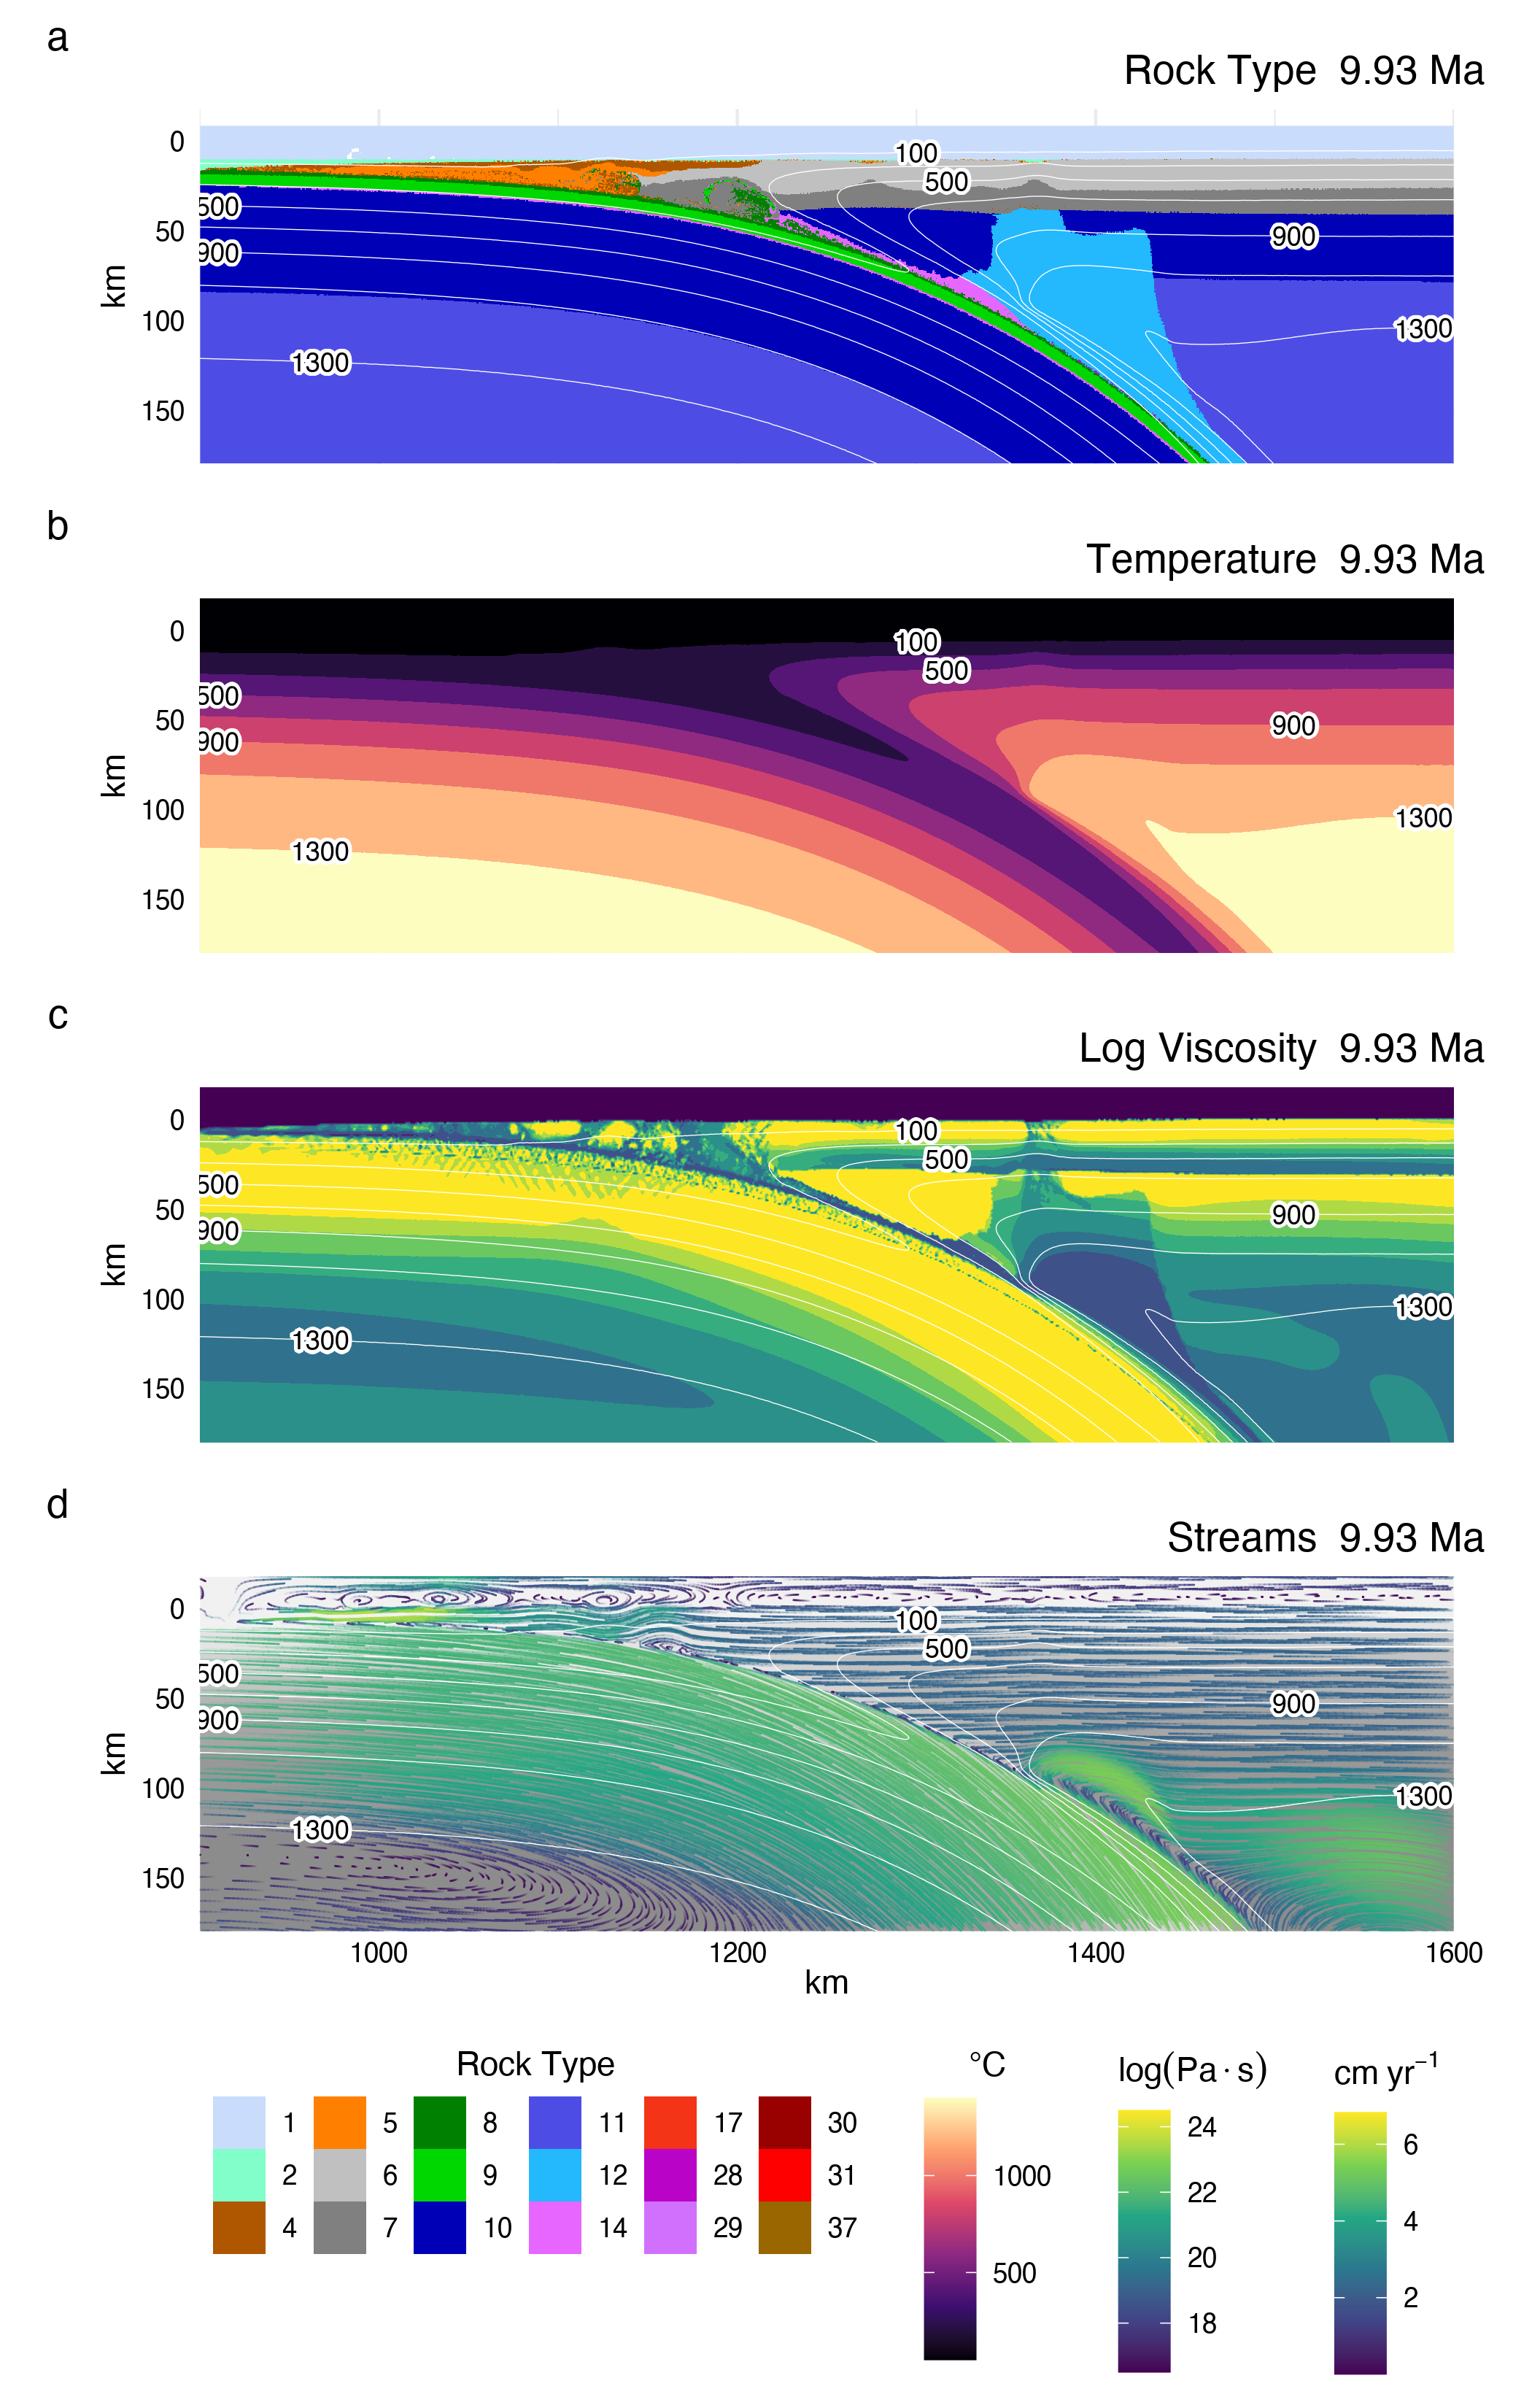
\includegraphics[width=1\linewidth,]{assets/figs/chpt2/figA5} 

}

\caption[Coupling depths determined from numerical experiments]{Coupling depths ($Z_{cpl}$, grayscale) determined from numerical experiments. Model names are listed along the top axis and correspond to the range of thermal parameter $\Phi$ values along the bottom axis. Note that the ($\Phi$) axis is not linear. $Z_{cpl}$ increases systematically with increasing $Z_{UP}$ (change in grayscale down columns) for all models. Trends in $Z_{cpl}$ with respect to $\Phi$ (change in grayscale across rows) are less apparent.}\label{fig:results}
\end{figure}

\begingroup
\renewcommand{\arraystretch}{0.5}

\begin{longtable}[t]{lrrr}
\caption{\label{tab:zcResults}Coupling depth results}\\
\toprule
Model & $Z_{UP}$ $[km]$ & $\Phi$ $[km/100]$ & $Z_{cpl}$ $[km]$\\
\midrule
\endfirsthead
\caption[]{\label{tab:zcResults}Coupling depth results \textit{(continued)}}\\
\toprule
Model & $Z_{UP}$ $[km]$ & $\Phi$ $[km/100]$ & $Z_{cpl}$ $[km]$\\
\midrule
\endhead

\endfoot
\bottomrule
\endlastfoot
\cellcolor{gray!6}{cda} & \cellcolor{gray!6}{46} & \cellcolor{gray!6}{13.0} & \cellcolor{gray!6}{66}\\
cdb & 46 & 21.5 & 74\\
\cellcolor{gray!6}{cdc} & \cellcolor{gray!6}{46} & \cellcolor{gray!6}{26.1} & \cellcolor{gray!6}{69}\\
cdd & 46 & 32.6 & 67\\
\cellcolor{gray!6}{cde} & \cellcolor{gray!6}{46} & \cellcolor{gray!6}{22.0} & \cellcolor{gray!6}{72}\\
cdf & 46 & 36.3 & 78\\
\cellcolor{gray!6}{cdg} & \cellcolor{gray!6}{46} & \cellcolor{gray!6}{44.0} & \cellcolor{gray!6}{78}\\
cdh & 46 & 55.0 & 59\\
\cellcolor{gray!6}{cdi} & \cellcolor{gray!6}{46} & \cellcolor{gray!6}{34.0} & \cellcolor{gray!6}{80}\\
cdj & 46 & 56.1 & 70\\
\cellcolor{gray!6}{cdk} & \cellcolor{gray!6}{46} & \cellcolor{gray!6}{68.0} & \cellcolor{gray!6}{58}\\
cdl & 46 & 85.0 & 65\\
\cellcolor{gray!6}{cdm} & \cellcolor{gray!6}{46} & \cellcolor{gray!6}{44.0} & \cellcolor{gray!6}{79}\\
cdn & 46 & 72.6 & 70\\
\cellcolor{gray!6}{cdo} & \cellcolor{gray!6}{46} & \cellcolor{gray!6}{88.0} & \cellcolor{gray!6}{68}\\
cdp & 46 & 110.0 & 64\\
\cellcolor{gray!6}{cda} & \cellcolor{gray!6}{62} & \cellcolor{gray!6}{13.0} & \cellcolor{gray!6}{80}\\
cdb & 62 & 21.5 & 79\\
\cellcolor{gray!6}{cdc} & \cellcolor{gray!6}{62} & \cellcolor{gray!6}{26.1} & \cellcolor{gray!6}{78}\\
cdd & 62 & 32.6 & 77\\
\cellcolor{gray!6}{cde} & \cellcolor{gray!6}{62} & \cellcolor{gray!6}{22.0} & \cellcolor{gray!6}{87}\\
cdf & 62 & 36.3 & 82\\
\cellcolor{gray!6}{cdg} & \cellcolor{gray!6}{62} & \cellcolor{gray!6}{44.0} & \cellcolor{gray!6}{75}\\
cdh & 62 & 55.0 & 70\\
\cellcolor{gray!6}{cdi} & \cellcolor{gray!6}{62} & \cellcolor{gray!6}{34.0} & \cellcolor{gray!6}{91}\\
cdj & 62 & 56.1 & 77\\
\cellcolor{gray!6}{cdk} & \cellcolor{gray!6}{62} & \cellcolor{gray!6}{68.0} & \cellcolor{gray!6}{72}\\
cdl & 62 & 85.0 & 67\\
\cellcolor{gray!6}{cdm} & \cellcolor{gray!6}{62} & \cellcolor{gray!6}{44.0} & \cellcolor{gray!6}{88}\\
cdn & 62 & 72.6 & 77\\
\cellcolor{gray!6}{cdo} & \cellcolor{gray!6}{62} & \cellcolor{gray!6}{88.0} & \cellcolor{gray!6}{74}\\
cdp & 62 & 110.0 & 75\\
\cellcolor{gray!6}{cda} & \cellcolor{gray!6}{78} & \cellcolor{gray!6}{13.0} & \cellcolor{gray!6}{87}\\
cdb & 78 & 21.5 & 94\\
\cellcolor{gray!6}{cdc} & \cellcolor{gray!6}{78} & \cellcolor{gray!6}{26.1} & \cellcolor{gray!6}{97}\\
cdd & 78 & 32.6 & 97\\
\cellcolor{gray!6}{cde} & \cellcolor{gray!6}{78} & \cellcolor{gray!6}{22.0} & \cellcolor{gray!6}{90}\\
cdf & 78 & 36.3 & 90\\
\cellcolor{gray!6}{cdg} & \cellcolor{gray!6}{78} & \cellcolor{gray!6}{44.0} & \cellcolor{gray!6}{88}\\
cdh & 78 & 55.0 & 85\\
\cellcolor{gray!6}{cdi} & \cellcolor{gray!6}{78} & \cellcolor{gray!6}{34.0} & \cellcolor{gray!6}{97}\\
cdj & 78 & 56.1 & 91\\
\cellcolor{gray!6}{cdk} & \cellcolor{gray!6}{78} & \cellcolor{gray!6}{68.0} & \cellcolor{gray!6}{84}\\
cdl & 78 & 85.0 & 77\\
\cellcolor{gray!6}{cdm} & \cellcolor{gray!6}{78} & \cellcolor{gray!6}{44.0} & \cellcolor{gray!6}{78}\\
cdn & 78 & 72.6 & 87\\
\cellcolor{gray!6}{cdo} & \cellcolor{gray!6}{78} & \cellcolor{gray!6}{88.0} & \cellcolor{gray!6}{85}\\
cdp & 78 & 110.0 & 78\\
\cellcolor{gray!6}{cda} & \cellcolor{gray!6}{94} & \cellcolor{gray!6}{13.0} & \cellcolor{gray!6}{95}\\
cdb & 94 & 21.5 & 101\\
\cellcolor{gray!6}{cdc} & \cellcolor{gray!6}{94} & \cellcolor{gray!6}{26.1} & \cellcolor{gray!6}{108}\\
cdd & 94 & 32.6 & 113\\
\cellcolor{gray!6}{cde} & \cellcolor{gray!6}{94} & \cellcolor{gray!6}{22.0} & \cellcolor{gray!6}{100}\\
cdf & 94 & 36.3 & 104\\
\cellcolor{gray!6}{cdg} & \cellcolor{gray!6}{94} & \cellcolor{gray!6}{44.0} & \cellcolor{gray!6}{104}\\
cdh & 94 & 55.0 & 104\\
\cellcolor{gray!6}{cdi} & \cellcolor{gray!6}{94} & \cellcolor{gray!6}{34.0} & \cellcolor{gray!6}{101}\\
cdj & 94 & 56.1 & 102\\
\cellcolor{gray!6}{cdk} & \cellcolor{gray!6}{94} & \cellcolor{gray!6}{68.0} & \cellcolor{gray!6}{101}\\
cdl & 94 & 85.0 & 107\\
\cellcolor{gray!6}{cdm} & \cellcolor{gray!6}{94} & \cellcolor{gray!6}{44.0} & \cellcolor{gray!6}{106}\\
cdn & 94 & 72.6 & 102\\
\cellcolor{gray!6}{cdo} & \cellcolor{gray!6}{94} & \cellcolor{gray!6}{88.0} & \cellcolor{gray!6}{98}\\
cdp & 94 & 110.0 & 108\\*
\end{longtable}

\endgroup

Summary statistics for the regression models presented in Section \ref{cdEstimators} are given in Tables \ref{tab:anova} and \ref{tab:regSummary}.

\begin{table}

\caption{\label{tab:anova}Summary of ANOVA test}
\centering
\begin{threeparttable}
\begin{tabular}[t]{lrrrl}
\toprule
\multicolumn{1}{c}{$Z_{UP}$ Groups} & \multicolumn{1}{c}{$Z_{cpl}$ Estimate} & \multicolumn{1}{c}{Upper Bound} & \multicolumn{1}{c}{Lower Bound} & \multicolumn{1}{c}{p value} \\
\multicolumn{1}{c}{} & \multicolumn{1}{c}{$[km]$} & \multicolumn{1}{c}{$[km]$} & \multicolumn{1}{c}{$[km]$} & \multicolumn{1}{c}{}\\
\midrule
\cellcolor{gray!6}{62-46} & \cellcolor{gray!6}{8.3} & \cellcolor{gray!6}{2.5} & \cellcolor{gray!6}{14.0} & \cellcolor{gray!6}{1.84e-03}\\
78-46 & 18.0 & 12.3 & 23.7 & 1.08e-10\\
\cellcolor{gray!6}{94-46} & \cellcolor{gray!6}{33.6} & \cellcolor{gray!6}{27.8} & \cellcolor{gray!6}{39.3} & \cellcolor{gray!6}{1.99e-11}\\
78-62 & 9.8 & 4.0 & 15.5 & 1.83e-04\\
\cellcolor{gray!6}{94-62} & \cellcolor{gray!6}{25.3} & \cellcolor{gray!6}{19.6} & \cellcolor{gray!6}{31.0} & \cellcolor{gray!6}{1.99e-11}\\
\addlinespace
94-78 & 15.6 & 9.8 & 21.3 & 7.31e-09\\
\bottomrule
\end{tabular}
\begin{tablenotes}
\item Pair-wise Tukey's test comparing means between groups. Estimates are differences between means. Null hypothesis is that means are not different
\end{tablenotes}
\end{threeparttable}
\end{table}

\begin{table}

\caption{\label{tab:regSummary}Summary of regression models}
\centering
\begin{threeparttable}
\begin{tabular}[t]{llrrl}
\toprule
Model & Term & Estimate & Std. Error & p value\\
\midrule
\cellcolor{gray!6}{1} & \cellcolor{gray!6}{Intercept} & \cellcolor{gray!6}{89.4} & \cellcolor{gray!6}{3.7} & \cellcolor{gray!6}{2.24e-33}\\
1 & $\phi$ & -0.1 & 0.1 & 1.55e-01\\
\cellcolor{gray!6}{2} & \cellcolor{gray!6}{Intercept} & \cellcolor{gray!6}{36.4} & \cellcolor{gray!6}{3.2} & \cellcolor{gray!6}{7.15e-17}\\
2 & $Z_{UP}$ & 0.7 & 0.0 & 3.73e-23\\
\cellcolor{gray!6}{3} & \cellcolor{gray!6}{Intercept} & \cellcolor{gray!6}{58.9} & \cellcolor{gray!6}{1.7} & \cellcolor{gray!6}{1.43e-41}\\
\addlinespace
3 & $Z_{UP}^2$ & 0.0 & 0.0 & 2.98e-24\\
\cellcolor{gray!6}{4} & \cellcolor{gray!6}{Intercept} & \cellcolor{gray!6}{69.2} & \cellcolor{gray!6}{14.0} & \cellcolor{gray!6}{6.25e-06}\\
4 & $Z_{UP}$ & -0.3 & 0.4 & 4.63e-01\\
\cellcolor{gray!6}{4} & \cellcolor{gray!6}{$Z_{UP}^2$} & \cellcolor{gray!6}{0.0} & \cellcolor{gray!6}{0.0} & \cellcolor{gray!6}{1.95e-02}\\
5 & Intercept & 41.1 & 3.3 & 1.14e-18\\
\addlinespace
\cellcolor{gray!6}{5} & \cellcolor{gray!6}{$Z_{UP}$} & \cellcolor{gray!6}{0.7} & \cellcolor{gray!6}{0.0} & \cellcolor{gray!6}{1.12e-24}\\
5 & $\phi$ & -0.1 & 0.0 & 1.18e-03\\
\cellcolor{gray!6}{6} & \cellcolor{gray!6}{Intercept} & \cellcolor{gray!6}{63.6} & \cellcolor{gray!6}{2.1} & \cellcolor{gray!6}{8.29e-39}\\
6 & $Z_{UP}^2$ & 0.0 & 0.0 & 5.68e-26\\
\cellcolor{gray!6}{6} & \cellcolor{gray!6}{$\phi$} & \cellcolor{gray!6}{-0.1} & \cellcolor{gray!6}{0.0} & \cellcolor{gray!6}{6.98e-04}\\
\addlinespace
7 & Intercept & 73.8 & 12.9 & 3.39e-07\\
\cellcolor{gray!6}{7} & \cellcolor{gray!6}{$Z_{UP}$} & \cellcolor{gray!6}{-0.3} & \cellcolor{gray!6}{0.4} & \cellcolor{gray!6}{4.23e-01}\\
7 & $Z_{UP}^2$ & 0.0 & 0.0 & 1.12e-02\\
\cellcolor{gray!6}{7} & \cellcolor{gray!6}{$\phi$} & \cellcolor{gray!6}{-0.1} & \cellcolor{gray!6}{0.0} & \cellcolor{gray!6}{7.28e-04}\\
\bottomrule
\end{tabular}
\begin{tablenotes}
\item \uline{\textit{models}}: 1: $[z_c=\phi]$, 2: $[z_c=Z_{UP}]$, 3: $[z_c=Z_{UP}^2]$, 4: $[z_c=Z_{UP}+Z_{UP}^2]$, 5: $[z_c=Z_{UP}+\phi]$, 6: [$z_c=Z_{UP}^2+\phi]$, 7: $[z_c=Z_{UP}+Z_{UP}^2+\phi]$
\end{tablenotes}
\end{threeparttable}
\end{table}

\begin{figure}[htbp]

{\centering 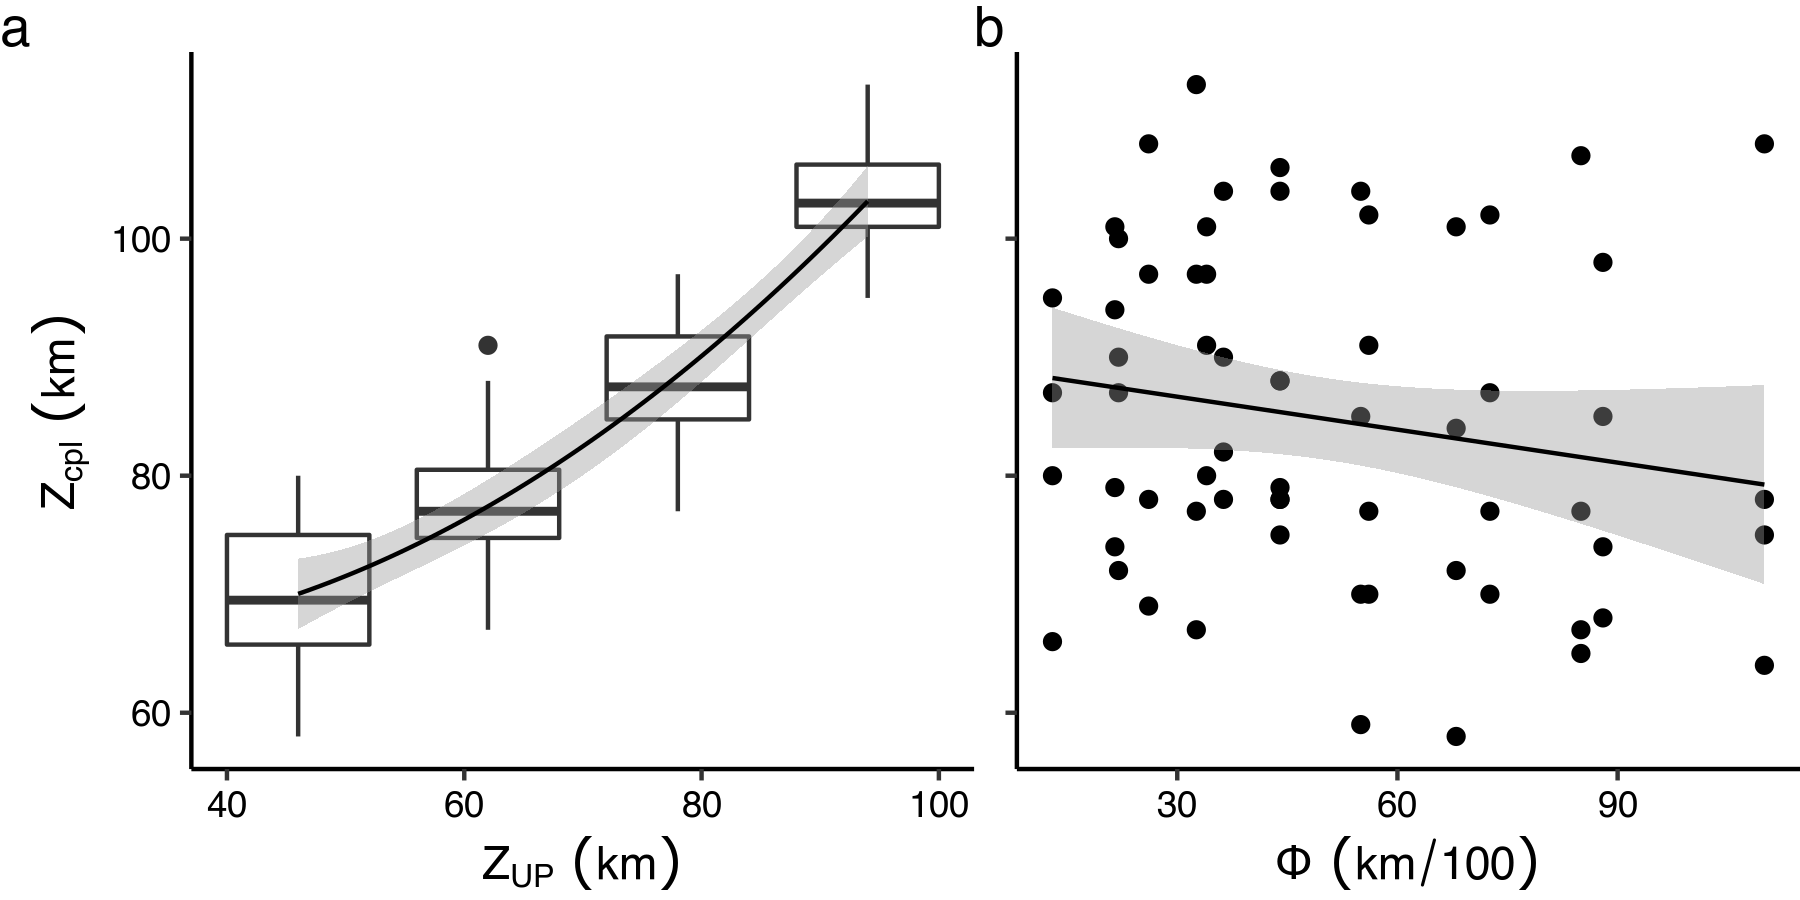
\includegraphics[width=1\linewidth,]{assets/figs/chpt2/figA6} 

}

\caption[Bivariate regressions of coupling results]{Bivariate regressions. (a) Coupling depth ($Z_{cpl}$) vs. upper-plate thickness ($Z_{UP}$) shows $Z_{cpl}$ increasing approximately quadratically with increasing $Z_{UP}$. The correlation is highly significant (see Tables \ref{tab:anova} and \ref{tab:regSummary}) and explains more than 80\% of the variance in $Z_{cpl}$. $Z_{UP}$ alone estimates $Z_{cpl}$ well. (b) $Z_{cpl}$ vs. thermal parameter ($\Phi$) shows no significant correlation (no line fits with a slope significantly different from zero). $\Phi$ has little effect on $Z_{cpl}$ and cannot be used as a standalone estimator.}\label{fig:biv}
\end{figure}

\clearpage

\hypertarget{deHydration}{%
\section{(De)hydration Model}\label{deHydration}}

The material properties used in the numerical experiments are listed in Table \ref{tab:materials} and Table \ref{tab:melts}. For details about the sedimentation and erosion, melting and extraction, and rheological models, please refer to Sizova et al. (\protect\hyperlink{ref-sizova2010}{2010}). Here we discuss only the hydrodynamic model, because it is the most relevant aspect of the numerical experiments.

Hydrodynamics in the numerical models control the timing and magnitude of mantle wedge hydration. The main sources of water delivered to the mantle are altered basaltic crust and seafloor sediments, which we assumed to contain up to 5 \(wt.\% H_{2}O\). We assumed a gradual expulsion of water from pore space and through quasi-continuous dehydration reactions occurring within the slab. Water content is computed using the following equation:
\DIFdelbegin %DIFDELCMD < 

%DIFDELCMD < %%%
\DIFdelend \begin{equation}
  \chi_{H_{2}O} = \chi_{H_{2}O_{init}}\times\left(1-\frac{\Delta z}{150\times 10^{3}}\right)
\end{equation}
\DIFdelbegin %DIFDELCMD < 

%DIFDELCMD < %%%
\DIFdelend where \(\chi_{H_{2}O_{init}}\) = 5 \(wt.\%\) and \(\Delta z\) is a marker's depth below the topographical surface.

If a rock marker dehydrates, an independent water particle is instantaneously generated at the same location with the respective \(H_{2}O\) content. The new water particle is moved in accordance to the local velocity field, described by the following equation:
\DIFdelbegin %DIFDELCMD < 

%DIFDELCMD < %%%
\DIFdelend \begin{equation}
  \begin{aligned}
    \vec{v}_{\text{water}} & = (\vec{v}_x,\ \vec{v}_z) \\
    \vec{v}_z & = \vec{v}_z - \vec{v}_{z(\text{percolation})} \\
  \end{aligned}
\end{equation}
\DIFdelbegin %DIFDELCMD < 

%DIFDELCMD < %%%
\DIFdelend where \(\vec{v}_{water}\) is the velocity vector of the water particle, \(\vec{v}_{x}\) and \(\vec{v}_{z}\) are the local velocity vectors of the solid state mantle or crust, and \(\vec{v}_{z(percolation)}\) is a imposed constant upward percolation velocity (10 \(cm/year\)). We implicitly neglect kinetics of reactions, as material properties of markers change instantaneously at equilibrium reactions.

\DIFaddbegin \begin{landscape}\DIFaddend \begin{table}

\caption{\label{tab:melts}Melting curves used in numerical experiments}
\centering
\DIFdelbeginFL %DIFDELCMD < \resizebox{\linewidth}{!}{
%DIFDELCMD < \begin{threeparttable}
%DIFDELCMD < \begin{tabular}[t]{lrrlrlrllrr}
%DIFDELCMD < \toprule
%DIFDELCMD < Material & a & b & c & d & e & f & g & h & i & j\\
%DIFDELCMD < \midrule
%DIFDELCMD < \cellcolor{gray!6}{sediments} & \cellcolor{gray!6}{1200} & \cellcolor{gray!6}{889} & \cellcolor{gray!6}{1.79e+04} & \cellcolor{gray!6}{54} & \cellcolor{gray!6}{2.02e+04} & \cellcolor{gray!6}{831} & \cellcolor{gray!6}{6.00e-02} & \cellcolor{gray!6}{} & \cellcolor{gray!6}{1262} & \cellcolor{gray!6}{0.009}\\
%DIFDELCMD < felsic crust & 1200 & 889 & 1.79e+04 & 54 & 2.02e+04 & 831 & 6.00e-02 &  & 1262 & 0.009\\
%DIFDELCMD < \cellcolor{gray!6}{basalt} & \cellcolor{gray!6}{1600} & \cellcolor{gray!6}{973} & \cellcolor{gray!6}{7.04e+05} & \cellcolor{gray!6}{354} & \cellcolor{gray!6}{7.78e+07} & \cellcolor{gray!6}{935} & \cellcolor{gray!6}{3.50e-03} & \cellcolor{gray!6}{6.2e-05} & \cellcolor{gray!6}{1423} & \cellcolor{gray!6}{0.105}\\
%DIFDELCMD < gabbro & 1600 & 973 & 7.04e+05 & 354 & 7.78e+07 & 935 & 3.50e-03 & 6.2e-05 & 1423 & 0.105\\
%DIFDELCMD < \cellcolor{gray!6}{mantle dry} & \cellcolor{gray!6}{} & \cellcolor{gray!6}{} & \cellcolor{gray!6}{} & \cellcolor{gray!6}{} & \cellcolor{gray!6}{} & \cellcolor{gray!6}{1394} & \cellcolor{gray!6}{1.33e-01} & \cellcolor{gray!6}{-5.1e-05} & \cellcolor{gray!6}{2073} & \cellcolor{gray!6}{0.114}\\
%DIFDELCMD < mantle hydrated & 2400 & 1240 & 4.98e+04 & 323 &  &  & 1.27e+05 & 3.5e-05 & 2073 & 0.114\\
%DIFDELCMD < \cellcolor{gray!6}{serpentine} & \cellcolor{gray!6}{2400} & \cellcolor{gray!6}{1240} & \cellcolor{gray!6}{4.98e+04} & \cellcolor{gray!6}{323} & \cellcolor{gray!6}{} & \cellcolor{gray!6}{} & \cellcolor{gray!6}{1.27e+05} & \cellcolor{gray!6}{3.5e-05} & \cellcolor{gray!6}{2073} & \cellcolor{gray!6}{0.114}\\
%DIFDELCMD < \bottomrule
%DIFDELCMD < \end{tabular}
%DIFDELCMD < \begin{tablenotes}
%DIFDELCMD < \item \uline{\textit{solidus curve}}: $T(P)=[b+\frac{c}{(P+d)}+\frac{e}{(P+d)^2}]$ at $P<a$ and $[f+gP+hP^2]$ at $P\geq a$
%DIFDELCMD < \item \uline{\textit{liquidus curve}}: $T(P) = i+jP$ with $T$ in $[K]$ and $P$ in $[MPa]$
%DIFDELCMD < \item \uline{\textit{reference}}: Schmidt \& Poli (1998)
%DIFDELCMD < \end{tablenotes}
%DIFDELCMD < \end{threeparttable}}
%DIFDELCMD < %%%
\DIFdelendFL \DIFaddbeginFL \begin{threeparttable}
\begin{tabular}[t]{lrrlrlrllrr}
\toprule
\DIFaddFL{Material }& \DIFaddFL{a }& \DIFaddFL{b }& \DIFaddFL{c }& \DIFaddFL{d }& \DIFaddFL{e }& \DIFaddFL{f }& \DIFaddFL{g }& \DIFaddFL{h }& \DIFaddFL{i }& \DIFaddFL{j}\\
\midrule
\cellcolor{gray!6}{sediments} & \cellcolor{gray!6}{1200} & \cellcolor{gray!6}{889} & \cellcolor{gray!6}{1.79e+04} & \cellcolor{gray!6}{54} & \cellcolor{gray!6}{2.02e+04} & \cellcolor{gray!6}{831} & \cellcolor{gray!6}{6.00e-02} & \cellcolor{gray!6}{} & \cellcolor{gray!6}{1262} & \cellcolor{gray!6}{0.009}\\
\DIFaddFL{felsic crust }& \DIFaddFL{1200 }& \DIFaddFL{889 }& \DIFaddFL{1.79e+04 }& \DIFaddFL{54 }& \DIFaddFL{2.02e+04 }& \DIFaddFL{831 }& \DIFaddFL{6.00e-02 }&  & \DIFaddFL{1262 }& \DIFaddFL{0.009}\\
\cellcolor{gray!6}{basalt} & \cellcolor{gray!6}{1600} & \cellcolor{gray!6}{973} & \cellcolor{gray!6}{7.04e+05} & \cellcolor{gray!6}{354} & \cellcolor{gray!6}{7.78e+07} & \cellcolor{gray!6}{935} & \cellcolor{gray!6}{3.50e-03} & \cellcolor{gray!6}{6.2e-05} & \cellcolor{gray!6}{1423} & \cellcolor{gray!6}{0.105}\\
\DIFaddFL{gabbro }& \DIFaddFL{1600 }& \DIFaddFL{973 }& \DIFaddFL{7.04e+05 }& \DIFaddFL{354 }& \DIFaddFL{7.78e+07 }& \DIFaddFL{935 }& \DIFaddFL{3.50e-03 }& \DIFaddFL{6.2e-05 }& \DIFaddFL{1423 }& \DIFaddFL{0.105}\\
\cellcolor{gray!6}{mantle dry} & \cellcolor{gray!6}{} & \cellcolor{gray!6}{} & \cellcolor{gray!6}{} & \cellcolor{gray!6}{} & \cellcolor{gray!6}{} & \cellcolor{gray!6}{1394} & \cellcolor{gray!6}{1.33e-01} & \cellcolor{gray!6}{-5.1e-05} & \cellcolor{gray!6}{2073} & \cellcolor{gray!6}{0.114}\\
\DIFaddFL{mantle hydrated }& \DIFaddFL{2400 }& \DIFaddFL{1240 }& \DIFaddFL{4.98e+04 }& \DIFaddFL{323 }&  &  & \DIFaddFL{1.27e+05 }& \DIFaddFL{3.5e-05 }& \DIFaddFL{2073 }& \DIFaddFL{0.114}\\
\cellcolor{gray!6}{serpentine} & \cellcolor{gray!6}{2400} & \cellcolor{gray!6}{1240} & \cellcolor{gray!6}{4.98e+04} & \cellcolor{gray!6}{323} & \cellcolor{gray!6}{} & \cellcolor{gray!6}{} & \cellcolor{gray!6}{1.27e+05} & \cellcolor{gray!6}{3.5e-05} & \cellcolor{gray!6}{2073} & \cellcolor{gray!6}{0.114}\\
\bottomrule
\end{tabular}
\begin{tablenotes}
\item \uline{\textit{solidus curve}}\DIFaddFL{: $T(P)=[b+\frac{c}{(P+d)}+\frac{e}{(P+d)^2}]$ at $P<a$ and $[f+gP+hP^2]$ at $P\geq a$
}\item \uline{\textit{liquidus curve}}\DIFaddFL{: $T(P) = i+jP$ with $T$ in $[K]$ and $P$ in $[MPa]$
}\item \uline{\textit{reference}}\DIFaddFL{: Schmidt \& Poli (1998)
}\end{tablenotes}
\end{threeparttable}
\DIFaddendFL \end{table}
\DIFaddbegin \end{landscape}
\DIFaddend 

\hypertarget{rheologicSensitivity}{%
\section{Rheologic Sensitivity Tests on Plate Coupling}\label{rheologicSensitivity}}

Numerical modelling practitioners simulating subduction zones approach mechanical coupling between plates differently. A simple, but highly effective approach, is prescribing a layer of arbitrary strength extending from the surface to an arbitrary depth or temperature along the plate interface. This approach effectively inhibits transfer of shear stress between plates and is analogous to controlling a no-slip condition at the interface (plates move with the same velocity vector beyond the coupling point). Numerous models use this method (e.g., \protect\hyperlink{ref-peacock1996}{Peacock, 1996}; \protect\hyperlink{ref-peacock1999b}{Peacock \& Wang, 1999}; \protect\hyperlink{ref-syracuse2010}{Syracuse et al., 2010}; \protect\hyperlink{ref-wada2009}{Wada \& Wang, 2009}) in part because it allows fine-tuning to specific subduction zone configurations. Serpentine-or talc-rich horizons are typically invoked to justify implementing such a condition at shallow interface depths.

The experiments outlined in Section \ref{numMethods} do not explicitly define coupling, but rather use a rheologic model that explicitly follows experimentally determined flow laws and mineral stability fields. This approach conceptually follows and extends petrologic explanations for a weak interface (\protect\hyperlink{ref-hyndman2003}{Hyndman \& Peacock, 2003}; \protect\hyperlink{ref-peacock1999a}{Peacock \& Hyndman, 1999}). As a corollary, dehydration of serpentine, or possibly talc, at higher temperatures must strengthen the interface (\protect\hyperlink{ref-agard2016}{Agard et al., 2016}). Noting that talc is unstable at P \(>\) 2.0 \(GPa\) in an ultramafic rock (\protect\hyperlink{ref-schmidt1998}{Schmidt \& Poli, 1998}), a serpentine rheology is arguably the most relevant candidate responsible for a strength increase, and thus coupling, at \gls{pt} conditions inferred for coupling in active subduction zones (\protect\hyperlink{ref-syracuse2010}{Syracuse et al., 2010}; \protect\hyperlink{ref-wada2009}{Wada \& Wang, 2009}).

Sensitivity tests of the rheologic model presented in Section \ref{rheologicModel} were run using diverse experiments adjusting the rheology of serpentine (compared to Table \ref{tab:materials}), the shape and position of the antigorite-out reaction (compared to \eqref{eq:antstab}), and certain hydrodynamic parameters. For brevity, these results are not presented here. The experiments included:

\begin{enumerate}
\def\labelenumi{\arabic{enumi}.}
\tightlist
\item
  antigorite \(\leftarrow\) wet olivine flow law
\item
  antigorite and wet olivine \(\leftarrow\) dry olivine flow law
\item
  isothermal antigorite reaction at 690 \(^{\circ}C\)
\item
  antigorite reaction isothermal Clapeyron slope at 715 \(^{\circ}C\)
\item
  antigorite reaction with positive linear Clapeyron slope
\item
  linear release of \(H_{2}O\) with depth
\item
  no fluid-induced weakening
\end{enumerate}

Only experiments 5 and 7 listed above were inconsistent with the results presented Section \ref{chpt2Results}. Experiment 5 results in transient coupling depths and discontinuous antigorite stability in the upper-plate mantle, whereas experiment 7 results in two-sided subduction (e.g., \protect\hyperlink{ref-gerya2008}{Gerya et al., 2008}). These sensitivity experiments imply numerical coupling mechanisms are mostly contingent on fluid flux to the upper-plate mantle and the implementation of serpentine stability. The experiments also show coupling is relatively insensitive to the exact flow law parameters.

\hypertarget{surface-heat-flow-1}{%
\section{Surface Heat Flow}\label{surface-heat-flow-1}}

Below is surface heat flow calculated at 2 \(km\) beneath the topographic surface at approximately 10 \(Ma\) for all numerical experiments presented in Chapter \ref{chpt2}.

\begin{figure}[htbp]

{\centering 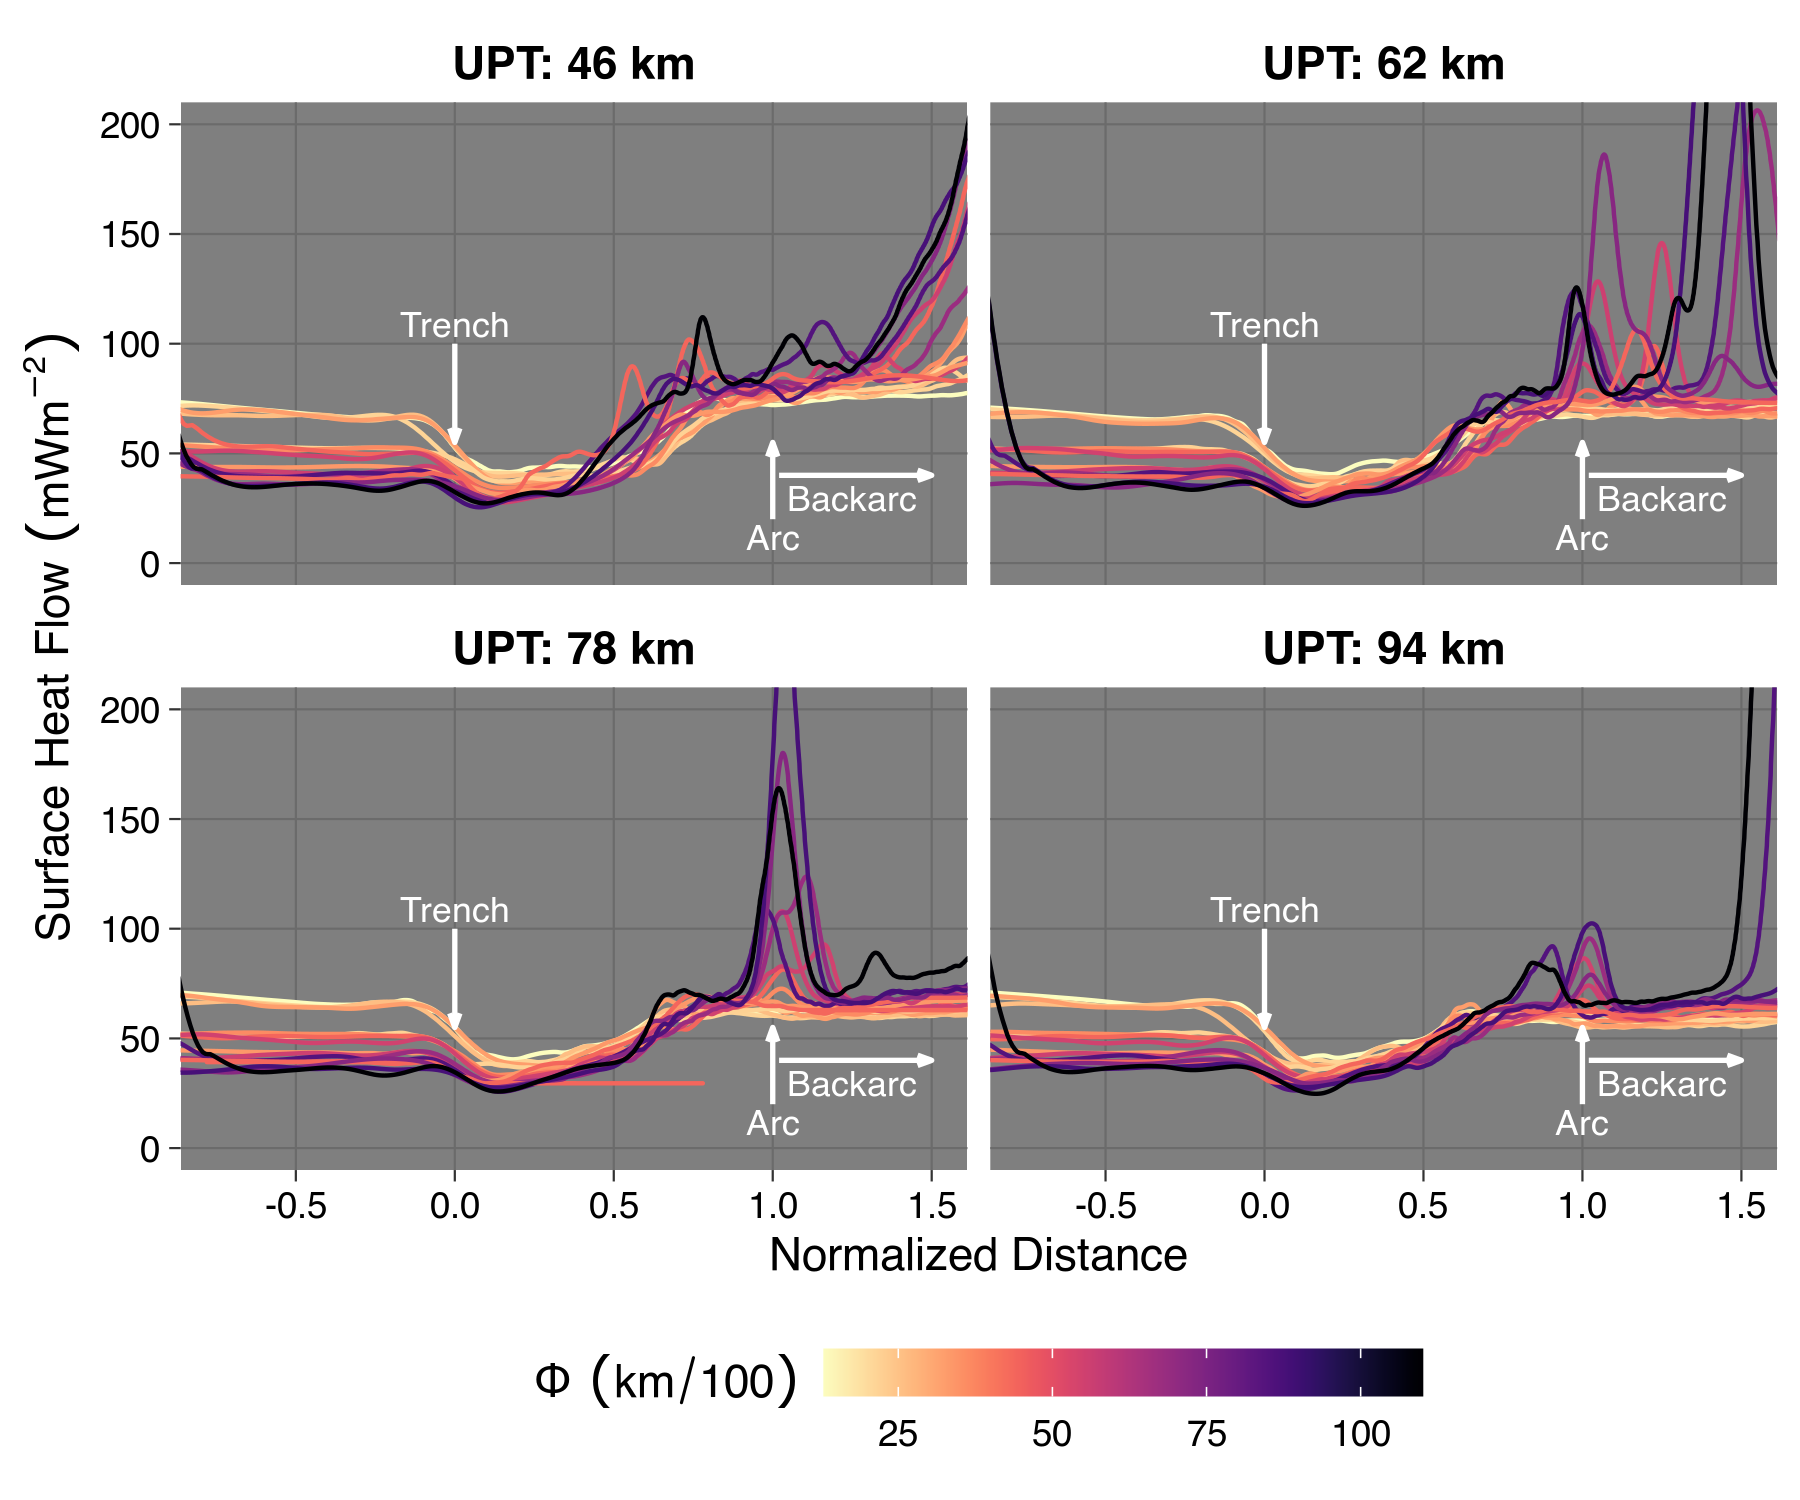
\includegraphics[width=1\linewidth,]{assets/figs/chpt2/figA7} 

}

\caption[Surface heat flow for all numerical experiments]{Surface heat flow calculated at approximately 10 $Ma$ for all numerical experiments. Normalized distance is the distance from the left boundary to the trench, divided by the distance between the trench and arc. Grayscale corresponds to $\Phi$. High amplitude fluctuations near the arc region (normalized distance = 1.0) correspond to vertical migration of fluids and melts. In the backarc region (normalized distance $\geq$ 1.0), these fluctuations correspond to lithospheric extension. Backarc extension is most apparent for high-$\Phi$ experiments (lighter gray lines). Experiments with no extension show a tight distribution of surface heat flow in the backarc region (darker gray lines).}\label{fig:hf}
\end{figure}

\cleardoublepage

\markboth{Appendix: Chapter 3}{Appendix: Chapter 3}

\hypertarget{section-1}{%
\chapter{}\label{section-1}}

\hypertarget{krigeOpt}{%
\section{Kriging System and Optimization}\label{krigeOpt}}

\hypertarget{ordinary-kriging}{%
\subsection{Ordinary Kriging}\label{ordinary-kriging}}

This study applies isotropic ordinary Kriging methods under the following general assumptions:

\begin{itemize}
\tightlist
\item
  \(\hat{\gamma}(h)\) is directionally invariant (isotropic)
\item
  \(\hat{\gamma}(h)\) is evaluated in two-dimensions and neglects elevation
\item
  The first and second moments of \(Z(u)\) are assumed to follow the conditions:
\end{itemize}

\begin{equation}
  \begin{aligned}
    &E[Z(u)] = \hat{Z}(u) = constant \\
    &E[(Z(u + h) - \hat{Z}(u))(Z(u) - \hat{Z}(u))] = C(h)
  \end{aligned}
  \label{eq:krigeAssumptions}
\end{equation}
\DIFdelbegin %DIFDELCMD < 

%DIFDELCMD < %%%
\DIFdelend where \(h\) is the lag distance, \(C(h)\) is the covariance function, \(E[Z(u)]\) is the expected value of the random variable \(Z(u)\), and \(\hat{Z}(u)\) is the arithmetic mean of \(Z(u)\).

Equation \eqref{eq:krigeAssumptions} is known as ``weak second-order stationarity''. It assumes the underlying probability distribution of the observations \(Z(u)\) does not change in space and the covariance \(C(h)\) only depends on the distance \(h\) between two observations. These assumptions are expected to be valid in cases where the underlying natural process is stochastic, spatially continuous, and has the property of additivity such that \(\frac{1}{n}\sum_{i=1}^n Z(u_i)\) has the same meaning as \(Z(u)\) (\protect\hyperlink{ref-bardossy1997}{Bárdossy, 1997}).

The following are two illustrative cases where Equation \eqref{eq:krigeAssumptions} is likely valid:

\begin{quote}
The thickness of a sedimentary unit with a homogeneous concentration of radioactive elements can be approximated by \(q_s = q_b + \int A \,dz\), where \(q_b\) is a constant heat flux entering the bottom of the layer and \(A\) is the heat production within the layer with thickness \(z\) (\protect\hyperlink{ref-furlong2013}{Furlong \& Chapman, 2013}). If one has two samples, \(Z(u_1) = 31~mW/m^2\) and \(Z(u_2) = 30.5~mW/m^2\), their corresponding thicknesses would be \(Z'(u_1) = 1000~m\) and \(Z'(u_2) = 500~m\) for \(A = 0.001~mW/m^3\) and \(q_b = 30~mW/m^2\). The variable, \(Z(u)\), in this case is additive because the arithmetic mean of the samples is a good approximation of the average sedimentary layer thickness, \((Z(u_1) + Z(u_2)) / 2 = 750~m\).
\end{quote}

\begin{quote}
The age of young oceanic lithosphere can be approximated by \(q_s(t) = kT_b(\pi\kappa t)^{-1/2}\), where \(q_s(t)\) is surface heat flow of a plate with age, \(t\), \(T_b\) is the temperature at the base of the plate, \(k\) is thermal conductivity, and \(\kappa = k/\rho C_p\) is thermal diffusivity (\protect\hyperlink{ref-stein1992}{Stein \& Stein, 1992}). Using reasonable values for \(k = 3.138~W/mK\), \(\rho = 3330~kg/m^3\), \(C_p = 1171~J/kgK\), \(T_b = 1350^{\circ}C\), two samples, \(Z(u_1) = 180~mW/m^2\) and \(Z(u_2) = 190~mW/m^2\), would correspond to plates with ages of \(Z'(u_1) = 10~Ma\), and \(Z'(u_2) = 9~Ma\), respectively. Since \(Z(u_1) + Z(u_2) / 2 = 185~mW/m^2\) and \(Z'(185~mW/m^2) = 9.5~Ma = Z'(u_1) + Z'(u_2) / 2\), the variable \(Z(u)\) in this case is also additive.
\end{quote}

Equation \eqref{eq:krigeAssumptions} is likely invalid in regions that transition among two or more tectonic regimes, however. For example, the expected (mean) heat flow \(E[Z(u)]\) will change when moving from a spreading center to a subduction zone and thus \(E[Z(u)] \neq constant\) over the region of interest. In other words, stationarity is violated and Kriging estimates will become spurious.

The second step is fitting a variogram model \(\gamma(h)\) to the experimental variogram. This study fits six popular variogram models with sills (or theoretical sills) to the experimental variogram. The models are defined as (\protect\hyperlink{ref-pebesma2004}{Pebesma, 2004}):
\DIFdelbegin %DIFDELCMD < 

%DIFDELCMD < %%%
\DIFdelend \begin{equation}
  \begin{aligned}
    Bes &\leftarrow \gamma(h) = 1 - \frac{h}{a}\ K_1\left(\frac{h}{a}\right) \quad \text{for } \  h \geq 0 \\
    Cir &\leftarrow \gamma(h) =
    \begin{cases}
      \frac{2}{\pi}\frac{h}{a}\ \sqrt{1-\left(\frac{h}{a}\right)^2} + \frac{2}{\pi}\ arcsin\left(\frac{h}{a}\right) \quad \text{for } \  0 \leq h \leq a \\
      n + s \quad \text{for } \  h > a
    \end{cases} \\
    Exp &\leftarrow \gamma(h) = 1 - exp\left(\frac{-h}{a}\right) \quad \text{for } \  h \geq 0 \\
    Gau &\leftarrow \gamma(h) = 1 - exp\left(\left[\frac{-h}{a}\right]^2\right) \quad \text{for } \  h \geq 0 \\
    Lin &\leftarrow \gamma(h) =
    \begin{cases}
      \frac{h}{a} \quad \text{for } \  0 \leq h \leq a \\
      n + s \quad \text{for } \  h > a
    \end{cases} \\
    Sph &\leftarrow \gamma(h) =
    \begin{cases}
      \frac{3}{2}\frac{h}{a} - \frac{1}{2}\left(\frac{h}{a}\right)^3 \quad \text{for } \  0 \leq h \leq a \\
      n + s \quad \text{for } \  h > a
    \end{cases} \\
  \end{aligned}
  \label{eq:varMods}
\end{equation}
\DIFdelbegin %DIFDELCMD < 

%DIFDELCMD < %%%
\DIFdelend where \(n\) is the nugget, \(s\) is the sill, \(a\) is the effective range, \(K_1\) is a modified Bessel function. The models are Bessel, Circular, Exponential, Gaussian, Linear, and Spherical. For models without explicit sills (Bes, Exp, Gau), the effective range \(a\) is the distance where the variogram reaches 95\% of its maximum defined as 4\(a\), 3\(a\), and \(\sqrt{3}a\) for Bes, Exp, and Gau, respectively (\protect\hyperlink{ref-graler2016}{Gräler et al., 2016}; \protect\hyperlink{ref-pebesma2004}{Pebesma, 2004}). The function \texttt{fit.variogram} in \texttt{gstat} is used to try all variogram models. The best model is selected by the minimum weighted least squares (\protect\hyperlink{ref-pebesma2004}{Pebesma, 2004}) error with weights proportional to the number of points in each lag divided by the squared lag distance \(wt = N(h)_k/h_k^2)\).

Ordinary Kriging is used for interpolation, which estimates unknown observations \(\hat{Z}(u)\) as a linear combination of all known observations (\protect\hyperlink{ref-bardossy1997}{Bárdossy, 1997}):
\DIFdelbegin %DIFDELCMD < 

%DIFDELCMD < %%%
\DIFdelend \begin{equation}
  \hat{Z}(u) = \sum_{i=1}^n \lambda_i Z(u_i)
  \label{eq:linEstimate}
\end{equation}

The conditions in Equation \eqref{eq:krigeAssumptions} set up a constrained minimization problem that can be solved with a system of linear equations. The expected value of \(Z(u)\) is assumed to be the mean according to \eqref{eq:krigeAssumptions}, so the weights must be:
\DIFdelbegin %DIFDELCMD < 

%DIFDELCMD < %%%
\DIFdelend \begin{equation}
  \begin{aligned}
    E[\hat{Z}(u)] &= \sum_{i=1}^n \lambda_i E[Z(u_i)] \\
    \sum_{i=1}^n \lambda_i &= 1
  \end{aligned}
  \label{eq:unbiased}
\end{equation}

This constraint is known as the unbiased condition, which states that the sum of the weights must equal one. However, there is an infinite set of real numbers one could use for the weights, \(\lambda_i\). The goal is to find the set of weights in Equation \eqref{eq:linEstimate} that minimizes the estimation variance. This can be solved by minimizing the covariance function, \(C(h)\) from Equation \eqref{eq:krigeAssumptions}:
\DIFdelbegin %DIFDELCMD < 

%DIFDELCMD < %%%
\DIFdelend \begin{equation}
  \begin{aligned}
    & \sigma^2(u) = Var[Z(u) - \hat{Z}(u)] = \\
    & E\left[(Z(u) - \sum_{i=1}^n \lambda_i Z(u_i))^2\right] = \\
    & E\left[Z(u)^2 + \sum_{j=1}^n \sum_{i=1}^n \lambda_j \lambda_i Z(u_j)Z(u_i) - 2 \sum_{i=1}^n \lambda_i Z(u_i)Z(u)\right] = \\
    & C(0) + \sum_{j=1}^n \sum_{i=1}^n \lambda_j \lambda_i C(u_i - u_j) - 2 \sum_{i=1}^n \lambda_i C(u_i - u)
  \end{aligned}
  \label{eq:minVar}
\end{equation}

Minimizing Equation \eqref{eq:minVar} with respect to the unbiased condition (Equation \eqref{eq:unbiased}), yields the best linear unbiased estimator (BLUE, \protect\hyperlink{ref-bardossy1997}{Bárdossy, 1997}) for Equation \eqref{eq:linEstimate} and together comprise the Kriging system of equations. The functions \texttt{krige} and \texttt{krige.cv} in \texttt{gstat} are used for surface heat flow interpolation and error estimation by k-fold cross-validation (\protect\hyperlink{ref-pebesma2004}{Pebesma, 2004}).

\hypertarget{nloptr}{%
\subsection{\texorpdfstring{Optimization with \texttt{nloptr}}{Optimization with nloptr}}\label{nloptr}}

Achieving accurate Kriging results depends on one's choice of many Kriging parameters, \(\Theta\). In this study, we investigate a set of parameters:
\DIFdelbegin %DIFDELCMD < 

%DIFDELCMD < %%%
\DIFdelend \begin{equation} 
  \Theta = \{model,\ n,\ c,\ n_{max},\ l\}
  \label{eq:params}
\end{equation}
\DIFdelbegin %DIFDELCMD < 

%DIFDELCMD < %%%
\DIFdelend where \(model\) is one of the variogram models defined in Equation \eqref{eq:varMods}, \(n\) is the number of lags, \(c\) is a lag cutoff proportionality constant, \(n_{max}\) is the maximum point-pairs for local Kriging, and \(l\) is a horizontal lag shift constant. The lag cutoff constant \(c\) controls the maximum separation distance between pairs of points used to calculate the experimental variogram (i.e.~the x-axis range or ``width'' of the experimental variogram). The horizontal lag shift constant \(l\) removes the first few lags from being evaluated by effectively shifting all lags to the left proportionally by \(l\). This is necessary to avoid negative ranges when fitting experimental variograms with anomalously high variances at small lag distances.

The goal is to find \(\Theta\) such that the Kriging function \(f(x_i;\ \Theta)\) gives the minimum error defined by a cost function \(C(\Theta)\), which represents the overall goodness of fit of the interpolation. This study defines a cost function that simultaneously considers errors between the experimental variogram \(\hat{\gamma}(h)\) and modelled variogram \(\gamma(h)\), and between surface heat flow observations \(Z(u_i)\) and Kriging estimates \(\hat{Z}(u)\) (after \protect\hyperlink{ref-li2018}{Li et al., 2018}):
\DIFdelbegin %DIFDELCMD < 

%DIFDELCMD < %%%
\DIFdelend \begin{equation}
  \begin{aligned}
    C(\Theta) &= w_{vgrm}\ C_{vgrm}(\Theta) + w_{interp}\ C_{interp}(\Theta) \\
    &w_{vgrm} + w_{interp} = 1
  \end{aligned}
  \label{eq:cost}
\end{equation}
\DIFdelbegin %DIFDELCMD < 

%DIFDELCMD < %%%
\DIFdelend where \(C_{vgrm}(\Theta)\) is the normalized \glsfirst{rmse} evaluated during variogram fitting and \(C_{interp}(\Theta)\) is the normalized \gls{rmse} evaluated during Kriging. Weighted ordinary least squares is used to evaluate \(C_{vgrm}(\Theta)\), whereas k-fold cross-validation is used to evaluate \(C_{interp}(\Theta)\). K-fold splits the dataset \(|Z(u_i)|\) into \(k\) equal intervals, removes observations from an interval, and then estimates the removed observations by fitting a variogram model to data in the remaining \(k-1\) intervals. This process is repeated over all \(k\) intervals so that the whole dataset has been cross-validated. The final expression to minimize becomes:
\DIFdelbegin %DIFDELCMD < 

%DIFDELCMD < %%%
\DIFdelend \begin{equation}
  \begin{aligned}
    &C(\Theta) = \\
    &\frac{w_{vgrm}}{\sigma_{vgrm}}\ \left(\frac{1}{N(h)}\ \sum_{k=1}^{N}\ w(h_k)\ [\hat{\gamma}(h_k)-\gamma(h_k;\ \Theta)]^2\right)^{1/4} + \\
    &\frac{w_{interp}}{\sigma_{interp}}\ \left(\frac{1}{M}\ \sum_{i=1}^{M}\ [Z(u_i)-\hat{Z}(u_i;\ \Theta)]^2\right)^{1/2}
  \end{aligned}
  \label{eq:costExp}
\end{equation}
\DIFdelbegin %DIFDELCMD < 

%DIFDELCMD < %%%
\DIFdelend where \(N(h)\) is the number of point-pairs used to evaluate the experimental variogram and \(w(h_k) = N(h)_k/h_k^2\) are weights defining the importance of the \(kth\) lag on the variogram model fit. \(Z(u_i)\) and \(\hat{Z}(u_i;\ \Theta)\) are the observed and estimated values, respectively, and \(M\) is the number of measurements in \(|Z(u_i)|\). The \glspl{rmse} are normalized by dividing by \(\sigma_{vgrm}\) and \(\sigma_{interp}\), which represent the standard deviation of the experimental variogram \(\hat{\gamma}(h)\) and surface heat flow observations \(Z(u_i)\), respectively. The weights \(w_{vgrm}\) and \(w_{interp}\) were varied between 0 and 1 to test the effects on \(C(\Theta)\). Preferred weights of \(w_{vgrm}\) = \(w_{interp}\) = 0.5 are selected to balance the effects of \(C_{vgrm}(\Theta)\) and \(C_{interp}(\Theta)\) on the cost function.

\DIFdelbegin %DIFDELCMD < \begin{table}
%DIFDELCMD < 

%DIFDELCMD < %%%
%DIFDELCMD < \caption{%
{%DIFAUXCMD
%DIFDELCMD < \label{tab:nloptrBounds}%%%
\DIFdelFL{Search bounds for nloptr minimization}}
%DIFAUXCMD
%DIFDELCMD < \centering
%DIFDELCMD < \begin{tabular}[t]{lll}
%DIFDELCMD < \toprule
%DIFDELCMD < %%%
\DIFdelFL{Parameter }%DIFDELCMD < & %%%
\DIFdelFL{Lower }%DIFDELCMD < & %%%
\DIFdelFL{Upper}%DIFDELCMD < \\
%DIFDELCMD < \midrule
%DIFDELCMD < \cellcolor{gray!6}{Lag cutoff (c)} & \cellcolor{gray!6}{1} & \cellcolor{gray!6}{20}\\
%DIFDELCMD < %%%
\DIFdelFL{Lag number (n) }%DIFDELCMD < & %%%
\DIFdelFL{15 }%DIFDELCMD < & %%%
\DIFdelFL{50}%DIFDELCMD < \\
%DIFDELCMD < \cellcolor{gray!6}{Lag shift (l)} & \cellcolor{gray!6}{1} & \cellcolor{gray!6}{10}\\
%DIFDELCMD < %%%
\DIFdelFL{Max local pairs ($n_{max}$) }%DIFDELCMD < & %%%
\DIFdelFL{10 }%DIFDELCMD < & %%%
\DIFdelFL{50}%DIFDELCMD < \\
%DIFDELCMD < \bottomrule
%DIFDELCMD < \end{tabular}
%DIFDELCMD < \end{table}
%DIFDELCMD < 

%DIFDELCMD < %%%
\DIFdelend \begin{figure}[htbp]

{\centering 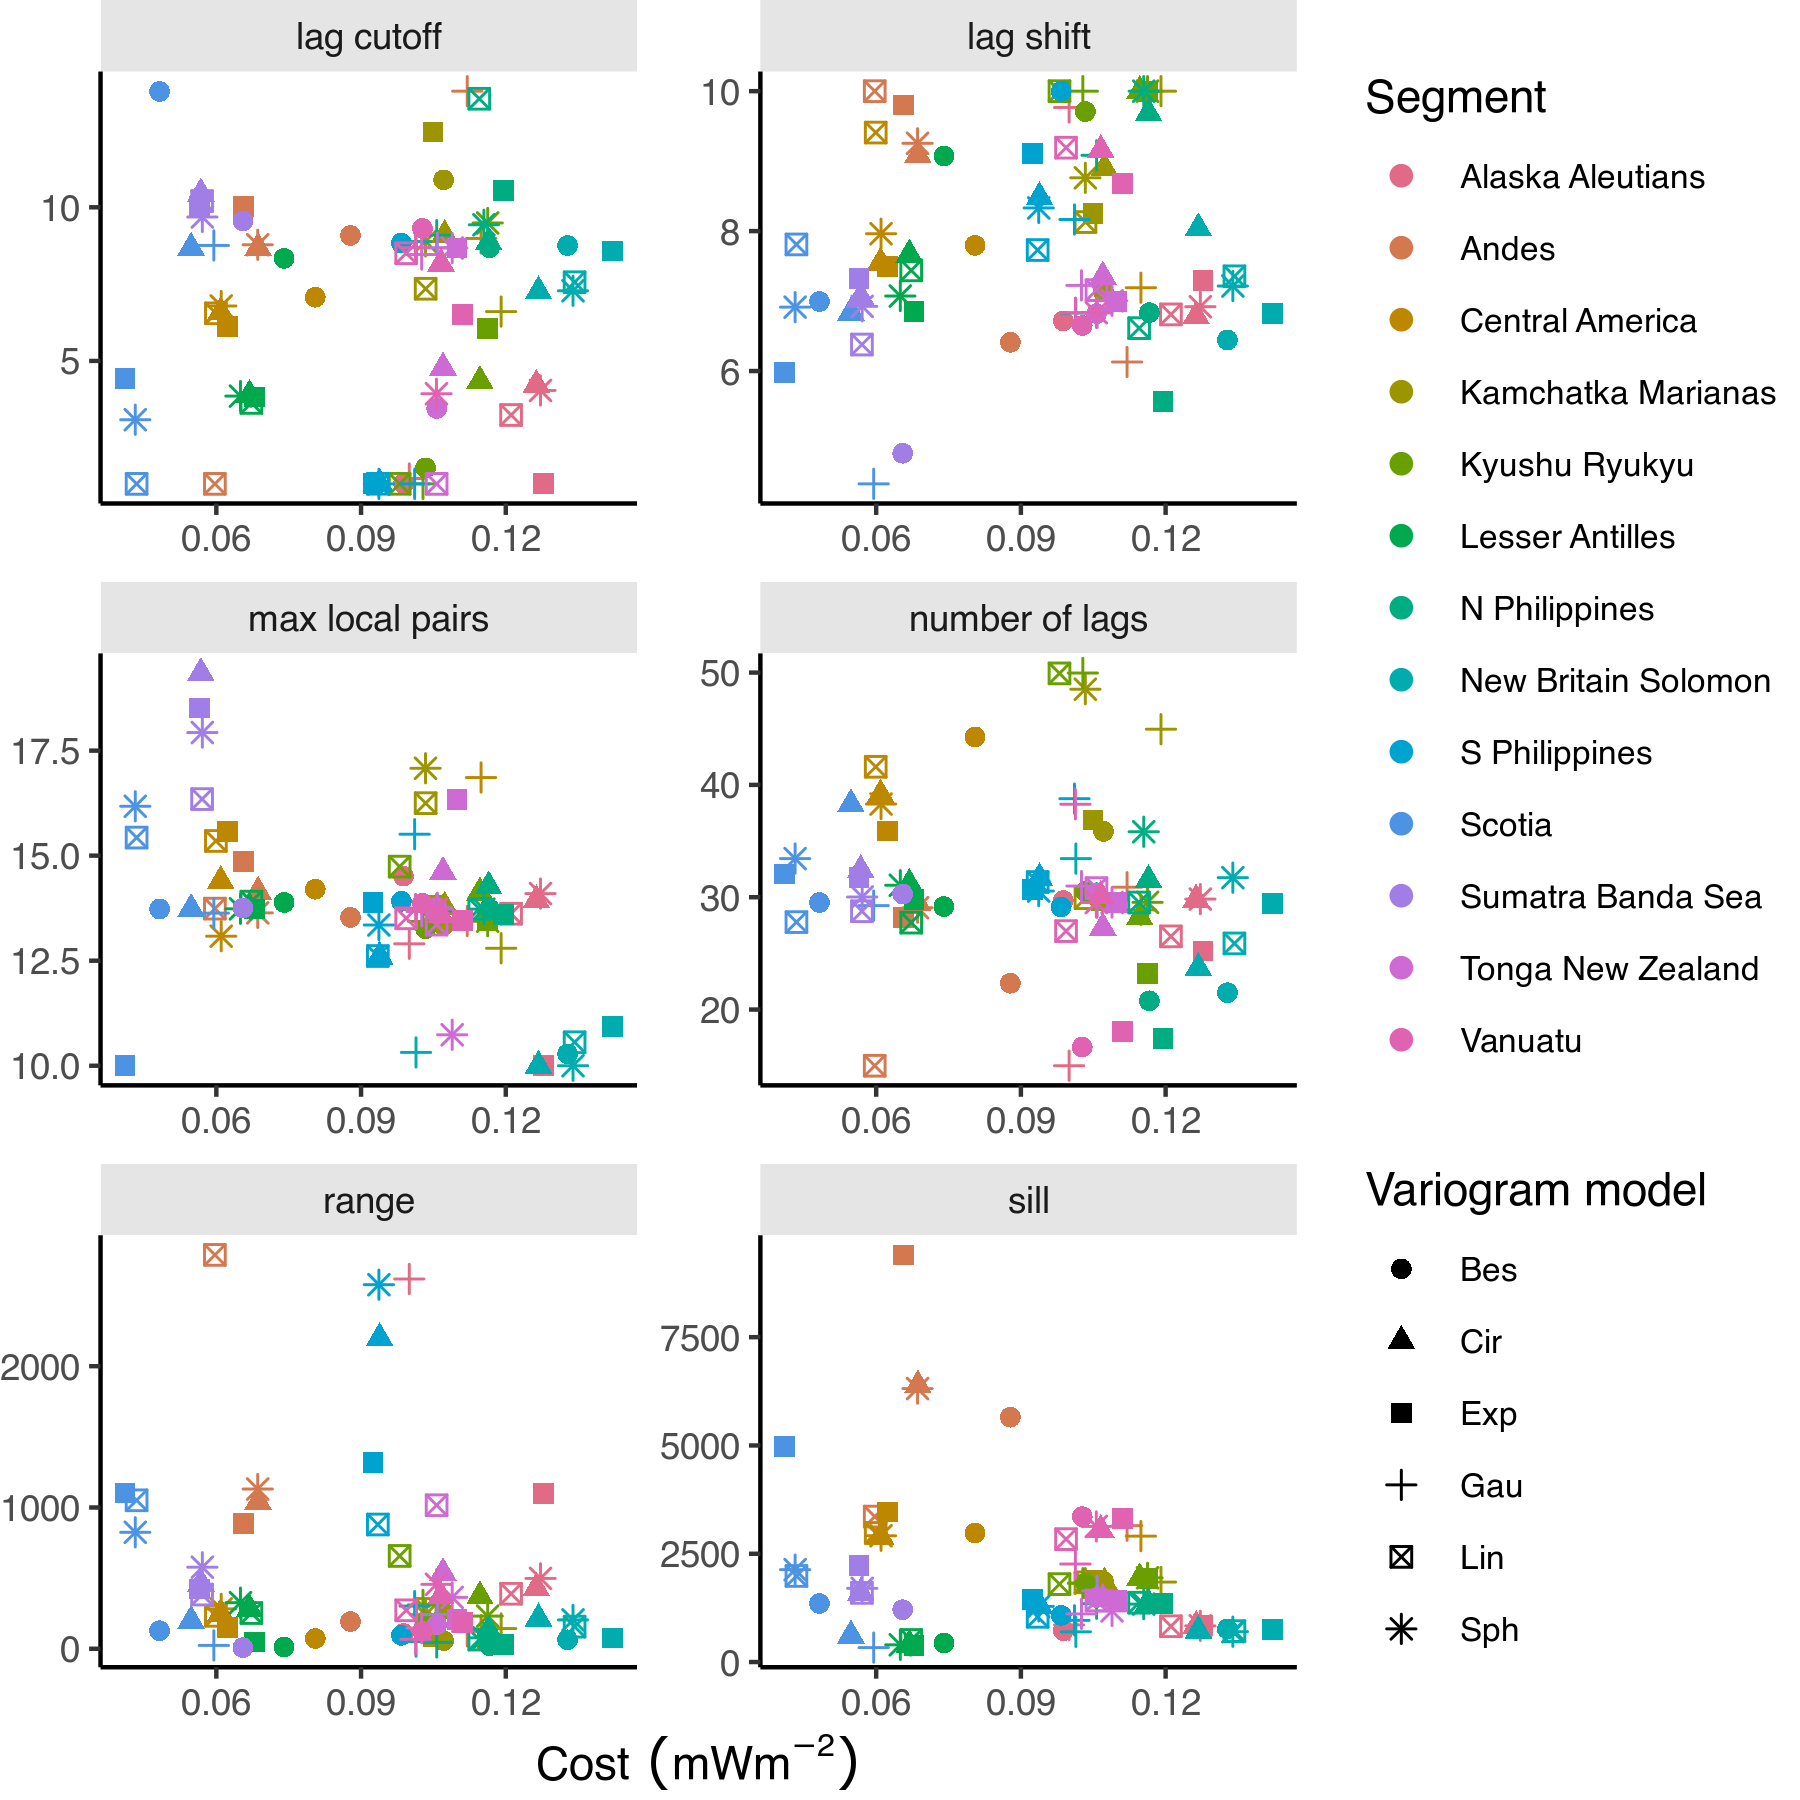
\includegraphics[width=1\linewidth,]{assets/figs/chpt3/vgrmSummary} 

}

\caption[Summary of optimized variogram models]{Summary of optimized Kriging parameters. Cost does not correlate with Kriging parameters (with a possible exception of variogram sills), indicating the optimization procedure is successfully generalizeable across subduction zone segments.}\label{fig:vgrmSummaryPlot}
\end{figure}

Minimization of \(C(\Theta)\) is achieved by non-linear constrained optimization using algorithms defined in the \texttt{R} package \texttt{nloptr} (\protect\hyperlink{ref-ypma2014}{Ypma, 2014})\DIFdelbegin \DIFdel{with bounds in Table \ref{tab:nloptrBounds}}\DIFdelend . Both global and local search methods were applied with similar success. Please see \href{https://nlopt.readthedocs.io/en/latest/NLopt_Introduction/}{the official documentation} for more information on \texttt{nloptr} and available optimization algorithms. The run used to produce the visualizations in Chapter \ref{chpt3} uses the \texttt{NLOPT\_LN\_BOBYQA} option with 50 max iterations, \DIFaddbegin \DIFadd{leave-one-out }\DIFaddend cross-validation \DIFdelbegin \DIFdel{with k-folds equal to half of }\DIFdelend \DIFaddbegin \DIFadd{(k-fold \(=\) }\DIFaddend the number of observations\DIFaddbegin \DIFadd{) }\DIFaddend in the evaluated segment, and cost function weights of \(w_{vgrm}\) = \(w_{interp}\) = 0.5 (Figure \ref{fig:optTrace}). All data, code, and instructions to reproduce results in this chapter can be found at \url{https://github.com/buchanankerswell/kerswell_kohn_backarc}.



\begin{figure}[htbp]

{\centering 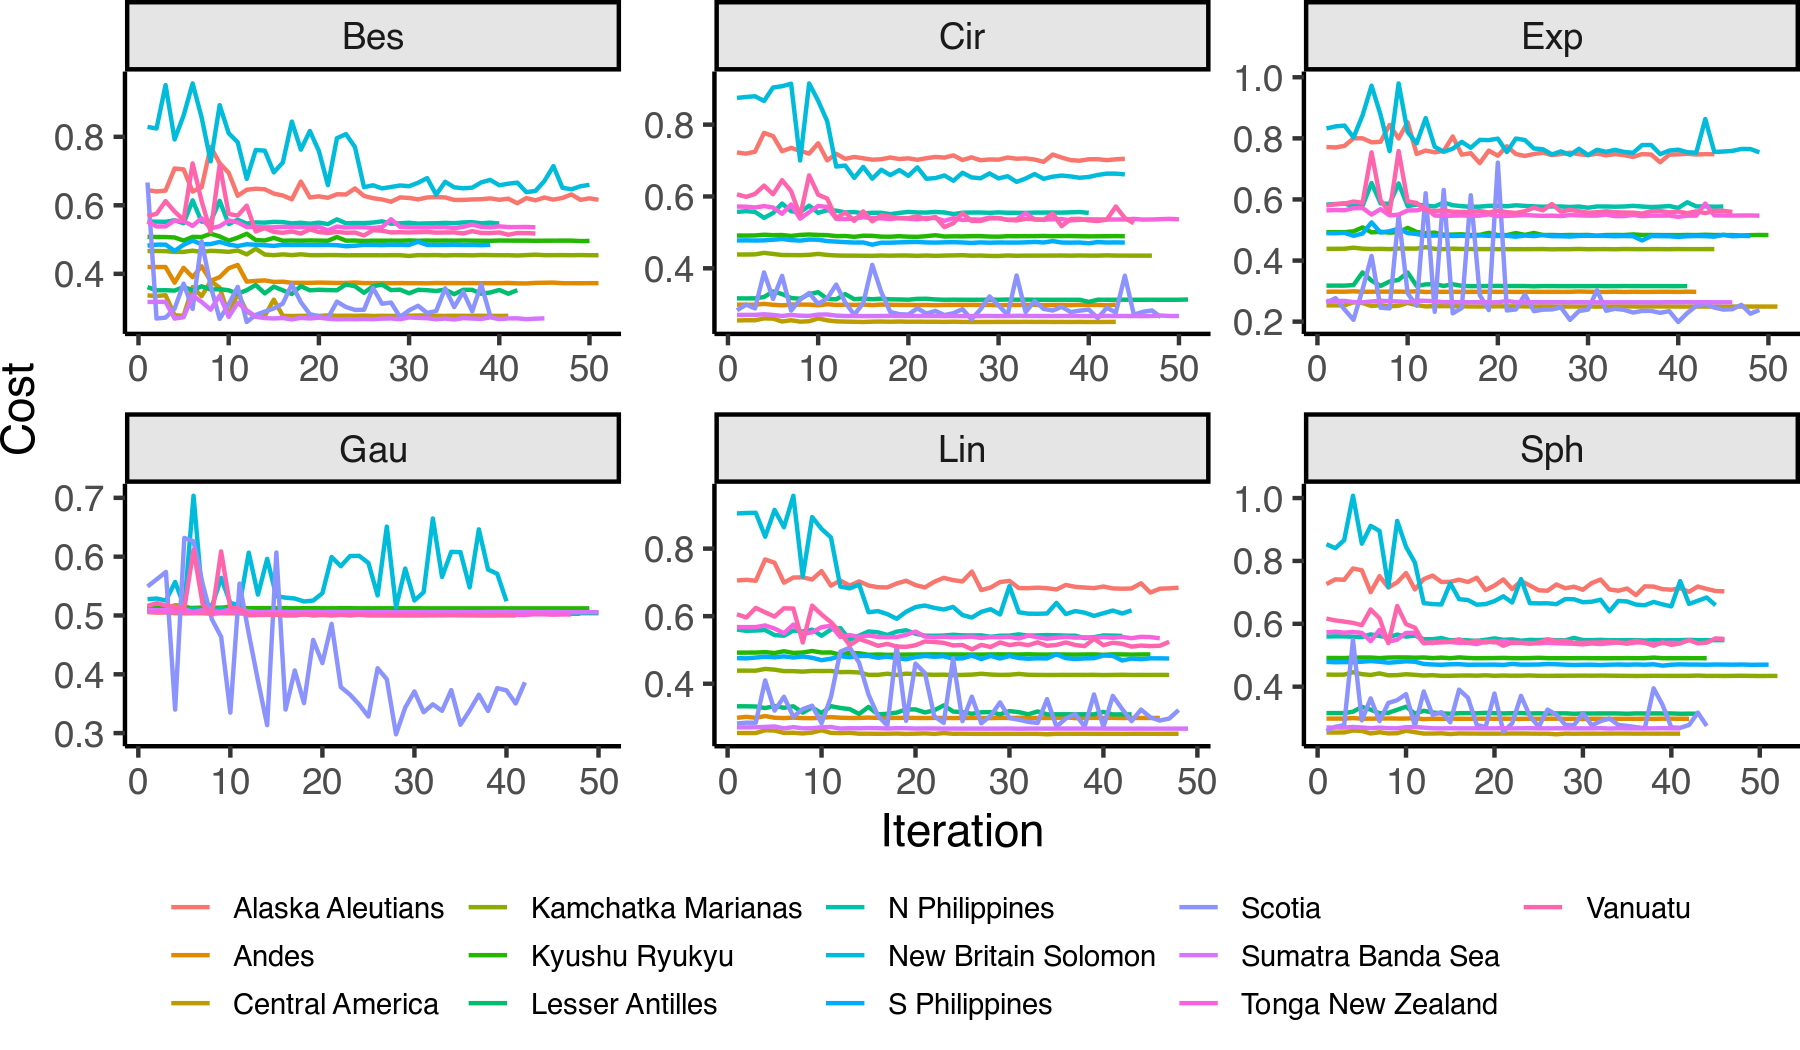
\includegraphics[width=1\linewidth,]{assets/figs/chpt3/optTrace} 

}

\caption[Cost function minimization for Kriging interpolations]{Cost function minimization for Kriging interpolations presented in Chapter \ref{chpt3}. Most variogram models (panels) converge on a local optimum for most Kriging domains (lines) after 15-20 iterations. Each line represents one of thirteen subduction zone segments. Gaussian models are the least stable and produce spurious results. See text for bound constraints and other options.}\label{fig:optTrace}
\end{figure}

\DIFaddbegin \clearpage

\hypertarget{thermoglobe-summary}{%
\section{ThermoGlobe Summary}\label{thermoglobe-summary}}



\begin{figure}[htbp]

{\centering 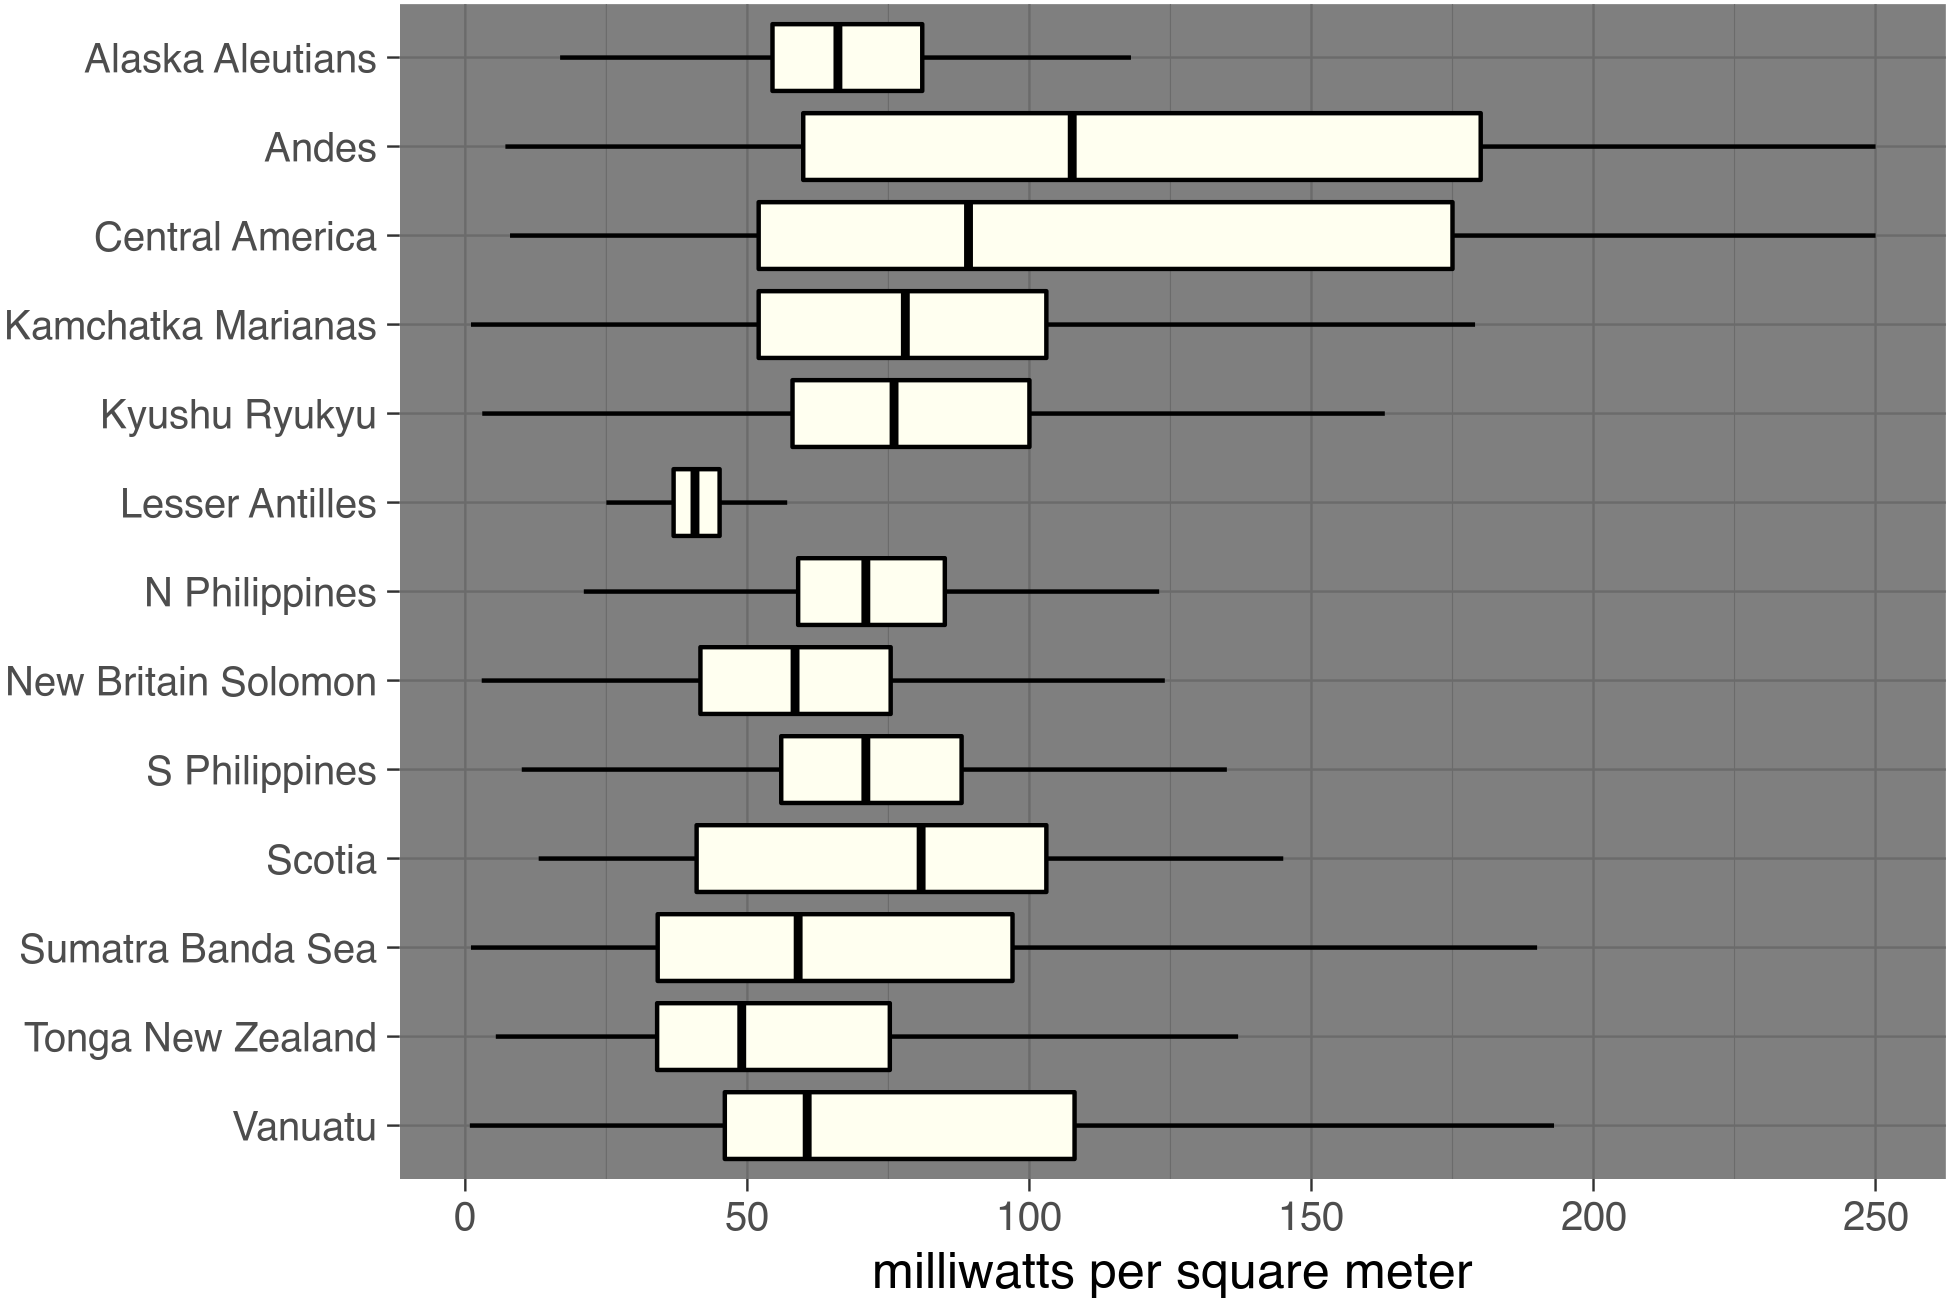
\includegraphics[width=1\linewidth,]{assets/figs/chpt3/hfSummary} 

}

\caption[Distributions of ThermoGlobe observations near 13 active subduction zone segments]{\DIFaddFL{Distribution of ThermoGlobe observations from Lucazeau (}\protect\hyperlink{ref-lucazeau2019}{2019}\DIFaddFL{) cropped within 1000 \(km\)-radius circular buffers around 13 active subduction zone segments. Heat flow distributions are centered between 41 and 108 \(mWm^{-2}\) and highly right-skewed. Skewness represents near-surface perturbations from geothermal systems and tectonic regions with high thermal activity. Complex heat exchange between tectonic and near-surface processes is apparent from the broad, irregular surface heat flow distributions. Distributions are colored by quartiles (25\%, 50\%, 75\%).}}\label{fig:hfSummaryPlot}
\end{figure}

\begin{table}

\caption{\label{tab:hfSummaryTable}\DIFaddFL{ThermoGlobe heat flow summary by segment}}
\centering
\begin{threeparttable}
\begin{tabular}[t]{lrrrrrrr}
\toprule
\DIFaddFL{Segment }& \DIFaddFL{n }& \DIFaddFL{Min }& \DIFaddFL{Max }& \DIFaddFL{Median }& \DIFaddFL{IQR }& \DIFaddFL{Mean }& \DIFaddFL{$\sigma$}\\
\midrule
\cellcolor{gray!6}{Alaska Aleutians} & \cellcolor{gray!6}{290} & \cellcolor{gray!6}{6} & \cellcolor{gray!6}{196} & \cellcolor{gray!6}{66} & \cellcolor{gray!6}{27} & \cellcolor{gray!6}{71} & \cellcolor{gray!6}{28}\\
\DIFaddFL{Andes }& \DIFaddFL{1398 }& \DIFaddFL{7 }& \DIFaddFL{250 }& \DIFaddFL{108 }& \DIFaddFL{120 }& \DIFaddFL{119 }& \DIFaddFL{66}\\
\cellcolor{gray!6}{Central America} & \cellcolor{gray!6}{1443} & \cellcolor{gray!6}{8} & \cellcolor{gray!6}{250} & \cellcolor{gray!6}{89} & \cellcolor{gray!6}{123} & \cellcolor{gray!6}{110} & \cellcolor{gray!6}{67}\\
\DIFaddFL{Kamchatka Marianas }& \DIFaddFL{2269 }& \DIFaddFL{1 }& \DIFaddFL{248 }& \DIFaddFL{78 }& \DIFaddFL{51 }& \DIFaddFL{83 }& \DIFaddFL{42}\\
\cellcolor{gray!6}{Kyushu Ryukyu} & \cellcolor{gray!6}{1895} & \cellcolor{gray!6}{3} & \cellcolor{gray!6}{250} & \cellcolor{gray!6}{76} & \cellcolor{gray!6}{42} & \cellcolor{gray!6}{84} & \cellcolor{gray!6}{42}\\
\DIFaddFL{Lesser Antilles }& \DIFaddFL{3010 }& \DIFaddFL{13 }& \DIFaddFL{242 }& \DIFaddFL{41 }& \DIFaddFL{8 }& \DIFaddFL{46 }& \DIFaddFL{18}\\
\cellcolor{gray!6}{N Philippines} & \cellcolor{gray!6}{568} & \cellcolor{gray!6}{3} & \cellcolor{gray!6}{231} & \cellcolor{gray!6}{71} & \cellcolor{gray!6}{26} & \cellcolor{gray!6}{75} & \cellcolor{gray!6}{33}\\
\DIFaddFL{New Britain Solomon }& \DIFaddFL{101 }& \DIFaddFL{3 }& \DIFaddFL{143 }& \DIFaddFL{58 }& \DIFaddFL{34 }& \DIFaddFL{61 }& \DIFaddFL{26}\\
\cellcolor{gray!6}{S Philippines} & \cellcolor{gray!6}{460} & \cellcolor{gray!6}{1} & \cellcolor{gray!6}{224} & \cellcolor{gray!6}{71} & \cellcolor{gray!6}{32} & \cellcolor{gray!6}{74} & \cellcolor{gray!6}{34}\\
\DIFaddFL{Scotia }& \DIFaddFL{25 }& \DIFaddFL{13 }& \DIFaddFL{145 }& \DIFaddFL{81 }& \DIFaddFL{62 }& \DIFaddFL{79 }& \DIFaddFL{43}\\
\cellcolor{gray!6}{Sumatra Banda Sea} & \cellcolor{gray!6}{1418} & \cellcolor{gray!6}{1} & \cellcolor{gray!6}{247} & \cellcolor{gray!6}{59} & \cellcolor{gray!6}{63} & \cellcolor{gray!6}{68} & \cellcolor{gray!6}{42}\\
\DIFaddFL{Tonga New Zealand }& \DIFaddFL{354 }& \DIFaddFL{5 }& \DIFaddFL{218 }& \DIFaddFL{49 }& \DIFaddFL{40 }& \DIFaddFL{59 }& \DIFaddFL{37}\\
\cellcolor{gray!6}{Vanuatu} & \cellcolor{gray!6}{137} & \cellcolor{gray!6}{2} & \cellcolor{gray!6}{223} & \cellcolor{gray!6}{61} & \cellcolor{gray!6}{62} & \cellcolor{gray!6}{80} & \cellcolor{gray!6}{52}\\
\bottomrule
\end{tabular}
\begin{tablenotes}
\item \uline{\textit{key}}\DIFaddFL{: n: }[\DIFaddFL{\# of observations}]\DIFaddFL{, all other units are in $mWm^{-2}$
}\item \uline{\textit{note}}\DIFaddFL{: ThermoGlobe data are filtered for quality, restricted to }[\DIFaddFL{0, 250) $mWm^{-2}$, and cropped within 1000 $km$-radius circular buffers of segment boundaries
}\end{tablenotes}
\end{threeparttable}
\end{table}

\clearpage

\DIFaddend \hypertarget{vgrmModelsAppendix}{%
\section{Variogram Models}\label{vgrmModelsAppendix}}

Below are all \DIFdelbegin \DIFdel{variogram models fitted to experimental variograms }\DIFdelend \DIFaddbegin \DIFadd{fitted variogram models }\DIFaddend for each subduction zone segment. Please refer to Table \DIFdelbegin \DIFdel{\ref{tab:vgrmSummaryTable} }\DIFdelend \DIFaddbegin \DIFadd{\ref{tab:vgrmSummaryTableLong} }\DIFaddend for variogram parameters.

\begin{figure}
\centering
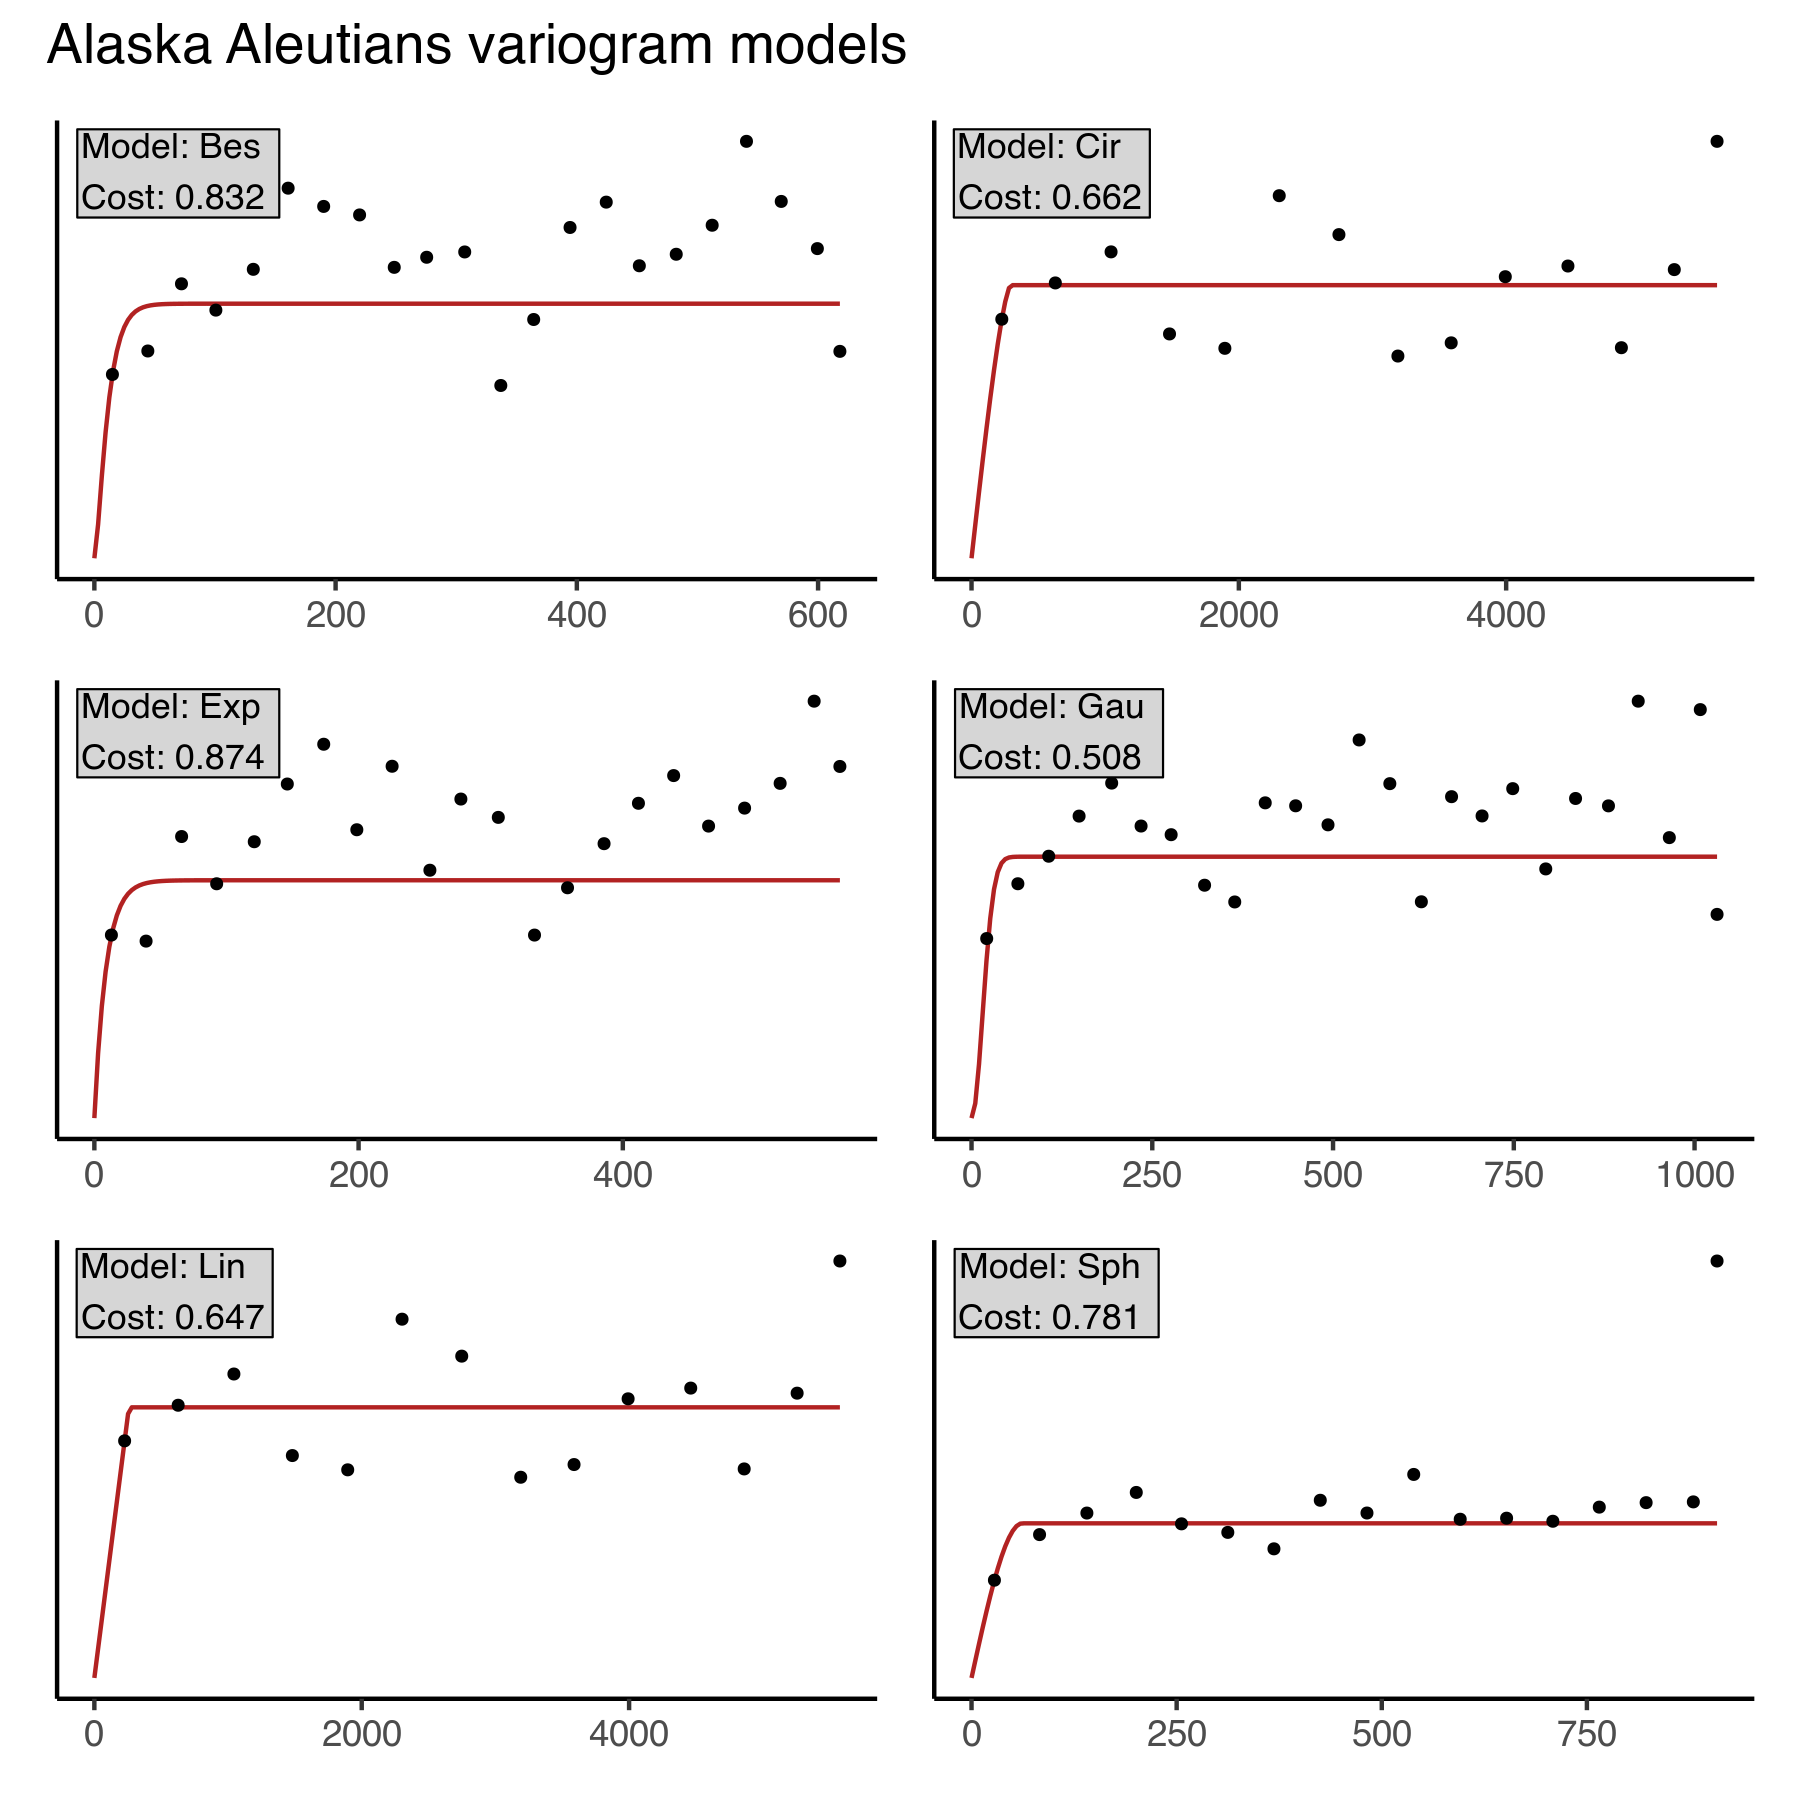
\includegraphics{assets/figs/chpt3/AlaskaAleutiansVgrms.png}
\caption[Fitted variograms for Alaska Aleutians]{Fitted variograms for Alaska Aleutians}
\end{figure}

\begin{figure}
\centering
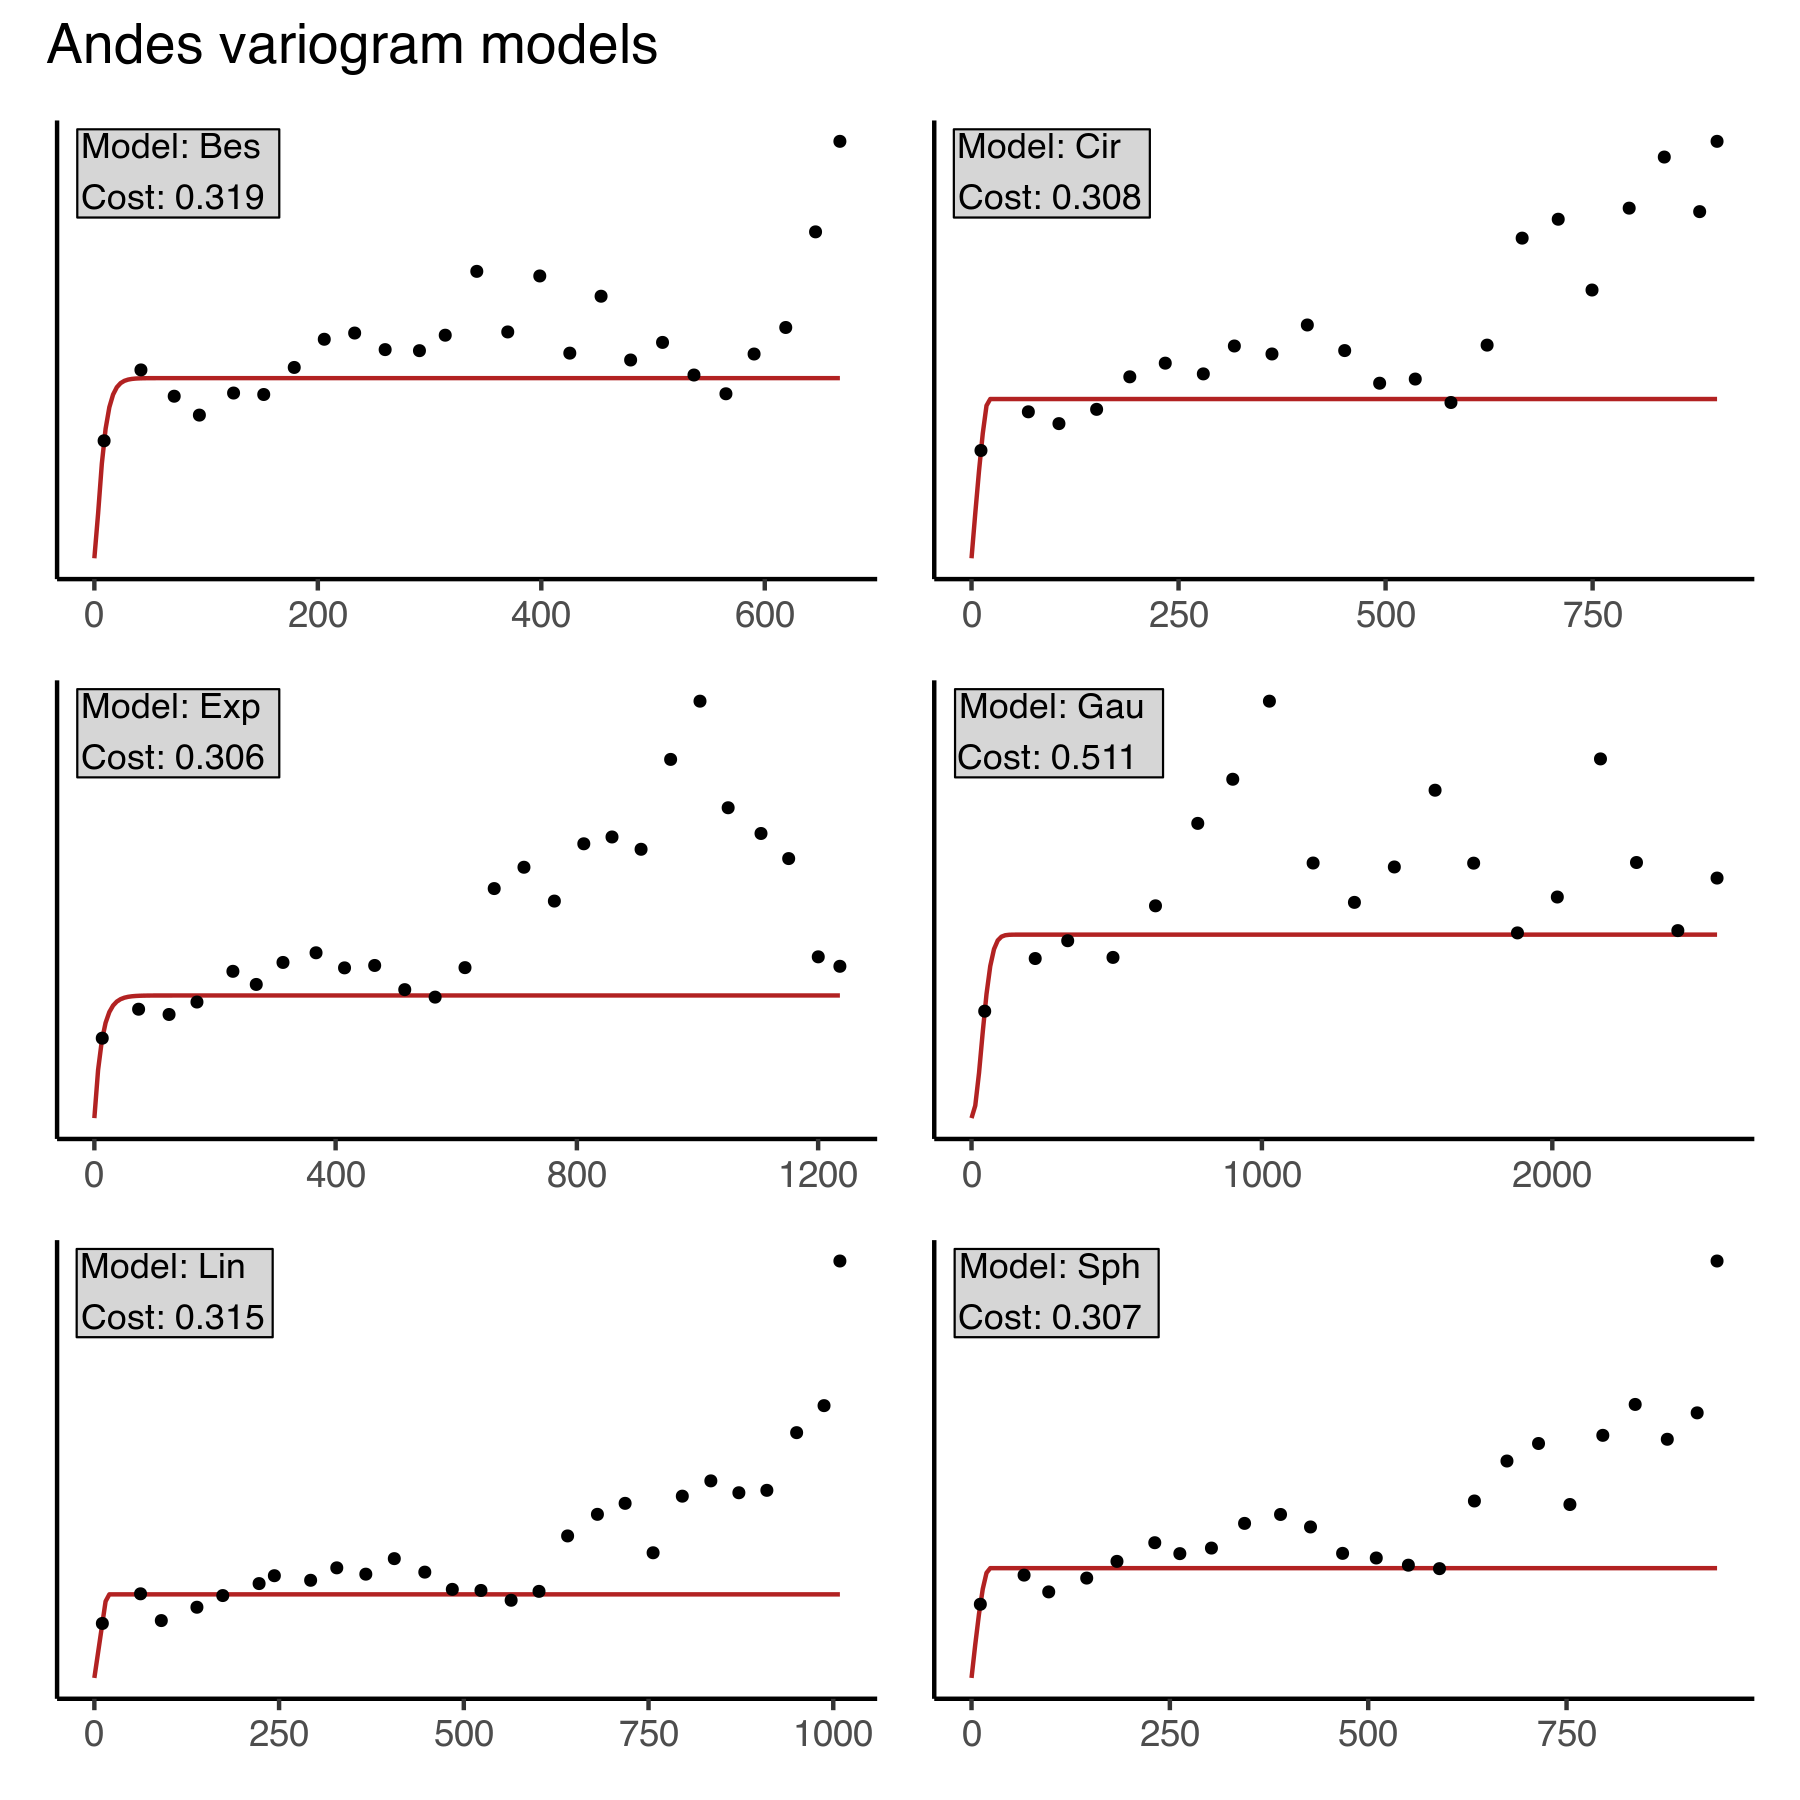
\includegraphics{assets/figs/chpt3/AndesVgrms.png}
\caption[Fitted variograms for Andes]{Fitted variograms for Andes}
\end{figure}

\begin{figure}
\centering
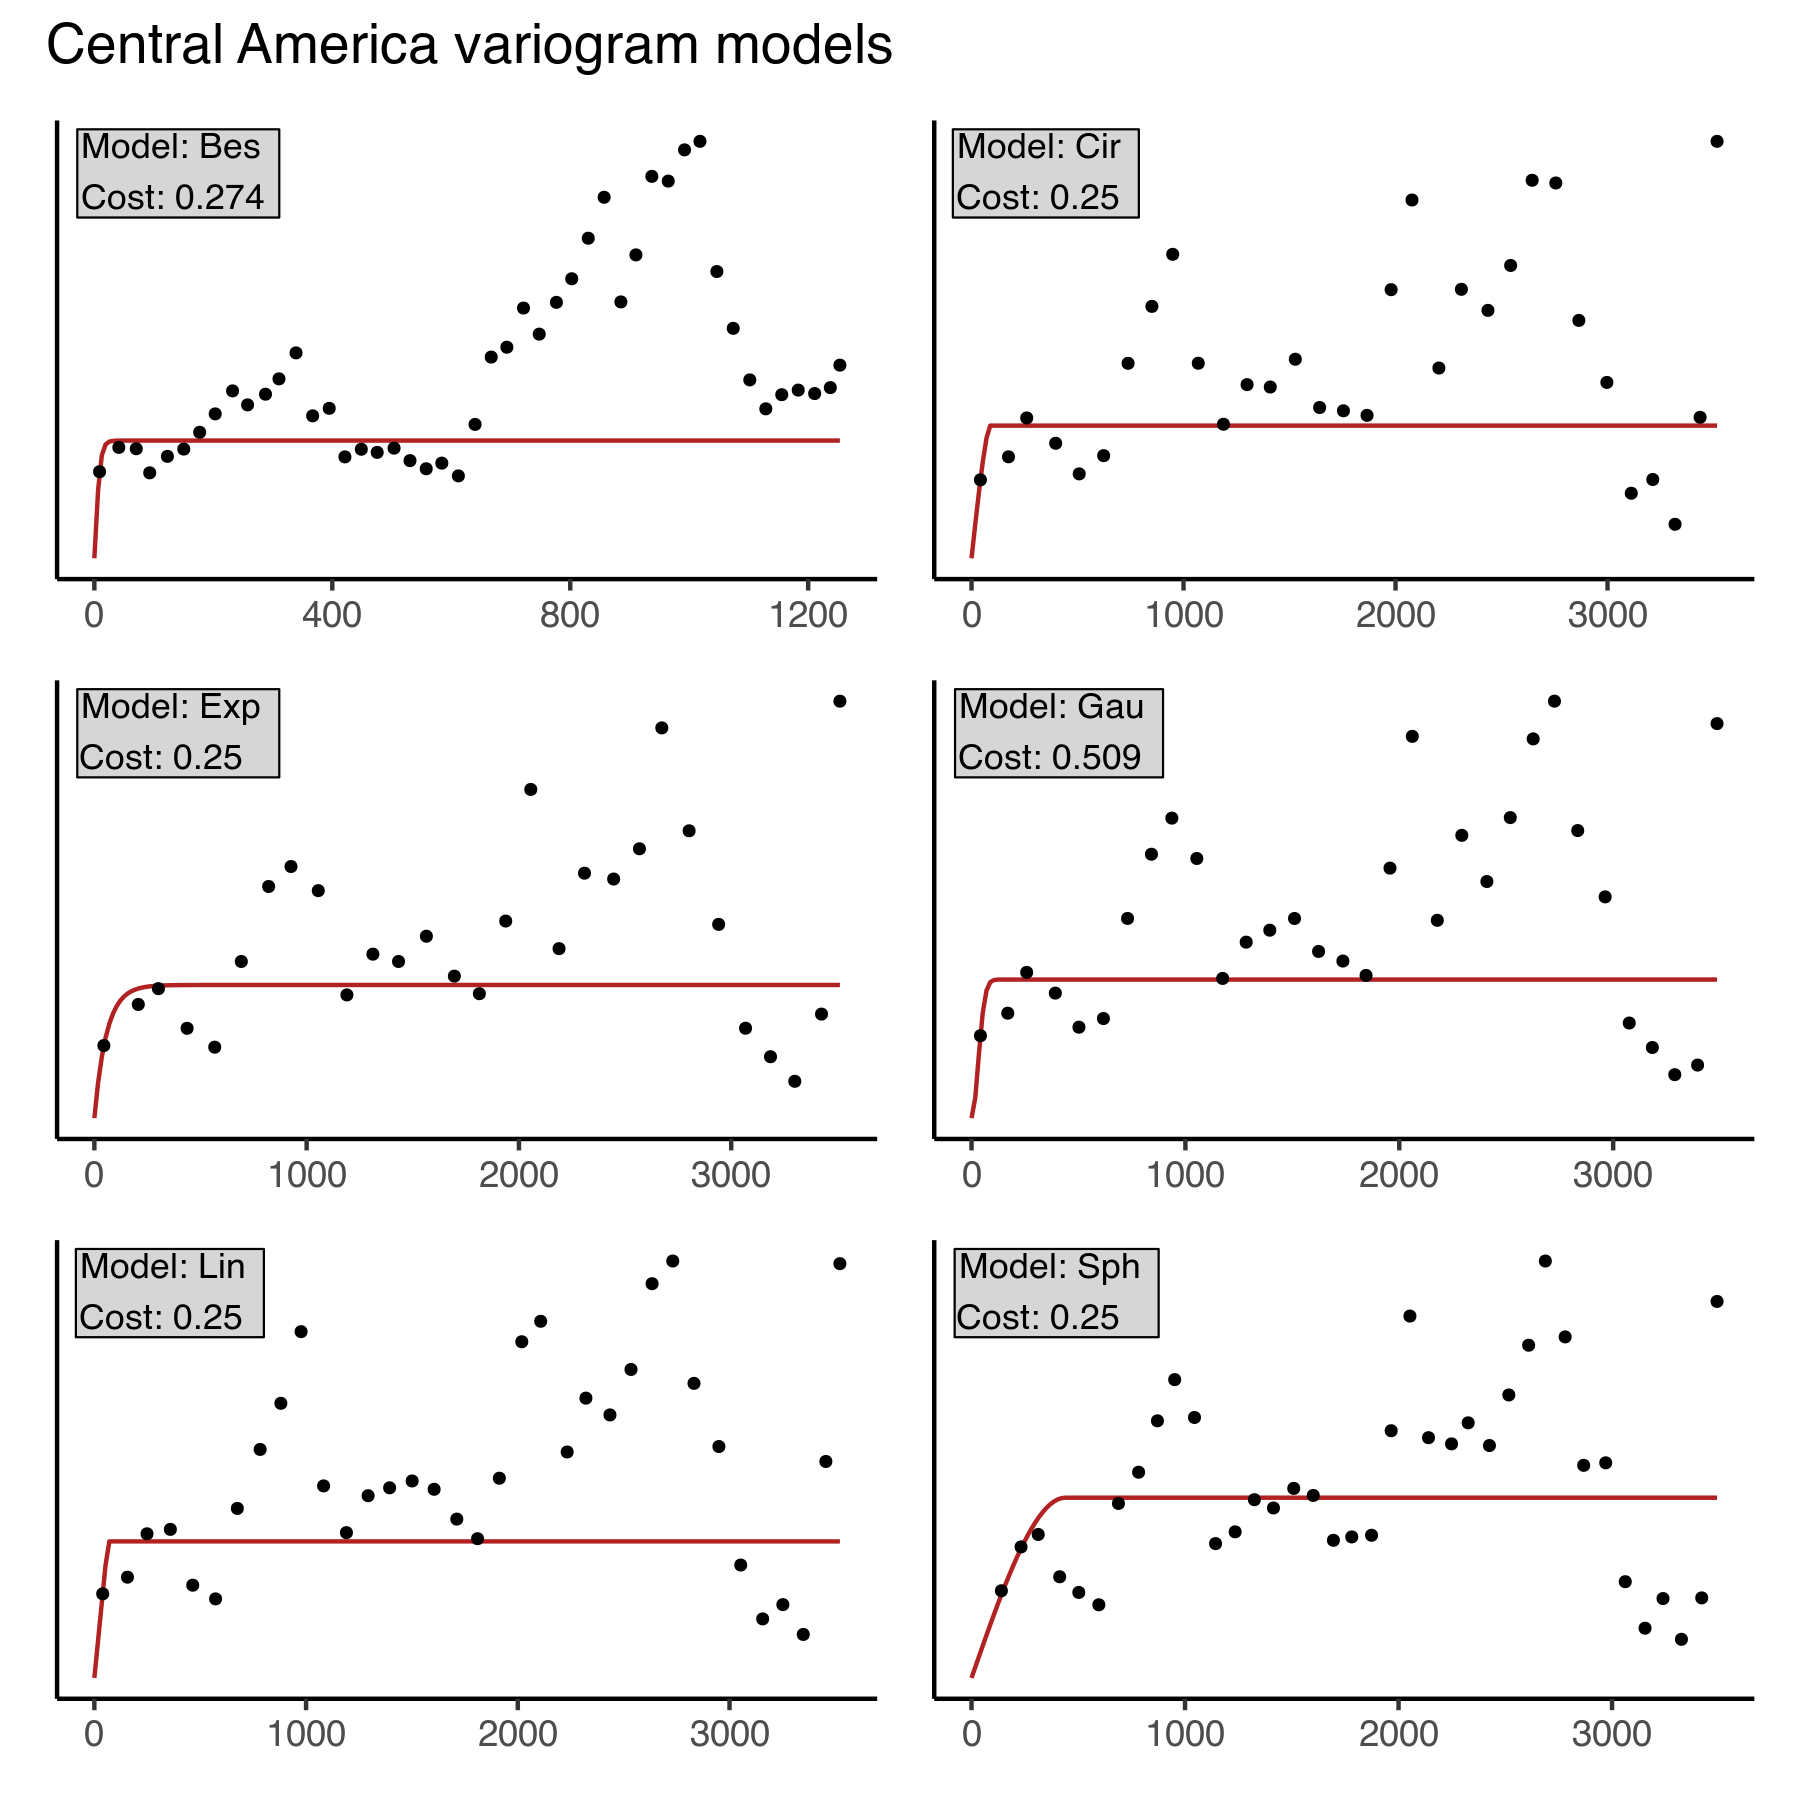
\includegraphics{assets/figs/chpt3/CentralAmericaVgrms.png}
\caption[Fitted variograms for Central America]{Fitted variograms for Central America}
\end{figure}

\begin{figure}
\centering
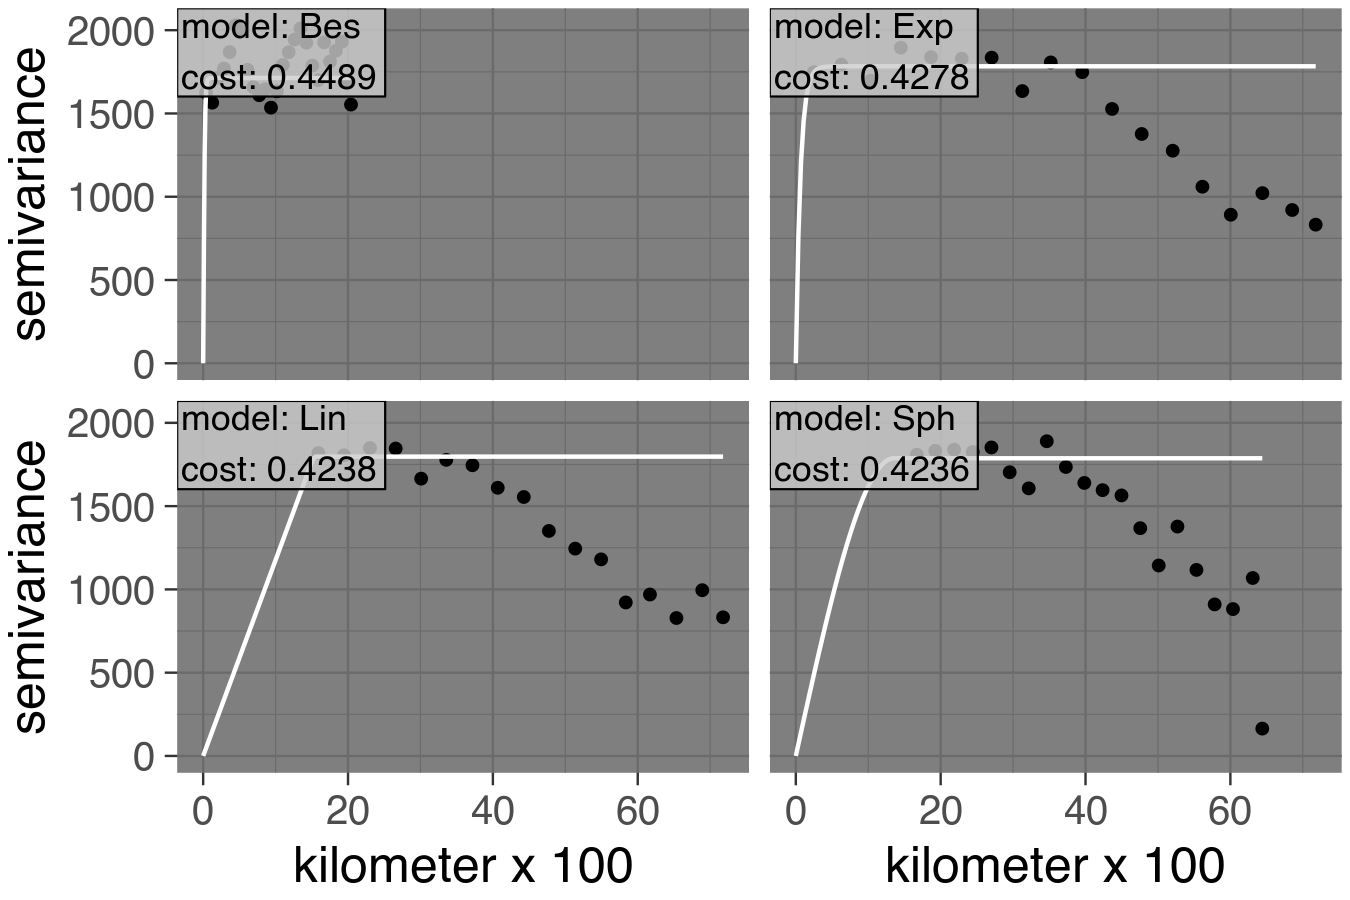
\includegraphics{assets/figs/chpt3/KamchatkaMarianasVgrms.png}
\caption[Fitted variograms for Kamchatka Marianas]{Fitted variograms for Kamchatka Marianas}
\end{figure}

\begin{figure}
\centering
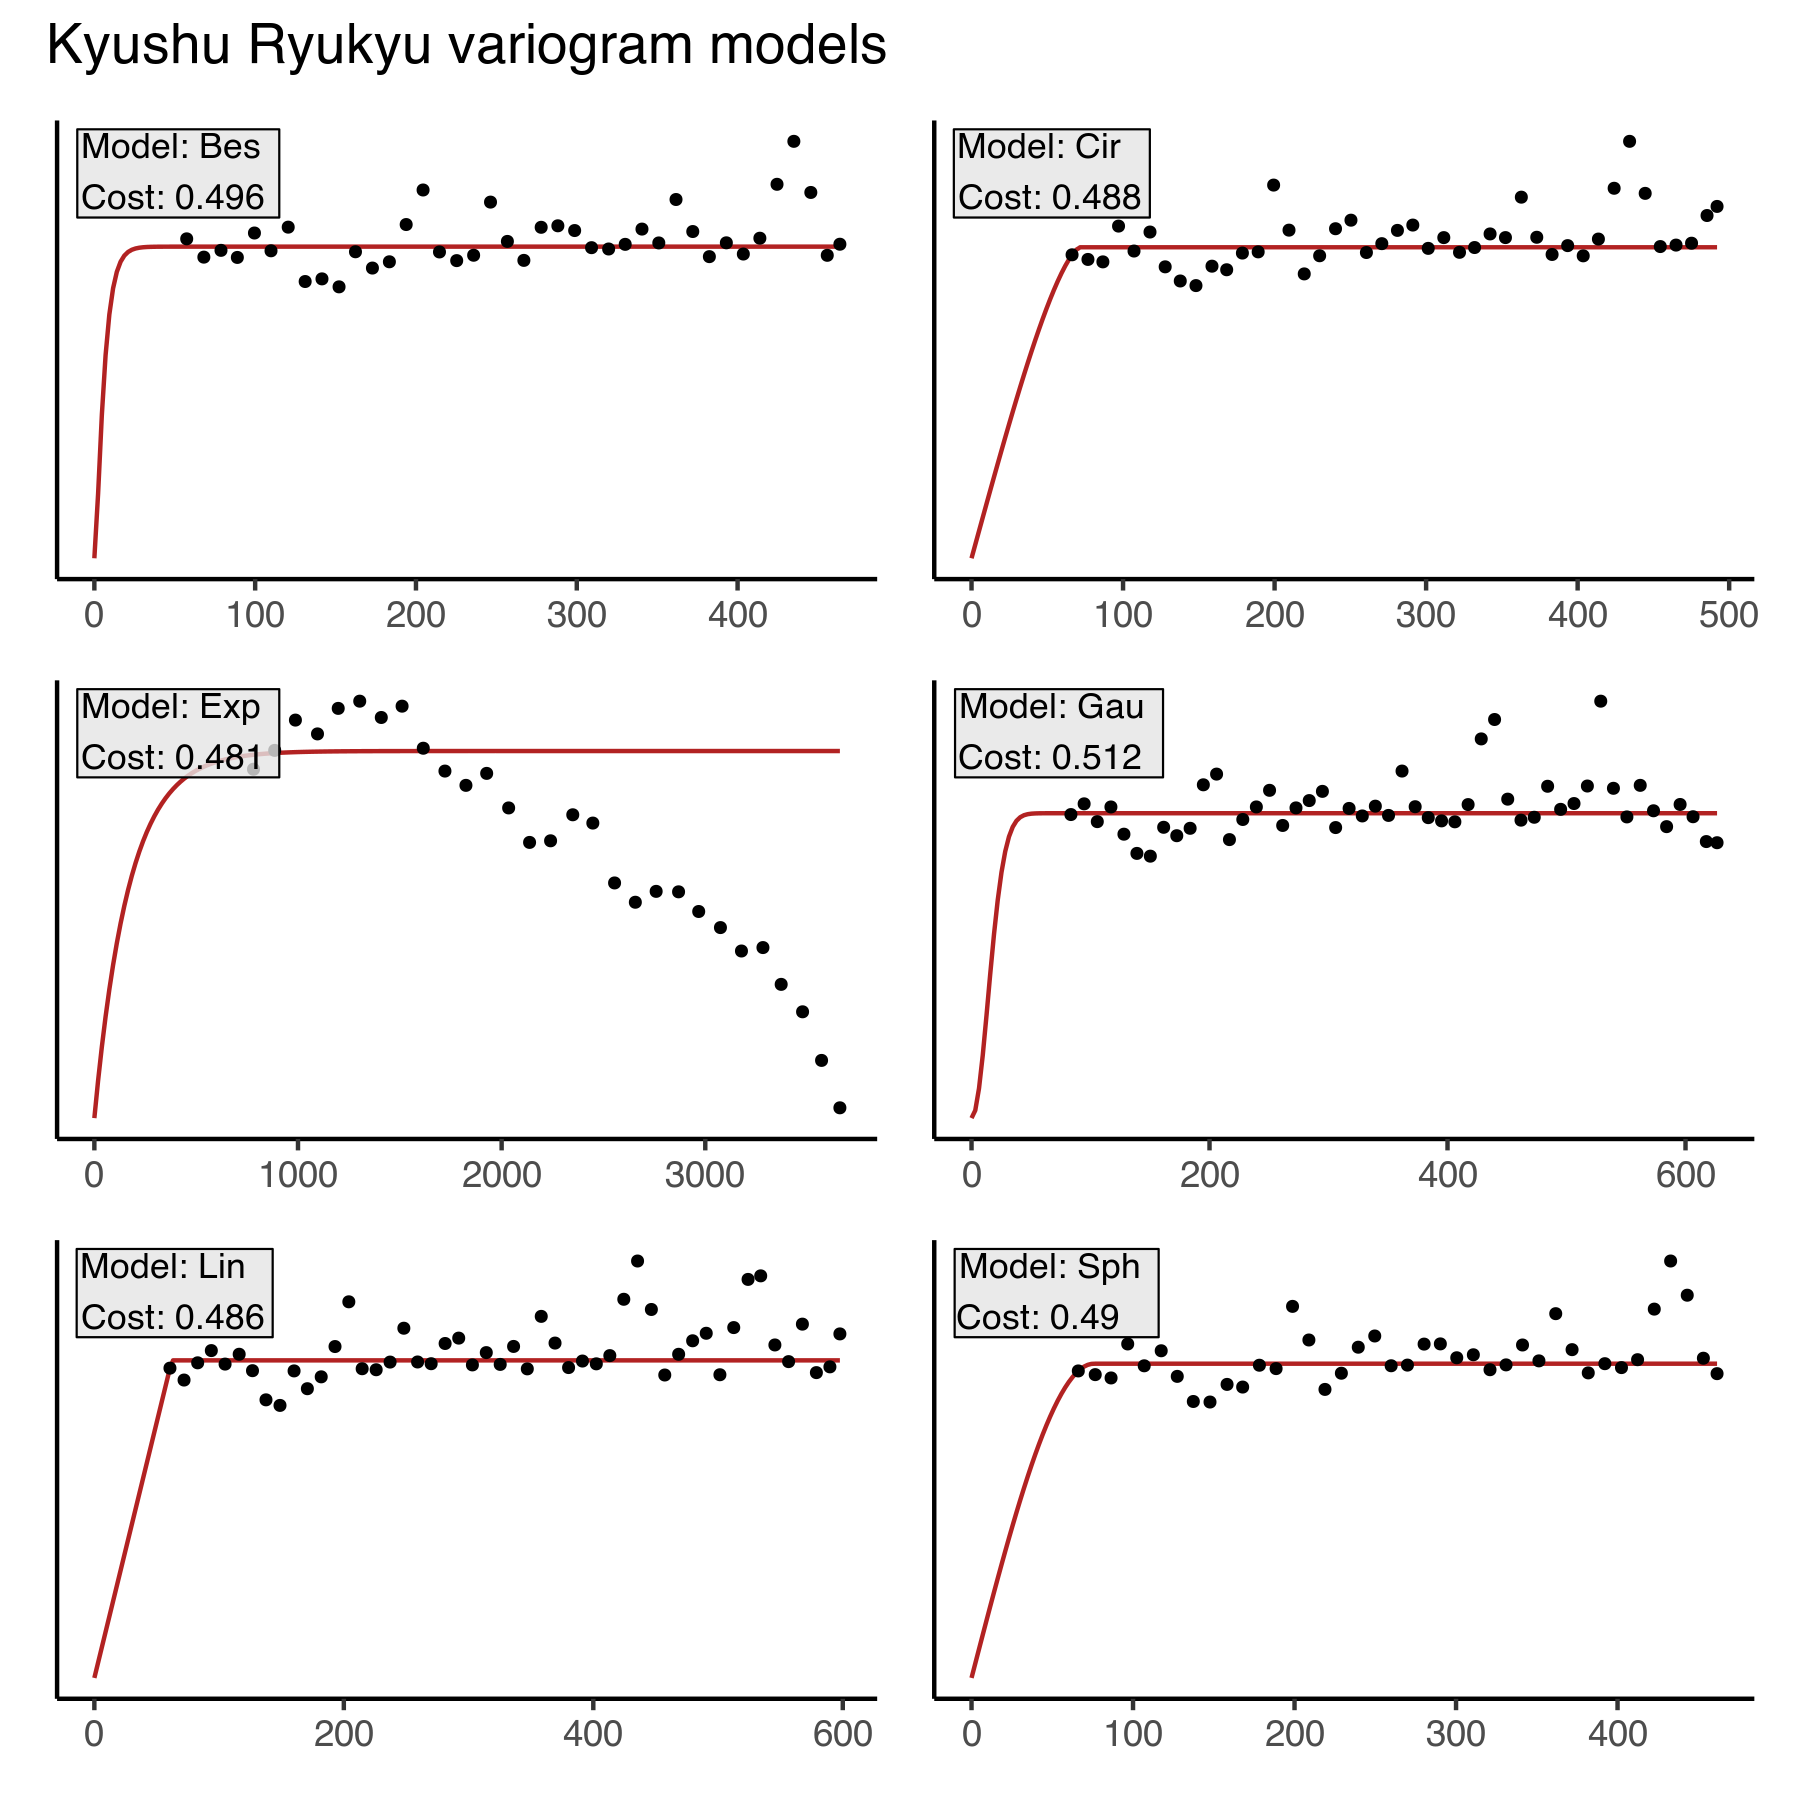
\includegraphics{assets/figs/chpt3/KyushuRyukyuVgrms.png}
\caption[Fitted variograms for Kyushu Ryukyu]{Fitted variograms for Kyushu Ryukyu}
\end{figure}

\begin{figure}
\centering
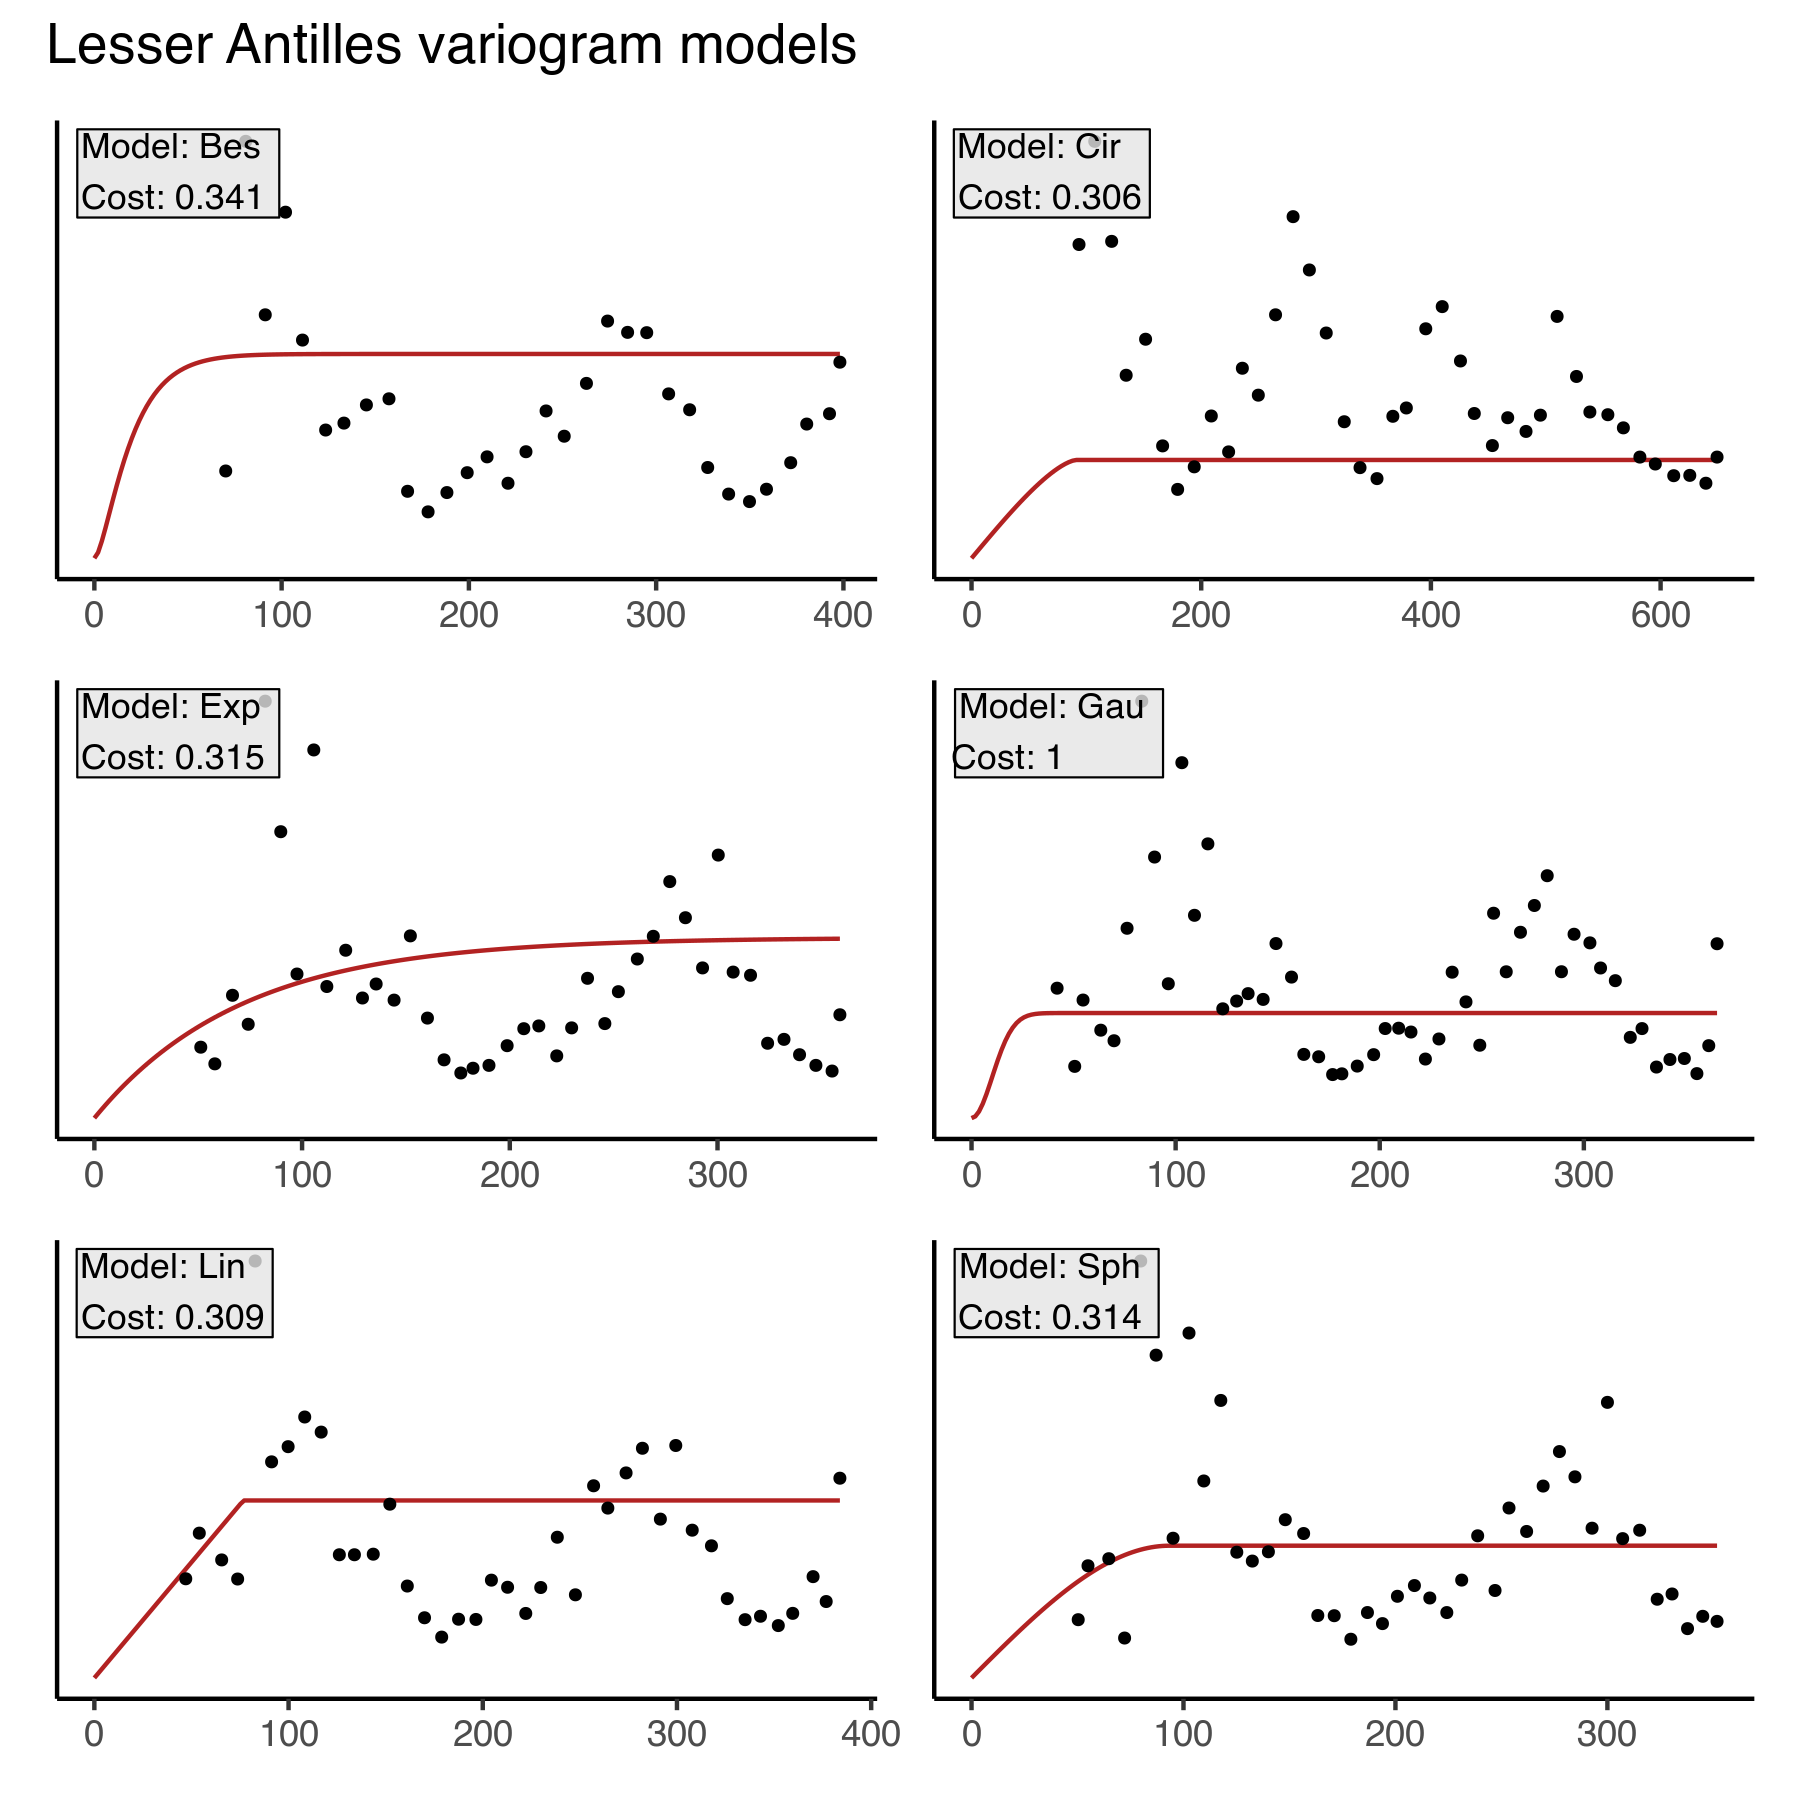
\includegraphics{assets/figs/chpt3/LesserAntillesVgrms.png}
\caption[Fitted variograms for Lesser Antilles]{Fitted variograms for Lesser Antilles}
\end{figure}

\begin{figure}
\centering
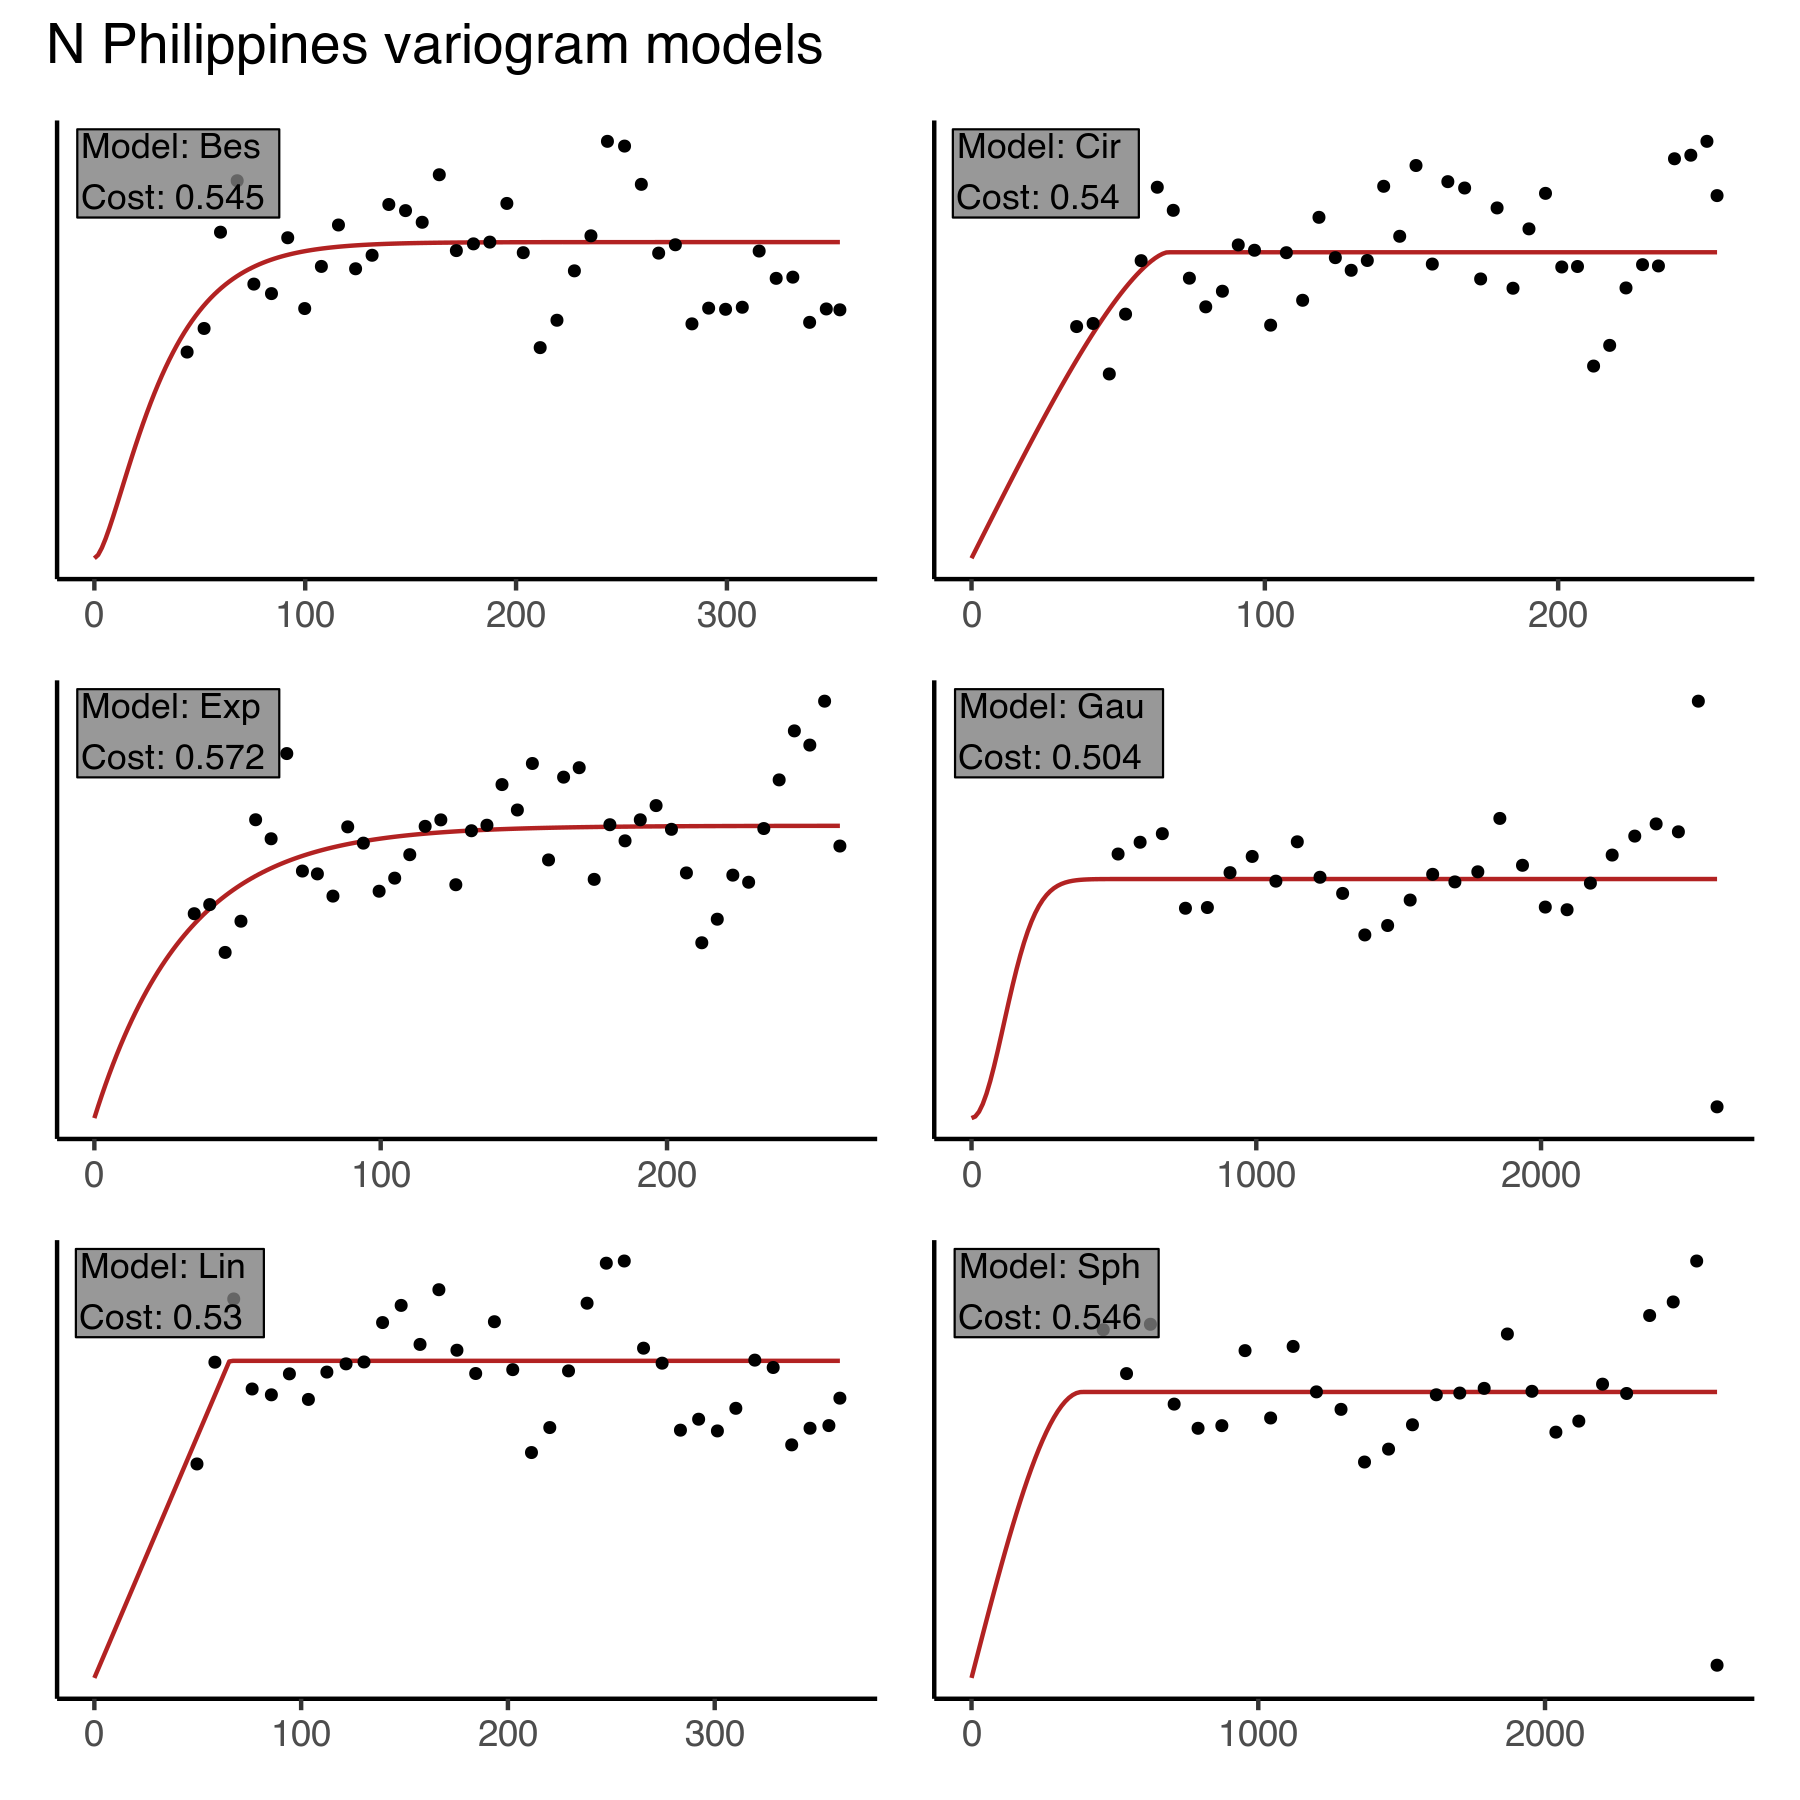
\includegraphics{assets/figs/chpt3/NPhilippinesVgrms.png}
\caption[Fitted variograms for N Philippines]{Fitted variograms for N Philippines}
\end{figure}

\begin{figure}
\centering
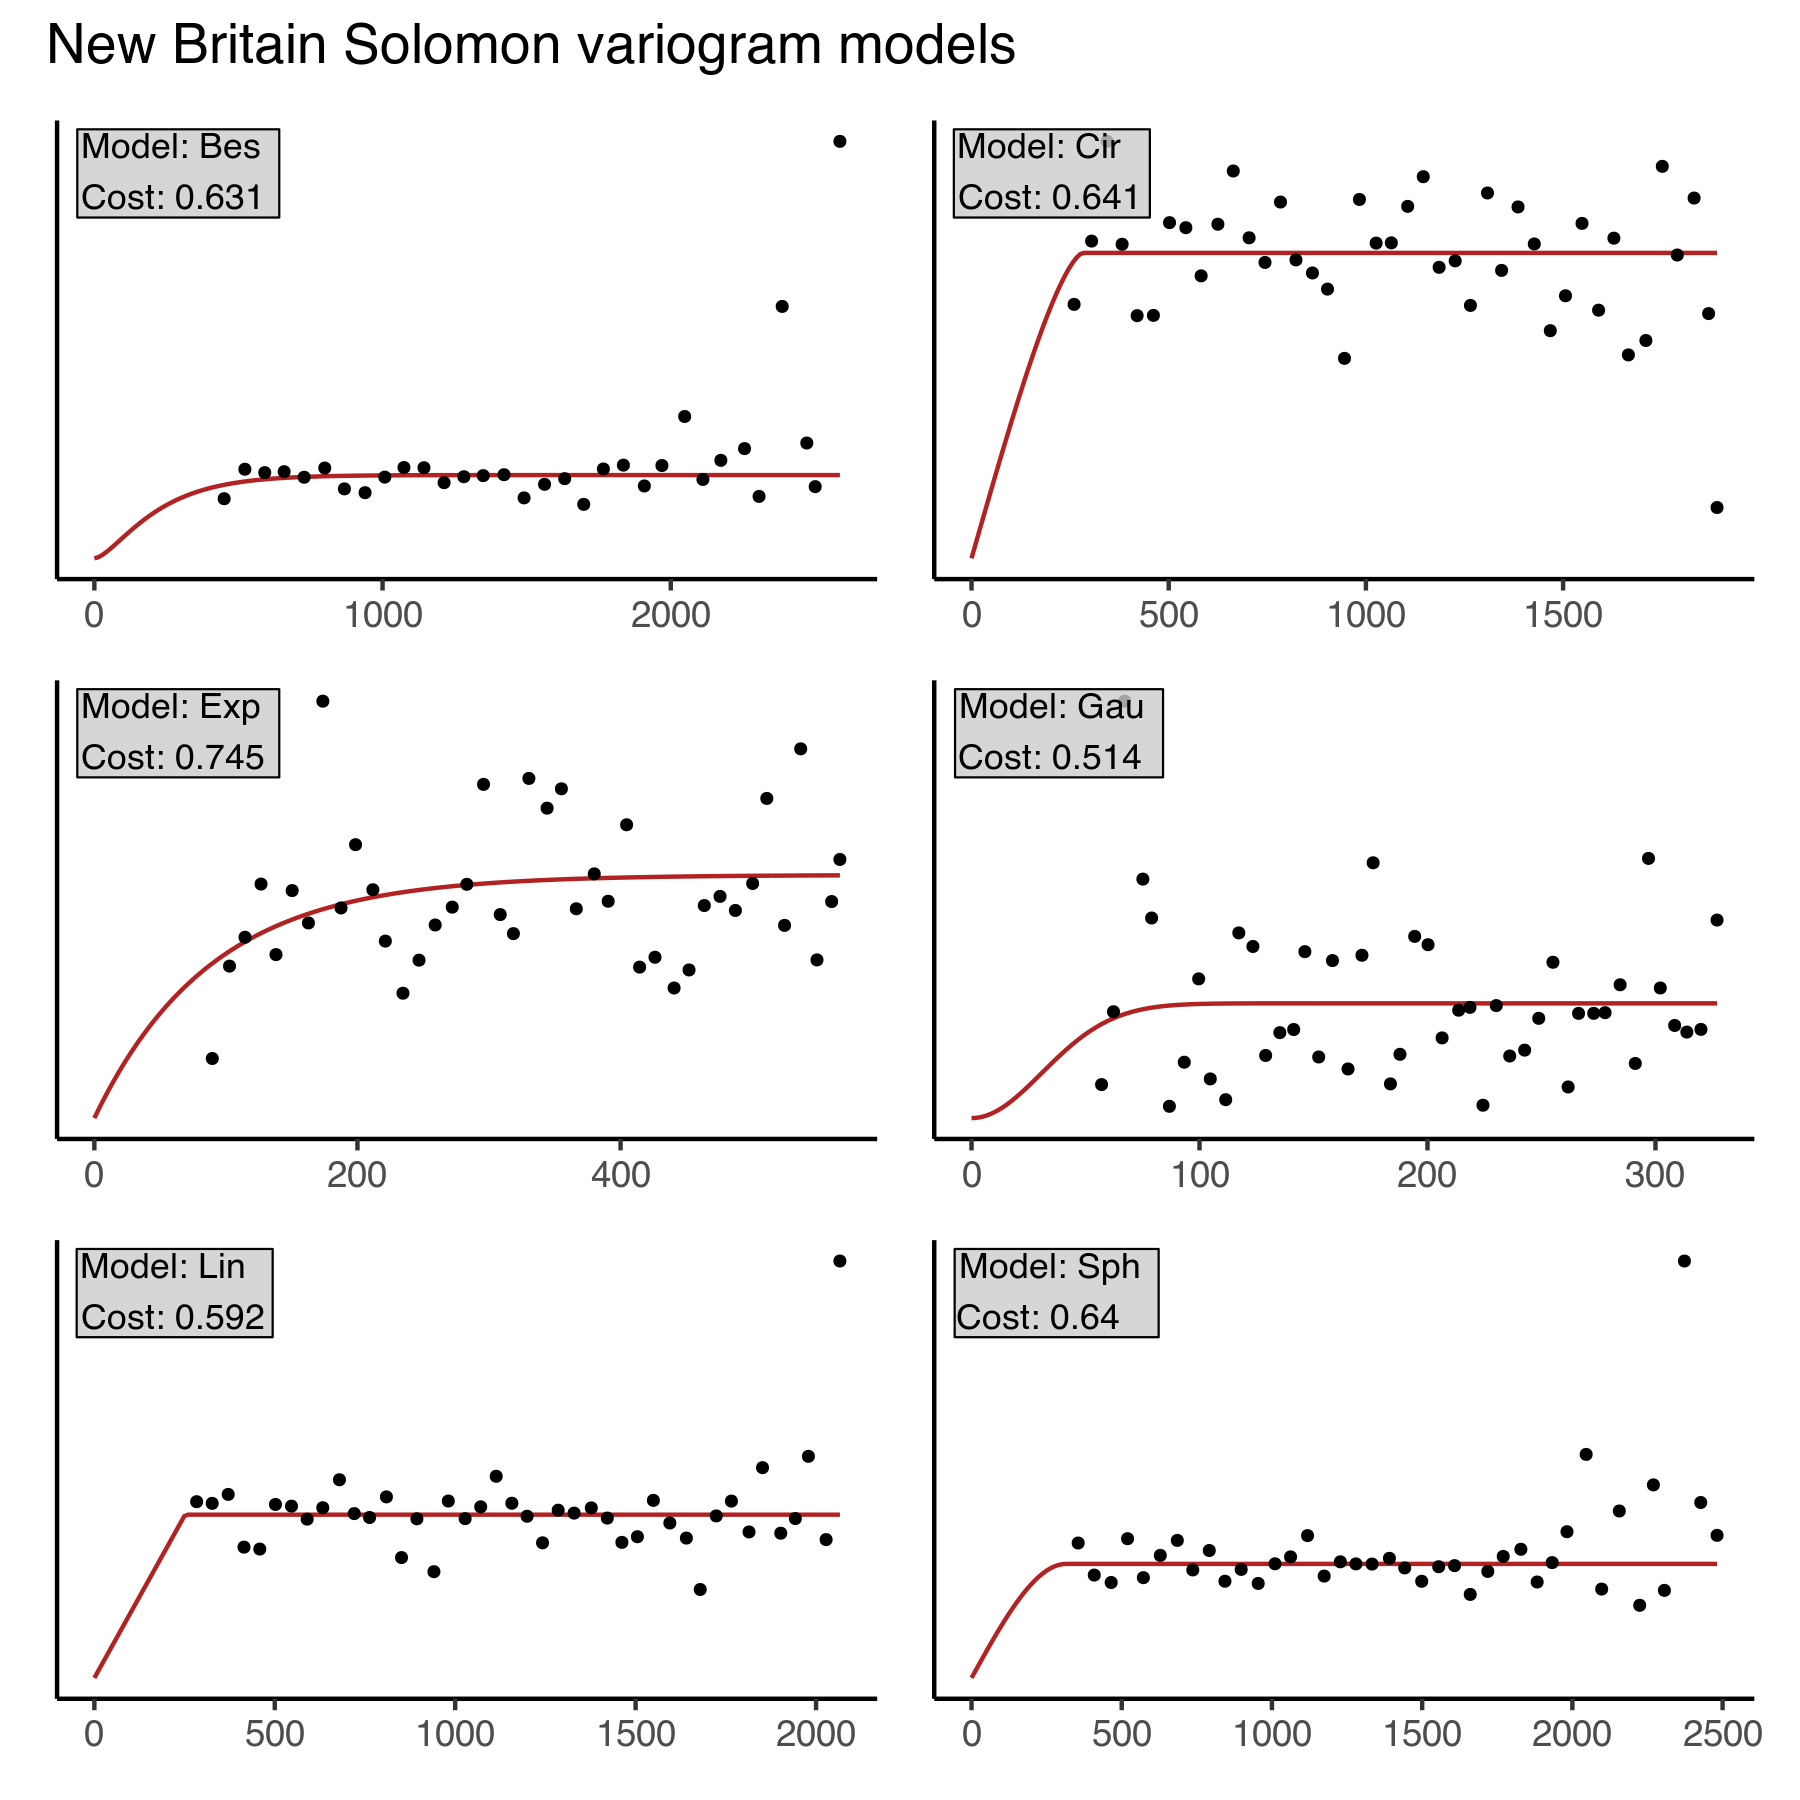
\includegraphics{assets/figs/chpt3/NewBritainSolomonVgrms.png}
\caption[Fitted variograms for New Britain Solomon]{Fitted variograms for New Britain Solomon}
\end{figure}

\begin{figure}
\centering
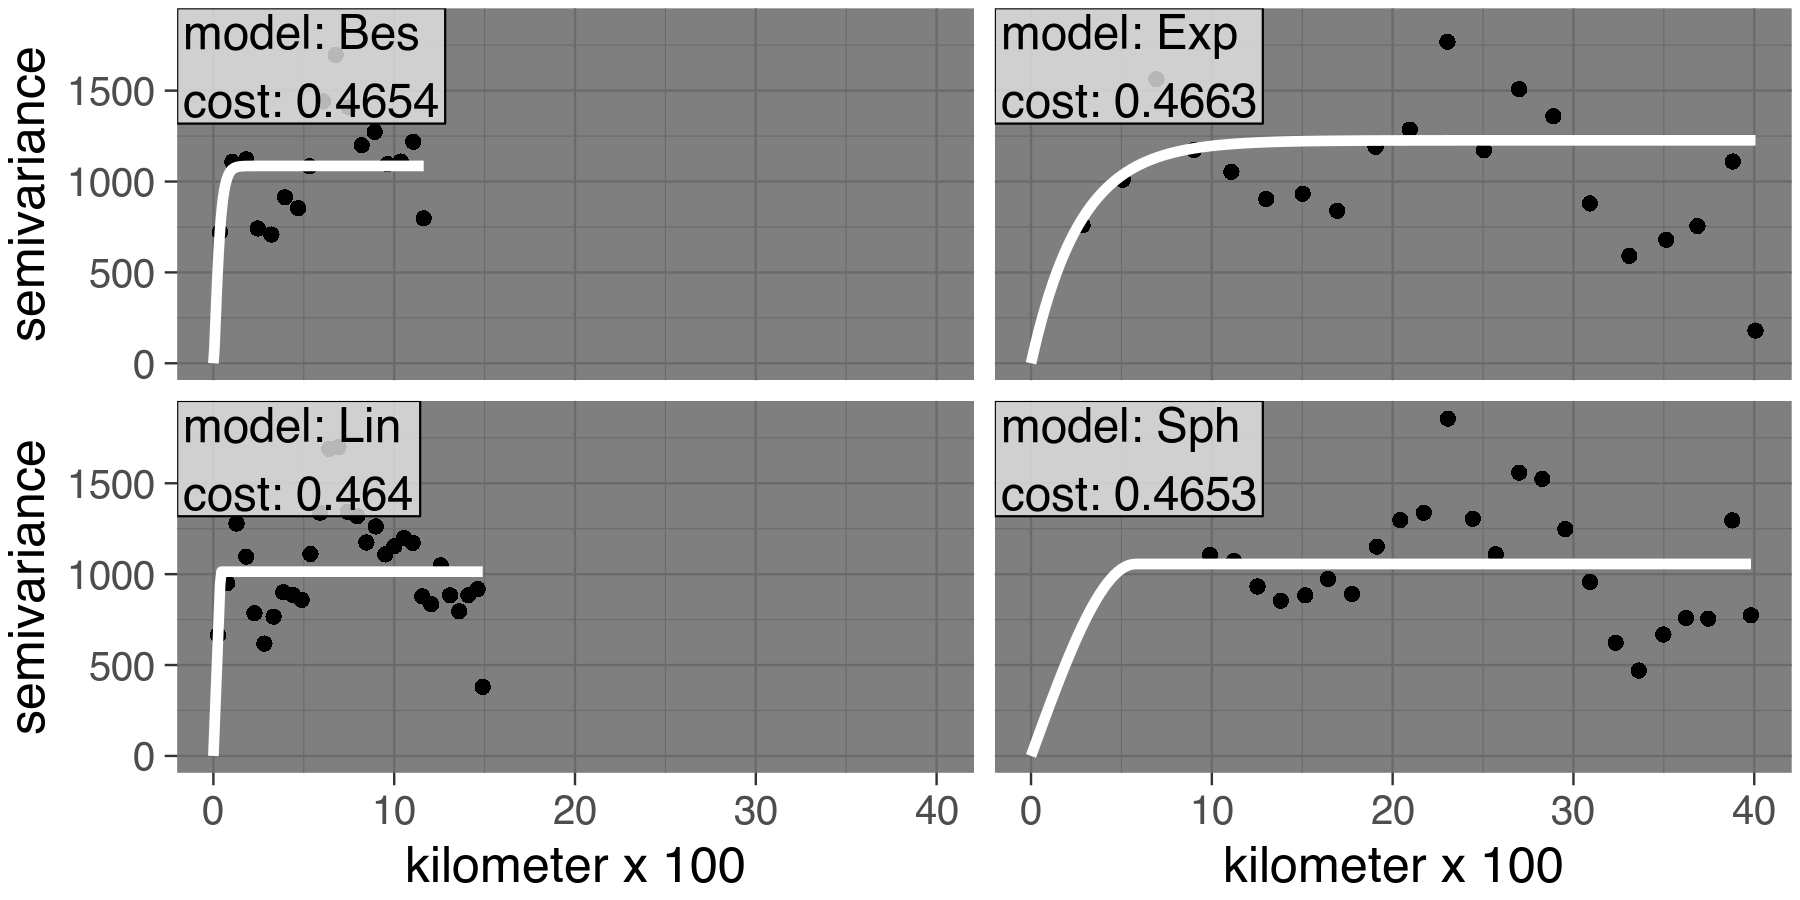
\includegraphics{assets/figs/chpt3/SPhilippinesVgrms.png}
\caption[Fitted variograms for S Philippines]{Fitted variograms for S Philippines}
\end{figure}

\begin{figure}
\centering
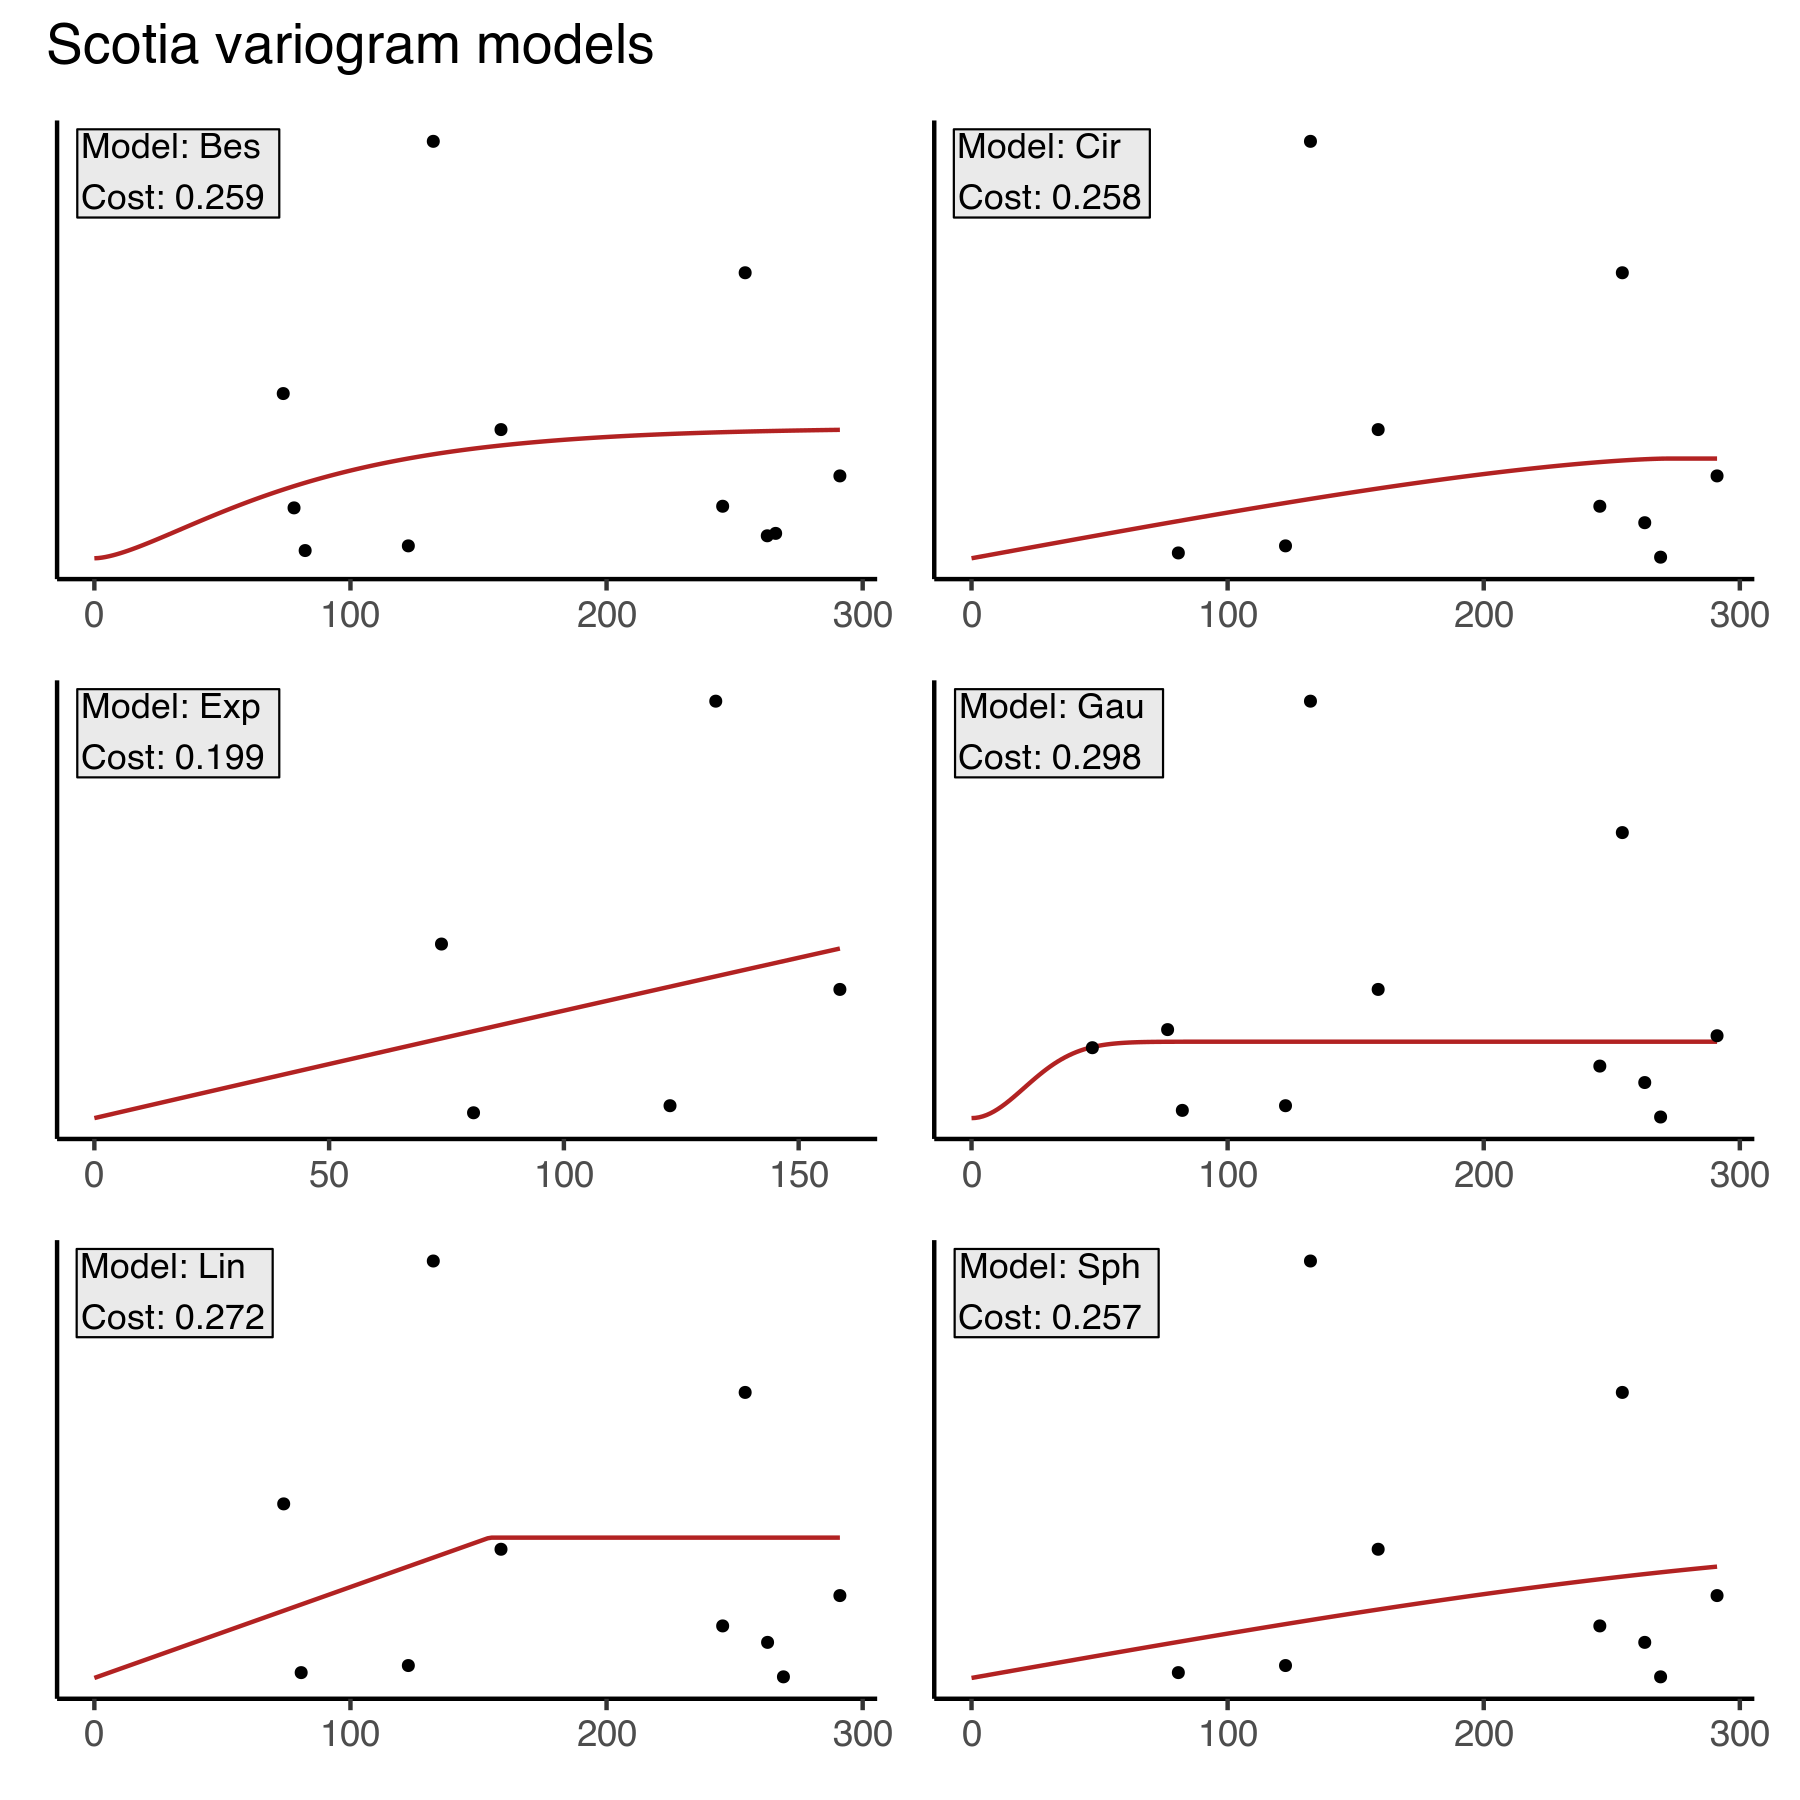
\includegraphics{assets/figs/chpt3/ScotiaVgrms.png}
\caption[Fitted variograms for Scotia]{Fitted variograms for Scotia}
\end{figure}

\begin{figure}
\centering
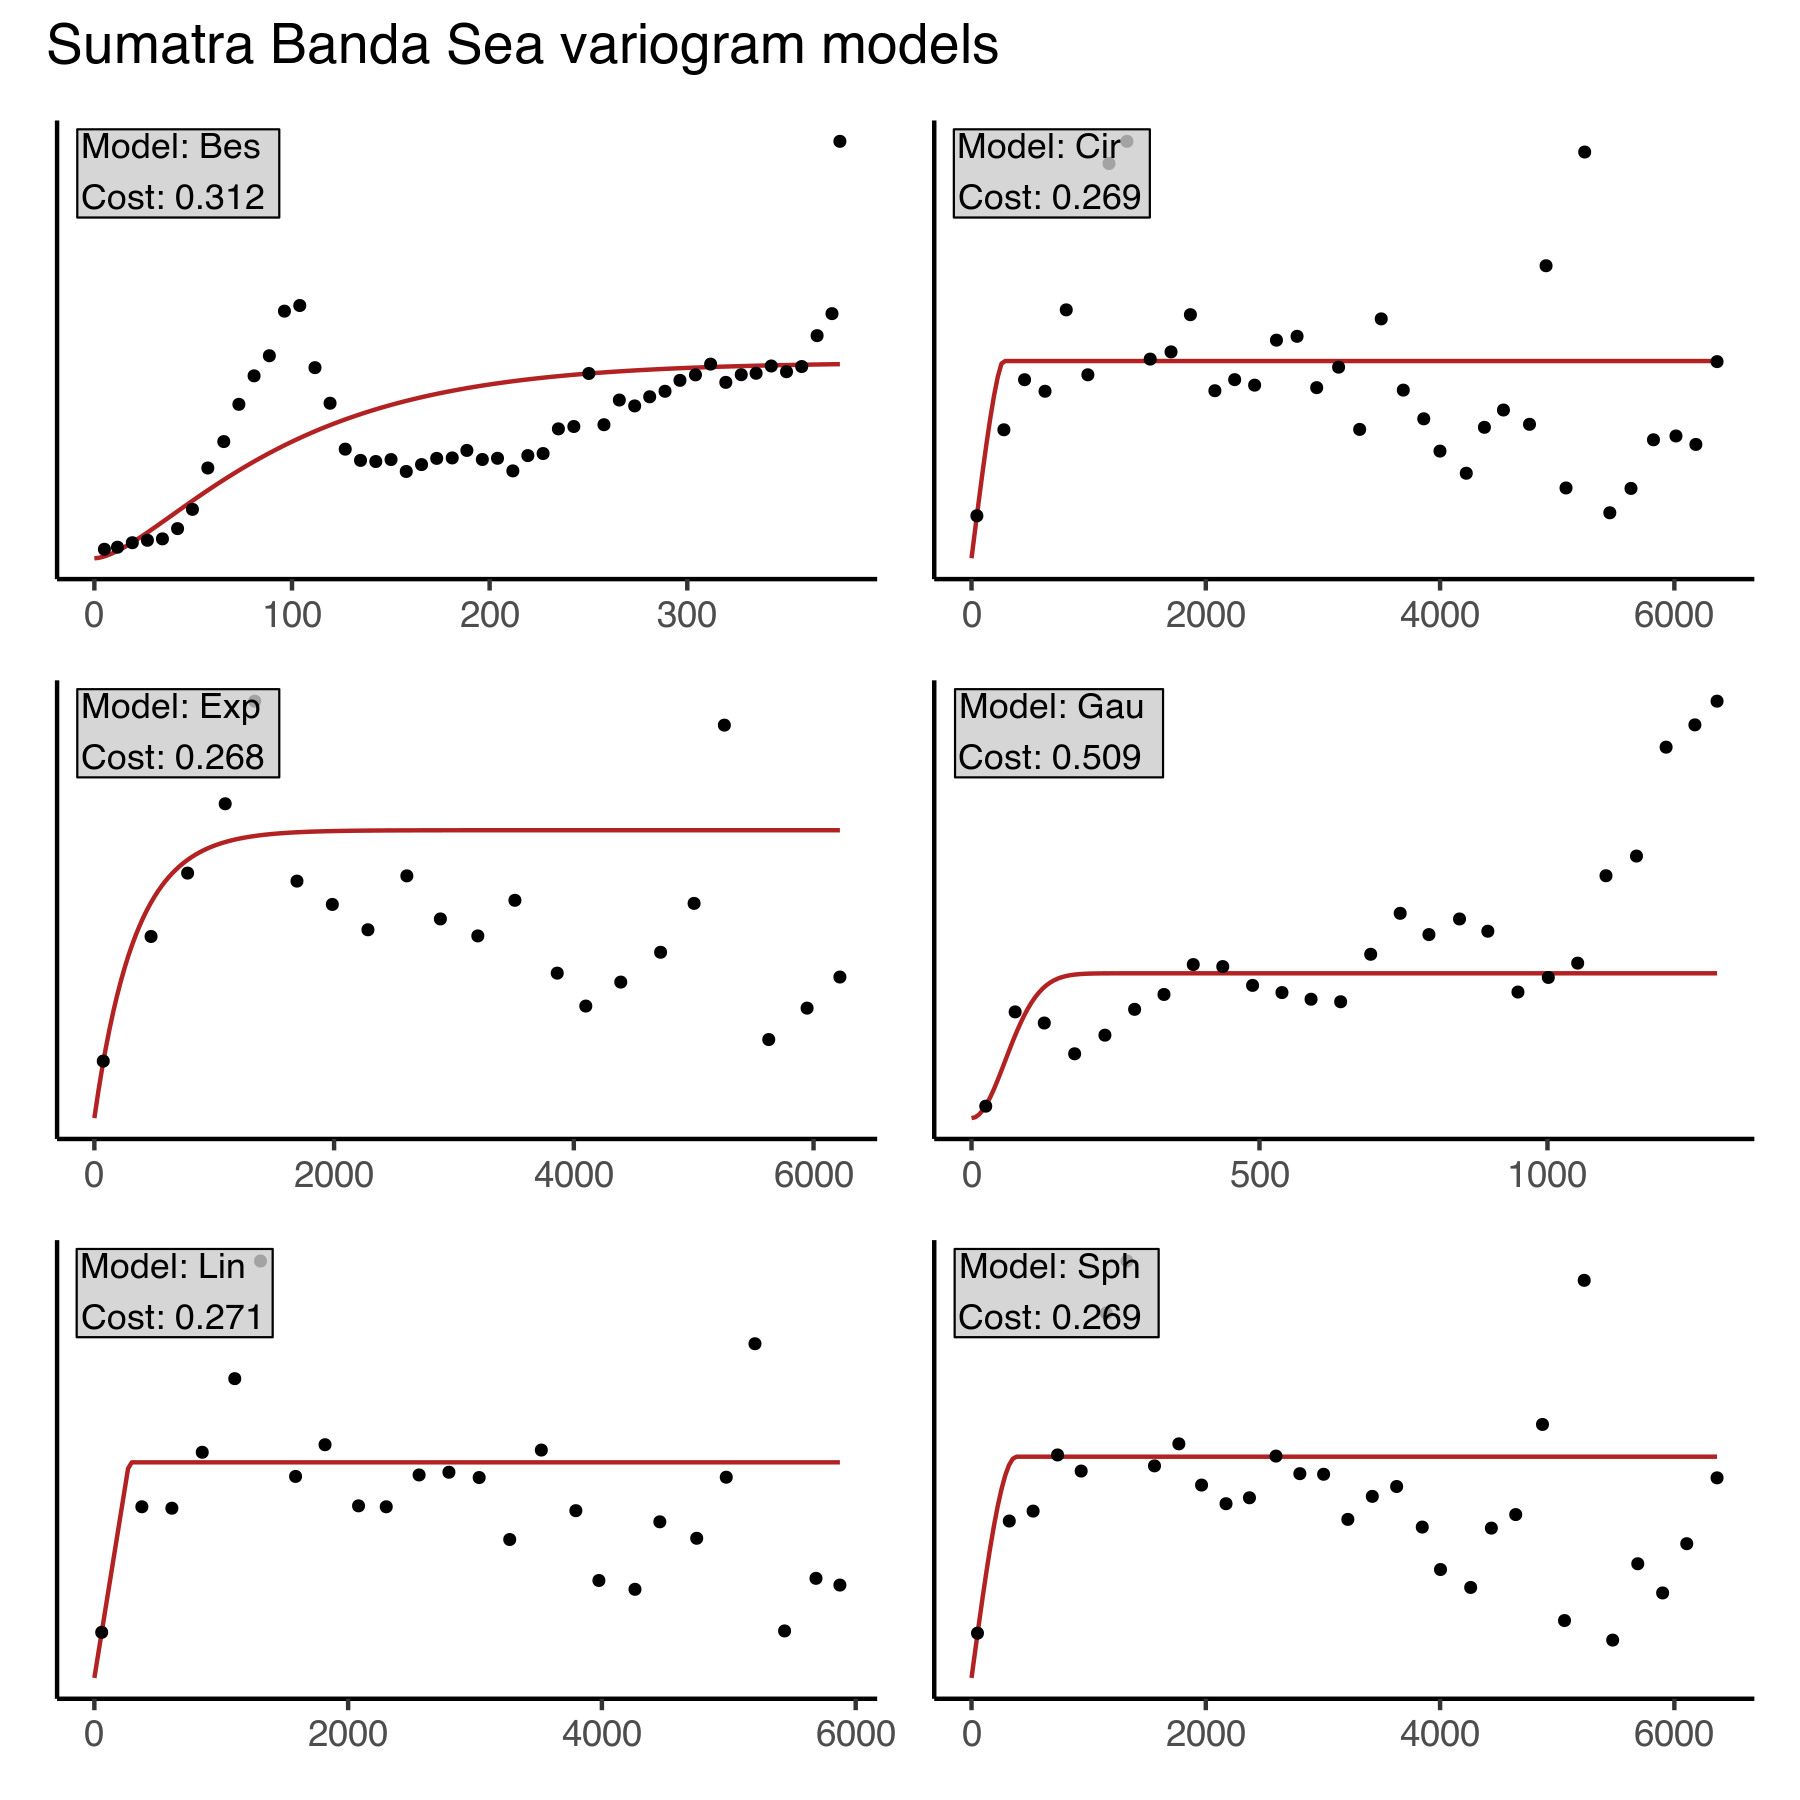
\includegraphics{assets/figs/chpt3/SumatraBandaSeaVgrms.png}
\caption[Fitted variograms for Sumatra Banda Sea]{Fitted variograms for Sumatra Banda Sea}
\end{figure}

\begin{figure}
\centering
\includegraphics{assets/figs/chpt3/TongaNewZealandVgrms.png}
\caption[Fitted variograms for Tonga New Zealand]{Fitted variograms for Tonga New Zealand}
\end{figure}

\begin{figure}
\centering
\includegraphics{assets/figs/chpt3/VanuatuVgrms.png}
\caption[Fitted variograms for Vanuatu]{Fitted variograms for Vanuatu}
\end{figure}

\DIFaddbegin \clearpage

\begingroup
\renewcommand{\arraystretch}{0.5}

\begingroup\fontsize{9}{11}\selectfont

\begin{ThreePartTable}
\begin{TableNotes}
\item \uline{\textit{key}}\DIFadd{: $n_{max}$: max point-pairs, Sill $[(mWm^{-2})^2]$, Range $[km]$, Cost $[mWm^{-2}]$, $RMSE_K$: Kriging accuracy $[mWm^{-2}]$
}\end{TableNotes}
\begin{longtable}[t]{llrrrrrrrr}
\caption{\label{tab:vgrmSummaryTableLong}\DIFadd{Optimum variogram models by segment}}\\
\toprule
\DIFadd{Segment }& \DIFadd{Model }& \DIFadd{Cutoff }& \DIFadd{Lags }& \DIFadd{Shift }& \DIFadd{$n_{max}$ }& \DIFadd{Sill }& \DIFadd{Range }& \DIFadd{Cost }& \DIFadd{$RMSE_K$}\\
\midrule
\endfirsthead
\caption[]{\label{tab:vgrmSummaryTableLong}\DIFadd{Optimum variogram models by segment }\textit{\DIFadd{(continued)}}}\\
\toprule
\DIFadd{Segment }& \DIFadd{Model }& \DIFadd{Cutoff }& \DIFadd{Lags }& \DIFadd{Shift }& \DIFadd{$n_{max}$ }& \DIFadd{Sill }& \DIFadd{Range }& \DIFadd{Cost }& \DIFadd{$RMSE_K$}\\
\midrule
\endhead

\endfoot
\bottomrule
\insertTableNotes
\endlastfoot
\cellcolor{gray!6}{Alaska Aleutians} & \cellcolor{gray!6}{Bes} & \cellcolor{gray!6}{10.4} & \cellcolor{gray!6}{20.8} & \cellcolor{gray!6}{1.5} & \cellcolor{gray!6}{10.9} & \cellcolor{gray!6}{651} & \cellcolor{gray!6}{7} & \cellcolor{gray!6}{0.832} & \cellcolor{gray!6}{26.1}\\
\DIFadd{Alaska Aleutians }& \DIFadd{Cir }& \DIFadd{1.0 }& \DIFadd{15.0 }& \DIFadd{1.6 }& \DIFadd{10.0 }& \DIFadd{824 }& \DIFadd{293 }& \DIFadd{0.662 }& \DIFadd{26.8}\\
\cellcolor{gray!6}{Alaska Aleutians} & \cellcolor{gray!6}{Exp} & \cellcolor{gray!6}{11.4} & \cellcolor{gray!6}{20.9} & \cellcolor{gray!6}{1.6} & \cellcolor{gray!6}{10.2} & \cellcolor{gray!6}{624} & \cellcolor{gray!6}{9} & \cellcolor{gray!6}{0.874} & \cellcolor{gray!6}{25.9}\\
\DIFadd{Alaska Aleutians }& \DIFadd{Gau }& \DIFadd{6.3 }& \DIFadd{23.5 }& \DIFadd{1.6 }& \DIFadd{30.7 }& \DIFadd{707 }& \DIFadd{22 }& \DIFadd{0.508 }& \DIFadd{325.0}\\
\cellcolor{gray!6}{Alaska Aleutians} & \cellcolor{gray!6}{Lin} & \cellcolor{gray!6}{1.0} & \cellcolor{gray!6}{15.0} & \cellcolor{gray!6}{1.6} & \cellcolor{gray!6}{10.0} & \cellcolor{gray!6}{824} & \cellcolor{gray!6}{258} & \cellcolor{gray!6}{0.647} & \cellcolor{gray!6}{26.7}\\
\DIFadd{Alaska Aleutians }& \DIFadd{Sph }& \DIFadd{7.2 }& \DIFadd{15.5 }& \DIFadd{1.6 }& \DIFadd{10.1 }& \DIFadd{750 }& \DIFadd{62 }& \DIFadd{0.781 }& \DIFadd{25.9}\\
\cellcolor{gray!6}{Andes} & \cellcolor{gray!6}{Bes} & \cellcolor{gray!6}{13.5} & \cellcolor{gray!6}{24.0} & \cellcolor{gray!6}{1.5} & \cellcolor{gray!6}{12.0} & \cellcolor{gray!6}{2457} & \cellcolor{gray!6}{5} & \cellcolor{gray!6}{0.319} & \cellcolor{gray!6}{37.4}\\
\DIFadd{Andes }& \DIFadd{Cir }& \DIFadd{10.1 }& \DIFadd{20.5 }& \DIFadd{1.6 }& \DIFadd{11.8 }& \DIFadd{2476 }& \DIFadd{20 }& \DIFadd{0.308 }& \DIFadd{35.1}\\
\cellcolor{gray!6}{Andes} & \cellcolor{gray!6}{Exp} & \cellcolor{gray!6}{7.3} & \cellcolor{gray!6}{24.8} & \cellcolor{gray!6}{1.6} & \cellcolor{gray!6}{11.9} & \cellcolor{gray!6}{2575} & \cellcolor{gray!6}{12} & \cellcolor{gray!6}{0.306} & \cellcolor{gray!6}{34.8}\\
\DIFadd{Andes }& \DIFadd{Gau }& \DIFadd{3.5 }& \DIFadd{18.4 }& \DIFadd{1.6 }& \DIFadd{29.4 }& \DIFadd{3327 }& \DIFadd{49 }& \DIFadd{0.511 }& \DIFadd{339864515.0}\\
\cellcolor{gray!6}{Andes} & \cellcolor{gray!6}{Lin} & \cellcolor{gray!6}{9.0} & \cellcolor{gray!6}{25.5} & \cellcolor{gray!6}{1.5} & \cellcolor{gray!6}{19.6} & \cellcolor{gray!6}{2565} & \cellcolor{gray!6}{17} & \cellcolor{gray!6}{0.315} & \cellcolor{gray!6}{35.7}\\
\DIFadd{Andes }& \DIFadd{Sph }& \DIFadd{9.7 }& \DIFadd{22.5 }& \DIFadd{1.6 }& \DIFadd{11.7 }& \DIFadd{2499 }& \DIFadd{23 }& \DIFadd{0.307 }& \DIFadd{35.1}\\
\cellcolor{gray!6}{Central America} & \cellcolor{gray!6}{Bes} & \cellcolor{gray!6}{12.2} & \cellcolor{gray!6}{23.6} & \cellcolor{gray!6}{1.5} & \cellcolor{gray!6}{17.1} & \cellcolor{gray!6}{1985} & \cellcolor{gray!6}{3} & \cellcolor{gray!6}{0.280} & \cellcolor{gray!6}{33.3}\\
\DIFadd{Central America }& \DIFadd{Cir }& \DIFadd{13.0 }& \DIFadd{24.7 }& \DIFadd{1.3 }& \DIFadd{11.2 }& \DIFadd{2038 }& \DIFadd{10 }& \DIFadd{0.262 }& \DIFadd{30.9}\\
\cellcolor{gray!6}{Central America} & \cellcolor{gray!6}{Exp} & \cellcolor{gray!6}{12.5} & \cellcolor{gray!6}{27.1} & \cellcolor{gray!6}{1.5} & \cellcolor{gray!6}{11.8} & \cellcolor{gray!6}{2076} & \cellcolor{gray!6}{5} & \cellcolor{gray!6}{0.266} & \cellcolor{gray!6}{30.7}\\
\DIFadd{Central America }& \DIFadd{Gau }& \DIFadd{12.6 }& \DIFadd{23.7 }& \DIFadd{2.0 }& \DIFadd{30.2 }& \DIFadd{1998 }& \DIFadd{5 }& \DIFadd{0.536 }& \DIFadd{1514264.0}\\
\cellcolor{gray!6}{Central America} & \cellcolor{gray!6}{Lin} & \cellcolor{gray!6}{12.9} & \cellcolor{gray!6}{25.9} & \cellcolor{gray!6}{1.6} & \cellcolor{gray!6}{17.0} & \cellcolor{gray!6}{2048} & \cellcolor{gray!6}{8} & \cellcolor{gray!6}{0.267} & \cellcolor{gray!6}{31.0}\\
\DIFadd{Central America }& \DIFadd{Sph }& \DIFadd{12.8 }& \DIFadd{37.5 }& \DIFadd{1.5 }& \DIFadd{12.1 }& \DIFadd{2212 }& \DIFadd{12 }& \DIFadd{0.267 }& \DIFadd{31.0}\\
\cellcolor{gray!6}{Kamchatka Marianas} & \cellcolor{gray!6}{Bes} & \cellcolor{gray!6}{11.5} & \cellcolor{gray!6}{22.7} & \cellcolor{gray!6}{1.6} & \cellcolor{gray!6}{12.2} & \cellcolor{gray!6}{1725} & \cellcolor{gray!6}{5} & \cellcolor{gray!6}{0.458} & \cellcolor{gray!6}{32.2}\\
\DIFadd{Kamchatka Marianas }& \DIFadd{Cir }& \DIFadd{1.0 }& \DIFadd{20.8 }& \DIFadd{1.6 }& \DIFadd{10.1 }& \DIFadd{1792 }& \DIFadd{251 }& \DIFadd{0.430 }& \DIFadd{32.1}\\
\cellcolor{gray!6}{Kamchatka Marianas} & \cellcolor{gray!6}{Exp} & \cellcolor{gray!6}{11.1} & \cellcolor{gray!6}{23.7} & \cellcolor{gray!6}{1.6} & \cellcolor{gray!6}{10.9} & \cellcolor{gray!6}{1726} & \cellcolor{gray!6}{7} & \cellcolor{gray!6}{0.461} & \cellcolor{gray!6}{30.9}\\
\DIFadd{Kamchatka Marianas }& \DIFadd{Gau }& \DIFadd{12.2 }& \DIFadd{16.9 }& \DIFadd{1.6 }& \DIFadd{29.4 }& \DIFadd{1692 }& \DIFadd{10 }& \DIFadd{0.521 }& \DIFadd{3085159.0}\\
\cellcolor{gray!6}{Kamchatka Marianas} & \cellcolor{gray!6}{Lin} & \cellcolor{gray!6}{15.2} & \cellcolor{gray!6}{33.4} & \cellcolor{gray!6}{1.6} & \cellcolor{gray!6}{10.0} & \cellcolor{gray!6}{1796} & \cellcolor{gray!6}{11} & \cellcolor{gray!6}{0.458} & \cellcolor{gray!6}{31.3}\\
\DIFadd{Kamchatka Marianas }& \DIFadd{Sph }& \DIFadd{1.0 }& \DIFadd{17.3 }& \DIFadd{2.1 }& \DIFadd{11.2 }& \DIFadd{1799 }& \DIFadd{814 }& \DIFadd{0.426 }& \DIFadd{32.0}\\
\cellcolor{gray!6}{Kyushu Ryukyu} & \cellcolor{gray!6}{Bes} & \cellcolor{gray!6}{13.4} & \cellcolor{gray!6}{22.9} & \cellcolor{gray!6}{1.5} & \cellcolor{gray!6}{12.6} & \cellcolor{gray!6}{2045} & \cellcolor{gray!6}{4} & \cellcolor{gray!6}{0.509} & \cellcolor{gray!6}{35.1}\\
\DIFadd{Kyushu Ryukyu }& \DIFadd{Cir }& \DIFadd{1.0 }& \DIFadd{27.4 }& \DIFadd{1.0 }& \DIFadd{15.9 }& \DIFadd{1882 }& \DIFadd{73 }& \DIFadd{0.485 }& \DIFadd{35.0}\\
\cellcolor{gray!6}{Kyushu Ryukyu} & \cellcolor{gray!6}{Exp} & \cellcolor{gray!6}{12.9} & \cellcolor{gray!6}{23.3} & \cellcolor{gray!6}{1.8} & \cellcolor{gray!6}{10.9} & \cellcolor{gray!6}{2047} & \cellcolor{gray!6}{6} & \cellcolor{gray!6}{0.513} & \cellcolor{gray!6}{32.5}\\
\DIFadd{Kyushu Ryukyu }& \DIFadd{Gau }& \DIFadd{12.6 }& \DIFadd{23.1 }& \DIFadd{1.1 }& \DIFadd{30.5 }& \DIFadd{2046 }& \DIFadd{6 }& \DIFadd{0.524 }& \DIFadd{1010763.0}\\
\cellcolor{gray!6}{Kyushu Ryukyu} & \cellcolor{gray!6}{Lin} & \cellcolor{gray!6}{1.0} & \cellcolor{gray!6}{20.5} & \cellcolor{gray!6}{1.5} & \cellcolor{gray!6}{31.9} & \cellcolor{gray!6}{1873} & \cellcolor{gray!6}{119} & \cellcolor{gray!6}{0.484} & \cellcolor{gray!6}{35.8}\\
\DIFadd{Kyushu Ryukyu }& \DIFadd{Sph }& \DIFadd{7.0 }& \DIFadd{20.8 }& \DIFadd{1.6 }& \DIFadd{12.8 }& \DIFadd{1888 }& \DIFadd{17 }& \DIFadd{0.500 }& \DIFadd{32.6}\\
\cellcolor{gray!6}{Lesser Antilles} & \cellcolor{gray!6}{Bes} & \cellcolor{gray!6}{17.2} & \cellcolor{gray!6}{21.9} & \cellcolor{gray!6}{1.5} & \cellcolor{gray!6}{29.8} & \cellcolor{gray!6}{305} & \cellcolor{gray!6}{13} & \cellcolor{gray!6}{0.356} & \cellcolor{gray!6}{10.5}\\
\DIFadd{Lesser Antilles }& \DIFadd{Cir }& \DIFadd{12.6 }& \DIFadd{29.2 }& \DIFadd{1.6 }& \DIFadd{29.6 }& \DIFadd{916 }& \DIFadd{143 }& \DIFadd{0.321 }& \DIFadd{9.7}\\
\cellcolor{gray!6}{Lesser Antilles} & \cellcolor{gray!6}{Exp} & \cellcolor{gray!6}{11.6} & \cellcolor{gray!6}{19.7} & \cellcolor{gray!6}{1.6} & \cellcolor{gray!6}{29.0} & \cellcolor{gray!6}{3424} & \cellcolor{gray!6}{409} & \cellcolor{gray!6}{0.319} & \cellcolor{gray!6}{9.7}\\
\DIFadd{Lesser Antilles }& \DIFadd{Gau }& \DIFadd{12.7 }& \DIFadd{23.0 }& \DIFadd{1.2 }& \DIFadd{30.5 }& \DIFadd{208 }& \DIFadd{13 }&  & \\
\cellcolor{gray!6}{Lesser Antilles} & \cellcolor{gray!6}{Lin} & \cellcolor{gray!6}{17.3} & \cellcolor{gray!6}{21.6} & \cellcolor{gray!6}{1.6} & \cellcolor{gray!6}{29.2} & \cellcolor{gray!6}{616} & \cellcolor{gray!6}{75} & \cellcolor{gray!6}{0.318} & \cellcolor{gray!6}{9.7}\\
\DIFadd{Lesser Antilles }& \DIFadd{Sph }& \DIFadd{2.9 }& \DIFadd{27.2 }& \DIFadd{1.5 }& \DIFadd{29.0 }& \DIFadd{782 }& \DIFadd{141 }& \DIFadd{0.310 }& \DIFadd{9.7}\\
\cellcolor{gray!6}{N Philippines} & \cellcolor{gray!6}{Bes} & \cellcolor{gray!6}{20.0} & \cellcolor{gray!6}{23.7} & \cellcolor{gray!6}{7.3} & \cellcolor{gray!6}{14.7} & \cellcolor{gray!6}{1446} & \cellcolor{gray!6}{24} & \cellcolor{gray!6}{0.544} & \cellcolor{gray!6}{33.2}\\
\DIFadd{N Philippines }& \DIFadd{Cir }& \DIFadd{1.4 }& \DIFadd{15.1 }& \DIFadd{4.9 }& \DIFadd{10.2 }& \DIFadd{1004 }& \DIFadd{392 }& \DIFadd{0.548 }& \DIFadd{29.3}\\
\cellcolor{gray!6}{N Philippines} & \cellcolor{gray!6}{Exp} & \cellcolor{gray!6}{13.2} & \cellcolor{gray!6}{27.6} & \cellcolor{gray!6}{1.6} & \cellcolor{gray!6}{10.0} & \cellcolor{gray!6}{1265} & \cellcolor{gray!6}{11} & \cellcolor{gray!6}{0.615} & \cellcolor{gray!6}{27.3}\\
\DIFadd{N Philippines }& \DIFadd{Gau }& \DIFadd{12.7 }& \DIFadd{17.4 }& \DIFadd{1.6 }& \DIFadd{29.1 }& \DIFadd{1121 }& \DIFadd{8 }& \DIFadd{0.513 }& \DIFadd{1433.6}\\
\cellcolor{gray!6}{N Philippines} & \cellcolor{gray!6}{Lin} & \cellcolor{gray!6}{1.3} & \cellcolor{gray!6}{15.4} & \cellcolor{gray!6}{1.6} & \cellcolor{gray!6}{14.2} & \cellcolor{gray!6}{1206} & \cellcolor{gray!6}{66} & \cellcolor{gray!6}{0.541} & \cellcolor{gray!6}{28.6}\\
\DIFadd{N Philippines }& \DIFadd{Sph }& \DIFadd{14.0 }& \DIFadd{30.2 }& \DIFadd{1.7 }& \DIFadd{10.5 }& \DIFadd{1146 }& \DIFadd{19 }& \DIFadd{0.614 }& \DIFadd{27.3}\\
\cellcolor{gray!6}{New Britain Solomon} & \cellcolor{gray!6}{Bes} & \cellcolor{gray!6}{15.3} & \cellcolor{gray!6}{20.5} & \cellcolor{gray!6}{1.6} & \cellcolor{gray!6}{10.0} & \cellcolor{gray!6}{494} & \cellcolor{gray!6}{6} & \cellcolor{gray!6}{0.864} & \cellcolor{gray!6}{23.6}\\
\DIFadd{New Britain Solomon }& \DIFadd{Cir }& \DIFadd{13.5 }& \DIFadd{22.9 }& \DIFadd{1.6 }& \DIFadd{10.1 }& \DIFadd{508 }& \DIFadd{20 }& \DIFadd{0.872 }& \DIFadd{23.6}\\
\cellcolor{gray!6}{New Britain Solomon} & \cellcolor{gray!6}{Exp} & \cellcolor{gray!6}{13.3} & \cellcolor{gray!6}{16.9} & \cellcolor{gray!6}{1.7} & \cellcolor{gray!6}{10.4} & \cellcolor{gray!6}{573} & \cellcolor{gray!6}{17} & \cellcolor{gray!6}{0.852} & \cellcolor{gray!6}{23.5}\\
\DIFadd{New Britain Solomon }& \DIFadd{Gau }& \DIFadd{15.7 }& \DIFadd{22.6 }& \DIFadd{1.6 }& \DIFadd{10.1 }& \DIFadd{521 }& \DIFadd{9 }& \DIFadd{0.848 }& \DIFadd{23.7}\\
\cellcolor{gray!6}{New Britain Solomon} & \cellcolor{gray!6}{Lin} & \cellcolor{gray!6}{13.1} & \cellcolor{gray!6}{22.6} & \cellcolor{gray!6}{1.6} & \cellcolor{gray!6}{10.0} & \cellcolor{gray!6}{806} & \cellcolor{gray!6}{65} & \cellcolor{gray!6}{0.790} & \cellcolor{gray!6}{23.2}\\
\DIFadd{New Britain Solomon }& \DIFadd{Sph }& \DIFadd{14.1 }& \DIFadd{18.2 }& \DIFadd{1.6 }& \DIFadd{10.0 }& \DIFadd{513 }& \DIFadd{25 }& \DIFadd{0.869 }& \DIFadd{23.6}\\
\cellcolor{gray!6}{S Philippines} & \cellcolor{gray!6}{Bes} & \cellcolor{gray!6}{13.1} & \cellcolor{gray!6}{23.5} & \cellcolor{gray!6}{1.5} & \cellcolor{gray!6}{10.0} & \cellcolor{gray!6}{849} & \cellcolor{gray!6}{5} & \cellcolor{gray!6}{0.498} & \cellcolor{gray!6}{28.3}\\
\DIFadd{S Philippines }& \DIFadd{Cir }& \DIFadd{12.9 }& \DIFadd{22.6 }& \DIFadd{1.5 }& \DIFadd{10.5 }& \DIFadd{852 }& \DIFadd{17 }& \DIFadd{0.506 }& \DIFadd{27.1}\\
\cellcolor{gray!6}{S Philippines} & \cellcolor{gray!6}{Exp} & \cellcolor{gray!6}{13.2} & \cellcolor{gray!6}{21.8} & \cellcolor{gray!6}{1.5} & \cellcolor{gray!6}{10.1} & \cellcolor{gray!6}{880} & \cellcolor{gray!6}{10} & \cellcolor{gray!6}{0.509} & \cellcolor{gray!6}{26.6}\\
\DIFadd{S Philippines }& \DIFadd{Gau }& \DIFadd{12.6 }& \DIFadd{23.0 }& \DIFadd{2.0 }& \DIFadd{29.6 }& \DIFadd{852 }& \DIFadd{8 }& \DIFadd{0.507 }& \DIFadd{943.2}\\
\cellcolor{gray!6}{S Philippines} & \cellcolor{gray!6}{Lin} & \cellcolor{gray!6}{14.4} & \cellcolor{gray!6}{23.6} & \cellcolor{gray!6}{1.5} & \cellcolor{gray!6}{10.0} & \cellcolor{gray!6}{833} & \cellcolor{gray!6}{11} & \cellcolor{gray!6}{0.506} & \cellcolor{gray!6}{27.0}\\
\DIFadd{S Philippines }& \DIFadd{Sph }& \DIFadd{12.9 }& \DIFadd{22.3 }& \DIFadd{1.5 }& \DIFadd{10.4 }& \DIFadd{850 }& \DIFadd{19 }& \DIFadd{0.508 }& \DIFadd{27.1}\\
\cellcolor{gray!6}{Scotia} & \cellcolor{gray!6}{Bes} & \cellcolor{gray!6}{6.6} & \cellcolor{gray!6}{17.4} & \cellcolor{gray!6}{1.6} & \cellcolor{gray!6}{29.4} & \cellcolor{gray!6}{151} & \cellcolor{gray!6}{49} & \cellcolor{gray!6}{0.307} & \cellcolor{gray!6}{22.8}\\
\DIFadd{Scotia }& \DIFadd{Cir }& \DIFadd{8.6 }& \DIFadd{22.3 }& \DIFadd{1.6 }& \DIFadd{25.0 }& \DIFadd{456 }& \DIFadd{6 }& \DIFadd{0.765 }& \DIFadd{32.5}\\
\cellcolor{gray!6}{Scotia} & \cellcolor{gray!6}{Exp} & \cellcolor{gray!6}{19.9} & \cellcolor{gray!6}{44.7} & \cellcolor{gray!6}{1.6} & \cellcolor{gray!6}{24.5} & \cellcolor{gray!6}{747} & \cellcolor{gray!6}{12} & \cellcolor{gray!6}{0.484} & \cellcolor{gray!6}{26.0}\\
\DIFadd{Scotia }& \DIFadd{Gau }& \DIFadd{12.3 }& \DIFadd{24.7 }& \DIFadd{1.6 }& \DIFadd{29.0 }& \DIFadd{447 }& \DIFadd{4 }& \DIFadd{0.709 }& \DIFadd{31.1}\\
\cellcolor{gray!6}{Scotia} & \cellcolor{gray!6}{Lin} & \cellcolor{gray!6}{8.7} & \cellcolor{gray!6}{22.0} & \cellcolor{gray!6}{1.6} & \cellcolor{gray!6}{25.2} & \cellcolor{gray!6}{456} & \cellcolor{gray!6}{5} & \cellcolor{gray!6}{0.769} & \cellcolor{gray!6}{32.7}\\
\DIFadd{Scotia }& \DIFadd{Sph }& \DIFadd{1.0 }& \DIFadd{33.0 }& \DIFadd{1.3 }& \DIFadd{49.6 }& \DIFadd{1915 }& \DIFadd{315 }& \DIFadd{0.293 }& \DIFadd{21.8}\\
\cellcolor{gray!6}{Sumatra Banda Sea} & \cellcolor{gray!6}{Bes} & \cellcolor{gray!6}{19.6} & \cellcolor{gray!6}{48.5} & \cellcolor{gray!6}{1.5} & \cellcolor{gray!6}{30.1} & \cellcolor{gray!6}{1397} & \cellcolor{gray!6}{65} & \cellcolor{gray!6}{0.312} & \cellcolor{gray!6}{26.0}\\
\DIFadd{Sumatra Banda Sea }& \DIFadd{Cir }& \DIFadd{1.1 }& \DIFadd{36.4 }& \DIFadd{1.5 }& \DIFadd{29.6 }& \DIFadd{1687 }& \DIFadd{269 }& \DIFadd{0.269 }& \DIFadd{20.8}\\
\cellcolor{gray!6}{Sumatra Banda Sea} & \cellcolor{gray!6}{Exp} & \cellcolor{gray!6}{1.0} & \cellcolor{gray!6}{23.9} & \cellcolor{gray!6}{1.6} & \cellcolor{gray!6}{33.0} & \cellcolor{gray!6}{2276} & \cellcolor{gray!6}{342} & \cellcolor{gray!6}{0.268} & \cellcolor{gray!6}{20.8}\\
\DIFadd{Sumatra Banda Sea }& \DIFadd{Gau }& \DIFadd{5.7 }& \DIFadd{24.9 }& \DIFadd{1.6 }& \DIFadd{30.1 }& \DIFadd{1559 }& \DIFadd{82 }& \DIFadd{0.509 }& \DIFadd{879746.7}\\
\cellcolor{gray!6}{Sumatra Banda Sea} & \cellcolor{gray!6}{Lin} & \cellcolor{gray!6}{1.3} & \cellcolor{gray!6}{23.9} & \cellcolor{gray!6}{1.5} & \cellcolor{gray!6}{25.2} & \cellcolor{gray!6}{1853} & \cellcolor{gray!6}{274} & \cellcolor{gray!6}{0.271} & \cellcolor{gray!6}{21.0}\\
\DIFadd{Sumatra Banda Sea }& \DIFadd{Sph }& \DIFadd{1.0 }& \DIFadd{34.8 }& \DIFadd{1.6 }& \DIFadd{41.5 }& \DIFadd{1860 }& \DIFadd{383 }& \DIFadd{0.269 }& \DIFadd{20.8}\\
\cellcolor{gray!6}{Tonga New Zealand} & \cellcolor{gray!6}{Bes} & \cellcolor{gray!6}{1.0} & \cellcolor{gray!6}{24.4} & \cellcolor{gray!6}{1.6} & \cellcolor{gray!6}{27.5} & \cellcolor{gray!6}{1222} & \cellcolor{gray!6}{76} & \cellcolor{gray!6}{0.540} & \cellcolor{gray!6}{42.4}\\
\DIFadd{Tonga New Zealand }& \DIFadd{Cir }& \DIFadd{1.1 }& \DIFadd{15.1 }& \DIFadd{1.9 }& \DIFadd{23.4 }& \DIFadd{1318 }& \DIFadd{343 }& \DIFadd{0.529 }& \DIFadd{32.8}\\
\cellcolor{gray!6}{Tonga New Zealand} & \cellcolor{gray!6}{Exp} & \cellcolor{gray!6}{1.0} & \cellcolor{gray!6}{25.1} & \cellcolor{gray!6}{1.6} & \cellcolor{gray!6}{28.1} & \cellcolor{gray!6}{1311} & \cellcolor{gray!6}{148} & \cellcolor{gray!6}{0.547} & \cellcolor{gray!6}{32.0}\\
\DIFadd{Tonga New Zealand }& \DIFadd{Gau }& \DIFadd{6.4 }& \DIFadd{25.8 }& \DIFadd{1.5 }& \DIFadd{30.6 }& \DIFadd{871 }& \DIFadd{16 }& \DIFadd{0.507 }& \DIFadd{2224.4}\\
\cellcolor{gray!6}{Tonga New Zealand} & \cellcolor{gray!6}{Lin} & \cellcolor{gray!6}{1.0} & \cellcolor{gray!6}{22.7} & \cellcolor{gray!6}{1.5} & \cellcolor{gray!6}{26.9} & \cellcolor{gray!6}{1174} & \cellcolor{gray!6}{193} & \cellcolor{gray!6}{0.557} & \cellcolor{gray!6}{34.3}\\
\DIFadd{Tonga New Zealand }& \DIFadd{Sph }& \DIFadd{1.0 }& \DIFadd{24.4 }& \DIFadd{1.6 }& \DIFadd{26.8 }& \DIFadd{1159 }& \DIFadd{257 }& \DIFadd{0.560 }& \DIFadd{33.5}\\
\cellcolor{gray!6}{Vanuatu} & \cellcolor{gray!6}{Bes} & \cellcolor{gray!6}{1.0} & \cellcolor{gray!6}{15.5} & \cellcolor{gray!6}{1.5} & \cellcolor{gray!6}{10.2} & \cellcolor{gray!6}{3016} & \cellcolor{gray!6}{104} & \cellcolor{gray!6}{0.520} & \cellcolor{gray!6}{66.3}\\
\DIFadd{Vanuatu }& \DIFadd{Cir }& \DIFadd{1.0 }& \DIFadd{15.8 }& \DIFadd{1.5 }& \DIFadd{10.0 }& \DIFadd{2911 }& \DIFadd{312 }& \DIFadd{0.534 }& \DIFadd{47.7}\\
\cellcolor{gray!6}{Vanuatu} & \cellcolor{gray!6}{Exp} & \cellcolor{gray!6}{1.0} & \cellcolor{gray!6}{15.0} & \cellcolor{gray!6}{1.6} & \cellcolor{gray!6}{10.1} & \cellcolor{gray!6}{3075} & \cellcolor{gray!6}{181} & \cellcolor{gray!6}{0.554} & \cellcolor{gray!6}{45.6}\\
\DIFadd{Vanuatu }& \DIFadd{Gau }& \DIFadd{1.2 }& \DIFadd{15.5 }& \DIFadd{1.5 }& \DIFadd{10.5 }& \DIFadd{2793 }& \DIFadd{125 }& \DIFadd{0.500 }& \DIFadd{4658.6}\\
\cellcolor{gray!6}{Vanuatu} & \cellcolor{gray!6}{Lin} & \cellcolor{gray!6}{1.4} & \cellcolor{gray!6}{15.3} & \cellcolor{gray!6}{1.6} & \cellcolor{gray!6}{10.1} & \cellcolor{gray!6}{3033} & \cellcolor{gray!6}{286} & \cellcolor{gray!6}{0.520} & \cellcolor{gray!6}{48.0}\\
\DIFadd{Vanuatu }& \DIFadd{Sph }& \DIFadd{1.0 }& \DIFadd{15.7 }& \DIFadd{1.5 }& \DIFadd{10.6 }& \DIFadd{2929 }& \DIFadd{371 }& \DIFadd{0.539 }& \DIFadd{47.8}\\*
\end{longtable}
\end{ThreePartTable}
\endgroup{}

\endgroup

\clearpage

\DIFaddend \hypertarget{interpDiffAppendix}{%
\section{Interpolation Comparisons}\label{interpDiffAppendix}}

Below are \DIFaddbegin \DIFadd{summaries and visualizations of }\DIFaddend all Similarity and Kriging \DIFdelbegin \DIFdel{interpolation }\DIFdelend \DIFaddbegin \DIFadd{interpolations }\DIFaddend not presented in the main text of Chapter \ref{chpt3}.



\begin{figure}[htbp]

{\centering \DIFaddbeginFL \includegraphics[width=1\linewidth,]{assets/figs/chpt3/interpDiffSummary} 

}

\caption[Differences between Similarity and Kriging interpolations]{\DIFaddFL{Differences between Similarity and Kriging interpolations by segment, computed as }{[}\DIFaddFL{Similarity\(-\)Krige}{]}\DIFaddFL{. Differences are centered near zero with medians ranging from -2 to 14 \(mWm^{-2}\), but broadly distributed with interquartile ranges from 15 to 47 \(mWm^{-2}\) and long tails extending from -147 to 205 \(mWm^{-2}\). Positive medians and right skew indicate a general tendency towards higher surface heat flow predictions by Similarity compared to Kriging. The broadest distributions (Andes and Central America) reflect less subtle differences between methods. Distributions are colored by quartiles (25\%, 50\%, 75\%). Similarity interpolation from Lucazeau (}\protect\hyperlink{ref-lucazeau2019}{2019}\DIFaddFL{).}}\label{fig:diffSummaryPlot}
\end{figure}



\begin{figure}[htbp]

{\centering \includegraphics[width=1\linewidth,]{assets/figs/chpt3/interpSigmaDiffSummary} 

}

\caption[Summary of differences between Similarity and Kriging uncertainties]{\DIFaddFL{Summary of differences between Similarity and Kriging uncertainties. Note that differences are computed as }{[}\DIFaddFL{Similarity \(-\) Krige}{]}\DIFaddFL{. Differences are centered at slightly negative values with median differences ranging from -46 to -5 \(mWm^{-2}\), and broadly distributed with interquartile ranges from 4 to 11 \(mWm^{-2}\) and long tails extending from -60 to 69 \(mWm^{-2}\). Distributions are asymmetric and irregular, indicating regional differences in uncertainty across interpolation domains. Negative medians indicate greater uncertainties by Kriging compared to Similarity. Distributions are colored by quantiles (25\%, 50\%, 75\%). Similarity data from Lucazeau (}\protect\hyperlink{ref-lucazeau2019}{2019}\DIFaddFL{). Please refer to Figure \ref{fig:diffSummaryPlot} for estimate differences.}}\label{fig:sigmaDiffSummaryPlot}
\end{figure}

\begin{table}

\caption{\label{tab:diffSummaryTable}\DIFaddFL{Summary of }[\DIFaddFL{Similarity$-$Krige}] \DIFaddFL{prediction differences by segment}}
\centering
\begin{threeparttable}
\begin{tabular}[t]{lrrrrrr}
\toprule
\DIFaddFL{Segment }& \DIFaddFL{Min }& \DIFaddFL{Max }& \DIFaddFL{Median }& \DIFaddFL{IQR }& \DIFaddFL{Mean }& \DIFaddFL{$\sigma$}\\
\midrule
\cellcolor{gray!6}{Alaska Aleutians} & \cellcolor{gray!6}{-141} & \cellcolor{gray!6}{126} & \cellcolor{gray!6}{2} & \cellcolor{gray!6}{21} & \cellcolor{gray!6}{1} & \cellcolor{gray!6}{22}\\
\DIFaddFL{Andes }& \DIFaddFL{-118 }& \DIFaddFL{145 }& \DIFaddFL{-2 }& \DIFaddFL{47 }& \DIFaddFL{-2 }& \DIFaddFL{35}\\
\cellcolor{gray!6}{Central America} & \cellcolor{gray!6}{-109} & \cellcolor{gray!6}{203} & \cellcolor{gray!6}{12} & \cellcolor{gray!6}{47} & \cellcolor{gray!6}{21} & \cellcolor{gray!6}{40}\\
\DIFaddFL{Kamchatka Marianas }& \DIFaddFL{-134 }& \DIFaddFL{180 }& \DIFaddFL{5 }& \DIFaddFL{18 }& \DIFaddFL{6 }& \DIFaddFL{23}\\
\cellcolor{gray!6}{Kyushu Ryukyu} & \cellcolor{gray!6}{-110} & \cellcolor{gray!6}{186} & \cellcolor{gray!6}{4} & \cellcolor{gray!6}{22} & \cellcolor{gray!6}{5} & \cellcolor{gray!6}{24}\\
\DIFaddFL{Lesser Antilles }& \DIFaddFL{-102 }& \DIFaddFL{135 }& \DIFaddFL{3 }& \DIFaddFL{15 }& \DIFaddFL{2 }& \DIFaddFL{21}\\
\cellcolor{gray!6}{N Philippines} & \cellcolor{gray!6}{-72} & \cellcolor{gray!6}{150} & \cellcolor{gray!6}{8} & \cellcolor{gray!6}{23} & \cellcolor{gray!6}{11} & \cellcolor{gray!6}{21}\\
\DIFaddFL{New Britain Solomon }& \DIFaddFL{-56 }& \DIFaddFL{137 }& \DIFaddFL{7 }& \DIFaddFL{19 }& \DIFaddFL{9 }& \DIFaddFL{19}\\
\cellcolor{gray!6}{S Philippines} & \cellcolor{gray!6}{-67} & \cellcolor{gray!6}{193} & \cellcolor{gray!6}{6} & \cellcolor{gray!6}{23} & \cellcolor{gray!6}{9} & \cellcolor{gray!6}{22}\\
\DIFaddFL{Scotia }& \DIFaddFL{-58 }& \DIFaddFL{190 }& \DIFaddFL{3 }& \DIFaddFL{29 }& \DIFaddFL{11 }& \DIFaddFL{27}\\
\cellcolor{gray!6}{Sumatra Banda Sea} & \cellcolor{gray!6}{-134} & \cellcolor{gray!6}{143} & \cellcolor{gray!6}{3} & \cellcolor{gray!6}{20} & \cellcolor{gray!6}{2} & \cellcolor{gray!6}{20}\\
\DIFaddFL{Tonga New Zealand }& \DIFaddFL{-117 }& \DIFaddFL{190 }& \DIFaddFL{1 }& \DIFaddFL{23 }& \DIFaddFL{1 }& \DIFaddFL{25}\\
\cellcolor{gray!6}{Vanuatu} & \cellcolor{gray!6}{-147} & \cellcolor{gray!6}{205} & \cellcolor{gray!6}{14} & \cellcolor{gray!6}{31} & \cellcolor{gray!6}{13} & \cellcolor{gray!6}{34}\\
\bottomrule
\end{tabular}
\begin{tablenotes}
\item \uline{\textit{note}}\DIFaddFL{: All units are $mWm^{-2}$
}\end{tablenotes}
\end{threeparttable}
\end{table}

\begin{table}

\caption{\label{tab:sigmaDiffSummaryTable}\DIFaddFL{Summary of }[\DIFaddFL{Similarity $-$ Krige}] \DIFaddFL{uncertainty differences by segment}}
\centering
\resizebox{\linewidth}{!}{
\begin{threeparttable}
\begin{tabular}[t]{llrrrrrr}
\toprule
Segment & Model & Min & Max & Median & IQR & Mean & $\sigma$\\
\midrule
\cellcolor{gray!6}{Alaska Aleutians} & \cellcolor{gray!6}{Lin} & \cellcolor{gray!6}{-20} & \cellcolor{gray!6}{43} & \cellcolor{gray!6}{-5} & \cellcolor{gray!6}{7} & \cellcolor{gray!6}{-3} & \cellcolor{gray!6}{8}\\
Andes & Exp & -60 & 32 & -46 & 10 & -43 & 11\\
\cellcolor{gray!6}{Central America} & \cellcolor{gray!6}{Cir} & \cellcolor{gray!6}{-58} & \cellcolor{gray!6}{36} & \cellcolor{gray!6}{-45} & \cellcolor{gray!6}{5} & \cellcolor{gray!6}{-43} & \cellcolor{gray!6}{11}\\
Kamchatka Marianas & Sph & -28 & 69 & -5 & 6 & -3 & 8\\
\cellcolor{gray!6}{Kyushu Ryukyu} & \cellcolor{gray!6}{Lin} & \cellcolor{gray!6}{-44} & \cellcolor{gray!6}{31} & \cellcolor{gray!6}{-14} & \cellcolor{gray!6}{7} & \cellcolor{gray!6}{-13} & \cellcolor{gray!6}{8}\\
Lesser Antilles & Sph & -28 & 18 & -12 & 8 & -12 & 6\\
\cellcolor{gray!6}{N Philippines} & \cellcolor{gray!6}{Lin} & \cellcolor{gray!6}{-35} & \cellcolor{gray!6}{28} & \cellcolor{gray!6}{-17} & \cellcolor{gray!6}{11} & \cellcolor{gray!6}{-17} & \cellcolor{gray!6}{9}\\
New Britain Solomon & Lin & -23 & 7 & -16 & 7 & -13 & 8\\
\cellcolor{gray!6}{S Philippines} & \cellcolor{gray!6}{Bes} & \cellcolor{gray!6}{-32} & \cellcolor{gray!6}{0} & \cellcolor{gray!6}{-28} & \cellcolor{gray!6}{4} & \cellcolor{gray!6}{-27} & \cellcolor{gray!6}{5}\\
Scotia & Sph & -19 & -5 & -16 & 7 & -14 & 5\\
\cellcolor{gray!6}{Sumatra Banda Sea} & \cellcolor{gray!6}{Exp} & \cellcolor{gray!6}{-34} & \cellcolor{gray!6}{39} & \cellcolor{gray!6}{-8} & \cellcolor{gray!6}{7} & \cellcolor{gray!6}{-6} & \cellcolor{gray!6}{8}\\
Tonga New Zealand & Cir & -16 & 58 & -6 & 8 & -2 & 12\\
\cellcolor{gray!6}{Vanuatu} & \cellcolor{gray!6}{Lin} & \cellcolor{gray!6}{-24} & \cellcolor{gray!6}{36} & \cellcolor{gray!6}{-11} & \cellcolor{gray!6}{10} & \cellcolor{gray!6}{-8} & \cellcolor{gray!6}{13}\\
\bottomrule
\end{tabular}
\begin{tablenotes}
\item \uline{\textit{note}}: Showing optimal Krige models only, difference is calculated as [Similarity $-$ Krige]
\item \uline{\textit{key}}: Cost: [$mWm^{-2}$], n: number of target locations (grid size), all other units are $mWm^{-2}$
\end{tablenotes}
\end{threeparttable}}
\end{table}

\begin{figure}[htbp]

{\centering \DIFaddendFL \includegraphics[width=1\linewidth,]{assets/figs/chpt3/AlaskaAleutiansDiffComp} 

}

\caption[Similarityand Kriging interpolations for Alaska Aleutians]{Similarity (a) and Kriging (b) interpolations for Alaska Aleutians. Please refer to the main text for explanation of panels and colors.}\label{fig:alaskaAleutiansDiff}
\end{figure}

\begin{figure}[htbp]

{\centering \includegraphics[width=1\linewidth,]{assets/figs/chpt3/AndesDiffComp} 

}

\caption[Similarityand Kriging interpolations for Andes]{Similarity (a) and Kriging (b) interpolations for Andes. Please refer to the main text for explanation of panels and colors.}\label{fig:andesDiff}
\end{figure}

\begin{figure}[htbp]

{\centering \includegraphics[width=1\linewidth,]{assets/figs/chpt3/KamchatkaMarianasDiffComp} 

}

\caption[Similarityand Kriging interpolations for Kamchatka Marianas]{Similarity (a) and Kriging (b) interpolations for Kamchatka Marianas. Please refer to the main text for explanation of panels and colors.}\label{fig:kamchatkaMarianasDiff}
\end{figure}

\begin{figure}[htbp]

{\centering \includegraphics[width=1\linewidth,]{assets/figs/chpt3/LesserAntillesDiffComp} 

}

\caption[Similarityand Kriging interpolations for Lesser Antilles]{Similarity (a) and Kriging (b) interpolations for Lesser Antilles. Please refer to the main text for explanation of panels and colors.}\label{fig:lesserAntillesDiff}
\end{figure}

\begin{figure}[htbp]

{\centering \includegraphics[width=1\linewidth,]{assets/figs/chpt3/NPhilippinesDiffComp} 

}

\caption[Similarityand Kriging interpolations for N Philippines]{Similarity (a) and Kriging (b) interpolations for N Philippines. Please refer to the main text for explanation of panels and colors.}\label{fig:nPhilippinesDiff}
\end{figure}

\begin{figure}[htbp]

{\centering \includegraphics[width=1\linewidth,]{assets/figs/chpt3/NewBritainSolomonDiffComp} 

}

\caption[Similarityand Kriging interpolations for New Britain Solomon]{Similarity (a) and Kriging (b) interpolations for New Britain Solomon. Please refer to the main text for explanation of panels and colors.}\label{fig:newBritainSolomonDiff}
\end{figure}

\begin{figure}[htbp]

{\centering \includegraphics[width=1\linewidth,]{assets/figs/chpt3/SPhilippinesDiffComp} 

}

\caption[Similarityand Kriging interpolations for S Philippines]{Similarity (a) and Kriging (b) interpolations for S Philippines. Please refer to the main text for explanation of panels and colors.}\label{fig:sPhilippinesDiff}
\end{figure}

\begin{figure}[htbp]

{\centering \includegraphics[width=1\linewidth,]{assets/figs/chpt3/SumatraBandaSeaDiffComp} 

}

\caption[Similarityand Kriging interpolations for Sumatra Banda Sea]{Similarity (a) and Kriging (b) interpolations for Sumatra Banda Sea. Please refer to the main text for explanation of panels and colors.}\label{fig:sumatraBandaSeaDiff}
\end{figure}

\begin{figure}[htbp]

{\centering \includegraphics[width=1\linewidth,]{assets/figs/chpt3/TongaNewZealandDiffComp} 

}

\caption[Similarityand Kriging interpolations for Tonga New Zealand]{Similarity (a) and Kriging (b) interpolations for Tonga New Zealand. Please refer to the main text for explanation of panels and colors.}\label{fig:tongaNewZealandDiff}
\end{figure}

\begin{figure}[htbp]

{\centering \includegraphics[width=1\linewidth,]{assets/figs/chpt3/VanuatuDiffComp} 

}

\caption[Similarityand Kriging interpolations for Vanuatu]{Similarity (a) and Kriging (b) interpolations for Vanuatu. Please refer to the main text for explanation of panels and colors.}\label{fig:vanuatuDiff}
\end{figure}

\DIFaddbegin \clearpage

\DIFaddend \hypertarget{lateralDiffAppendix}{%
\section{Upper-plate Surface Heat Flow}\label{lateralDiffAppendix}}

Below are all upper-plate variability figures not presented in the main text of Chapter \ref{chpt3}.

\begin{figure}[htbp]

{\centering \includegraphics[width=1\linewidth,]{assets/figs/chpt3/AlaskaAleutiansUpperPlate} 

}

\DIFdelbeginFL %DIFDELCMD < \caption[Along strike variability of upper-plate surface heat flow near Alaska Aleutians]{%%%
\DIFdelFL{Along strike variability of upper-plate surface }\DIFdelendFL \DIFaddbeginFL \caption[Surface heat flow profiles for Alaska Aleutians upper-plate sectors]{\DIFaddFL{Surface }\DIFaddendFL heat flow \DIFdelbeginFL \DIFdelFL{near }\DIFdelendFL \DIFaddbeginFL \DIFaddFL{profiles for }\DIFaddendFL Alaska Aleutians \DIFaddbeginFL \DIFaddFL{upper-plate sectors}\DIFaddendFL . Please refer to the main text for explanation of panels and colors.}\label{fig:alaskaAleutiansUpper}
\end{figure}

\begin{figure}[htbp]

{\centering \includegraphics[width=1\linewidth,]{assets/figs/chpt3/AndesUpperPlate} 

}

\DIFdelbeginFL %DIFDELCMD < \caption[Along strike variability of upper-plate surface heat flow near Andes]{%%%
\DIFdelFL{Along strike variability of upper-plate surface }\DIFdelendFL \DIFaddbeginFL \caption[Surface heat flow profiles for Andes upper-plate sectors]{\DIFaddFL{Surface }\DIFaddendFL heat flow \DIFdelbeginFL \DIFdelFL{near }\DIFdelendFL \DIFaddbeginFL \DIFaddFL{profiles for }\DIFaddendFL Andes \DIFaddbeginFL \DIFaddFL{upper-plate sectors}\DIFaddendFL . Please refer to the main text for explanation of panels and colors.}\label{fig:andesUpper}
\end{figure}

\begin{figure}[htbp]

{\centering \DIFdelbeginFL %DIFDELCMD < \includegraphics[width=1\linewidth,]{assets/figs/chpt3/KamchatkaMarianasUpperPlate} 
%DIFDELCMD < %%%
\DIFdelendFL \DIFaddbeginFL \includegraphics[width=1\linewidth,]{assets/figs/chpt3/CentralAmericaUpperPlate} 
\DIFaddendFL 

}

\DIFdelbeginFL %DIFDELCMD < \caption[Along strike variability of upper-plate surface heat flow near Kamchatka Marianas]{%%%
\DIFdelFL{Along strike variability of upper-plate surface }\DIFdelendFL \DIFaddbeginFL \caption[Surface heat flow profiles for Central America upper-plate sectors]{\DIFaddFL{Surface }\DIFaddendFL heat flow \DIFdelbeginFL \DIFdelFL{near Kamchatka Marianas}\DIFdelendFL \DIFaddbeginFL \DIFaddFL{profiles for Central America upper-plate sectors}\DIFaddendFL . Please refer to the main text for explanation of panels and colors.}\DIFdelbeginFL %DIFDELCMD < \label{fig:kamchatkaMarianasUpper}
%DIFDELCMD < %%%
\DIFdelendFL \DIFaddbeginFL \label{fig:centralAmericaUpper}
\DIFaddendFL \end{figure}

\begin{figure}[htbp]

{\centering \includegraphics[width=1\linewidth,]{assets/figs/chpt3/KyushuRyukyuUpperPlate} 

}

\DIFdelbeginFL %DIFDELCMD < \caption[Along strike variability of upper-plate surface heat flow near Kyushu Ryukyu]{%%%
\DIFdelFL{Along strike variability of upper-plate surface }\DIFdelendFL \DIFaddbeginFL \caption[Surface heat flow profiles for Kyushu Ryukyu upper-plate sectors]{\DIFaddFL{Surface }\DIFaddendFL heat flow \DIFdelbeginFL \DIFdelFL{near }\DIFdelendFL \DIFaddbeginFL \DIFaddFL{profiles for }\DIFaddendFL Kyushu Ryukyu \DIFaddbeginFL \DIFaddFL{upper-plate sectors}\DIFaddendFL . Please refer to the main text for explanation of panels and colors.}\label{fig:kyushuRyukyuUpper}
\end{figure}

\begin{figure}[htbp]

{\centering \includegraphics[width=1\linewidth,]{assets/figs/chpt3/LesserAntillesUpperPlate} 

}

\DIFdelbeginFL %DIFDELCMD < \caption[Along strike variability of upper-plate surface heat flow near Lesser Antilles]{%%%
\DIFdelFL{Along strike variability of upper-plate surface }\DIFdelendFL \DIFaddbeginFL \caption[Surface heat flow profiles for Lesser Antilles upper-plate sectors]{\DIFaddFL{Surface }\DIFaddendFL heat flow \DIFdelbeginFL \DIFdelFL{near }\DIFdelendFL \DIFaddbeginFL \DIFaddFL{profiles for }\DIFaddendFL Lesser Antilles \DIFaddbeginFL \DIFaddFL{upper-plate sectors}\DIFaddendFL . Please refer to the main text for explanation of panels and colors.}\label{fig:lesserAntillesUpper}
\end{figure}

\begin{figure}[htbp]

{\centering \includegraphics[width=1\linewidth,]{assets/figs/chpt3/NPhilippinesUpperPlate} 

}

\DIFdelbeginFL %DIFDELCMD < \caption[Along strike variability of upper-plate surface heat flow near N Philippines]{%%%
\DIFdelFL{Along strike variability of upper-plate surface }\DIFdelendFL \DIFaddbeginFL \caption[Surface heat flow profiles for N Philippines upper-plate sectors]{\DIFaddFL{Surface }\DIFaddendFL heat flow \DIFdelbeginFL \DIFdelFL{near }\DIFdelendFL \DIFaddbeginFL \DIFaddFL{profiles for }\DIFaddendFL N Philippines \DIFaddbeginFL \DIFaddFL{upper-plate sectors}\DIFaddendFL . Please refer to the main text for explanation of panels and colors.}\label{fig:nPhilippinesUpper}
\end{figure}

\begin{figure}[htbp]

{\centering \DIFdelbeginFL %DIFDELCMD < \includegraphics[width=1\linewidth,]{assets/figs/chpt3/NewBritainSolomonUpperPlate} 
%DIFDELCMD < 

%DIFDELCMD < }
%DIFDELCMD < 

%DIFDELCMD < %%%
%DIFDELCMD < \caption[Along strike variability of upper-plate surface heat flow near New Britain Solomon]{%
{%DIFAUXCMD
\DIFdelFL{Along strike variability of upper-plate surface heat flow near New Britain Solomon. Please refer to the main text for explanation of panels and colors.}}%DIFAUXCMD
%DIFDELCMD < \label{fig:newBritainSolomonUpper}
%DIFDELCMD < \end{figure}
%DIFDELCMD < 

%DIFDELCMD < \begin{figure}[htbp]
%DIFDELCMD < 

%DIFDELCMD < {\centering %%%
\DIFdelendFL \includegraphics[width=1\linewidth,]{assets/figs/chpt3/SPhilippinesUpperPlate} 

}

\DIFdelbeginFL %DIFDELCMD < \caption[Along strike variability of upper-plate surface heat flow near S Philippines]{%%%
\DIFdelFL{Along strike variability of upper-plate surface }\DIFdelendFL \DIFaddbeginFL \caption[Surface heat flow profiles for S Philippines upper-plate sectors]{\DIFaddFL{Surface }\DIFaddendFL heat flow \DIFdelbeginFL \DIFdelFL{near }\DIFdelendFL \DIFaddbeginFL \DIFaddFL{profiles for }\DIFaddendFL S Philippines \DIFaddbeginFL \DIFaddFL{upper-plate sectors}\DIFaddendFL . Please refer to the main text for explanation of panels and colors.}\label{fig:sPhilippinesUpper}
\end{figure}

\begin{figure}[htbp]

{\centering \includegraphics[width=1\linewidth,]{assets/figs/chpt3/ScotiaUpperPlate} 

}

\DIFdelbeginFL %DIFDELCMD < \caption[Along strike variability of upper-plate surface heat flow near Scotia]{%%%
\DIFdelFL{Along strike variability of upper-plate surface }\DIFdelendFL \DIFaddbeginFL \caption[Surface heat flow profiles for Scotia upper-plate sectors]{\DIFaddFL{Surface }\DIFaddendFL heat flow \DIFdelbeginFL \DIFdelFL{near }\DIFdelendFL \DIFaddbeginFL \DIFaddFL{profiles for }\DIFaddendFL Scotia \DIFaddbeginFL \DIFaddFL{upper-plate sectors}\DIFaddendFL . Please refer to the main text for explanation of panels and colors.}\label{fig:scotiaUpper}
\end{figure}

\begin{figure}[htbp]

{\centering \DIFdelbeginFL %DIFDELCMD < \includegraphics[width=1\linewidth,]{assets/figs/chpt3/SumatraBandaSeaUpperPlate} 
%DIFDELCMD < %%%
\DIFdelendFL \DIFaddbeginFL \includegraphics[width=1\linewidth,]{assets/figs/chpt3/TongaNewZealandUpperPlate} 
\DIFaddendFL 

}

\DIFdelbeginFL %DIFDELCMD < \caption[Along strike variability of upper-plate surface heat flow near Sumatra Banda Sea]{%%%
\DIFdelFL{Along strike variability of upper-plate surface }\DIFdelendFL \DIFaddbeginFL \caption[Surface heat flow profiles for Tonga New Zealand upper-plate sectors]{\DIFaddFL{Surface }\DIFaddendFL heat flow \DIFdelbeginFL \DIFdelFL{near Sumatra Banda Sea}\DIFdelendFL \DIFaddbeginFL \DIFaddFL{profiles for Tonga New Zealand upper-plate sectors}\DIFaddendFL . Please refer to the main text for explanation of panels and colors.}\DIFdelbeginFL %DIFDELCMD < \label{fig:sumatraBandaSeaUpper}
%DIFDELCMD < %%%
\DIFdelendFL \DIFaddbeginFL \label{fig:tongaNewZealandUpper}
\DIFaddendFL \end{figure}

\begin{figure}[htbp]

{\centering \DIFdelbeginFL %DIFDELCMD < \includegraphics[width=1\linewidth,]{assets/figs/chpt3/TongaNewZealandUpperPlate} 
%DIFDELCMD < %%%
\DIFdelendFL \DIFaddbeginFL \includegraphics[width=1\linewidth,]{assets/figs/chpt3/VanuatuUpperPlate} 
\DIFaddendFL 

}

\DIFdelbeginFL %DIFDELCMD < \caption[Along strike variability of upper-plate surface heat flow near Tonga New Zealand]{%%%
\DIFdelFL{Along strike variability of upper-plate surface }\DIFdelendFL \DIFaddbeginFL \caption[Surface heat flow profiles for Vanuatu upper-plate sectors]{\DIFaddFL{Surface }\DIFaddendFL heat flow \DIFdelbeginFL \DIFdelFL{near Tonga New Zealand}\DIFdelendFL \DIFaddbeginFL \DIFaddFL{profiles for Vanuatu upper-plate sectors}\DIFaddendFL . Please refer to the main text for explanation of panels and colors.}\DIFdelbeginFL %DIFDELCMD < \label{fig:tongaNewZealandUpper}
%DIFDELCMD < %%%
\DIFdelendFL \DIFaddbeginFL \label{fig:vanuatuUpper}
\DIFaddendFL \end{figure}

\DIFdelbegin %DIFDELCMD < \begin{figure}[htbp]
%DIFDELCMD < %%%
\DIFdelendFL \DIFaddbeginFL \clearpage
\DIFaddendFL 

\DIFdelbeginFL %DIFDELCMD < {\centering \includegraphics[width=1\linewidth,]{assets/figs/chpt3/VanuatuUpperPlate} 
%DIFDELCMD < %%%
\DIFdelendFL

\begingroup
\renewcommand{\arraystretch}{0.5}

\begingroup\fontsize{10}{12}\selectfont

\begin{ThreePartTable}
\begin{TableNotes}
\item \uline{\textit{note}}: All units are $mWm^{-2}$
\end{TableNotes}
\begin{longtable}[t]{llrrrrr}
\caption{\label{tab:sectorSummaryTable}Similarity and Kriging predictions by sector}\\
\toprule
\multicolumn{2}{c}{ } & \multicolumn{2}{c}{Similarity} & \multicolumn{2}{c}{Krige} & \multicolumn{1}{c}{ } \\
\cmidrule(l{3pt}r{3pt}){3-4} \cmidrule(l{3pt}r{3pt}){5-6}
Segment & Sector & Median & IQR & Median & IQR & $\Delta$Median\\
\midrule
\cellcolor{gray!6}{Alaska Aleutians} & \cellcolor{gray!6}{1} & \cellcolor{gray!6}{78.8} & \cellcolor{gray!6}{22.8} & \cellcolor{gray!6}{89.2} & \cellcolor{gray!6}{23.1} & \cellcolor{gray!6}{-10.4}\\
Alaska Aleutians & 3 & 74.7 & 16.3 & 68.1 & 12.7 & 6.6\\
\cellcolor{gray!6}{Alaska Aleutians} & \cellcolor{gray!6}{4} & \cellcolor{gray!6}{76.6} & \cellcolor{gray!6}{14.2} & \cellcolor{gray!6}{60.5} & \cellcolor{gray!6}{12.8} & \cellcolor{gray!6}{16.1}\\
Alaska Aleutians & 5 & 80.1 & 8.5 & 67.0 & 6.3 & 13.1\\
\cellcolor{gray!6}{Alaska Aleutians} & \cellcolor{gray!6}{6} & \cellcolor{gray!6}{76.0} & \cellcolor{gray!6}{12.2} & \cellcolor{gray!6}{63.5} & \cellcolor{gray!6}{10.4} & \cellcolor{gray!6}{12.5}\\
Alaska Aleutians & 7 & 78.3 & 17.0 & 80.8 & 13.1 & -2.5\\
\cellcolor{gray!6}{Alaska Aleutians} & \cellcolor{gray!6}{8} & \cellcolor{gray!6}{72.7} & \cellcolor{gray!6}{9.8} & \cellcolor{gray!6}{66.5} & \cellcolor{gray!6}{7.7} & \cellcolor{gray!6}{6.2}\\
Andes & 2 & 77.4 & 13.4 & 107.2 & 12.0 & -29.8\\
\cellcolor{gray!6}{Andes} & \cellcolor{gray!6}{3} & \cellcolor{gray!6}{77.4} & \cellcolor{gray!6}{17.3} & \cellcolor{gray!6}{105.2} & \cellcolor{gray!6}{32.7} & \cellcolor{gray!6}{-27.8}\\
Andes & 4 & 74.5 & 30.0 & 92.7 & 43.1 & -18.2\\
\cellcolor{gray!6}{Andes} & \cellcolor{gray!6}{5} & \cellcolor{gray!6}{93.3} & \cellcolor{gray!6}{88.6} & \cellcolor{gray!6}{97.4} & \cellcolor{gray!6}{47.5} & \cellcolor{gray!6}{-4.1}\\
Andes & 6 & 69.7 & 21.5 & 66.8 & 43.6 & 2.9\\
\cellcolor{gray!6}{Andes} & \cellcolor{gray!6}{7} & \cellcolor{gray!6}{69.0} & \cellcolor{gray!6}{20.4} & \cellcolor{gray!6}{52.8} & \cellcolor{gray!6}{10.0} & \cellcolor{gray!6}{16.2}\\
Central America & 1 & 56.2 & 24.9 & 40.1 & 15.3 & 16.1\\
\cellcolor{gray!6}{Central America} & \cellcolor{gray!6}{2} & \cellcolor{gray!6}{76.7} & \cellcolor{gray!6}{22.6} & \cellcolor{gray!6}{49.2} & \cellcolor{gray!6}{18.4} & \cellcolor{gray!6}{27.5}\\
Central America & 4 & 77.7 & 24.2 & 46.4 & 16.0 & 31.3\\
\cellcolor{gray!6}{Central America} & \cellcolor{gray!6}{5} & \cellcolor{gray!6}{82.6} & \cellcolor{gray!6}{25.7} & \cellcolor{gray!6}{37.9} & \cellcolor{gray!6}{14.9} & \cellcolor{gray!6}{44.7}\\
Central America & 6 & 81.7 & 11.6 & 58.4 & 14.8 & 23.3\\
\cellcolor{gray!6}{Central America} & \cellcolor{gray!6}{7} & \cellcolor{gray!6}{81.5} & \cellcolor{gray!6}{11.1} & \cellcolor{gray!6}{65.1} & \cellcolor{gray!6}{16.7} & \cellcolor{gray!6}{16.4}\\
Central America & 8 & 71.8 & 26.4 & 63.9 & 21.2 & 7.9\\
\cellcolor{gray!6}{Kamchatka Marianas} & \cellcolor{gray!6}{2} & \cellcolor{gray!6}{71.4} & \cellcolor{gray!6}{44.2} & \cellcolor{gray!6}{68.9} & \cellcolor{gray!6}{26.8} & \cellcolor{gray!6}{2.5}\\
Kamchatka Marianas & 3 & 88.0 & 54.1 & 84.2 & 50.4 & 3.8\\
\cellcolor{gray!6}{Kamchatka Marianas} & \cellcolor{gray!6}{4} & \cellcolor{gray!6}{77.5} & \cellcolor{gray!6}{46.2} & \cellcolor{gray!6}{70.6} & \cellcolor{gray!6}{36.3} & \cellcolor{gray!6}{6.9}\\
Kamchatka Marianas & 5 & 70.8 & 52.4 & 70.1 & 59.4 & 0.7\\
\cellcolor{gray!6}{Kamchatka Marianas} & \cellcolor{gray!6}{6} & \cellcolor{gray!6}{88.9} & \cellcolor{gray!6}{33.6} & \cellcolor{gray!6}{68.7} & \cellcolor{gray!6}{37.0} & \cellcolor{gray!6}{20.2}\\
Kamchatka Marianas & 7 & 76.7 & 26.5 & 67.1 & 24.1 & 9.6\\
\cellcolor{gray!6}{Kyushu Ryukyu} & \cellcolor{gray!6}{1} & \cellcolor{gray!6}{75.8} & \cellcolor{gray!6}{40.3} & \cellcolor{gray!6}{76.0} & \cellcolor{gray!6}{23.8} & \cellcolor{gray!6}{-0.2}\\
Kyushu Ryukyu & 2 & 77.6 & 13.1 & 78.4 & 18.8 & -0.8\\
\cellcolor{gray!6}{Kyushu Ryukyu} & \cellcolor{gray!6}{3} & \cellcolor{gray!6}{86.2} & \cellcolor{gray!6}{17.8} & \cellcolor{gray!6}{77.8} & \cellcolor{gray!6}{25.2} & \cellcolor{gray!6}{8.4}\\
Kyushu Ryukyu & 4 & 84.9 & 24.6 & 85.0 & 34.6 & -0.1\\
\cellcolor{gray!6}{Kyushu Ryukyu} & \cellcolor{gray!6}{5} & \cellcolor{gray!6}{72.4} & \cellcolor{gray!6}{27.2} & \cellcolor{gray!6}{75.8} & \cellcolor{gray!6}{33.6} & \cellcolor{gray!6}{-3.4}\\
Kyushu Ryukyu & 6 & 80.4 & 19.0 & 87.2 & 70.5 & -6.8\\
\cellcolor{gray!6}{Kyushu Ryukyu} & \cellcolor{gray!6}{7} & \cellcolor{gray!6}{76.3} & \cellcolor{gray!6}{16.7} & \cellcolor{gray!6}{66.0} & \cellcolor{gray!6}{30.5} & \cellcolor{gray!6}{10.3}\\
Kyushu Ryukyu & 8 & 62.1 & 37.6 & 50.6 & 27.8 & 11.5\\
\cellcolor{gray!6}{Lesser Antilles} & \cellcolor{gray!6}{1} & \cellcolor{gray!6}{54.0} & \cellcolor{gray!6}{7.5} & \cellcolor{gray!6}{54.8} & \cellcolor{gray!6}{6.3} & \cellcolor{gray!6}{-0.8}\\
Lesser Antilles & 3 & 57.7 & 24.0 & 69.0 & 17.2 & -11.3\\
\cellcolor{gray!6}{Lesser Antilles} & \cellcolor{gray!6}{5} & \cellcolor{gray!6}{73.0} & \cellcolor{gray!6}{32.7} & \cellcolor{gray!6}{74.2} & \cellcolor{gray!6}{44.3} & \cellcolor{gray!6}{-1.2}\\
Lesser Antilles & 6 & 68.6 & 83.1 & 95.5 & 76.4 & -26.9\\
\cellcolor{gray!6}{Lesser Antilles} & \cellcolor{gray!6}{7} & \cellcolor{gray!6}{68.4} & \cellcolor{gray!6}{36.0} & \cellcolor{gray!6}{77.6} & \cellcolor{gray!6}{38.4} & \cellcolor{gray!6}{-9.2}\\
Lesser Antilles & 8 & 64.9 & 21.0 & 70.6 & 22.7 & -5.7\\
\cellcolor{gray!6}{N Philippines} & \cellcolor{gray!6}{1} & \cellcolor{gray!6}{65.3} & \cellcolor{gray!6}{18.0} & \cellcolor{gray!6}{47.1} & \cellcolor{gray!6}{7.6} & \cellcolor{gray!6}{18.2}\\
N Philippines & 2 & 71.6 & 26.2 & 50.4 & 7.5 & 21.2\\
\cellcolor{gray!6}{N Philippines} & \cellcolor{gray!6}{3} & \cellcolor{gray!6}{66.2} & \cellcolor{gray!6}{33.9} & \cellcolor{gray!6}{50.9} & \cellcolor{gray!6}{12.1} & \cellcolor{gray!6}{15.3}\\
N Philippines & 4 & 75.7 & 34.2 & 47.4 & 6.9 & 28.3\\
\cellcolor{gray!6}{N Philippines} & \cellcolor{gray!6}{6} & \cellcolor{gray!6}{81.1} & \cellcolor{gray!6}{14.3} & \cellcolor{gray!6}{47.2} & \cellcolor{gray!6}{9.1} & \cellcolor{gray!6}{33.9}\\
New Britain Solomon & 3 & 83.2 & 24.9 & 47.8 & 6.2 & 35.4\\
\cellcolor{gray!6}{New Britain Solomon} & \cellcolor{gray!6}{4} & \cellcolor{gray!6}{96.6} & \cellcolor{gray!6}{48.6} & \cellcolor{gray!6}{47.3} & \cellcolor{gray!6}{18.7} & \cellcolor{gray!6}{49.3}\\
New Britain Solomon & 5 & 58.8 & 29.3 & 43.6 & 9.1 & 15.2\\
\cellcolor{gray!6}{New Britain Solomon} & \cellcolor{gray!6}{6} & \cellcolor{gray!6}{52.5} & \cellcolor{gray!6}{10.5} & \cellcolor{gray!6}{39.5} & \cellcolor{gray!6}{6.0} & \cellcolor{gray!6}{13.0}\\
New Britain Solomon & 8 & 56.6 & 27.8 & 51.1 & 14.9 & 5.5\\
\cellcolor{gray!6}{S Philippines} & \cellcolor{gray!6}{2} & \cellcolor{gray!6}{88.2} & \cellcolor{gray!6}{45.0} & \cellcolor{gray!6}{91.7} & \cellcolor{gray!6}{22.7} & \cellcolor{gray!6}{-3.5}\\
S Philippines & 4 & 73.0 & 24.7 & 61.7 & 23.8 & 11.3\\
\cellcolor{gray!6}{S Philippines} & \cellcolor{gray!6}{5} & \cellcolor{gray!6}{69.6} & \cellcolor{gray!6}{18.0} & \cellcolor{gray!6}{55.9} & \cellcolor{gray!6}{8.5} & \cellcolor{gray!6}{13.7}\\
S Philippines & 6 & 76.8 & 27.4 & 53.9 & 13.5 & 22.9\\
\cellcolor{gray!6}{S Philippines} & \cellcolor{gray!6}{7} & \cellcolor{gray!6}{76.9} & \cellcolor{gray!6}{14.6} & \cellcolor{gray!6}{50.5} & \cellcolor{gray!6}{8.9} & \cellcolor{gray!6}{26.4}\\
S Philippines & 8 & 81.4 & 18.0 & 49.2 & 8.6 & 32.2\\
\cellcolor{gray!6}{Scotia} & \cellcolor{gray!6}{1} & \cellcolor{gray!6}{127.8} & \cellcolor{gray!6}{57.8} & \cellcolor{gray!6}{104.9} & \cellcolor{gray!6}{13.1} & \cellcolor{gray!6}{22.9}\\
Scotia & 2 & 86.3 & 33.8 & 111.2 & 13.3 & -24.9\\
\cellcolor{gray!6}{Sumatra Banda Sea} & \cellcolor{gray!6}{1} & \cellcolor{gray!6}{71.6} & \cellcolor{gray!6}{16.5} & \cellcolor{gray!6}{116.8} & \cellcolor{gray!6}{87.0} & \cellcolor{gray!6}{-45.2}\\
Sumatra Banda Sea & 2 & 75.4 & 25.0 & 77.3 & 25.9 & -1.9\\
\cellcolor{gray!6}{Sumatra Banda Sea} & \cellcolor{gray!6}{3} & \cellcolor{gray!6}{82.2} & \cellcolor{gray!6}{37.4} & \cellcolor{gray!6}{92.6} & \cellcolor{gray!6}{55.0} & \cellcolor{gray!6}{-10.4}\\
Sumatra Banda Sea & 4 & 71.7 & 28.3 & 67.9 & 43.9 & 3.8\\
\cellcolor{gray!6}{Sumatra Banda Sea} & \cellcolor{gray!6}{5} & \cellcolor{gray!6}{68.7} & \cellcolor{gray!6}{23.5} & \cellcolor{gray!6}{53.9} & \cellcolor{gray!6}{33.7} & \cellcolor{gray!6}{14.8}\\
Sumatra Banda Sea & 6 & 72.4 & 24.1 & 55.4 & 15.6 & 17.0\\
\cellcolor{gray!6}{Sumatra Banda Sea} & \cellcolor{gray!6}{7} & \cellcolor{gray!6}{77.2} & \cellcolor{gray!6}{23.6} & \cellcolor{gray!6}{70.2} & \cellcolor{gray!6}{17.8} & \cellcolor{gray!6}{7.0}\\
Tonga New Zealand & 1 & 57.1 & 25.2 & 49.1 & 21.7 & 8.0\\
\cellcolor{gray!6}{Tonga New Zealand} & \cellcolor{gray!6}{2} & \cellcolor{gray!6}{64.9} & \cellcolor{gray!6}{34.4} & \cellcolor{gray!6}{71.2} & \cellcolor{gray!6}{75.8} & \cellcolor{gray!6}{-6.3}\\
Tonga New Zealand & 3 & 75.4 & 29.0 & 38.4 & 35.6 & 37.0\\
\cellcolor{gray!6}{Tonga New Zealand} & \cellcolor{gray!6}{4} & \cellcolor{gray!6}{81.0} & \cellcolor{gray!6}{34.9} & \cellcolor{gray!6}{87.6} & \cellcolor{gray!6}{75.2} & \cellcolor{gray!6}{-6.6}\\
Tonga New Zealand & 5 & 72.7 & 29.7 & 57.5 & 31.5 & 15.2\\
\cellcolor{gray!6}{Tonga New Zealand} & \cellcolor{gray!6}{6} & \cellcolor{gray!6}{77.5} & \cellcolor{gray!6}{43.8} & \cellcolor{gray!6}{49.8} & \cellcolor{gray!6}{37.1} & \cellcolor{gray!6}{27.7}\\
Tonga New Zealand & 7 & 79.3 & 31.8 & 79.5 & 55.3 & -0.2\\
\cellcolor{gray!6}{Vanuatu} & \cellcolor{gray!6}{1} & \cellcolor{gray!6}{81.6} & \cellcolor{gray!6}{17.5} & \cellcolor{gray!6}{68.5} & \cellcolor{gray!6}{21.2} & \cellcolor{gray!6}{13.1}\\
Vanuatu & 2 & 103.9 & 56.5 & 83.2 & 28.4 & 20.7\\
\cellcolor{gray!6}{Vanuatu} & \cellcolor{gray!6}{3} & \cellcolor{gray!6}{101.7} & \cellcolor{gray!6}{60.0} & \cellcolor{gray!6}{99.4} & \cellcolor{gray!6}{80.8} & \cellcolor{gray!6}{2.3}\\
Vanuatu & 4 & 110.8 & 67.7 & 120.6 & 49.9 & -9.8\\
\cellcolor{gray!6}{Vanuatu} & \cellcolor{gray!6}{5} & \cellcolor{gray!6}{107.5} & \cellcolor{gray!6}{75.6} & \cellcolor{gray!6}{121.9} & \cellcolor{gray!6}{37.5} & \cellcolor{gray!6}{-14.4}\\
Vanuatu & 6 & 118.1 & 48.1 & 107.8 & 37.4 & 10.3\\
\cellcolor{gray!6}{Vanuatu} & \cellcolor{gray!6}{7} & \cellcolor{gray!6}{109.8} & \cellcolor{gray!6}{18.0} & \cellcolor{gray!6}{73.8} & \cellcolor{gray!6}{43.2} & \cellcolor{gray!6}{36.0}\\
\bottomrule
\insertTableNotes
\end{longtable}
\end{ThreePartTable}
\endgroup{}

\endgroup

\cleardoublepage

\markboth{Appendix: Chapter 4}{Appendix: Chapter 4}

\hypertarget{section-2}{%
\chapter{}\label{section-2}}

\hypertarget{gmm}{%
\section{Gaussian Mixture Models}\label{gmm}}

Let the traced markers represent a \(d\)-dimensional array of \(n\) random independent variables \(x_i \in \mathbb{R}^{n \times d}\). Assume markers \(x_i\) were drawn from \(k\) discrete probability distributions with parameters \(\Phi\). The probability distribution of markers \(x_i\) can be modeled with a mixture of \(k\) components:
\DIFdelbegin %DIFDELCMD < 

%DIFDELCMD < %%%
\DIFdelend \begin{equation}
  p(x_i | \Phi) = \sum_{j=1}^k \pi_j p(x_i | \Theta_j)
  \label{eq:gmix}
\end{equation}
\DIFdelbegin %DIFDELCMD < 

%DIFDELCMD < %%%
\DIFdelend where \(p(x_i | \Theta_j)\) is the probability of \(x_i\) under the \(j^{th}\) mixture component and \(\pi_j\) is the mixture proportion representing the probability that \(x_i\) belongs to the \(j^{th}\) component \((\pi_j \geq 0; \sum_{j=1}^k \pi_j = 1)\).

Assuming \(\Theta_j\) describes a Gaussian probability distributions with mean \(\mu_j\) and covariance \(\Sigma_j\), Equation \eqref{eq:gmix} becomes:
\DIFdelbegin %DIFDELCMD < 

%DIFDELCMD < %%%
\DIFdelend \begin{equation}
  p(x_i | \Phi) = \sum_{j=1}^k \pi_j \mathcal{N}(x_i | \mu_j, \Sigma_j)
  \label{eq:mix}
\end{equation}
\DIFdelbegin %DIFDELCMD < 

%DIFDELCMD < %%%
\DIFdel{where
}%DIFDELCMD < 

%DIFDELCMD < %%%
\DIFdelend \DIFaddbegin \DIFadd{where
}\DIFaddend \begin{equation}
  \mathcal{N}(x_i | \mu_j, \Sigma_j) = \frac{exp\{ -\frac{1}{2}(x_i - \mu_j)(x_i - \mu_j)^T \Sigma_j^{-1}\}}{\sqrt{det(2 \pi \Sigma_j)}}
  \label{eq:gauss}
\end{equation}

The parameters \(\mu_j\) and \(\Sigma_j\), representing the center and shape of each cluster, are estimated by maximizing the log of the likelihood function, \(L(x_i | \Phi) = \prod_{i=1}^n p(x_i | \Phi)\):
\DIFdelbegin %DIFDELCMD < 

%DIFDELCMD < %%%
\DIFdelend \begin{equation}
  log~L(x_i | \Phi) = log \prod_{i=1}^n p(x_i | \Phi) = \sum_{i=1}^n log \left[ \sum_{j=1}^k \pi_j p(x_i | \Theta_j) \right]
  \label{eq:loglik}
\end{equation}

Taking the derivative of Equation \eqref{eq:loglik} with respect to each parameter, \(\pi\), \(\mu\), \(\Sigma\), setting the equation to zero, and solving for each parameter gives the maximum likelihood estimators:
\DIFdelbegin %DIFDELCMD < 

%DIFDELCMD < %%%
\DIFdelend \begin{equation}
  \begin{aligned}
    N_j &= \sum_{i=1}^n \omega_{i} \\
    \pi_j &= \frac{N_j}{n} \\
    \mu_j &= \frac{1}{N_j} \sum_{i=1}^n \omega_{i} x_i \\
    \Sigma_j &= \frac{1}{N_j} \sum_{i=1}^n \omega_{i} (x_i - \mu_j)(x_i - \mu_j)^T
  \end{aligned}
  \label{eq:mle}
\end{equation}
\DIFdelbegin %DIFDELCMD < 

%DIFDELCMD < %%%
\DIFdelend where \(\omega_{i}\) (\(\omega_{i} \geq 0; \sum_{j=1}^k \omega_{i} = 1\)) are membership weights representing the probability of an observation \(x_i\) belonging to the \(j^{th}\) Gaussian and \(N_j\) represents the number of observations belonging to the \(j^{th}\) Gaussian. Please note that \(\omega_{i}\) is unknown for markers so maximum likelihood estimator cannot be computed with Equation \eqref{eq:mle}. The solution to this problem is the Expectation-Maximization algorithm, which is defined below.

General purpose functions in the \texttt{R} package \texttt{Mclust} (\protect\hyperlink{ref-scrucca2016}{Scrucca et al., 2016}) are used to fit Gaussian mixture models. ``Fitting'' refers to adjusting all \(k\) Gaussian parameters \(\mu_j\) and \(\Sigma_j\) until the data and Gaussian ellipsoids achieve maximum likelihood defined by Equation \eqref{eq:loglik}. After Banfield \& Raftery (\protect\hyperlink{ref-banfield1993}{1993}), covariance matrices \(\Sigma\) in \texttt{Mclust} are parameterized to be flexible in their shape, volume, and orientation (\protect\hyperlink{ref-scrucca2016}{Scrucca et al., 2016}):
\DIFdelbegin %DIFDELCMD < 

%DIFDELCMD < %%%
\DIFdelend \begin{equation}
  \Sigma_j = \lambda_j D_j A_j D_j^T
  \label{eq:eigen}
\end{equation}
\DIFdelbegin %DIFDELCMD < 

%DIFDELCMD < %%%
\DIFdelend where \(D_j\) is the orthogonal eigenvector matrix, \(A_j\) and \(\lambda_j\) are diagonal matrices of values proportional to the eigenvalues. This implementation allows fixing one, two, or three geometric elements of the covariance matrices. That is, the volume \(\lambda_j\), shape \(A_j\), and orientation \(D_j\) of Gaussian clusters can change or be fixed among all \(k\) clusters (e.g., \protect\hyperlink{ref-celeux1995}{Celeux \& Govaert, 1995}; \protect\hyperlink{ref-fraley2002}{Fraley \& Raftery, 2002}). Fourteen parameterizations of Equation \eqref{eq:eigen} are tried, representing different geometric combinations of the covariance matrices \(\Sigma\) (see \protect\hyperlink{ref-scrucca2016}{Scrucca et al., 2016}) and the Bayesian information criterion is computed (\protect\hyperlink{ref-schwarz1978}{Schwarz et al., 1978}). The parameterization for Equation \eqref{eq:eigen} is chosen by Bayesian information criterion.

\hypertarget{expectation-maximization}{%
\section{Expectation-Maximization}\label{expectation-maximization}}

The Expectation-Maximization algorithm estimates Gaussian mixture model parameters by initializing \(k\) Gaussians with parameters \((\pi_j, \mu_j, \Sigma_j)\), then iteratively computing membership weights with Equation \eqref{eq:posterior} and updating Gaussian parameters with Equation \eqref{eq:mle} until reaching a convergence threshold (\protect\hyperlink{ref-dempster1977}{Dempster et al., 1977}).

The \emph{expectation} (E-)step involves a ``latent'' multinomial variable \(z_{i} \in \{1, 2, \dots, k\}\) representing the unknown classifications of \(x_i\) with a joint distribution \(p(x_i,z_{i}) = p(x_i | z_{i})p(z_{j})\). Membership weights \(\omega_{i}\) are equivalent to the conditional probability \(p(z_{i} | x_i)\), which represents the probability of observation \(x_i\) belonging to the \(j^{th}\) Gaussian. Given initial guesses for Gaussian parameters \(\pi_j\), \(\mu_j\), \(\Sigma_j\), membership weights are computed using Bayes Theorem (E-step):
\DIFdelbegin %DIFDELCMD < 

%DIFDELCMD < %%%
\DIFdelend \begin{equation}
  p(z_{i} | x_i) = \frac{p(x_i | z_{i})p(z_{j})}{p(x_i)} = \frac{\pi_j \mathcal{N}(\mu_j, \Sigma_j)}{\sum_{j=1}^k \pi_j \mathcal{N}(\mu_j, \Sigma_j)} = \omega_{i}
  \label{eq:posterior}
\end{equation}
\DIFdelbegin %DIFDELCMD < 

%DIFDELCMD < %%%
\DIFdelend and Gaussian estimates are updated during the \emph{maximization} (M-)step by applying \(\omega_{i}\) to Equation \eqref{eq:mle}. This step gives markers \(x_i\) class labels \(z_i \in \{1, \dots, k\}\) representing assignment to one of \(k\) clusters (Figure \ref{fig:class}).

\hypertarget{thermal-parameter-effects}{%
\section{Thermal Parameter Effects}\label{thermal-parameter-effects}}



\begin{figure}[htbp]

{\centering \includegraphics[width=1\linewidth,]{assets/figs/chpt4/phiDensity} 

}

\end{figure}

\cleardoublepage

\hypertarget{vis}{%
\section{Marker Classifications}\label{vis}}

The following pages contain visualizations of marker classifications, marker PT distributions, and summary geodynamic snapshots for all 64 subduction zone simulations presented in Chapter \ref{chpt4}. All data and visualizations are available online at \url{https://github.com/buchanankerswell/kerswell_et_al_marx}.

\end{document}
